\documentclass[10pt,landscape,a3paper]{article}
\usepackage[left=1in,top=1in,right=1in,bottom=1in]{geometry}
\newcommand*{\authorfont}{\fontfamily{phv}\selectfont}
\usepackage[]{mathpazo}


  \usepackage[T1]{fontenc}
  \usepackage[utf8]{inputenc}

\newlength{\cslhangindent}
\setlength{\cslhangindent}{1.5em}
\newenvironment{CSLReferences}%
{\setlength{\parindent}{0pt}%
\everypar{\setlength{\hangindent}{\cslhangindent}}\ignorespaces}%
{\par}

\usepackage{abstract}
\renewcommand{\abstractname}{}    % clear the title
\renewcommand{\absnamepos}{empty} % originally center

\renewenvironment{abstract}
 {{%
    \setlength{\leftmargin}{0mm}
    \setlength{\rightmargin}{\leftmargin}%
  }%
  \relax}
 {\endlist}

\makeatletter
\def\@maketitle{%
  \newpage
%  \null
%  \vskip 2em%
%  \begin{center}%
  \let \footnote \thanks
    {\fontsize{18}{20}\selectfont\raggedright  \setlength{\parindent}{0pt} \@title \par}%
}
%\fi
\makeatother




\setcounter{secnumdepth}{3}

\usepackage{color}
\usepackage{fancyvrb}
\newcommand{\VerbBar}{|}
\newcommand{\VERB}{\Verb[commandchars=\\\{\}]}
\DefineVerbatimEnvironment{Highlighting}{Verbatim}{commandchars=\\\{\}}
% Add ',fontsize=\small' for more characters per line
\usepackage{framed}
\definecolor{shadecolor}{RGB}{248,248,248}
\newenvironment{Shaded}{\begin{snugshade}}{\end{snugshade}}
\newcommand{\AlertTok}[1]{\textcolor[rgb]{0.94,0.16,0.16}{#1}}
\newcommand{\AnnotationTok}[1]{\textcolor[rgb]{0.56,0.35,0.01}{\textbf{\textit{#1}}}}
\newcommand{\AttributeTok}[1]{\textcolor[rgb]{0.77,0.63,0.00}{#1}}
\newcommand{\BaseNTok}[1]{\textcolor[rgb]{0.00,0.00,0.81}{#1}}
\newcommand{\BuiltInTok}[1]{#1}
\newcommand{\CharTok}[1]{\textcolor[rgb]{0.31,0.60,0.02}{#1}}
\newcommand{\CommentTok}[1]{\textcolor[rgb]{0.56,0.35,0.01}{\textit{#1}}}
\newcommand{\CommentVarTok}[1]{\textcolor[rgb]{0.56,0.35,0.01}{\textbf{\textit{#1}}}}
\newcommand{\ConstantTok}[1]{\textcolor[rgb]{0.00,0.00,0.00}{#1}}
\newcommand{\ControlFlowTok}[1]{\textcolor[rgb]{0.13,0.29,0.53}{\textbf{#1}}}
\newcommand{\DataTypeTok}[1]{\textcolor[rgb]{0.13,0.29,0.53}{#1}}
\newcommand{\DecValTok}[1]{\textcolor[rgb]{0.00,0.00,0.81}{#1}}
\newcommand{\DocumentationTok}[1]{\textcolor[rgb]{0.56,0.35,0.01}{\textbf{\textit{#1}}}}
\newcommand{\ErrorTok}[1]{\textcolor[rgb]{0.64,0.00,0.00}{\textbf{#1}}}
\newcommand{\ExtensionTok}[1]{#1}
\newcommand{\FloatTok}[1]{\textcolor[rgb]{0.00,0.00,0.81}{#1}}
\newcommand{\FunctionTok}[1]{\textcolor[rgb]{0.00,0.00,0.00}{#1}}
\newcommand{\ImportTok}[1]{#1}
\newcommand{\InformationTok}[1]{\textcolor[rgb]{0.56,0.35,0.01}{\textbf{\textit{#1}}}}
\newcommand{\KeywordTok}[1]{\textcolor[rgb]{0.13,0.29,0.53}{\textbf{#1}}}
\newcommand{\NormalTok}[1]{#1}
\newcommand{\OperatorTok}[1]{\textcolor[rgb]{0.81,0.36,0.00}{\textbf{#1}}}
\newcommand{\OtherTok}[1]{\textcolor[rgb]{0.56,0.35,0.01}{#1}}
\newcommand{\PreprocessorTok}[1]{\textcolor[rgb]{0.56,0.35,0.01}{\textit{#1}}}
\newcommand{\RegionMarkerTok}[1]{#1}
\newcommand{\SpecialCharTok}[1]{\textcolor[rgb]{0.00,0.00,0.00}{#1}}
\newcommand{\SpecialStringTok}[1]{\textcolor[rgb]{0.31,0.60,0.02}{#1}}
\newcommand{\StringTok}[1]{\textcolor[rgb]{0.31,0.60,0.02}{#1}}
\newcommand{\VariableTok}[1]{\textcolor[rgb]{0.00,0.00,0.00}{#1}}
\newcommand{\VerbatimStringTok}[1]{\textcolor[rgb]{0.31,0.60,0.02}{#1}}
\newcommand{\WarningTok}[1]{\textcolor[rgb]{0.56,0.35,0.01}{\textbf{\textit{#1}}}}


\title{Reproducible R code for the manuscript entitled `Forest loss and
fire in the Dominican Republic during the 21st Century': Data
transformation, exploratory spatial data analysis (ESDA) and
modelling  }
 



\author{\Large Martínez Batlle, José Ramón
(\href{mailto:jmartinez19@uasd.edu.do}{\nolinkurl{jmartinez19@uasd.edu.do}};
Twitter:
\url{https://twitter.com/geografiard})\vspace{0.05in} \newline\normalsize\emph{}   \and \Large \vspace{0.05in} \newline\normalsize\emph{Researcher,
Universidad Autónoma de Santo Domingo (UASD)}  }


\date{}

\usepackage{titlesec}

\titleformat*{\section}{\normalsize\bfseries}
\titleformat*{\subsection}{\normalsize\itshape}
\titleformat*{\subsubsection}{\normalsize\itshape}
\titleformat*{\paragraph}{\normalsize\itshape}
\titleformat*{\subparagraph}{\normalsize\itshape}

\titlespacing{\section}
{0pt}{36pt}{0pt}
\titlespacing{\subsection}
{0pt}{36pt}{0pt}
\titlespacing{\subsubsection}
{0pt}{36pt}{0pt}

\makeatletter
\renewcommand\paragraph{\@startsection{paragraph}{4}{\z@}%
        {-2.5ex\@plus -1ex \@minus -.25ex}%
        {1.25ex \@plus .25ex}%
        {\normalfont\normalsize\itshape}}
\makeatother
\setcounter{secnumdepth}{4} % how many sectioning levels to assign numbers to




\newtheorem{hypothesis}{Hypothesis}
\usepackage{setspace}

\makeatletter
\@ifpackageloaded{hyperref}{}{%
\ifxetex
  \PassOptionsToPackage{hyphens}{url}\usepackage[setpagesize=false, % page size defined by xetex
              unicode=false, % unicode breaks when used with xetex
              xetex]{hyperref}
\else
  \PassOptionsToPackage{hyphens}{url}\usepackage[unicode=true]{hyperref}
\fi
}

\@ifpackageloaded{color}{
    \PassOptionsToPackage{usenames,dvipsnames}{color}
}{%
    \usepackage[usenames,dvipsnames]{color}
}
\makeatother
\hypersetup{breaklinks=true,
            bookmarks=true,
            pdfauthor={Martínez Batlle, José Ramón
(\href{mailto:jmartinez19@uasd.edu.do}{\nolinkurl{jmartinez19@uasd.edu.do}};
Twitter: \url{https://twitter.com/geografiard}) () and  (Researcher,
Universidad Autónoma de Santo Domingo (UASD))},
             pdfkeywords = {keyword 1, keyword 2},  
            pdftitle={Reproducible R code for the manuscript entitled
`Forest loss and fire in the Dominican Republic during the 21st
Century': Data transformation, exploratory spatial data analysis (ESDA)
and modelling},
            colorlinks=true,
            citecolor=blue,
            urlcolor=blue,
            linkcolor=magenta,
            pdfborder={0 0 0}}
\urlstyle{same}  % don't use monospace font for urls

% set default figure placement to htbp
\makeatletter
\def\fps@figure{htbp}
\makeatother

\usepackage{pdflscape} \usepackage{graphicx} \newcommand{\blandscape}{\begin{landscape}} \newcommand{\elandscape}{\end{landscape}}
\usepackage{booktabs}
\usepackage{longtable}
\usepackage{array}
\usepackage{multirow}
\usepackage{wrapfig}
\usepackage{float}
\usepackage{colortbl}
\usepackage{pdflscape}
\usepackage{tabu}
\usepackage{threeparttable}
\usepackage{threeparttablex}
\usepackage[normalem]{ulem}
\usepackage{makecell}
\usepackage{xcolor}


% add tightlist ----------
\providecommand{\tightlist}{%
\setlength{\itemsep}{0pt}\setlength{\parskip}{0pt}}

\begin{document}
	
% \pagenumbering{arabic}% resets `page` counter to 1 
%    

% \maketitle

{% \usefont{T1}{pnc}{m}{n}
\setlength{\parindent}{0pt}
\thispagestyle{plain}
{\fontsize{18}{20}\selectfont\raggedright 
\maketitle  % title \par  

}

{
   \vskip 13.5pt\relax \normalsize\fontsize{11}{12} 
\textbf{\authorfont Martínez Batlle, José Ramón
(\href{mailto:jmartinez19@uasd.edu.do}{\nolinkurl{jmartinez19@uasd.edu.do}};
Twitter:
\url{https://twitter.com/geografiard})} \hskip 15pt \emph{\small }   \par \textbf{\authorfont } \hskip 15pt \emph{\small Researcher,
Universidad Autónoma de Santo Domingo (UASD)}   

}

}






\vskip 6.5pt

{
\hypersetup{linkcolor=black}
\setcounter{tocdepth}{4}
\tableofcontents
}

\noindent  \hypertarget{description-and-urls}{%
\section{Description and URLs}\label{description-and-urls}}

This is a reproducible notebook of the manuscript entitled `Forest loss
and fire in the Dominican Republic during the 21st Century' (Martínez
Batlle, 2021). Useful URLs are listed below:

\begin{itemize}
\item
  This document:
  \url{https://github.com/geofis/forest-loss-fire-reproducible/modelling.pdf}
\item
  Source repo:
  \url{https://github.com/geofis/forest-loss-fire-reproducible}
\item
  Associated preprint DOI:
  \url{https://www.biorxiv.org/content/10.1101/2021.06.15.448604v2}
\item
  Associated preprint full text:
  \url{https://www.biorxiv.org/content/10.1101/2021.06.15.448604v2.full}
\item
  Dataset: \texttt{forest-loss-fire-reproducible-data-repo.zip}.
  Download it from \href{https://zenodo.org/record/5681481}{ZENODO}
\item
  Cite the preprint using the following format: Martínez Batlle, J. R.
  (2021). Forest loss and fire in the Dominican Republic during the 21st
  Century. \emph{bioRxiv}.
  \url{https://doi.org/10.1101/2021.06.15.448604}
\end{itemize}

\hypertarget{instructions-for-downloading-the-source-data}{%
\section{Instructions for downloading the source
data}\label{instructions-for-downloading-the-source-data}}

Visit \href{https://zenodo.org/record/5681481}{ZENODO}, download
\texttt{forest-loss-fire-reproducible-data-repo.zip} (preserve its name,
otherwise, won't work) and place the ZIP file in this repo (e.g.~in the
same directory containing this document).

\hypertarget{unzip-source-data}{%
\section{Unzip source data}\label{unzip-source-data}}

\begin{Shaded}
\begin{Highlighting}[]
\ControlFlowTok{if}\NormalTok{ (}\FunctionTok{any}\NormalTok{(}\FunctionTok{dir.exists}\NormalTok{(}\StringTok{"out"}\NormalTok{), }\FunctionTok{dir.exists}\NormalTok{(}\StringTok{"data"}\NormalTok{))) \{}
    \StringTok{"Directories \textquotesingle{}out\textquotesingle{} and/or \textquotesingle{}data\textquotesingle{} already available in the repo dir. Skipping unzip."}
\NormalTok{\} }\ControlFlowTok{else}\NormalTok{ \{}
    \FunctionTok{unzip}\NormalTok{(}\StringTok{"forest{-}loss{-}fire{-}reproducible{-}data{-}repo.zip"}\NormalTok{)}
\NormalTok{\}}
\DocumentationTok{\#\# [1] "Directories \textquotesingle{}out\textquotesingle{} and/or \textquotesingle{}data\textquotesingle{} already available in the repo dir. Skipping unzip."}
\end{Highlighting}
\end{Shaded}

\hypertarget{prepare-the-environment}{%
\section{Prepare the environment}\label{prepare-the-environment}}

\begin{Shaded}
\begin{Highlighting}[]
\FunctionTok{source}\NormalTok{(}\StringTok{"R/load{-}packages.R"}\NormalTok{)}
\FunctionTok{source}\NormalTok{(}\StringTok{"R/load{-}functions.R"}\NormalTok{)}
\NormalTok{UseCores }\OtherTok{\textless{}{-}} \FunctionTok{detectCores}\NormalTok{() }\SpecialCharTok{{-}} \DecValTok{1}
\FunctionTok{source}\NormalTok{(}\StringTok{"R/load{-}cutline.R"}\NormalTok{)}
\DocumentationTok{\#\# Reading layer \textasciigrave{}cutline\textquotesingle{} from data source }
\DocumentationTok{\#\#   \textasciigrave{}/home/jose/Documentos/git/forest{-}loss{-}fire{-}reproducible/out/cutline.geojson\textquotesingle{} }
\DocumentationTok{\#\#   using driver \textasciigrave{}GeoJSON\textquotesingle{}}
\DocumentationTok{\#\# Simple feature collection with 222 features and 2 fields}
\DocumentationTok{\#\# Geometry type: MULTIPOLYGON}
\DocumentationTok{\#\# Dimension:     XY}
\DocumentationTok{\#\# Bounding box:  xmin: 182239.3 ymin: 1933574 xmax: 571425.3 ymax: 2205219}
\DocumentationTok{\#\# Projected CRS: WGS 84 / UTM zone 19N}
\NormalTok{admpath }\OtherTok{\textless{}{-}} \StringTok{"data/administrative/administrative.gpkg"}
\NormalTok{prov }\OtherTok{\textless{}{-}} \FunctionTok{st\_read}\NormalTok{(admpath, }\StringTok{"PROVCenso2010"}\NormalTok{, }\AttributeTok{quiet =}\NormalTok{ T)}
\CommentTok{\# Read seaocean mask and points\_of\_interest layers The following mask was}
\CommentTok{\# generated using the \textquotesingle{}original{-}script{-}used{-}to{-}generate{-}sea{-}ocean{-}mask.R\textquotesingle{} This}
\CommentTok{\# mask, as well as the points\_of\_interest source, are used for enhancing the}
\CommentTok{\# visualization of spatial data in different maps of the ESDA}
\NormalTok{seaocean }\OtherTok{\textless{}{-}} \FunctionTok{st\_read}\NormalTok{(}\StringTok{"out/gadm\_mask\_inv.gpkg"}\NormalTok{)}
\DocumentationTok{\#\# Reading layer \textasciigrave{}gadm\_mask\_inv\textquotesingle{} from data source }
\DocumentationTok{\#\#   \textasciigrave{}/home/jose/Documentos/git/forest{-}loss{-}fire{-}reproducible/out/gadm\_mask\_inv.gpkg\textquotesingle{} }
\DocumentationTok{\#\#   using driver \textasciigrave{}GPKG\textquotesingle{}}
\DocumentationTok{\#\# Simple feature collection with 141 features and 2 fields}
\DocumentationTok{\#\# Geometry type: POLYGON}
\DocumentationTok{\#\# Dimension:     XY}
\DocumentationTok{\#\# Bounding box:  xmin: {-}1020132 ymin: 879641.3 xmax: 1298683 ymax: 3130786}
\DocumentationTok{\#\# Projected CRS: WGS 84 / UTM zone 19N}
\NormalTok{points\_of\_interest }\OtherTok{\textless{}{-}} \FunctionTok{st\_read}\NormalTok{(}\StringTok{"out/points\_of\_interest.gpkg"}\NormalTok{)}
\DocumentationTok{\#\# Reading layer \textasciigrave{}points\_of\_interest\textquotesingle{} from data source }
\DocumentationTok{\#\#   \textasciigrave{}/home/jose/Documentos/git/forest{-}loss{-}fire{-}reproducible/out/points\_of\_interest.gpkg\textquotesingle{} }
\DocumentationTok{\#\#   using driver \textasciigrave{}GPKG\textquotesingle{}}
\DocumentationTok{\#\# Simple feature collection with 7 features and 3 fields}
\DocumentationTok{\#\# Geometry type: POINT}
\DocumentationTok{\#\# Dimension:     XY}
\DocumentationTok{\#\# Bounding box:  xmin: 235042.4 ymin: 2009336 xmax: 543157.4 ymax: 2179514}
\DocumentationTok{\#\# Projected CRS: WGS 84 / UTM zone 19N}
\end{Highlighting}
\end{Shaded}

\hypertarget{modelling-for-the-long-term-approach-using-forest-loss-as-dependent-variable-and-fires-m6-2001-2018-and-v1-2012-2018-as-independent-variables}{%
\section{\texorpdfstring{Modelling for the \textbf{long-term approach},
using forest-loss as dependent variable, and fires M6 (2001-2018) and V1
(2012-2018) as independent
variables}{Modelling for the long-term approach, using forest-loss as dependent variable, and fires M6 (2001-2018) and V1 (2012-2018) as independent variables}}\label{modelling-for-the-long-term-approach-using-forest-loss-as-dependent-variable-and-fires-m6-2001-2018-and-v1-2012-2018-as-independent-variables}}

\hypertarget{exploratory-spatial-data-analysis-esda}{%
\subsection{Exploratory Spatial Data Analysis
(ESDA)}\label{exploratory-spatial-data-analysis-esda}}

\begin{Shaded}
\begin{Highlighting}[]
\CommentTok{\# Zonal statistics object}
\NormalTok{grdzonal }\OtherTok{\textless{}{-}} \FunctionTok{readRDS}\NormalTok{(}\StringTok{"out/grd\_zonal\_statistics.RDS"}\NormalTok{)}
\CommentTok{\# * Neighbours, weight}
\NormalTok{grdnb }\OtherTok{\textless{}{-}} \FunctionTok{poly2nb}\NormalTok{(grdzonal)}
\FunctionTok{plot}\NormalTok{(}\FunctionTok{as\_Spatial}\NormalTok{(cline))}
\FunctionTok{plot}\NormalTok{(}\FunctionTok{as\_Spatial}\NormalTok{(grdzonal), }\AttributeTok{add =}\NormalTok{ T)}
\FunctionTok{plot}\NormalTok{(grdnb, }\AttributeTok{coords =} \FunctionTok{coordinates}\NormalTok{(}\FunctionTok{as\_Spatial}\NormalTok{(grdzonal)), }\AttributeTok{add =}\NormalTok{ T)}
\end{Highlighting}
\end{Shaded}

\begin{center}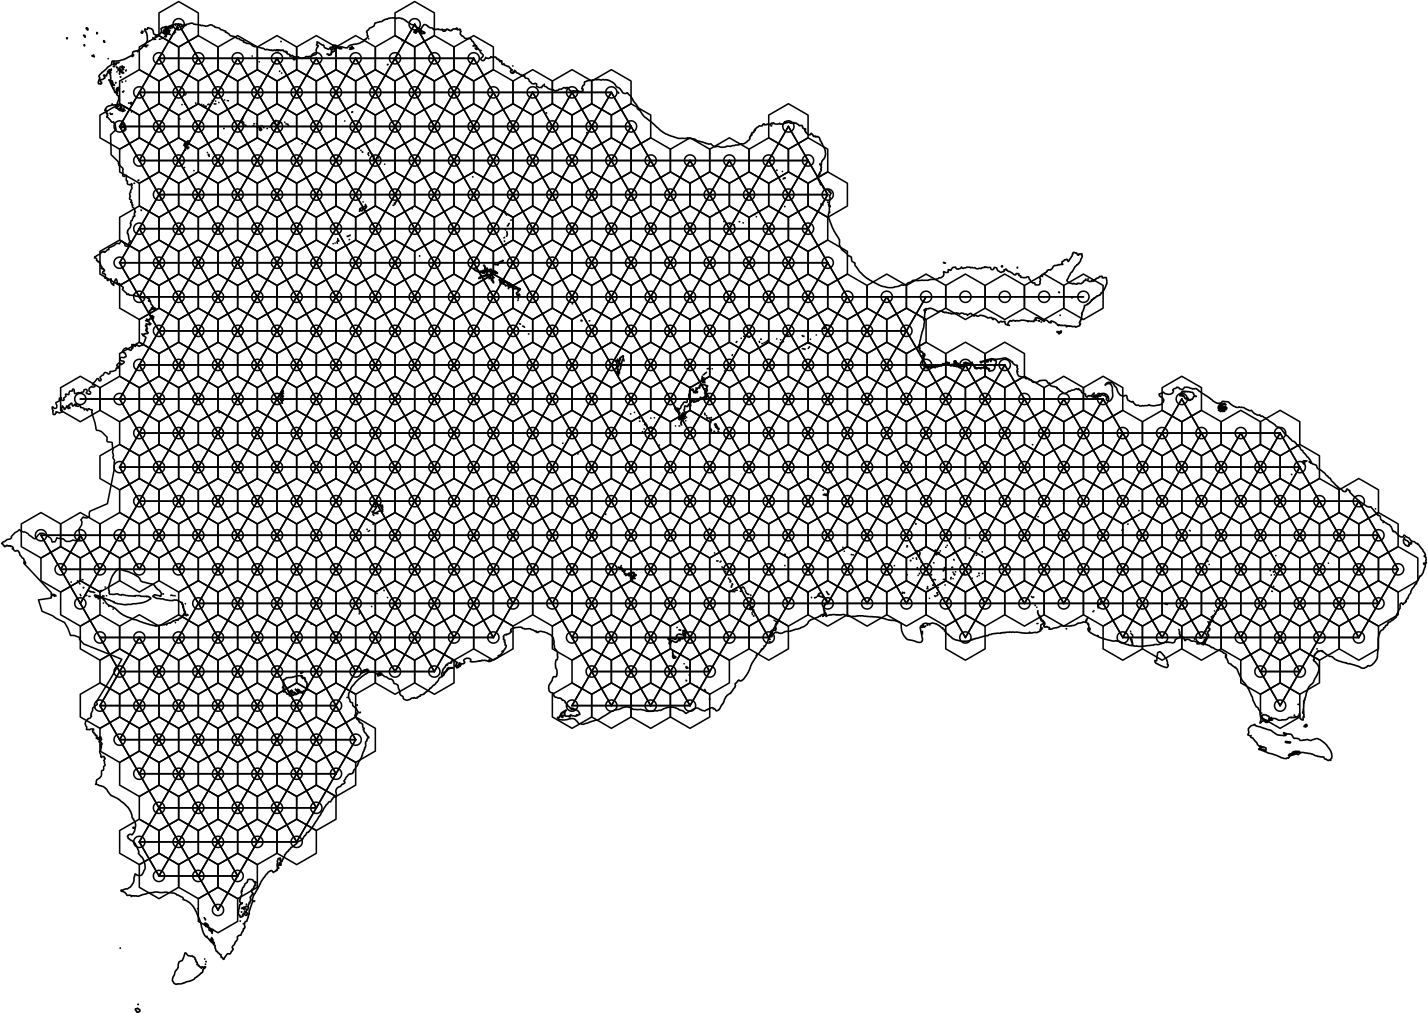
\includegraphics{img/modelling/lta-esda-1} \end{center}

\begin{Shaded}
\begin{Highlighting}[]
\FunctionTok{attr}\NormalTok{(grdnb, }\StringTok{"region.id"}\NormalTok{) }\OtherTok{\textless{}{-}}\NormalTok{ grdzonal}\SpecialCharTok{$}\NormalTok{ENLACE}
\NormalTok{grdww }\OtherTok{\textless{}{-}} \FunctionTok{nb2listw}\NormalTok{(grdnb, }\AttributeTok{zero.policy =}\NormalTok{ T)}
\NormalTok{grdww}
\DocumentationTok{\#\# Characteristics of weights list object:}
\DocumentationTok{\#\# Neighbour list object:}
\DocumentationTok{\#\# Number of regions: 482 }
\DocumentationTok{\#\# Number of nonzero links: 2622 }
\DocumentationTok{\#\# Percentage nonzero weights: 1.128596 }
\DocumentationTok{\#\# Average number of links: 5.439834 }
\DocumentationTok{\#\# }
\DocumentationTok{\#\# Weights style: W }
\DocumentationTok{\#\# Weights constants summary:}
\DocumentationTok{\#\#     n     nn  S0       S1       S2}
\DocumentationTok{\#\# W 482 232324 482 186.8356 1940.897}

\CommentTok{\# * Moran test per unit area (PUA)}
\NormalTok{grdzonal}\SpecialCharTok{$}\NormalTok{LOSS0118\_PUA\_PYR\_NORM }\OtherTok{\textless{}{-}} \FunctionTok{transformTukey}\NormalTok{(grdzonal}\SpecialCharTok{$}\NormalTok{LOSS0118\_PUA\_PYR }\SpecialCharTok{\%\textgreater{}\%}
    \FunctionTok{replace}\NormalTok{(}\FunctionTok{is.na}\NormalTok{(.), }\DecValTok{0}\NormalTok{), }\AttributeTok{plotit =}\NormalTok{ F)}
\DocumentationTok{\#\# }
\DocumentationTok{\#\#     lambda      W Shapiro.p.value}
\DocumentationTok{\#\# 414  0.325 0.9979          0.8116}
\DocumentationTok{\#\# }
\DocumentationTok{\#\# if (lambda \textgreater{}  0)\{TRANS = x \^{} lambda\} }
\DocumentationTok{\#\# if (lambda == 0)\{TRANS = log(x)\} }
\DocumentationTok{\#\# if (lambda \textless{}  0)\{TRANS = {-}1 * x \^{} lambda\}}
\CommentTok{\# lambda W Shapiro.p.value 414 0.325 0.9979 0.8116 if (lambda \textgreater{} 0)\{TRANS = x \^{}}
\CommentTok{\# lambda\} if (lambda == 0)\{TRANS = log(x)\} if (lambda \textless{} 0)\{TRANS = {-}1 * x \^{}}
\CommentTok{\# lambda\}}
\FunctionTok{moran.test}\NormalTok{(grdzonal}\SpecialCharTok{$}\NormalTok{LOSS0118\_PUA\_PYR\_NORM, }\AttributeTok{listw =}\NormalTok{ grdww, }\AttributeTok{na.action =}\NormalTok{ na.exclude,}
    \AttributeTok{zero.policy =}\NormalTok{ T)}
\DocumentationTok{\#\# }
\DocumentationTok{\#\#  Moran I test under randomisation}
\DocumentationTok{\#\# }
\DocumentationTok{\#\# data:  grdzonal$LOSS0118\_PUA\_PYR\_NORM  }
\DocumentationTok{\#\# weights: grdww    }
\DocumentationTok{\#\# }
\DocumentationTok{\#\# Moran I statistic standard deviate = 17.048, p{-}value \textless{} 2.2e{-}16}
\DocumentationTok{\#\# alternative hypothesis: greater}
\DocumentationTok{\#\# sample estimates:}
\DocumentationTok{\#\# Moran I statistic       Expectation          Variance }
\DocumentationTok{\#\#      0.4787566369     {-}0.0020790021      0.0007955173}

\CommentTok{\# * Moran test per unit area (PUA)}
\NormalTok{grdzonal}\SpecialCharTok{$}\NormalTok{LOSS1218\_PUA\_PYR\_NORM }\OtherTok{\textless{}{-}} \FunctionTok{transformTukey}\NormalTok{(grdzonal}\SpecialCharTok{$}\NormalTok{LOSS1218\_PUA\_PYR }\SpecialCharTok{\%\textgreater{}\%}
    \FunctionTok{replace}\NormalTok{(}\FunctionTok{is.na}\NormalTok{(.), }\DecValTok{0}\NormalTok{), }\AttributeTok{plotit =}\NormalTok{ F)}
\DocumentationTok{\#\# }
\DocumentationTok{\#\#     lambda      W Shapiro.p.value}
\DocumentationTok{\#\# 410  0.225 0.9977          0.7475}
\DocumentationTok{\#\# }
\DocumentationTok{\#\# if (lambda \textgreater{}  0)\{TRANS = x \^{} lambda\} }
\DocumentationTok{\#\# if (lambda == 0)\{TRANS = log(x)\} }
\DocumentationTok{\#\# if (lambda \textless{}  0)\{TRANS = {-}1 * x \^{} lambda\}}
\CommentTok{\# lambda W Shapiro.p.value 410 0.225 0.9977 0.7475 if (lambda \textgreater{} 0)\{TRANS = x \^{}}
\CommentTok{\# lambda\} if (lambda == 0)\{TRANS = log(x)\} if (lambda \textless{} 0)\{TRANS = {-}1 * x \^{}}
\CommentTok{\# lambda\}}
\FunctionTok{moran.test}\NormalTok{(grdzonal}\SpecialCharTok{$}\NormalTok{LOSS1218\_PUA\_PYR\_NORM, }\AttributeTok{listw =}\NormalTok{ grdww, }\AttributeTok{na.action =}\NormalTok{ na.exclude,}
    \AttributeTok{zero.policy =}\NormalTok{ T)}
\DocumentationTok{\#\# }
\DocumentationTok{\#\#  Moran I test under randomisation}
\DocumentationTok{\#\# }
\DocumentationTok{\#\# data:  grdzonal$LOSS1218\_PUA\_PYR\_NORM  }
\DocumentationTok{\#\# weights: grdww    }
\DocumentationTok{\#\# }
\DocumentationTok{\#\# Moran I statistic standard deviate = 17.045, p{-}value \textless{} 2.2e{-}16}
\DocumentationTok{\#\# alternative hypothesis: greater}
\DocumentationTok{\#\# sample estimates:}
\DocumentationTok{\#\# Moran I statistic       Expectation          Variance }
\DocumentationTok{\#\#      0.4785687944     {-}0.0020790021      0.0007951648}

\CommentTok{\# * Transformation of fires M6 per sq. km using Tukey\textquotesingle{}s Ladder of Powers}
\NormalTok{grdzonal}\SpecialCharTok{$}\NormalTok{NFIRESM6\_PSQKM\_PYR\_TLP }\OtherTok{\textless{}{-}} \FunctionTok{transformTukey}\NormalTok{(grdzonal}\SpecialCharTok{$}\NormalTok{NFIRESM6\_PSQKM\_PYR }\SpecialCharTok{\%\textgreater{}\%}
    \FunctionTok{replace}\NormalTok{(}\FunctionTok{is.na}\NormalTok{(.), }\DecValTok{0}\NormalTok{), }\AttributeTok{plotit =}\NormalTok{ F)}
\DocumentationTok{\#\# }
\DocumentationTok{\#\#     lambda      W Shapiro.p.value}
\DocumentationTok{\#\# 414  0.325 0.9833         2.5e{-}05}
\DocumentationTok{\#\# }
\DocumentationTok{\#\# if (lambda \textgreater{}  0)\{TRANS = x \^{} lambda\} }
\DocumentationTok{\#\# if (lambda == 0)\{TRANS = log(x)\} }
\DocumentationTok{\#\# if (lambda \textless{}  0)\{TRANS = {-}1 * x \^{} lambda\}}
\CommentTok{\# lambda W Shapiro.p.value 414 0.325 0.9833 2.5e{-}05 if (lambda \textgreater{} 0)\{TRANS = x \^{}}
\CommentTok{\# lambda\} if (lambda == 0)\{TRANS = log(x)\} if (lambda \textless{} 0)\{TRANS = {-}1 * x \^{}}
\CommentTok{\# lambda\}}

\CommentTok{\# * Transformation of fires V1 per sq. km using Tukey\textquotesingle{}s Ladder of Powers}
\NormalTok{grdzonal}\SpecialCharTok{$}\NormalTok{NFIRESV1\_PSQKM\_PYR\_TLP }\OtherTok{\textless{}{-}} \FunctionTok{transformTukey}\NormalTok{(grdzonal}\SpecialCharTok{$}\NormalTok{NFIRESV1\_PSQKM\_PYR }\SpecialCharTok{\%\textgreater{}\%}
    \FunctionTok{replace}\NormalTok{(}\FunctionTok{is.na}\NormalTok{(.), }\DecValTok{0}\NormalTok{), }\AttributeTok{plotit =}\NormalTok{ F)}
\DocumentationTok{\#\# }
\DocumentationTok{\#\#     lambda      W Shapiro.p.value}
\DocumentationTok{\#\# 413    0.3 0.9886        0.000823}
\DocumentationTok{\#\# }
\DocumentationTok{\#\# if (lambda \textgreater{}  0)\{TRANS = x \^{} lambda\} }
\DocumentationTok{\#\# if (lambda == 0)\{TRANS = log(x)\} }
\DocumentationTok{\#\# if (lambda \textless{}  0)\{TRANS = {-}1 * x \^{} lambda\}}
\CommentTok{\# lambda W Shapiro.p.value 413 0.3 0.9886 0.000823 if (lambda \textgreater{} 0)\{TRANS = x \^{}}
\CommentTok{\# lambda\} if (lambda == 0)\{TRANS = log(x)\} if (lambda \textless{} 0)\{TRANS = {-}1 * x \^{}}
\CommentTok{\# lambda\}}
\FunctionTok{moran.test}\NormalTok{(grdzonal}\SpecialCharTok{$}\NormalTok{NFIRESM6\_PSQKM\_PYR\_TLP, }\AttributeTok{listw =}\NormalTok{ grdww, }\AttributeTok{na.action =}\NormalTok{ na.exclude,}
    \AttributeTok{zero.policy =}\NormalTok{ T)}
\DocumentationTok{\#\# }
\DocumentationTok{\#\#  Moran I test under randomisation}
\DocumentationTok{\#\# }
\DocumentationTok{\#\# data:  grdzonal$NFIRESM6\_PSQKM\_PYR\_TLP  }
\DocumentationTok{\#\# weights: grdww    }
\DocumentationTok{\#\# }
\DocumentationTok{\#\# Moran I statistic standard deviate = 18.585, p{-}value \textless{} 2.2e{-}16}
\DocumentationTok{\#\# alternative hypothesis: greater}
\DocumentationTok{\#\# sample estimates:}
\DocumentationTok{\#\# Moran I statistic       Expectation          Variance }
\DocumentationTok{\#\#      0.5219024882     {-}0.0020790021      0.0007949039}
\FunctionTok{moran.test}\NormalTok{(grdzonal}\SpecialCharTok{$}\NormalTok{NFIRESV1\_PSQKM\_PYR\_TLP, }\AttributeTok{listw =}\NormalTok{ grdww, }\AttributeTok{na.action =}\NormalTok{ na.exclude,}
    \AttributeTok{zero.policy =}\NormalTok{ T)}
\DocumentationTok{\#\# }
\DocumentationTok{\#\#  Moran I test under randomisation}
\DocumentationTok{\#\# }
\DocumentationTok{\#\# data:  grdzonal$NFIRESV1\_PSQKM\_PYR\_TLP  }
\DocumentationTok{\#\# weights: grdww    }
\DocumentationTok{\#\# }
\DocumentationTok{\#\# Moran I statistic standard deviate = 18.272, p{-}value \textless{} 2.2e{-}16}
\DocumentationTok{\#\# alternative hypothesis: greater}
\DocumentationTok{\#\# sample estimates:}
\DocumentationTok{\#\# Moran I statistic       Expectation          Variance }
\DocumentationTok{\#\#      0.5130675981     {-}0.0020790021      0.0007948482}

\CommentTok{\# * Moran plot}
\NormalTok{mploss0118 }\OtherTok{\textless{}{-}} \FunctionTok{moran.plot}\NormalTok{(}\AttributeTok{x =} \FunctionTok{replace\_na}\NormalTok{(grdzonal}\SpecialCharTok{$}\NormalTok{LOSS0118\_PUA\_PYR\_NORM, }\DecValTok{0}\NormalTok{), }\AttributeTok{listw =}\NormalTok{ grdww,}
    \AttributeTok{zero.policy =}\NormalTok{ T, }\AttributeTok{quiet =}\NormalTok{ T, }\AttributeTok{xlab =} \StringTok{"Average forest loss per unit{-}area per year}\SpecialCharTok{\textbackslash{}n}\StringTok{of the period 2001{-}2018 (transformed)"}\NormalTok{,}
    \AttributeTok{ylab =} \StringTok{"Spatially lagged variable"}\NormalTok{, }\AttributeTok{return\_df =}\NormalTok{ T)}
\end{Highlighting}
\end{Shaded}

\begin{center}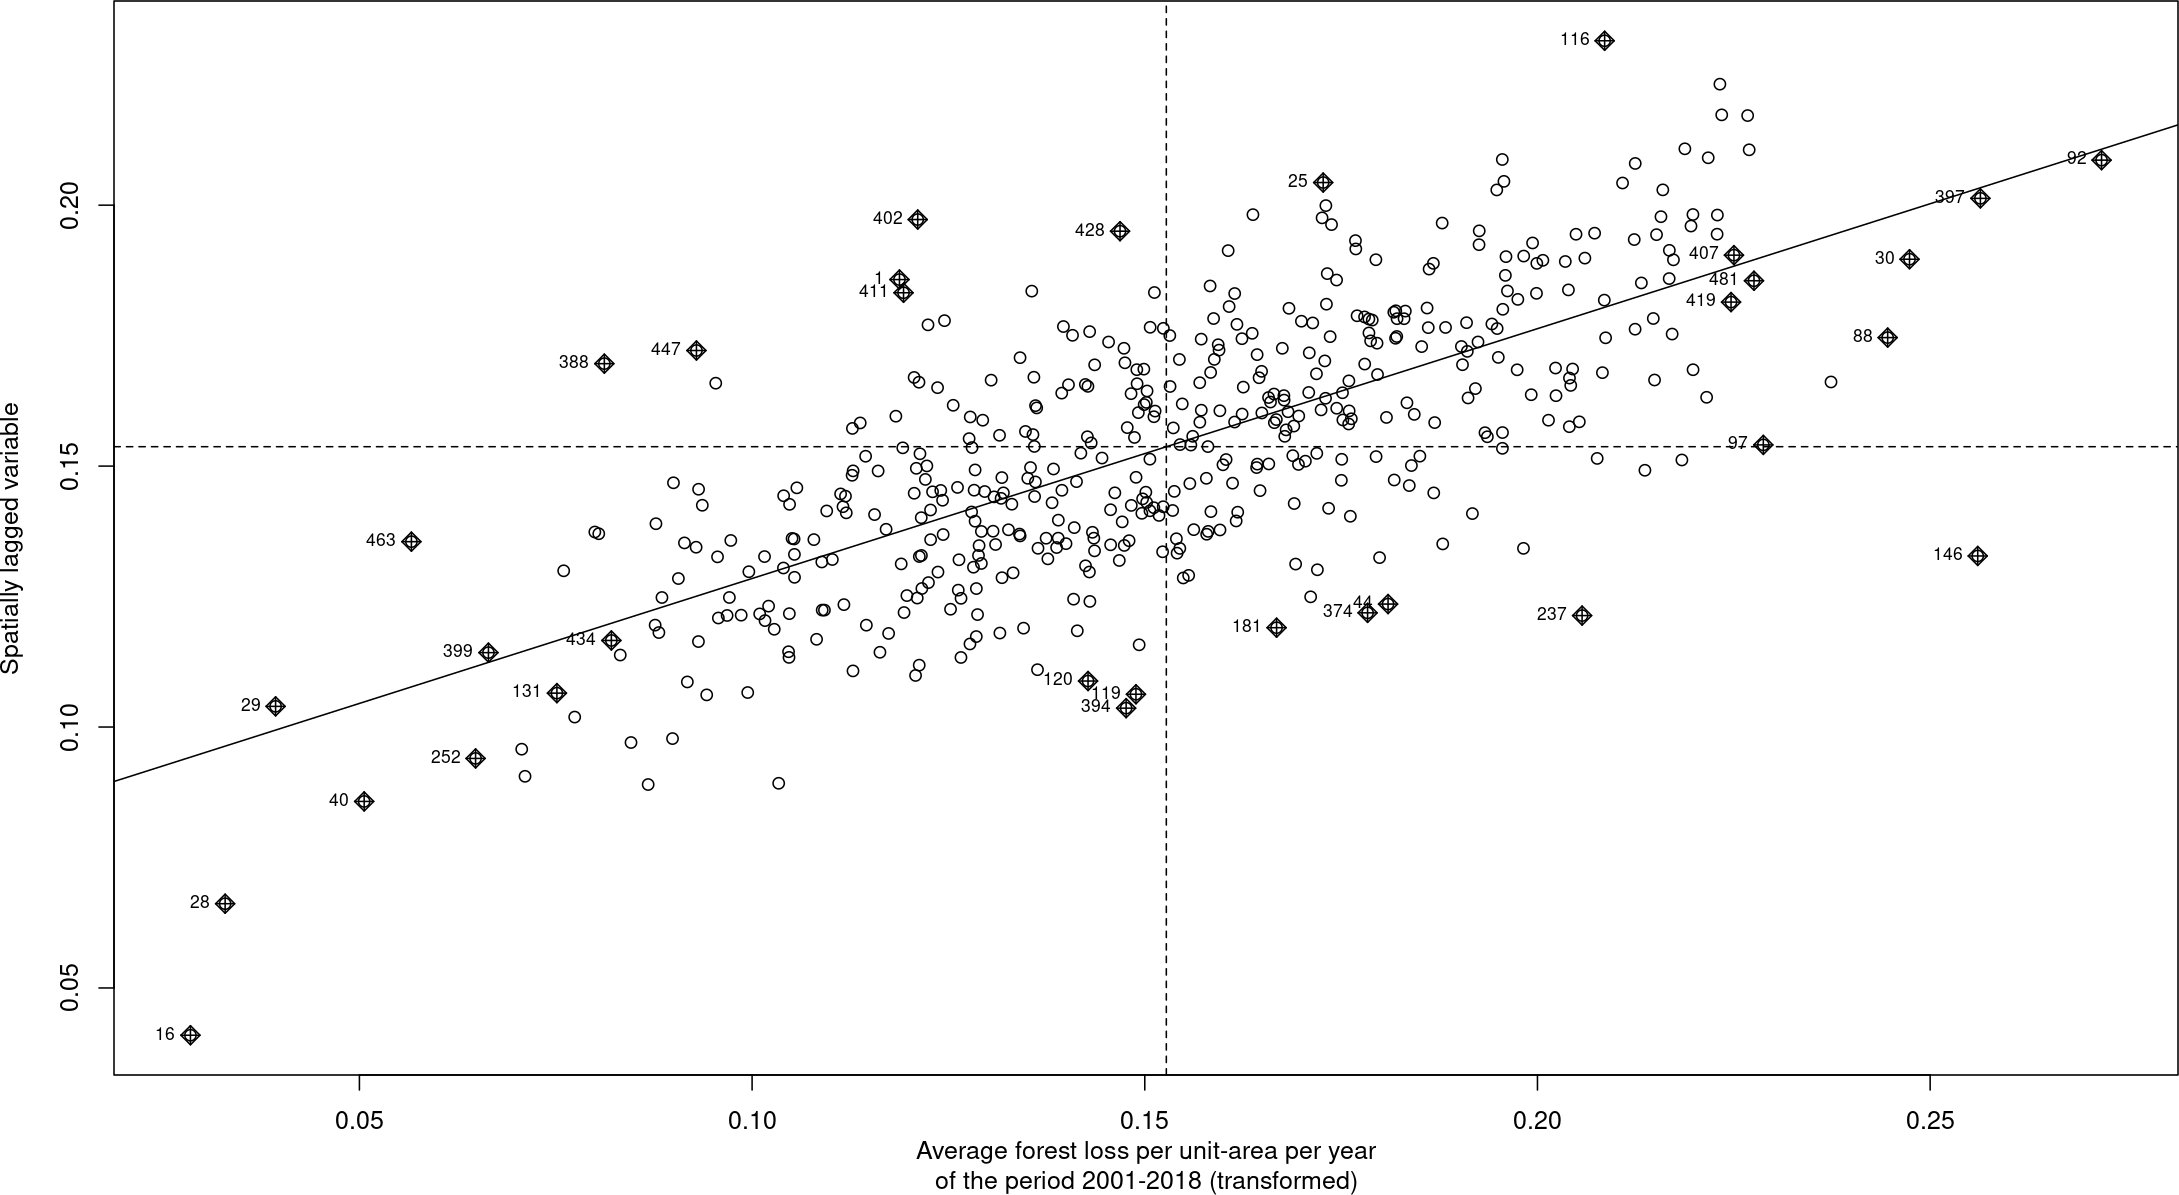
\includegraphics{img/modelling/lta-esda-2} \end{center}

\begin{Shaded}
\begin{Highlighting}[]
\NormalTok{mpfiresm60118 }\OtherTok{\textless{}{-}} \FunctionTok{moran.plot}\NormalTok{(}\AttributeTok{x =} \FunctionTok{replace\_na}\NormalTok{(grdzonal}\SpecialCharTok{$}\NormalTok{NFIRESM6\_PSQKM\_PYR\_TLP, }\DecValTok{0}\NormalTok{), }\AttributeTok{listw =}\NormalTok{ grdww,}
    \AttributeTok{zero.policy =}\NormalTok{ T, }\AttributeTok{quiet =}\NormalTok{ T, }\AttributeTok{xlab =} \StringTok{"Average number of fires M6 per square km per year}\SpecialCharTok{\textbackslash{}n}\StringTok{of the period 2001{-}2018 (transformed)"}\NormalTok{,}
    \AttributeTok{ylab =} \StringTok{"Spatially lagged variable"}\NormalTok{, }\AttributeTok{return\_df =}\NormalTok{ T)}
\end{Highlighting}
\end{Shaded}

\begin{center}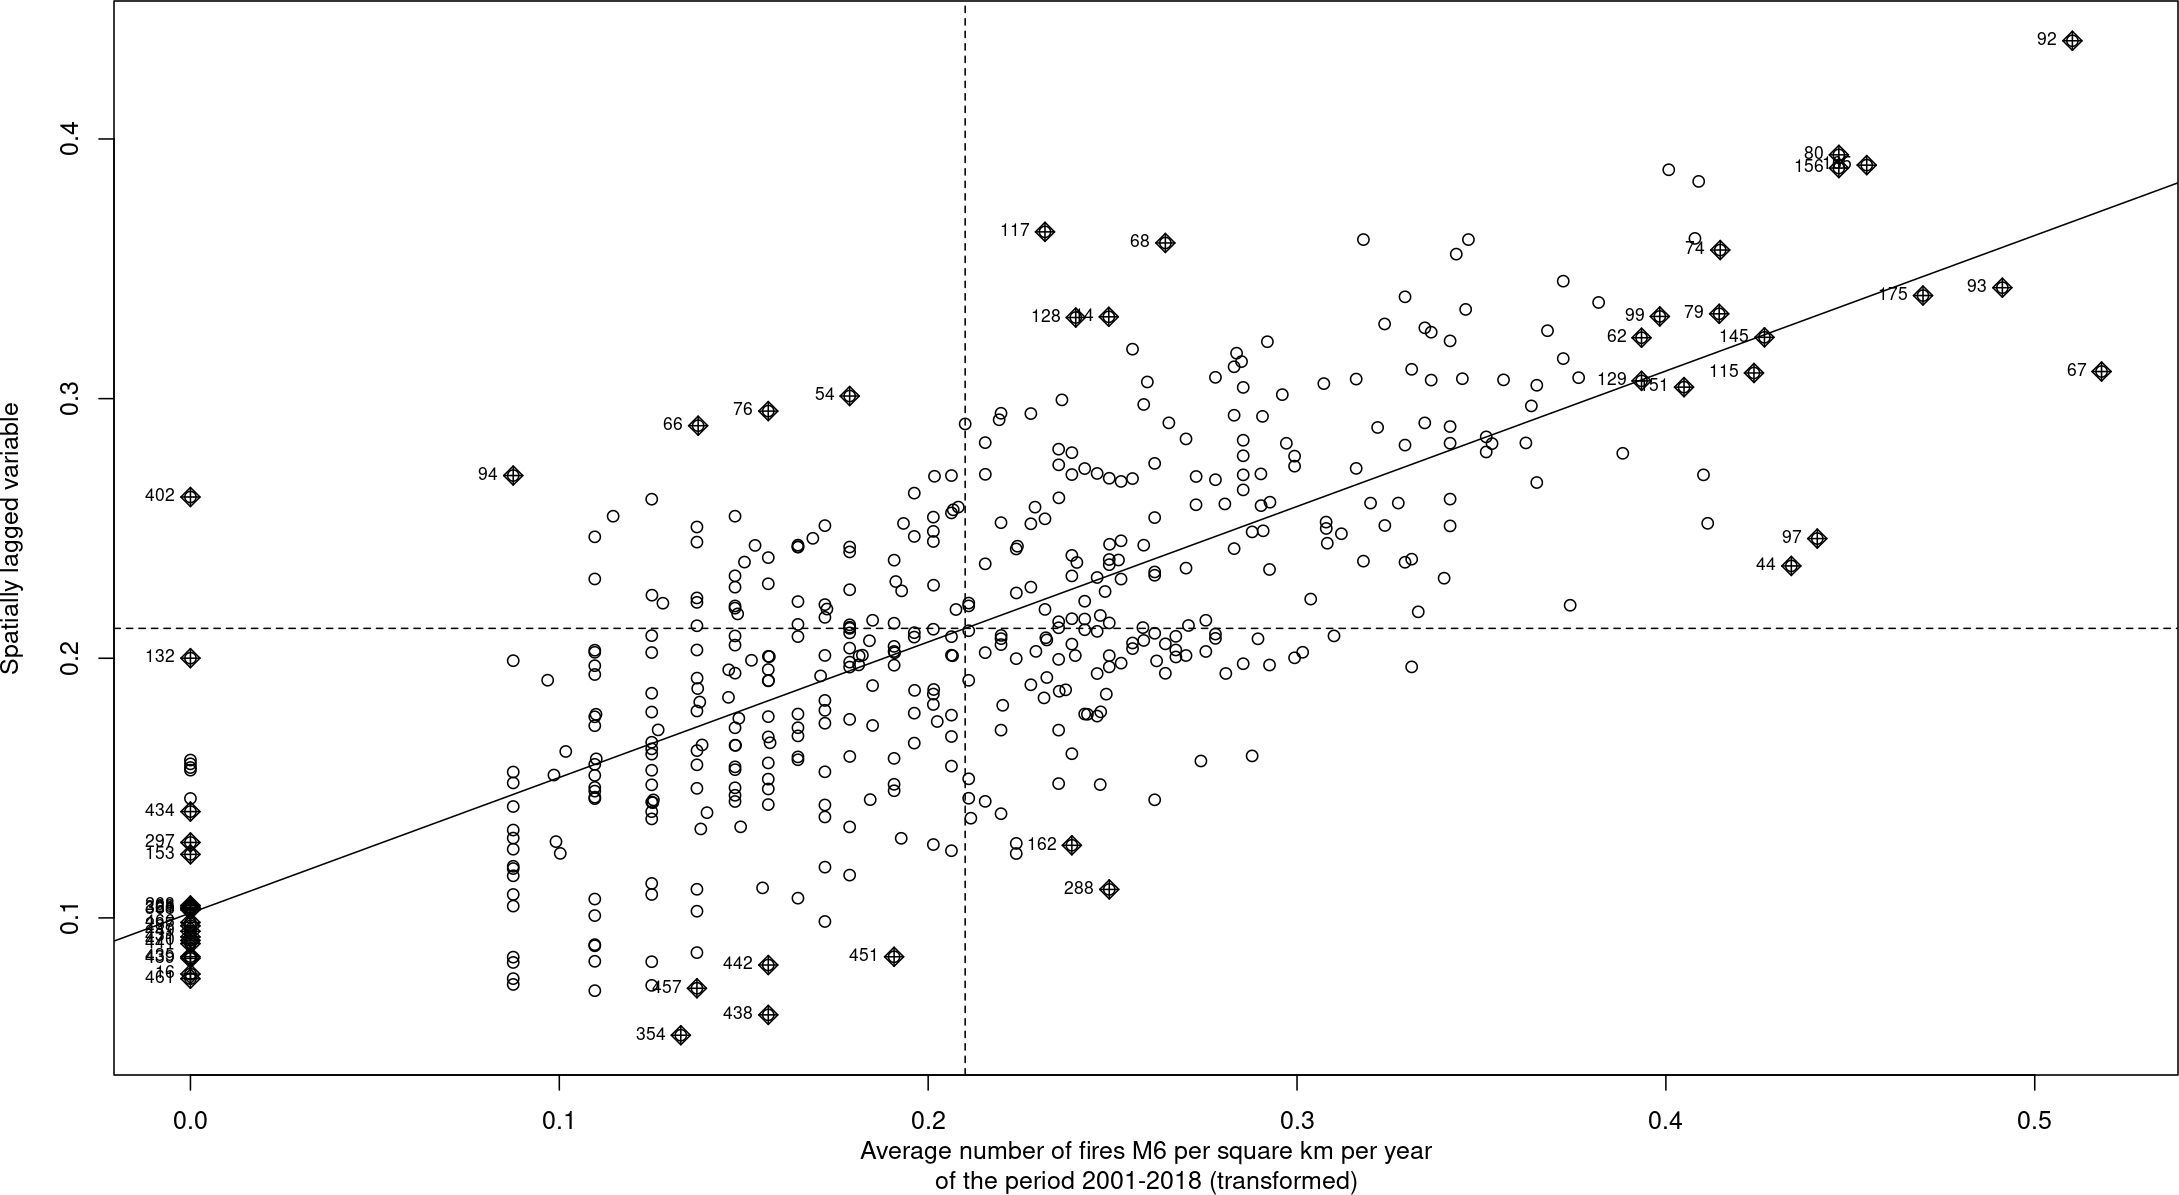
\includegraphics{img/modelling/lta-esda-3} \end{center}

\begin{Shaded}
\begin{Highlighting}[]
\NormalTok{mploss1218 }\OtherTok{\textless{}{-}} \FunctionTok{moran.plot}\NormalTok{(}\AttributeTok{x =} \FunctionTok{replace\_na}\NormalTok{(grdzonal}\SpecialCharTok{$}\NormalTok{LOSS1218\_PUA\_PYR\_NORM, }\DecValTok{0}\NormalTok{), }\AttributeTok{listw =}\NormalTok{ grdww,}
    \AttributeTok{zero.policy =}\NormalTok{ T, }\AttributeTok{quiet =}\NormalTok{ T, }\AttributeTok{xlab =} \StringTok{"Average forest loss per unit{-}area per year}\SpecialCharTok{\textbackslash{}n}\StringTok{of the period 2012{-}2018 (transformed)"}\NormalTok{,}
    \AttributeTok{ylab =} \StringTok{"Spatially lagged variable"}\NormalTok{, }\AttributeTok{return\_df =}\NormalTok{ T)}
\end{Highlighting}
\end{Shaded}

\begin{center}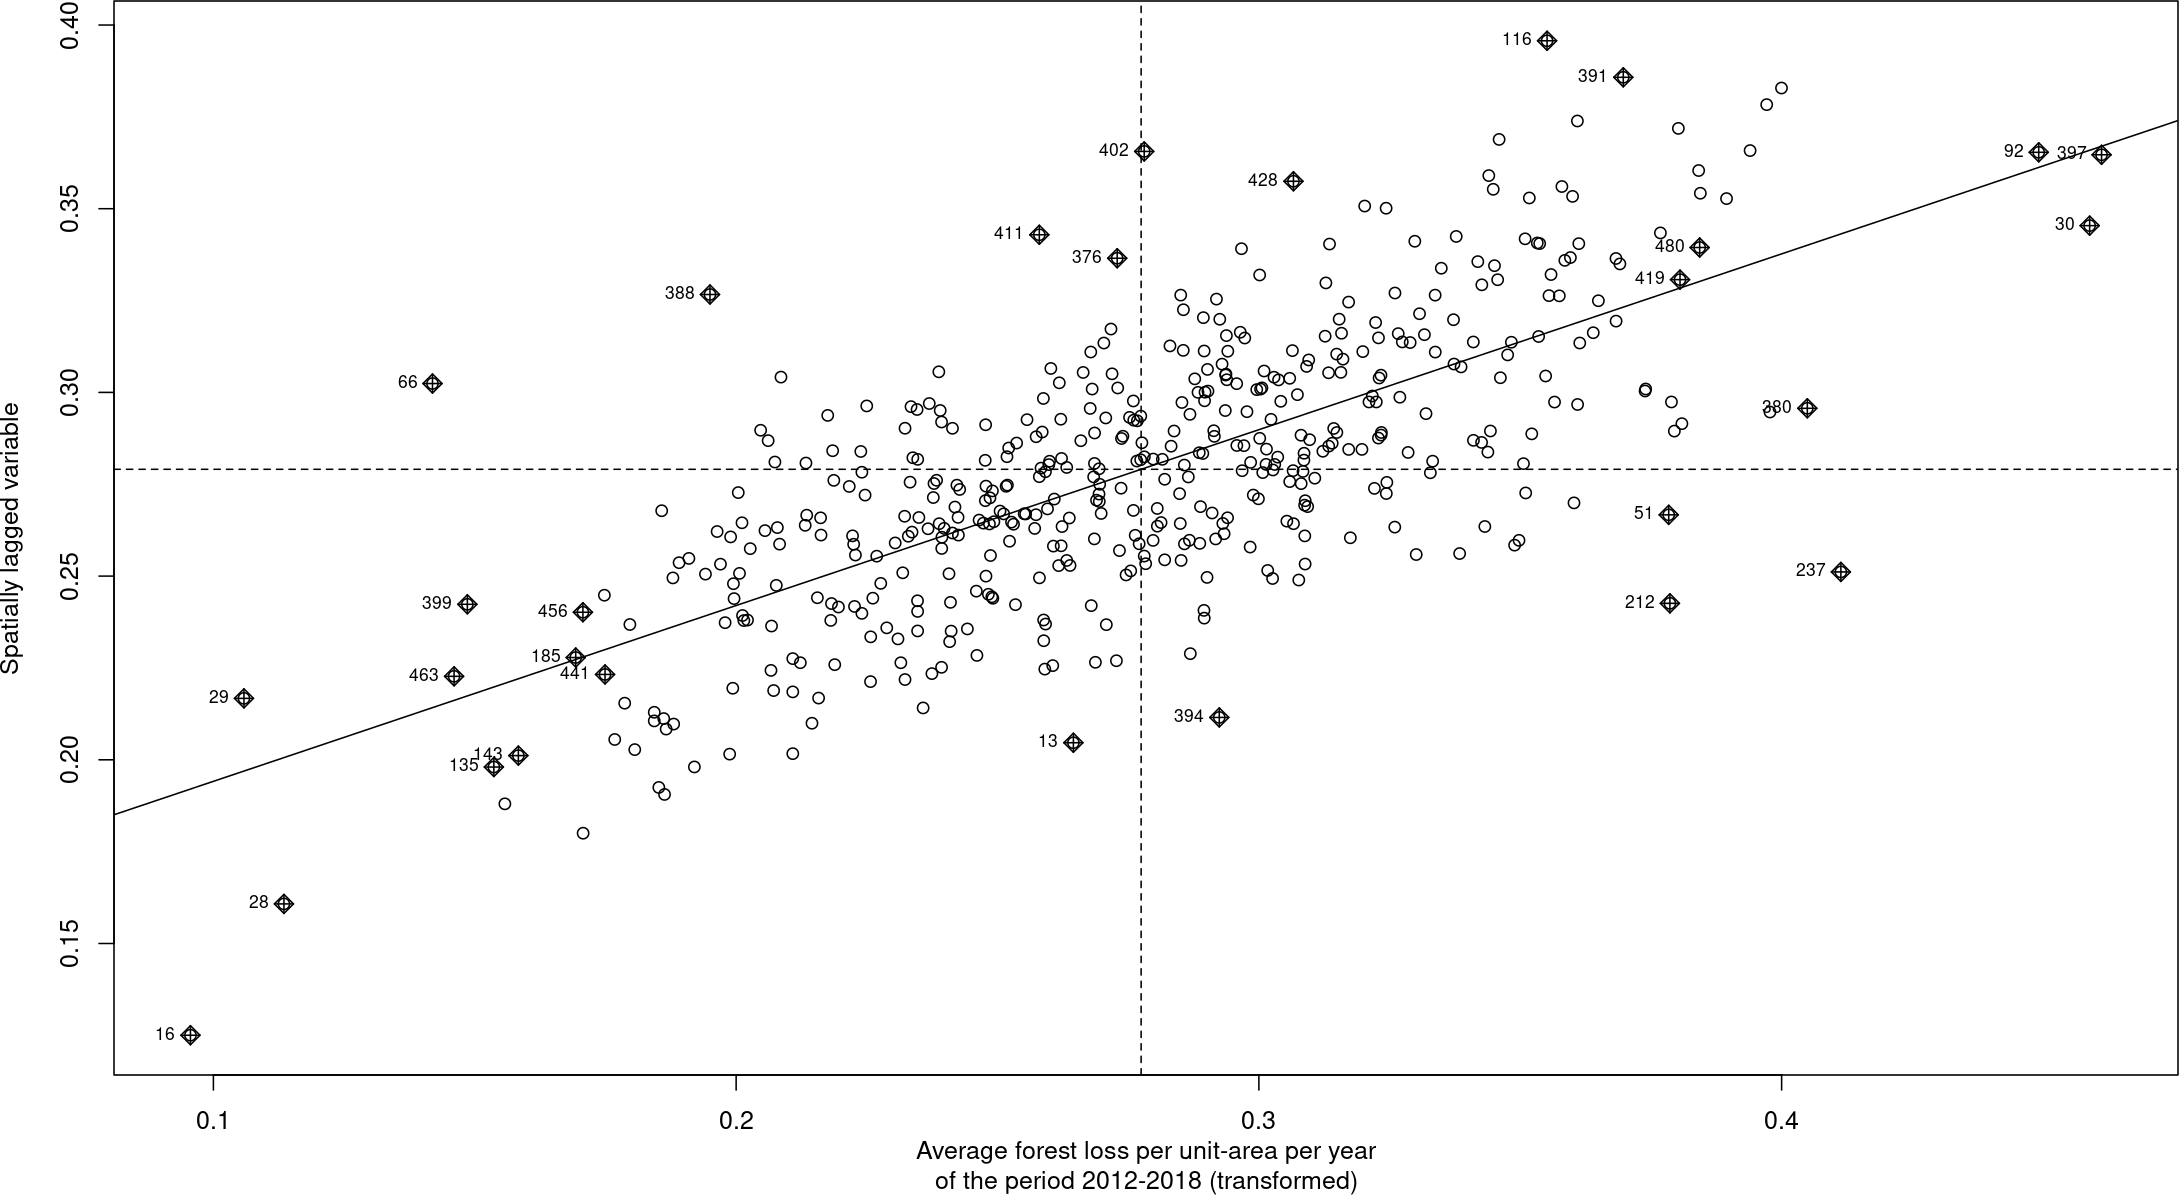
\includegraphics{img/modelling/lta-esda-4} \end{center}

\begin{Shaded}
\begin{Highlighting}[]
\NormalTok{mpfiresv11218 }\OtherTok{\textless{}{-}} \FunctionTok{moran.plot}\NormalTok{(}\AttributeTok{x =} \FunctionTok{replace\_na}\NormalTok{(grdzonal}\SpecialCharTok{$}\NormalTok{NFIRESV1\_PSQKM\_PYR\_TLP, }\DecValTok{0}\NormalTok{), }\AttributeTok{listw =}\NormalTok{ grdww,}
    \AttributeTok{zero.policy =}\NormalTok{ T, }\AttributeTok{quiet =}\NormalTok{ T, }\AttributeTok{xlab =} \StringTok{"Average number of fires V1 per square km per year}\SpecialCharTok{\textbackslash{}n}\StringTok{of the period 2012{-}2018 (transformed)"}\NormalTok{,}
    \AttributeTok{ylab =} \StringTok{"Spatially lagged variable"}\NormalTok{, }\AttributeTok{return\_df =}\NormalTok{ T)}
\end{Highlighting}
\end{Shaded}

\begin{center}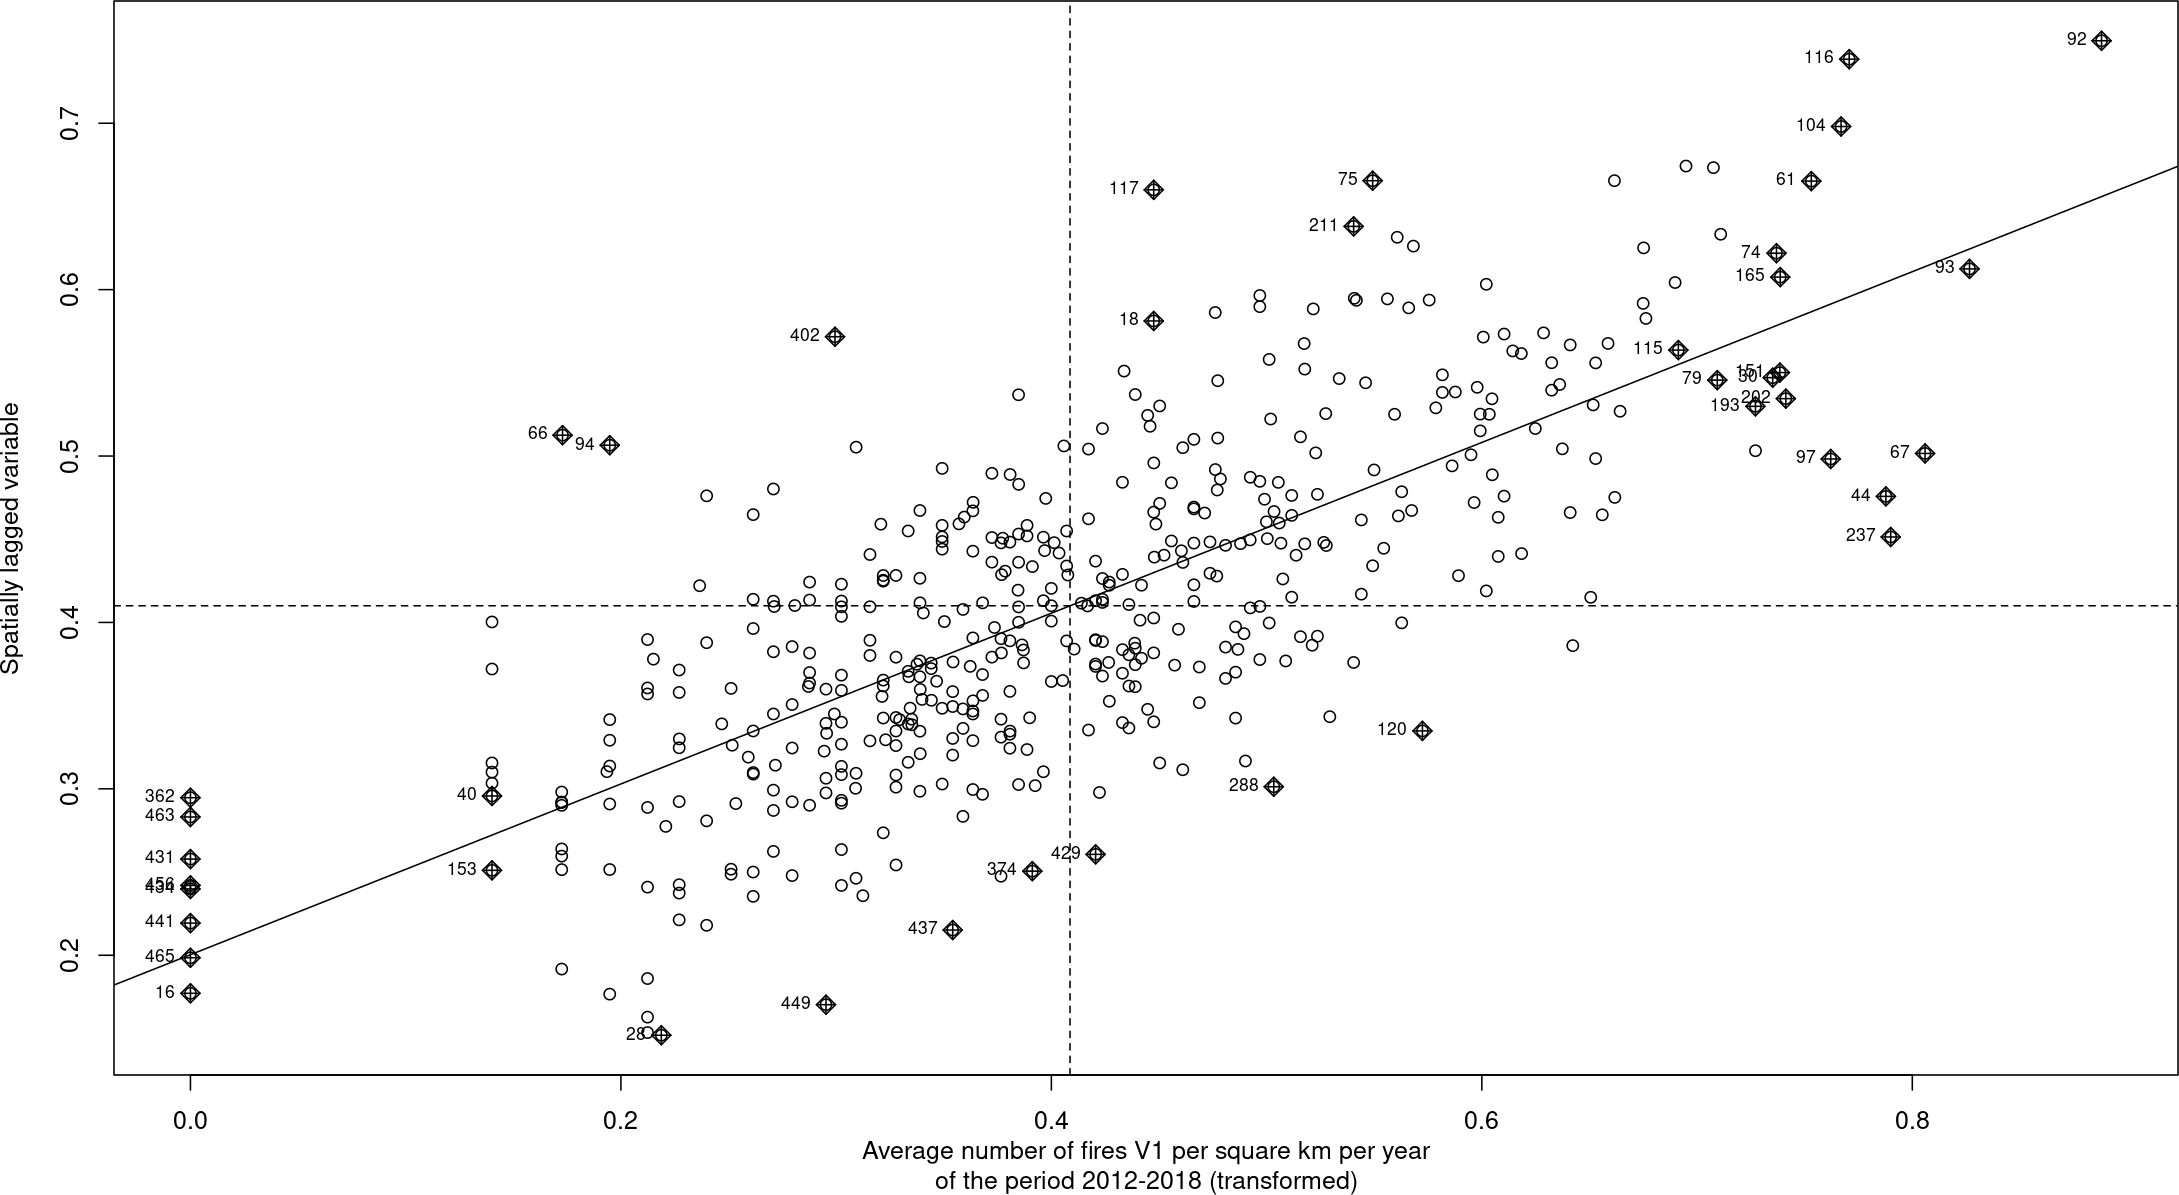
\includegraphics{img/modelling/lta-esda-5} \end{center}

\begin{Shaded}
\begin{Highlighting}[]

\CommentTok{\# gg Moran plot}
\NormalTok{\{}
\NormalTok{    all\_mp }\OtherTok{\textless{}{-}}\NormalTok{ plyr}\SpecialCharTok{::}\FunctionTok{ldply}\NormalTok{(}\FunctionTok{list}\NormalTok{(}\AttributeTok{mploss0118 =}\NormalTok{ mploss0118, }\AttributeTok{mploss1218 =}\NormalTok{ mploss1218,}
        \AttributeTok{mpfiresm60118 =}\NormalTok{ mpfiresm60118, }\AttributeTok{mpfiresv11218 =}\NormalTok{ mpfiresv11218), }\AttributeTok{.id =} \StringTok{"name"}\NormalTok{) }\SpecialCharTok{\%\textgreater{}\%}
        \FunctionTok{mutate}\NormalTok{(}\AttributeTok{name =} \FunctionTok{case\_when}\NormalTok{(name }\SpecialCharTok{==} \StringTok{"mploss0118"} \SpecialCharTok{\textasciitilde{}} \StringTok{"(A)"}\NormalTok{, name }\SpecialCharTok{==} \StringTok{"mploss1218"} \SpecialCharTok{\textasciitilde{}}
            \StringTok{"(B)"}\NormalTok{, name }\SpecialCharTok{==} \StringTok{"mpfiresm60118"} \SpecialCharTok{\textasciitilde{}} \StringTok{"(C)"}\NormalTok{, name }\SpecialCharTok{==} \StringTok{"mpfiresv11218"} \SpecialCharTok{\textasciitilde{}} \StringTok{"(D)"}\NormalTok{,}
            \ConstantTok{TRUE} \SpecialCharTok{\textasciitilde{}} \FunctionTok{as.character}\NormalTok{(x)))}
\NormalTok{    all\_mp\_sum }\OtherTok{\textless{}{-}}\NormalTok{ all\_mp }\SpecialCharTok{\%\textgreater{}\%}
        \FunctionTok{group\_by}\NormalTok{(name) }\SpecialCharTok{\%\textgreater{}\%}
        \FunctionTok{summarize}\NormalTok{(}\AttributeTok{x =} \FunctionTok{mean}\NormalTok{(x), }\AttributeTok{wx =} \FunctionTok{mean}\NormalTok{(wx))}
    \CommentTok{\# jpeg(\textquotesingle{}out/moran\_plots\_forest\_loss\_fires\_0118\_1218.jpg\textquotesingle{}, width = 3840,}
    \CommentTok{\# height = 2160, res = 300)}
    \FunctionTok{moran\_plot\_gg}\NormalTok{(}\AttributeTok{mp =}\NormalTok{ all\_mp, }\AttributeTok{mp\_sum =}\NormalTok{ all\_mp\_sum, }\AttributeTok{textsize =} \DecValTok{16}\NormalTok{)}
    \CommentTok{\# dev.off()}
\NormalTok{\}}
\end{Highlighting}
\end{Shaded}

\begin{center}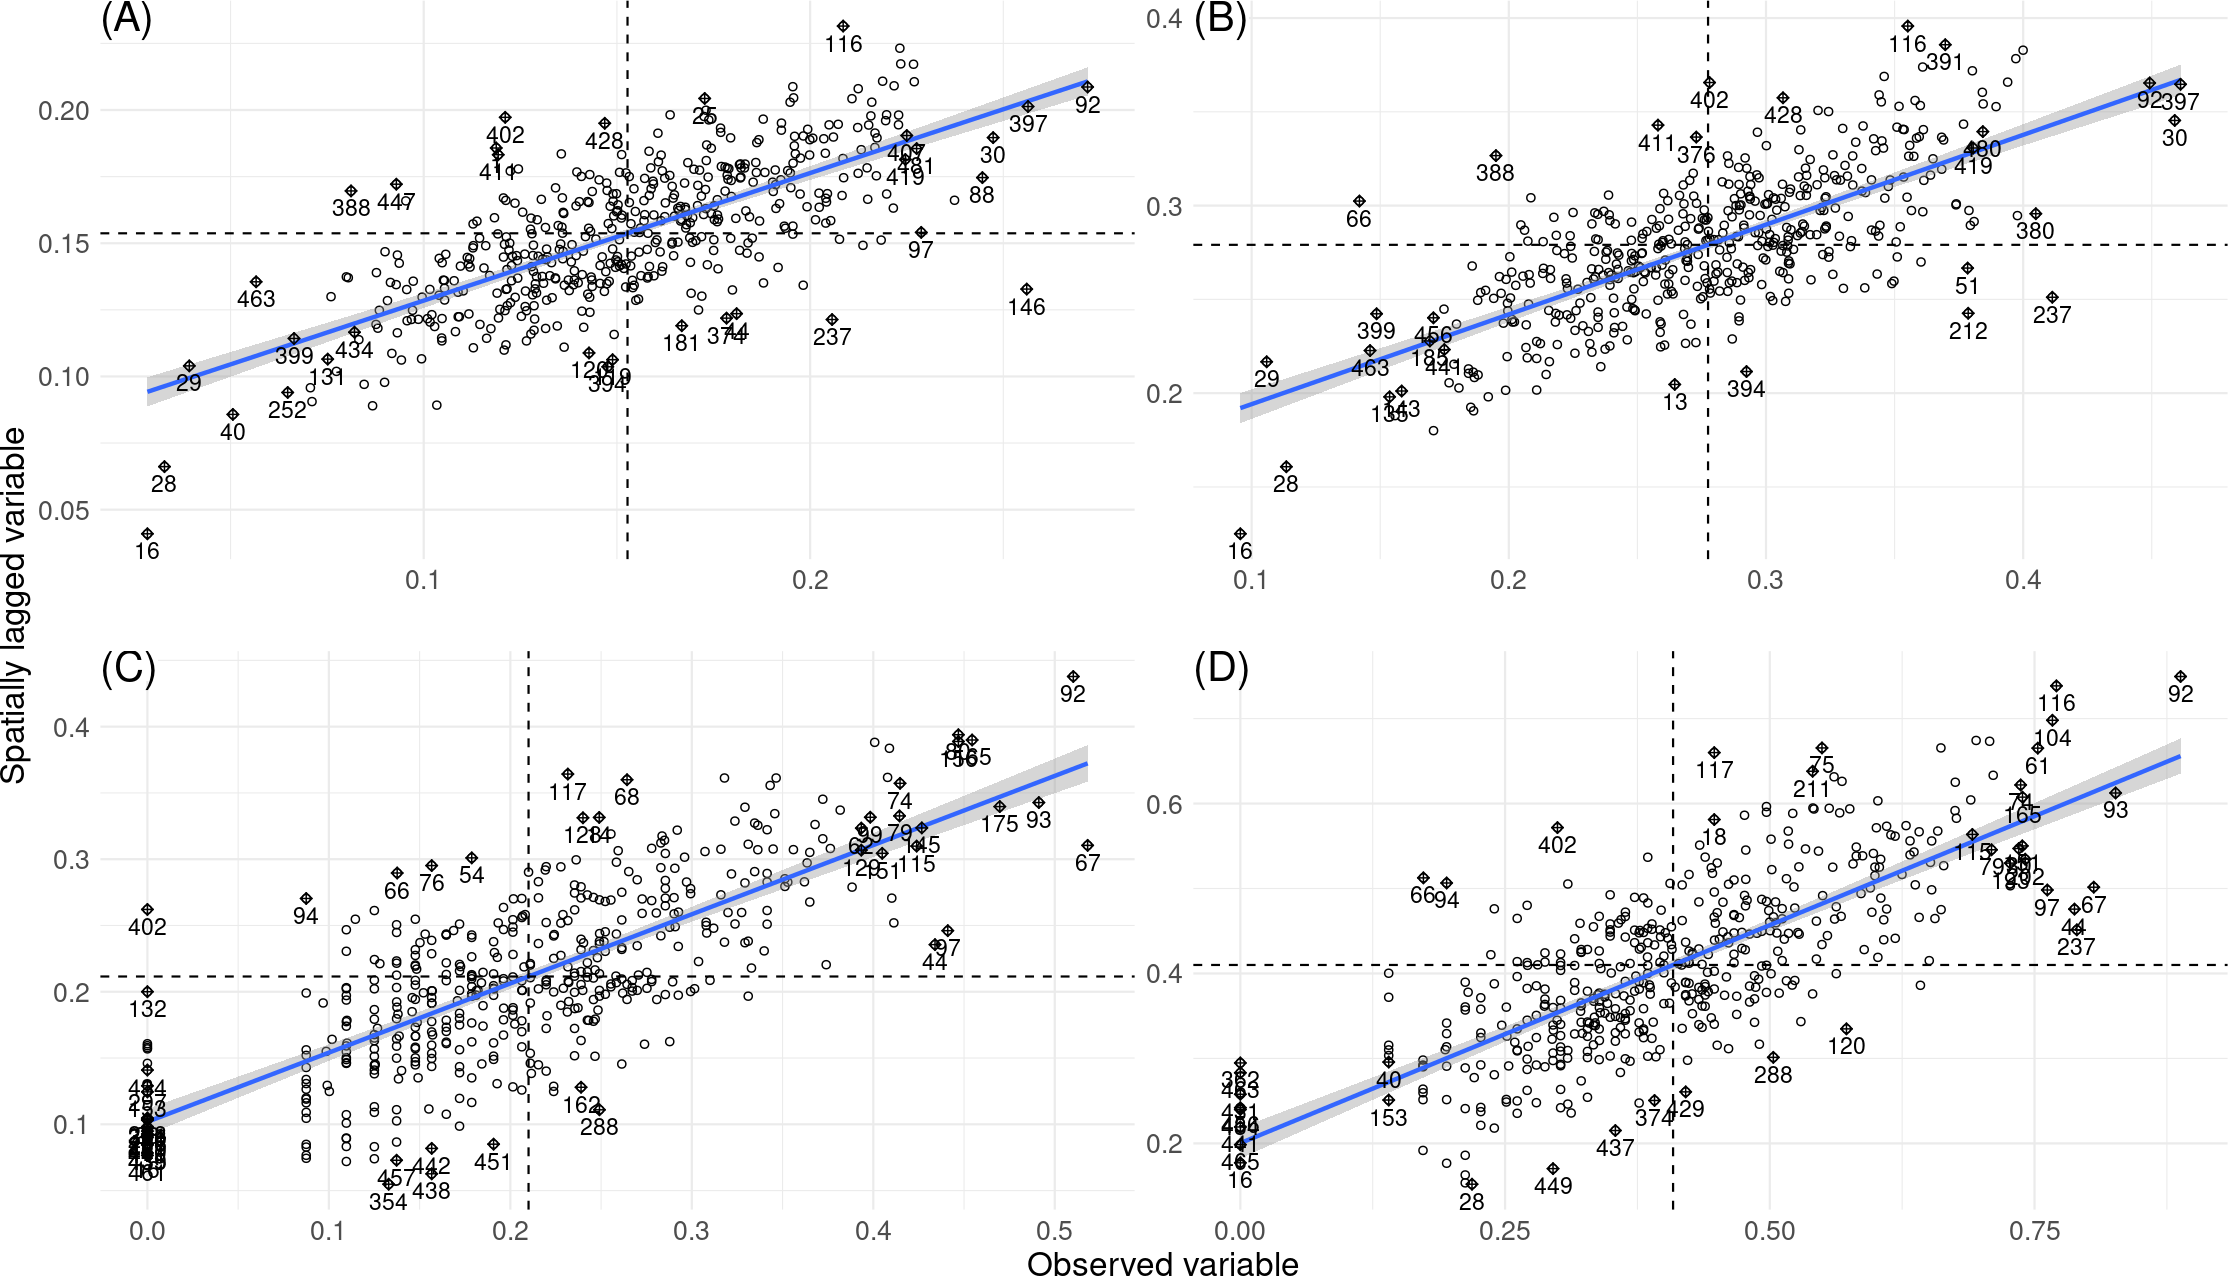
\includegraphics{img/modelling/lta-esda-6} \end{center}

\begin{Shaded}
\begin{Highlighting}[]

\CommentTok{\# * LISA Map LOSS0118\_PUA\_PYR\_NORM}
\NormalTok{grdlisamapl0118 }\OtherTok{\textless{}{-}} \FunctionTok{lisamap}\NormalTok{(}\AttributeTok{objesp =}\NormalTok{ grdzonal }\SpecialCharTok{\%\textgreater{}\%}
    \FunctionTok{replace}\NormalTok{(}\FunctionTok{is.na}\NormalTok{(.), }\DecValTok{0}\NormalTok{), }\AttributeTok{var =} \StringTok{"LOSS0118\_PUA\_PYR\_NORM"}\NormalTok{, }\AttributeTok{pesos =}\NormalTok{ grdww, }\AttributeTok{tituloleyenda =} \StringTok{"Significance}\SpecialCharTok{\textbackslash{}n}\StringTok{(}\SpecialCharTok{\textbackslash{}"}\StringTok{x{-}y}\SpecialCharTok{\textbackslash{}"}\StringTok{, read as}\SpecialCharTok{\textbackslash{}n}\StringTok{ }\SpecialCharTok{\textbackslash{}"}\StringTok{x}\SpecialCharTok{\textbackslash{}"}\StringTok{ surrounded}\SpecialCharTok{\textbackslash{}n}\StringTok{by }\SpecialCharTok{\textbackslash{}"}\StringTok{y}\SpecialCharTok{\textbackslash{}"}\StringTok{"}\NormalTok{,}
    \AttributeTok{leyenda =}\NormalTok{ T, }\AttributeTok{anchuratitulo =} \DecValTok{1000}\NormalTok{, }\AttributeTok{tamanotitulo =} \DecValTok{16}\NormalTok{, }\AttributeTok{fuentedatos =} \StringTok{"Hansen et al., 2013"}\NormalTok{,}
    \AttributeTok{titulomapa =} \FunctionTok{paste0}\NormalTok{(}\StringTok{"LISA clusters of forest loss per unit area per year, 2001{-}2018"}\NormalTok{))}
\CommentTok{\# grdlisamapl0118$grafico$layers \textless{}{-} c(grdlisamapl0118$grafico$layers,}
\CommentTok{\# geom\_sf(data=prov, fill = \textquotesingle{}transparent\textquotesingle{})[[1]])}
\NormalTok{grdlisamapl0118}\SpecialCharTok{$}\NormalTok{grafico}
\end{Highlighting}
\end{Shaded}

\begin{center}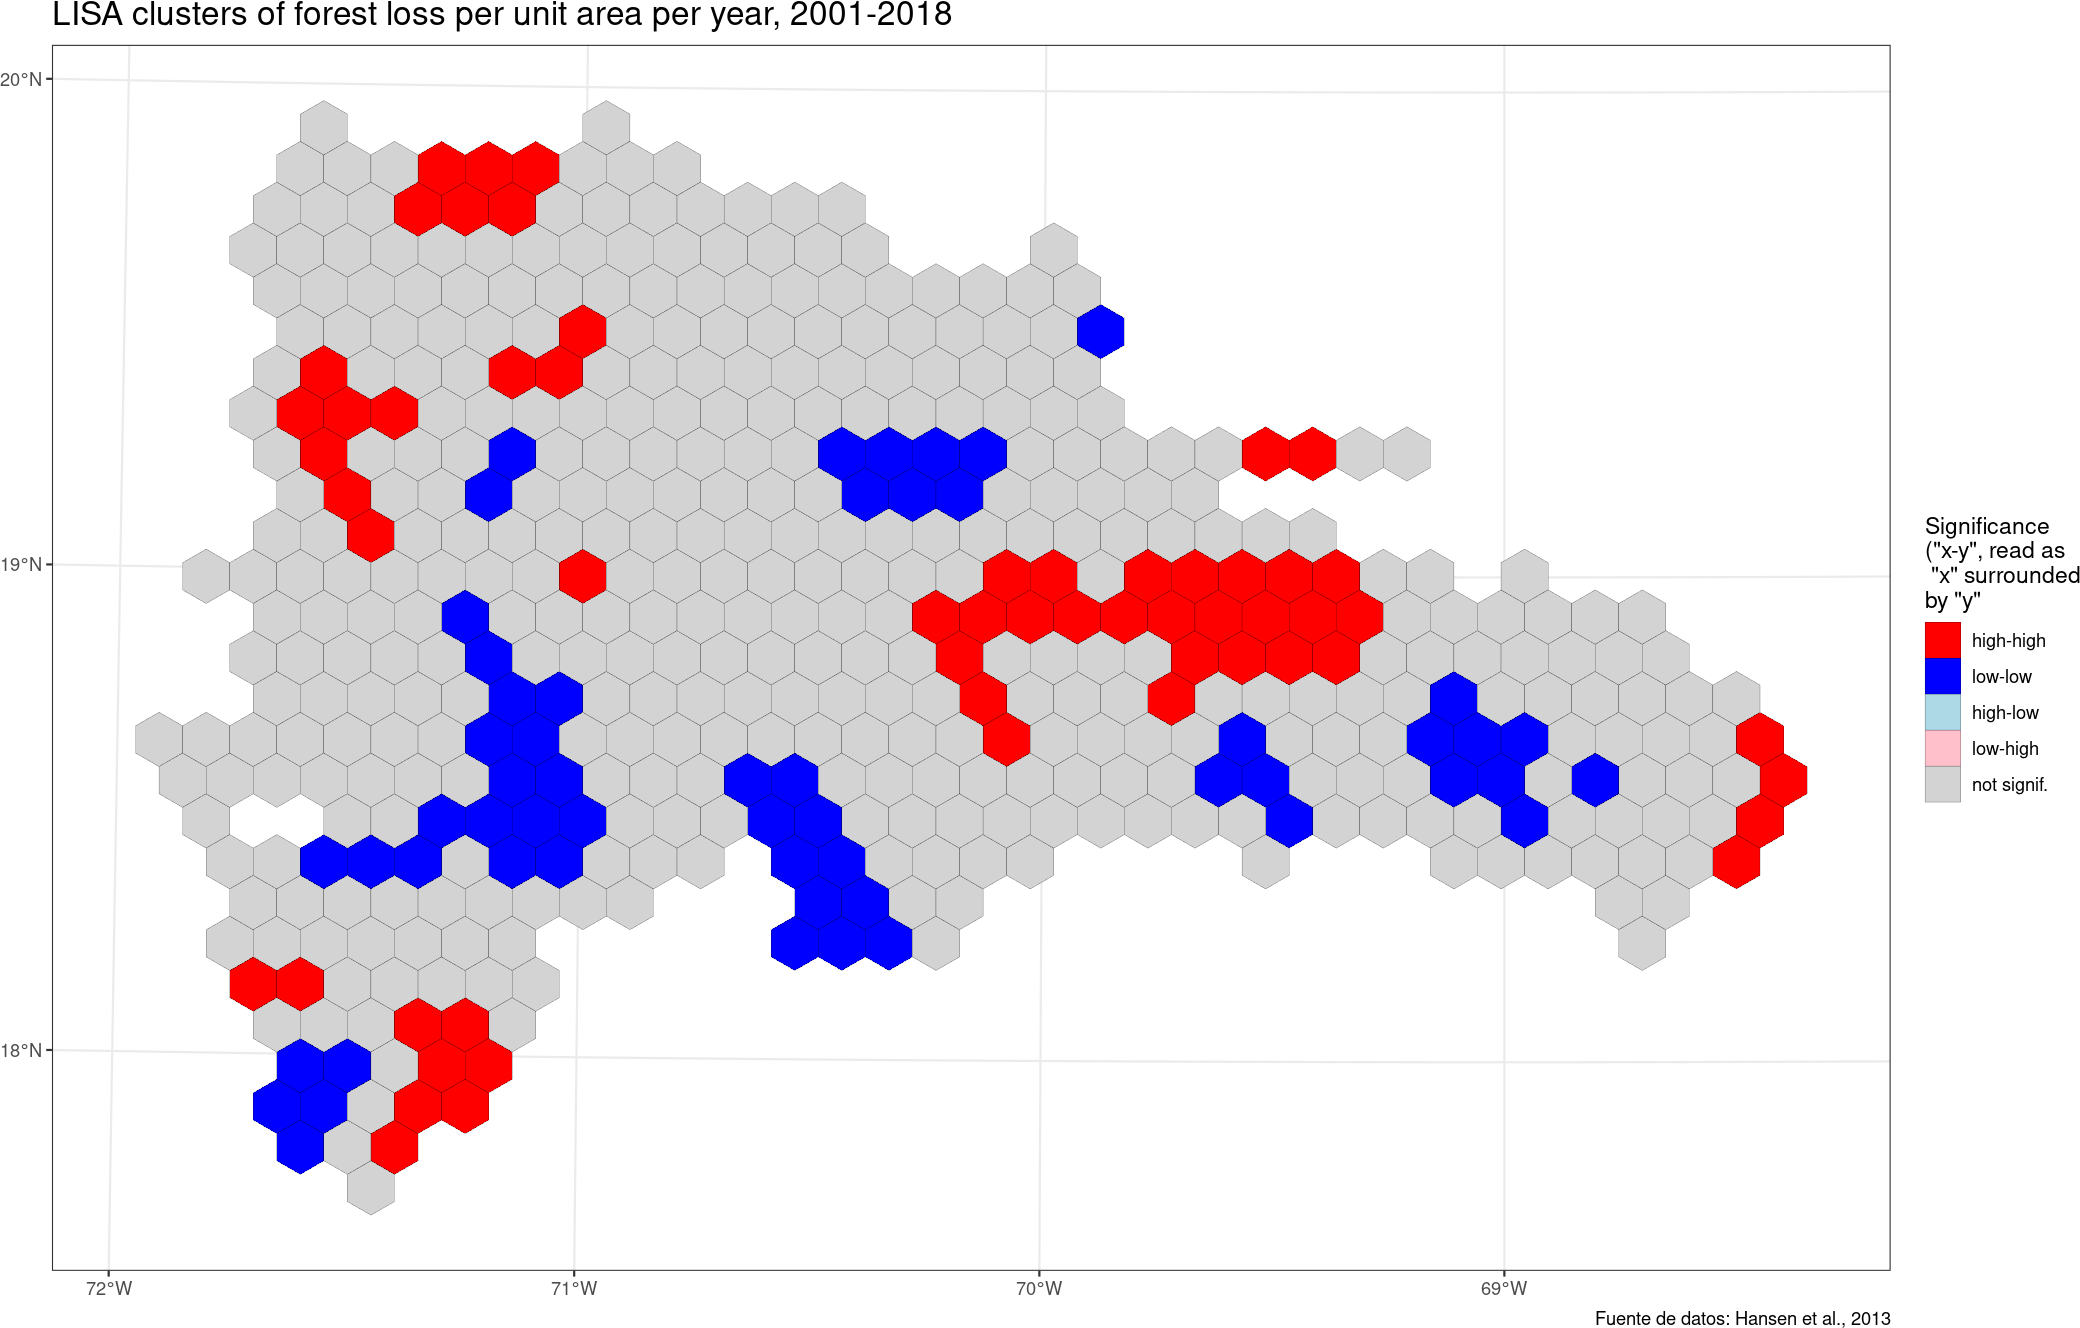
\includegraphics{img/modelling/lta-esda-7} \end{center}

\begin{Shaded}
\begin{Highlighting}[]

\CommentTok{\# * LISA Map FIRESM6\_PSQKM\_PYR per square km per year}
\NormalTok{grdlisamapfm6 }\OtherTok{\textless{}{-}} \FunctionTok{lisamap}\NormalTok{(}\AttributeTok{objesp =}\NormalTok{ grdzonal }\SpecialCharTok{\%\textgreater{}\%}
    \FunctionTok{replace}\NormalTok{(}\FunctionTok{is.na}\NormalTok{(.), }\DecValTok{0}\NormalTok{), }\AttributeTok{var =} \StringTok{"NFIRESM6\_PSQKM\_PYR"}\NormalTok{, }\AttributeTok{pesos =}\NormalTok{ grdww, }\AttributeTok{tituloleyenda =} \StringTok{"Significance}\SpecialCharTok{\textbackslash{}n}\StringTok{(}\SpecialCharTok{\textbackslash{}"}\StringTok{x{-}y}\SpecialCharTok{\textbackslash{}"}\StringTok{, read as}\SpecialCharTok{\textbackslash{}n}\StringTok{ }\SpecialCharTok{\textbackslash{}"}\StringTok{x}\SpecialCharTok{\textbackslash{}"}\StringTok{ surrounded}\SpecialCharTok{\textbackslash{}n}\StringTok{by }\SpecialCharTok{\textbackslash{}"}\StringTok{y}\SpecialCharTok{\textbackslash{}"}\StringTok{"}\NormalTok{,}
    \AttributeTok{leyenda =}\NormalTok{ T, }\AttributeTok{anchuratitulo =} \DecValTok{1000}\NormalTok{, }\AttributeTok{tamanotitulo =} \DecValTok{16}\NormalTok{, }\AttributeTok{fuentedatos =} \StringTok{"NASA, 2019"}\NormalTok{,}
    \AttributeTok{titulomapa =} \FunctionTok{paste0}\NormalTok{(}\StringTok{"LISA clusters of fires M6 per square km per year, 2001{-}2018"}\NormalTok{))}
\NormalTok{grdlisamapfm6}\SpecialCharTok{$}\NormalTok{grafico}\SpecialCharTok{$}\NormalTok{layers }\OtherTok{\textless{}{-}} \FunctionTok{c}\NormalTok{(grdlisamapfm6}\SpecialCharTok{$}\NormalTok{grafico}\SpecialCharTok{$}\NormalTok{layers, }\FunctionTok{geom\_sf}\NormalTok{(}\AttributeTok{data =}\NormalTok{ prov,}
    \AttributeTok{fill =} \StringTok{"transparent"}\NormalTok{)[[}\DecValTok{1}\NormalTok{]])}
\NormalTok{grdlisamapfm6}\SpecialCharTok{$}\NormalTok{grafico}
\end{Highlighting}
\end{Shaded}

\begin{center}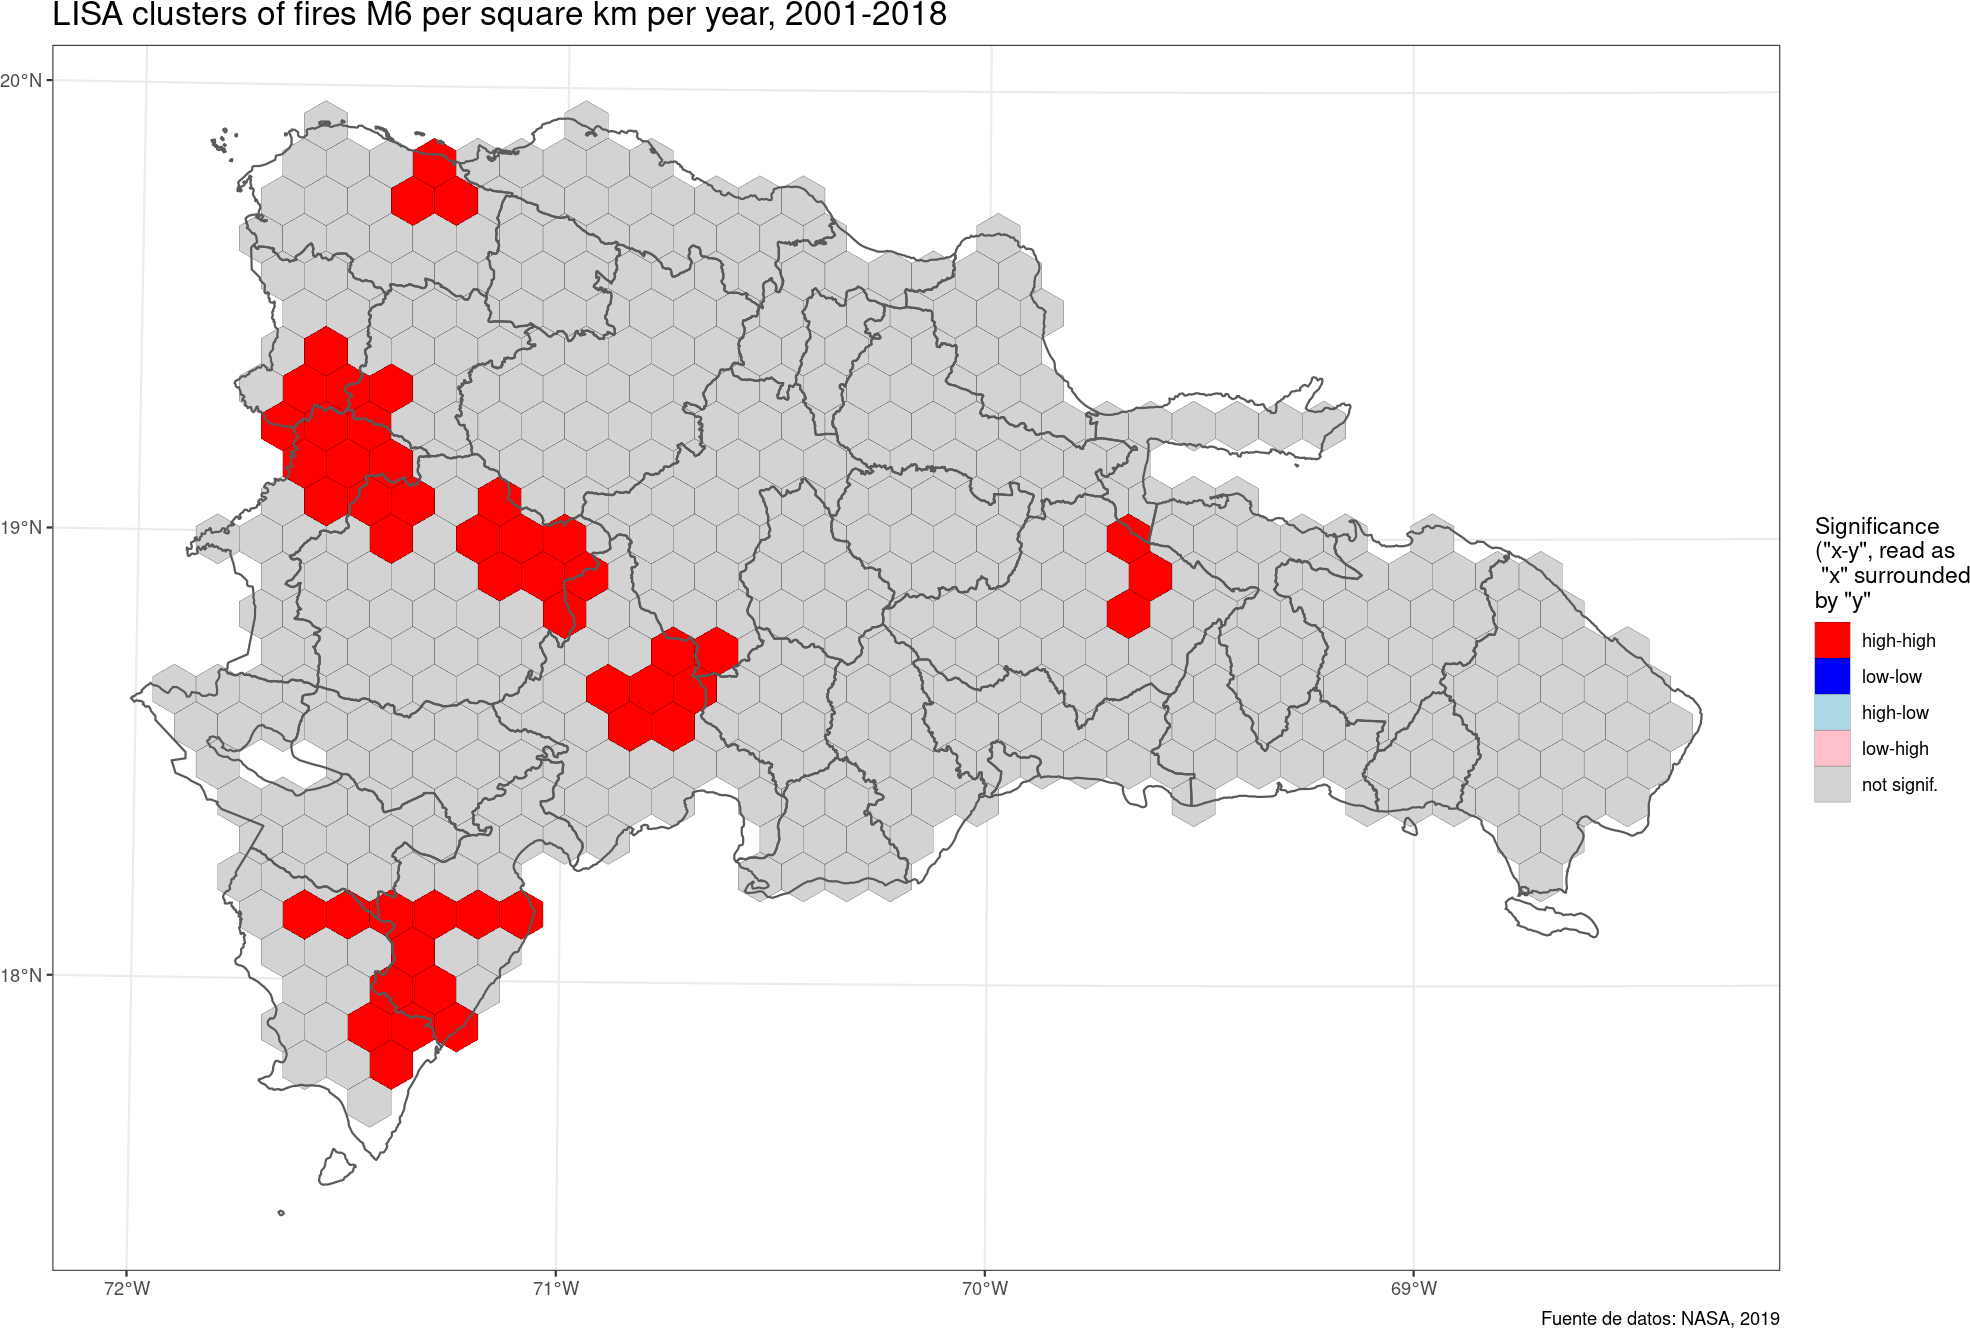
\includegraphics{img/modelling/lta-esda-8} \end{center}

\begin{Shaded}
\begin{Highlighting}[]

\CommentTok{\# * LISA Map FIRESM6\_PSQKM\_PYR\_TLP per square km per year}
\NormalTok{grdlisamapfm6tlp }\OtherTok{\textless{}{-}} \FunctionTok{lisamap}\NormalTok{(}\AttributeTok{objesp =}\NormalTok{ grdzonal }\SpecialCharTok{\%\textgreater{}\%}
    \FunctionTok{replace}\NormalTok{(}\FunctionTok{is.na}\NormalTok{(.), }\DecValTok{0}\NormalTok{), }\AttributeTok{var =} \StringTok{"NFIRESM6\_PSQKM\_PYR\_TLP"}\NormalTok{, }\AttributeTok{pesos =}\NormalTok{ grdww, }\AttributeTok{tituloleyenda =} \StringTok{"Significance}\SpecialCharTok{\textbackslash{}n}\StringTok{(}\SpecialCharTok{\textbackslash{}"}\StringTok{x{-}y}\SpecialCharTok{\textbackslash{}"}\StringTok{, read as}\SpecialCharTok{\textbackslash{}n}\StringTok{ }\SpecialCharTok{\textbackslash{}"}\StringTok{x}\SpecialCharTok{\textbackslash{}"}\StringTok{ surrounded}\SpecialCharTok{\textbackslash{}n}\StringTok{by }\SpecialCharTok{\textbackslash{}"}\StringTok{y}\SpecialCharTok{\textbackslash{}"}\StringTok{"}\NormalTok{,}
    \AttributeTok{leyenda =}\NormalTok{ T, }\AttributeTok{anchuratitulo =} \DecValTok{1000}\NormalTok{, }\AttributeTok{tamanotitulo =} \DecValTok{16}\NormalTok{, }\AttributeTok{fuentedatos =} \StringTok{"NASA, 2019"}\NormalTok{,}
    \AttributeTok{titulomapa =} \FunctionTok{paste0}\NormalTok{(}\StringTok{"LISA clusters of fires M6 (transformed) per square km per year, 2001{-}2018"}\NormalTok{))}
\NormalTok{grdlisamapfm6tlp}\SpecialCharTok{$}\NormalTok{grafico}\SpecialCharTok{$}\NormalTok{layers }\OtherTok{\textless{}{-}} \FunctionTok{c}\NormalTok{(grdlisamapfm6tlp}\SpecialCharTok{$}\NormalTok{grafico}\SpecialCharTok{$}\NormalTok{layers, }\FunctionTok{geom\_sf}\NormalTok{(}\AttributeTok{data =}\NormalTok{ prov,}
    \AttributeTok{fill =} \StringTok{"transparent"}\NormalTok{)[[}\DecValTok{1}\NormalTok{]])}
\NormalTok{grdlisamapfm6tlp}\SpecialCharTok{$}\NormalTok{grafico}
\end{Highlighting}
\end{Shaded}

\begin{center}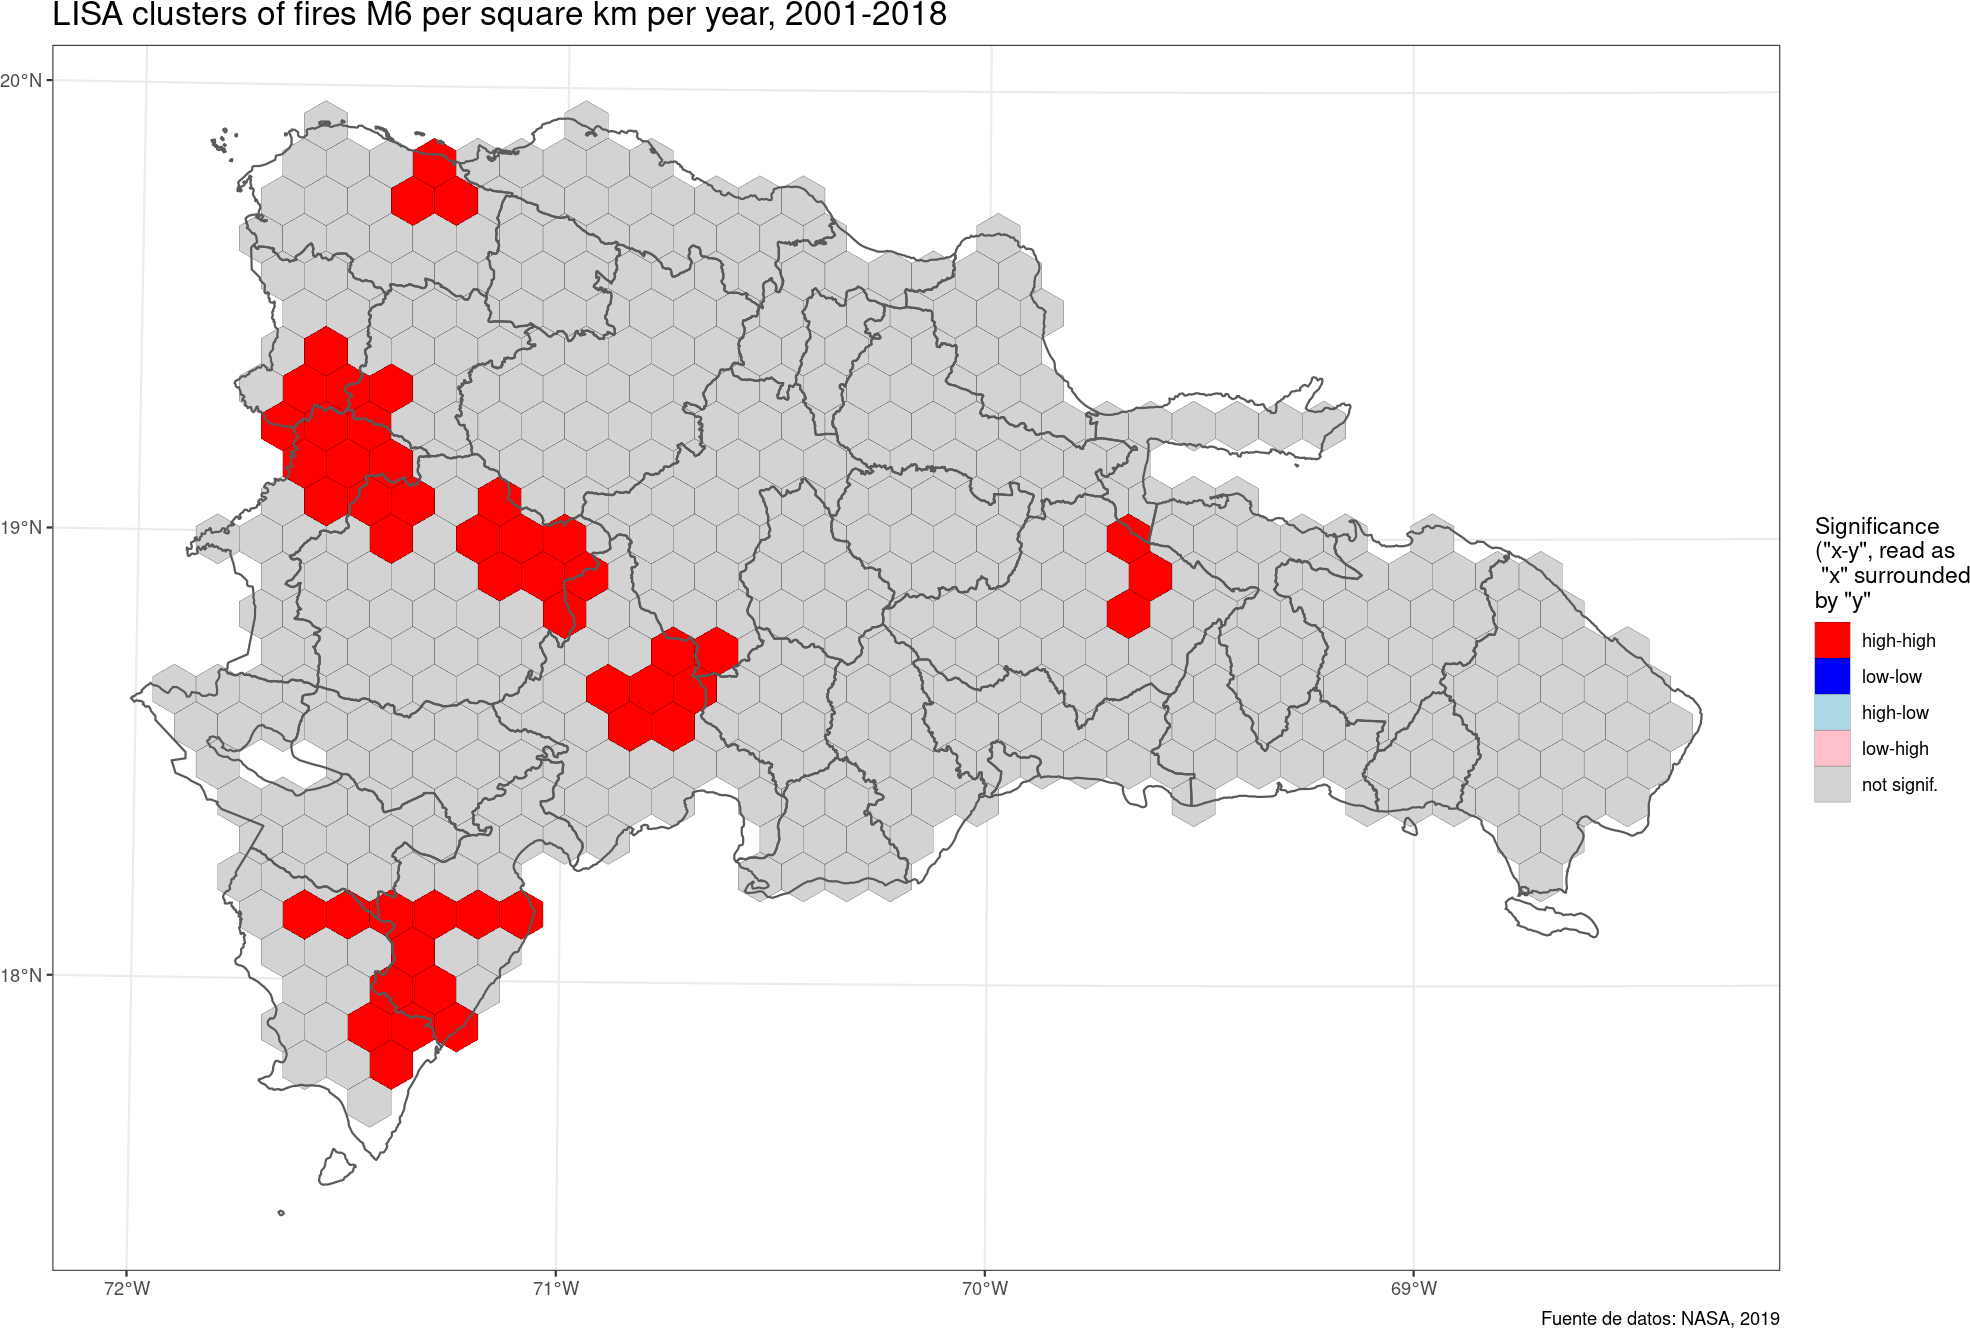
\includegraphics{img/modelling/lta-esda-9} \end{center}

\begin{Shaded}
\begin{Highlighting}[]

\CommentTok{\# * LISA Map LOSS1218\_PUA\_PYR\_NORM}
\NormalTok{grdlisamapl1218 }\OtherTok{\textless{}{-}} \FunctionTok{lisamap}\NormalTok{(}\AttributeTok{objesp =}\NormalTok{ grdzonal }\SpecialCharTok{\%\textgreater{}\%}
    \FunctionTok{replace}\NormalTok{(}\FunctionTok{is.na}\NormalTok{(.), }\DecValTok{0}\NormalTok{), }\AttributeTok{var =} \StringTok{"LOSS1218\_PUA\_PYR\_NORM"}\NormalTok{, }\AttributeTok{pesos =}\NormalTok{ grdww, }\AttributeTok{tituloleyenda =} \StringTok{"Significance}\SpecialCharTok{\textbackslash{}n}\StringTok{(}\SpecialCharTok{\textbackslash{}"}\StringTok{x{-}y}\SpecialCharTok{\textbackslash{}"}\StringTok{, read as}\SpecialCharTok{\textbackslash{}n}\StringTok{ }\SpecialCharTok{\textbackslash{}"}\StringTok{x}\SpecialCharTok{\textbackslash{}"}\StringTok{ surrounded}\SpecialCharTok{\textbackslash{}n}\StringTok{by }\SpecialCharTok{\textbackslash{}"}\StringTok{y}\SpecialCharTok{\textbackslash{}"}\StringTok{"}\NormalTok{,}
    \AttributeTok{leyenda =}\NormalTok{ T, }\AttributeTok{anchuratitulo =} \DecValTok{1000}\NormalTok{, }\AttributeTok{tamanotitulo =} \DecValTok{16}\NormalTok{, }\AttributeTok{fuentedatos =} \StringTok{"Hansen et al., 2013"}\NormalTok{,}
    \AttributeTok{titulomapa =} \FunctionTok{paste0}\NormalTok{(}\StringTok{"LISA clusters of forest loss per unit area per year, 2012{-}2018"}\NormalTok{))}
\NormalTok{grdlisamapl1218}\SpecialCharTok{$}\NormalTok{grafico}\SpecialCharTok{$}\NormalTok{layers }\OtherTok{\textless{}{-}} \FunctionTok{c}\NormalTok{(grdlisamapl1218}\SpecialCharTok{$}\NormalTok{grafico}\SpecialCharTok{$}\NormalTok{layers, }\FunctionTok{geom\_sf}\NormalTok{(}\AttributeTok{data =}\NormalTok{ prov,}
    \AttributeTok{fill =} \StringTok{"transparent"}\NormalTok{)[[}\DecValTok{1}\NormalTok{]])}
\NormalTok{grdlisamapl1218}\SpecialCharTok{$}\NormalTok{grafico}
\end{Highlighting}
\end{Shaded}

\begin{center}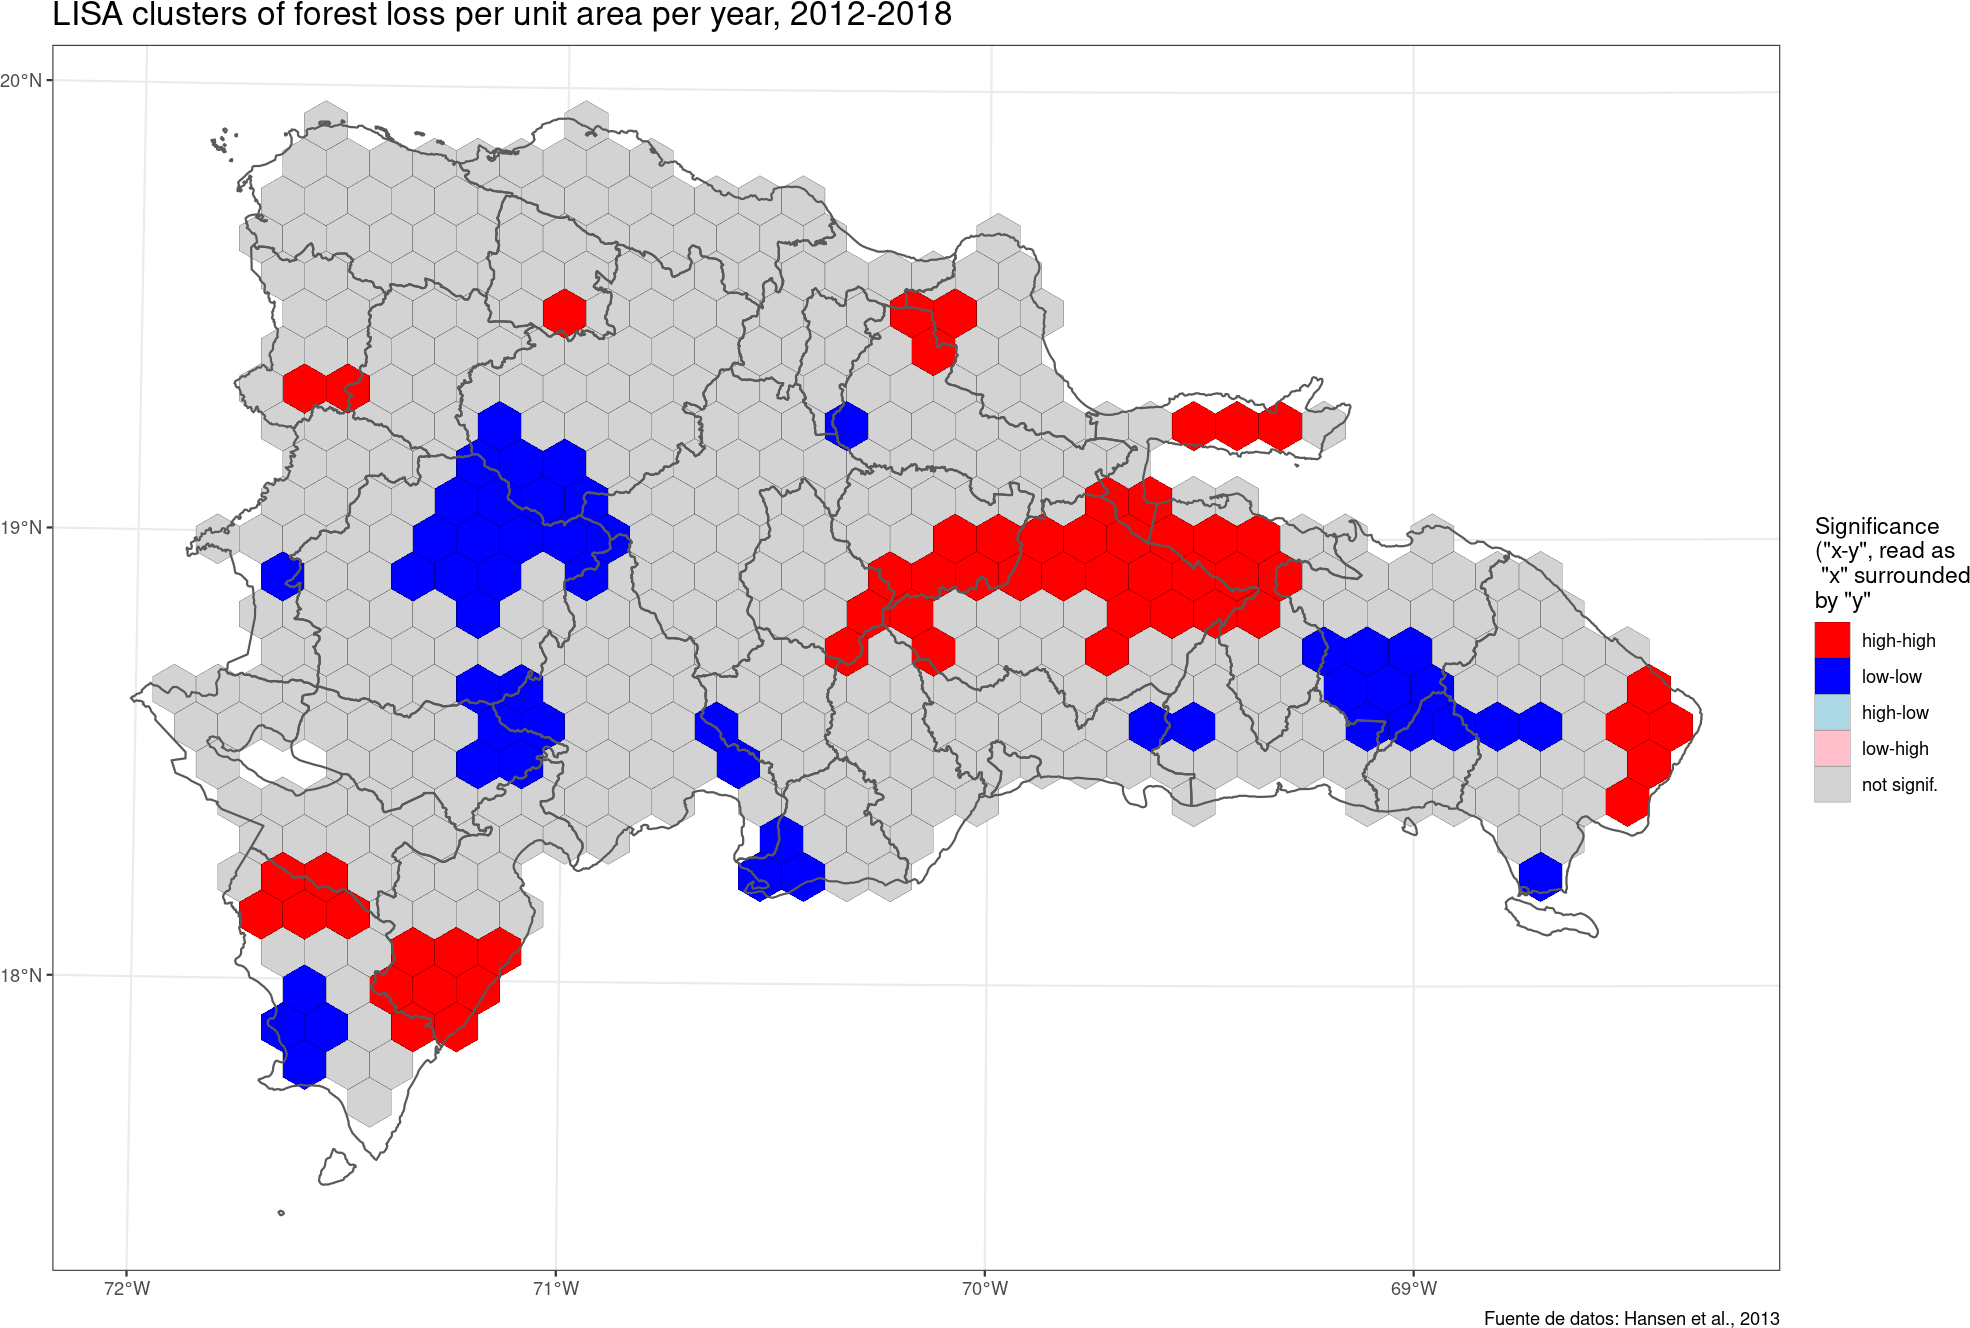
\includegraphics{img/modelling/lta-esda-10} \end{center}

\begin{Shaded}
\begin{Highlighting}[]

\CommentTok{\# * LISA Map FIRESV1\_PSQKM\_PYR per square km per year}
\NormalTok{grdlisamapfv1 }\OtherTok{\textless{}{-}} \FunctionTok{lisamap}\NormalTok{(}\AttributeTok{objesp =}\NormalTok{ grdzonal }\SpecialCharTok{\%\textgreater{}\%}
    \FunctionTok{replace}\NormalTok{(}\FunctionTok{is.na}\NormalTok{(.), }\DecValTok{0}\NormalTok{), }\AttributeTok{var =} \StringTok{"NFIRESV1\_PSQKM\_PYR"}\NormalTok{, }\AttributeTok{pesos =}\NormalTok{ grdww, }\AttributeTok{tituloleyenda =} \StringTok{"Significance}\SpecialCharTok{\textbackslash{}n}\StringTok{(}\SpecialCharTok{\textbackslash{}"}\StringTok{x{-}y}\SpecialCharTok{\textbackslash{}"}\StringTok{, read as}\SpecialCharTok{\textbackslash{}n}\StringTok{ }\SpecialCharTok{\textbackslash{}"}\StringTok{x}\SpecialCharTok{\textbackslash{}"}\StringTok{ surrounded}\SpecialCharTok{\textbackslash{}n}\StringTok{by }\SpecialCharTok{\textbackslash{}"}\StringTok{y}\SpecialCharTok{\textbackslash{}"}\StringTok{"}\NormalTok{,}
    \AttributeTok{leyenda =}\NormalTok{ T, }\AttributeTok{anchuratitulo =} \DecValTok{1000}\NormalTok{, }\AttributeTok{tamanotitulo =} \DecValTok{16}\NormalTok{, }\AttributeTok{fuentedatos =} \StringTok{"NASA, 2019"}\NormalTok{,}
    \AttributeTok{titulomapa =} \FunctionTok{paste0}\NormalTok{(}\StringTok{"LISA clusters of fires V1 per square km per year, 2012{-}2018"}\NormalTok{))}
\NormalTok{grdlisamapfv1}\SpecialCharTok{$}\NormalTok{grafico}\SpecialCharTok{$}\NormalTok{layers }\OtherTok{\textless{}{-}} \FunctionTok{c}\NormalTok{(grdlisamapfv1}\SpecialCharTok{$}\NormalTok{grafico}\SpecialCharTok{$}\NormalTok{layers, }\FunctionTok{geom\_sf}\NormalTok{(}\AttributeTok{data =}\NormalTok{ prov,}
    \AttributeTok{fill =} \StringTok{"transparent"}\NormalTok{)[[}\DecValTok{1}\NormalTok{]])}
\NormalTok{grdlisamapfv1}\SpecialCharTok{$}\NormalTok{grafico}
\end{Highlighting}
\end{Shaded}

\begin{center}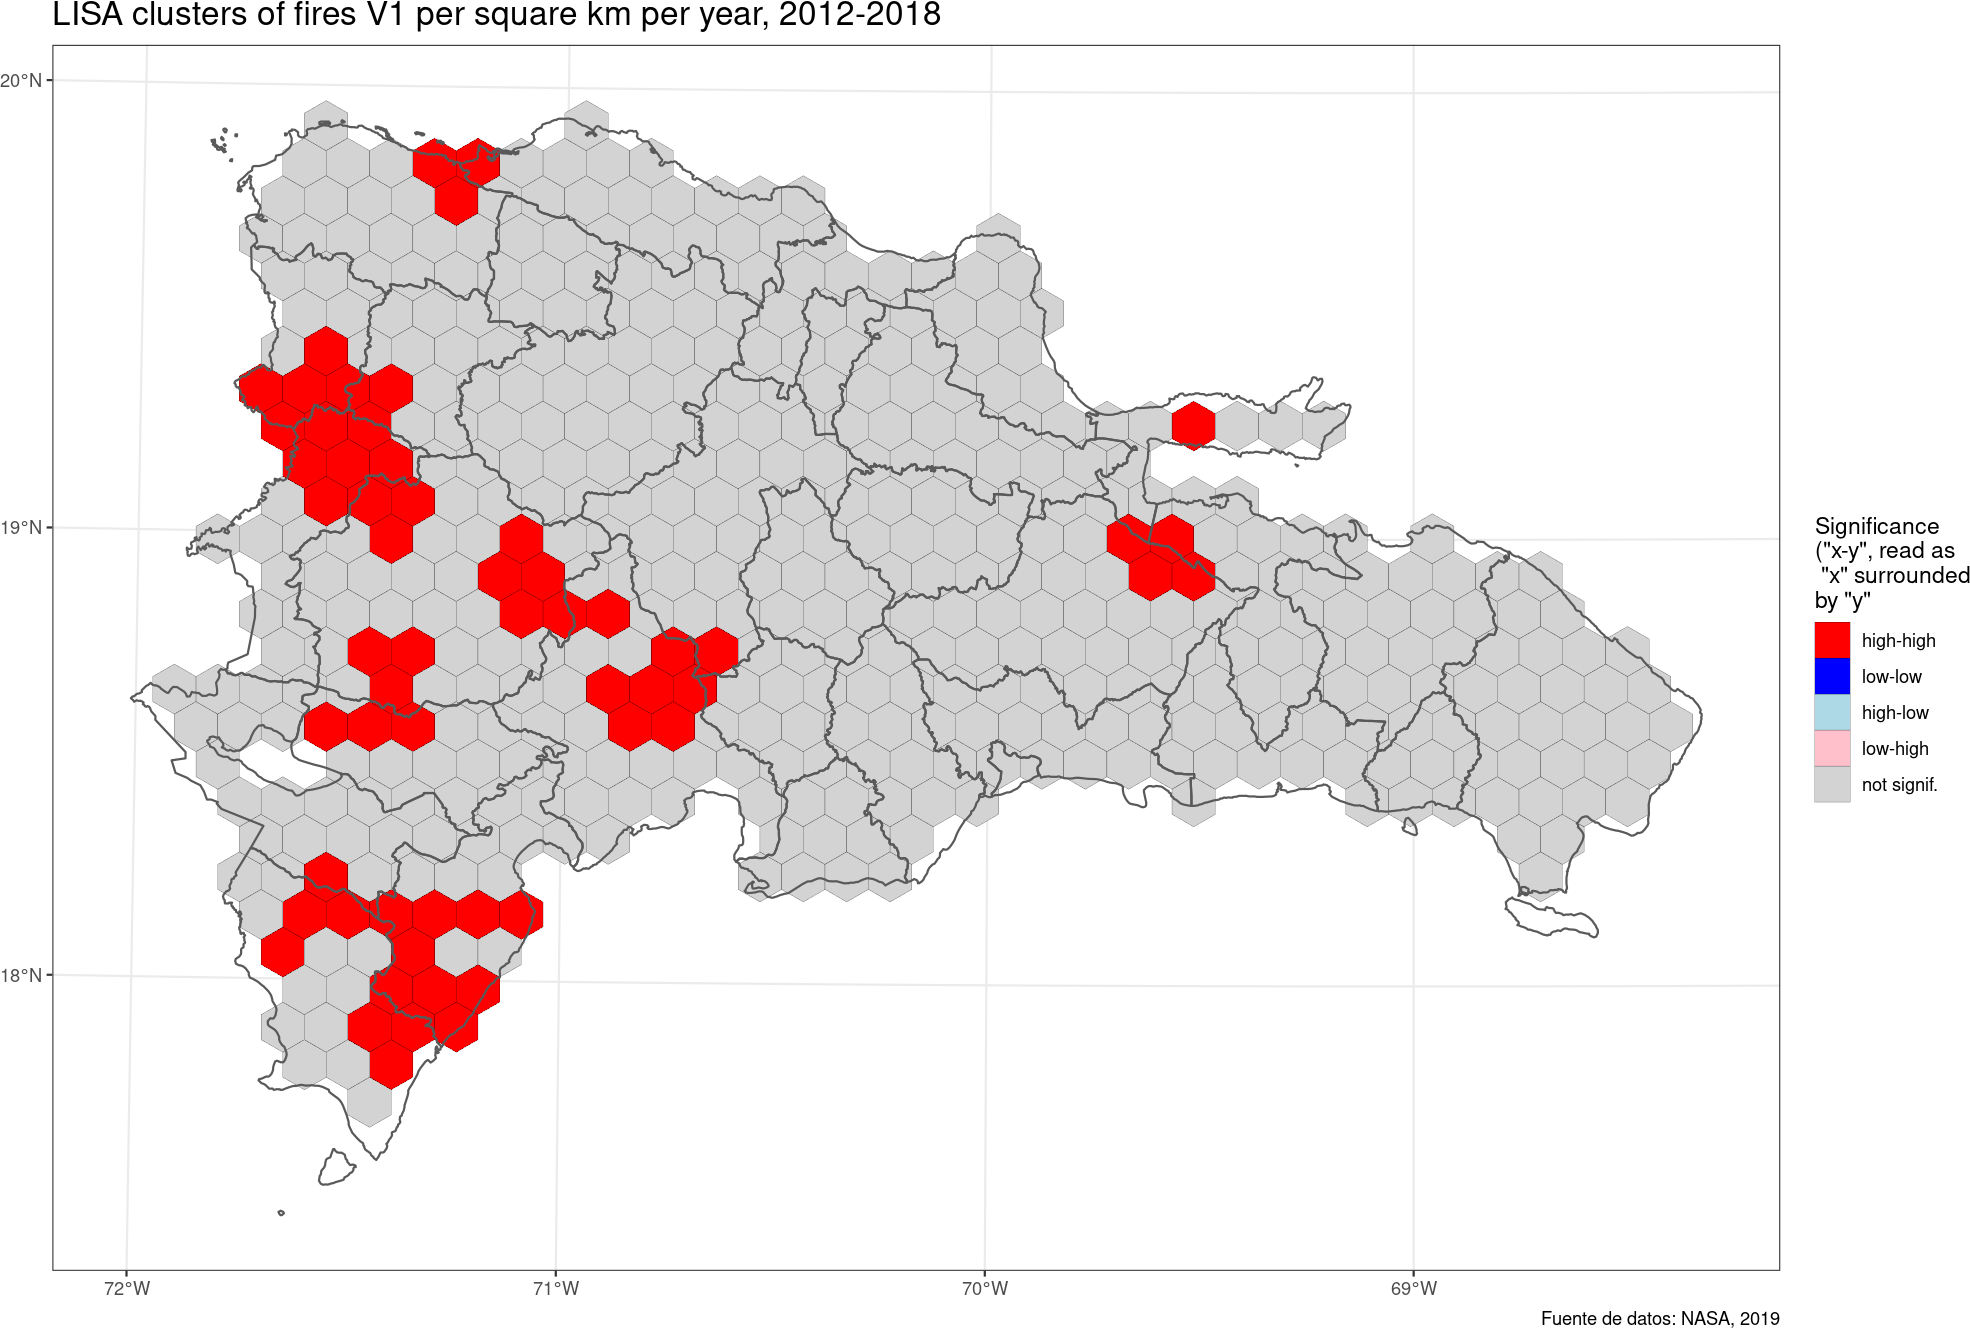
\includegraphics{img/modelling/lta-esda-11} \end{center}

\begin{Shaded}
\begin{Highlighting}[]

\CommentTok{\# * LISA Map FIRESV1\_PSQKM\_PYR\_TLP per square km per year}
\NormalTok{grdlisamapfv1tlp }\OtherTok{\textless{}{-}} \FunctionTok{lisamap}\NormalTok{(}\AttributeTok{objesp =}\NormalTok{ grdzonal }\SpecialCharTok{\%\textgreater{}\%}
    \FunctionTok{replace}\NormalTok{(}\FunctionTok{is.na}\NormalTok{(.), }\DecValTok{0}\NormalTok{), }\AttributeTok{var =} \StringTok{"NFIRESV1\_PSQKM\_PYR\_TLP"}\NormalTok{, }\AttributeTok{pesos =}\NormalTok{ grdww, }\AttributeTok{tituloleyenda =} \StringTok{"Significance}\SpecialCharTok{\textbackslash{}n}\StringTok{(}\SpecialCharTok{\textbackslash{}"}\StringTok{x{-}y}\SpecialCharTok{\textbackslash{}"}\StringTok{, read as}\SpecialCharTok{\textbackslash{}n}\StringTok{ }\SpecialCharTok{\textbackslash{}"}\StringTok{x}\SpecialCharTok{\textbackslash{}"}\StringTok{ surrounded}\SpecialCharTok{\textbackslash{}n}\StringTok{by }\SpecialCharTok{\textbackslash{}"}\StringTok{y}\SpecialCharTok{\textbackslash{}"}\StringTok{"}\NormalTok{,}
    \AttributeTok{leyenda =}\NormalTok{ T, }\AttributeTok{anchuratitulo =} \DecValTok{1000}\NormalTok{, }\AttributeTok{tamanotitulo =} \DecValTok{16}\NormalTok{, }\AttributeTok{fuentedatos =} \StringTok{"NASA, 2019"}\NormalTok{,}
    \AttributeTok{titulomapa =} \FunctionTok{paste0}\NormalTok{(}\StringTok{"LISA clusters of fires V1 (transformed) per square km per year, 2012{-}2018"}\NormalTok{))}
\NormalTok{grdlisamapfv1tlp}\SpecialCharTok{$}\NormalTok{grafico}\SpecialCharTok{$}\NormalTok{layers }\OtherTok{\textless{}{-}} \FunctionTok{c}\NormalTok{(grdlisamapfv1tlp}\SpecialCharTok{$}\NormalTok{grafico}\SpecialCharTok{$}\NormalTok{layers, }\FunctionTok{geom\_sf}\NormalTok{(}\AttributeTok{data =}\NormalTok{ prov,}
    \AttributeTok{fill =} \StringTok{"transparent"}\NormalTok{)[[}\DecValTok{1}\NormalTok{]])}
\NormalTok{grdlisamapfv1tlp}\SpecialCharTok{$}\NormalTok{grafico}
\end{Highlighting}
\end{Shaded}

\begin{center}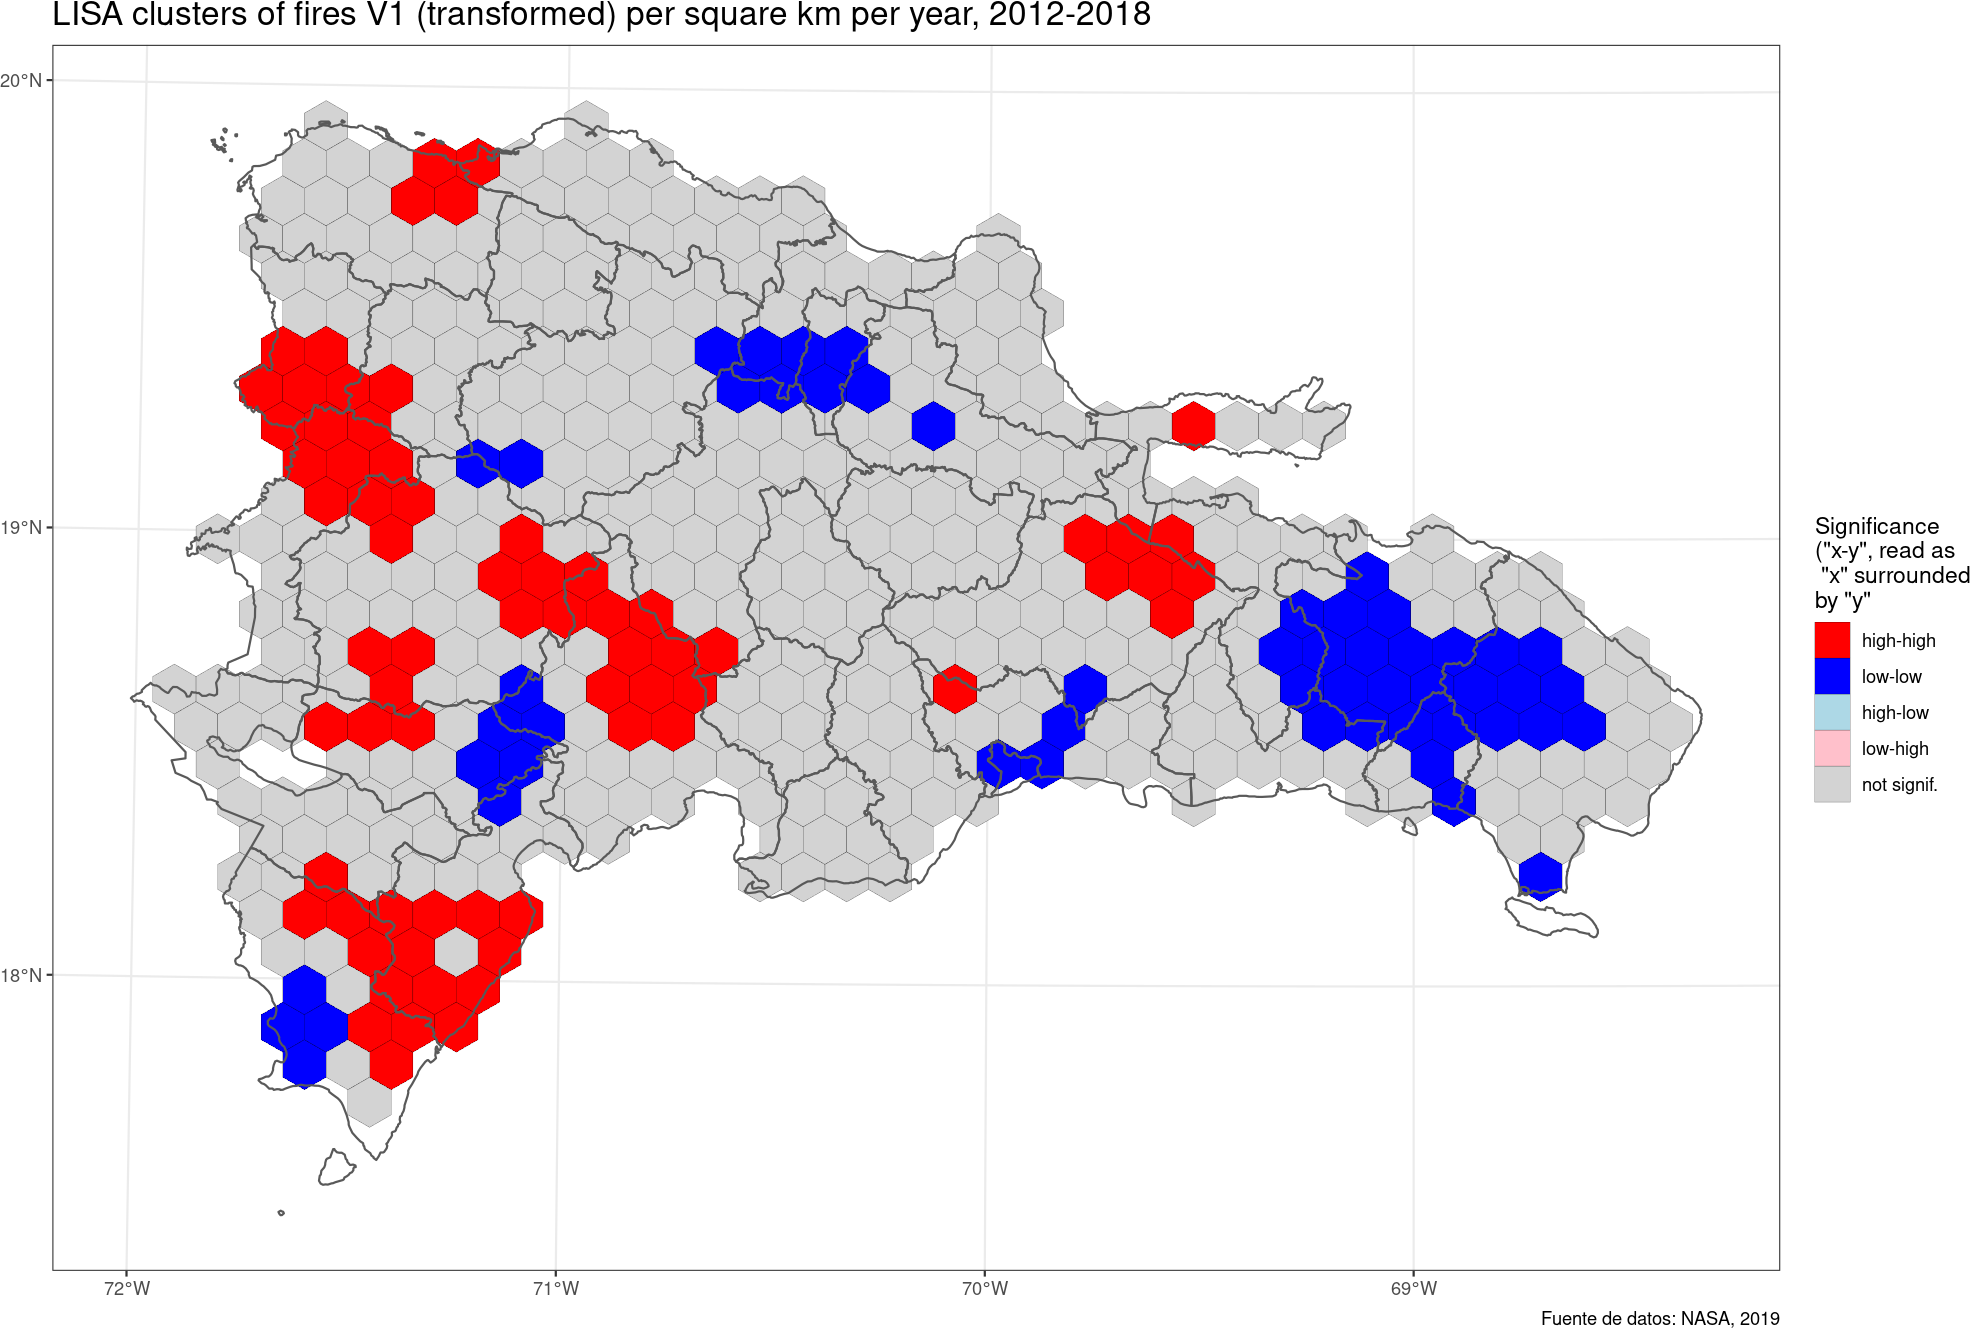
\includegraphics{img/modelling/lta-esda-12} \end{center}

\begin{Shaded}
\begin{Highlighting}[]

\CommentTok{\# * LISA Map FIRESM6\_PSQKM\_PYR\_TLP per square km per year \{tmap\} (for}
\CommentTok{\# manuscript)}
\NormalTok{grdlisamapl0118\_obj }\OtherTok{\textless{}{-}} \FunctionTok{lisamap\_tmap\_obj}\NormalTok{(}\AttributeTok{objesp =}\NormalTok{ grdzonal }\SpecialCharTok{\%\textgreater{}\%}
    \FunctionTok{replace}\NormalTok{(}\FunctionTok{is.na}\NormalTok{(.), }\DecValTok{0}\NormalTok{), }\AttributeTok{var =} \StringTok{"LOSS0118\_PUA\_PYR\_NORM"}\NormalTok{, }\AttributeTok{pesos =}\NormalTok{ grdww)}
\NormalTok{grdlisamapl1218\_obj }\OtherTok{\textless{}{-}} \FunctionTok{lisamap\_tmap\_obj}\NormalTok{(}\AttributeTok{objesp =}\NormalTok{ grdzonal }\SpecialCharTok{\%\textgreater{}\%}
    \FunctionTok{replace}\NormalTok{(}\FunctionTok{is.na}\NormalTok{(.), }\DecValTok{0}\NormalTok{), }\AttributeTok{var =} \StringTok{"LOSS1218\_PUA\_PYR\_NORM"}\NormalTok{, }\AttributeTok{pesos =}\NormalTok{ grdww)}
\NormalTok{grdlisamapfm6tlp\_obj }\OtherTok{\textless{}{-}} \FunctionTok{lisamap\_tmap\_obj}\NormalTok{(}\AttributeTok{objesp =}\NormalTok{ grdzonal }\SpecialCharTok{\%\textgreater{}\%}
    \FunctionTok{replace}\NormalTok{(}\FunctionTok{is.na}\NormalTok{(.), }\DecValTok{0}\NormalTok{), }\AttributeTok{var =} \StringTok{"NFIRESM6\_PSQKM\_PYR\_TLP"}\NormalTok{, }\AttributeTok{pesos =}\NormalTok{ grdww)}
\NormalTok{grdlisamapfv1tlp\_obj }\OtherTok{\textless{}{-}} \FunctionTok{lisamap\_tmap\_obj}\NormalTok{(}\AttributeTok{objesp =}\NormalTok{ grdzonal }\SpecialCharTok{\%\textgreater{}\%}
    \FunctionTok{replace}\NormalTok{(}\FunctionTok{is.na}\NormalTok{(.), }\DecValTok{0}\NormalTok{), }\AttributeTok{var =} \StringTok{"NFIRESV1\_PSQKM\_PYR\_TLP"}\NormalTok{, }\AttributeTok{pesos =}\NormalTok{ grdww)}

\NormalTok{grdlisamap\_objs }\OtherTok{\textless{}{-}}\NormalTok{ grdlisamapl0118\_obj }\SpecialCharTok{\%\textgreater{}\%}
    \FunctionTok{select}\NormalTok{(}\SpecialCharTok{{-}}\NormalTok{LOSS0118\_PUA\_PYR\_NORM) }\SpecialCharTok{\%\textgreater{}\%}
    \FunctionTok{inner\_join}\NormalTok{(}\FunctionTok{Reduce}\NormalTok{(}\ControlFlowTok{function}\NormalTok{(...) }\FunctionTok{merge}\NormalTok{(..., }\AttributeTok{by =} \StringTok{"ENLACE"}\NormalTok{, }\AttributeTok{all.x =} \ConstantTok{TRUE}\NormalTok{), }\FunctionTok{list}\NormalTok{(grdlisamapl0118\_obj }\SpecialCharTok{\%\textgreater{}\%}
        \FunctionTok{st\_drop\_geometry}\NormalTok{(), grdlisamapl1218\_obj }\SpecialCharTok{\%\textgreater{}\%}
        \FunctionTok{st\_drop\_geometry}\NormalTok{(), grdlisamapfm6tlp\_obj }\SpecialCharTok{\%\textgreater{}\%}
        \FunctionTok{st\_drop\_geometry}\NormalTok{(), grdlisamapfv1tlp\_obj }\SpecialCharTok{\%\textgreater{}\%}
        \FunctionTok{st\_drop\_geometry}\NormalTok{())), }\AttributeTok{by =} \StringTok{"ENLACE"}\NormalTok{)}
\CommentTok{\# jpeg(\textquotesingle{}out/lisamaps\_loss0118\_loss1218\_firesm6\_firesv1.jpg\textquotesingle{}, width = 3840,}
\CommentTok{\# height = 2160, res = 250)}
\NormalTok{\{}
\NormalTok{    grdlisamap\_objs }\SpecialCharTok{\%\textgreater{}\%}
\NormalTok{        dplyr}\SpecialCharTok{::}\FunctionTok{select}\NormalTok{(}\StringTok{\textasciigrave{}}\AttributeTok{(A)}\StringTok{\textasciigrave{}} \OtherTok{=}\NormalTok{ LOSS0118\_PUA\_PYR\_NORM, }\StringTok{\textasciigrave{}}\AttributeTok{(B)}\StringTok{\textasciigrave{}} \OtherTok{=}\NormalTok{ LOSS1218\_PUA\_PYR\_NORM,}
            \StringTok{\textasciigrave{}}\AttributeTok{(C)}\StringTok{\textasciigrave{}} \OtherTok{=}\NormalTok{ NFIRESM6\_PSQKM\_PYR\_TLP, }\StringTok{\textasciigrave{}}\AttributeTok{(D)}\StringTok{\textasciigrave{}} \OtherTok{=}\NormalTok{ NFIRESV1\_PSQKM\_PYR\_TLP) }\SpecialCharTok{\%\textgreater{}\%}
        \FunctionTok{replace}\NormalTok{(}\FunctionTok{is.na}\NormalTok{(.), }\DecValTok{0}\NormalTok{) }\SpecialCharTok{\%\textgreater{}\%}
        \FunctionTok{gather}\NormalTok{(variable, value, }\SpecialCharTok{{-}}\NormalTok{geometry) }\SpecialCharTok{\%\textgreater{}\%}
        \FunctionTok{mutate}\NormalTok{(}\AttributeTok{variable =} \FunctionTok{factor}\NormalTok{(variable, }\AttributeTok{levels =} \FunctionTok{unique}\NormalTok{(variable))) }\SpecialCharTok{\%\textgreater{}\%}
        \FunctionTok{mutate}\NormalTok{(}\AttributeTok{color =} \FunctionTok{case\_when}\NormalTok{(value }\SpecialCharTok{==} \StringTok{"high{-}high"} \SpecialCharTok{\textasciitilde{}} \StringTok{"red"}\NormalTok{, value }\SpecialCharTok{==} \StringTok{"low{-}low"} \SpecialCharTok{\textasciitilde{}}
            \StringTok{"blue"}\NormalTok{, value }\SpecialCharTok{==} \StringTok{"high{-}low"} \SpecialCharTok{\textasciitilde{}} \StringTok{"lightblue"}\NormalTok{, value }\SpecialCharTok{==} \StringTok{"low{-}high"} \SpecialCharTok{\textasciitilde{}} \StringTok{"pink"}\NormalTok{,}
\NormalTok{            value }\SpecialCharTok{==} \StringTok{"not signif."} \SpecialCharTok{\textasciitilde{}} \StringTok{"lightgrey"}\NormalTok{)) }\SpecialCharTok{\%\textgreater{}\%}
        \FunctionTok{tm\_shape}\NormalTok{() }\SpecialCharTok{+} \FunctionTok{tm\_fill}\NormalTok{(}\AttributeTok{col =} \StringTok{"color"}\NormalTok{, }\AttributeTok{size =} \FloatTok{0.1}\NormalTok{, }\AttributeTok{legend.is.portrait =}\NormalTok{ T, }\AttributeTok{legend.format =} \FunctionTok{list}\NormalTok{(}\AttributeTok{digits =} \DecValTok{2}\NormalTok{,}
        \AttributeTok{text.separator =} \StringTok{"{-}"}\NormalTok{)) }\SpecialCharTok{+} \FunctionTok{tm\_borders}\NormalTok{(}\AttributeTok{col =} \StringTok{"grey15"}\NormalTok{, }\AttributeTok{lwd =} \FloatTok{0.3}\NormalTok{) }\SpecialCharTok{+} \FunctionTok{tm\_facets}\NormalTok{(}\AttributeTok{by =} \StringTok{"variable"}\NormalTok{,}
        \AttributeTok{nrow =} \DecValTok{2}\NormalTok{, }\AttributeTok{free.coords =} \ConstantTok{FALSE}\NormalTok{, }\AttributeTok{free.scales =} \ConstantTok{TRUE}\NormalTok{) }\SpecialCharTok{+} \FunctionTok{tm\_layout}\NormalTok{(}\AttributeTok{panel.label.size =} \DecValTok{3}\NormalTok{,}
        \AttributeTok{legend.title.size =} \FloatTok{1e{-}04}\NormalTok{, }\AttributeTok{legend.text.size =} \FloatTok{1.8}\NormalTok{, }\AttributeTok{bg.color =} \StringTok{"white"}\NormalTok{, }\AttributeTok{legend.format =} \FunctionTok{list}\NormalTok{(}\AttributeTok{fun =} \ControlFlowTok{function}\NormalTok{(x) }\FunctionTok{formatC}\NormalTok{(x,}
            \AttributeTok{digits =} \DecValTok{2}\NormalTok{, }\AttributeTok{format =} \StringTok{"f"}\NormalTok{))) }\SpecialCharTok{+} \FunctionTok{tm\_shape}\NormalTok{(seaocean) }\SpecialCharTok{+} \FunctionTok{tm\_borders}\NormalTok{() }\SpecialCharTok{+} \FunctionTok{tm\_fill}\NormalTok{(}\AttributeTok{col =} \StringTok{"white"}\NormalTok{)  }\CommentTok{\#+ }
    \CommentTok{\# tm\_shape(points\_of\_interest) + tm\_text(\textquotesingle{}code\textquotesingle{}, size = 2, col = \textquotesingle{}black\textquotesingle{},}
    \CommentTok{\# fontface = \textquotesingle{}bold\textquotesingle{}, bg.color = \textquotesingle{}white\textquotesingle{}, bg.alpha = 0.5)}
\NormalTok{\}}
\end{Highlighting}
\end{Shaded}

\begin{center}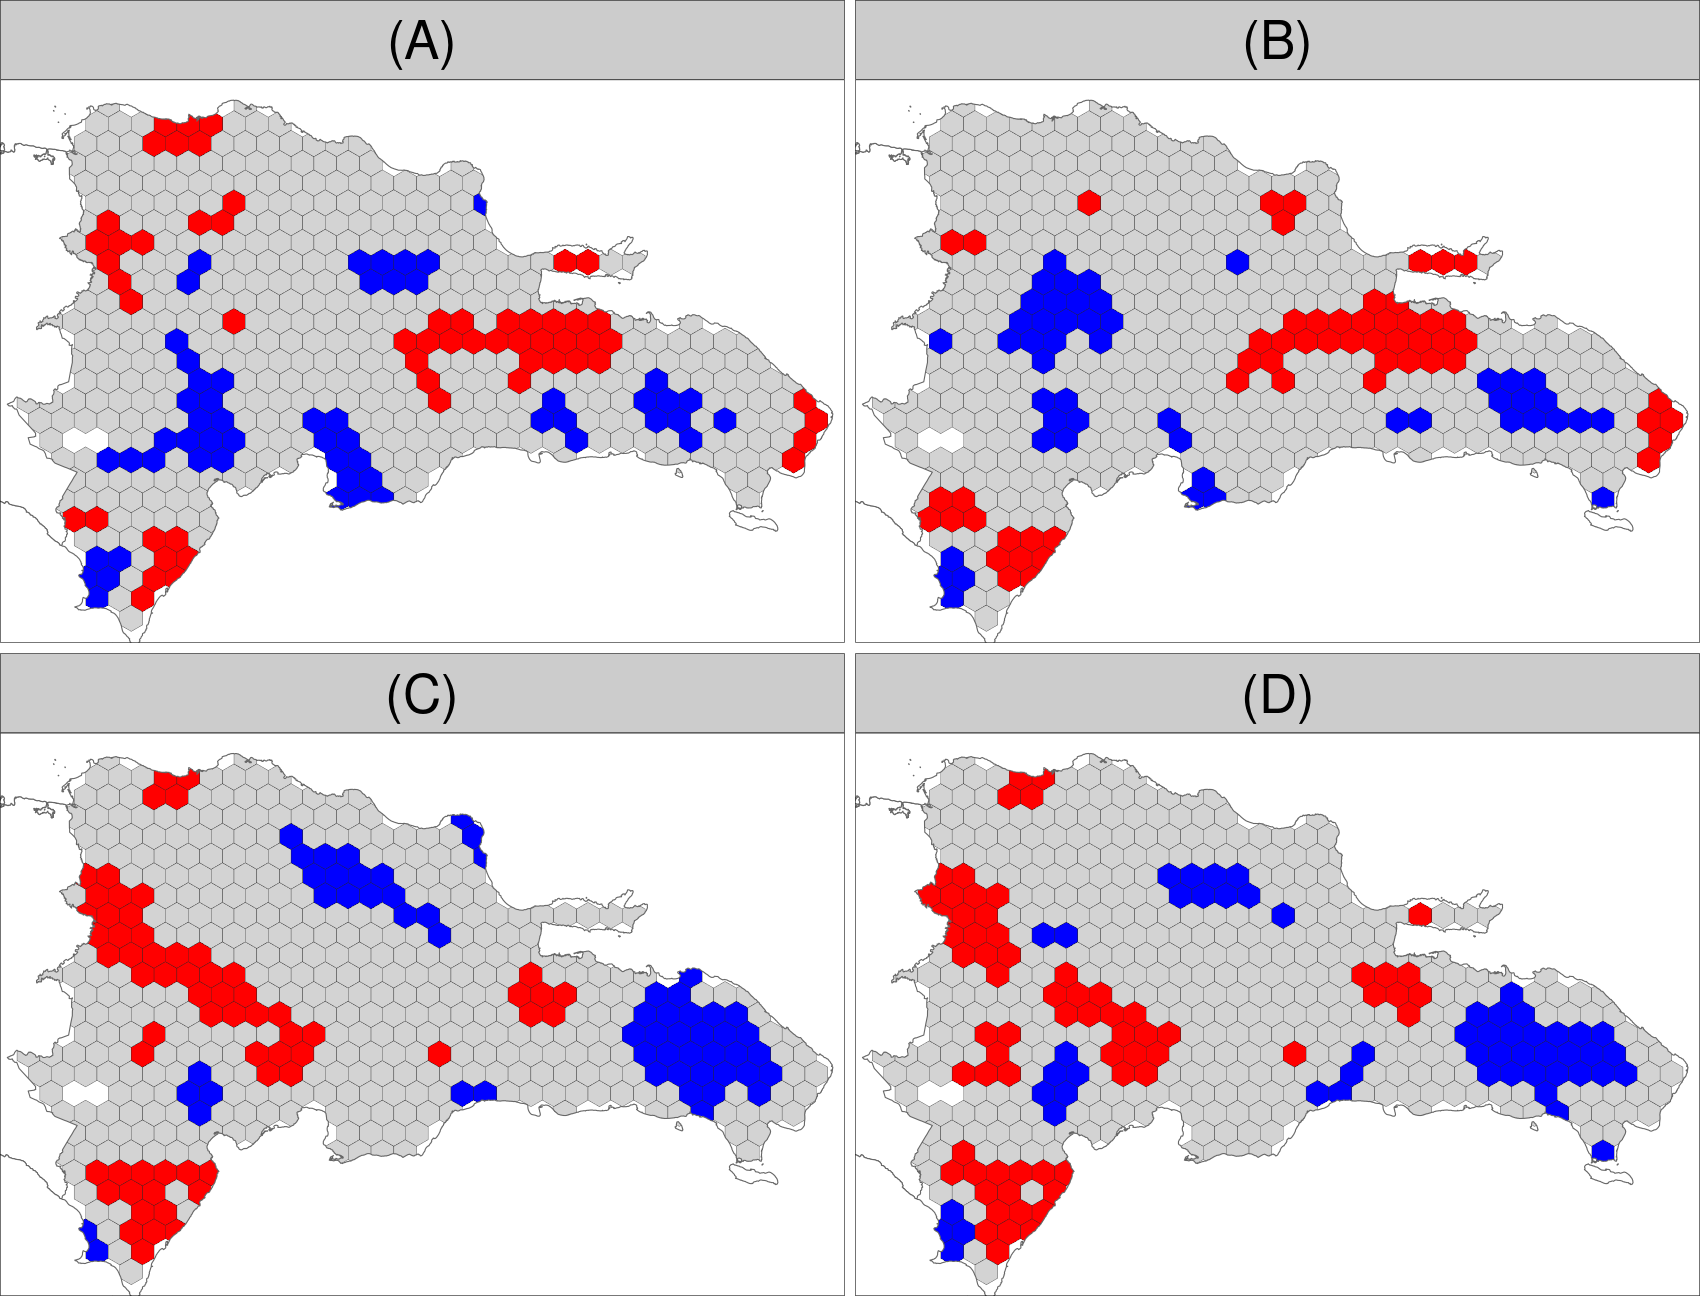
\includegraphics{img/modelling/lta-esda-13} \end{center}

\begin{Shaded}
\begin{Highlighting}[]
\CommentTok{\# dev.off()}

\CommentTok{\# Statistical summaries}
\NormalTok{grdzonaledam6 }\OtherTok{\textless{}{-}}\NormalTok{ grdzonal }\SpecialCharTok{\%\textgreater{}\%}
    \FunctionTok{mutate}\NormalTok{(}\AttributeTok{LOSS0118\_AREASQKM =}\NormalTok{ LOSS0118\_AREASQM}\SpecialCharTok{/}\FloatTok{1e+06}\NormalTok{) }\SpecialCharTok{\%\textgreater{}\%}
\NormalTok{    dplyr}\SpecialCharTok{::}\FunctionTok{select}\NormalTok{(ENLACE, NFIRESM6, NFIRESM6\_PSQKM, NFIRESM6\_PSQKM\_PYR, NFIRESM6\_PSQKM\_PYR\_TLP,}
\NormalTok{        LOSS0118\_AREASQKM, LOSS0118\_PUA, LOSS0118\_PUA\_PYR, LOSS0118\_PUA\_PYR\_NORM) }\SpecialCharTok{\%\textgreater{}\%}
    \FunctionTok{replace}\NormalTok{(}\FunctionTok{is.na}\NormalTok{(.), }\DecValTok{0}\NormalTok{)}

\NormalTok{grdzonaledav1 }\OtherTok{\textless{}{-}}\NormalTok{ grdzonal }\SpecialCharTok{\%\textgreater{}\%}
    \FunctionTok{mutate}\NormalTok{(}\AttributeTok{LOSS1218\_AREASQKM =}\NormalTok{ LOSS1218\_AREASQM}\SpecialCharTok{/}\FloatTok{1e+06}\NormalTok{) }\SpecialCharTok{\%\textgreater{}\%}
\NormalTok{    dplyr}\SpecialCharTok{::}\FunctionTok{select}\NormalTok{(ENLACE, NFIRESV1, NFIRESV1\_PSQKM, NFIRESV1\_PSQKM\_PYR, NFIRESV1\_PSQKM\_PYR\_TLP,}
\NormalTok{        LOSS1218\_AREASQKM, LOSS1218\_PUA, LOSS1218\_PUA\_PYR, LOSS1218\_PUA\_PYR\_NORM) }\SpecialCharTok{\%\textgreater{}\%}
    \FunctionTok{replace}\NormalTok{(}\FunctionTok{is.na}\NormalTok{(.), }\DecValTok{0}\NormalTok{)}
\CommentTok{\# Statistical summaries (latex table for manuscript)}
\NormalTok{grdzonaledam6 }\SpecialCharTok{\%\textgreater{}\%}
\NormalTok{    st\_drop\_geometry }\SpecialCharTok{\%\textgreater{}\%}
    \FunctionTok{gather}\NormalTok{(key, val) }\SpecialCharTok{\%\textgreater{}\%}
    \FunctionTok{distinct}\NormalTok{(key)}
\DocumentationTok{\#\#                      key}
\DocumentationTok{\#\# 1                 ENLACE}
\DocumentationTok{\#\# 2               NFIRESM6}
\DocumentationTok{\#\# 3         NFIRESM6\_PSQKM}
\DocumentationTok{\#\# 4     NFIRESM6\_PSQKM\_PYR}
\DocumentationTok{\#\# 5 NFIRESM6\_PSQKM\_PYR\_TLP}
\DocumentationTok{\#\# 6      LOSS0118\_AREASQKM}
\DocumentationTok{\#\# 7           LOSS0118\_PUA}
\DocumentationTok{\#\# 8       LOSS0118\_PUA\_PYR}
\DocumentationTok{\#\# 9  LOSS0118\_PUA\_PYR\_NORM}
\NormalTok{grdzonaledam6 }\SpecialCharTok{\%\textgreater{}\%}
\NormalTok{    st\_drop\_geometry }\SpecialCharTok{\%\textgreater{}\%}
    \FunctionTok{summarise}\NormalTok{(}\StringTok{\textasciigrave{}}\AttributeTok{Total number of fire points}\StringTok{\textasciigrave{}} \OtherTok{=} \FunctionTok{sum}\NormalTok{(NFIRESM6), }\StringTok{\textasciigrave{}}\AttributeTok{Average number of fire points per 100 sq. km}\StringTok{\textasciigrave{}} \OtherTok{=} \FunctionTok{mean}\NormalTok{(NFIRESM6\_PSQKM) }\SpecialCharTok{*}
        \DecValTok{100}\NormalTok{, }\StringTok{\textasciigrave{}}\AttributeTok{Average number of fire points per 100 sq. km per year}\StringTok{\textasciigrave{}} \OtherTok{=} \FunctionTok{mean}\NormalTok{(NFIRESM6\_PSQKM\_PYR) }\SpecialCharTok{*}
        \DecValTok{100}\NormalTok{, }\StringTok{\textasciigrave{}}\AttributeTok{Maximum number of fire points per 100 sq. km per year}\StringTok{\textasciigrave{}} \OtherTok{=} \FunctionTok{max}\NormalTok{(NFIRESM6\_PSQKM\_PYR) }\SpecialCharTok{*}
        \DecValTok{100}\NormalTok{, }\StringTok{\textasciigrave{}}\AttributeTok{Total forest loss area (sq. km)}\StringTok{\textasciigrave{}} \OtherTok{=} \FunctionTok{sum}\NormalTok{(LOSS0118\_AREASQKM), }\StringTok{\textasciigrave{}}\AttributeTok{Average forest loss area (sq. km) per 100 sq. km}\StringTok{\textasciigrave{}} \OtherTok{=} \FunctionTok{mean}\NormalTok{(LOSS0118\_PUA) }\SpecialCharTok{*}
        \DecValTok{100}\NormalTok{, }\StringTok{\textasciigrave{}}\AttributeTok{Average forest loss area (sq. km) per 100 sq. km per year}\StringTok{\textasciigrave{}} \OtherTok{=} \FunctionTok{mean}\NormalTok{(LOSS0118\_PUA\_PYR) }\SpecialCharTok{*}
        \DecValTok{100}\NormalTok{, }\StringTok{\textasciigrave{}}\AttributeTok{Maximum forest loss area (sq. km) per 100 sq. km per year}\StringTok{\textasciigrave{}} \OtherTok{=} \FunctionTok{max}\NormalTok{(LOSS0118\_PUA\_PYR) }\SpecialCharTok{*}
        \DecValTok{100}\NormalTok{) }\SpecialCharTok{\%\textgreater{}\%}
    \FunctionTok{gather}\NormalTok{(Attribute, }\StringTok{\textasciigrave{}}\AttributeTok{Period 2001{-}2018, MODIS fire points}\StringTok{\textasciigrave{}}\NormalTok{) }\SpecialCharTok{\%\textgreater{}\%}
    \FunctionTok{inner\_join}\NormalTok{(grdzonaledav1 }\SpecialCharTok{\%\textgreater{}\%}
\NormalTok{        st\_drop\_geometry }\SpecialCharTok{\%\textgreater{}\%}
        \FunctionTok{summarise}\NormalTok{(}\StringTok{\textasciigrave{}}\AttributeTok{Total number of fire points}\StringTok{\textasciigrave{}} \OtherTok{=} \FunctionTok{sum}\NormalTok{(NFIRESV1), }\StringTok{\textasciigrave{}}\AttributeTok{Average number of fire points per 100 sq. km}\StringTok{\textasciigrave{}} \OtherTok{=} \FunctionTok{mean}\NormalTok{(NFIRESV1\_PSQKM) }\SpecialCharTok{*}
            \DecValTok{100}\NormalTok{, }\StringTok{\textasciigrave{}}\AttributeTok{Average number of fire points per 100 sq. km per year}\StringTok{\textasciigrave{}} \OtherTok{=} \FunctionTok{mean}\NormalTok{(NFIRESV1\_PSQKM\_PYR) }\SpecialCharTok{*}
            \DecValTok{100}\NormalTok{, }\StringTok{\textasciigrave{}}\AttributeTok{Maximum number of fire points per 100 sq. km per year}\StringTok{\textasciigrave{}} \OtherTok{=} \FunctionTok{max}\NormalTok{(NFIRESV1\_PSQKM\_PYR) }\SpecialCharTok{*}
            \DecValTok{100}\NormalTok{, }\StringTok{\textasciigrave{}}\AttributeTok{Total forest loss area (sq. km)}\StringTok{\textasciigrave{}} \OtherTok{=} \FunctionTok{sum}\NormalTok{(LOSS1218\_AREASQKM), }\StringTok{\textasciigrave{}}\AttributeTok{Average forest loss area (sq. km) per 100 sq. km}\StringTok{\textasciigrave{}} \OtherTok{=} \FunctionTok{mean}\NormalTok{(LOSS1218\_PUA) }\SpecialCharTok{*}
            \DecValTok{100}\NormalTok{, }\StringTok{\textasciigrave{}}\AttributeTok{Average forest loss area (sq. km) per 100 sq. km per year}\StringTok{\textasciigrave{}} \OtherTok{=} \FunctionTok{mean}\NormalTok{(LOSS1218\_PUA\_PYR) }\SpecialCharTok{*}
            \DecValTok{100}\NormalTok{, }\StringTok{\textasciigrave{}}\AttributeTok{Maximum forest loss area (sq. km) per 100 sq. km per year}\StringTok{\textasciigrave{}} \OtherTok{=} \FunctionTok{max}\NormalTok{(LOSS1218\_PUA\_PYR) }\SpecialCharTok{*}
            \DecValTok{100}\NormalTok{) }\SpecialCharTok{\%\textgreater{}\%}
        \FunctionTok{gather}\NormalTok{(Attribute, }\StringTok{\textasciigrave{}}\AttributeTok{Period 2012{-}2018, VIIRS fire points}\StringTok{\textasciigrave{}}\NormalTok{)) }\SpecialCharTok{\%\textgreater{}\%}
    \FunctionTok{mutate\_if}\NormalTok{(is.numeric, round, }\DecValTok{2}\NormalTok{) }\SpecialCharTok{\%\textgreater{}\%}
    \FunctionTok{mutate\_if}\NormalTok{(is.numeric, as.character) }\SpecialCharTok{\%\textgreater{}\%}
\NormalTok{    knitr}\SpecialCharTok{::}\FunctionTok{kable}\NormalTok{(}\AttributeTok{format =} \StringTok{"latex"}\NormalTok{, }\AttributeTok{digits =} \DecValTok{2}\NormalTok{)}
\end{Highlighting}
\end{Shaded}

\begin{tabular}{l|l|l}
\hline
Attribute & Period 2001-2018, MODIS fire points & Period 2012-2018, VIIRS fire points\\
\hline
Total number of fire points & 11666 & 25231\\
\hline
Average number of fire points per 100 sq. km & 25.13 & 54.86\\
\hline
Average number of fire points per 100 sq. km per year & 1.4 & 7.84\\
\hline
Maximum number of fire points per 100 sq. km per year & 13.22 & 67.29\\
\hline
Total forest loss area (sq. km) & 3135.22 & 1461.42\\
\hline
Average forest loss area (sq. km) per 100 sq. km & 6.72 & 3.13\\
\hline
Average forest loss area (sq. km) per 100 sq. km per year & 0.37 & 0.45\\
\hline
Maximum forest loss area (sq. km) per 100 sq. km per year & 1.82 & 3.21\\
\hline
\end{tabular}

\begin{Shaded}
\begin{Highlighting}[]
\CommentTok{\# Scatterplots}
\NormalTok{grdzonaledam6 }\SpecialCharTok{\%\textgreater{}\%}
\NormalTok{    st\_drop\_geometry }\SpecialCharTok{\%\textgreater{}\%}
    \FunctionTok{gather}\NormalTok{(key, val, }\SpecialCharTok{{-}}\NormalTok{ENLACE) }\SpecialCharTok{\%\textgreater{}\%}
    \FunctionTok{mutate}\NormalTok{(}\AttributeTok{axes =}\NormalTok{ stringi}\SpecialCharTok{::}\FunctionTok{stri\_replace\_all\_regex}\NormalTok{(}\AttributeTok{str =}\NormalTok{ key, }\AttributeTok{pattern =} \FunctionTok{c}\NormalTok{(}\StringTok{"NFIRESM6.*"}\NormalTok{,}
        \StringTok{"LOSS.*"}\NormalTok{), }\AttributeTok{replacement =} \FunctionTok{c}\NormalTok{(}\StringTok{"Fires (M6)"}\NormalTok{, }\StringTok{"Forest Loss"}\NormalTok{), }\AttributeTok{vectorize\_all =}\NormalTok{ F),}
        \AttributeTok{pane =}\NormalTok{ stringi}\SpecialCharTok{::}\FunctionTok{stri\_replace\_all\_regex}\NormalTok{(}\AttributeTok{str =}\NormalTok{ key, }\AttributeTok{pattern =} \FunctionTok{c}\NormalTok{(}\StringTok{".*M6$|.*AREASQKM$"}\NormalTok{,}
            \StringTok{".*PSQKM$|.*PUA$"}\NormalTok{, }\StringTok{".*PSQKM\_PYR$|.*PUA\_PYR$"}\NormalTok{, }\StringTok{".*PYR\_TLP$|.*PYR\_NORM$"}\NormalTok{),}
            \AttributeTok{replacement =} \FunctionTok{c}\NormalTok{(}\StringTok{"Fire points count vs.}\SpecialCharTok{\textbackslash{}n}\StringTok{ forest loss area (in sq. km)"}\NormalTok{,}
                \StringTok{"Fire density (points per sq. km) vs.}\SpecialCharTok{\textbackslash{}n}\StringTok{forest loss per unit area"}\NormalTok{,}
                \StringTok{"Yearly averaged fire density (points per sq. km per year)}\SpecialCharTok{\textbackslash{}n}\StringTok{vs. yearly averaged forest loss per unit area"}\NormalTok{,}
                \StringTok{"Transformed yearly averaged fire density vs.}\SpecialCharTok{\textbackslash{}n}\StringTok{transformed yearly averaged forest loss per unit area"}\NormalTok{),}
            \AttributeTok{vectorize\_all =}\NormalTok{ F)) }\SpecialCharTok{\%\textgreater{}\%}
\NormalTok{    dplyr}\SpecialCharTok{::}\FunctionTok{select}\NormalTok{(}\SpecialCharTok{{-}}\NormalTok{key) }\SpecialCharTok{\%\textgreater{}\%}
\NormalTok{    tidyr}\SpecialCharTok{::}\FunctionTok{spread}\NormalTok{(axes, val) }\SpecialCharTok{\%\textgreater{}\%}
    \FunctionTok{mutate}\NormalTok{(}\AttributeTok{pane =} \FunctionTok{factor}\NormalTok{(pane, }\AttributeTok{levels =} \FunctionTok{unique}\NormalTok{(pane)[}\FunctionTok{c}\NormalTok{(}\DecValTok{2}\NormalTok{, }\DecValTok{1}\NormalTok{, }\DecValTok{4}\NormalTok{, }\DecValTok{3}\NormalTok{)])) }\SpecialCharTok{\%\textgreater{}\%}
    \FunctionTok{ggplot}\NormalTok{() }\SpecialCharTok{+} \FunctionTok{aes}\NormalTok{(}\AttributeTok{x =} \StringTok{\textasciigrave{}}\AttributeTok{Fires (M6)}\StringTok{\textasciigrave{}}\NormalTok{, }\AttributeTok{y =} \StringTok{\textasciigrave{}}\AttributeTok{Forest Loss}\StringTok{\textasciigrave{}}\NormalTok{) }\SpecialCharTok{+} \FunctionTok{geom\_point}\NormalTok{() }\SpecialCharTok{+} \FunctionTok{geom\_smooth}\NormalTok{(}\AttributeTok{method =} \StringTok{"lm"}\NormalTok{) }\SpecialCharTok{+}
    \FunctionTok{facet\_wrap}\NormalTok{(}\SpecialCharTok{\textasciitilde{}}\NormalTok{pane, }\AttributeTok{scales =} \StringTok{"free"}\NormalTok{, }\AttributeTok{ncol =} \DecValTok{4}\NormalTok{) }\SpecialCharTok{+} \FunctionTok{theme\_bw}\NormalTok{() }\SpecialCharTok{+} \FunctionTok{theme}\NormalTok{(}\AttributeTok{text =} \FunctionTok{element\_text}\NormalTok{(}\AttributeTok{size =} \DecValTok{12}\NormalTok{))}
\end{Highlighting}
\end{Shaded}

\begin{center}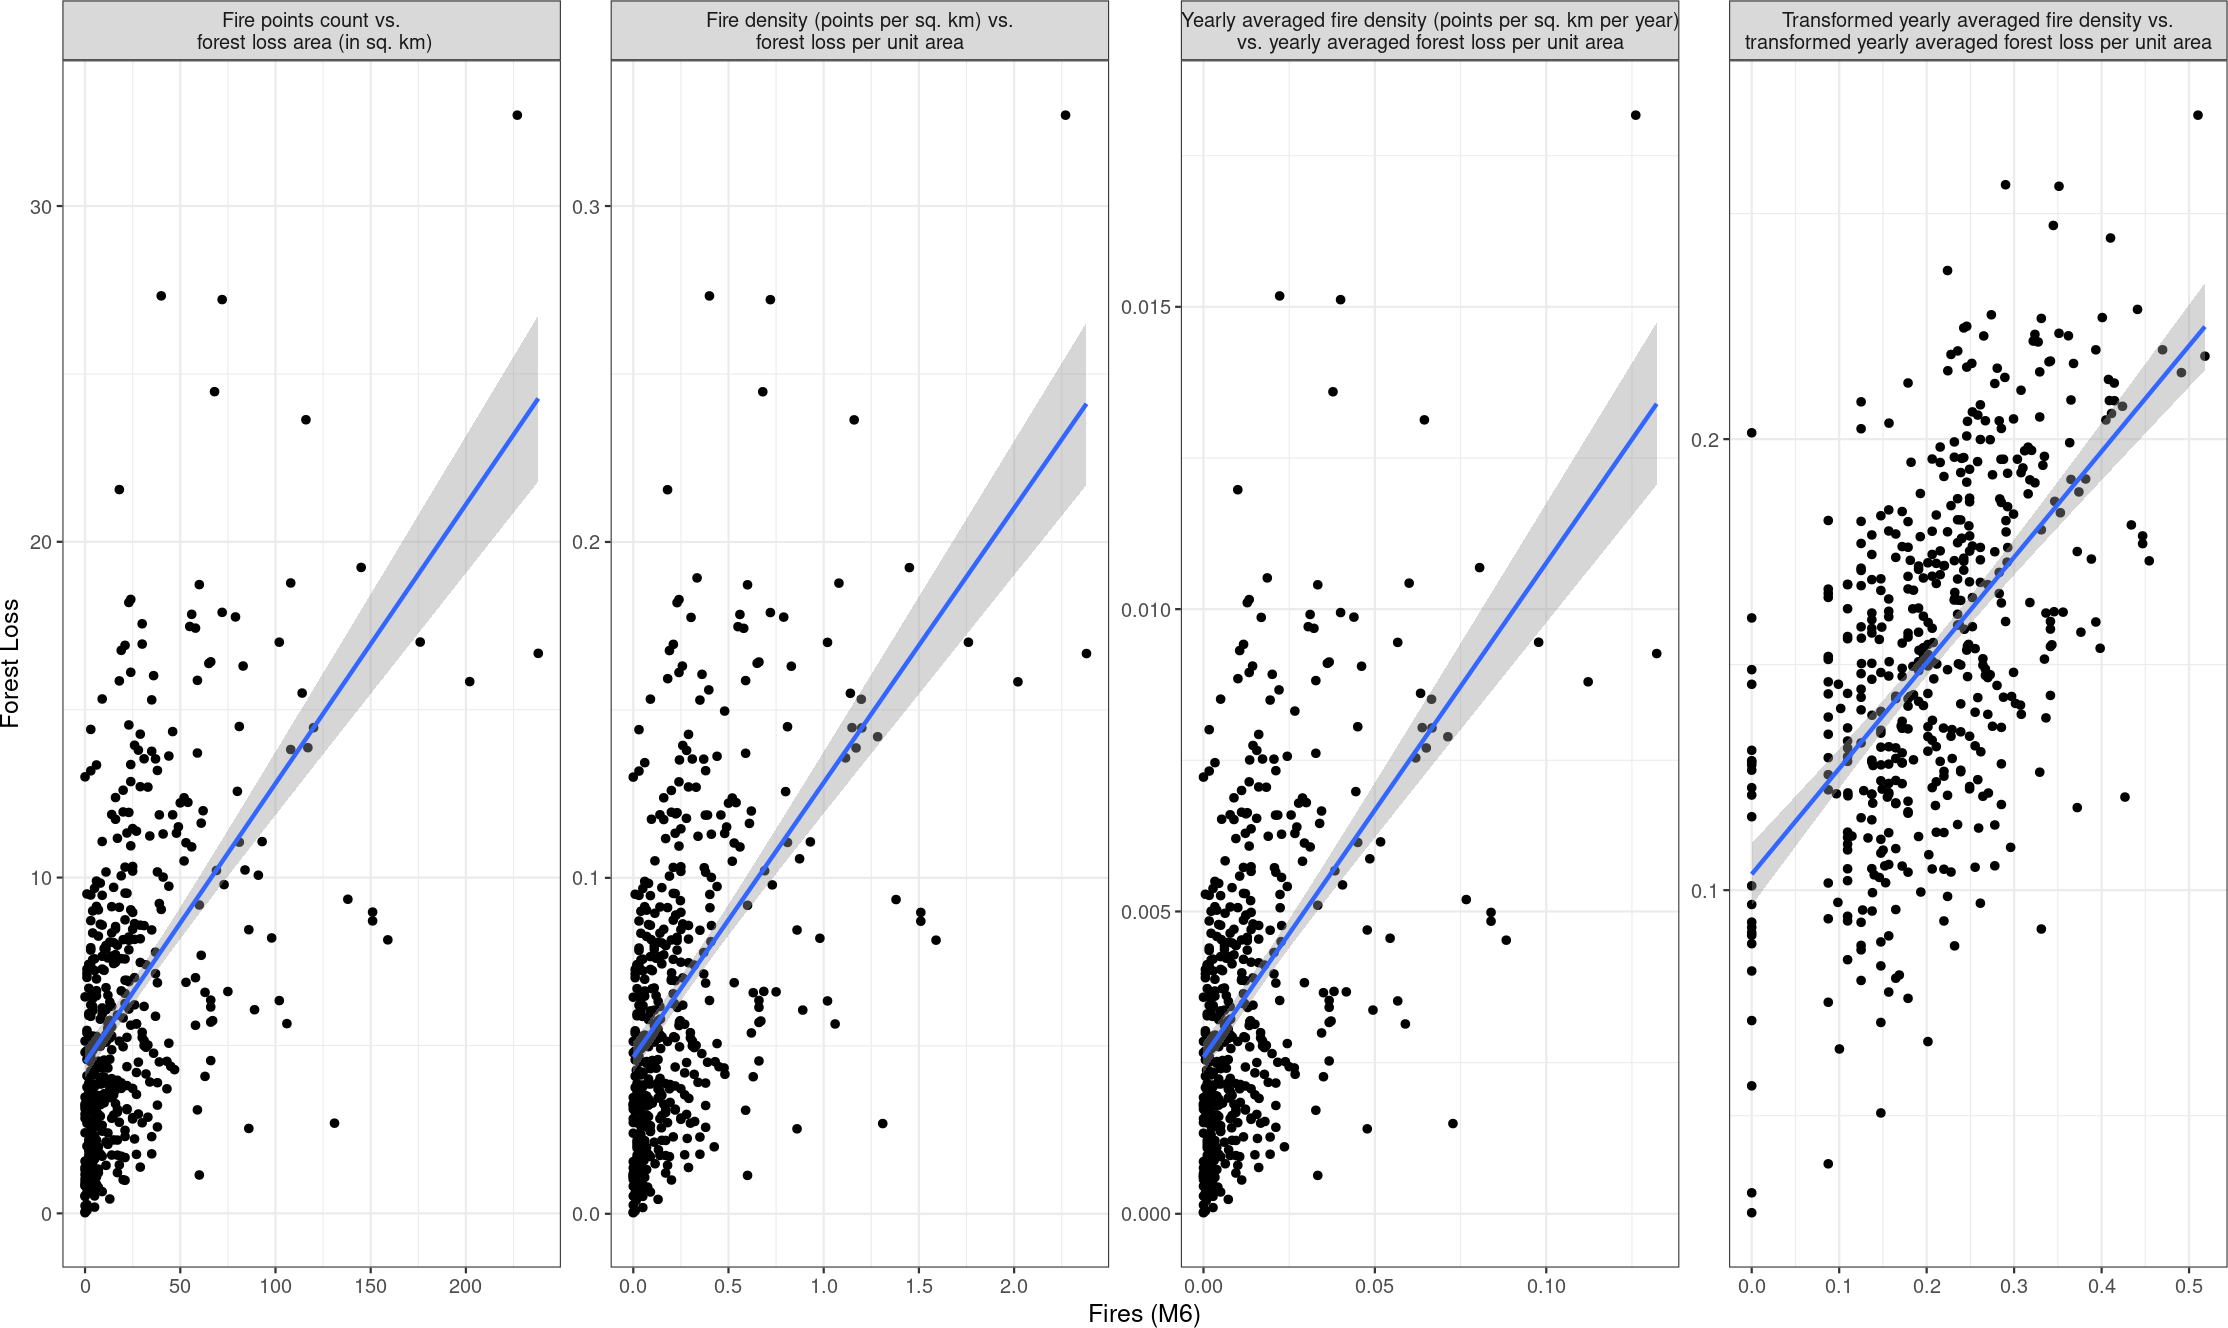
\includegraphics{img/modelling/lta-esda-14} \end{center}

\begin{Shaded}
\begin{Highlighting}[]
\CommentTok{\# QQ{-}norm}
\NormalTok{grdzonaledam6 }\SpecialCharTok{\%\textgreater{}\%}
\NormalTok{    st\_drop\_geometry }\SpecialCharTok{\%\textgreater{}\%}
\NormalTok{    dplyr}\SpecialCharTok{::}\FunctionTok{select}\NormalTok{(}\FunctionTok{matches}\NormalTok{(}\StringTok{".*PSQKM\_PYR$|.*PUA\_PYR$|.*PYR\_TLP$|.*PYR\_NORM$"}\NormalTok{)) }\SpecialCharTok{\%\textgreater{}\%}
    \FunctionTok{gather}\NormalTok{(key, val) }\SpecialCharTok{\%\textgreater{}\%}
    \FunctionTok{mutate}\NormalTok{(}\AttributeTok{key =}\NormalTok{ stringi}\SpecialCharTok{::}\FunctionTok{stri\_replace\_all\_regex}\NormalTok{(}\AttributeTok{str =}\NormalTok{ key, }\AttributeTok{pattern =} \FunctionTok{c}\NormalTok{(}\StringTok{".*PSQKM\_PYR$"}\NormalTok{,}
        \StringTok{".*PUA\_PYR$"}\NormalTok{, }\StringTok{".*PYR\_TLP$"}\NormalTok{, }\StringTok{".*PYR\_NORM$"}\NormalTok{), }\AttributeTok{replacement =} \FunctionTok{c}\NormalTok{(}\StringTok{"Yearly averaged fire density (points per sq. km per year)"}\NormalTok{,}
        \StringTok{"Yearly averaged forest loss per unit area"}\NormalTok{, }\StringTok{"Transformed yearly averaged fire density"}\NormalTok{,}
        \StringTok{"Transformed yearly averaged forest loss per unit area"}\NormalTok{), }\AttributeTok{vectorize\_all =}\NormalTok{ F)) }\SpecialCharTok{\%\textgreater{}\%}
    \FunctionTok{mutate}\NormalTok{(}\AttributeTok{key =} \FunctionTok{factor}\NormalTok{(key, }\AttributeTok{levels =} \FunctionTok{sort}\NormalTok{(}\FunctionTok{unique}\NormalTok{(key))[}\FunctionTok{c}\NormalTok{(}\DecValTok{3}\NormalTok{, }\DecValTok{4}\NormalTok{, }\DecValTok{1}\NormalTok{, }\DecValTok{2}\NormalTok{)])) }\SpecialCharTok{\%\textgreater{}\%}
\NormalTok{    ggplot }\SpecialCharTok{+} \FunctionTok{aes}\NormalTok{(}\AttributeTok{sample =}\NormalTok{ val) }\SpecialCharTok{+} \FunctionTok{geom\_qq}\NormalTok{() }\SpecialCharTok{+} \FunctionTok{facet\_wrap}\NormalTok{(}\SpecialCharTok{\textasciitilde{}}\NormalTok{key, }\AttributeTok{scales =} \StringTok{"free\_y"}\NormalTok{,}
    \AttributeTok{nrow =} \DecValTok{2}\NormalTok{, }\AttributeTok{dir =} \StringTok{"h"}\NormalTok{) }\SpecialCharTok{+} \FunctionTok{theme\_bw}\NormalTok{() }\SpecialCharTok{+} \FunctionTok{theme}\NormalTok{(}\AttributeTok{text =} \FunctionTok{element\_text}\NormalTok{(}\AttributeTok{size =} \DecValTok{14}\NormalTok{), }\AttributeTok{aspect.ratio =} \DecValTok{1}\NormalTok{)}
\end{Highlighting}
\end{Shaded}

\begin{center}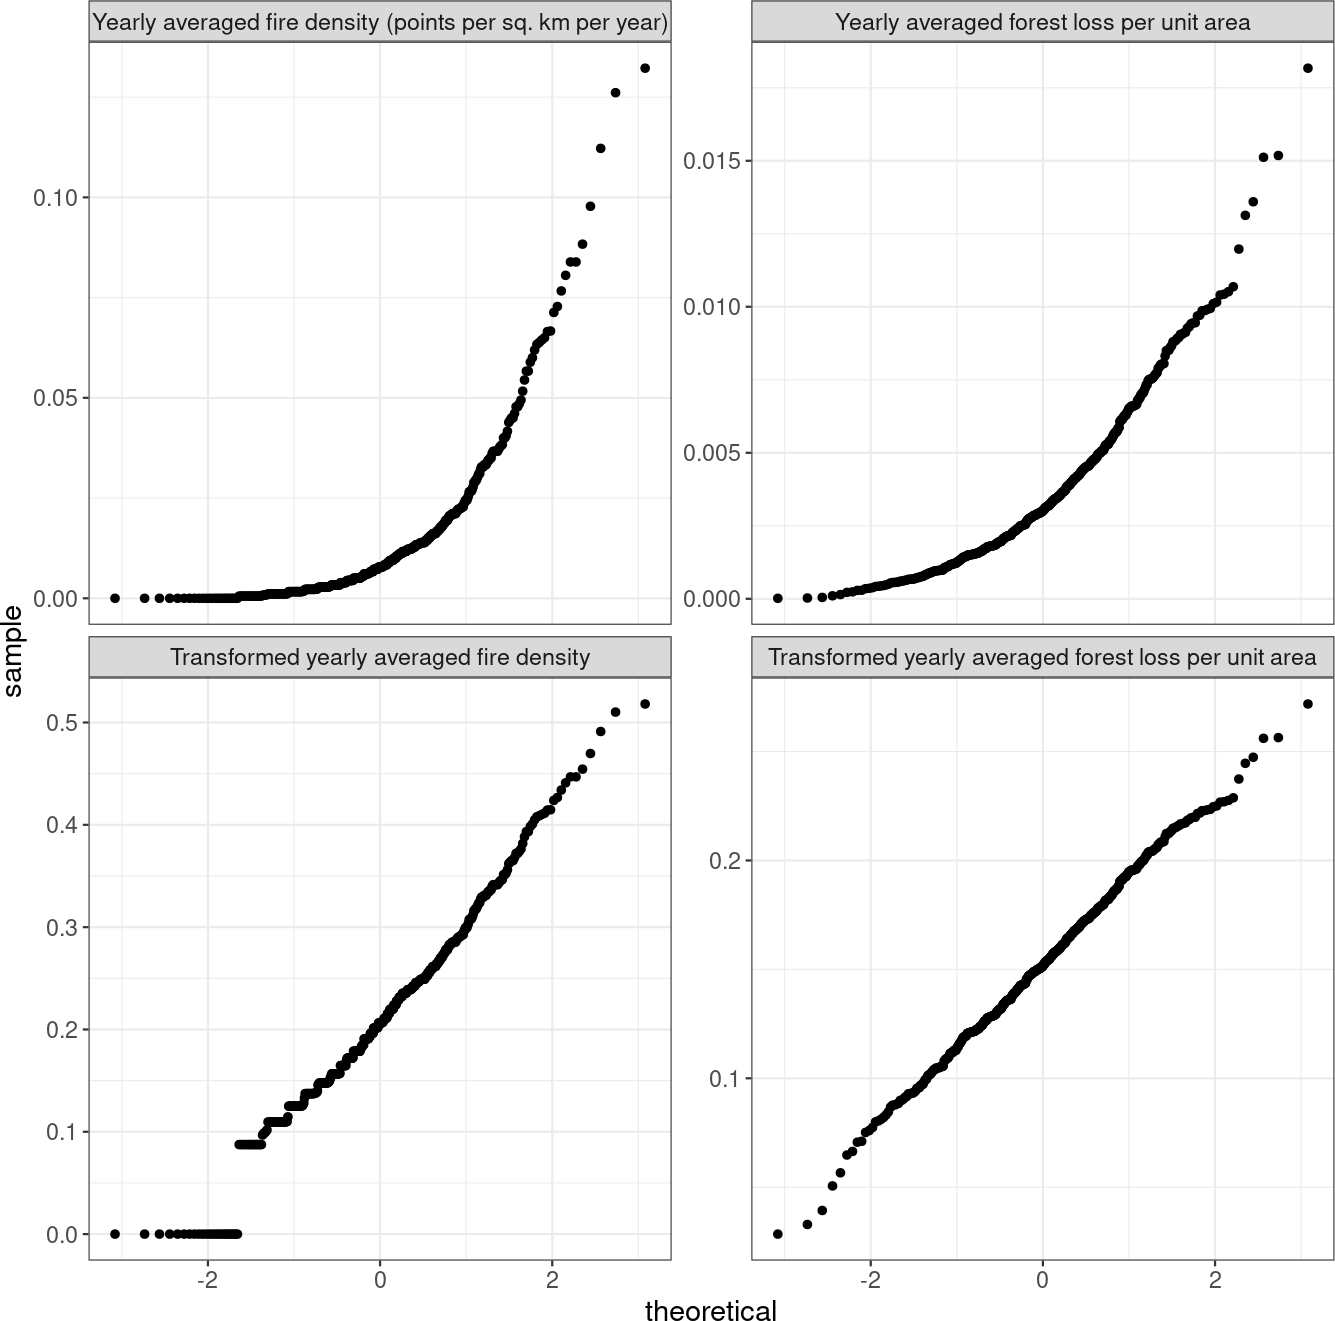
\includegraphics{img/modelling/lta-esda-15} \end{center}

\begin{Shaded}
\begin{Highlighting}[]
\CommentTok{\# Maps (for manuscript)}
\NormalTok{\{}
    \CommentTok{\# jpeg(\textquotesingle{}out/maps\_loss0118\_loss1218\_firesm6\_firesv1.jpg\textquotesingle{}, width = 3840,}
    \CommentTok{\# height = 2160, res = 250)}
\NormalTok{    grdzonal }\SpecialCharTok{\%\textgreater{}\%}
\NormalTok{        dplyr}\SpecialCharTok{::}\FunctionTok{select}\NormalTok{(}\StringTok{\textasciigrave{}}\AttributeTok{(A)}\StringTok{\textasciigrave{}} \OtherTok{=}\NormalTok{ LOSS0118\_PUA, }\StringTok{\textasciigrave{}}\AttributeTok{(B)}\StringTok{\textasciigrave{}} \OtherTok{=}\NormalTok{ LOSS1218\_PUA, }\StringTok{\textasciigrave{}}\AttributeTok{(C)}\StringTok{\textasciigrave{}} \OtherTok{=}\NormalTok{ NFIRESM6\_PSQKM,}
            \StringTok{\textasciigrave{}}\AttributeTok{(D)}\StringTok{\textasciigrave{}} \OtherTok{=}\NormalTok{ NFIRESV1\_PSQKM) }\SpecialCharTok{\%\textgreater{}\%}
        \FunctionTok{mutate\_if}\NormalTok{(is.numeric, }\FunctionTok{funs}\NormalTok{(. }\SpecialCharTok{*} \DecValTok{100}\NormalTok{)) }\SpecialCharTok{\%\textgreater{}\%}
        \FunctionTok{replace}\NormalTok{(}\FunctionTok{is.na}\NormalTok{(.), }\DecValTok{0}\NormalTok{) }\SpecialCharTok{\%\textgreater{}\%}
        \FunctionTok{gather}\NormalTok{(variable, value, }\SpecialCharTok{{-}}\NormalTok{geometry) }\SpecialCharTok{\%\textgreater{}\%}
        \FunctionTok{mutate}\NormalTok{(}\AttributeTok{variable =} \FunctionTok{factor}\NormalTok{(variable, }\AttributeTok{levels =} \FunctionTok{unique}\NormalTok{(variable))) }\SpecialCharTok{\%\textgreater{}\%}
        \FunctionTok{tm\_shape}\NormalTok{() }\SpecialCharTok{+} \FunctionTok{tm\_fill}\NormalTok{(}\AttributeTok{col =} \StringTok{"value"}\NormalTok{, }\AttributeTok{palette =} \FunctionTok{c}\NormalTok{(}\StringTok{"\#c9eebd"}\NormalTok{, }\StringTok{"\#69d6bd"}\NormalTok{, }\StringTok{"\#00bdc1"}\NormalTok{,}
        \StringTok{"\#10858d"}\NormalTok{), }\AttributeTok{size =} \FloatTok{0.1}\NormalTok{, }\AttributeTok{style =} \StringTok{"kmeans"}\NormalTok{, }\AttributeTok{legend.is.portrait =}\NormalTok{ T, }\AttributeTok{legend.format =} \FunctionTok{list}\NormalTok{(}\AttributeTok{digits =} \DecValTok{2}\NormalTok{,}
        \AttributeTok{text.separator =} \StringTok{"{-}"}\NormalTok{), }\AttributeTok{n =} \DecValTok{4}\NormalTok{) }\SpecialCharTok{+} \FunctionTok{tm\_borders}\NormalTok{(}\AttributeTok{col =} \StringTok{"grey15"}\NormalTok{, }\AttributeTok{lwd =} \FloatTok{0.3}\NormalTok{) }\SpecialCharTok{+} \FunctionTok{tm\_facets}\NormalTok{(}\AttributeTok{by =} \StringTok{"variable"}\NormalTok{,}
        \AttributeTok{nrow =} \DecValTok{2}\NormalTok{, }\AttributeTok{free.coords =} \ConstantTok{FALSE}\NormalTok{, }\AttributeTok{free.scales =} \ConstantTok{TRUE}\NormalTok{) }\SpecialCharTok{+} \FunctionTok{tm\_layout}\NormalTok{(}\AttributeTok{panel.label.size =} \DecValTok{3}\NormalTok{,}
        \AttributeTok{legend.title.size =} \FloatTok{1e{-}04}\NormalTok{, }\AttributeTok{legend.text.size =} \FloatTok{1.8}\NormalTok{, }\AttributeTok{bg.color =} \StringTok{"grey90"}\NormalTok{, }\AttributeTok{legend.format =} \FunctionTok{list}\NormalTok{(}\AttributeTok{scientific =} \ConstantTok{TRUE}\NormalTok{,}
            \AttributeTok{fun =} \ControlFlowTok{function}\NormalTok{(x) }\FunctionTok{formatC}\NormalTok{(x, }\AttributeTok{digits =} \DecValTok{2}\NormalTok{, }\AttributeTok{format =} \StringTok{"f"}\NormalTok{))) }\SpecialCharTok{+} \FunctionTok{tm\_shape}\NormalTok{(seaocean) }\SpecialCharTok{+}
        \FunctionTok{tm\_borders}\NormalTok{() }\SpecialCharTok{+} \FunctionTok{tm\_fill}\NormalTok{(}\AttributeTok{col =} \StringTok{"white"}\NormalTok{) }\SpecialCharTok{+} \FunctionTok{tm\_shape}\NormalTok{(points\_of\_interest) }\SpecialCharTok{+} \FunctionTok{tm\_text}\NormalTok{(}\StringTok{"code"}\NormalTok{,}
        \AttributeTok{size =} \DecValTok{2}\NormalTok{, }\AttributeTok{col =} \StringTok{"black"}\NormalTok{, }\AttributeTok{fontface =} \StringTok{"bold"}\NormalTok{, }\AttributeTok{bg.color =} \StringTok{"white"}\NormalTok{, }\AttributeTok{bg.alpha =} \FloatTok{0.5}\NormalTok{)}
    \CommentTok{\# dev.off()}
\NormalTok{\}}
\end{Highlighting}
\end{Shaded}

\begin{center}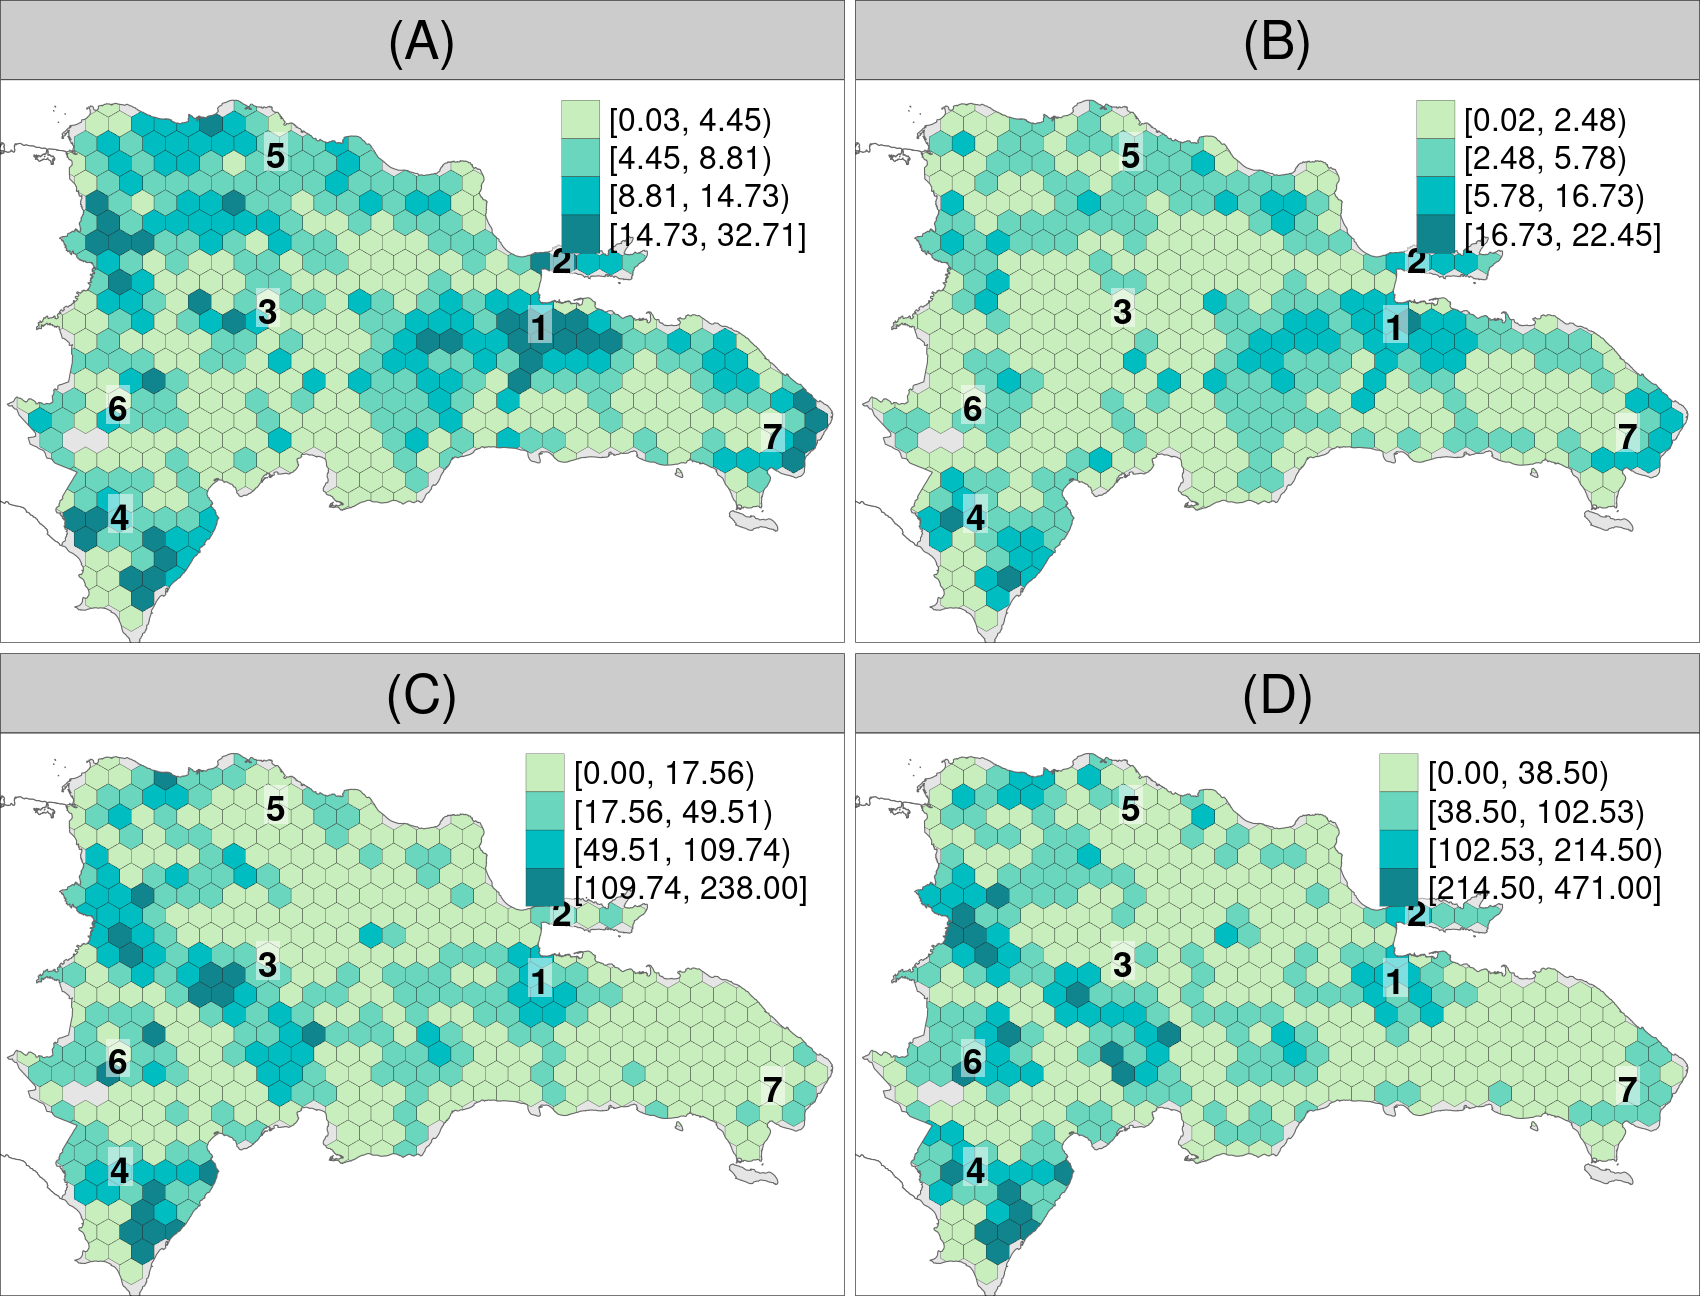
\includegraphics{img/modelling/lta-esda-16} \end{center}

\hypertarget{spatial-autoregressive-model-2001-2018}{%
\subsection{Spatial autoregressive model:
2001-2018}\label{spatial-autoregressive-model-2001-2018}}

\begin{Shaded}
\begin{Highlighting}[]
\CommentTok{\# ** LM LOSS0118\_PUA\_PYR\_NORM \textasciitilde{} NFIRESM6\_PSQKM\_PYR\_TLP}
\NormalTok{grdzonal }\SpecialCharTok{\%\textgreater{}\%}
    \FunctionTok{st\_drop\_geometry}\NormalTok{() }\SpecialCharTok{\%\textgreater{}\%}
    \FunctionTok{replace}\NormalTok{(}\FunctionTok{is.na}\NormalTok{(.), }\DecValTok{0}\NormalTok{) }\SpecialCharTok{\%\textgreater{}\%}
\NormalTok{    remove\_rownames }\SpecialCharTok{\%\textgreater{}\%}
    \FunctionTok{column\_to\_rownames}\NormalTok{(}\StringTok{"ENLACE"}\NormalTok{) }\SpecialCharTok{\%\textgreater{}\%}
    \FunctionTok{lm}\NormalTok{(LOSS0118\_PUA\_PYR\_NORM }\SpecialCharTok{\textasciitilde{}}\NormalTok{ NFIRESM6\_PSQKM\_PYR\_TLP, }\AttributeTok{data =}\NormalTok{ .) }\OtherTok{{-}\textgreater{}}\NormalTok{ grdlm4}
\NormalTok{grdlm4 }\SpecialCharTok{\%\textgreater{}\%}
    \FunctionTok{summary}\NormalTok{()}
\DocumentationTok{\#\# }
\DocumentationTok{\#\# Call:}
\DocumentationTok{\#\# lm(formula = LOSS0118\_PUA\_PYR\_NORM \textasciitilde{} NFIRESM6\_PSQKM\_PYR\_TLP, }
\DocumentationTok{\#\#     data = .)}
\DocumentationTok{\#\# }
\DocumentationTok{\#\# Residuals:}
\DocumentationTok{\#\#       Min        1Q    Median        3Q       Max }
\DocumentationTok{\#\# {-}0.089725 {-}0.022791  0.001563  0.022809  0.097884 }
\DocumentationTok{\#\# }
\DocumentationTok{\#\# Coefficients:}
\DocumentationTok{\#\#                        Estimate Std. Error t value Pr(\textgreater{}|t|)    }
\DocumentationTok{\#\# (Intercept)            0.103522   0.003509   29.50   \textless{}2e{-}16 ***}
\DocumentationTok{\#\# NFIRESM6\_PSQKM\_PYR\_TLP 0.234352   0.015184   15.43   \textless{}2e{-}16 ***}
\DocumentationTok{\#\# {-}{-}{-}}
\DocumentationTok{\#\# Signif. codes:  0 \textquotesingle{}***\textquotesingle{} 0.001 \textquotesingle{}**\textquotesingle{} 0.01 \textquotesingle{}*\textquotesingle{} 0.05 \textquotesingle{}.\textquotesingle{} 0.1 \textquotesingle{} \textquotesingle{} 1}
\DocumentationTok{\#\# }
\DocumentationTok{\#\# Residual standard error: 0.03212 on 480 degrees of freedom}
\DocumentationTok{\#\# Multiple R{-}squared:  0.3317, Adjusted R{-}squared:  0.3303 }
\DocumentationTok{\#\# F{-}statistic: 238.2 on 1 and 480 DF,  p{-}value: \textless{} 2.2e{-}16}
\NormalTok{grdlm4 }\SpecialCharTok{\%\textgreater{}\%}
    \FunctionTok{AIC}\NormalTok{()}
\DocumentationTok{\#\# [1] {-}1942.651}
\NormalTok{grdlm4 }\SpecialCharTok{\%\textgreater{}\%}
    \FunctionTok{logLik}\NormalTok{()}
\DocumentationTok{\#\# \textquotesingle{}log Lik.\textquotesingle{} 974.3256 (df=3)}
\NormalTok{grdlm4 }\SpecialCharTok{\%\textgreater{}\%}
\NormalTok{    lmtest}\SpecialCharTok{::}\FunctionTok{bptest}\NormalTok{()  }\CommentTok{\#Heteroscedastic model }
\DocumentationTok{\#\# }
\DocumentationTok{\#\#  studentized Breusch{-}Pagan test}
\DocumentationTok{\#\# }
\DocumentationTok{\#\# data:  .}
\DocumentationTok{\#\# BP = 0.091206, df = 1, p{-}value = 0.7626}
\FunctionTok{lm.morantest}\NormalTok{(grdlm4, grdww)}
\DocumentationTok{\#\# }
\DocumentationTok{\#\#  Global Moran I for regression residuals}
\DocumentationTok{\#\# }
\DocumentationTok{\#\# data:  }
\DocumentationTok{\#\# model: lm(formula = LOSS0118\_PUA\_PYR\_NORM \textasciitilde{} NFIRESM6\_PSQKM\_PYR\_TLP,}
\DocumentationTok{\#\# data = .)}
\DocumentationTok{\#\# weights: grdww}
\DocumentationTok{\#\# }
\DocumentationTok{\#\# Moran I statistic standard deviate = 18.413, p{-}value \textless{} 2.2e{-}16}
\DocumentationTok{\#\# alternative hypothesis: greater}
\DocumentationTok{\#\# sample estimates:}
\DocumentationTok{\#\# Observed Moran I      Expectation         Variance }
\DocumentationTok{\#\#     0.5151532429    {-}0.0031706302     0.0007924433}
\CommentTok{\# Note to self: spatially autocorrelated residuals. This model is not suitable}
\CommentTok{\# to predict loss 01{-}18}

\CommentTok{\# Lagrange multiplier test}
\NormalTok{lmultests }\OtherTok{\textless{}{-}} \FunctionTok{lm.LMtests}\NormalTok{(}\AttributeTok{model =}\NormalTok{ grdlm4, }\AttributeTok{listw =}\NormalTok{ grdww, }\AttributeTok{test =} \FunctionTok{c}\NormalTok{(}\StringTok{"LMerr"}\NormalTok{, }\StringTok{"LMlag"}\NormalTok{,}
    \StringTok{"RLMerr"}\NormalTok{, }\StringTok{"RLMlag"}\NormalTok{))}
\NormalTok{lmultests}
\DocumentationTok{\#\# }
\DocumentationTok{\#\#  Lagrange multiplier diagnostics for spatial dependence}
\DocumentationTok{\#\# }
\DocumentationTok{\#\# data:  }
\DocumentationTok{\#\# model: lm(formula = LOSS0118\_PUA\_PYR\_NORM \textasciitilde{} NFIRESM6\_PSQKM\_PYR\_TLP,}
\DocumentationTok{\#\# data = .)}
\DocumentationTok{\#\# weights: grdww}
\DocumentationTok{\#\# }
\DocumentationTok{\#\# LMerr = 330, df = 1, p{-}value \textless{} 2.2e{-}16}
\DocumentationTok{\#\# }
\DocumentationTok{\#\# }
\DocumentationTok{\#\#  Lagrange multiplier diagnostics for spatial dependence}
\DocumentationTok{\#\# }
\DocumentationTok{\#\# data:  }
\DocumentationTok{\#\# model: lm(formula = LOSS0118\_PUA\_PYR\_NORM \textasciitilde{} NFIRESM6\_PSQKM\_PYR\_TLP,}
\DocumentationTok{\#\# data = .)}
\DocumentationTok{\#\# weights: grdww}
\DocumentationTok{\#\# }
\DocumentationTok{\#\# LMlag = 227.22, df = 1, p{-}value \textless{} 2.2e{-}16}
\DocumentationTok{\#\# }
\DocumentationTok{\#\# }
\DocumentationTok{\#\#  Lagrange multiplier diagnostics for spatial dependence}
\DocumentationTok{\#\# }
\DocumentationTok{\#\# data:  }
\DocumentationTok{\#\# model: lm(formula = LOSS0118\_PUA\_PYR\_NORM \textasciitilde{} NFIRESM6\_PSQKM\_PYR\_TLP,}
\DocumentationTok{\#\# data = .)}
\DocumentationTok{\#\# weights: grdww}
\DocumentationTok{\#\# }
\DocumentationTok{\#\# RLMerr = 106.49, df = 1, p{-}value \textless{} 2.2e{-}16}
\DocumentationTok{\#\# }
\DocumentationTok{\#\# }
\DocumentationTok{\#\#  Lagrange multiplier diagnostics for spatial dependence}
\DocumentationTok{\#\# }
\DocumentationTok{\#\# data:  }
\DocumentationTok{\#\# model: lm(formula = LOSS0118\_PUA\_PYR\_NORM \textasciitilde{} NFIRESM6\_PSQKM\_PYR\_TLP,}
\DocumentationTok{\#\# data = .)}
\DocumentationTok{\#\# weights: grdww}
\DocumentationTok{\#\# }
\DocumentationTok{\#\# RLMlag = 3.7185, df = 1, p{-}value = 0.05381}
\NormalTok{tlmultests }\OtherTok{\textless{}{-}} \FunctionTok{t}\NormalTok{(}\FunctionTok{sapply}\NormalTok{(lmultests, }\ControlFlowTok{function}\NormalTok{(x) }\FunctionTok{c}\NormalTok{(x}\SpecialCharTok{$}\NormalTok{statistic, x}\SpecialCharTok{$}\NormalTok{p.value)))}
\FunctionTok{colnames}\NormalTok{(tlmultests) }\OtherTok{\textless{}{-}} \FunctionTok{c}\NormalTok{(}\StringTok{"Statistic"}\NormalTok{, }\StringTok{"p{-}value"}\NormalTok{)}
\FunctionTok{printCoefmat}\NormalTok{(tlmultests) }\SpecialCharTok{\%\textgreater{}\%}
\NormalTok{    knitr}\SpecialCharTok{::}\FunctionTok{kable}\NormalTok{(}\AttributeTok{format =} \StringTok{"latex"}\NormalTok{, }\AttributeTok{digits =} \DecValTok{2}\NormalTok{)  }\CommentTok{\#Latex output for manuscript}
\DocumentationTok{\#\#        Statistic p{-}value}
\DocumentationTok{\#\# LMerr   329.9950  0.0000}
\DocumentationTok{\#\# LMlag   227.2204  0.0000}
\DocumentationTok{\#\# RLMerr  106.4931  0.0000}
\DocumentationTok{\#\# RLMlag    3.7185  0.0538}
\end{Highlighting}
\end{Shaded}

\begin{tabular}{l|r|r}
\hline
  & Statistic & p-value\\
\hline
LMerr & 330.00 & 0.00\\
\hline
LMlag & 227.22 & 0.00\\
\hline
RLMerr & 106.49 & 0.00\\
\hline
RLMlag & 3.72 & 0.05\\
\hline
\end{tabular}

\begin{Shaded}
\begin{Highlighting}[]
\CommentTok{\# Both LMerr and LMlag are statistically significant, so it is assumed that}
\CommentTok{\# either the lagged variable (with a lagsarlm model) or the error dependence}
\CommentTok{\# (with a errorsarlm model) improve the result. However, the robust counterpart}
\CommentTok{\# of LMlag, RLMlag, is not significant, so the error dependence robust test}
\CommentTok{\# (RLMerr) suggests that errorsarlm model is the most likely alternative.}

\CommentTok{\# ** ERROR SAR, LOSS0118\_PUA\_PYR\_NORM \textasciitilde{} NFIRESM6\_PSQKM\_PYR\_TLP}
\NormalTok{grdzonal }\SpecialCharTok{\%\textgreater{}\%}
    \FunctionTok{st\_drop\_geometry}\NormalTok{() }\SpecialCharTok{\%\textgreater{}\%}
    \FunctionTok{replace}\NormalTok{(}\FunctionTok{is.na}\NormalTok{(.), }\DecValTok{0}\NormalTok{) }\SpecialCharTok{\%\textgreater{}\%}
\NormalTok{    spatialreg}\SpecialCharTok{::}\FunctionTok{errorsarlm}\NormalTok{(LOSS0118\_PUA\_PYR\_NORM }\SpecialCharTok{\textasciitilde{}}\NormalTok{ NFIRESM6\_PSQKM\_PYR\_TLP, }\AttributeTok{data =}\NormalTok{ .,}
        \AttributeTok{listw =}\NormalTok{ grdww) }\OtherTok{{-}\textgreater{}}\NormalTok{ grdesar1}
\NormalTok{grdesar1 }\SpecialCharTok{\%\textgreater{}\%}
    \FunctionTok{summary}\NormalTok{(}\AttributeTok{Nagelkerke =}\NormalTok{ T)}
\DocumentationTok{\#\# }
\DocumentationTok{\#\# Call:}
\DocumentationTok{\#\# spatialreg::errorsarlm(formula = LOSS0118\_PUA\_PYR\_NORM \textasciitilde{} NFIRESM6\_PSQKM\_PYR\_TLP, }
\DocumentationTok{\#\#     data = ., listw = grdww)}
\DocumentationTok{\#\# }
\DocumentationTok{\#\# Residuals:}
\DocumentationTok{\#\#         Min          1Q      Median          3Q         Max }
\DocumentationTok{\#\# {-}0.08081042 {-}0.01558612  0.00064743  0.01430194  0.09576362 }
\DocumentationTok{\#\# }
\DocumentationTok{\#\# Type: error }
\DocumentationTok{\#\# Coefficients: (asymptotic standard errors) }
\DocumentationTok{\#\#                         Estimate Std. Error z value  Pr(\textgreater{}|z|)}
\DocumentationTok{\#\# (Intercept)            0.0986476  0.0050648  19.477 \textless{} 2.2e{-}16}
\DocumentationTok{\#\# NFIRESM6\_PSQKM\_PYR\_TLP 0.2497097  0.0154632  16.149 \textless{} 2.2e{-}16}
\DocumentationTok{\#\# }
\DocumentationTok{\#\# Lambda: 0.73146, LR test value: 243.26, p{-}value: \textless{} 2.22e{-}16}
\DocumentationTok{\#\# Asymptotic standard error: 0.036645}
\DocumentationTok{\#\#     z{-}value: 19.96, p{-}value: \textless{} 2.22e{-}16}
\DocumentationTok{\#\# Wald statistic: 398.42, p{-}value: \textless{} 2.22e{-}16}
\DocumentationTok{\#\# }
\DocumentationTok{\#\# Log likelihood: 1095.956 for error model}
\DocumentationTok{\#\# ML residual variance (sigma squared): 0.00053902, (sigma: 0.023217)}
\DocumentationTok{\#\# Nagelkerke pseudo{-}R{-}squared: 0.59654 }
\DocumentationTok{\#\# Number of observations: 482 }
\DocumentationTok{\#\# Number of parameters estimated: 4 }
\DocumentationTok{\#\# AIC: {-}2183.9, (AIC for lm: {-}1942.7)}
\NormalTok{spatialreg}\SpecialCharTok{::}\FunctionTok{bptest.Sarlm}\NormalTok{(grdesar1)}
\DocumentationTok{\#\# }
\DocumentationTok{\#\#  studentized Breusch{-}Pagan test}
\DocumentationTok{\#\# }
\DocumentationTok{\#\# data:  }
\DocumentationTok{\#\# BP = 0.45483, df = 1, p{-}value = 0.5001}
\NormalTok{grdesar1 }\SpecialCharTok{\%\textgreater{}\%}
    \FunctionTok{residuals.sarlm}\NormalTok{() }\SpecialCharTok{\%\textgreater{}\%}
    \FunctionTok{moran.test}\NormalTok{(}\AttributeTok{listw =}\NormalTok{ grdww)}
\DocumentationTok{\#\# }
\DocumentationTok{\#\#  Moran I test under randomisation}
\DocumentationTok{\#\# }
\DocumentationTok{\#\# data:  .  }
\DocumentationTok{\#\# weights: grdww    }
\DocumentationTok{\#\# }
\DocumentationTok{\#\# Moran I statistic standard deviate = {-}0.0012016, p{-}value = 0.5005}
\DocumentationTok{\#\# alternative hypothesis: greater}
\DocumentationTok{\#\# sample estimates:}
\DocumentationTok{\#\# Moran I statistic       Expectation          Variance }
\DocumentationTok{\#\#      {-}0.002112870      {-}0.002079002       0.000794349}

\CommentTok{\# Summaries}
\NormalTok{grdzonal}\SpecialCharTok{$}\NormalTok{NFIRESM6 }\SpecialCharTok{\%\textgreater{}\%}
    \FunctionTok{summary}\NormalTok{()}
\DocumentationTok{\#\#    Min. 1st Qu.  Median    Mean 3rd Qu.    Max.    NA\textquotesingle{}s }
\DocumentationTok{\#\#    1.00    5.25   14.00   25.47   30.75  238.00      24}
\NormalTok{grdzonal}\SpecialCharTok{$}\NormalTok{NFIRESM6\_PSQKM }\SpecialCharTok{\%\textgreater{}\%}
    \FunctionTok{summary}\NormalTok{()}
\DocumentationTok{\#\#    Min. 1st Qu.  Median    Mean 3rd Qu.    Max.    NA\textquotesingle{}s }
\DocumentationTok{\#\#  0.0100  0.0600  0.1500  0.2645  0.3200  2.3800      24}
\NormalTok{grdzonal}\SpecialCharTok{$}\NormalTok{NFIRESM6\_PSQKM\_PYR }\SpecialCharTok{\%\textgreater{}\%}
    \FunctionTok{summary}\NormalTok{()}
\DocumentationTok{\#\#     Min.  1st Qu.   Median     Mean  3rd Qu.     Max.     NA\textquotesingle{}s }
\DocumentationTok{\#\# 0.000556 0.003333 0.008333 0.014694 0.017778 0.132222       24}

\CommentTok{\# * Predict forest loss per unit area per year, based on number of fires per}
\CommentTok{\# 100 sq. km per year}
\NormalTok{rangenfm6\_100sqkm }\OtherTok{\textless{}{-}} \FunctionTok{seq}\NormalTok{(}\DecValTok{0}\NormalTok{, }\FunctionTok{max}\NormalTok{(grdzonal}\SpecialCharTok{$}\NormalTok{NFIRESM6\_PSQKM\_PYR, }\AttributeTok{na.rm =}\NormalTok{ T), }\AttributeTok{length.out =} \DecValTok{20}\NormalTok{) }\SpecialCharTok{*}
    \DecValTok{100}
\NormalTok{fl }\OtherTok{\textless{}{-}} \ConstantTok{NULL}
\NormalTok{nf }\OtherTok{\textless{}{-}} \ConstantTok{NULL}
\NormalTok{predictfor\_100 }\OtherTok{\textless{}{-}} \ConstantTok{NULL}
\ControlFlowTok{for}\NormalTok{ (nf }\ControlFlowTok{in} \DecValTok{1}\SpecialCharTok{:}\DecValTok{20}\NormalTok{) \{}
    \CommentTok{\# These are actual figures of number of fires}
\NormalTok{    fl }\OtherTok{\textless{}{-}}\NormalTok{ (}\FunctionTok{coef.sarlm}\NormalTok{(grdesar1)[[}\DecValTok{3}\NormalTok{]] }\SpecialCharTok{*}\NormalTok{ (rangenfm6\_100sqkm[nf]}\SpecialCharTok{\^{}}\FloatTok{0.325}\NormalTok{) }\SpecialCharTok{+} \FunctionTok{coef.sarlm}\NormalTok{(grdesar1)[[}\DecValTok{2}\NormalTok{]])}\SpecialCharTok{\^{}}\NormalTok{(}\DecValTok{1}\SpecialCharTok{/}\FloatTok{0.325}\NormalTok{)}
\NormalTok{    predictfor\_100[nf] }\OtherTok{\textless{}{-}}\NormalTok{ fl}
\NormalTok{\}}
\NormalTok{rangenfm6\_100sqkm}
\DocumentationTok{\#\#  [1]  0.0000000  0.6959064  1.3918129  2.0877193  2.7836257  3.4795322}
\DocumentationTok{\#\#  [7]  4.1754386  4.8713450  5.5672515  6.2631579  6.9590643  7.6549708}
\DocumentationTok{\#\# [13]  8.3508772  9.0467836  9.7426901 10.4385965 11.1345029 11.8304094}
\DocumentationTok{\#\# [19] 12.5263158 13.2222222}
\NormalTok{predictfor\_100}
\DocumentationTok{\#\#  [1] 0.0008033077 0.0301924015 0.0495802699 0.0672171021 0.0839111640}
\DocumentationTok{\#\#  [6] 0.0999852339 0.1156086838 0.1308840303 0.1458791457 0.1606418403}
\DocumentationTok{\#\# [11] 0.1752073637 0.1896026301 0.2038487673 0.2179627389 0.2319584219}
\DocumentationTok{\#\# [16] 0.2458473484 0.2596392313 0.2733423477 0.2869638222 0.3005098430}
\FunctionTok{diff}\NormalTok{((predictfor\_100 }\SpecialCharTok{*} \FloatTok{1e+06}\NormalTok{))}
\DocumentationTok{\#\#  [1] 29389.09 19387.87 17636.83 16694.06 16074.07 15623.45 15275.35 14995.12}
\DocumentationTok{\#\#  [9] 14762.69 14565.52 14395.27 14246.14 14113.97 13995.68 13888.93 13791.88}
\DocumentationTok{\#\# [17] 13703.12 13621.47 13546.02}
\FunctionTok{mean}\NormalTok{(}\FunctionTok{diff}\NormalTok{((predictfor\_100 }\SpecialCharTok{*} \FloatTok{1e+06}\NormalTok{)))}
\DocumentationTok{\#\# [1] 15774.03}
\end{Highlighting}
\end{Shaded}

\hypertarget{spatial-autoregressive-model-2012-2018}{%
\subsection{Spatial autoregressive model:
2012-2018}\label{spatial-autoregressive-model-2012-2018}}

\begin{Shaded}
\begin{Highlighting}[]
\CommentTok{\# ** ERROR SAR, LOSS1218\_PUA\_PYR\_NORM \textasciitilde{} NFIRESV1\_PSQKM\_PYR\_TLP}
\NormalTok{grdzonal }\SpecialCharTok{\%\textgreater{}\%}
    \FunctionTok{st\_drop\_geometry}\NormalTok{() }\SpecialCharTok{\%\textgreater{}\%}
    \FunctionTok{replace}\NormalTok{(}\FunctionTok{is.na}\NormalTok{(.), }\DecValTok{0}\NormalTok{) }\SpecialCharTok{\%\textgreater{}\%}
\NormalTok{    spatialreg}\SpecialCharTok{::}\FunctionTok{errorsarlm}\NormalTok{(LOSS1218\_PUA\_PYR\_NORM }\SpecialCharTok{\textasciitilde{}}\NormalTok{ NFIRESV1\_PSQKM\_PYR\_TLP, }\AttributeTok{data =}\NormalTok{ .,}
        \AttributeTok{listw =}\NormalTok{ grdww) }\OtherTok{{-}\textgreater{}}\NormalTok{ grdesarv1}
\NormalTok{grdesarv1 }\SpecialCharTok{\%\textgreater{}\%}
    \FunctionTok{summary}\NormalTok{(}\AttributeTok{Nagelkerke =}\NormalTok{ T)}
\DocumentationTok{\#\# }
\DocumentationTok{\#\# Call:}
\DocumentationTok{\#\# spatialreg::errorsarlm(formula = LOSS1218\_PUA\_PYR\_NORM \textasciitilde{} NFIRESV1\_PSQKM\_PYR\_TLP, }
\DocumentationTok{\#\#     data = ., listw = grdww)}
\DocumentationTok{\#\# }
\DocumentationTok{\#\# Residuals:}
\DocumentationTok{\#\#        Min         1Q     Median         3Q        Max }
\DocumentationTok{\#\# {-}0.1306098 {-}0.0207140  0.0020657  0.0194729  0.1263294 }
\DocumentationTok{\#\# }
\DocumentationTok{\#\# Type: error }
\DocumentationTok{\#\# Coefficients: (asymptotic standard errors) }
\DocumentationTok{\#\#                         Estimate Std. Error z value  Pr(\textgreater{}|z|)}
\DocumentationTok{\#\# (Intercept)            0.1729754  0.0079585  21.735 \textless{} 2.2e{-}16}
\DocumentationTok{\#\# NFIRESV1\_PSQKM\_PYR\_TLP 0.2468619  0.0138606  17.810 \textless{} 2.2e{-}16}
\DocumentationTok{\#\# }
\DocumentationTok{\#\# Lambda: 0.73987, LR test value: 252.43, p{-}value: \textless{} 2.22e{-}16}
\DocumentationTok{\#\# Asymptotic standard error: 0.035926}
\DocumentationTok{\#\#     z{-}value: 20.595, p{-}value: \textless{} 2.22e{-}16}
\DocumentationTok{\#\# Wald statistic: 424.14, p{-}value: \textless{} 2.22e{-}16}
\DocumentationTok{\#\# }
\DocumentationTok{\#\# Log likelihood: 936.7731 for error model}
\DocumentationTok{\#\# ML residual variance (sigma squared): 0.0010389, (sigma: 0.032232)}
\DocumentationTok{\#\# Nagelkerke pseudo{-}R{-}squared: 0.62438 }
\DocumentationTok{\#\# Number of observations: 482 }
\DocumentationTok{\#\# Number of parameters estimated: 4 }
\DocumentationTok{\#\# AIC: {-}1865.5, (AIC for lm: {-}1615.1)}
\NormalTok{spatialreg}\SpecialCharTok{::}\FunctionTok{bptest.Sarlm}\NormalTok{(grdesarv1)}
\DocumentationTok{\#\# }
\DocumentationTok{\#\#  studentized Breusch{-}Pagan test}
\DocumentationTok{\#\# }
\DocumentationTok{\#\# data:  }
\DocumentationTok{\#\# BP = 3.5829, df = 1, p{-}value = 0.05838}
\NormalTok{grdesarv1 }\SpecialCharTok{\%\textgreater{}\%}
    \FunctionTok{residuals.sarlm}\NormalTok{() }\SpecialCharTok{\%\textgreater{}\%}
    \FunctionTok{moran.test}\NormalTok{(}\AttributeTok{listw =}\NormalTok{ grdww)}
\DocumentationTok{\#\# }
\DocumentationTok{\#\#  Moran I test under randomisation}
\DocumentationTok{\#\# }
\DocumentationTok{\#\# data:  .  }
\DocumentationTok{\#\# weights: grdww    }
\DocumentationTok{\#\# }
\DocumentationTok{\#\# Moran I statistic standard deviate = {-}0.48027, p{-}value = 0.6845}
\DocumentationTok{\#\# alternative hypothesis: greater}
\DocumentationTok{\#\# sample estimates:}
\DocumentationTok{\#\# Moran I statistic       Expectation          Variance }
\DocumentationTok{\#\#     {-}0.0156087685     {-}0.0020790021      0.0007936127}

\CommentTok{\# * Predict forest loss per unit area per year, based on number of fires per}
\CommentTok{\# 100 sq. km per year}
\NormalTok{rangenfv1\_100sqkm }\OtherTok{\textless{}{-}} \FunctionTok{seq}\NormalTok{(}\DecValTok{0}\NormalTok{, }\FunctionTok{max}\NormalTok{(grdzonal}\SpecialCharTok{$}\NormalTok{NFIRESV1\_PSQKM\_PYR, }\AttributeTok{na.rm =}\NormalTok{ T), }\AttributeTok{length.out =} \DecValTok{20}\NormalTok{) }\SpecialCharTok{*}
    \DecValTok{100}
\NormalTok{fl }\OtherTok{\textless{}{-}} \ConstantTok{NULL}
\NormalTok{nf }\OtherTok{\textless{}{-}} \ConstantTok{NULL}
\NormalTok{predictfor1218\_100 }\OtherTok{\textless{}{-}} \ConstantTok{NULL}
\ControlFlowTok{for}\NormalTok{ (nf }\ControlFlowTok{in} \DecValTok{1}\SpecialCharTok{:}\DecValTok{20}\NormalTok{) \{}
    \CommentTok{\# These are actual figures of number of fires}
\NormalTok{    fl }\OtherTok{\textless{}{-}}\NormalTok{ (}\FunctionTok{coef.sarlm}\NormalTok{(grdesarv1)[[}\DecValTok{3}\NormalTok{]] }\SpecialCharTok{*}\NormalTok{ (rangenfv1\_100sqkm[nf]}\SpecialCharTok{\^{}}\FloatTok{0.3}\NormalTok{) }\SpecialCharTok{+} \FunctionTok{coef.sarlm}\NormalTok{(grdesarv1)[[}\DecValTok{2}\NormalTok{]])}\SpecialCharTok{\^{}}\NormalTok{(}\DecValTok{1}\SpecialCharTok{/}\FloatTok{0.225}\NormalTok{)}
\NormalTok{    predictfor1218\_100[nf] }\OtherTok{\textless{}{-}}\NormalTok{ fl}
\NormalTok{\}}
\NormalTok{rangenfv1\_100sqkm}
\DocumentationTok{\#\#  [1]  0.000000  3.541353  7.082707 10.624060 14.165414 17.706767 21.248120}
\DocumentationTok{\#\#  [8] 24.789474 28.330827 31.872180 35.413534 38.954887 42.496241 46.037594}
\DocumentationTok{\#\# [15] 49.578947 53.120301 56.661654 60.203008 63.744361 67.285714}
\NormalTok{predictfor1218\_100}
\DocumentationTok{\#\#  [1] 0.0004104529 0.0613867361 0.1170241017 0.1738126082 0.2318998617}
\DocumentationTok{\#\#  [6] 0.2912336711 0.3517354422 0.4133290569 0.4759463524 0.5395274084}
\DocumentationTok{\#\# [11] 0.6040196344 0.6693766847 0.7355574747 0.8025253515 0.8702474117}
\DocumentationTok{\#\# [16] 0.9386939454 1.0078379800 1.0776549064 1.1481221694 1.2192190098}
\FunctionTok{diff}\NormalTok{((predictfor1218\_100 }\SpecialCharTok{*} \FloatTok{1e+06}\NormalTok{))}
\DocumentationTok{\#\#  [1] 60976.28 55637.37 56788.51 58087.25 59333.81 60501.77 61593.61 62617.30}
\DocumentationTok{\#\#  [9] 63581.06 64492.23 65357.05 66180.79 66967.88 67722.06 68446.53 69144.03}
\DocumentationTok{\#\# [17] 69816.93 70467.26 71096.84}
\FunctionTok{mean}\NormalTok{(}\FunctionTok{diff}\NormalTok{((predictfor1218\_100 }\SpecialCharTok{*} \FloatTok{1e+06}\NormalTok{)))}
\DocumentationTok{\#\# [1] 64147.82}
\end{Highlighting}
\end{Shaded}

\hypertarget{model-prediction-comparison-2001-2018-and-2012-2018}{%
\subsection{Model prediction comparison: 2001-2018 and
2012-2018}\label{model-prediction-comparison-2001-2018-and-2012-2018}}

\begin{Shaded}
\begin{Highlighting}[]
\CommentTok{\# Plot}
\NormalTok{loss\_fire\_assoc\_df }\OtherTok{\textless{}{-}} \FunctionTok{data.frame}\NormalTok{(rangenfm6\_100sqkm, rangenfv1\_100sqkm, predictfor\_100,}
\NormalTok{    predictfor1218\_100)}
\NormalTok{loss\_fire\_assoc\_df }\SpecialCharTok{\%\textgreater{}\%}
    \FunctionTok{gather}\NormalTok{(variable, value) }\SpecialCharTok{\%\textgreater{}\%}
    \FunctionTok{mutate}\NormalTok{(}\AttributeTok{period =} \FunctionTok{ifelse}\NormalTok{(}\FunctionTok{grepl}\NormalTok{(}\StringTok{"v1|1218"}\NormalTok{, variable), }\StringTok{"2012{-}2018"}\NormalTok{, }\StringTok{"2001{-}2018"}\NormalTok{),}
        \AttributeTok{axis =} \FunctionTok{ifelse}\NormalTok{(}\FunctionTok{grepl}\NormalTok{(}\StringTok{"range"}\NormalTok{, variable), }\StringTok{"x"}\NormalTok{, }\StringTok{"y"}\NormalTok{), }\AttributeTok{id =} \DecValTok{1}\SpecialCharTok{:}\FunctionTok{nrow}\NormalTok{(.)) }\SpecialCharTok{\%\textgreater{}\%}
    \FunctionTok{select}\NormalTok{(period, axis, value) }\SpecialCharTok{\%\textgreater{}\%}
    \FunctionTok{group\_by}\NormalTok{(period, axis) }\SpecialCharTok{\%\textgreater{}\%}
    \FunctionTok{mutate}\NormalTok{(}\AttributeTok{rn =} \FunctionTok{row\_number}\NormalTok{()) }\SpecialCharTok{\%\textgreater{}\%}
    \FunctionTok{ungroup}\NormalTok{() }\SpecialCharTok{\%\textgreater{}\%}
    \FunctionTok{spread}\NormalTok{(axis, value) }\SpecialCharTok{\%\textgreater{}\%}
    \FunctionTok{ggplot}\NormalTok{() }\SpecialCharTok{+} \FunctionTok{aes}\NormalTok{(}\AttributeTok{x =}\NormalTok{ x, }\AttributeTok{y =}\NormalTok{ y, }\AttributeTok{colour =}\NormalTok{ period) }\SpecialCharTok{+} \FunctionTok{geom\_path}\NormalTok{()}
\end{Highlighting}
\end{Shaded}

\begin{center}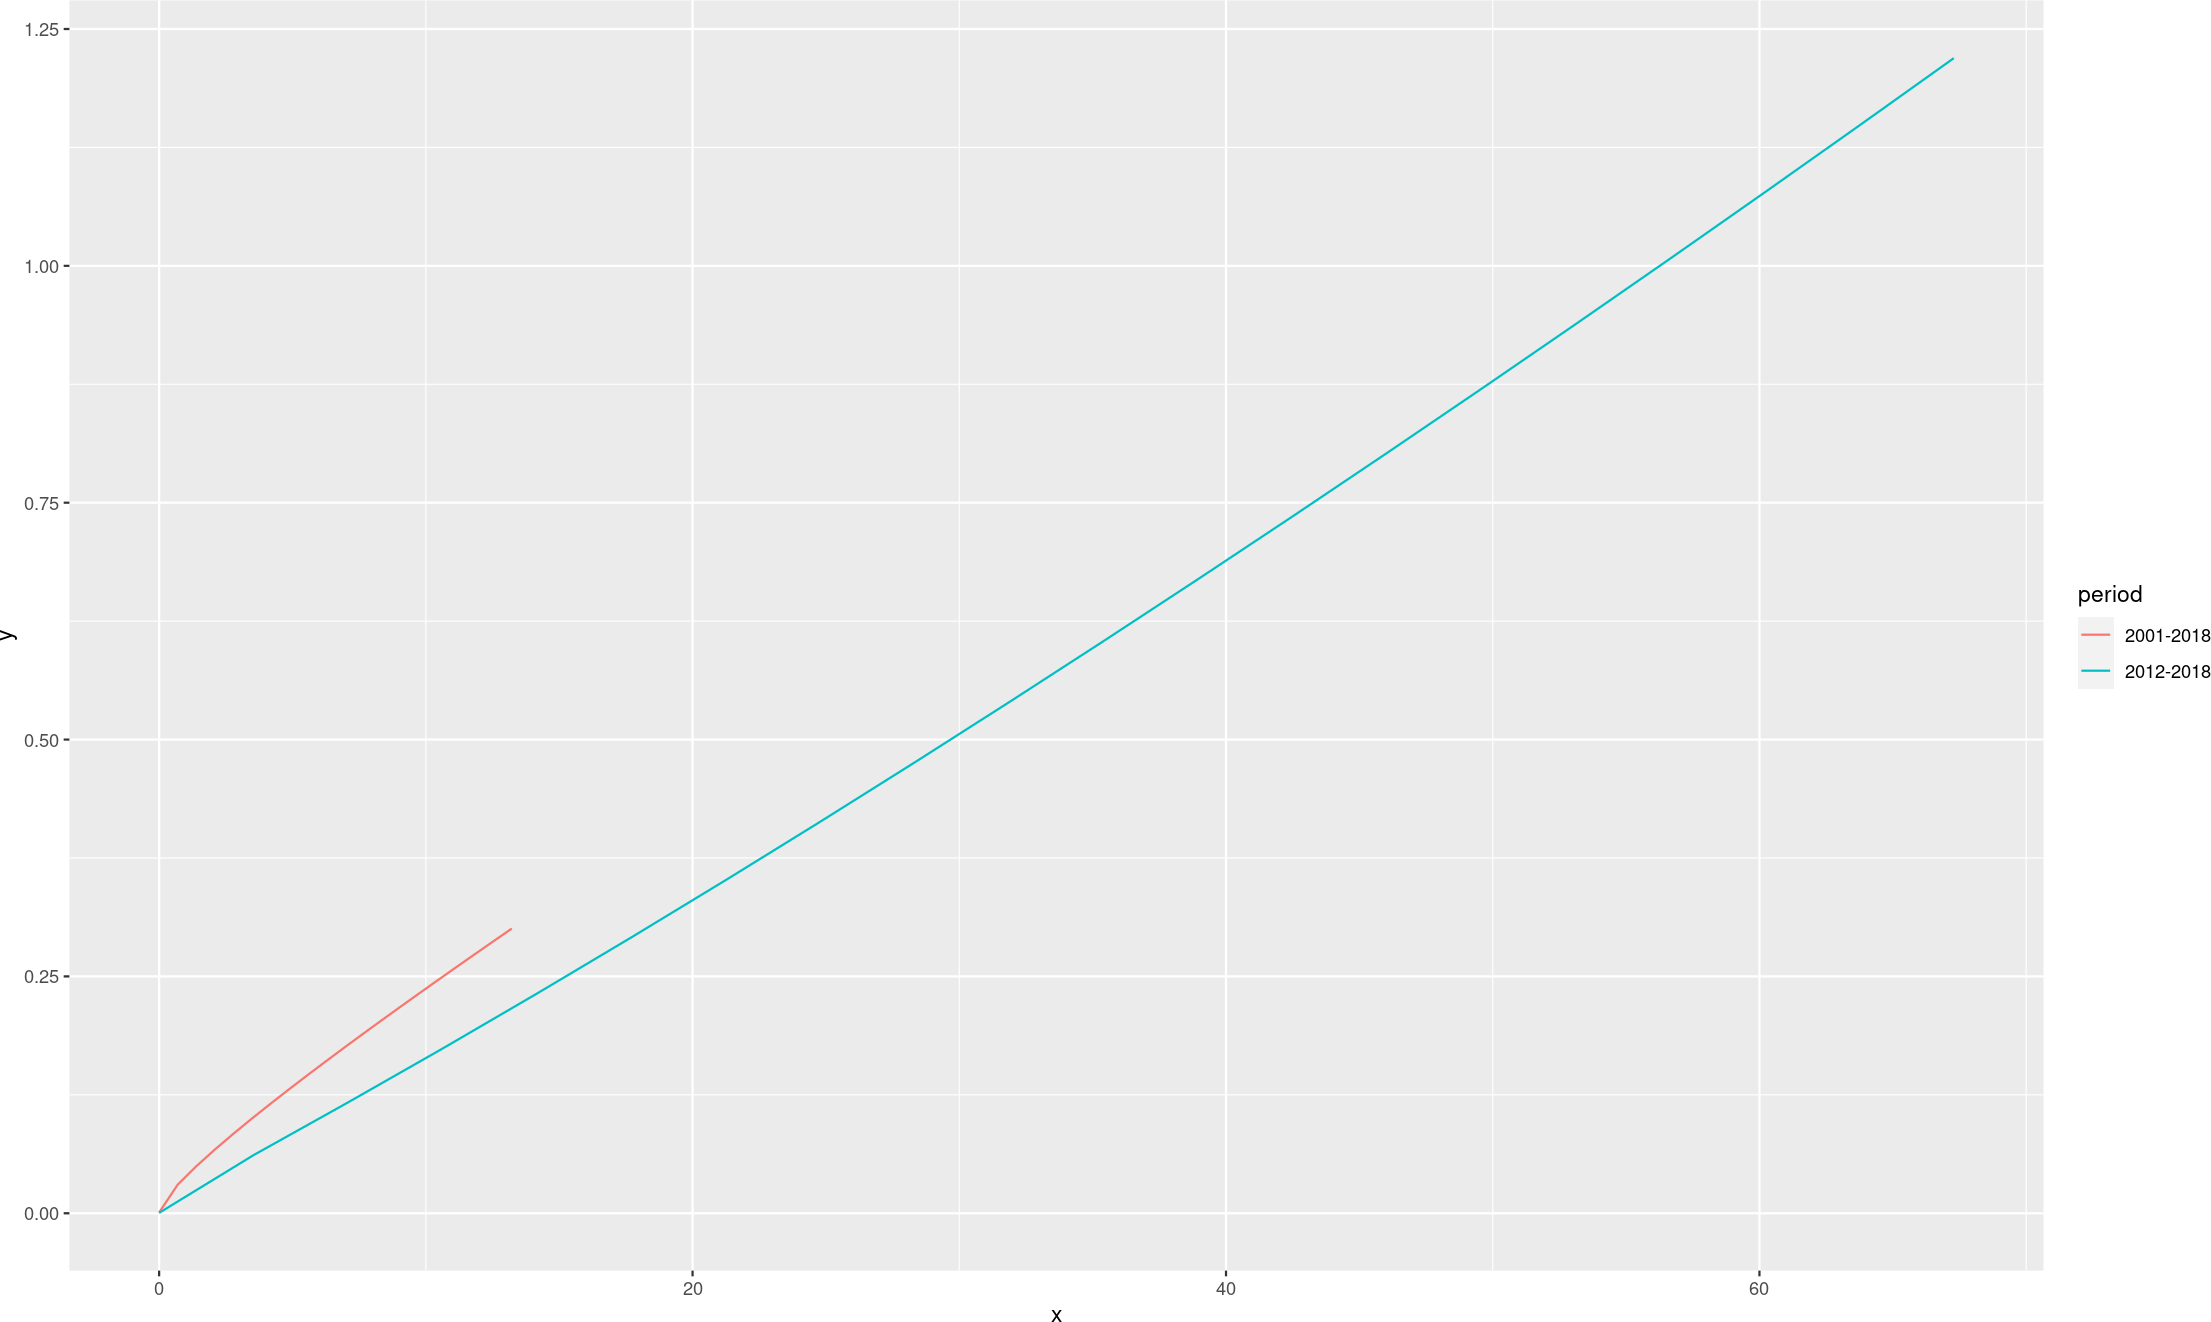
\includegraphics{img/modelling/lta-model-predictions-1} \end{center}

\hypertarget{modelling-for-the-annual-approach-using-forest-loss-as-dependent-variable-and-fires-m6-2001-2018-and-v1-2012-2018-as-independent-variables}{%
\section{\texorpdfstring{Modelling for the \textbf{annual approach},
using forest-loss as dependent variable, and fires M6 (2001-2018) and V1
(2012-2018) as independent
variables}{Modelling for the annual approach, using forest-loss as dependent variable, and fires M6 (2001-2018) and V1 (2012-2018) as independent variables}}\label{modelling-for-the-annual-approach-using-forest-loss-as-dependent-variable-and-fires-m6-2001-2018-and-v1-2012-2018-as-independent-variables}}

\hypertarget{neighbours}{%
\subsection{Neighbours}\label{neighbours}}

\begin{Shaded}
\begin{Highlighting}[]
\CommentTok{\#Zonal statistics object}
\NormalTok{hexzonal }\OtherTok{\textless{}{-}} \FunctionTok{readRDS}\NormalTok{(}\StringTok{\textquotesingle{}out/hex\_zonal\_statistics.RDS\textquotesingle{}}\NormalTok{)}
\NormalTok{hexzonalfm }\OtherTok{\textless{}{-}}\NormalTok{ hexzonal }\SpecialCharTok{\%\textgreater{}\%} \CommentTok{\# "fm" stands for "for modelling"}
\NormalTok{  dplyr}\SpecialCharTok{::}\FunctionTok{select}\NormalTok{(}\FunctionTok{matches}\NormalTok{(}\StringTok{\textquotesingle{}\^{}ENLACE$|\^{}AREASQM$|\^{}year([0{-}9])\{,2\}.loss1ha\_PCT$|NFIRES|NCLUMPSSMALLER1HA\textquotesingle{}}\NormalTok{)) }\SpecialCharTok{\%\textgreater{}\%} 
  \FunctionTok{mutate\_at}\NormalTok{(}\FunctionTok{vars}\NormalTok{(}\FunctionTok{matches}\NormalTok{(}\StringTok{\textquotesingle{}NFIRES|NCLUMPSSMALLER1HA\textquotesingle{}}\NormalTok{)), }\FunctionTok{funs}\NormalTok{(}\StringTok{"PSQKM"} \OtherTok{=}\NormalTok{ .}\SpecialCharTok{/}\NormalTok{(AREASQM}\SpecialCharTok{/}\DecValTok{1000000}\NormalTok{))) }\SpecialCharTok{\%\textgreater{}\%} 
  \FunctionTok{mutate\_at}\NormalTok{(}\FunctionTok{vars}\NormalTok{(}\FunctionTok{matches}\NormalTok{(}\StringTok{\textquotesingle{}PCT\textquotesingle{}}\NormalTok{)), }\FunctionTok{funs}\NormalTok{(}\StringTok{"PUA"} \OtherTok{=}\NormalTok{ .}\SpecialCharTok{/}\DecValTok{100}\NormalTok{)) }\SpecialCharTok{\%\textgreater{}\%} \CommentTok{\#Proportion per unit area}
  \FunctionTok{rename\_with}\NormalTok{(}\AttributeTok{.cols =} \FunctionTok{matches}\NormalTok{(}\StringTok{\textquotesingle{}PCT\_PUA\textquotesingle{}}\NormalTok{), }\AttributeTok{.fn =} \SpecialCharTok{\textasciitilde{}} \FunctionTok{gsub}\NormalTok{(}\StringTok{\textquotesingle{}PCT\_PUA\textquotesingle{}}\NormalTok{, }\StringTok{\textquotesingle{}PUA\textquotesingle{}}\NormalTok{, .)) }\SpecialCharTok{\%\textgreater{}\%} 
  \FunctionTok{rename\_with}\NormalTok{(}\AttributeTok{.cols =} \FunctionTok{matches}\NormalTok{(}\StringTok{\textquotesingle{}}\SpecialCharTok{\textbackslash{}\textbackslash{}}\StringTok{.\textquotesingle{}}\NormalTok{), }\AttributeTok{.fn =} \SpecialCharTok{\textasciitilde{}} \FunctionTok{gsub}\NormalTok{(}\StringTok{\textquotesingle{}}\SpecialCharTok{\textbackslash{}\textbackslash{}}\StringTok{.\textquotesingle{}}\NormalTok{, }\StringTok{\textquotesingle{}\_\textquotesingle{}}\NormalTok{, .)) }\SpecialCharTok{\%\textgreater{}\%} 
  \FunctionTok{rename\_with}\NormalTok{(}\AttributeTok{.fn =} \SpecialCharTok{\textasciitilde{}} \FunctionTok{gsub}\NormalTok{(}\StringTok{\textquotesingle{}loss1ha\textquotesingle{}}\NormalTok{, }\StringTok{\textquotesingle{}lossgreater1ha\textquotesingle{}}\NormalTok{, .)) }\SpecialCharTok{\%\textgreater{}\%} 
\NormalTok{  dplyr}\SpecialCharTok{::}\FunctionTok{select}\NormalTok{(}\FunctionTok{matches}\NormalTok{(}\StringTok{\textquotesingle{}\^{}ENLACE$|\^{}AREASQM$|PUA$|PSQKM$\textquotesingle{}}\NormalTok{)) }\SpecialCharTok{\%\textgreater{}\%} 
  \FunctionTok{rename\_at}\NormalTok{(}\FunctionTok{vars}\NormalTok{(}\SpecialCharTok{!}\FunctionTok{matches}\NormalTok{(}\StringTok{\textquotesingle{}\^{}geometry$\textquotesingle{}}\NormalTok{)), }\FunctionTok{funs}\NormalTok{(}\FunctionTok{toupper}\NormalTok{(.))) }\SpecialCharTok{\%\textgreater{}\%} 
  \FunctionTok{replace}\NormalTok{(}\FunctionTok{is.na}\NormalTok{(.), }\DecValTok{0}\NormalTok{)}

\CommentTok{\# * Neighbours, weight}
\NormalTok{hexnb }\OtherTok{\textless{}{-}} \FunctionTok{poly2nb}\NormalTok{(hexzonalfm)}
\FunctionTok{plot}\NormalTok{(}\FunctionTok{as\_Spatial}\NormalTok{(cline))}
\FunctionTok{plot}\NormalTok{(}\FunctionTok{as\_Spatial}\NormalTok{(hexzonalfm), }\AttributeTok{add=}\NormalTok{T)}
\FunctionTok{plot}\NormalTok{(hexnb, }\AttributeTok{coords =} \FunctionTok{coordinates}\NormalTok{(}\FunctionTok{as\_Spatial}\NormalTok{(hexzonalfm)), }\AttributeTok{add=}\NormalTok{T)}
\end{Highlighting}
\end{Shaded}

\begin{center}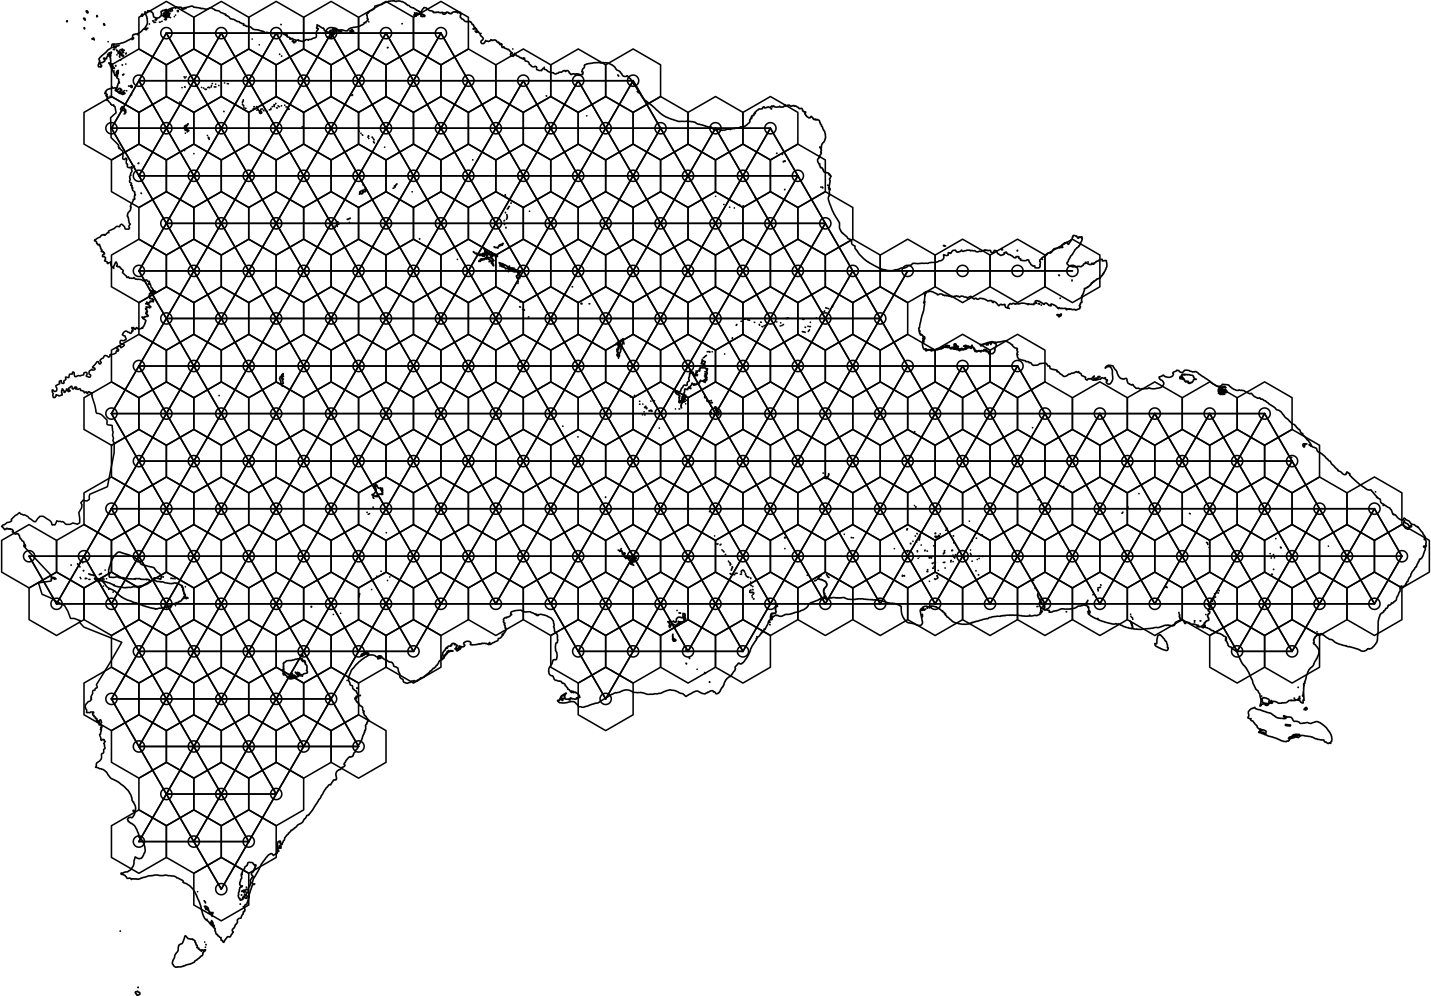
\includegraphics{img/modelling/aa-neighbours-1} \end{center}

\begin{Shaded}
\begin{Highlighting}[]
\FunctionTok{attr}\NormalTok{(hexnb, }\StringTok{\textquotesingle{}region.id\textquotesingle{}}\NormalTok{) }\OtherTok{\textless{}{-}}\NormalTok{ hexzonalfm}\SpecialCharTok{$}\NormalTok{ENLACE}
\NormalTok{hexww }\OtherTok{\textless{}{-}} \FunctionTok{nb2listw}\NormalTok{(hexnb, }\AttributeTok{zero.policy =}\NormalTok{ T)}
\NormalTok{hexww}
\DocumentationTok{\#\# Characteristics of weights list object:}
\DocumentationTok{\#\# Neighbour list object:}
\DocumentationTok{\#\# Number of regions: 253 }
\DocumentationTok{\#\# Number of nonzero links: 1342 }
\DocumentationTok{\#\# Percentage nonzero weights: 2.09658 }
\DocumentationTok{\#\# Average number of links: 5.304348 }
\DocumentationTok{\#\# }
\DocumentationTok{\#\# Weights style: W }
\DocumentationTok{\#\# Weights constants summary:}
\DocumentationTok{\#\#     n    nn  S0       S1       S2}
\DocumentationTok{\#\# W 253 64009 253 101.2822 1020.272}
\FunctionTok{plot}\NormalTok{(prov }\SpecialCharTok{\%\textgreater{}\%} \FunctionTok{st\_geometry}\NormalTok{(), }\AttributeTok{border =} \StringTok{\textquotesingle{}grey\textquotesingle{}}\NormalTok{)}
\FunctionTok{plot}\NormalTok{(hexzonalfm }\SpecialCharTok{\%\textgreater{}\%} \FunctionTok{st\_geometry}\NormalTok{(), }\AttributeTok{add=}\NormalTok{T, }\AttributeTok{border =} \StringTok{\textquotesingle{}red\textquotesingle{}}\NormalTok{)}
\FunctionTok{plot}\NormalTok{(hexnb, }\AttributeTok{coords =} \FunctionTok{coordinates}\NormalTok{(}\FunctionTok{as\_Spatial}\NormalTok{(hexzonalfm)), }\AttributeTok{add=}\NormalTok{T)}
\end{Highlighting}
\end{Shaded}

\begin{center}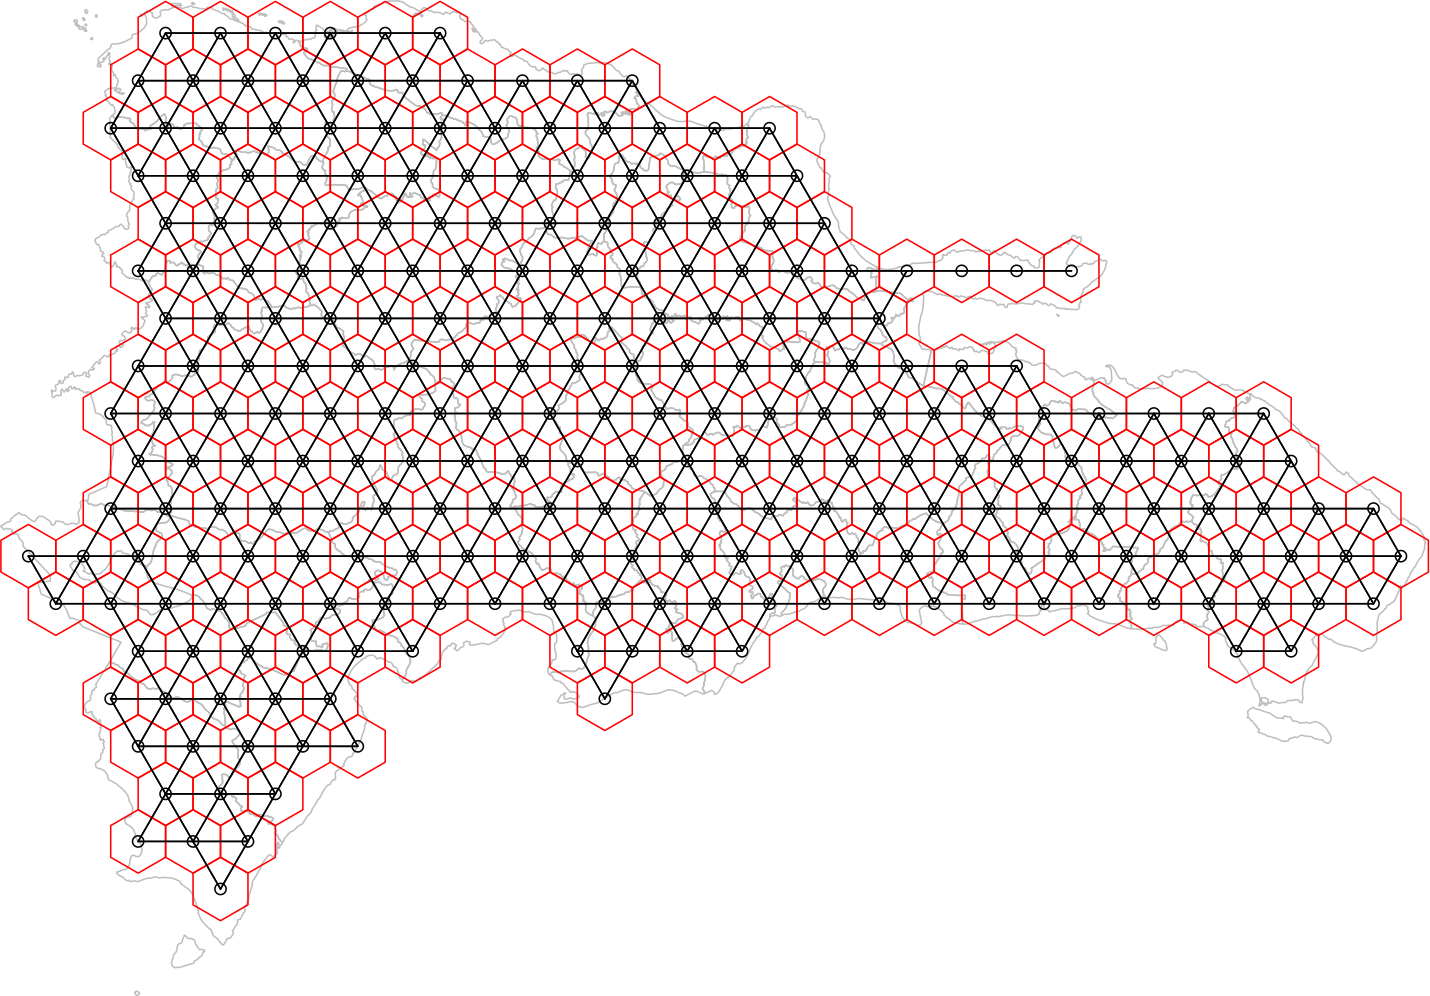
\includegraphics{img/modelling/aa-neighbours-2} \end{center}

\begin{Shaded}
\begin{Highlighting}[]
\NormalTok{hexwb }\OtherTok{\textless{}{-}} \FunctionTok{nb2listw}\NormalTok{(hexnb, }\AttributeTok{style =} \StringTok{\textquotesingle{}B\textquotesingle{}}\NormalTok{, }\AttributeTok{zero.policy =}\NormalTok{ T)}
\NormalTok{hexwb}
\DocumentationTok{\#\# Characteristics of weights list object:}
\DocumentationTok{\#\# Neighbour list object:}
\DocumentationTok{\#\# Number of regions: 253 }
\DocumentationTok{\#\# Number of nonzero links: 1342 }
\DocumentationTok{\#\# Percentage nonzero weights: 2.09658 }
\DocumentationTok{\#\# Average number of links: 5.304348 }
\DocumentationTok{\#\# }
\DocumentationTok{\#\# Weights style: B }
\DocumentationTok{\#\# Weights constants summary:}
\DocumentationTok{\#\#     n    nn   S0   S1    S2}
\DocumentationTok{\#\# B 253 64009 1342 2684 29808}
\end{Highlighting}
\end{Shaded}

\hypertarget{exploratory-data-analysis-eda-of-the-time-series}{%
\subsection{Exploratory data analysis (EDA) of the time
series}\label{exploratory-data-analysis-eda-of-the-time-series}}

\begin{Shaded}
\begin{Highlighting}[]
\CommentTok{\# ENTIRE DATASETS VALUES, SOURCES ARE VALUE RASTERS OF BOTH SMALL AND LARGE CLUMPS OF FOREST LOSS (SMALL CLEARINGS AND LARGE CLEARINGS). NO ZONAL DATA USED HERE}
\CommentTok{\# Forest loss from small clearings}
\CommentTok{\# losssmaller1ha\_byyear \textless{}{-} readRDS(\textquotesingle{}out/forest\_loss\_clumps\_smaller\_than\_1ha\_by\_year.RDS\textquotesingle{}) \# This file is big and when loaded as object "losssmaller1ha\_byyear" will take at least 20 GB of RAM. This is the reason why this line (and the subsequent ones) are commented. To ensure a smooth knitting, the object "foo" is created below using a readRDS function which loads the summary contained in the "summary\_of\_forest\_loss\_from\_small\_clearings.RDS" file.}
\CommentTok{\# foo \textless{}{-} sapply(names(losssmaller1ha\_byyear),}
\CommentTok{\#        function(x) \{}
\CommentTok{\#          length(which(!is.na(losssmaller1ha\_byyear[[x]][])))*prod(res(losssmaller1ha\_byyear[[x]]))}
\CommentTok{\#        \}}
\CommentTok{\# )}
\CommentTok{\# foo}
\CommentTok{\# saveRDS(foo, \textquotesingle{}out/summary\_of\_forest\_loss\_from\_small\_clearings.RDS\textquotesingle{})}
\CommentTok{\# rm(losssmaller1ha\_byyear)}
\CommentTok{\# gc()}
\NormalTok{(foo }\OtherTok{\textless{}{-}} \FunctionTok{readRDS}\NormalTok{(}\StringTok{\textquotesingle{}out/summary\_of\_forest\_loss\_from\_small\_clearings.RDS\textquotesingle{}}\NormalTok{))}
\DocumentationTok{\#\#     year1     year2     year3     year4     year5     year6     year7     year8 }
\DocumentationTok{\#\#  68097779  57987394  64155296  90843387  95712821  61348695  76193150  97650590 }
\DocumentationTok{\#\#     year9    year10    year11    year12    year13    year14    year15    year16 }
\DocumentationTok{\#\#  68417798  78545839  73057702 102396431  64542997  95576721  77698341 114961029 }
\DocumentationTok{\#\#    year17    year18 }
\DocumentationTok{\#\# 134721266  73972882}
\NormalTok{forest\_loss\_small\_clumps\_by\_year }\OtherTok{\textless{}{-}}\NormalTok{ foo }\SpecialCharTok{\%\textgreater{}\%} 
  \FunctionTok{enframe}\NormalTok{(}\AttributeTok{name =} \StringTok{\textquotesingle{}year\textquotesingle{}}\NormalTok{, }\AttributeTok{value =} \StringTok{\textquotesingle{}Small clearings (\textless{}1ha)\textquotesingle{}}\NormalTok{) }\SpecialCharTok{\%\textgreater{}\%} 
  \FunctionTok{mutate}\NormalTok{(}\AttributeTok{year =} \FunctionTok{as.numeric}\NormalTok{(}\FunctionTok{gsub}\NormalTok{(}\StringTok{\textquotesingle{}year\textquotesingle{}}\NormalTok{, }\StringTok{\textquotesingle{}\textquotesingle{}}\NormalTok{, year)) }\SpecialCharTok{+} \DecValTok{2000}\NormalTok{)}

\CommentTok{\# Forest loss from medium{-} and large clearings}
\CommentTok{\# loss1ha\_firesm6\_2500\_byyear \textless{}{-} readRDS(\textquotesingle{}out/forest\_loss\_1ha\_firesm6\_2500\_buffer\_by\_year.RDS\textquotesingle{}) \# This file is big and when loaded as object "loss1ha\_firesm6\_2500\_byyear" will take at least 20 GB of RAM. This is the reason why this line (and the subsequent ones) are commented. To ensure a smooth knitting, the object "foo" is created below using a readRDS function which loads the summary contained in the "summary\_of\_forest\_loss\_from\_medium\_large\_clearings.RDS" file.}
\CommentTok{\# loss1ha\_solo \textless{}{-} loss1ha\_firesm6\_2500\_byyear[grep(\textquotesingle{}loss1ha$\textquotesingle{}, names(loss1ha\_firesm6\_2500\_byyear))]}
\CommentTok{\# bar \textless{}{-} sapply(names(loss1ha\_solo),}
\CommentTok{\#        function(x) \{}
\CommentTok{\#          length(which(!is.na(loss1ha\_solo[[x]][])))*prod(res(loss1ha\_solo[[x]]))}
\CommentTok{\#        \}}
\CommentTok{\# )}
\CommentTok{\# names(bar) \textless{}{-} gsub(\textquotesingle{}(.*)(year[0{-}9]\{,2\})(.*)\textquotesingle{}, \textquotesingle{}\textbackslash{}\textbackslash{}2\textquotesingle{}, names(bar))}
\CommentTok{\# saveRDS(bar, \textquotesingle{}out/summary\_of\_forest\_loss\_from\_medium\_large\_clearings.RDS\textquotesingle{})}
\CommentTok{\# rm(loss1ha\_solo)}
\CommentTok{\# rm(loss1ha\_firesm6\_2500\_byyear)}
\CommentTok{\# gc()}
\NormalTok{(bar }\OtherTok{\textless{}{-}} \FunctionTok{readRDS}\NormalTok{(}\StringTok{\textquotesingle{}out/summary\_of\_forest\_loss\_from\_medium\_large\_clearings.RDS\textquotesingle{}}\NormalTok{))}
\DocumentationTok{\#\#     year1     year2     year3     year4     year5     year6     year7     year8 }
\DocumentationTok{\#\#  49320404  51640724  48640640 112483274 163901824  83138660  93631596 128039127 }
\DocumentationTok{\#\#     year9    year10    year11    year12    year13    year14    year15    year16 }
\DocumentationTok{\#\#  78809947  68351587  63621931  91351003 113665504  83709544 108977782 176083871 }
\DocumentationTok{\#\#    year17    year18 }
\DocumentationTok{\#\# 195739642 108533434}
\NormalTok{forest\_loss\_large\_clumps\_by\_year }\OtherTok{\textless{}{-}}\NormalTok{ bar }\SpecialCharTok{\%\textgreater{}\%} 
  \FunctionTok{enframe}\NormalTok{(}\AttributeTok{name =} \StringTok{\textquotesingle{}year\textquotesingle{}}\NormalTok{, }\AttributeTok{value =} \StringTok{\textquotesingle{}Medium{-} and large{-}sized clearings (\textgreater{}1ha)\textquotesingle{}}\NormalTok{) }\SpecialCharTok{\%\textgreater{}\%} 
  \FunctionTok{mutate}\NormalTok{(}\AttributeTok{year =} \FunctionTok{as.numeric}\NormalTok{(}\FunctionTok{gsub}\NormalTok{(}\StringTok{\textquotesingle{}year\textquotesingle{}}\NormalTok{, }\StringTok{\textquotesingle{}\textquotesingle{}}\NormalTok{, year)) }\SpecialCharTok{+} \DecValTok{2000}\NormalTok{)}
\CommentTok{\# Join}
\NormalTok{areasqm\_small\_large\_clearings }\OtherTok{\textless{}{-}}\NormalTok{ forest\_loss\_small\_clumps\_by\_year }\SpecialCharTok{\%\textgreater{}\%}
  \FunctionTok{inner\_join}\NormalTok{(forest\_loss\_large\_clumps\_by\_year, }\AttributeTok{by =} \StringTok{\textquotesingle{}year\textquotesingle{}}\NormalTok{) }\SpecialCharTok{\%\textgreater{}\%} 
  \FunctionTok{mutate}\NormalTok{(}\AttributeTok{total =} \FunctionTok{rowSums}\NormalTok{(.[,}\DecValTok{2}\SpecialCharTok{:}\DecValTok{3}\NormalTok{])) }\SpecialCharTok{\%\textgreater{}\%}
  \FunctionTok{mutate\_at}\NormalTok{(}\AttributeTok{.vars =} \FunctionTok{vars}\NormalTok{(}\FunctionTok{matches}\NormalTok{(}\StringTok{\textquotesingle{}clearing\textquotesingle{}}\NormalTok{)), }\AttributeTok{.funs =} \FunctionTok{list}\NormalTok{(}\AttributeTok{PCT =} \SpecialCharTok{\textasciitilde{}}\NormalTok{ .}\SpecialCharTok{/}\NormalTok{total))}

\CommentTok{\# Small clearings (\textless{}1ha) vs. large clearings (\textgreater{}1ha)}
\NormalTok{CPCOLS }\OtherTok{\textless{}{-}} \FunctionTok{c}\NormalTok{(}\StringTok{"\#FF6A6A"}\NormalTok{, }\StringTok{"\#EEC591"}\NormalTok{) }\CommentTok{\# \textgreater{} Addins \textgreater{} Plot Colour Helper}
\CommentTok{\# jpeg(\textquotesingle{}out/small\_clearings\_and\_medium\_large\_sized\_clearings\_per\_year.jpg\textquotesingle{}, width = 2500, height = 2500, res = 300)}
\NormalTok{areasqm\_small\_large\_clearings }\SpecialCharTok{\%\textgreater{}\%} 
  \FunctionTok{select}\NormalTok{(}\DecValTok{1}\SpecialCharTok{:}\DecValTok{3}\NormalTok{) }\SpecialCharTok{\%\textgreater{}\%}
  \FunctionTok{pivot\_longer}\NormalTok{(}\AttributeTok{cols =} \SpecialCharTok{{-}}\NormalTok{year, }\AttributeTok{names\_to =} \StringTok{\textquotesingle{}variable\textquotesingle{}}\NormalTok{, }\AttributeTok{values\_to =} \StringTok{\textquotesingle{}value\textquotesingle{}}\NormalTok{) }\SpecialCharTok{\%\textgreater{}\%} 
  \FunctionTok{mutate}\NormalTok{(}\AttributeTok{variable=}\FunctionTok{factor}\NormalTok{(variable, }\AttributeTok{levels =} \FunctionTok{sort}\NormalTok{(}\FunctionTok{unique}\NormalTok{(variable), }\AttributeTok{decreasing =}\NormalTok{ T))) }\SpecialCharTok{\%\textgreater{}\%}
\NormalTok{  ggplot }\SpecialCharTok{+} \FunctionTok{aes}\NormalTok{(}\AttributeTok{x =}\NormalTok{ year, }\AttributeTok{y =}\NormalTok{ value, }\AttributeTok{fill =}\NormalTok{ variable) }\SpecialCharTok{+} \FunctionTok{geom\_bar}\NormalTok{(}\AttributeTok{position =} \FunctionTok{position\_fill}\NormalTok{(}\AttributeTok{reverse =}\NormalTok{ T), }\AttributeTok{stat=}\StringTok{"identity"}\NormalTok{) }\SpecialCharTok{+}
  \FunctionTok{scale\_x\_continuous}\NormalTok{(}\AttributeTok{breaks =} \DecValTok{2001}\SpecialCharTok{:}\DecValTok{2018}\NormalTok{) }\SpecialCharTok{+} 
  \FunctionTok{scale\_y\_continuous}\NormalTok{(}\AttributeTok{labels =}\NormalTok{ percent) }\SpecialCharTok{+}
  \FunctionTok{scale\_fill\_manual}\NormalTok{(}\AttributeTok{values =}\NormalTok{ CPCOLS) }\SpecialCharTok{+}
  \FunctionTok{geom\_segment}\NormalTok{(}\AttributeTok{y =} \FloatTok{0.5}\NormalTok{, }\AttributeTok{yend =} \FloatTok{0.5}\NormalTok{, }\AttributeTok{x =} \DecValTok{2000}\NormalTok{, }\AttributeTok{xend =} \DecValTok{2019}\NormalTok{, }\AttributeTok{colour=}\StringTok{"black"}\NormalTok{) }\SpecialCharTok{+}
  \FunctionTok{theme\_bw}\NormalTok{() }\SpecialCharTok{+}
  \FunctionTok{theme}\NormalTok{(}\AttributeTok{axis.text.x =} \FunctionTok{element\_text}\NormalTok{(}\AttributeTok{angle =} \DecValTok{90}\NormalTok{, }\AttributeTok{vjust =} \FloatTok{0.5}\NormalTok{), }\AttributeTok{panel.grid.minor =} \FunctionTok{element\_blank}\NormalTok{(),}
        \AttributeTok{legend.title =} \FunctionTok{element\_blank}\NormalTok{(), }\AttributeTok{legend.position =} \StringTok{\textquotesingle{}bottom\textquotesingle{}}\NormalTok{,}
        \AttributeTok{text =} \FunctionTok{element\_text}\NormalTok{(}\AttributeTok{size =} \DecValTok{14}\NormalTok{), }\AttributeTok{aspect.ratio =} \DecValTok{1}\NormalTok{) }\SpecialCharTok{+}
  \FunctionTok{ylab}\NormalTok{(}\StringTok{\textquotesingle{}Percentage of annual forest loss\textquotesingle{}}\NormalTok{)}
\end{Highlighting}
\end{Shaded}

\begin{center}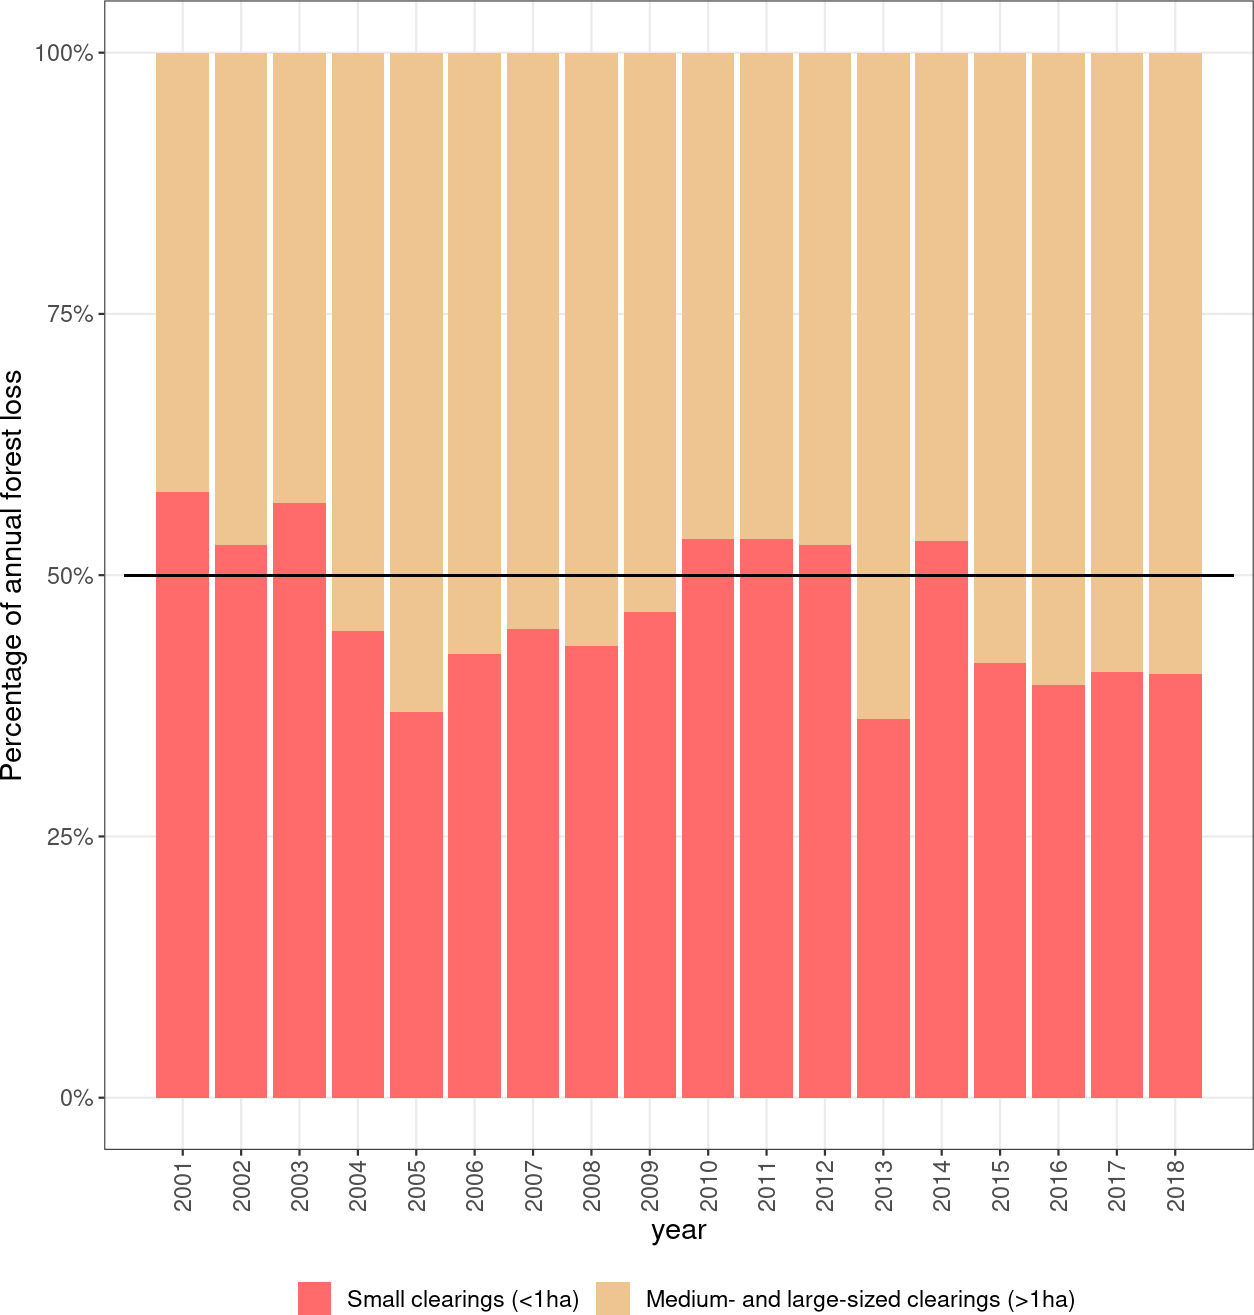
\includegraphics{img/modelling/aa-eda-ts-1} \end{center}

\begin{Shaded}
\begin{Highlighting}[]
\CommentTok{\# dev.off()}

\CommentTok{\# Tests}
\CommentTok{\# areasqm\_small\_large\_clearings \textless{}{-} readRDS(\textquotesingle{}out/deforestation\_area\_m2\_small\_and\_large\_clearings.RDS\textquotesingle{})}
\FunctionTok{sapply}\NormalTok{(areasqm\_small\_large\_clearings }\SpecialCharTok{\%\textgreater{}\%} \FunctionTok{select}\NormalTok{(}\FunctionTok{matches}\NormalTok{(}\StringTok{\textquotesingle{}PCT\textquotesingle{}}\NormalTok{)), shapiro.test) }\CommentTok{\#Not significant}
\DocumentationTok{\#\#           Small clearings (\textless{}1ha)\_PCT   }
\DocumentationTok{\#\# statistic 0.9174942                    }
\DocumentationTok{\#\# p.value   0.1167148                    }
\DocumentationTok{\#\# method    "Shapiro{-}Wilk normality test"}
\DocumentationTok{\#\# data.name "X[[i]]"                     }
\DocumentationTok{\#\#           Medium{-} and large{-}sized clearings (\textgreater{}1ha)\_PCT}
\DocumentationTok{\#\# statistic 0.9174942                                   }
\DocumentationTok{\#\# p.value   0.1167148                                   }
\DocumentationTok{\#\# method    "Shapiro{-}Wilk normality test"               }
\DocumentationTok{\#\# data.name "X[[i]]"}
\FunctionTok{with}\NormalTok{(}
\NormalTok{  areasqm\_small\_large\_clearings,}
  \FunctionTok{t.test}\NormalTok{(}\StringTok{\textasciigrave{}}\AttributeTok{Small clearings (\textless{}1ha)\_PCT}\StringTok{\textasciigrave{}}\NormalTok{, }\StringTok{\textasciigrave{}}\AttributeTok{Medium{-} and large{-}sized clearings (\textgreater{}1ha)\_PCT}\StringTok{\textasciigrave{}}\NormalTok{, }\AttributeTok{paired =}\NormalTok{ T)) }\CommentTok{\#Not significant}
\DocumentationTok{\#\# }
\DocumentationTok{\#\#  Paired t{-}test}
\DocumentationTok{\#\# }
\DocumentationTok{\#\# data:  Small clearings (\textless{}1ha)\_PCT and Medium{-} and large{-}sized clearings (\textgreater{}1ha)\_PCT}
\DocumentationTok{\#\# t = {-}2.0796, df = 17, p{-}value = 0.05301}
\DocumentationTok{\#\# alternative hypothesis: true difference in means is not equal to 0}
\DocumentationTok{\#\# 95 percent confidence interval:}
\DocumentationTok{\#\#  {-}0.1385610332  0.0009999261}
\DocumentationTok{\#\# sample estimates:}
\DocumentationTok{\#\# mean of the differences }
\DocumentationTok{\#\#             {-}0.06878055}
\DocumentationTok{\#\# Small clearings accounted for more than half of the deforested area in 7 of the first 18 years of this Century in the Dominican Republic. }

\CommentTok{\# THESE ANALYSES USE ZONAL STATISTICS FROM SIMPLE FEATURES OBJECTS}
\CommentTok{\# Four variables: absolute values per year, including cum.sum}
\NormalTok{four\_variables\_abs\_pct\_cumsum }\OtherTok{\textless{}{-}}\NormalTok{ hexzonal[, }\FunctionTok{grep}\NormalTok{(}\StringTok{\textquotesingle{}NFIRES|NCLUMPS|loss1ha\_AREASQM\textquotesingle{}}\NormalTok{, }\FunctionTok{colnames}\NormalTok{(hexzonal))] }\SpecialCharTok{\%\textgreater{}\%} 
  \FunctionTok{st\_drop\_geometry}\NormalTok{() }\SpecialCharTok{\%\textgreater{}\%} 
  \FunctionTok{pivot\_longer}\NormalTok{(}\AttributeTok{cols =} \FunctionTok{everything}\NormalTok{(), }\AttributeTok{names\_to =} \StringTok{\textquotesingle{}variable\textquotesingle{}}\NormalTok{, }\AttributeTok{values\_to =} \StringTok{\textquotesingle{}value\textquotesingle{}}\NormalTok{) }\SpecialCharTok{\%\textgreater{}\%} 
  \FunctionTok{mutate}\NormalTok{(}\AttributeTok{year =} \FunctionTok{as.numeric}\NormalTok{(}\FunctionTok{gsub}\NormalTok{(}\StringTok{\textquotesingle{}.*year([0{-}9]\{,2\}).*\textquotesingle{}}\NormalTok{, }\StringTok{\textquotesingle{}}\SpecialCharTok{\textbackslash{}\textbackslash{}}\StringTok{1\textquotesingle{}}\NormalTok{, variable)) }\SpecialCharTok{+} \DecValTok{2000}\NormalTok{) }\SpecialCharTok{\%\textgreater{}\%}
  \FunctionTok{mutate}\NormalTok{(}\AttributeTok{variable =} \FunctionTok{gsub}\NormalTok{(}\StringTok{\textquotesingle{}\_year[0{-}9]\{,2\}|year[0{-}9]\{,2\}}\SpecialCharTok{\textbackslash{}\textbackslash{}}\StringTok{.\textquotesingle{}}\NormalTok{, }\StringTok{\textquotesingle{}\textquotesingle{}}\NormalTok{, variable)) }\SpecialCharTok{\%\textgreater{}\%} 
  \FunctionTok{mutate}\NormalTok{(}\AttributeTok{variable =} \FunctionTok{case\_when}\NormalTok{(}
\NormalTok{    variable }\SpecialCharTok{==} \StringTok{\textquotesingle{}NFIRESM6\textquotesingle{}} \SpecialCharTok{\textasciitilde{}} \StringTok{\textquotesingle{}Number of MODIS M6 fire points\textquotesingle{}}\NormalTok{,}
\NormalTok{    variable }\SpecialCharTok{==} \StringTok{\textquotesingle{}NFIRESV1\textquotesingle{}} \SpecialCharTok{\textasciitilde{}} \StringTok{\textquotesingle{}Number of VIIRS V1 fire points\textquotesingle{}}\NormalTok{,}
\NormalTok{    variable }\SpecialCharTok{==} \StringTok{\textquotesingle{}NCLUMPSSMALLER1HA\textquotesingle{}} \SpecialCharTok{\textasciitilde{}} \StringTok{\textquotesingle{}Number of forest loss patches \textless{}1 Ha\textquotesingle{}}\NormalTok{,}
\NormalTok{    variable }\SpecialCharTok{==} \StringTok{\textquotesingle{}loss1ha\_AREASQM\textquotesingle{}} \SpecialCharTok{\textasciitilde{}} \StringTok{\textquotesingle{}Area of forest loss in sq. km\textquotesingle{}}
\NormalTok{  )) }\SpecialCharTok{\%\textgreater{}\%}
  \FunctionTok{replace}\NormalTok{(}\FunctionTok{is.na}\NormalTok{(.), }\DecValTok{0}\NormalTok{) }\SpecialCharTok{\%\textgreater{}\%} 
  \FunctionTok{pivot\_wider}\NormalTok{(}\AttributeTok{names\_from =} \StringTok{\textquotesingle{}variable\textquotesingle{}}\NormalTok{, }\AttributeTok{values\_from =} \StringTok{\textquotesingle{}value\textquotesingle{}}\NormalTok{, }\AttributeTok{values\_fn =}\NormalTok{ sum) }\SpecialCharTok{\%\textgreater{}\%} 
  \CommentTok{\# inner\_join(forest\_loss\_small\_clumps\_by\_year, by = \textquotesingle{}year\textquotesingle{}) \%\textgreater{}\% }
  \FunctionTok{mutate\_at}\NormalTok{(}\FunctionTok{vars}\NormalTok{(}\FunctionTok{contains}\NormalTok{(}\StringTok{\textquotesingle{}Area\textquotesingle{}}\NormalTok{)), }\SpecialCharTok{\textasciitilde{}}\NormalTok{ .}\SpecialCharTok{/}\DecValTok{1000000}\NormalTok{) }\SpecialCharTok{\%\textgreater{}\%}
  \FunctionTok{replace}\NormalTok{(}\FunctionTok{is.na}\NormalTok{(.), }\DecValTok{0}\NormalTok{) }\SpecialCharTok{\%\textgreater{}\%} 
  \FunctionTok{mutate\_at}\NormalTok{(}\FunctionTok{vars}\NormalTok{(}\SpecialCharTok{{-}}\StringTok{\textquotesingle{}year\textquotesingle{}}\NormalTok{), }\FunctionTok{funs}\NormalTok{(}\StringTok{"pct"} \OtherTok{=}\NormalTok{ .}\SpecialCharTok{/}\FunctionTok{sum}\NormalTok{(.))) }\SpecialCharTok{\%\textgreater{}\%} 
  \FunctionTok{mutate\_at}\NormalTok{(}\FunctionTok{vars}\NormalTok{(}\SpecialCharTok{{-}}\StringTok{\textquotesingle{}year\textquotesingle{}}\NormalTok{), }\FunctionTok{funs}\NormalTok{(}\StringTok{"cumsum"} \OtherTok{=} \FunctionTok{cumsum}\NormalTok{(.)))}
\NormalTok{four\_variables\_abs\_pct\_cumsum }\SpecialCharTok{\%\textgreater{}\%}
  \FunctionTok{adorn\_totals}\NormalTok{(}\AttributeTok{where =} \StringTok{\textquotesingle{}row\textquotesingle{}}\NormalTok{)}
\DocumentationTok{\#\#   year Area of forest loss in sq. km Number of MODIS M6 fire points}
\DocumentationTok{\#\#   2001                      45.65251                            351}
\DocumentationTok{\#\#   2002                      46.57304                            339}
\DocumentationTok{\#\#   2003                      44.48116                            592}
\DocumentationTok{\#\#   2004                     103.33296                            726}
\DocumentationTok{\#\#   2005                     155.73127                           1615}
\DocumentationTok{\#\#   2006                      75.61087                            837}
\DocumentationTok{\#\#   2007                      84.86968                            874}
\DocumentationTok{\#\#   2008                     116.53683                           1184}
\DocumentationTok{\#\#   2009                      72.66717                            858}
\DocumentationTok{\#\#   2010                      63.06058                            727}
\DocumentationTok{\#\#   2011                      58.09915                            977}
\DocumentationTok{\#\#   2012                      84.69065                            966}
\DocumentationTok{\#\#   2013                     103.79518                           1061}
\DocumentationTok{\#\#   2014                      78.99691                            917}
\DocumentationTok{\#\#   2015                      99.24526                            962}
\DocumentationTok{\#\#   2016                     164.00154                            492}
\DocumentationTok{\#\#   2017                     181.01097                            432}
\DocumentationTok{\#\#   2018                     101.21935                            543}
\DocumentationTok{\#\#  Total                    1679.57507                          14453}
\DocumentationTok{\#\#  Number of VIIRS V1 fire points Number of forest loss patches \textless{}1 Ha}
\DocumentationTok{\#\#                               0                               90802}
\DocumentationTok{\#\#                               0                               77007}
\DocumentationTok{\#\#                               0                               85248}
\DocumentationTok{\#\#                               0                              119844}
\DocumentationTok{\#\#                               0                              127058}
\DocumentationTok{\#\#                               0                               80934}
\DocumentationTok{\#\#                               0                              100542}
\DocumentationTok{\#\#                               0                              129162}
\DocumentationTok{\#\#                               0                               90651}
\DocumentationTok{\#\#                               0                              104346}
\DocumentationTok{\#\#                               0                               96694}
\DocumentationTok{\#\#                            4470                              135449}
\DocumentationTok{\#\#                            5326                               85798}
\DocumentationTok{\#\#                            4679                              127090}
\DocumentationTok{\#\#                            5521                              102245}
\DocumentationTok{\#\#                            3141                              151781}
\DocumentationTok{\#\#                            2649                              176204}
\DocumentationTok{\#\#                            3224                               97408}
\DocumentationTok{\#\#                           29010                             1978263}
\DocumentationTok{\#\#  Area of forest loss in sq. km\_pct Number of MODIS M6 fire points\_pct}
\DocumentationTok{\#\#                         0.02718099                         0.02428562}
\DocumentationTok{\#\#                         0.02772906                         0.02345534}
\DocumentationTok{\#\#                         0.02648358                         0.04096035}
\DocumentationTok{\#\#                         0.06152328                         0.05023179}
\DocumentationTok{\#\#                         0.09272064                         0.11174151}
\DocumentationTok{\#\#                         0.04501785                         0.05791185}
\DocumentationTok{\#\#                         0.05053045                         0.06047187}
\DocumentationTok{\#\#                         0.06938471                         0.08192071}
\DocumentationTok{\#\#                         0.04326521                         0.05936484}
\DocumentationTok{\#\#                         0.03754555                         0.05030098}
\DocumentationTok{\#\#                         0.03459157                         0.06759842}
\DocumentationTok{\#\#                         0.05042385                         0.06683733}
\DocumentationTok{\#\#                         0.06179848                         0.07341036}
\DocumentationTok{\#\#                         0.04703387                         0.06344704}
\DocumentationTok{\#\#                         0.05908950                         0.06656058}
\DocumentationTok{\#\#                         0.09764466                         0.03404138}
\DocumentationTok{\#\#                         0.10777188                         0.02988999}
\DocumentationTok{\#\#                         0.06026485                         0.03757005}
\DocumentationTok{\#\#                         1.00000000                         1.00000000}
\DocumentationTok{\#\#  Number of VIIRS V1 fire points\_pct Number of forest loss patches \textless{}1 Ha\_pct}
\DocumentationTok{\#\#                          0.00000000                              0.04589986}
\DocumentationTok{\#\#                          0.00000000                              0.03892657}
\DocumentationTok{\#\#                          0.00000000                              0.04309235}
\DocumentationTok{\#\#                          0.00000000                              0.06058042}
\DocumentationTok{\#\#                          0.00000000                              0.06422705}
\DocumentationTok{\#\#                          0.00000000                              0.04091165}
\DocumentationTok{\#\#                          0.00000000                              0.05082337}
\DocumentationTok{\#\#                          0.00000000                              0.06529061}
\DocumentationTok{\#\#                          0.00000000                              0.04582353}
\DocumentationTok{\#\#                          0.00000000                              0.05274627}
\DocumentationTok{\#\#                          0.00000000                              0.04887823}
\DocumentationTok{\#\#                          0.15408480                              0.06846865}
\DocumentationTok{\#\#                          0.18359186                              0.04337037}
\DocumentationTok{\#\#                          0.16128921                              0.06424323}
\DocumentationTok{\#\#                          0.19031368                              0.05168423}
\DocumentationTok{\#\#                          0.10827301                              0.07672438}
\DocumentationTok{\#\#                          0.09131334                              0.08907006}
\DocumentationTok{\#\#                          0.11113409                              0.04923916}
\DocumentationTok{\#\#                          1.00000000                              1.00000000}
\DocumentationTok{\#\#  Area of forest loss in sq. km\_cumsum Number of MODIS M6 fire points\_cumsum}
\DocumentationTok{\#\#                              45.65251                                   351}
\DocumentationTok{\#\#                              92.22555                                   690}
\DocumentationTok{\#\#                             136.70671                                  1282}
\DocumentationTok{\#\#                             240.03967                                  2008}
\DocumentationTok{\#\#                             395.77095                                  3623}
\DocumentationTok{\#\#                             471.38181                                  4460}
\DocumentationTok{\#\#                             556.25150                                  5334}
\DocumentationTok{\#\#                             672.78833                                  6518}
\DocumentationTok{\#\#                             745.45549                                  7376}
\DocumentationTok{\#\#                             808.51607                                  8103}
\DocumentationTok{\#\#                             866.61521                                  9080}
\DocumentationTok{\#\#                             951.30586                                 10046}
\DocumentationTok{\#\#                            1055.10104                                 11107}
\DocumentationTok{\#\#                            1134.09796                                 12024}
\DocumentationTok{\#\#                            1233.34322                                 12986}
\DocumentationTok{\#\#                            1397.34476                                 13478}
\DocumentationTok{\#\#                            1578.35573                                 13910}
\DocumentationTok{\#\#                            1679.57507                                 14453}
\DocumentationTok{\#\#                           14060.52743                                136829}
\DocumentationTok{\#\#  Number of VIIRS V1 fire points\_cumsum}
\DocumentationTok{\#\#                                      0}
\DocumentationTok{\#\#                                      0}
\DocumentationTok{\#\#                                      0}
\DocumentationTok{\#\#                                      0}
\DocumentationTok{\#\#                                      0}
\DocumentationTok{\#\#                                      0}
\DocumentationTok{\#\#                                      0}
\DocumentationTok{\#\#                                      0}
\DocumentationTok{\#\#                                      0}
\DocumentationTok{\#\#                                      0}
\DocumentationTok{\#\#                                      0}
\DocumentationTok{\#\#                                   4470}
\DocumentationTok{\#\#                                   9796}
\DocumentationTok{\#\#                                  14475}
\DocumentationTok{\#\#                                  19996}
\DocumentationTok{\#\#                                  23137}
\DocumentationTok{\#\#                                  25786}
\DocumentationTok{\#\#                                  29010}
\DocumentationTok{\#\#                                 126670}
\DocumentationTok{\#\#  Number of forest loss patches \textless{}1 Ha\_cumsum}
\DocumentationTok{\#\#                                       90802}
\DocumentationTok{\#\#                                      167809}
\DocumentationTok{\#\#                                      253057}
\DocumentationTok{\#\#                                      372901}
\DocumentationTok{\#\#                                      499959}
\DocumentationTok{\#\#                                      580893}
\DocumentationTok{\#\#                                      681435}
\DocumentationTok{\#\#                                      810597}
\DocumentationTok{\#\#                                      901248}
\DocumentationTok{\#\#                                     1005594}
\DocumentationTok{\#\#                                     1102288}
\DocumentationTok{\#\#                                     1237737}
\DocumentationTok{\#\#                                     1323535}
\DocumentationTok{\#\#                                     1450625}
\DocumentationTok{\#\#                                     1552870}
\DocumentationTok{\#\#                                     1704651}
\DocumentationTok{\#\#                                     1880855}
\DocumentationTok{\#\#                                     1978263}
\DocumentationTok{\#\#                                    17595119}
\DocumentationTok{\#\#  Area of forest loss in sq. km\_pct\_cumsum}
\DocumentationTok{\#\#                                0.02718099}
\DocumentationTok{\#\#                                0.05491005}
\DocumentationTok{\#\#                                0.08139363}
\DocumentationTok{\#\#                                0.14291691}
\DocumentationTok{\#\#                                0.23563754}
\DocumentationTok{\#\#                                0.28065540}
\DocumentationTok{\#\#                                0.33118585}
\DocumentationTok{\#\#                                0.40057056}
\DocumentationTok{\#\#                                0.44383577}
\DocumentationTok{\#\#                                0.48138132}
\DocumentationTok{\#\#                                0.51597290}
\DocumentationTok{\#\#                                0.56639675}
\DocumentationTok{\#\#                                0.62819523}
\DocumentationTok{\#\#                                0.67522909}
\DocumentationTok{\#\#                                0.73431860}
\DocumentationTok{\#\#                                0.83196326}
\DocumentationTok{\#\#                                0.93973515}
\DocumentationTok{\#\#                                1.00000000}
\DocumentationTok{\#\#                                8.37147898}
\DocumentationTok{\#\#  Number of MODIS M6 fire points\_pct\_cumsum}
\DocumentationTok{\#\#                                 0.02428562}
\DocumentationTok{\#\#                                 0.04774095}
\DocumentationTok{\#\#                                 0.08870131}
\DocumentationTok{\#\#                                 0.13893309}
\DocumentationTok{\#\#                                 0.25067460}
\DocumentationTok{\#\#                                 0.30858645}
\DocumentationTok{\#\#                                 0.36905833}
\DocumentationTok{\#\#                                 0.45097904}
\DocumentationTok{\#\#                                 0.51034387}
\DocumentationTok{\#\#                                 0.56064485}
\DocumentationTok{\#\#                                 0.62824327}
\DocumentationTok{\#\#                                 0.69508061}
\DocumentationTok{\#\#                                 0.76849097}
\DocumentationTok{\#\#                                 0.83193801}
\DocumentationTok{\#\#                                 0.89849858}
\DocumentationTok{\#\#                                 0.93253996}
\DocumentationTok{\#\#                                 0.96242995}
\DocumentationTok{\#\#                                 1.00000000}
\DocumentationTok{\#\#                                 9.46716945}
\DocumentationTok{\#\#  Number of VIIRS V1 fire points\_pct\_cumsum}
\DocumentationTok{\#\#                                  0.0000000}
\DocumentationTok{\#\#                                  0.0000000}
\DocumentationTok{\#\#                                  0.0000000}
\DocumentationTok{\#\#                                  0.0000000}
\DocumentationTok{\#\#                                  0.0000000}
\DocumentationTok{\#\#                                  0.0000000}
\DocumentationTok{\#\#                                  0.0000000}
\DocumentationTok{\#\#                                  0.0000000}
\DocumentationTok{\#\#                                  0.0000000}
\DocumentationTok{\#\#                                  0.0000000}
\DocumentationTok{\#\#                                  0.0000000}
\DocumentationTok{\#\#                                  0.1540848}
\DocumentationTok{\#\#                                  0.3376767}
\DocumentationTok{\#\#                                  0.4989659}
\DocumentationTok{\#\#                                  0.6892796}
\DocumentationTok{\#\#                                  0.7975526}
\DocumentationTok{\#\#                                  0.8888659}
\DocumentationTok{\#\#                                  1.0000000}
\DocumentationTok{\#\#                                  4.3664254}
\DocumentationTok{\#\#  Number of forest loss patches \textless{}1 Ha\_pct\_cumsum}
\DocumentationTok{\#\#                                      0.04589986}
\DocumentationTok{\#\#                                      0.08482644}
\DocumentationTok{\#\#                                      0.12791879}
\DocumentationTok{\#\#                                      0.18849920}
\DocumentationTok{\#\#                                      0.25272626}
\DocumentationTok{\#\#                                      0.29363790}
\DocumentationTok{\#\#                                      0.34446128}
\DocumentationTok{\#\#                                      0.40975189}
\DocumentationTok{\#\#                                      0.45557542}
\DocumentationTok{\#\#                                      0.50832169}
\DocumentationTok{\#\#                                      0.55719993}
\DocumentationTok{\#\#                                      0.62566858}
\DocumentationTok{\#\#                                      0.66903895}
\DocumentationTok{\#\#                                      0.73328218}
\DocumentationTok{\#\#                                      0.78496641}
\DocumentationTok{\#\#                                      0.86169079}
\DocumentationTok{\#\#                                      0.95076084}
\DocumentationTok{\#\#                                      1.00000000}
\DocumentationTok{\#\#                                      8.89422640}

\CommentTok{\# Cumulative absolute value}
\NormalTok{four\_variables\_abs\_pct\_cumsum }\SpecialCharTok{\%\textgreater{}\%}
\NormalTok{  dplyr}\SpecialCharTok{::}\FunctionTok{select}\NormalTok{(year, }\FunctionTok{matches}\NormalTok{(}\StringTok{\textquotesingle{}[a,m,s]\_cumsum\textquotesingle{}}\NormalTok{, }\AttributeTok{ignore.case =}\NormalTok{ F)) }\SpecialCharTok{\%\textgreater{}\%} 
  \FunctionTok{pivot\_longer}\NormalTok{(}\AttributeTok{cols =} \SpecialCharTok{{-}}\FunctionTok{contains}\NormalTok{(}\StringTok{\textquotesingle{}year\textquotesingle{}}\NormalTok{)) }\SpecialCharTok{\%\textgreater{}\%} 
  \FunctionTok{replace}\NormalTok{(. }\SpecialCharTok{==} \DecValTok{0}\NormalTok{, }\ConstantTok{NA}\NormalTok{) }\SpecialCharTok{\%\textgreater{}\%} 
  \FunctionTok{na.omit}\NormalTok{() }\SpecialCharTok{\%\textgreater{}\%} 
\NormalTok{  ggplot }\SpecialCharTok{+} \FunctionTok{aes}\NormalTok{(}\AttributeTok{x =}\NormalTok{ year, }\AttributeTok{y =}\NormalTok{ value) }\SpecialCharTok{+} \FunctionTok{geom\_line}\NormalTok{() }\SpecialCharTok{+}
  \FunctionTok{scale\_x\_continuous}\NormalTok{(}\AttributeTok{breaks =} \DecValTok{2001}\SpecialCharTok{:}\DecValTok{2018}\NormalTok{) }\SpecialCharTok{+} 
  \FunctionTok{scale\_y\_continuous}\NormalTok{(}\AttributeTok{labels =} \ControlFlowTok{function}\NormalTok{(y) }\FunctionTok{gsub}\NormalTok{(}\StringTok{\textquotesingle{}}\SpecialCharTok{\textbackslash{}\textbackslash{}}\StringTok{.[0]\textquotesingle{}}\NormalTok{, }\StringTok{\textquotesingle{}\textquotesingle{}}\NormalTok{, }\FunctionTok{label\_number\_si}\NormalTok{(}\AttributeTok{accuracy =} \FloatTok{0.1}\NormalTok{)(y))) }\SpecialCharTok{+}
  \FunctionTok{theme\_bw}\NormalTok{() }\SpecialCharTok{+}
  \FunctionTok{theme}\NormalTok{(}\AttributeTok{axis.text.x =} \FunctionTok{element\_text}\NormalTok{(}\AttributeTok{angle =} \DecValTok{90}\NormalTok{, }\AttributeTok{vjust =} \FloatTok{0.5}\NormalTok{), }\AttributeTok{panel.grid.minor =} \FunctionTok{element\_blank}\NormalTok{(),}
        \AttributeTok{text =} \FunctionTok{element\_text}\NormalTok{(}\AttributeTok{size =} \DecValTok{14}\NormalTok{), }\AttributeTok{aspect.ratio =} \DecValTok{1}\NormalTok{) }\SpecialCharTok{+}
  \FunctionTok{ylab}\NormalTok{(}\StringTok{\textquotesingle{}Cummulative value\textquotesingle{}}\NormalTok{) }\SpecialCharTok{+}
  \FunctionTok{facet\_wrap}\NormalTok{(}\SpecialCharTok{\textasciitilde{}}\NormalTok{ name, }\AttributeTok{scales =} \StringTok{\textquotesingle{}free\textquotesingle{}}\NormalTok{)}
\end{Highlighting}
\end{Shaded}

\begin{center}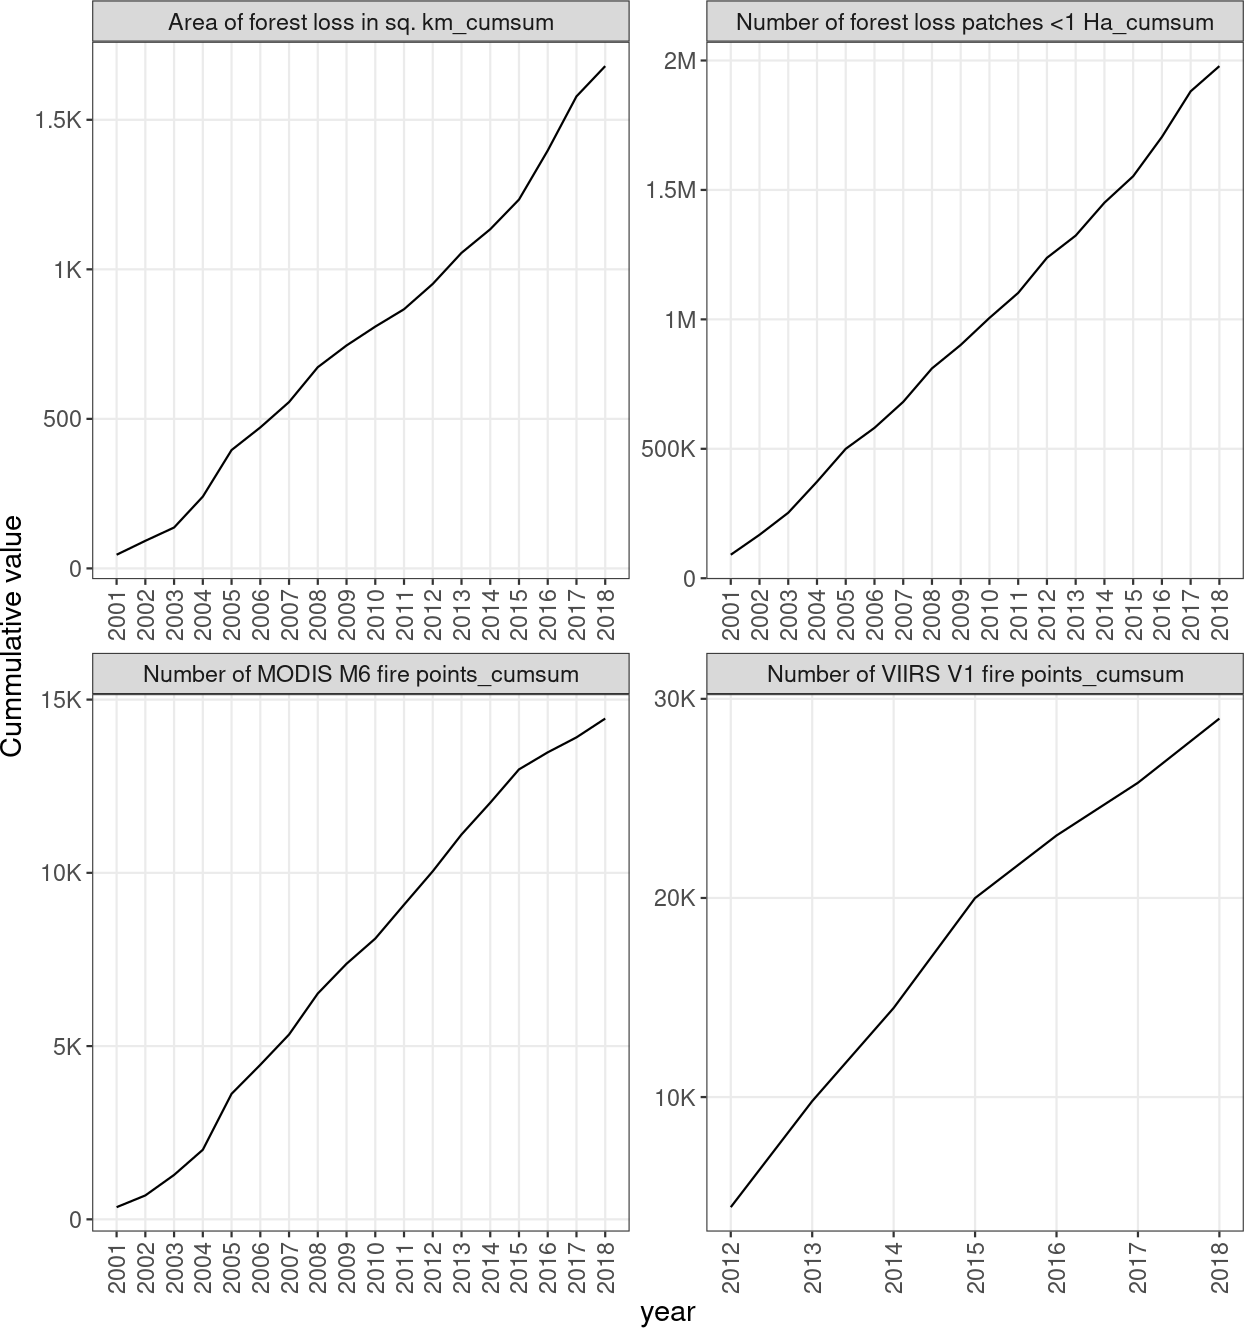
\includegraphics{img/modelling/aa-eda-ts-2} \end{center}

\begin{Shaded}
\begin{Highlighting}[]

\CommentTok{\# Cumulative proportion}
\NormalTok{four\_variables\_abs\_pct\_cumsum }\SpecialCharTok{\%\textgreater{}\%}
\NormalTok{  dplyr}\SpecialCharTok{::}\FunctionTok{select}\NormalTok{(}\FunctionTok{matches}\NormalTok{(}\StringTok{\textquotesingle{}year|pct\_cumsum\textquotesingle{}}\NormalTok{)) }\SpecialCharTok{\%\textgreater{}\%} 
  \FunctionTok{pivot\_longer}\NormalTok{(}\AttributeTok{cols =} \FunctionTok{contains}\NormalTok{(}\StringTok{\textquotesingle{}cumsum\textquotesingle{}}\NormalTok{)) }\SpecialCharTok{\%\textgreater{}\%} 
  \FunctionTok{replace}\NormalTok{(. }\SpecialCharTok{==} \DecValTok{0}\NormalTok{, }\ConstantTok{NA}\NormalTok{) }\SpecialCharTok{\%\textgreater{}\%}
  \FunctionTok{na.omit}\NormalTok{() }\SpecialCharTok{\%\textgreater{}\%} 
\NormalTok{  ggplot }\SpecialCharTok{+} \FunctionTok{aes}\NormalTok{(}\AttributeTok{x =}\NormalTok{ year, }\AttributeTok{y =}\NormalTok{ value) }\SpecialCharTok{+} \FunctionTok{geom\_line}\NormalTok{() }\SpecialCharTok{+}
  \FunctionTok{scale\_y\_continuous}\NormalTok{(}\AttributeTok{trans =} \StringTok{\textquotesingle{}exp\textquotesingle{}}\NormalTok{) }\SpecialCharTok{+}
  \FunctionTok{scale\_x\_continuous}\NormalTok{(}\AttributeTok{breaks =} \DecValTok{2001}\SpecialCharTok{:}\DecValTok{2018}\NormalTok{) }\SpecialCharTok{+} 
  \FunctionTok{theme\_bw}\NormalTok{() }\SpecialCharTok{+}
  \FunctionTok{theme}\NormalTok{(}\AttributeTok{axis.text.x =} \FunctionTok{element\_text}\NormalTok{(}\AttributeTok{angle =} \DecValTok{90}\NormalTok{, }\AttributeTok{vjust =} \FloatTok{0.5}\NormalTok{), }\AttributeTok{panel.grid.minor =} \FunctionTok{element\_blank}\NormalTok{(),}
        \AttributeTok{text =} \FunctionTok{element\_text}\NormalTok{(}\AttributeTok{size =} \DecValTok{14}\NormalTok{), }\AttributeTok{aspect.ratio =} \DecValTok{1}\NormalTok{) }\SpecialCharTok{+}
  \FunctionTok{ylab}\NormalTok{(}\StringTok{\textquotesingle{}Cummulative proportion\textquotesingle{}}\NormalTok{) }\SpecialCharTok{+}
  \FunctionTok{facet\_wrap}\NormalTok{(}\SpecialCharTok{\textasciitilde{}}\NormalTok{ name, }\AttributeTok{scales =} \StringTok{\textquotesingle{}free\_x\textquotesingle{}}\NormalTok{)}
\end{Highlighting}
\end{Shaded}

\begin{center}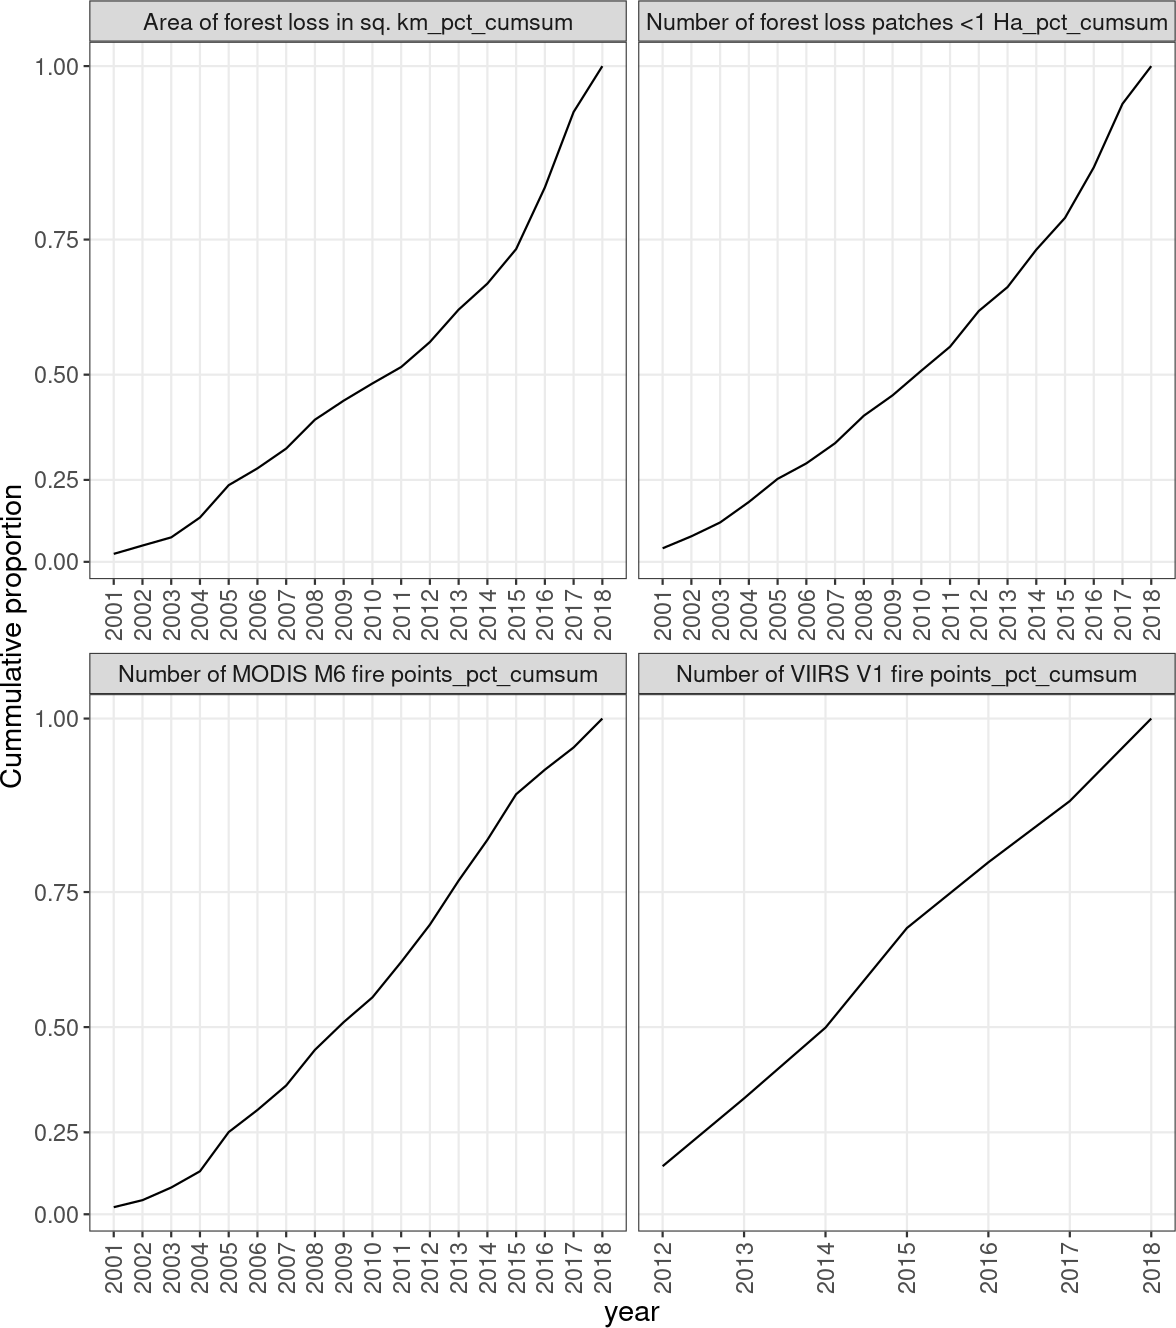
\includegraphics{img/modelling/aa-eda-ts-3} \end{center}

\begin{Shaded}
\begin{Highlighting}[]

\CommentTok{\# Absolute values non{-}cumulative}
\NormalTok{four\_variables\_abs\_pct\_cumsum }\SpecialCharTok{\%\textgreater{}\%}
\NormalTok{  dplyr}\SpecialCharTok{::}\FunctionTok{select}\NormalTok{(}\SpecialCharTok{{-}}\FunctionTok{matches}\NormalTok{(}\StringTok{\textquotesingle{}pct|cumsum\textquotesingle{}}\NormalTok{, }\AttributeTok{ignore.case =}\NormalTok{ F)) }\SpecialCharTok{\%\textgreater{}\%} 
  \FunctionTok{pivot\_longer}\NormalTok{(}\AttributeTok{cols =} \SpecialCharTok{{-}}\FunctionTok{contains}\NormalTok{(}\StringTok{\textquotesingle{}year\textquotesingle{}}\NormalTok{)) }\SpecialCharTok{\%\textgreater{}\%} 
  \FunctionTok{replace}\NormalTok{(. }\SpecialCharTok{==} \DecValTok{0}\NormalTok{, }\ConstantTok{NA}\NormalTok{) }\SpecialCharTok{\%\textgreater{}\%} 
  \FunctionTok{na.omit}\NormalTok{() }\SpecialCharTok{\%\textgreater{}\%} 
\NormalTok{  ggplot }\SpecialCharTok{+} \FunctionTok{aes}\NormalTok{(}\AttributeTok{x =}\NormalTok{ year, }\AttributeTok{y =}\NormalTok{ value) }\SpecialCharTok{+} \FunctionTok{geom\_line}\NormalTok{() }\SpecialCharTok{+}
  \FunctionTok{scale\_x\_continuous}\NormalTok{(}\AttributeTok{breaks =} \DecValTok{2001}\SpecialCharTok{:}\DecValTok{2018}\NormalTok{) }\SpecialCharTok{+} 
  \FunctionTok{scale\_y\_continuous}\NormalTok{(}\AttributeTok{trans =} \StringTok{\textquotesingle{}log\textquotesingle{}}\NormalTok{, }\AttributeTok{breaks =} \FunctionTok{pretty\_breaks}\NormalTok{(),}
                     \AttributeTok{labels =} \ControlFlowTok{function}\NormalTok{(y) }\FunctionTok{gsub}\NormalTok{(}\StringTok{\textquotesingle{}}\SpecialCharTok{\textbackslash{}\textbackslash{}}\StringTok{.[0]\textquotesingle{}}\NormalTok{, }\StringTok{\textquotesingle{}\textquotesingle{}}\NormalTok{, }\FunctionTok{label\_number\_si}\NormalTok{(}\AttributeTok{accuracy =} \FloatTok{0.1}\NormalTok{)(y))) }\SpecialCharTok{+}
  \FunctionTok{theme\_bw}\NormalTok{() }\SpecialCharTok{+}
  \FunctionTok{theme}\NormalTok{(}\AttributeTok{axis.text.x =} \FunctionTok{element\_text}\NormalTok{(}\AttributeTok{angle =} \DecValTok{90}\NormalTok{, }\AttributeTok{vjust =} \FloatTok{0.5}\NormalTok{), }\AttributeTok{panel.grid.minor =} \FunctionTok{element\_blank}\NormalTok{(),}
        \AttributeTok{text =} \FunctionTok{element\_text}\NormalTok{(}\AttributeTok{size =} \DecValTok{14}\NormalTok{), }\AttributeTok{aspect.ratio =} \DecValTok{1}\NormalTok{) }\SpecialCharTok{+}
  \FunctionTok{ylab}\NormalTok{(}\StringTok{\textquotesingle{}Value\textquotesingle{}}\NormalTok{) }\SpecialCharTok{+}
  \FunctionTok{facet\_wrap}\NormalTok{(}\SpecialCharTok{\textasciitilde{}}\NormalTok{ name, }\AttributeTok{scales =} \StringTok{\textquotesingle{}free\textquotesingle{}}\NormalTok{)}
\end{Highlighting}
\end{Shaded}

\begin{center}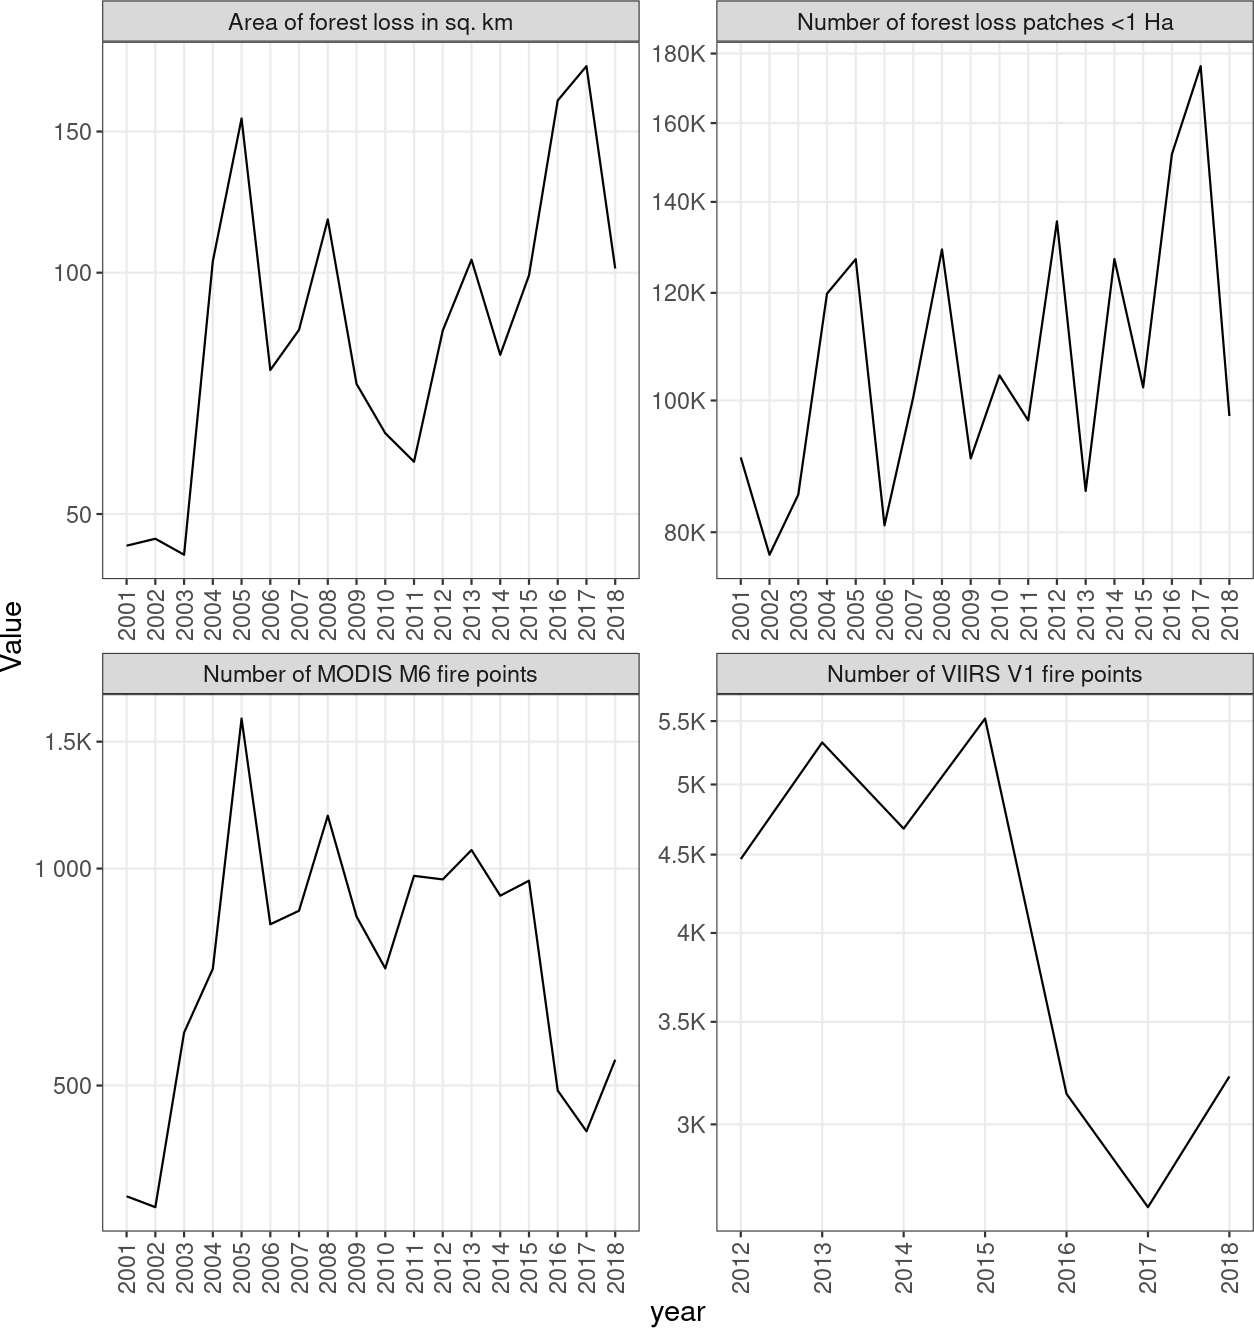
\includegraphics{img/modelling/aa-eda-ts-4} \end{center}

\begin{Shaded}
\begin{Highlighting}[]

\CommentTok{\# Three variables: summaries, plots, standard errors, confidence intervals}
\NormalTok{three\_variables\_for\_plots }\OtherTok{\textless{}{-}}\NormalTok{ hexzonalfm }\SpecialCharTok{\%\textgreater{}\%} 
  \FunctionTok{select}\NormalTok{(}\SpecialCharTok{!}\FunctionTok{matches}\NormalTok{(}\StringTok{\textquotesingle{}ENLACE|AREASQM\textquotesingle{}}\NormalTok{)) }\SpecialCharTok{\%\textgreater{}\%}
\NormalTok{  st\_drop\_geometry }\SpecialCharTok{\%\textgreater{}\%} 
  \FunctionTok{gather}\NormalTok{(variable, value) }\SpecialCharTok{\%\textgreater{}\%} 
  \FunctionTok{mutate}\NormalTok{(}\AttributeTok{year =} \FunctionTok{as.numeric}\NormalTok{(}\FunctionTok{create\_year\_from\_string}\NormalTok{(variable)) }\SpecialCharTok{+} \DecValTok{2000}\NormalTok{,}
         \AttributeTok{variable2 =} \FunctionTok{create\_variable\_name\_from\_string}\NormalTok{(variable)) }\SpecialCharTok{\%\textgreater{}\%} 
  \FunctionTok{mutate}\NormalTok{(}\AttributeTok{value =}\NormalTok{ value }\SpecialCharTok{*} \DecValTok{100}\NormalTok{) }\SpecialCharTok{\%\textgreater{}\%} 
  \FunctionTok{mutate}\NormalTok{(}\AttributeTok{variable2 =} \FunctionTok{case\_when}\NormalTok{(}
\NormalTok{    variable2 }\SpecialCharTok{==} \StringTok{\textquotesingle{}NFIRESM6PSQKM\textquotesingle{}} \SpecialCharTok{\textasciitilde{}} \StringTok{\textquotesingle{}(C)\textquotesingle{}}\NormalTok{,}
\NormalTok{    variable2 }\SpecialCharTok{==} \StringTok{\textquotesingle{}NFIRESV1PSQKM\textquotesingle{}} \SpecialCharTok{\textasciitilde{}} \StringTok{\textquotesingle{}(D)\textquotesingle{}}\NormalTok{,}
\NormalTok{    variable2 }\SpecialCharTok{==} \StringTok{\textquotesingle{}NCLUMPSSMALLER1HAPSQKM\textquotesingle{}} \SpecialCharTok{\textasciitilde{}} \StringTok{\textquotesingle{}(B)\textquotesingle{}}\NormalTok{,}
\NormalTok{    variable2 }\SpecialCharTok{==} \StringTok{\textquotesingle{}LOSSGREATER1HA\_PUA\textquotesingle{}} \SpecialCharTok{\textasciitilde{}} \StringTok{\textquotesingle{}(A)\textquotesingle{}}
\NormalTok{  ))}
\NormalTok{three\_variables\_sum }\OtherTok{\textless{}{-}} \FunctionTok{summarySE}\NormalTok{(}
\NormalTok{  three\_variables\_for\_plots }\SpecialCharTok{\%\textgreater{}\%}
  \FunctionTok{filter}\NormalTok{(}\SpecialCharTok{!}\FunctionTok{grepl}\NormalTok{(}\StringTok{\textquotesingle{}D\textquotesingle{}}\NormalTok{, variable2)),}
  \AttributeTok{measurevar=}\StringTok{"value"}\NormalTok{, }\AttributeTok{groupvars=}\FunctionTok{c}\NormalTok{(}\StringTok{\textquotesingle{}year\textquotesingle{}}\NormalTok{, }\StringTok{\textquotesingle{}variable2\textquotesingle{}}\NormalTok{))}
\NormalTok{three\_variables\_plot }\OtherTok{\textless{}{-}}\NormalTok{ three\_variables\_for\_plots }\SpecialCharTok{\%\textgreater{}\%}
  \FunctionTok{filter}\NormalTok{(}\SpecialCharTok{!}\FunctionTok{grepl}\NormalTok{(}\StringTok{\textquotesingle{}D\textquotesingle{}}\NormalTok{, variable2)) }\SpecialCharTok{\%\textgreater{}\%} 
\NormalTok{  ggplot }\SpecialCharTok{+} \FunctionTok{aes}\NormalTok{(}\AttributeTok{x =}\NormalTok{ year, }\AttributeTok{y =}\NormalTok{ value) }\SpecialCharTok{+}
  \FunctionTok{scale\_x\_continuous}\NormalTok{(}\AttributeTok{breaks =} \DecValTok{2001}\SpecialCharTok{:}\DecValTok{2018}\NormalTok{) }\SpecialCharTok{+} 
  \FunctionTok{theme\_bw}\NormalTok{() }\SpecialCharTok{+}
  \FunctionTok{theme}\NormalTok{(}\AttributeTok{axis.text.x =} \FunctionTok{element\_text}\NormalTok{(}\AttributeTok{angle =} \DecValTok{90}\NormalTok{, }\AttributeTok{vjust =} \FloatTok{0.5}\NormalTok{), }\AttributeTok{panel.grid.minor =} \FunctionTok{element\_blank}\NormalTok{(),}
        \AttributeTok{text =} \FunctionTok{element\_text}\NormalTok{(}\AttributeTok{size =} \DecValTok{14}\NormalTok{), }\AttributeTok{aspect.ratio =} \DecValTok{1}\SpecialCharTok{/}\DecValTok{3}\NormalTok{) }\SpecialCharTok{+}
  \FunctionTok{geom\_errorbar}\NormalTok{(}\AttributeTok{data =}\NormalTok{ three\_variables\_sum, }\FunctionTok{aes}\NormalTok{(}\AttributeTok{ymin =}\NormalTok{ value }\SpecialCharTok{{-}}\NormalTok{ se, }\AttributeTok{ymax =}\NormalTok{ value }\SpecialCharTok{+}\NormalTok{ se), }\AttributeTok{colour =} \StringTok{"grey30"}\NormalTok{, }\AttributeTok{width =}\NormalTok{ .}\DecValTok{3}\NormalTok{) }\SpecialCharTok{+}
  \FunctionTok{geom\_line}\NormalTok{(}\AttributeTok{data =}\NormalTok{ three\_variables\_sum) }\SpecialCharTok{+}
  \FunctionTok{geom\_point}\NormalTok{(}\AttributeTok{data =}\NormalTok{ three\_variables\_sum, }\FunctionTok{aes}\NormalTok{(}\AttributeTok{x =}\NormalTok{ year, }\AttributeTok{y =}\NormalTok{ value), }\AttributeTok{size=}\DecValTok{2}\NormalTok{, }\AttributeTok{shape=}\DecValTok{21}\NormalTok{, }\AttributeTok{fill=}\StringTok{"white"}\NormalTok{) }\SpecialCharTok{+}
  \FunctionTok{facet\_wrap}\NormalTok{(}\SpecialCharTok{\textasciitilde{}}\NormalTok{ variable2, }\AttributeTok{scales =} \StringTok{\textquotesingle{}free\_y\textquotesingle{}}\NormalTok{, }\AttributeTok{ncol =} \DecValTok{1}\NormalTok{)}
\NormalTok{three\_variables\_plot}
\end{Highlighting}
\end{Shaded}

\begin{center}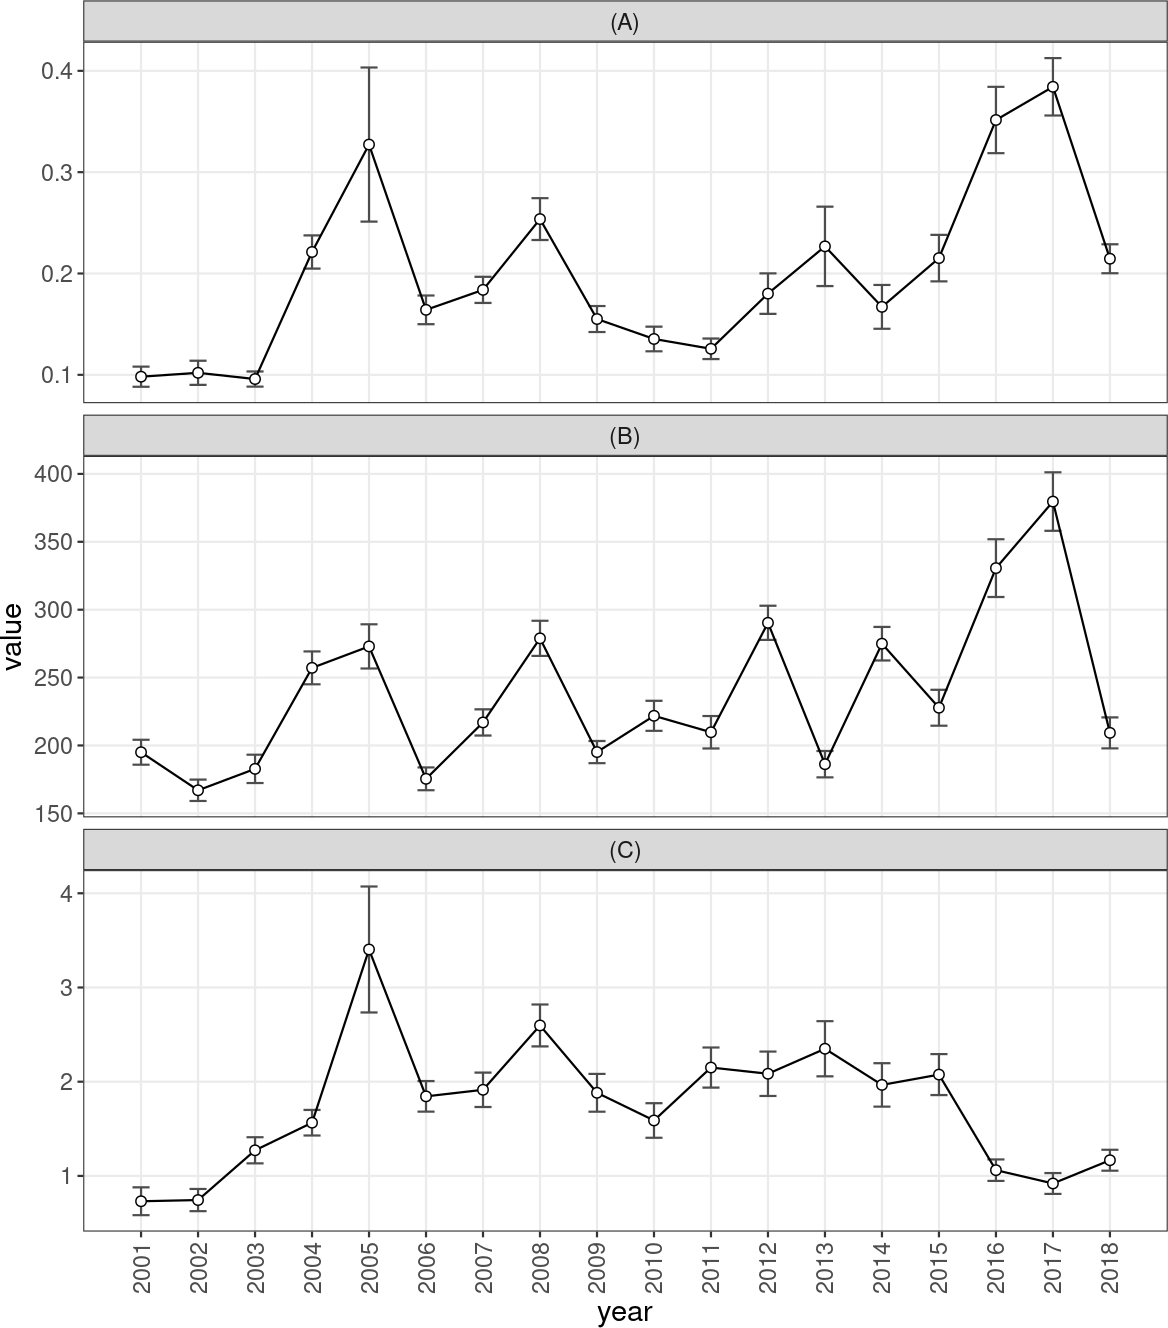
\includegraphics{img/modelling/aa-eda-ts-5} \end{center}

\begin{Shaded}
\begin{Highlighting}[]
\NormalTok{three\_variables\_plot }\SpecialCharTok{+} \FunctionTok{geom\_smooth}\NormalTok{(}\AttributeTok{method =} \StringTok{\textquotesingle{}loess\textquotesingle{}}\NormalTok{, }\AttributeTok{span =} \FloatTok{0.5}\NormalTok{)}
\end{Highlighting}
\end{Shaded}

\begin{center}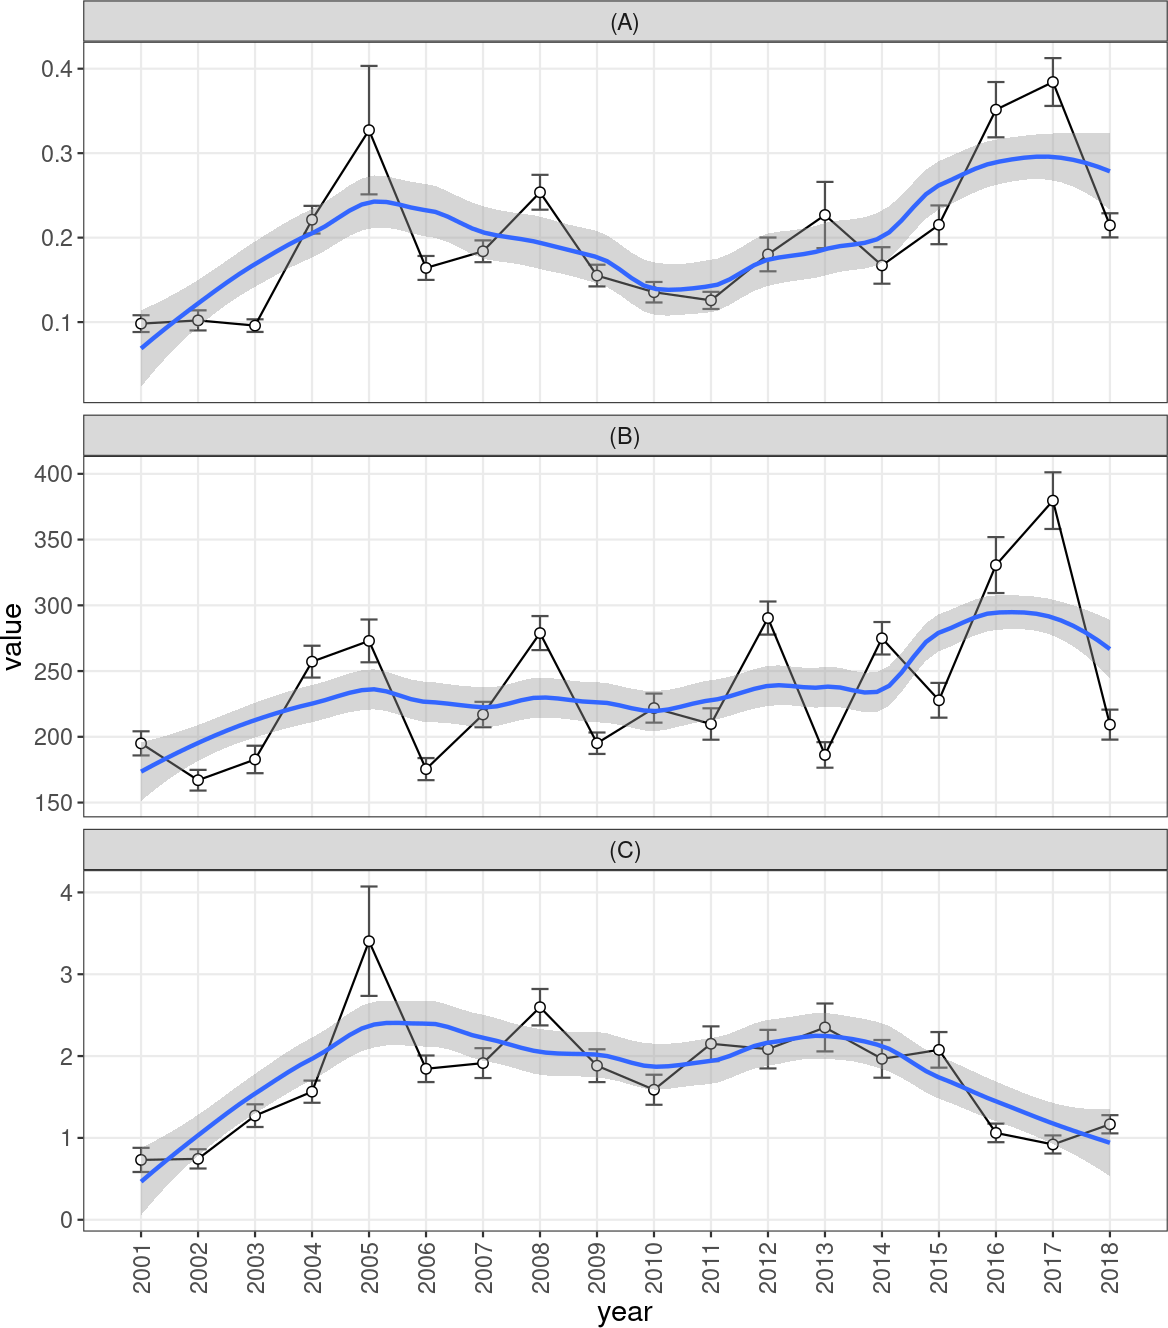
\includegraphics{img/modelling/aa-eda-ts-6} \end{center}

\begin{Shaded}
\begin{Highlighting}[]
\CommentTok{\# jpeg(\textquotesingle{}out/forest\_loss\_fire\_points\_line\_plots\_error\_bars\_2001\_2018.jpg\textquotesingle{}, width = 1800, height = 2200, res = 350)}
\CommentTok{\# dev.off()}

\CommentTok{\# Four variables: summaries, plots, standard errors, confidence intervals. Includes summary tables for the paper }
\DocumentationTok{\#\# Prepare table}
\NormalTok{four\_variables\_for\_plots }\OtherTok{\textless{}{-}}\NormalTok{ hexzonalfm }\SpecialCharTok{\%\textgreater{}\%} 
  \FunctionTok{select}\NormalTok{(}\SpecialCharTok{!}\FunctionTok{matches}\NormalTok{(}\StringTok{\textquotesingle{}ENLACE|AREASQM\textquotesingle{}}\NormalTok{)) }\SpecialCharTok{\%\textgreater{}\%}
\NormalTok{  st\_drop\_geometry }\SpecialCharTok{\%\textgreater{}\%} 
  \FunctionTok{gather}\NormalTok{(variable, value) }\SpecialCharTok{\%\textgreater{}\%} 
  \FunctionTok{mutate}\NormalTok{(}\AttributeTok{year =} \FunctionTok{as.numeric}\NormalTok{(}\FunctionTok{create\_year\_from\_string}\NormalTok{(variable)) }\SpecialCharTok{+} \DecValTok{2000}\NormalTok{,}
         \AttributeTok{variable2 =} \FunctionTok{create\_variable\_name\_from\_string}\NormalTok{(variable)) }\SpecialCharTok{\%\textgreater{}\%} 
  \FunctionTok{mutate}\NormalTok{(}\AttributeTok{value =}\NormalTok{ value }\SpecialCharTok{*} \DecValTok{100}\NormalTok{) }\SpecialCharTok{\%\textgreater{}\%} 
  \FunctionTok{mutate}\NormalTok{(}\AttributeTok{variable2 =} \FunctionTok{case\_when}\NormalTok{(}
\NormalTok{    variable2 }\SpecialCharTok{==} \StringTok{\textquotesingle{}NFIRESM6PSQKM\textquotesingle{}} \SpecialCharTok{\textasciitilde{}} \StringTok{\textquotesingle{}(C)\textquotesingle{}}\NormalTok{,}
\NormalTok{    variable2 }\SpecialCharTok{==} \StringTok{\textquotesingle{}NFIRESV1PSQKM\textquotesingle{}} \SpecialCharTok{\textasciitilde{}} \StringTok{\textquotesingle{}(D)\textquotesingle{}}\NormalTok{,}
\NormalTok{    variable2 }\SpecialCharTok{==} \StringTok{\textquotesingle{}NCLUMPSSMALLER1HAPSQKM\textquotesingle{}} \SpecialCharTok{\textasciitilde{}} \StringTok{\textquotesingle{}(B)\textquotesingle{}}\NormalTok{,}
\NormalTok{    variable2 }\SpecialCharTok{==} \StringTok{\textquotesingle{}LOSSGREATER1HA\_PUA\textquotesingle{}} \SpecialCharTok{\textasciitilde{}} \StringTok{\textquotesingle{}(A)\textquotesingle{}}
\NormalTok{  ))}
\NormalTok{four\_variables\_for\_plots}\SpecialCharTok{$}\NormalTok{year\_factor }\OtherTok{\textless{}{-}} \FunctionTok{factor}\NormalTok{(four\_variables\_for\_plots}\SpecialCharTok{$}\NormalTok{year)}
\NormalTok{four\_variables\_for\_plots}\SpecialCharTok{$}\NormalTok{decennial }\OtherTok{\textless{}{-}} \FunctionTok{cut}\NormalTok{(}
  \AttributeTok{x =}\NormalTok{ four\_variables\_for\_plots}\SpecialCharTok{$}\NormalTok{year}\DecValTok{{-}2000}\NormalTok{,}
  \AttributeTok{breaks =}\NormalTok{ breaks  }\OtherTok{\textless{}{-}} \FunctionTok{c}\NormalTok{(}\DecValTok{1}\NormalTok{, }\DecValTok{10}\NormalTok{, }\DecValTok{18}\NormalTok{), }\AttributeTok{include.lowest =}\NormalTok{ T,}
  \AttributeTok{labels =} \FunctionTok{seq\_along}\NormalTok{(breaks[}\SpecialCharTok{{-}}\DecValTok{1}\NormalTok{]))}
\NormalTok{four\_variables\_for\_plots}\SpecialCharTok{$}\NormalTok{decennial\_interval }\OtherTok{\textless{}{-}}\NormalTok{ four\_variables\_for\_plots }\SpecialCharTok{\%\textgreater{}\%}
  \FunctionTok{group\_by}\NormalTok{(decennial) }\SpecialCharTok{\%\textgreater{}\%}
  \FunctionTok{mutate}\NormalTok{(}\AttributeTok{interval =} \FunctionTok{factor}\NormalTok{(}\FunctionTok{paste}\NormalTok{(}\FunctionTok{min}\NormalTok{(year), }\FunctionTok{max}\NormalTok{(year), }\AttributeTok{sep =} \StringTok{\textquotesingle{}{-}\textquotesingle{}}\NormalTok{))) }\SpecialCharTok{\%\textgreater{}\%} 
  \FunctionTok{pull}\NormalTok{(interval)}
\NormalTok{four\_variables\_for\_plots}\SpecialCharTok{$}\NormalTok{quadrennial }\OtherTok{\textless{}{-}} \FunctionTok{cut}\NormalTok{(}
  \AttributeTok{x =}\NormalTok{ four\_variables\_for\_plots}\SpecialCharTok{$}\NormalTok{year}\DecValTok{{-}2000}\NormalTok{,}
  \AttributeTok{breaks =}\NormalTok{ breaks  }\OtherTok{\textless{}{-}} \FunctionTok{c}\NormalTok{(}\DecValTok{1}\NormalTok{, }\DecValTok{4}\NormalTok{, }\DecValTok{8}\NormalTok{, }\DecValTok{12}\NormalTok{, }\DecValTok{16}\NormalTok{, }\DecValTok{18}\NormalTok{), }\AttributeTok{include.lowest =}\NormalTok{ T,}
  \AttributeTok{labels =} \FunctionTok{seq\_along}\NormalTok{(breaks[}\SpecialCharTok{{-}}\DecValTok{1}\NormalTok{]))}
\NormalTok{four\_variables\_for\_plots}\SpecialCharTok{$}\NormalTok{quadrennial\_interval }\OtherTok{\textless{}{-}}\NormalTok{ four\_variables\_for\_plots }\SpecialCharTok{\%\textgreater{}\%}
  \FunctionTok{group\_by}\NormalTok{(quadrennial) }\SpecialCharTok{\%\textgreater{}\%}
  \FunctionTok{mutate}\NormalTok{(}\AttributeTok{interval =} \FunctionTok{factor}\NormalTok{(}\FunctionTok{paste}\NormalTok{(}\FunctionTok{min}\NormalTok{(year), }\FunctionTok{max}\NormalTok{(year), }\AttributeTok{sep =} \StringTok{\textquotesingle{}{-}\textquotesingle{}}\NormalTok{))) }\SpecialCharTok{\%\textgreater{}\%} 
  \FunctionTok{pull}\NormalTok{(interval)}
\NormalTok{four\_variables\_for\_plots}\SpecialCharTok{$}\NormalTok{triennial }\OtherTok{\textless{}{-}} \FunctionTok{cut}\NormalTok{(}
  \AttributeTok{x =}\NormalTok{ four\_variables\_for\_plots}\SpecialCharTok{$}\NormalTok{year}\DecValTok{{-}2000}\NormalTok{,}
  \AttributeTok{breaks =}\NormalTok{ breaks  }\OtherTok{\textless{}{-}} \FunctionTok{c}\NormalTok{(}\DecValTok{1}\NormalTok{, }\DecValTok{3}\NormalTok{, }\DecValTok{6}\NormalTok{, }\DecValTok{9}\NormalTok{, }\DecValTok{12}\NormalTok{, }\DecValTok{15}\NormalTok{, }\DecValTok{18}\NormalTok{), }\AttributeTok{include.lowest =}\NormalTok{ T,}
  \AttributeTok{labels =} \FunctionTok{seq\_along}\NormalTok{(breaks[}\SpecialCharTok{{-}}\DecValTok{1}\NormalTok{]))}
\NormalTok{four\_variables\_for\_plots}\SpecialCharTok{$}\NormalTok{triennial\_interval }\OtherTok{\textless{}{-}}\NormalTok{ four\_variables\_for\_plots }\SpecialCharTok{\%\textgreater{}\%}
  \FunctionTok{group\_by}\NormalTok{(triennial) }\SpecialCharTok{\%\textgreater{}\%}
  \FunctionTok{mutate}\NormalTok{(}\AttributeTok{interval =} \FunctionTok{factor}\NormalTok{(}\FunctionTok{paste}\NormalTok{(}\FunctionTok{min}\NormalTok{(year), }\FunctionTok{max}\NormalTok{(year), }\AttributeTok{sep =} \StringTok{\textquotesingle{}{-}\textquotesingle{}}\NormalTok{))) }\SpecialCharTok{\%\textgreater{}\%} 
  \FunctionTok{pull}\NormalTok{(interval)}
\NormalTok{four\_variables\_for\_plots}\SpecialCharTok{$}\NormalTok{sexennial }\OtherTok{\textless{}{-}} \FunctionTok{cut}\NormalTok{(}
  \AttributeTok{x =}\NormalTok{ four\_variables\_for\_plots}\SpecialCharTok{$}\NormalTok{year}\DecValTok{{-}2000}\NormalTok{,}
  \AttributeTok{breaks =}\NormalTok{ breaks  }\OtherTok{\textless{}{-}} \FunctionTok{c}\NormalTok{(}\DecValTok{1}\NormalTok{, }\DecValTok{6}\NormalTok{, }\DecValTok{12}\NormalTok{, }\DecValTok{18}\NormalTok{), }\AttributeTok{include.lowest =}\NormalTok{ T,}
  \AttributeTok{labels =} \FunctionTok{seq\_along}\NormalTok{(breaks[}\SpecialCharTok{{-}}\DecValTok{1}\NormalTok{]))}
\NormalTok{four\_variables\_for\_plots}\SpecialCharTok{$}\NormalTok{sexennial\_interval }\OtherTok{\textless{}{-}}\NormalTok{ four\_variables\_for\_plots }\SpecialCharTok{\%\textgreater{}\%}
  \FunctionTok{group\_by}\NormalTok{(sexennial) }\SpecialCharTok{\%\textgreater{}\%}
  \FunctionTok{mutate}\NormalTok{(}\AttributeTok{interval =} \FunctionTok{factor}\NormalTok{(}\FunctionTok{paste}\NormalTok{(}\FunctionTok{min}\NormalTok{(year), }\FunctionTok{max}\NormalTok{(year), }\AttributeTok{sep =} \StringTok{\textquotesingle{}{-}\textquotesingle{}}\NormalTok{))) }\SpecialCharTok{\%\textgreater{}\%} 
  \FunctionTok{pull}\NormalTok{(interval)}
\DocumentationTok{\#\# Years}
\NormalTok{periodic\_summaries\_yearly }\OtherTok{\textless{}{-}} \FunctionTok{periodic\_summaries}\NormalTok{(}
  \AttributeTok{source\_table =}\NormalTok{ four\_variables\_for\_plots, }\AttributeTok{measurevar =} \StringTok{\textquotesingle{}value\textquotesingle{}}\NormalTok{,}
  \AttributeTok{bins =} \StringTok{\textquotesingle{}year\_factor\textquotesingle{}}\NormalTok{, }\AttributeTok{sum\_variable =} \StringTok{\textquotesingle{}variable2\textquotesingle{}}\NormalTok{, }\AttributeTok{aspect\_ratio =} \DecValTok{1}\SpecialCharTok{/}\DecValTok{3}\NormalTok{, }\AttributeTok{smooth\_alpha =} \FloatTok{0.3}\NormalTok{,}
  \CommentTok{\# smooth\_method = \textquotesingle{}loess\textquotesingle{}, method\_args = list(degree = 0),}
  \AttributeTok{smooth\_method =} \StringTok{\textquotesingle{}gam\textquotesingle{}}\NormalTok{, }\AttributeTok{smooth\_formula =}\NormalTok{ y }\SpecialCharTok{\textasciitilde{}} \FunctionTok{s}\NormalTok{(x, }\AttributeTok{bs =} \StringTok{\textquotesingle{}ad\textquotesingle{}}\NormalTok{, }\AttributeTok{k =} \DecValTok{13}\NormalTok{),}
  \AttributeTok{smooth\_span =} \FloatTok{0.35}\NormalTok{, }\AttributeTok{labels\_angle =} \DecValTok{90}\NormalTok{, }\AttributeTok{xlab =} \StringTok{\textquotesingle{}Year\textquotesingle{}}\NormalTok{, }\AttributeTok{smooth =}\NormalTok{ T, }\AttributeTok{save =}\NormalTok{ F,}
  \AttributeTok{plot\_filename =} \StringTok{\textquotesingle{}forest\_loss\_fire\_points\_line\_plots\_error\_bars\_2001\_2018\_four\_variables.jpg\textquotesingle{}}\NormalTok{,}
  \AttributeTok{calc\_se =}\NormalTok{ F, }\AttributeTok{new\_dev =}\NormalTok{ F}
\NormalTok{)}
\end{Highlighting}
\end{Shaded}

\begin{center}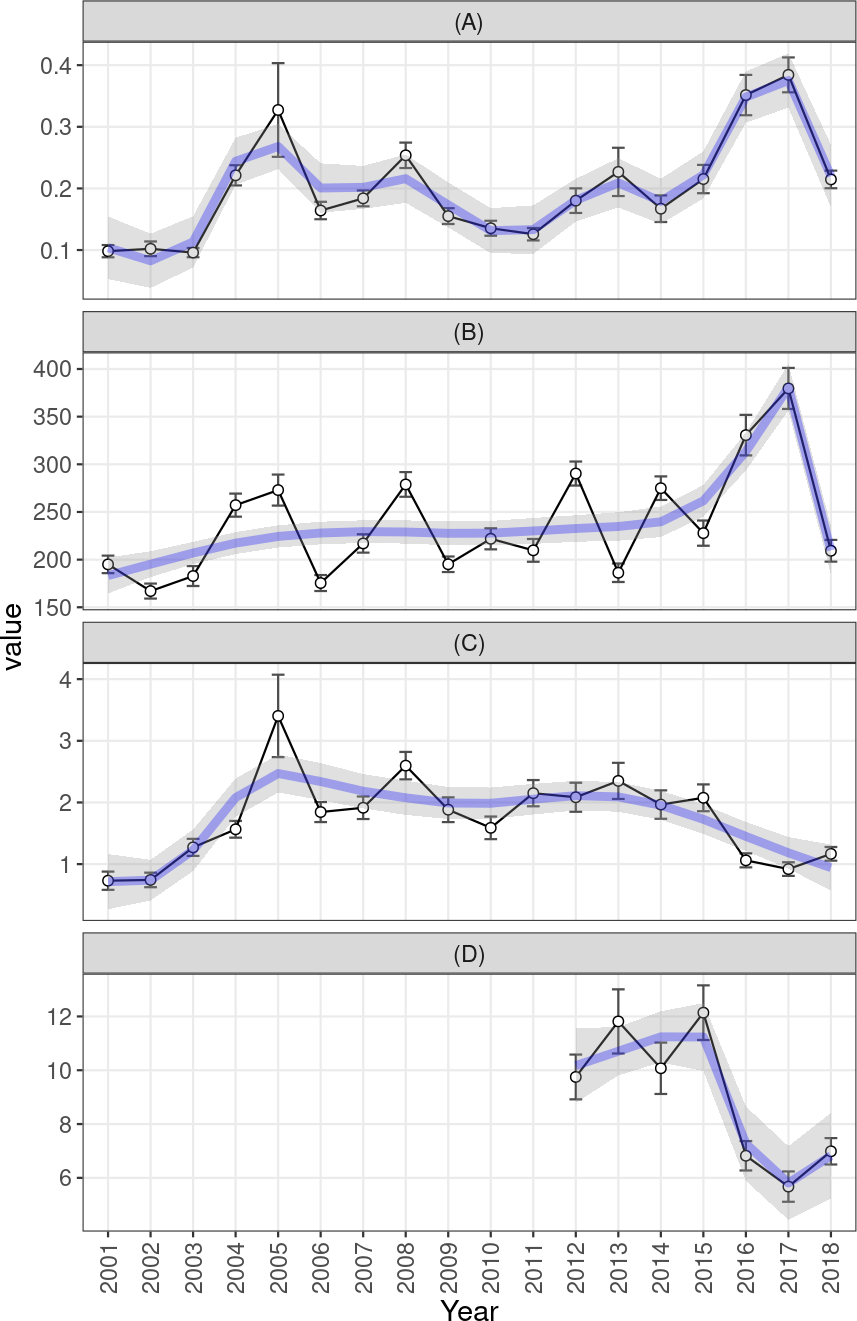
\includegraphics{img/modelling/aa-eda-ts-7} \end{center}

\begin{Shaded}
\begin{Highlighting}[]
\FunctionTok{sapply}\NormalTok{(periodic\_summaries\_yearly}\SpecialCharTok{$}\NormalTok{summaries\_print\_df[,}\SpecialCharTok{{-}}\DecValTok{1}\NormalTok{], summary)}
\DocumentationTok{\#\# $\textasciigrave{}Avg. area of forest loss in sq. km per 100 sq. km\textasciigrave{}}
\DocumentationTok{\#\#    Min. 1st Qu.  Median    Mean 3rd Qu.    Max. }
\DocumentationTok{\#\# 0.09586 0.14032 0.18200 0.20011 0.22541 0.38424 }
\DocumentationTok{\#\# }
\DocumentationTok{\#\# $\textasciigrave{}Avg. number of forest loss patches $\textless{}$1 Ha per 100 sq. km\textasciigrave{}}
\DocumentationTok{\#\#    Min. 1st Qu.  Median    Mean 3rd Qu.    Max. }
\DocumentationTok{\#\#   167.0   195.0   219.4   237.3   274.5   379.6 }
\DocumentationTok{\#\# }
\DocumentationTok{\#\# $\textasciigrave{}Avg. number of MODIS M6 fire points per 100 sq. km\textasciigrave{}}
\DocumentationTok{\#\#    Min. 1st Qu.  Median    Mean 3rd Qu.    Max. }
\DocumentationTok{\#\#  0.7312  1.1930  1.8635  1.7398  2.0823  3.4034 }
\DocumentationTok{\#\# }
\DocumentationTok{\#\# $\textasciigrave{}Avg. number of VIRS V1 fire points per 100 sq. km\textasciigrave{}}
\DocumentationTok{\#\#    Min. 1st Qu.  Median    Mean 3rd Qu.    Max.    NA\textquotesingle{}s }
\DocumentationTok{\#\#   5.676   6.905   9.751   9.038  10.944  12.139      11}
\NormalTok{periodic\_summaries\_yearly}\SpecialCharTok{$}\NormalTok{summaries\_print\_df }\SpecialCharTok{\%\textgreater{}\%}
  \FunctionTok{summarise\_at}\NormalTok{(}\FunctionTok{vars}\NormalTok{(}\SpecialCharTok{{-}}\FunctionTok{matches}\NormalTok{(}\StringTok{\textquotesingle{}\^{}year\textquotesingle{}}\NormalTok{)), psych}\SpecialCharTok{::}\NormalTok{describe, }\AttributeTok{na.rm =}\NormalTok{ T) }\SpecialCharTok{\%\textgreater{}\%}\NormalTok{ t}
\DocumentationTok{\#\#                                                                            [,1]}
\DocumentationTok{\#\# Avg. area of forest loss in sq. km per 100 sq. km.vars               1.00000000}
\DocumentationTok{\#\# Avg. area of forest loss in sq. km per 100 sq. km.n                 18.00000000}
\DocumentationTok{\#\# Avg. area of forest loss in sq. km per 100 sq. km.mean               0.20011092}
\DocumentationTok{\#\# Avg. area of forest loss in sq. km per 100 sq. km.sd                 0.08510730}
\DocumentationTok{\#\# Avg. area of forest loss in sq. km per 100 sq. km.median             0.18200213}
\DocumentationTok{\#\# Avg. area of forest loss in sq. km per 100 sq. km.trimmed            0.19511853}
\DocumentationTok{\#\# Avg. area of forest loss in sq. km per 100 sq. km.mad                0.06775677}
\DocumentationTok{\#\# Avg. area of forest loss in sq. km per 100 sq. km.min                0.09585689}
\DocumentationTok{\#\# Avg. area of forest loss in sq. km per 100 sq. km.max                0.38424317}
\DocumentationTok{\#\# Avg. area of forest loss in sq. km per 100 sq. km.range              0.28838628}
\DocumentationTok{\#\# Avg. area of forest loss in sq. km per 100 sq. km.skew               0.71665840}
\DocumentationTok{\#\# Avg. area of forest loss in sq. km per 100 sq. km.kurtosis          {-}0.54419069}
\DocumentationTok{\#\# Avg. area of forest loss in sq. km per 100 sq. km.se                 0.02005998}
\DocumentationTok{\#\# Avg. number of forest loss patches $\textless{}$1 Ha per 100 sq. km.vars       1.00000000}
\DocumentationTok{\#\# Avg. number of forest loss patches $\textless{}$1 Ha per 100 sq. km.n         18.00000000}
\DocumentationTok{\#\# Avg. number of forest loss patches $\textless{}$1 Ha per 100 sq. km.mean     237.31506716}
\DocumentationTok{\#\# Avg. number of forest loss patches $\textless{}$1 Ha per 100 sq. km.sd        57.80034547}
\DocumentationTok{\#\# Avg. number of forest loss patches $\textless{}$1 Ha per 100 sq. km.median   219.40106620}
\DocumentationTok{\#\# Avg. number of forest loss patches $\textless{}$1 Ha per 100 sq. km.trimmed  232.81564612}
\DocumentationTok{\#\# Avg. number of forest loss patches $\textless{}$1 Ha per 100 sq. km.mad       55.14388620}
\DocumentationTok{\#\# Avg. number of forest loss patches $\textless{}$1 Ha per 100 sq. km.min      166.99812254}
\DocumentationTok{\#\# Avg. number of forest loss patches $\textless{}$1 Ha per 100 sq. km.max      379.62274836}
\DocumentationTok{\#\# Avg. number of forest loss patches $\textless{}$1 Ha per 100 sq. km.range    212.62462582}
\DocumentationTok{\#\# Avg. number of forest loss patches $\textless{}$1 Ha per 100 sq. km.skew       0.84411033}
\DocumentationTok{\#\# Avg. number of forest loss patches $\textless{}$1 Ha per 100 sq. km.kurtosis  {-}0.19708272}
\DocumentationTok{\#\# Avg. number of forest loss patches $\textless{}$1 Ha per 100 sq. km.se        13.62367208}
\DocumentationTok{\#\# Avg. number of MODIS M6 fire points per 100 sq. km.vars              1.00000000}
\DocumentationTok{\#\# Avg. number of MODIS M6 fire points per 100 sq. km.n                18.00000000}
\DocumentationTok{\#\# Avg. number of MODIS M6 fire points per 100 sq. km.mean              1.73980270}
\DocumentationTok{\#\# Avg. number of MODIS M6 fire points per 100 sq. km.sd                0.69153799}
\DocumentationTok{\#\# Avg. number of MODIS M6 fire points per 100 sq. km.median            1.86350607}
\DocumentationTok{\#\# Avg. number of MODIS M6 fire points per 100 sq. km.trimmed           1.69886586}
\DocumentationTok{\#\# Avg. number of MODIS M6 fire points per 100 sq. km.mad               0.58180208}
\DocumentationTok{\#\# Avg. number of MODIS M6 fire points per 100 sq. km.min               0.73123822}
\DocumentationTok{\#\# Avg. number of MODIS M6 fire points per 100 sq. km.max               3.40335650}
\DocumentationTok{\#\# Avg. number of MODIS M6 fire points per 100 sq. km.range             2.67211829}
\DocumentationTok{\#\# Avg. number of MODIS M6 fire points per 100 sq. km.skew              0.41213467}
\DocumentationTok{\#\# Avg. number of MODIS M6 fire points per 100 sq. km.kurtosis         {-}0.27062424}
\DocumentationTok{\#\# Avg. number of MODIS M6 fire points per 100 sq. km.se                0.16299707}
\DocumentationTok{\#\# Avg. number of VIRS V1 fire points per 100 sq. km.vars               1.00000000}
\DocumentationTok{\#\# Avg. number of VIRS V1 fire points per 100 sq. km.n                  7.00000000}
\DocumentationTok{\#\# Avg. number of VIRS V1 fire points per 100 sq. km.mean               9.03751742}
\DocumentationTok{\#\# Avg. number of VIRS V1 fire points per 100 sq. km.sd                 2.56014627}
\DocumentationTok{\#\# Avg. number of VIRS V1 fire points per 100 sq. km.median             9.75085197}
\DocumentationTok{\#\# Avg. number of VIRS V1 fire points per 100 sq. km.trimmed            9.03751742}
\DocumentationTok{\#\# Avg. number of VIRS V1 fire points per 100 sq. km.mad                3.54111687}
\DocumentationTok{\#\# Avg. number of VIRS V1 fire points per 100 sq. km.min                5.67558673}
\DocumentationTok{\#\# Avg. number of VIRS V1 fire points per 100 sq. km.max               12.13930258}
\DocumentationTok{\#\# Avg. number of VIRS V1 fire points per 100 sq. km.range              6.46371585}
\DocumentationTok{\#\# Avg. number of VIRS V1 fire points per 100 sq. km.skew              {-}0.04055990}
\DocumentationTok{\#\# Avg. number of VIRS V1 fire points per 100 sq. km.kurtosis          {-}1.92615529}
\DocumentationTok{\#\# Avg. number of VIRS V1 fire points per 100 sq. km.se                 0.96764434}
\DocumentationTok{\#\# Triennials}
\FunctionTok{periodic\_summaries}\NormalTok{(}
  \AttributeTok{source\_table =}\NormalTok{ four\_variables\_for\_plots, }\AttributeTok{measurevar =} \StringTok{\textquotesingle{}value\textquotesingle{}}\NormalTok{,}
  \AttributeTok{bins =} \StringTok{\textquotesingle{}triennial\_interval\textquotesingle{}}\NormalTok{, }\AttributeTok{sum\_variable =} \StringTok{\textquotesingle{}variable2\textquotesingle{}}\NormalTok{, }\AttributeTok{aspect\_ratio =} \DecValTok{1}\SpecialCharTok{/}\DecValTok{3}\NormalTok{,}
  \AttributeTok{smooth\_span =} \FloatTok{0.7}\NormalTok{, }\AttributeTok{labels\_angle =} \DecValTok{0}\NormalTok{, }\AttributeTok{xlab =} \StringTok{\textquotesingle{}Triennial\textquotesingle{}}\NormalTok{, }\AttributeTok{smooth =}\NormalTok{ F, }\AttributeTok{save =}\NormalTok{ F,}
  \AttributeTok{plot\_filename =} \StringTok{\textquotesingle{}forest\_loss\_fire\_points\_line\_plots\_error\_bars\_2001\_2018\_four\_variables\_triennial.jpg\textquotesingle{}}\NormalTok{,}
  \AttributeTok{new\_dev =}\NormalTok{ F}
\NormalTok{)}
\end{Highlighting}
\end{Shaded}

\begin{center}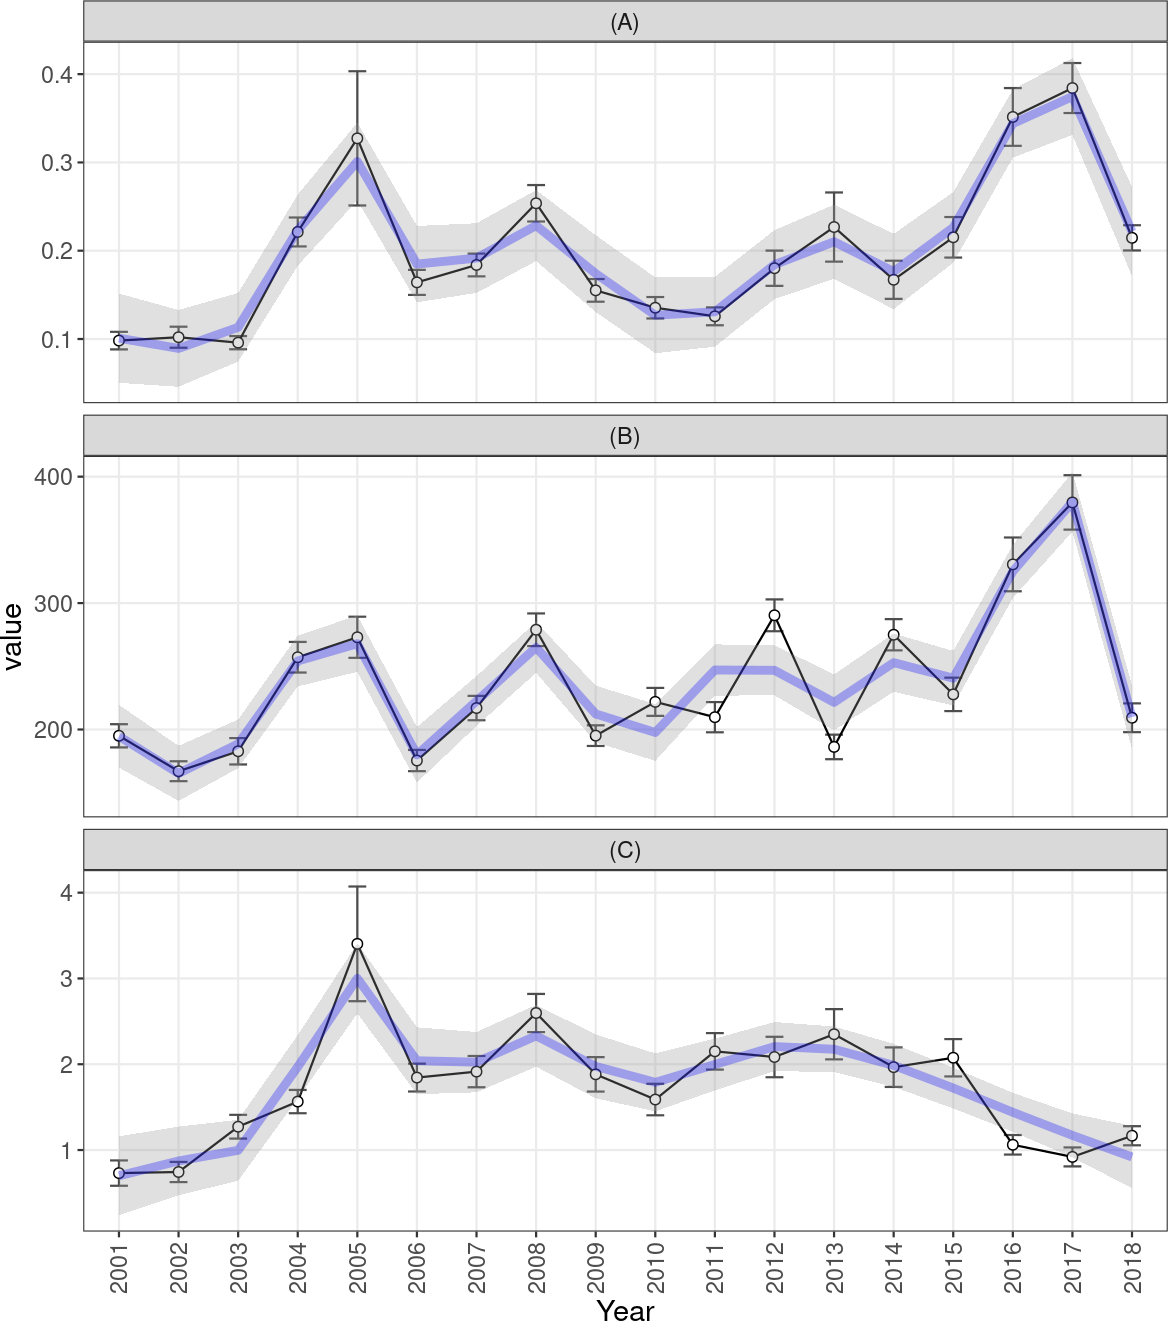
\includegraphics{img/modelling/aa-eda-ts-8} \end{center}

\begin{verbatim}
## $plot
\end{verbatim}

\begin{center}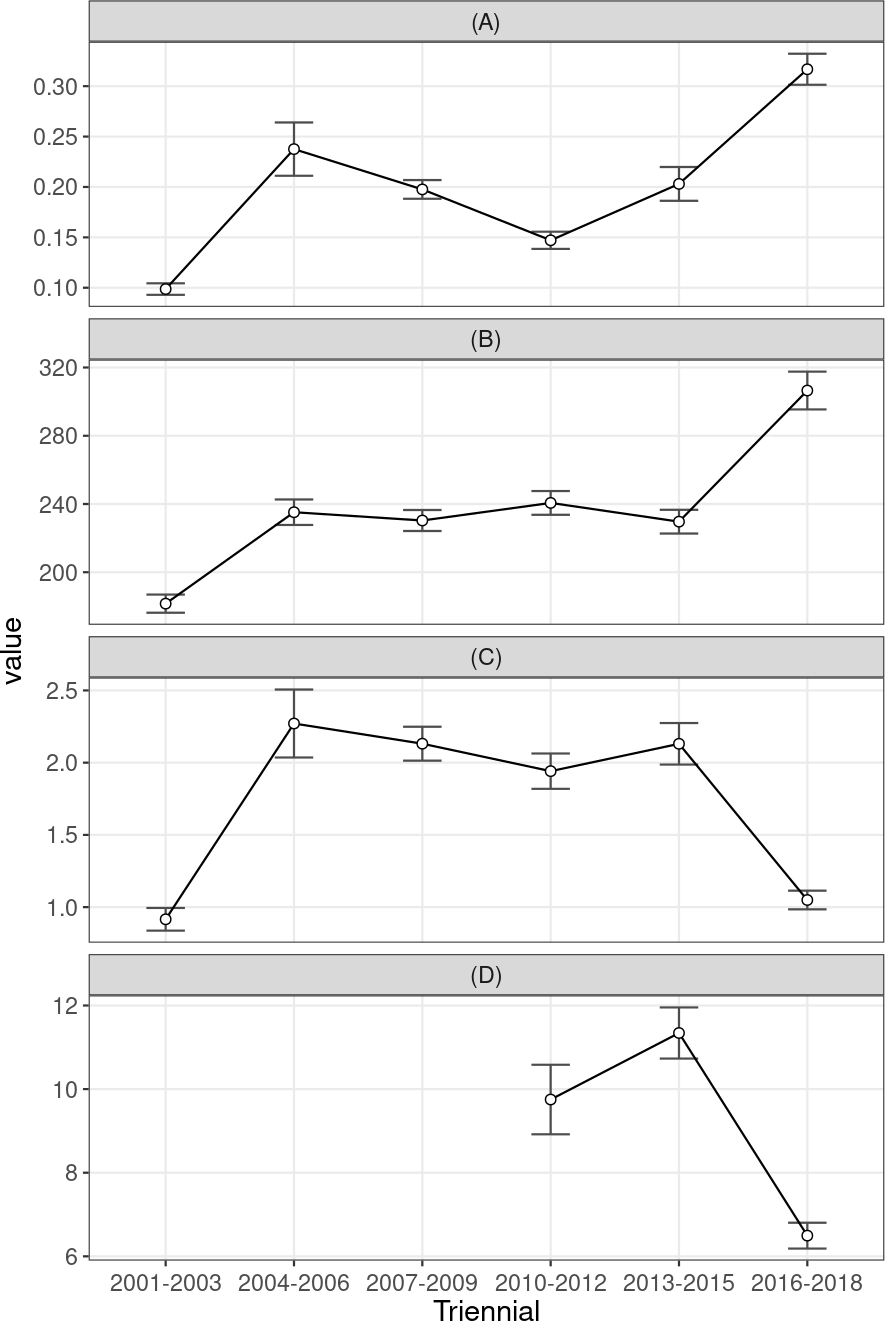
\includegraphics{img/modelling/aa-eda-ts-9} \end{center}

\begin{verbatim}
## 
## [[2]]
## 
## \begin{tabular}{l|l|l|l|l}
## \hline
## triennial\_interval & Avg. area of forest loss in sq. km per 100 sq. km & Avg. number of forest loss patches \$<\$1 Ha per 100 sq. km & Avg. number of MODIS M6 fire points per 100 sq. km & Avg. number of VIRS V1 fire points per 100 sq. km\\
## \hline
## 2001-2003 & 0.1 (0.01) & 181.59 (5.33) & 0.92 (0.08) & -\\
## \hline
## 2004-2006 & 0.24 (0.03) & 235.18 (7.47) & 2.27 (0.24) & -\\
## \hline
## 2007-2009 & 0.2 (0.01) & 230.33 (6.15) & 2.13 (0.12) & -\\
## \hline
## 2010-2012 & 0.15 (0.01) & 240.63 (6.97) & 1.94 (0.12) & 9.75 (0.83)\\
## \hline
## 2013-2015 & 0.2 (0.02) & 229.65 (6.96) & 2.13 (0.14) & 11.34 (0.61)\\
## \hline
## 2016-2018 & 0.32 (0.02) & 306.5 (11.08) & 1.05 (0.06) & 6.5 (0.31)\\
## \hline
## \end{tabular}
## 
## $summaries_print_df
## # A tibble: 6 x 5
##   triennial_interval `Avg. area of fore~ `Avg. number of for~ `Avg. number of M~
##   <fct>              <chr>               <chr>                <chr>             
## 1 2001-2003          0.1 (0.01)          181.59 (5.33)        0.92 (0.08)       
## 2 2004-2006          0.24 (0.03)         235.18 (7.47)        2.27 (0.24)       
## 3 2007-2009          0.2 (0.01)          230.33 (6.15)        2.13 (0.12)       
## 4 2010-2012          0.15 (0.01)         240.63 (6.97)        1.94 (0.12)       
## 5 2013-2015          0.2 (0.02)          229.65 (6.96)        2.13 (0.14)       
## 6 2016-2018          0.32 (0.02)         306.5 (11.08)        1.05 (0.06)       
## # ... with 1 more variable:
## #   Avg. number of VIRS V1 fire points per 100 sq. km <chr>
## Quadrennials
periodic_summaries(
  source_table = four_variables_for_plots, measurevar = 'value',
  bins = 'quadrennial_interval', sum_variable = 'variable2', aspect_ratio = 1/3,
  smooth_span = 0.7, labels_angle = 0, xlab = 'Quadrennial', smooth = F, save = F,
  plot_filename = 'forest_loss_fire_points_line_plots_error_bars_2001_2018_four_variables_quadrennial.jpg',
  new_dev = F
)
\end{verbatim}

\begin{center}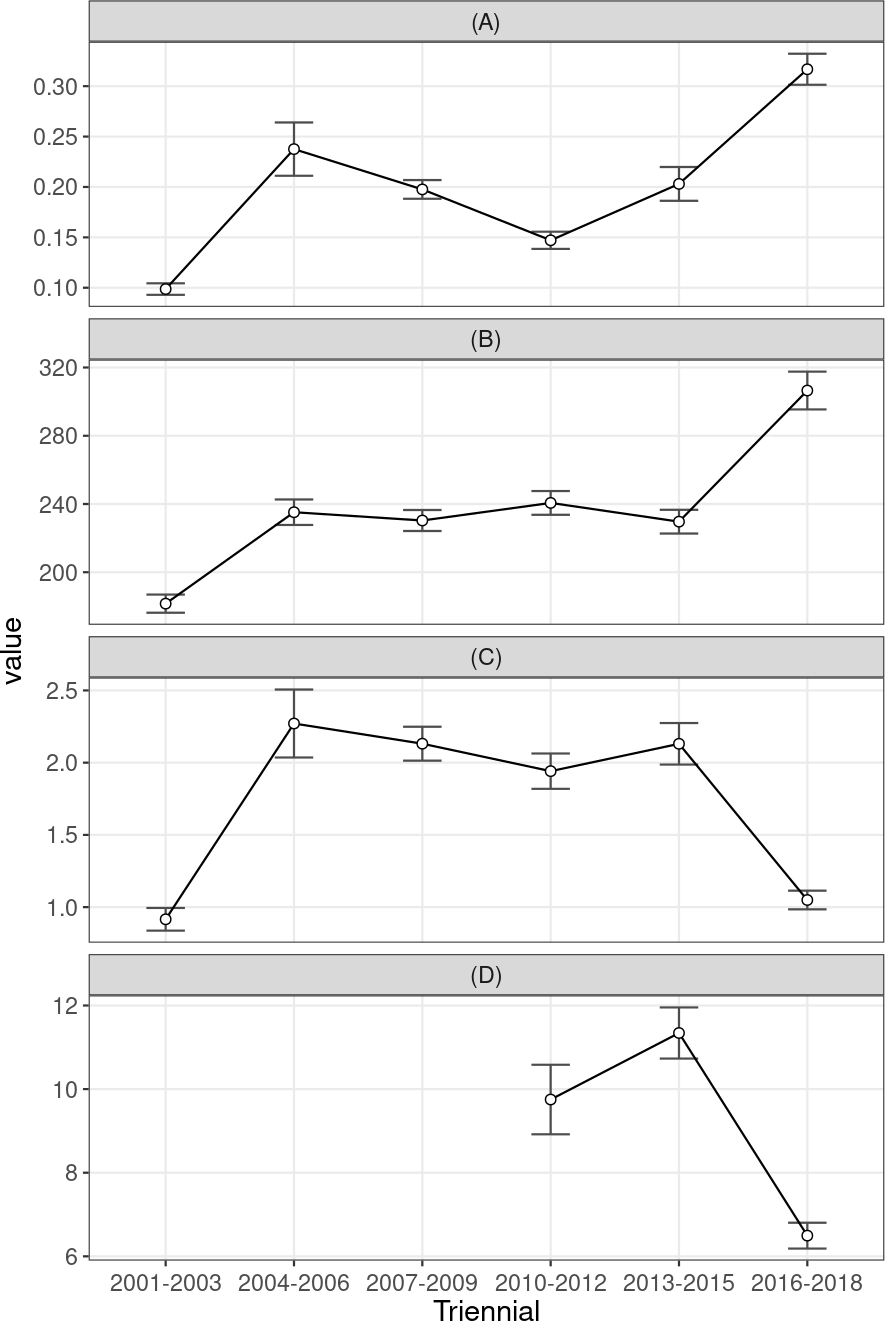
\includegraphics{img/modelling/aa-eda-ts-10} \end{center}

\begin{verbatim}
## $plot
\end{verbatim}

\begin{center}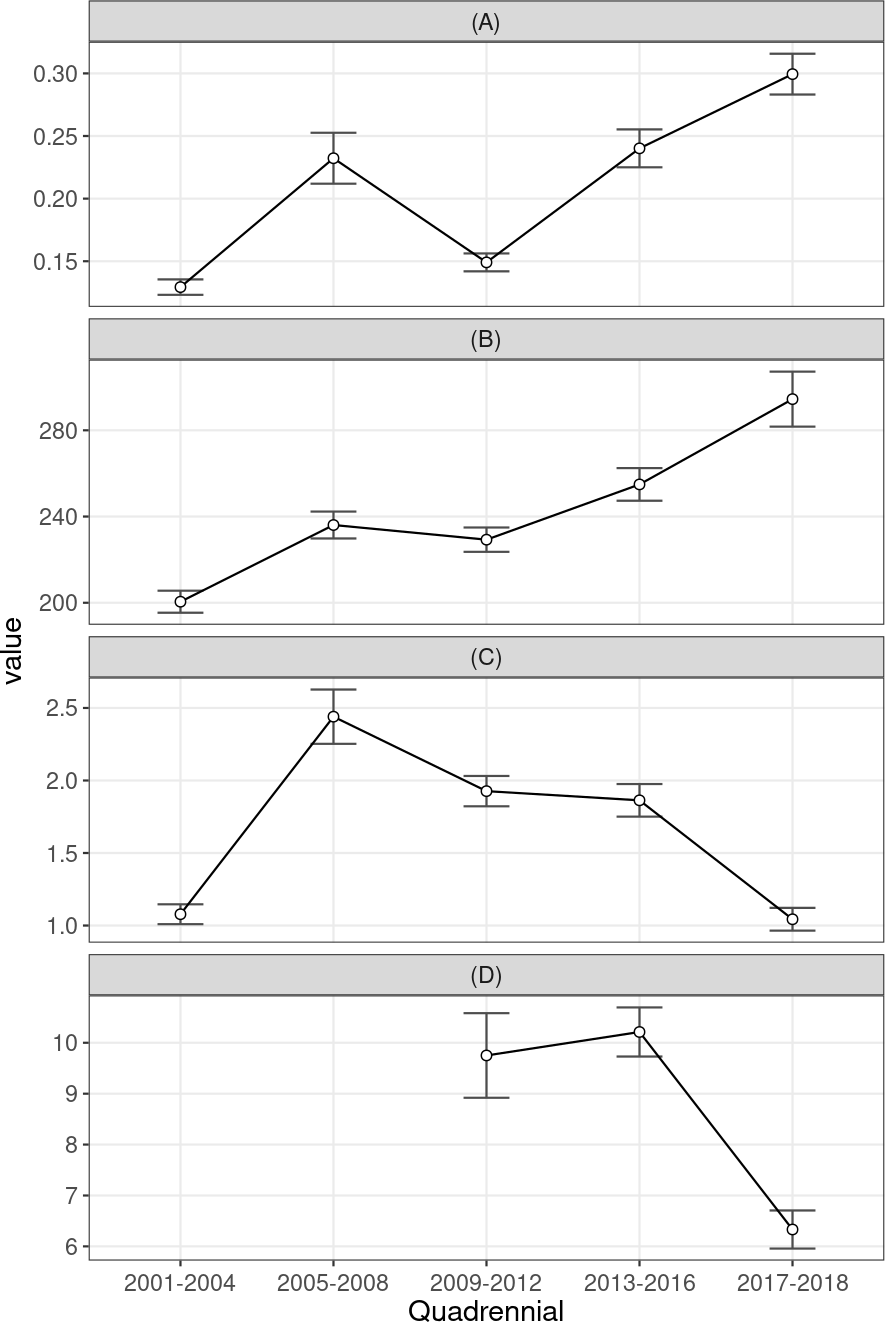
\includegraphics{img/modelling/aa-eda-ts-11} \end{center}

\begin{verbatim}
## 
## [[2]]
## 
## \begin{tabular}{l|l|l|l|l}
## \hline
## quadrennial\_interval & Avg. area of forest loss in sq. km per 100 sq. km & Avg. number of forest loss patches \$<\$1 Ha per 100 sq. km & Avg. number of MODIS M6 fire points per 100 sq. km & Avg. number of VIRS V1 fire points per 100 sq. km\\
## \hline
## 2001-2004 & 0.13 (0.01) & 200.49 (5.12) & 1.08 (0.07) & -\\
## \hline
## 2005-2008 & 0.23 (0.02) & 236.06 (6.24) & 2.44 (0.19) & -\\
## \hline
## 2009-2012 & 0.15 (0.01) & 229.26 (5.64) & 1.93 (0.1) & 9.75 (0.83)\\
## \hline
## 2013-2016 & 0.24 (0.02) & 254.89 (7.57) & 1.86 (0.11) & 10.21 (0.48)\\
## \hline
## 2017-2018 & 0.3 (0.02) & 294.45 (12.75) & 1.04 (0.08) & 6.33 (0.37)\\
## \hline
## \end{tabular}
## 
## $summaries_print_df
## # A tibble: 5 x 5
##   quadrennial_interval `Avg. area of fore~ `Avg. number of f~ `Avg. number of M~
##   <fct>                <chr>               <chr>              <chr>             
## 1 2001-2004            0.13 (0.01)         200.49 (5.12)      1.08 (0.07)       
## 2 2005-2008            0.23 (0.02)         236.06 (6.24)      2.44 (0.19)       
## 3 2009-2012            0.15 (0.01)         229.26 (5.64)      1.93 (0.1)        
## 4 2013-2016            0.24 (0.02)         254.89 (7.57)      1.86 (0.11)       
## 5 2017-2018            0.3 (0.02)          294.45 (12.75)     1.04 (0.08)       
## # ... with 1 more variable:
## #   Avg. number of VIRS V1 fire points per 100 sq. km <chr>

# Drawing results
periodic_summaries(
  source_table = four_variables_for_plots %>% filter(!variable2 == '(D)') %>%  mutate(variable2 = case_when(
    variable2 == '(C)' ~ 'C. Number of MODIS M6 fire points per 100 sq. km',
    variable2 == '(B)' ~ 'B. Number of small clearings (<1 ha) per 100 sq. km',
    variable2 == '(A)' ~ 'A. Area of forest loss in sq. km per 100 sq. km'
  )),
  measurevar = 'value',
  bins = 'quadrennial_interval', sum_variable = 'variable2', aspect_ratio = 1/2,
  smooth_span = 0.7, labels_angle = 0, xlab = 'Quadrennial', smooth = F, save = F,
  plot_filename = 'forest_loss_fire_points_line_plots_error_bars_2001_2018_four_variables_quadrennial.jpg',
  calc_se = F, new_dev = F
)
\end{verbatim}

\begin{center}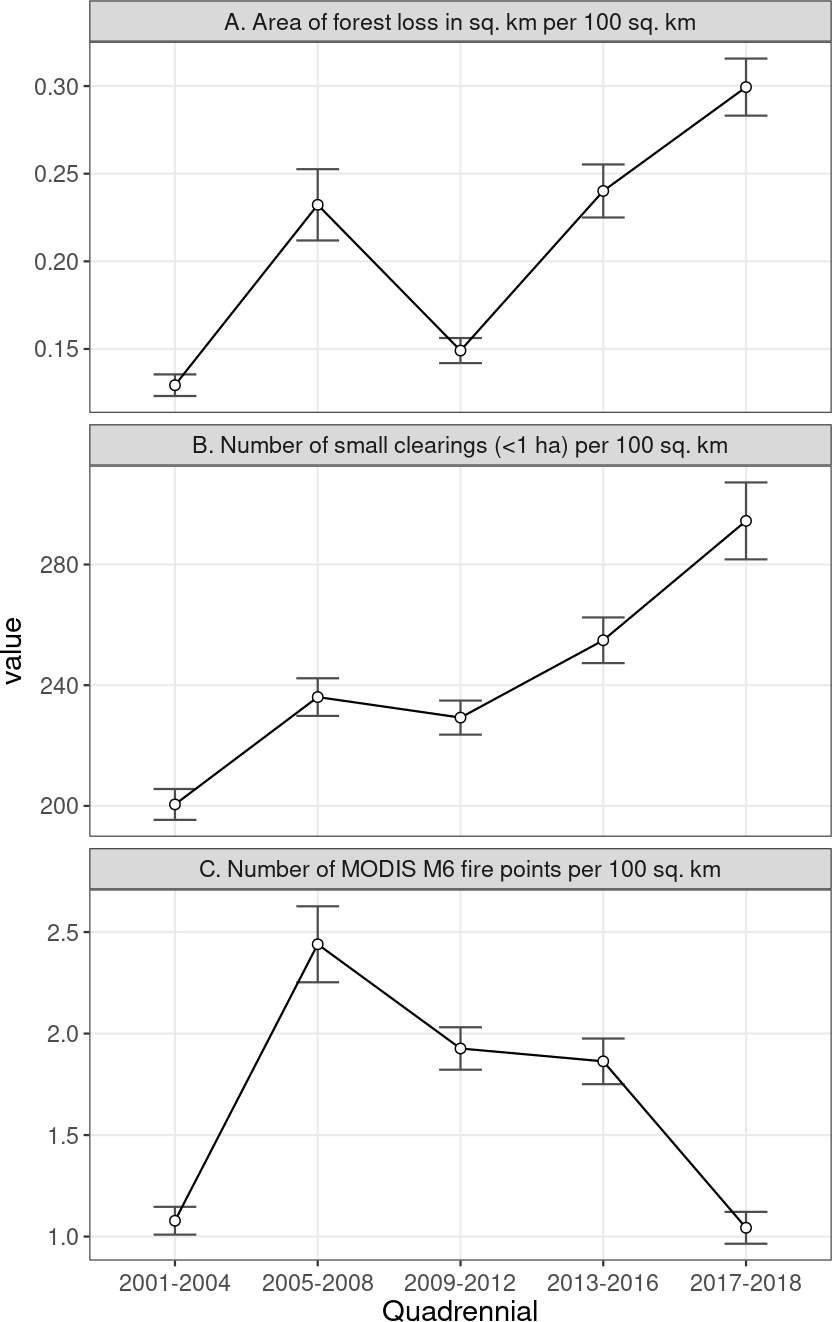
\includegraphics{img/modelling/aa-eda-ts-12} \end{center}

\begin{verbatim}
## $plot
\end{verbatim}

\begin{center}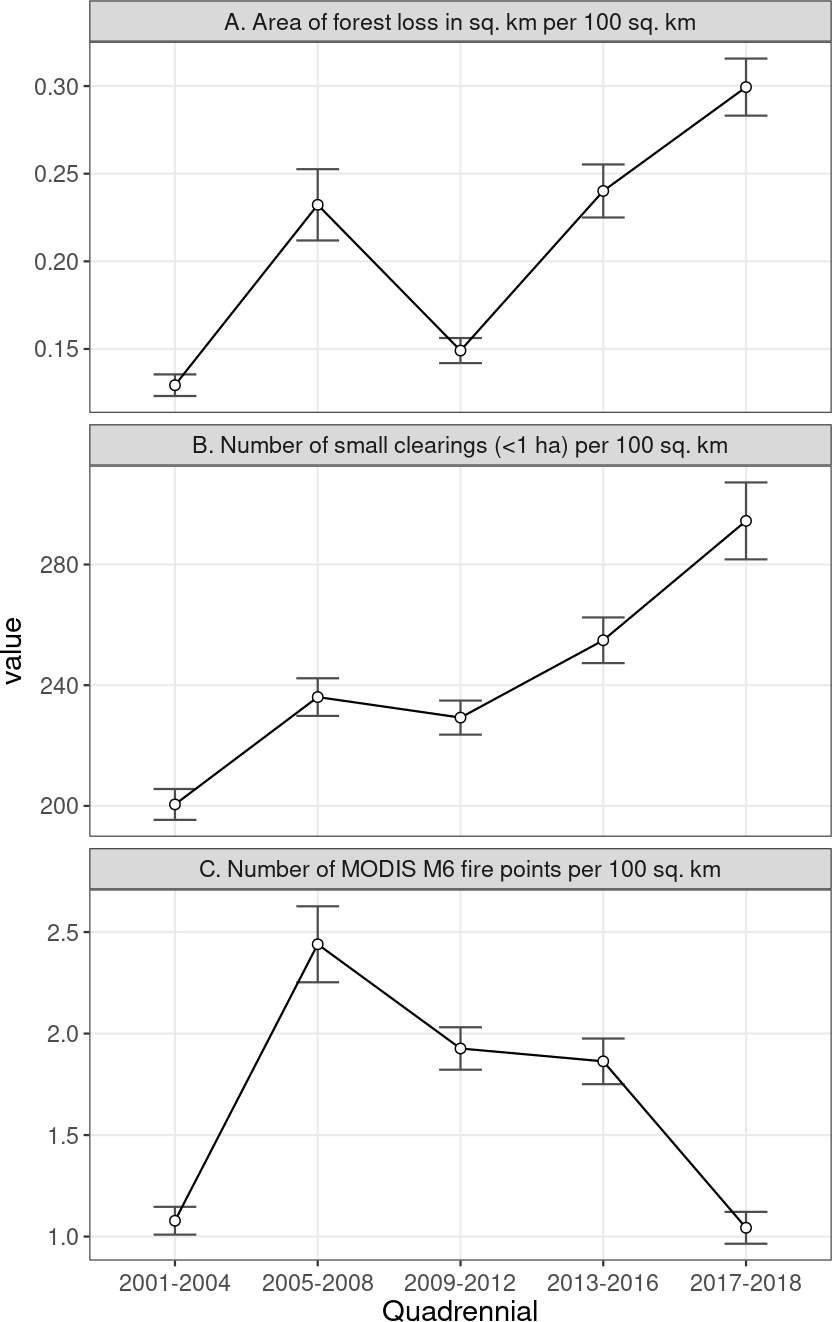
\includegraphics{img/modelling/aa-eda-ts-13} \end{center}

\begin{verbatim}
## 
## [[2]]
## 
## \begin{tabular}{l|l}
## \hline
## quadrennial\_interval & NA\\
## \hline
## 2001-2004 & 0.1293251, 200.4858820, 1.0780220\\
## \hline
## 2005-2008 & 0.2322423, 236.0592956, 2.4397988\\
## \hline
## 2009-2012 & 0.1490862, 229.2587650, 1.9264740\\
## \hline
## 2013-2016 & 0.2401406, 254.8880517, 1.8631714\\
## \hline
## 2017-2018 & 0.2994098, 294.4516158, 1.0432918\\
## \hline
## \end{tabular}
## 
## $summaries_print_df
## # A tibble: 5 x 2
##   quadrennial_interval `NA`     
##   <fct>                <list>   
## 1 2001-2004            <dbl [3]>
## 2 2005-2008            <dbl [3]>
## 3 2009-2012            <dbl [3]>
## 4 2013-2016            <dbl [3]>
## 5 2017-2018            <dbl [3]>
# In the Dominican Republic, by four-year periods from 2001 to 2018, both the area of forest loss (top) and the number of small clearings (middle) per 100 sq. km, increased since 2013 WITHOUT the help of fire (bottom). This is a worrisome pattern
periodic_summaries(
  source_table = four_variables_for_plots %>% filter(!variable2 == '(D)') %>%  mutate(variable2 = case_when(
    variable2 == '(C)' ~ 'Número de puntos de calor/fuegos MODIS por cada 100 km cuad.',
    variable2 == '(B)' ~ 'Número de parches de aclareo (<1 ha) por cada 100 km cuad.',
    variable2 == '(A)' ~ 'Área de pérdida de bosque, en km cuad., por cada 100 km cuad.'
  )),
  measurevar = 'value',
  bins = 'quadrennial_interval', sum_variable = 'variable2', aspect_ratio = 1/2,
  smooth_span = 0.7, labels_angle = 0, xlab = 'Quadrennial', smooth = F, save = F,
  plot_filename = 'forest_loss_fire_points_line_plots_error_bars_2001_2018_four_variables_quadrennial.jpg',
  calc_se = F, new_dev = F
)
\end{verbatim}

\begin{center}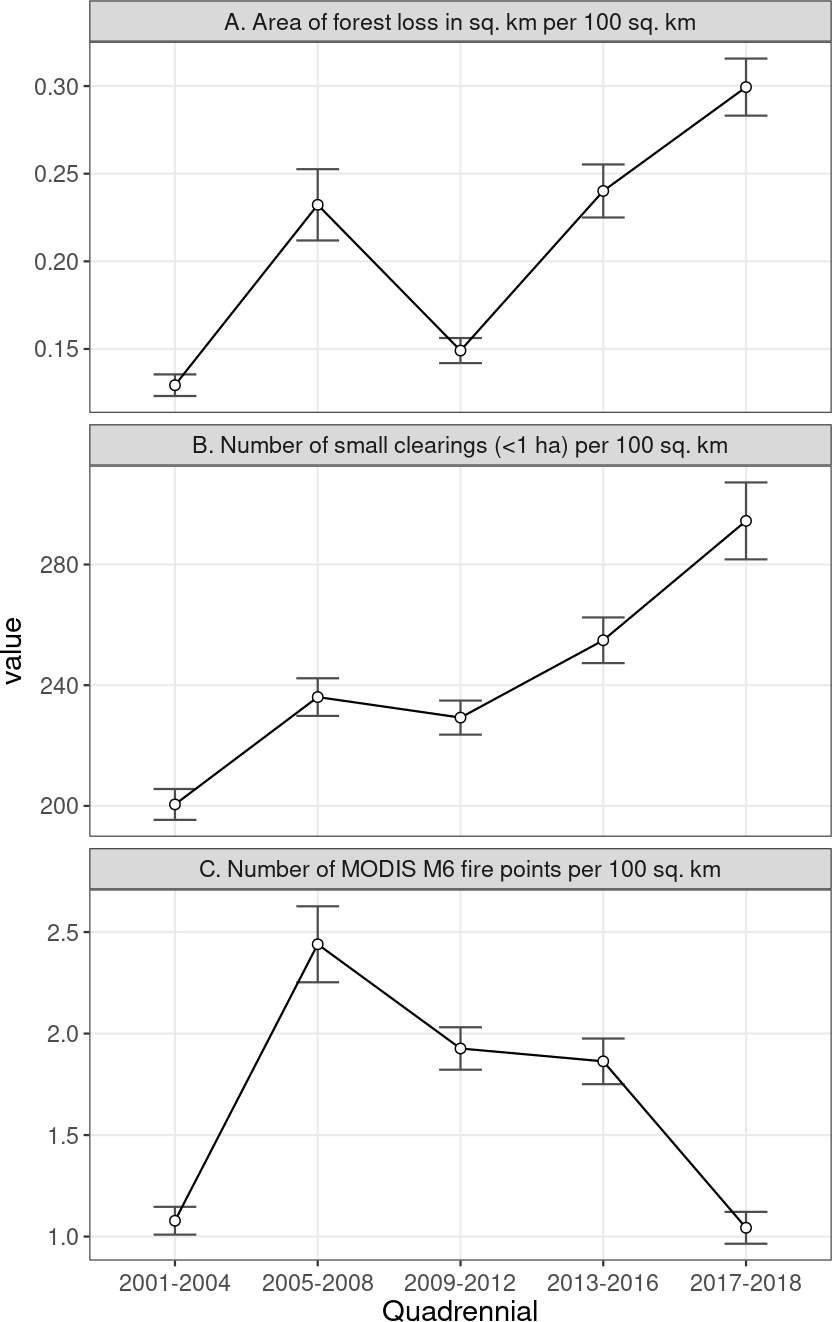
\includegraphics{img/modelling/aa-eda-ts-14} \end{center}

\begin{verbatim}
## $plot
\end{verbatim}

\begin{center}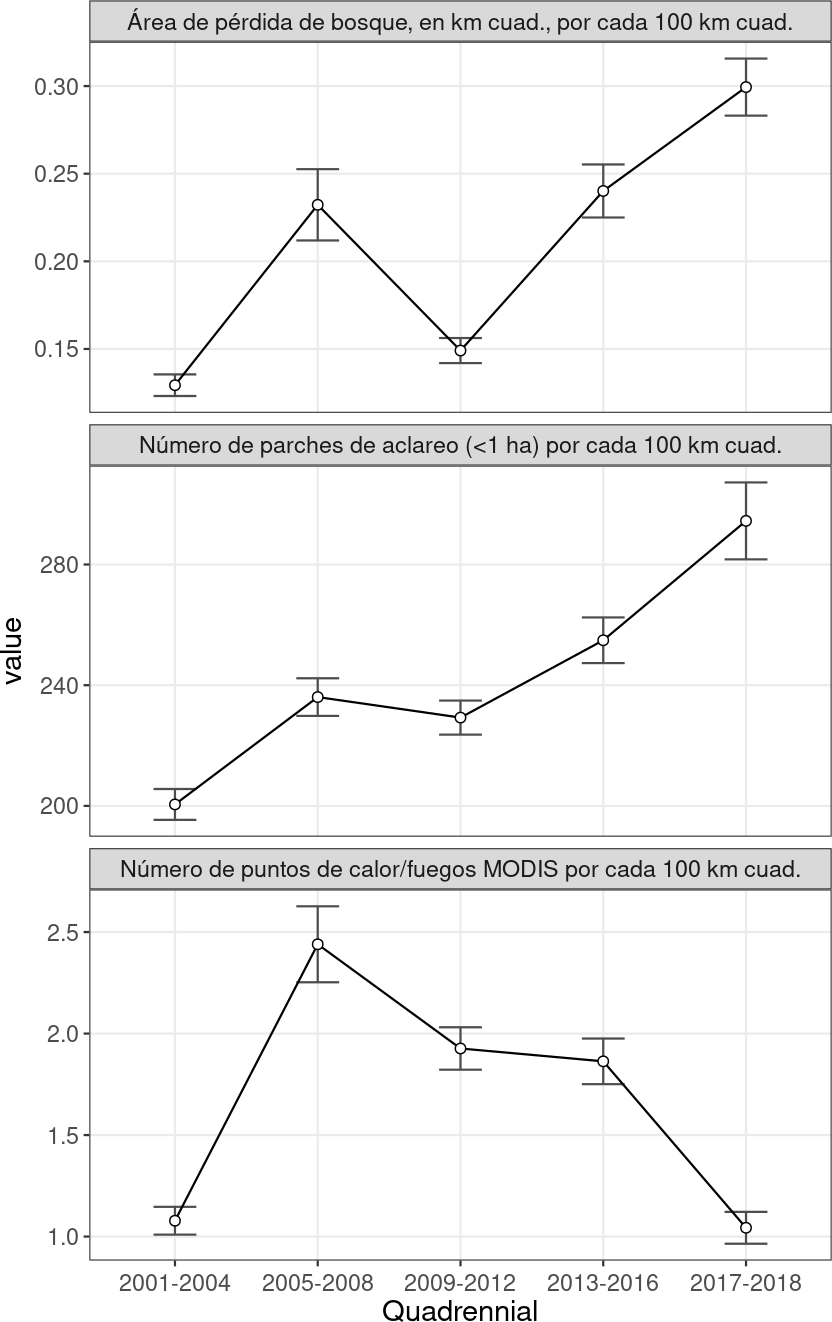
\includegraphics{img/modelling/aa-eda-ts-15} \end{center}

\begin{verbatim}
## 
## [[2]]
## 
## \begin{tabular}{l|l}
## \hline
## quadrennial\_interval & NA\\
## \hline
## 2001-2004 & 0.1293251, 200.4858820, 1.0780220\\
## \hline
## 2005-2008 & 0.2322423, 236.0592956, 2.4397988\\
## \hline
## 2009-2012 & 0.1490862, 229.2587650, 1.9264740\\
## \hline
## 2013-2016 & 0.2401406, 254.8880517, 1.8631714\\
## \hline
## 2017-2018 & 0.2994098, 294.4516158, 1.0432918\\
## \hline
## \end{tabular}
## 
## $summaries_print_df
## # A tibble: 5 x 2
##   quadrennial_interval `NA`     
##   <fct>                <list>   
## 1 2001-2004            <dbl [3]>
## 2 2005-2008            <dbl [3]>
## 3 2009-2012            <dbl [3]>
## 4 2013-2016            <dbl [3]>
## 5 2017-2018            <dbl [3]>

## Sexennials
periodic_summaries(
  source_table = four_variables_for_plots, measurevar = 'value',
  bins = 'sexennial_interval', sum_variable = 'variable2', aspect_ratio = 1/3,
  smooth_span = 0.7, labels_angle = 0, xlab = 'Sexennial', smooth = F, save = F,
  plot_filename = 'forest_loss_fire_points_line_plots_error_bars_2001_2018_four_variables_sexennial.jpg',
  new_dev = F
)
\end{verbatim}

\begin{center}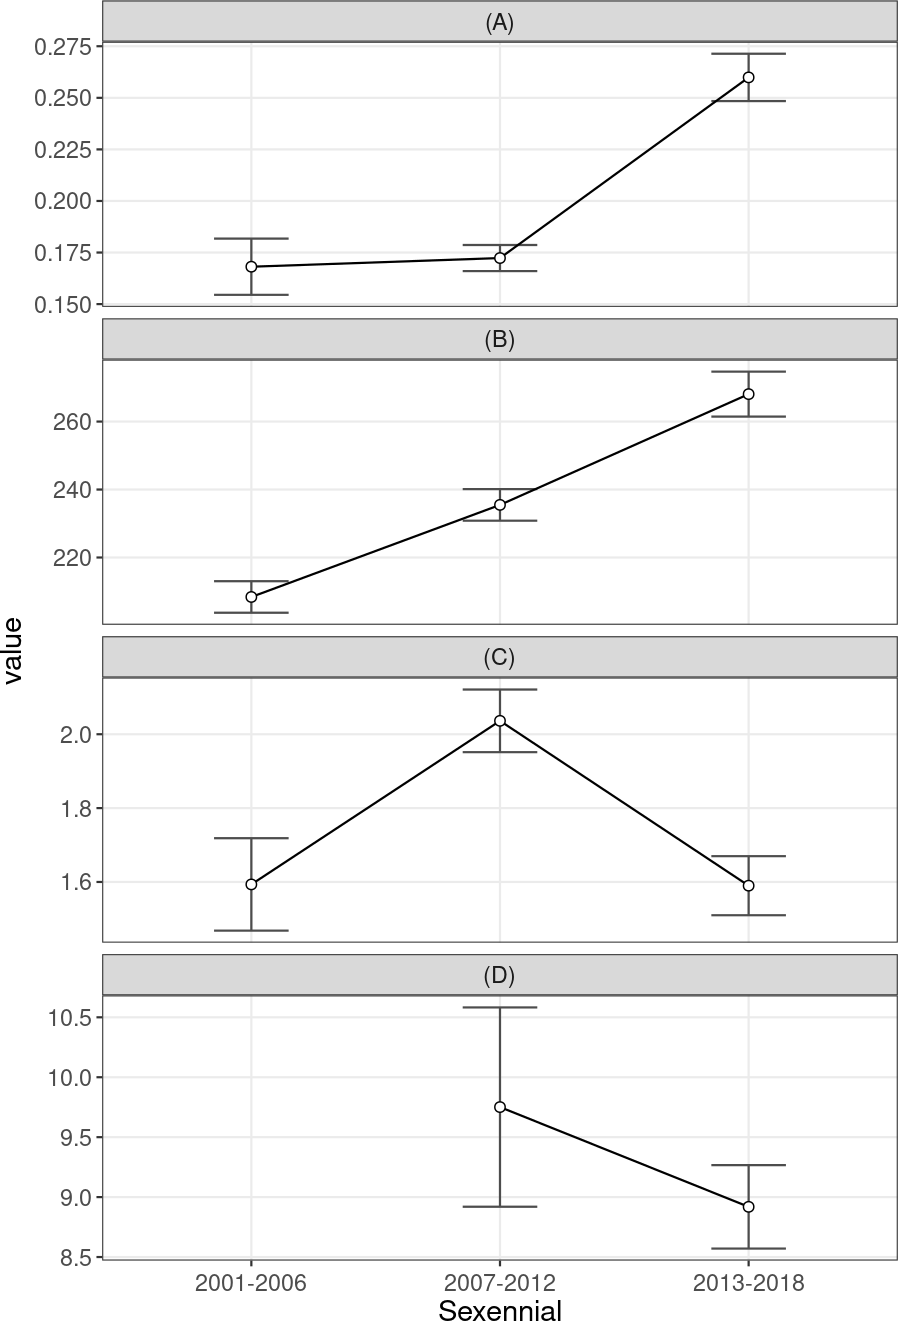
\includegraphics{img/modelling/aa-eda-ts-16} \end{center}

\begin{verbatim}
## $plot
\end{verbatim}

\begin{center}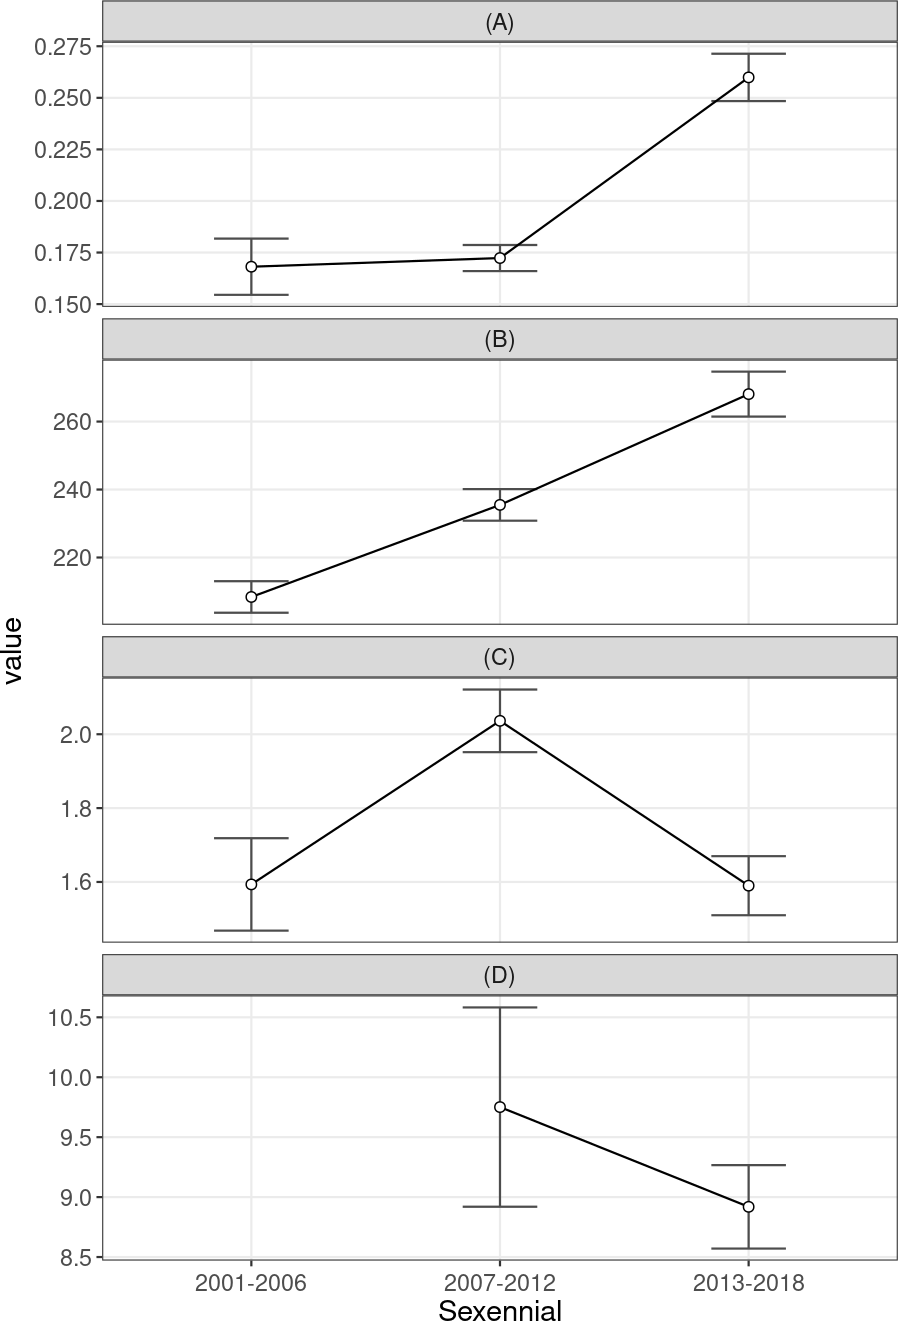
\includegraphics{img/modelling/aa-eda-ts-17} \end{center}

\begin{verbatim}
## 
## [[2]]
## 
## \begin{tabular}{l|l|l|l|l}
## \hline
## sexennial\_interval & Avg. area of forest loss in sq. km per 100 sq. km & Avg. number of forest loss patches \$<\$1 Ha per 100 sq. km & Avg. number of MODIS M6 fire points per 100 sq. km & Avg. number of VIRS V1 fire points per 100 sq. km\\
## \hline
## 2001-2006 & 0.17 (0.01) & 208.39 (4.64) & 1.59 (0.13) & -\\
## \hline
## 2007-2012 & 0.17 (0.01) & 235.48 (4.65) & 2.04 (0.08) & 9.75 (0.83)\\
## \hline
## 2013-2018 & 0.26 (0.01) & 268.08 (6.61) & 1.59 (0.08) & 8.92 (0.35)\\
## \hline
## \end{tabular}
## 
## $summaries_print_df
## # A tibble: 3 x 5
##   sexennial_interval `Avg. area of fore~ `Avg. number of for~ `Avg. number of M~
##   <fct>              <chr>               <chr>                <chr>             
## 1 2001-2006          0.17 (0.01)         208.39 (4.64)        1.59 (0.13)       
## 2 2007-2012          0.17 (0.01)         235.48 (4.65)        2.04 (0.08)       
## 3 2013-2018          0.26 (0.01)         268.08 (6.61)        1.59 (0.08)       
## # ... with 1 more variable:
## #   Avg. number of VIRS V1 fire points per 100 sq. km <chr>
## Decennials
periodic_summaries(
  source_table = four_variables_for_plots, measurevar = 'value',
  bins = 'decennial_interval', sum_variable = 'variable2', aspect_ratio = 1/3,
  smooth_span = 0.7, labels_angle = 0, xlab = 'Decennial', smooth = F, save = F,
  plot_filename = 'forest_loss_fire_points_line_plots_error_bars_2001_2018_four_variables_decennial.jpg',
  new_dev = F
)
\end{verbatim}

\begin{center}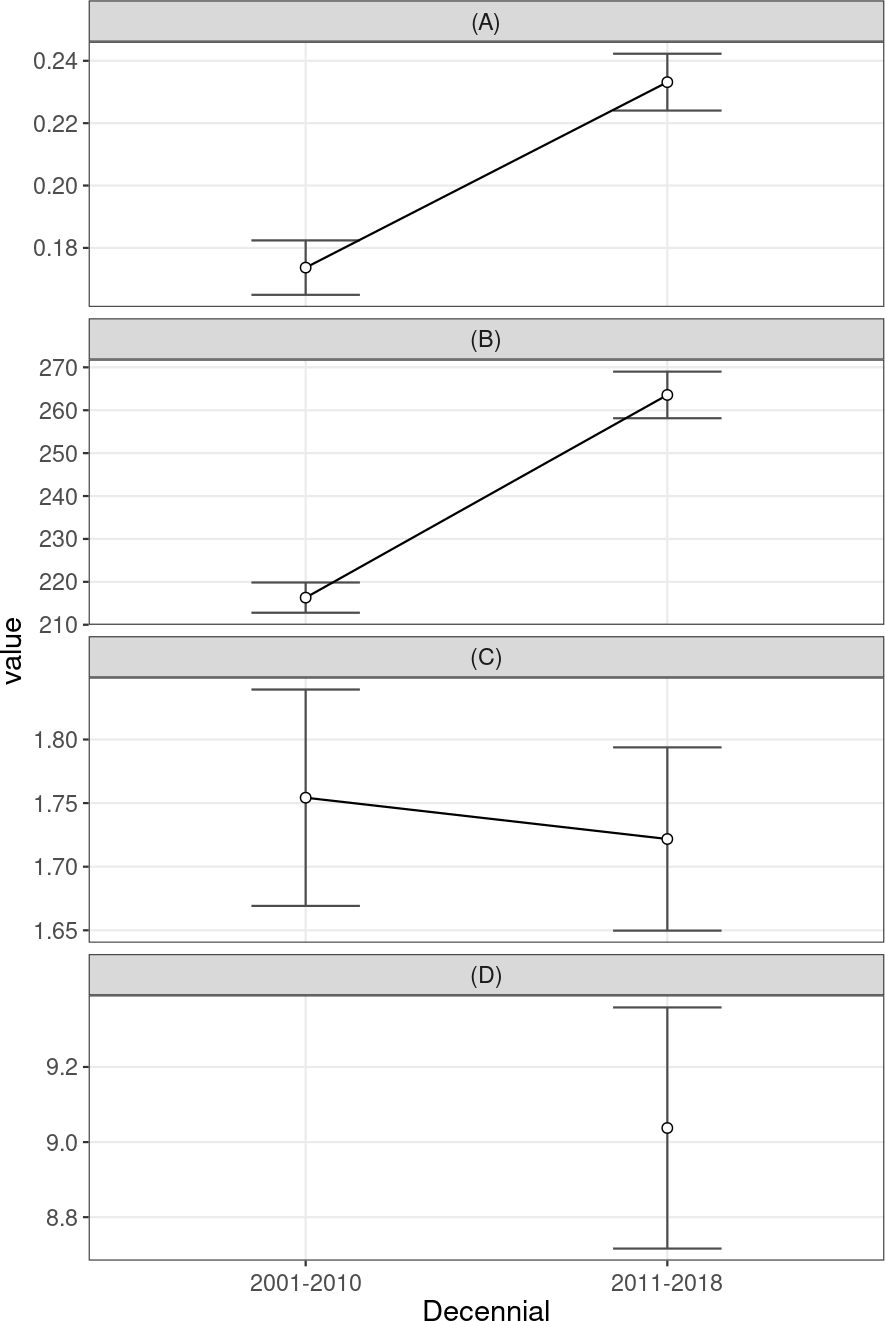
\includegraphics{img/modelling/aa-eda-ts-18} \end{center}

\begin{verbatim}
## $plot
\end{verbatim}

\begin{center}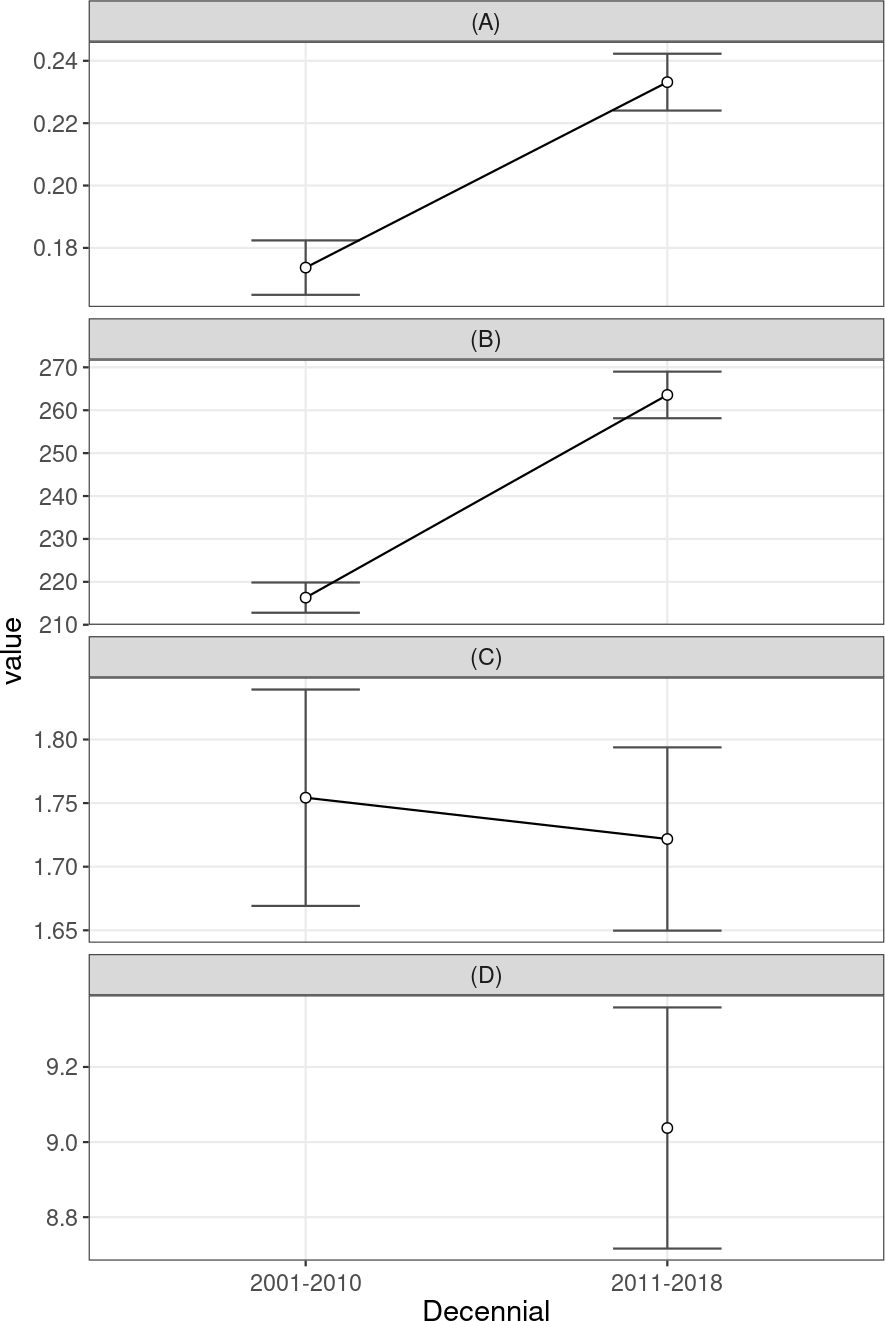
\includegraphics{img/modelling/aa-eda-ts-19} \end{center}

\begin{verbatim}
## 
## [[2]]
## 
## \begin{tabular}{l|l|l|l|l}
## \hline
## decennial\_interval & Avg. area of forest loss in sq. km per 100 sq. km & Avg. number of forest loss patches \$<\$1 Ha per 100 sq. km & Avg. number of MODIS M6 fire points per 100 sq. km & Avg. number of VIRS V1 fire points per 100 sq. km\\
## \hline
## 2001-2010 & 0.17 (0.01) & 216.32 (3.52) & 1.75 (0.09) & -\\
## \hline
## 2011-2018 & 0.23 (0.01) & 263.56 (5.43) & 1.72 (0.07) & 9.04 (0.32)\\
## \hline
## \end{tabular}
## 
## $summaries_print_df
## # A tibble: 2 x 5
##   decennial_interval `Avg. area of fore~ `Avg. number of for~ `Avg. number of M~
##   <fct>              <chr>               <chr>                <chr>             
## 1 2001-2010          0.17 (0.01)         216.32 (3.52)        1.75 (0.09)       
## 2 2011-2018          0.23 (0.01)         263.56 (5.43)        1.72 (0.07)       
## # ... with 1 more variable:
## #   Avg. number of VIRS V1 fire points per 100 sq. km <chr>

# Commented plot, only forest loss and fires modis
four_variables_for_plots_commented <- hexzonalfm %>% 
  select(!matches('ENLACE|AREASQM')) %>%
  st_drop_geometry %>% 
  gather(variable, value) %>% 
  mutate(year = as.numeric(create_year_from_string(variable)) + 2000,
         variable2 = create_variable_name_from_string(variable)) %>% 
  mutate(value = value * 100) %>% 
  mutate(variable2 = case_when(
    variable2 == 'NFIRESM6PSQKM' ~ 'Number of MODIS M6 fire points per 100 sq. km',
    variable2 == 'NFIRESV1PSQKM' ~ 'Number of VIRS V1 fire points per 100 sq. km',
    variable2 == 'NCLUMPSSMALLER1HAPSQKM' ~ 'Number of forest loss patches <1 Ha per 100 sq. km',
    variable2 == 'LOSSGREATER1HA_PUA' ~ 'Area of forest loss in sq. km per 100 sq. km'
  ))
four_variables_sum_commented <- summarySE(
  four_variables_for_plots_commented %>%
  filter(grepl('MODIS|^Area of', variable2)),
  measurevar="value", groupvars=c('year', 'variable2'))
four_variables_plot_commented <- four_variables_for_plots_commented %>%
  filter(grepl('MODIS|^Area of', variable2)) %>% 
  ggplot + aes(x = year, y = value) +
  scale_x_continuous(breaks = 2001:2018) + 
  theme_bw() +
  theme(axis.text.x = element_text(angle = 90, vjust = 0.5), panel.grid.minor = element_blank(),
        text = element_text(size = 14), aspect.ratio = 1/3) +
  geom_errorbar(data = four_variables_sum_commented, aes(ymin = value - se, ymax = value + se), colour = "grey30", width = .3) +
  geom_line(data = four_variables_sum_commented) +
  geom_point(data = four_variables_sum_commented, aes(x = year, y = value), size=2, shape=21, fill="white") +
  facet_wrap(~ variable2, scales = 'free_y', ncol = 1)
four_variables_plot_commented + geom_smooth(method = 'loess', span = 0.5)
\end{verbatim}

\begin{center}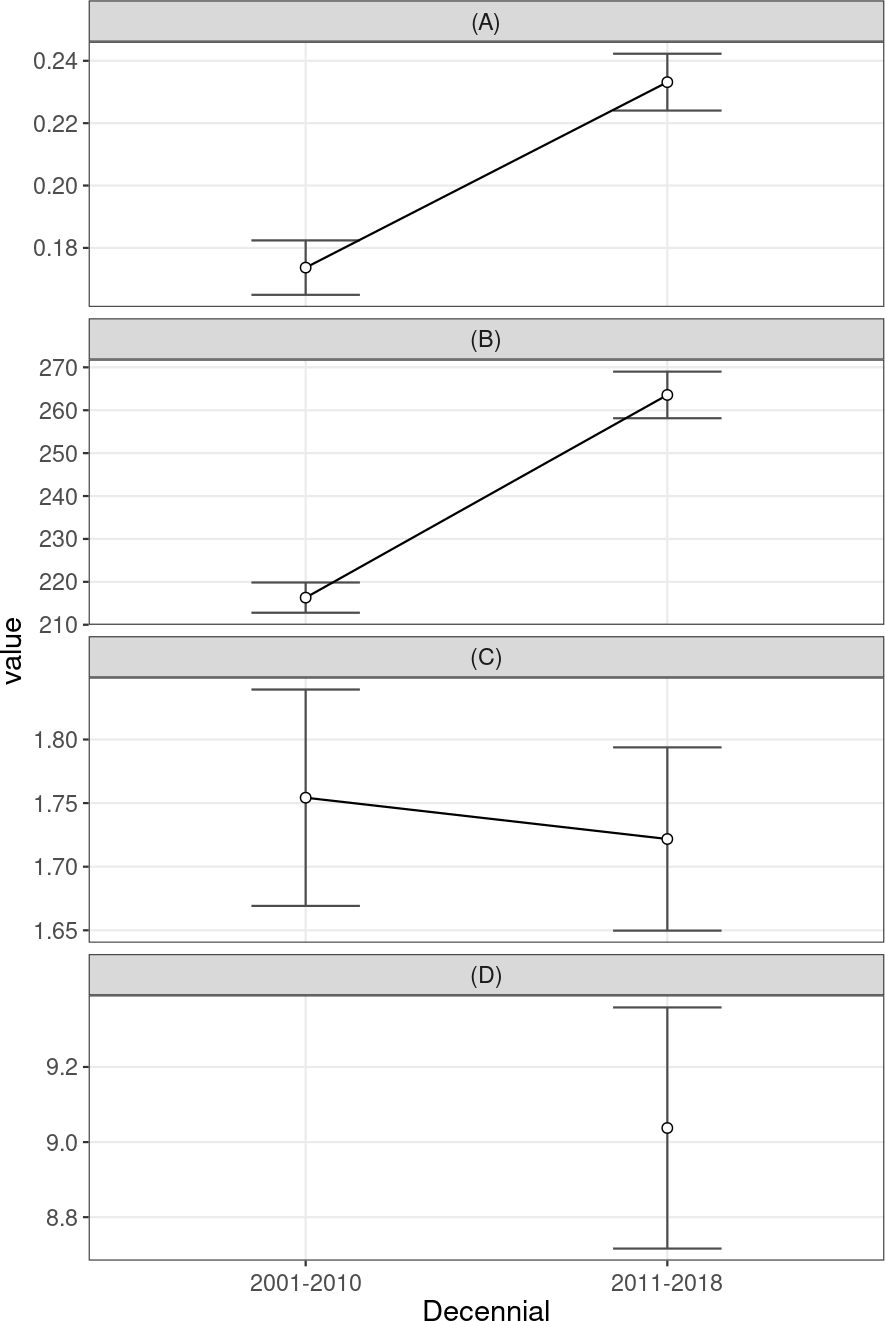
\includegraphics{img/modelling/aa-eda-ts-20} \end{center}

\begin{Shaded}
\begin{Highlighting}[]
\CommentTok{\# Fire (bottom chart) and forest{-}loss (top chart), were strongly associated during the first 15 years of the 21st Century in the Dominican Republic. However, in recent years, no such association exists. And yes, 2005, 2016 and 2017 were tough years}

\CommentTok{\# Time{-}series decomposition}
\NormalTok{four\_variables\_sum }\OtherTok{\textless{}{-}} \FunctionTok{summarySE}\NormalTok{(}
\NormalTok{  four\_variables\_for\_plots\_commented,}
  \AttributeTok{measurevar=}\StringTok{"value"}\NormalTok{, }\AttributeTok{groupvars=}\FunctionTok{c}\NormalTok{(}\StringTok{\textquotesingle{}year\textquotesingle{}}\NormalTok{, }\StringTok{\textquotesingle{}variable2\textquotesingle{}}\NormalTok{)) }\SpecialCharTok{\%\textgreater{}\%} 
   \FunctionTok{mutate}\NormalTok{(}\AttributeTok{variable2 =} \FunctionTok{case\_when}\NormalTok{(}
\NormalTok{    variable2 }\SpecialCharTok{==} \StringTok{\textquotesingle{}Number of MODIS M6 fire points per 100 sq. km\textquotesingle{}} \SpecialCharTok{\textasciitilde{}} \StringTok{\textquotesingle{}(C)\textquotesingle{}}\NormalTok{,}
\NormalTok{    variable2 }\SpecialCharTok{==} \StringTok{\textquotesingle{}Number of VIRS V1 fire points per 100 sq. km\textquotesingle{}} \SpecialCharTok{\textasciitilde{}} \StringTok{\textquotesingle{}(D)\textquotesingle{}}\NormalTok{,}
\NormalTok{    variable2 }\SpecialCharTok{==} \StringTok{\textquotesingle{}Number of forest loss patches \textless{}1 Ha per 100 sq. km\textquotesingle{}} \SpecialCharTok{\textasciitilde{}} \StringTok{\textquotesingle{}(B)\textquotesingle{}}\NormalTok{,}
\NormalTok{    variable2 }\SpecialCharTok{==} \StringTok{\textquotesingle{}Area of forest loss in sq. km per 100 sq. km\textquotesingle{}} \SpecialCharTok{\textasciitilde{}} \StringTok{\textquotesingle{}(A)\textquotesingle{}}
\NormalTok{  ))}
\NormalTok{four\_variables\_ts }\OtherTok{\textless{}{-}} \FunctionTok{sapply}\NormalTok{(}
  \FunctionTok{unique}\NormalTok{(four\_variables\_sum}\SpecialCharTok{$}\NormalTok{variable2),}
  \ControlFlowTok{function}\NormalTok{(x)}
    \FunctionTok{ts}\NormalTok{(}
\NormalTok{      four\_variables\_sum[four\_variables\_sum}\SpecialCharTok{$}\NormalTok{variable2 }\SpecialCharTok{==}\NormalTok{ x, }\StringTok{\textquotesingle{}value\textquotesingle{}}\NormalTok{],}
      \AttributeTok{start =} \ControlFlowTok{if}\NormalTok{(}\FunctionTok{grepl}\NormalTok{(}\StringTok{\textquotesingle{}D\textquotesingle{}}\NormalTok{, x)) }\DecValTok{2012} \ControlFlowTok{else} \DecValTok{2001}\NormalTok{, }\AttributeTok{frequency =} \DecValTok{1}\NormalTok{),}
  \AttributeTok{simplify =}\NormalTok{ F, }\AttributeTok{USE.NAMES =}\NormalTok{ T}
\NormalTok{  )}
\NormalTok{four\_variables\_ts\_filt }\OtherTok{\textless{}{-}} \FunctionTok{sapply}\NormalTok{(}
\NormalTok{  four\_variables\_ts,}
  \ControlFlowTok{function}\NormalTok{(x) }\FunctionTok{sapply}\NormalTok{(}\FunctionTok{c}\NormalTok{(}\StringTok{"HP"}\NormalTok{, }\StringTok{"CF"}\NormalTok{), }\ControlFlowTok{function}\NormalTok{(y) }\FunctionTok{mFilter}\NormalTok{(x, }\AttributeTok{filter =}\NormalTok{ y)),}
  \AttributeTok{simplify =}\NormalTok{ F, }\AttributeTok{USE.NAMES =}\NormalTok{ T}
\NormalTok{)}
\NormalTok{four\_variables\_ts\_filt\_for\_gg }\OtherTok{\textless{}{-}} \FunctionTok{lapply}\NormalTok{(}
\NormalTok{  four\_variables\_ts\_filt, }\ControlFlowTok{function}\NormalTok{(x) }\FunctionTok{ldply}\NormalTok{(}\FunctionTok{lapply}\NormalTok{(x, crear\_tabla\_de\_mfilter\_para\_gg), }\AttributeTok{.id =} \ConstantTok{NULL}\NormalTok{)) }\SpecialCharTok{\%\textgreater{}\%}
\NormalTok{  plyr}\SpecialCharTok{::}\FunctionTok{ldply}\NormalTok{(}\AttributeTok{.id =} \StringTok{\textquotesingle{}Variable\textquotesingle{}}\NormalTok{)}
\NormalTok{four\_variables\_ts\_filt\_gg }\OtherTok{\textless{}{-}}\NormalTok{ four\_variables\_ts\_filt\_for\_gg }\SpecialCharTok{\%\textgreater{}\%}
  \FunctionTok{gather}\NormalTok{(Component, Value, }\SpecialCharTok{{-}}\NormalTok{Variable, }\SpecialCharTok{{-}}\NormalTok{Year, }\SpecialCharTok{{-}}\NormalTok{Filter) }\SpecialCharTok{\%\textgreater{}\%} 
  \FunctionTok{mutate}\NormalTok{(}\AttributeTok{Variable =} \FunctionTok{gsub}\NormalTok{(}\StringTok{\textquotesingle{} per\textquotesingle{}}\NormalTok{, }\StringTok{\textquotesingle{}}\SpecialCharTok{\textbackslash{}n}\StringTok{per\textquotesingle{}}\NormalTok{, Variable)) }\SpecialCharTok{\%\textgreater{}\%} 
\NormalTok{  ggplot }\SpecialCharTok{+}
  \FunctionTok{aes}\NormalTok{(}\AttributeTok{x =}\NormalTok{ Year, }\AttributeTok{y =}\NormalTok{ Value, }\AttributeTok{color =}\NormalTok{ Component) }\SpecialCharTok{+}
    \FunctionTok{scale\_x\_continuous}\NormalTok{(}\AttributeTok{breaks =} \DecValTok{2001}\SpecialCharTok{:}\DecValTok{2018}\NormalTok{) }\SpecialCharTok{+} 
  \FunctionTok{theme\_bw}\NormalTok{() }\SpecialCharTok{+}
  \FunctionTok{theme}\NormalTok{(}\AttributeTok{axis.text.x =} \FunctionTok{element\_text}\NormalTok{(}\AttributeTok{angle =} \DecValTok{90}\NormalTok{, }\AttributeTok{vjust =} \FloatTok{0.5}\NormalTok{), }\AttributeTok{text =} \FunctionTok{element\_text}\NormalTok{(}\AttributeTok{size =} \DecValTok{14}\NormalTok{), }\AttributeTok{aspect.ratio =} \DecValTok{1}\SpecialCharTok{/}\DecValTok{2}\NormalTok{) }\SpecialCharTok{+}
  \FunctionTok{geom\_line}\NormalTok{() }\SpecialCharTok{+}
  \FunctionTok{facet\_grid}\NormalTok{(Variable }\SpecialCharTok{\textasciitilde{}}\NormalTok{ Filter, }\AttributeTok{scales =} \StringTok{\textquotesingle{}free\_y\textquotesingle{}}\NormalTok{)}
\NormalTok{four\_variables\_ts\_filt\_gg}
\end{Highlighting}
\end{Shaded}

\begin{center}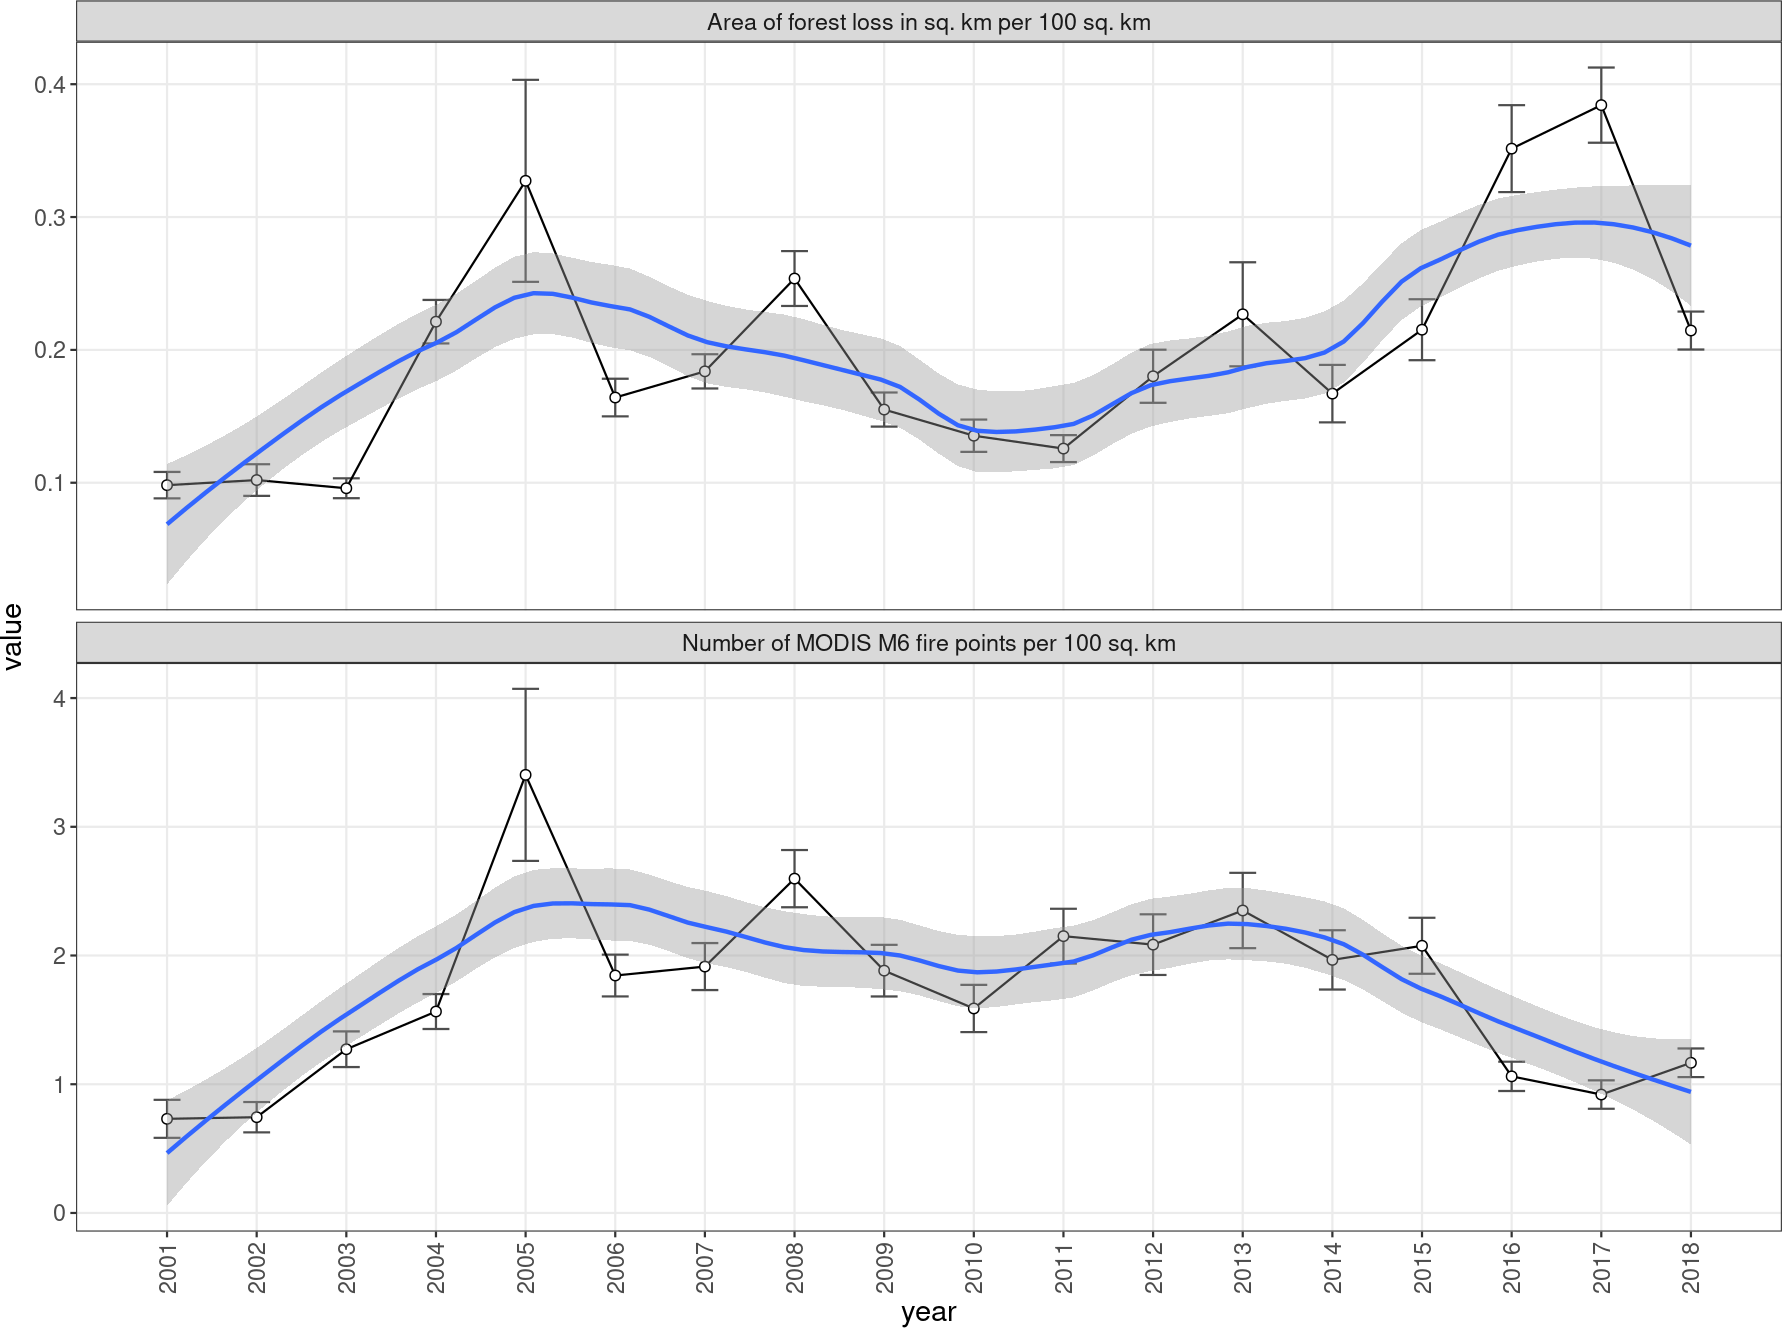
\includegraphics{img/modelling/aa-eda-ts-21} \end{center}

\begin{Shaded}
\begin{Highlighting}[]
\CommentTok{\# jpeg(\textquotesingle{}out/forest\_loss\_fire\_points\_line\_plots\_2001\_2018\_ts\_decomposition.jpg\textquotesingle{}, width = 2600, height = 2160, res = 250)}
\CommentTok{\# four\_variables\_ts\_filt\_gg}
\CommentTok{\# dev.off()}
\end{Highlighting}
\end{Shaded}

\hypertarget{yearly-forest-loss-and-fire-incidence-maps}{%
\subsection{Yearly forest-loss and fire incidence
maps}\label{yearly-forest-loss-and-fire-incidence-maps}}

\begin{Shaded}
\begin{Highlighting}[]
\NormalTok{hexzonalfm\_yearly\_maps }\OtherTok{\textless{}{-}}\NormalTok{ hexzonalfm }\SpecialCharTok{\%\textgreater{}\%}
    \FunctionTok{select}\NormalTok{(}\SpecialCharTok{!}\FunctionTok{matches}\NormalTok{(}\StringTok{"ENLACE|AREASQM"}\NormalTok{)) }\SpecialCharTok{\%\textgreater{}\%}
    \FunctionTok{gather}\NormalTok{(variable, value, }\SpecialCharTok{{-}}\NormalTok{geometry) }\SpecialCharTok{\%\textgreater{}\%}
    \FunctionTok{mutate}\NormalTok{(}\AttributeTok{year =} \FunctionTok{as.numeric}\NormalTok{(}\FunctionTok{create\_year\_from\_string}\NormalTok{(variable)) }\SpecialCharTok{+} \DecValTok{2000}\NormalTok{, }\AttributeTok{variable2 =} \FunctionTok{create\_variable\_name\_from\_string}\NormalTok{(variable)) }\SpecialCharTok{\%\textgreater{}\%}
    \FunctionTok{replace}\NormalTok{(}\FunctionTok{is.na}\NormalTok{(.), }\DecValTok{0}\NormalTok{) }\SpecialCharTok{\%\textgreater{}\%}
    \FunctionTok{mutate}\NormalTok{(}\AttributeTok{value =}\NormalTok{ value }\SpecialCharTok{*} \DecValTok{100}\NormalTok{) }\SpecialCharTok{\%\textgreater{}\%}
    \FunctionTok{mutate}\NormalTok{(}\AttributeTok{variable2 =} \FunctionTok{case\_when}\NormalTok{(variable2 }\SpecialCharTok{==} \StringTok{"NFIRESM6PSQKM"} \SpecialCharTok{\textasciitilde{}} \StringTok{"MODIS M6 fire points per 100 sq. km"}\NormalTok{,}
\NormalTok{        variable2 }\SpecialCharTok{==} \StringTok{"NFIRESV1PSQKM"} \SpecialCharTok{\textasciitilde{}} \StringTok{"VIRS V1 fire points per 100 sq. km"}\NormalTok{, variable2 }\SpecialCharTok{==}
            \StringTok{"NCLUMPSSMALLER1HAPSQKM"} \SpecialCharTok{\textasciitilde{}} \StringTok{"Forest loss patches \textless{}1 Ha per 100 sq. km"}\NormalTok{,}
\NormalTok{        variable2 }\SpecialCharTok{==} \StringTok{"LOSSGREATER1HA\_PUA"} \SpecialCharTok{\textasciitilde{}} \StringTok{"Forest loss in sq. km per 100 sq. km"}\NormalTok{)) }\SpecialCharTok{\%\textgreater{}\%}
    \FunctionTok{select}\NormalTok{(}\SpecialCharTok{{-}}\NormalTok{variable, }\AttributeTok{variable =}\NormalTok{ variable2)}
\FunctionTok{invisible}\NormalTok{(}\FunctionTok{map}\NormalTok{(hexzonalfm\_yearly\_maps}\SpecialCharTok{$}\NormalTok{variable }\SpecialCharTok{\%\textgreater{}\%}
\NormalTok{    unique, }\ControlFlowTok{function}\NormalTok{(x) \{}
\NormalTok{    m }\OtherTok{\textless{}{-}}\NormalTok{ hexzonalfm\_yearly\_maps }\SpecialCharTok{\%\textgreater{}\%}
        \FunctionTok{filter}\NormalTok{(variable }\SpecialCharTok{==}\NormalTok{ x) }\SpecialCharTok{\%\textgreater{}\%}
        \FunctionTok{tm\_shape}\NormalTok{() }\SpecialCharTok{+}\NormalTok{ \{}
        \ControlFlowTok{if}\NormalTok{ (}\FunctionTok{grepl}\NormalTok{(}\StringTok{"Forest loss in sq. km per 100 sq. km"}\NormalTok{, x)) }\FunctionTok{tm\_fill}\NormalTok{(}\AttributeTok{col =} \StringTok{"value"}\NormalTok{,}
            \AttributeTok{palette =} \FunctionTok{c}\NormalTok{(}\StringTok{"\#c9eebd"}\NormalTok{, }\StringTok{"\#69d6bd"}\NormalTok{, }\StringTok{"\#00bdc1"}\NormalTok{, }\StringTok{"\#10858d"}\NormalTok{), }\AttributeTok{size =} \FloatTok{0.1}\NormalTok{,}
            \AttributeTok{style =} \StringTok{"fixed"}\NormalTok{, }\AttributeTok{breaks =} \FunctionTok{c}\NormalTok{(}\DecValTok{0}\NormalTok{, }\FloatTok{0.2}\NormalTok{, }\FloatTok{0.4}\NormalTok{, }\DecValTok{1}\NormalTok{, }\DecValTok{7}\NormalTok{, }\FloatTok{13.5}\NormalTok{), }\AttributeTok{legend.is.portrait =}\NormalTok{ F,}
            \AttributeTok{legend.format =} \FunctionTok{list}\NormalTok{(}\AttributeTok{digits =} \DecValTok{2}\NormalTok{, }\AttributeTok{text.separator =} \StringTok{"{-}"}\NormalTok{, }\AttributeTok{scientific =} \ConstantTok{TRUE}\NormalTok{,}
                \AttributeTok{format =} \StringTok{"f"}\NormalTok{), }\AttributeTok{n =} \DecValTok{4}\NormalTok{) }\ControlFlowTok{else} \FunctionTok{tm\_fill}\NormalTok{(}\AttributeTok{col =} \StringTok{"value"}\NormalTok{, }\AttributeTok{palette =} \FunctionTok{c}\NormalTok{(}\StringTok{"\#c9eebd"}\NormalTok{,}
            \StringTok{"\#69d6bd"}\NormalTok{, }\StringTok{"\#00bdc1"}\NormalTok{, }\StringTok{"\#10858d"}\NormalTok{), }\AttributeTok{size =} \FloatTok{0.1}\NormalTok{, }\AttributeTok{style =} \StringTok{"kmeans"}\NormalTok{, }\AttributeTok{legend.is.portrait =}\NormalTok{ F,}
            \AttributeTok{legend.format =} \FunctionTok{list}\NormalTok{(}\AttributeTok{digits =} \DecValTok{2}\NormalTok{, }\AttributeTok{text.separator =} \StringTok{"{-}"}\NormalTok{, }\AttributeTok{scientific =} \ConstantTok{TRUE}\NormalTok{,}
                \AttributeTok{format =} \StringTok{"f"}\NormalTok{), }\AttributeTok{n =} \DecValTok{4}\NormalTok{)}
\NormalTok{    \} }\SpecialCharTok{+} \FunctionTok{tm\_borders}\NormalTok{(}\AttributeTok{col =} \StringTok{"grey15"}\NormalTok{, }\AttributeTok{lwd =} \FloatTok{0.3}\NormalTok{) }\SpecialCharTok{+} \FunctionTok{tm\_facets}\NormalTok{(}\AttributeTok{by =} \StringTok{"year"}\NormalTok{, }\AttributeTok{nrow =} \FunctionTok{ifelse}\NormalTok{(}\FunctionTok{grepl}\NormalTok{(}\StringTok{"VIRS"}\NormalTok{,}
\NormalTok{        x), }\DecValTok{2}\NormalTok{, }\DecValTok{3}\NormalTok{), }\AttributeTok{free.coords =} \ConstantTok{FALSE}\NormalTok{, }\AttributeTok{free.scales =} \ConstantTok{FALSE}\NormalTok{) }\SpecialCharTok{+} \FunctionTok{tm\_layout}\NormalTok{(}\AttributeTok{panel.label.size =} \FloatTok{1.75}\NormalTok{,}
        \AttributeTok{legend.title.size =} \FloatTok{1e{-}05}\NormalTok{, }\AttributeTok{legend.text.size =} \DecValTok{3}\NormalTok{, }\AttributeTok{legend.outside.position =} \StringTok{"bottom"}\NormalTok{,}
        \AttributeTok{legend.outside.size =} \FloatTok{0.1}\NormalTok{, }\AttributeTok{outer.margins =} \FunctionTok{c}\NormalTok{(}\SpecialCharTok{{-}}\FloatTok{0.02}\NormalTok{, }\FloatTok{0.01}\NormalTok{, }\SpecialCharTok{{-}}\FloatTok{0.02}\NormalTok{, }\FloatTok{0.01}\NormalTok{), }\AttributeTok{inner.margins =} \DecValTok{0}\NormalTok{) }\SpecialCharTok{+}
        \FunctionTok{tm\_shape}\NormalTok{(seaocean) }\SpecialCharTok{+} \FunctionTok{tm\_borders}\NormalTok{() }\SpecialCharTok{+} \FunctionTok{tm\_fill}\NormalTok{(}\AttributeTok{col =} \StringTok{"white"}\NormalTok{)  }\CommentTok{\#+ }
    \CommentTok{\# tm\_shape(points\_of\_interest) + tm\_text(\textquotesingle{}code\textquotesingle{}, size = 2, col = \textquotesingle{}black\textquotesingle{},}
    \CommentTok{\# fontface = \textquotesingle{}bold\textquotesingle{}, bg.color = \textquotesingle{}white\textquotesingle{}, bg.alpha = 0.5)}
\NormalTok{    n }\OtherTok{\textless{}{-}} \FunctionTok{paste0}\NormalTok{(}\StringTok{"out/yearly\_"}\NormalTok{, x }\SpecialCharTok{\%\textgreater{}\%}
        \FunctionTok{gsub}\NormalTok{(}\StringTok{" |\textless{}|}\SpecialCharTok{\textbackslash{}\textbackslash{}}\StringTok{."}\NormalTok{, }\StringTok{"\_"}\NormalTok{, .) }\SpecialCharTok{\%\textgreater{}\%}
        \FunctionTok{gsub}\NormalTok{(}\StringTok{"\_\_"}\NormalTok{, }\StringTok{"\_"}\NormalTok{, .) }\SpecialCharTok{\%\textgreater{}\%}
\NormalTok{        tolower, }\StringTok{".jpg"}\NormalTok{)}
    \CommentTok{\# jpeg(n, width = 3840, height = 1700, res = 300) dev.new()}
    \FunctionTok{print}\NormalTok{(m)}
    \CommentTok{\# dev.off()}
\NormalTok{\}))}
\end{Highlighting}
\end{Shaded}

\begin{center}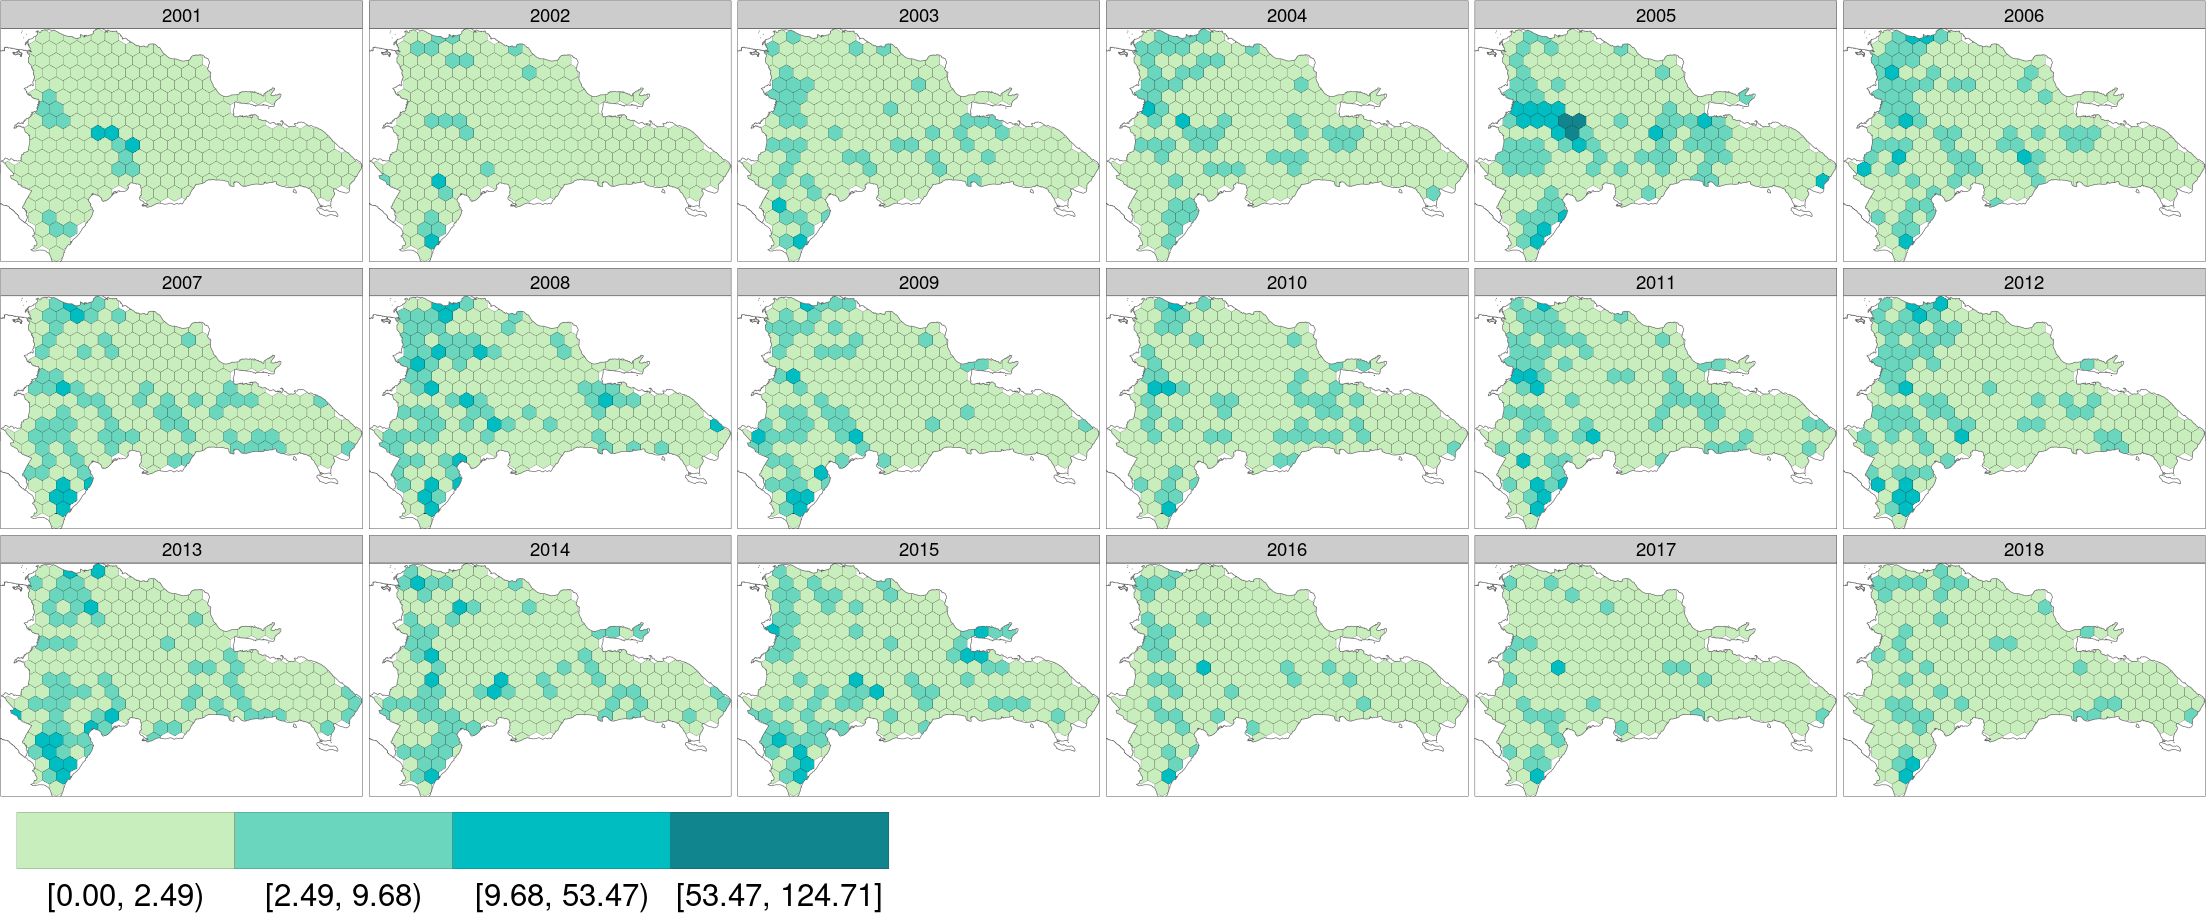
\includegraphics{img/modelling/aa-yearly-forest-loss-maps-1} \end{center}

\begin{center}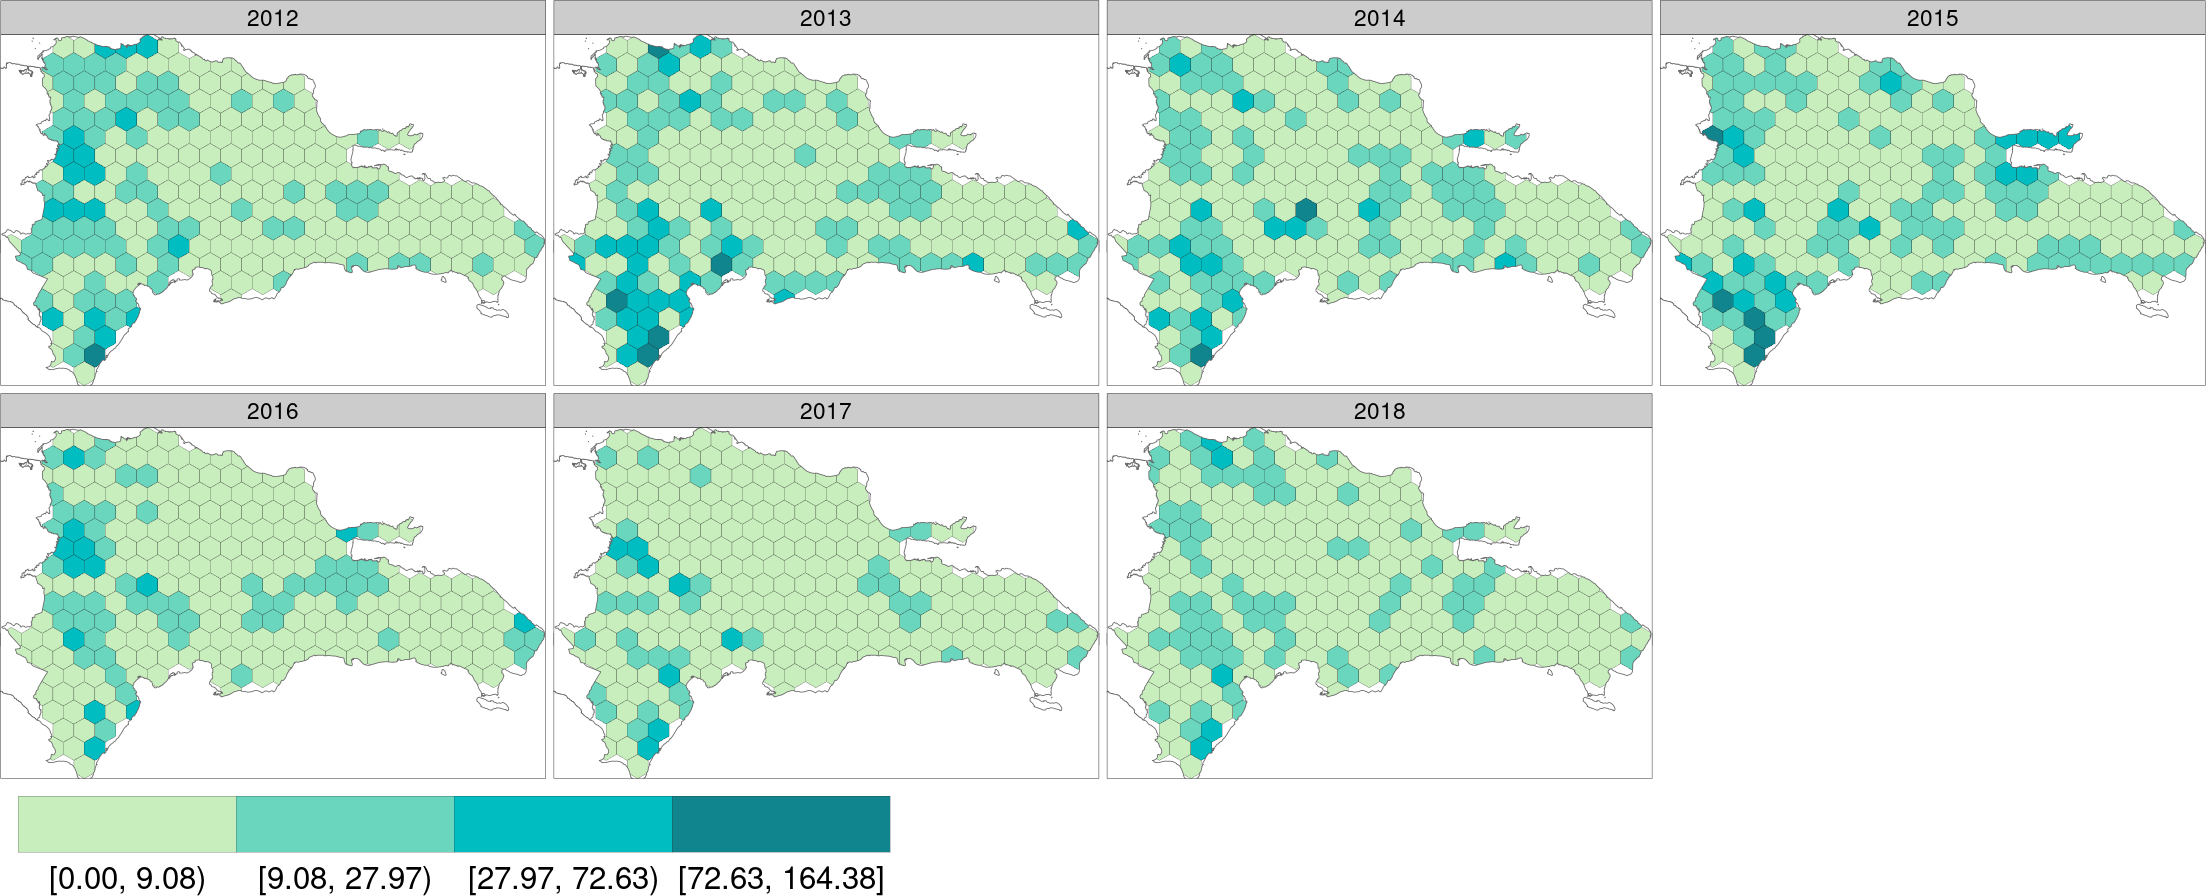
\includegraphics{img/modelling/aa-yearly-forest-loss-maps-2} \end{center}

\begin{center}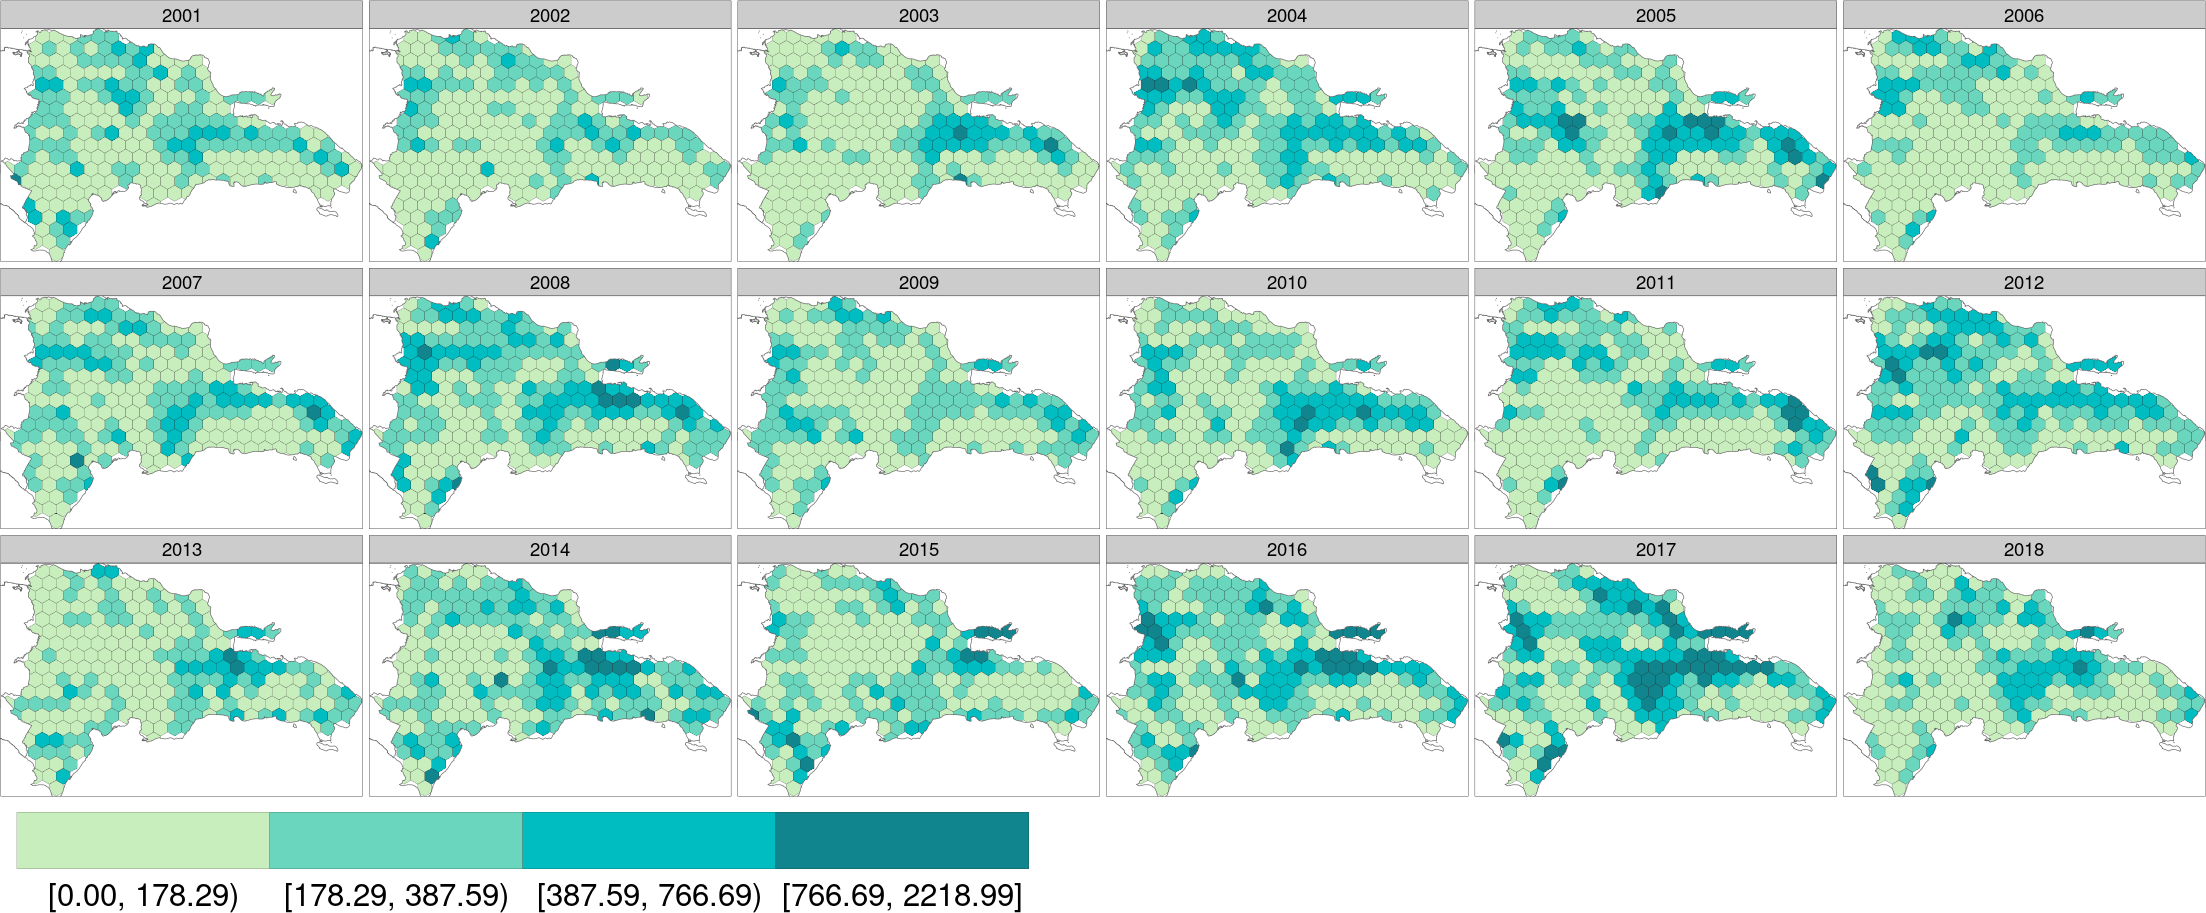
\includegraphics{img/modelling/aa-yearly-forest-loss-maps-3} \end{center}

\begin{center}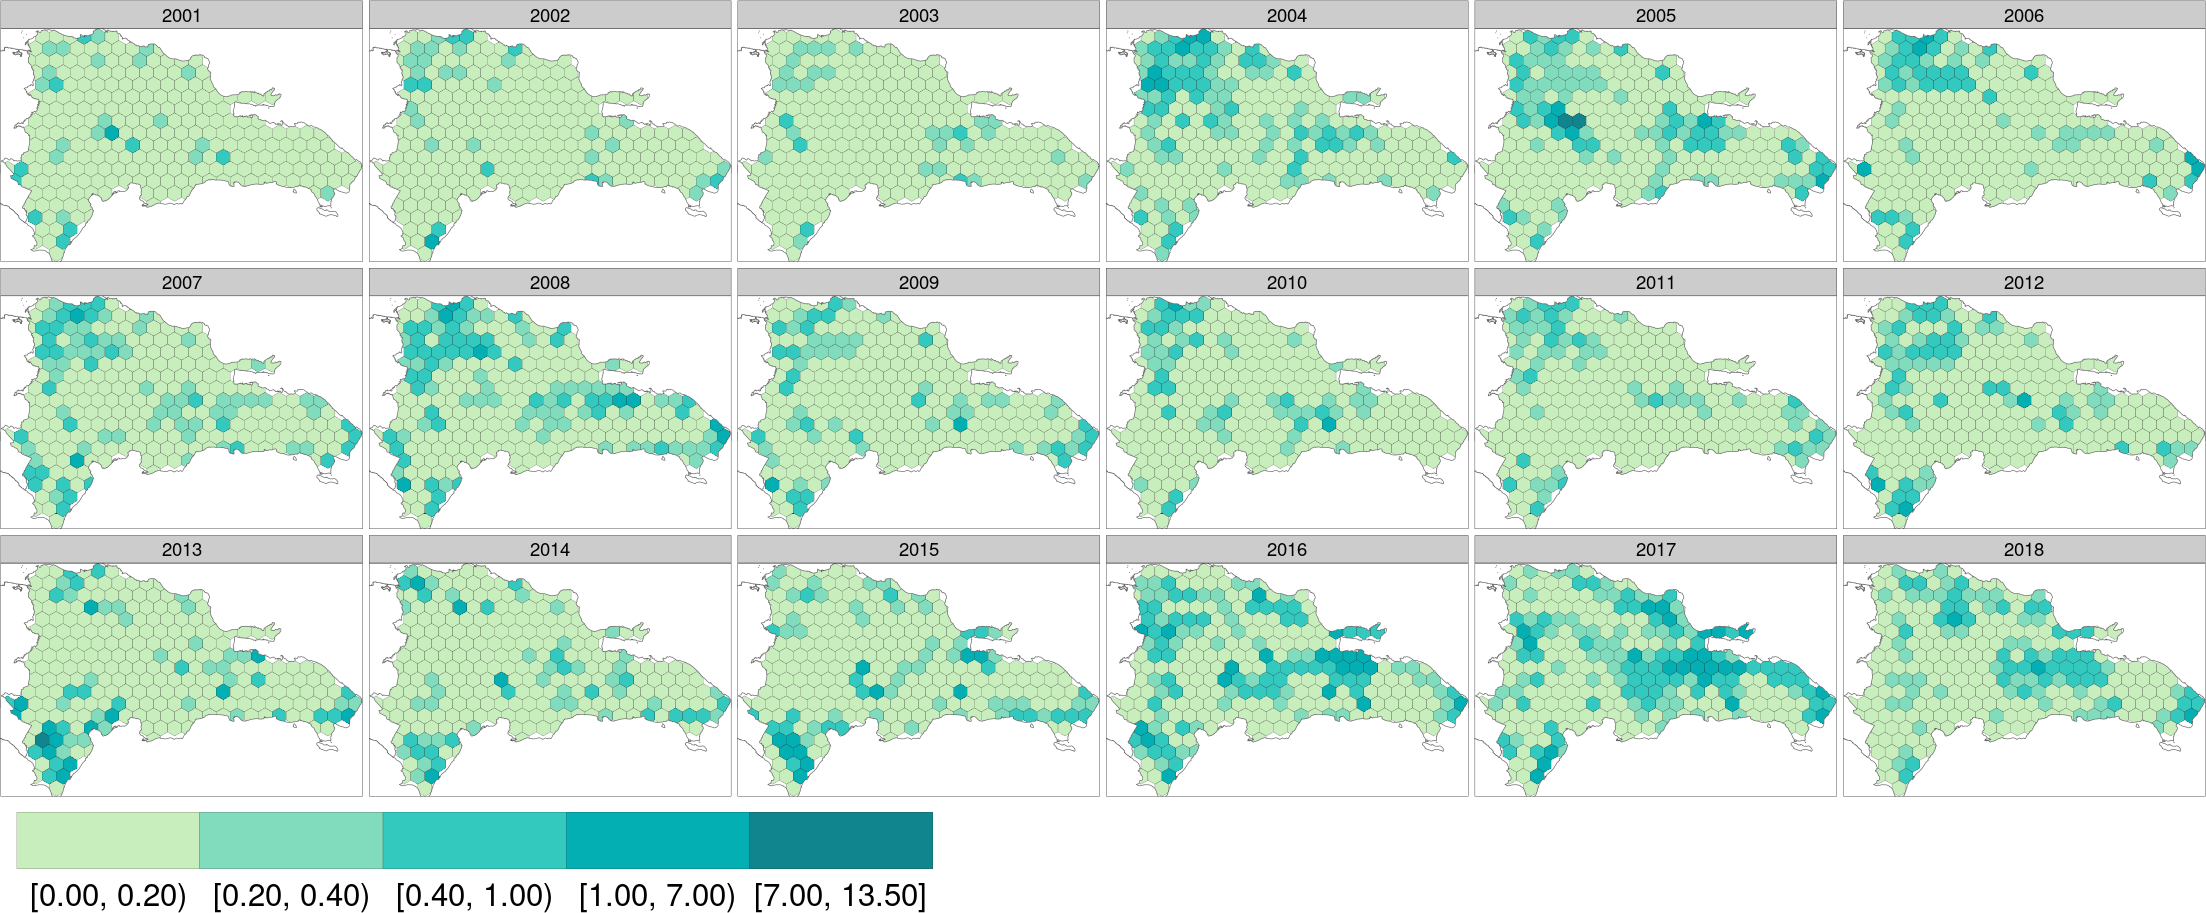
\includegraphics{img/modelling/aa-yearly-forest-loss-maps-4} \end{center}

\hypertarget{transformations}{%
\subsection{Transformations}\label{transformations}}

\begin{Shaded}
\begin{Highlighting}[]
\CommentTok{\# * Transformations using Tukey\textquotesingle{}s Ladder of Powers}
\NormalTok{hexzonalfmt }\OtherTok{\textless{}{-}}\NormalTok{ hexzonalfm }\SpecialCharTok{\%\textgreater{}\%}
  \FunctionTok{mutate}\NormalTok{(}\FunctionTok{across}\NormalTok{(}\SpecialCharTok{!}\FunctionTok{matches}\NormalTok{(}\StringTok{\textquotesingle{}ENLACE|AREASQM|geometry\textquotesingle{}}\NormalTok{),}
                \FunctionTok{list}\NormalTok{(}\StringTok{\textquotesingle{}TLP\textquotesingle{}} \OtherTok{=} \ErrorTok{\textasciitilde{}} \FunctionTok{transformTukey}\NormalTok{(.x, }\AttributeTok{plotit =}\NormalTok{ F, }\AttributeTok{quiet =}\NormalTok{ T),}
                \StringTok{\textquotesingle{}LAMBDA\textquotesingle{}} \OtherTok{=} \ErrorTok{\textasciitilde{}} \FunctionTok{transformTukey}\NormalTok{(}\AttributeTok{x =}\NormalTok{ .x, }\AttributeTok{plotit =}\NormalTok{ F, }\AttributeTok{returnLambda =}\NormalTok{ T, }\AttributeTok{quiet =}\NormalTok{ T)[[}\StringTok{\textquotesingle{}lambda\textquotesingle{}}\NormalTok{]]))) }\SpecialCharTok{\%\textgreater{}\%} 
  \FunctionTok{mutate}\NormalTok{(}\FunctionTok{across}\NormalTok{(}\FunctionTok{matches}\NormalTok{(}\StringTok{\textquotesingle{}TLP$\textquotesingle{}}\NormalTok{),}
                 \FunctionTok{list}\NormalTok{(}\StringTok{\textquotesingle{}SWPVAL\textquotesingle{}} \OtherTok{=} \ErrorTok{\textasciitilde{}} \FunctionTok{shapiro.test}\NormalTok{(.x)}\SpecialCharTok{$}\NormalTok{p.value,}
                      \StringTok{\textquotesingle{}ADPVAL\textquotesingle{}} \OtherTok{=} \ErrorTok{\textasciitilde{}} \FunctionTok{ad.test}\NormalTok{(.x)}\SpecialCharTok{$}\NormalTok{p.value, }
                      \StringTok{\textquotesingle{}MTPVAL\textquotesingle{}} \OtherTok{=} \ErrorTok{\textasciitilde{}} \FunctionTok{moran.test}\NormalTok{(.x, }\AttributeTok{listw =}\NormalTok{ hexww, }\AttributeTok{na.action =}\NormalTok{ na.exclude, }\AttributeTok{zero.policy =}\NormalTok{ T)}\SpecialCharTok{$}\NormalTok{p.value,}
                      \StringTok{\textquotesingle{}MIEST\textquotesingle{}} \OtherTok{=} \ErrorTok{\textasciitilde{}} \FunctionTok{moran.test}\NormalTok{(.x, }\AttributeTok{listw =}\NormalTok{ hexww, }\AttributeTok{na.action =}\NormalTok{ na.exclude, }\AttributeTok{zero.policy =}\NormalTok{ T)}\SpecialCharTok{$}\NormalTok{estimate[[}\DecValTok{1}\NormalTok{]],}
                      \StringTok{\textquotesingle{}MIVAR\textquotesingle{}} \OtherTok{=} \ErrorTok{\textasciitilde{}} \FunctionTok{moran.test}\NormalTok{(.x, }\AttributeTok{listw =}\NormalTok{ hexww, }\AttributeTok{na.action =}\NormalTok{ na.exclude, }\AttributeTok{zero.policy =}\NormalTok{ T)}\SpecialCharTok{$}\NormalTok{estimate[[}\DecValTok{3}\NormalTok{]],}
                      \StringTok{\textquotesingle{}LENGTH\textquotesingle{}} \OtherTok{=} \ErrorTok{\textasciitilde{}} \FunctionTok{length}\NormalTok{(.x))))}
\NormalTok{lambda\_tests }\OtherTok{\textless{}{-}}\NormalTok{ hexzonalfmt }\SpecialCharTok{\%\textgreater{}\%}
\NormalTok{  st\_drop\_geometry }\SpecialCharTok{\%\textgreater{}\%}
  \FunctionTok{select}\NormalTok{(}\FunctionTok{matches}\NormalTok{(}\StringTok{\textquotesingle{}SWPVAL$|ADPVAL$|MTPVAL|MIEST|MIVAR|LENGTH\textquotesingle{}}\NormalTok{)) }\SpecialCharTok{\%\textgreater{}\%}
\NormalTok{  unique }\SpecialCharTok{\%\textgreater{}\%}
  \FunctionTok{gather}\NormalTok{(variable, value) }\SpecialCharTok{\%\textgreater{}\%} 
  \FunctionTok{separate}\NormalTok{(variable, }\AttributeTok{into =} \FunctionTok{c}\NormalTok{(}\StringTok{\textquotesingle{}variable\textquotesingle{}}\NormalTok{, }\StringTok{\textquotesingle{}test\textquotesingle{}}\NormalTok{), }\AttributeTok{sep =} \StringTok{\textquotesingle{}\_TLP\_\textquotesingle{}}\NormalTok{) }\SpecialCharTok{\%\textgreater{}\%}
  \FunctionTok{mutate}\NormalTok{(}\AttributeTok{variable =} \FunctionTok{paste0}\NormalTok{(variable, }\StringTok{\textquotesingle{}\_TLP\textquotesingle{}}\NormalTok{)) }\SpecialCharTok{\%\textgreater{}\%} 
  \FunctionTok{spread}\NormalTok{(}\AttributeTok{key =}\NormalTok{ test, }\AttributeTok{value =}\NormalTok{ value) }\SpecialCharTok{\%\textgreater{}\%} 
  \FunctionTok{mutate}\NormalTok{(}\AttributeTok{year =} \FunctionTok{as.numeric}\NormalTok{(}\FunctionTok{create\_year\_from\_string}\NormalTok{(variable))}\SpecialCharTok{+}\DecValTok{2000}\NormalTok{,}
         \AttributeTok{variable2 =} \FunctionTok{create\_variable\_name\_from\_string}\NormalTok{(variable))}
\NormalTok{lambda\_tests }\SpecialCharTok{\%\textgreater{}\%} \FunctionTok{arrange}\NormalTok{(SWPVAL)}
\DocumentationTok{\#\#                              variable       ADPVAL LENGTH     MIEST       MIVAR}
\DocumentationTok{\#\# 1            NFIRESM6\_YEAR1\_PSQKM\_TLP 3.700000e{-}24    253 0.2337788 0.001546848}
\DocumentationTok{\#\# 2            NFIRESM6\_YEAR2\_PSQKM\_TLP 3.700000e{-}24    253 0.3377643 0.001549263}
\DocumentationTok{\#\# 3           NFIRESM6\_YEAR17\_PSQKM\_TLP 3.700000e{-}24    253 0.2021339 0.001552937}
\DocumentationTok{\#\# 4           NFIRESM6\_YEAR16\_PSQKM\_TLP 3.700000e{-}24    253 0.2822651 0.001552164}
\DocumentationTok{\#\# 5            NFIRESM6\_YEAR3\_PSQKM\_TLP 3.700000e{-}24    253 0.2162494 0.001550242}
\DocumentationTok{\#\# 6           NFIRESM6\_YEAR18\_PSQKM\_TLP 3.700000e{-}24    253 0.2516554 0.001552536}
\DocumentationTok{\#\# 7           NFIRESM6\_YEAR10\_PSQKM\_TLP 3.700000e{-}24    253 0.2591194 0.001548620}
\DocumentationTok{\#\# 8           NFIRESM6\_YEAR12\_PSQKM\_TLP 3.700000e{-}24    253 0.3486194 0.001552495}
\DocumentationTok{\#\# 9            NFIRESM6\_YEAR7\_PSQKM\_TLP 3.700000e{-}24    253 0.3116846 0.001553405}
\DocumentationTok{\#\# 10          NFIRESM6\_YEAR13\_PSQKM\_TLP 3.700000e{-}24    253 0.3424536 0.001551612}
\DocumentationTok{\#\# 11           NFIRESM6\_YEAR5\_PSQKM\_TLP 3.700000e{-}24    253 0.3835136 0.001548710}
\DocumentationTok{\#\# 12          NFIRESM6\_YEAR14\_PSQKM\_TLP 8.219447e{-}23    253 0.2598008 0.001550306}
\DocumentationTok{\#\# 13          NFIRESM6\_YEAR11\_PSQKM\_TLP 5.658013e{-}23    253 0.3085412 0.001553839}
\DocumentationTok{\#\# 14           NFIRESM6\_YEAR4\_PSQKM\_TLP 1.345327e{-}22    253 0.3420576 0.001554705}
\DocumentationTok{\#\# 15           NFIRESM6\_YEAR6\_PSQKM\_TLP 2.644369e{-}21    253 0.3115173 0.001553679}
\DocumentationTok{\#\# 16          NFIRESM6\_YEAR15\_PSQKM\_TLP 3.254400e{-}20    253 0.2907386 0.001552204}
\DocumentationTok{\#\# 17           NFIRESM6\_YEAR9\_PSQKM\_TLP 2.576325e{-}20    253 0.3184660 0.001551763}
\DocumentationTok{\#\# 18       YEAR5\_LOSSGREATER1HA\_PUA\_TLP 7.452685e{-}10    253 0.3746342 0.001521956}
\DocumentationTok{\#\# 19           NFIRESM6\_YEAR8\_PSQKM\_TLP 5.271077e{-}13    253 0.2823828 0.001553801}
\DocumentationTok{\#\# 20      YEAR13\_LOSSGREATER1HA\_PUA\_TLP 3.071271e{-}09    253 0.4035400 0.001543450}
\DocumentationTok{\#\# 21          NFIRESV1\_YEAR17\_PSQKM\_TLP 3.154195e{-}07    253 0.2972833 0.001548334}
\DocumentationTok{\#\# 22       YEAR2\_LOSSGREATER1HA\_PUA\_TLP 1.684977e{-}05    253 0.3145905 0.001537406}
\DocumentationTok{\#\# 23          NFIRESV1\_YEAR16\_PSQKM\_TLP 3.519062e{-}05    253 0.3334186 0.001553566}
\DocumentationTok{\#\# 24      YEAR14\_LOSSGREATER1HA\_PUA\_TLP 1.742845e{-}05    253 0.2034278 0.001540054}
\DocumentationTok{\#\# 25          NFIRESV1\_YEAR14\_PSQKM\_TLP 7.589478e{-}05    253 0.1883641 0.001544140}
\DocumentationTok{\#\# 26          NFIRESV1\_YEAR13\_PSQKM\_TLP 3.930253e{-}05    253 0.3986340 0.001550418}
\DocumentationTok{\#\# 27       YEAR1\_LOSSGREATER1HA\_PUA\_TLP 4.468161e{-}05    253 0.1823457 0.001543320}
\DocumentationTok{\#\# 28      YEAR15\_LOSSGREATER1HA\_PUA\_TLP 7.199124e{-}06    253 0.3558061 0.001544521}
\DocumentationTok{\#\# 29      YEAR12\_LOSSGREATER1HA\_PUA\_TLP 3.652148e{-}05    253 0.2499134 0.001541624}
\DocumentationTok{\#\# 30          NFIRESV1\_YEAR15\_PSQKM\_TLP 3.120724e{-}04    253 0.3574704 0.001548291}
\DocumentationTok{\#\# 31          NFIRESV1\_YEAR12\_PSQKM\_TLP 5.516181e{-}04    253 0.3264984 0.001549331}
\DocumentationTok{\#\# 32       YEAR3\_LOSSGREATER1HA\_PUA\_TLP 2.024899e{-}03    253 0.2045038 0.001547191}
\DocumentationTok{\#\# 33       YEAR6\_LOSSGREATER1HA\_PUA\_TLP 1.135303e{-}03    253 0.4201354 0.001549351}
\DocumentationTok{\#\# 34      YEAR11\_LOSSGREATER1HA\_PUA\_TLP 3.310997e{-}03    253 0.4093635 0.001552594}
\DocumentationTok{\#\# 35          NFIRESV1\_YEAR18\_PSQKM\_TLP 1.942503e{-}02    253 0.3097203 0.001550336}
\DocumentationTok{\#\# 36       YEAR9\_LOSSGREATER1HA\_PUA\_TLP 8.395511e{-}03    253 0.3020721 0.001548113}
\DocumentationTok{\#\# 37      YEAR10\_LOSSGREATER1HA\_PUA\_TLP 1.533671e{-}02    253 0.3355577 0.001547599}
\DocumentationTok{\#\# 38      YEAR16\_LOSSGREATER1HA\_PUA\_TLP 3.135870e{-}02    253 0.3785848 0.001547795}
\DocumentationTok{\#\# 39 NCLUMPSSMALLER1HA\_YEAR15\_PSQKM\_TLP 3.025917e{-}02    253 0.4670470 0.001543966}
\DocumentationTok{\#\# 40       YEAR8\_LOSSGREATER1HA\_PUA\_TLP 3.598151e{-}02    253 0.3817155 0.001547634}
\DocumentationTok{\#\# 41      YEAR18\_LOSSGREATER1HA\_PUA\_TLP 1.137622e{-}01    253 0.4523400 0.001552081}
\DocumentationTok{\#\# 42       YEAR4\_LOSSGREATER1HA\_PUA\_TLP 1.666697e{-}01    253 0.4489153 0.001549675}
\DocumentationTok{\#\# 43       YEAR7\_LOSSGREATER1HA\_PUA\_TLP 4.817272e{-}02    253 0.3354710 0.001551609}
\DocumentationTok{\#\# 44  NCLUMPSSMALLER1HA\_YEAR6\_PSQKM\_TLP 1.597245e{-}01    253 0.5529876 0.001553275}
\DocumentationTok{\#\# 45  NCLUMPSSMALLER1HA\_YEAR5\_PSQKM\_TLP 3.202336e{-}02    253 0.5654756 0.001546217}
\DocumentationTok{\#\# 46      YEAR17\_LOSSGREATER1HA\_PUA\_TLP 3.857454e{-}01    253 0.4656550 0.001551202}
\DocumentationTok{\#\# 47 NCLUMPSSMALLER1HA\_YEAR16\_PSQKM\_TLP 6.648748e{-}02    253 0.5020020 0.001546628}
\DocumentationTok{\#\# 48 NCLUMPSSMALLER1HA\_YEAR17\_PSQKM\_TLP 7.455826e{-}01    253 0.5597302 0.001553129}
\DocumentationTok{\#\# 49 NCLUMPSSMALLER1HA\_YEAR18\_PSQKM\_TLP 6.480536e{-}01    253 0.5327632 0.001551403}
\DocumentationTok{\#\# 50  NCLUMPSSMALLER1HA\_YEAR2\_PSQKM\_TLP 6.783075e{-}01    253 0.4853745 0.001552623}
\DocumentationTok{\#\# 51 NCLUMPSSMALLER1HA\_YEAR14\_PSQKM\_TLP 5.108259e{-}01    253 0.4254865 0.001549887}
\DocumentationTok{\#\# 52  NCLUMPSSMALLER1HA\_YEAR9\_PSQKM\_TLP 4.712184e{-}01    253 0.4642466 0.001553335}
\DocumentationTok{\#\# 53  NCLUMPSSMALLER1HA\_YEAR8\_PSQKM\_TLP 7.387968e{-}01    253 0.5479653 0.001552470}
\DocumentationTok{\#\# 54 NCLUMPSSMALLER1HA\_YEAR13\_PSQKM\_TLP 3.552775e{-}01    253 0.4913922 0.001548249}
\DocumentationTok{\#\# 55  NCLUMPSSMALLER1HA\_YEAR7\_PSQKM\_TLP 5.218663e{-}01    253 0.4578194 0.001549336}
\DocumentationTok{\#\# 56  NCLUMPSSMALLER1HA\_YEAR4\_PSQKM\_TLP 4.095683e{-}01    253 0.5931522 0.001552440}
\DocumentationTok{\#\# 57 NCLUMPSSMALLER1HA\_YEAR12\_PSQKM\_TLP 8.930608e{-}01    253 0.4392756 0.001551148}
\DocumentationTok{\#\# 58  NCLUMPSSMALLER1HA\_YEAR3\_PSQKM\_TLP 5.789775e{-}01    253 0.5685404 0.001550321}
\DocumentationTok{\#\# 59 NCLUMPSSMALLER1HA\_YEAR11\_PSQKM\_TLP 8.312023e{-}01    253 0.6050384 0.001550152}
\DocumentationTok{\#\# 60  NCLUMPSSMALLER1HA\_YEAR1\_PSQKM\_TLP 9.154352e{-}01    253 0.3554933 0.001551502}
\DocumentationTok{\#\# 61 NCLUMPSSMALLER1HA\_YEAR10\_PSQKM\_TLP 9.049471e{-}01    253 0.5461478 0.001551624}
\DocumentationTok{\#\#          MTPVAL       SWPVAL year                  variable2}
\DocumentationTok{\#\# 1  7.473777e{-}10 4.447394e{-}21 2001          NFIRESM6PSQKM\_TLP}
\DocumentationTok{\#\# 2  1.942940e{-}18 6.027179e{-}19 2002          NFIRESM6PSQKM\_TLP}
\DocumentationTok{\#\# 3  8.473342e{-}08 4.018176e{-}17 2017          NFIRESM6PSQKM\_TLP}
\DocumentationTok{\#\# 4  1.861544e{-}13 1.007430e{-}15 2016          NFIRESM6PSQKM\_TLP}
\DocumentationTok{\#\# 5  1.115277e{-}08 1.032084e{-}14 2003          NFIRESM6PSQKM\_TLP}
\DocumentationTok{\#\# 6  4.362386e{-}11 3.076276e{-}14 2018          NFIRESM6PSQKM\_TLP}
\DocumentationTok{\#\# 7  1.151396e{-}11 1.476240e{-}13 2010          NFIRESM6PSQKM\_TLP}
\DocumentationTok{\#\# 8  1.801156e{-}19 1.912238e{-}13 2012          NFIRESM6PSQKM\_TLP}
\DocumentationTok{\#\# 9  5.791724e{-}16 4.942056e{-}13 2007          NFIRESM6PSQKM\_TLP}
\DocumentationTok{\#\# 10 7.180968e{-}19 5.826912e{-}13 2013          NFIRESM6PSQKM\_TLP}
\DocumentationTok{\#\# 11 3.561104e{-}23 5.925658e{-}13 2005          NFIRESM6PSQKM\_TLP}
\DocumentationTok{\#\# 12 1.048697e{-}11 1.439206e{-}12 2014          NFIRESM6PSQKM\_TLP}
\DocumentationTok{\#\# 13 1.114077e{-}15 1.531725e{-}12 2011          NFIRESM6PSQKM\_TLP}
\DocumentationTok{\#\# 14 8.487918e{-}19 1.853404e{-}12 2004          NFIRESM6PSQKM\_TLP}
\DocumentationTok{\#\# 15 6.029528e{-}16 3.803953e{-}12 2006          NFIRESM6PSQKM\_TLP}
\DocumentationTok{\#\# 16 3.709139e{-}14 9.600338e{-}12 2015          NFIRESM6PSQKM\_TLP}
\DocumentationTok{\#\# 17 1.359432e{-}16 1.024070e{-}11 2009          NFIRESM6PSQKM\_TLP}
\DocumentationTok{\#\# 18 1.439531e{-}22 5.150125e{-}11 2005     LOSSGREATER1HA\_PUA\_TLP}
\DocumentationTok{\#\# 19 1.873177e{-}13 7.819175e{-}10 2008          NFIRESM6PSQKM\_TLP}
\DocumentationTok{\#\# 20 1.651046e{-}25 1.791557e{-}07 2013     LOSSGREATER1HA\_PUA\_TLP}
\DocumentationTok{\#\# 21 9.597089e{-}15 3.859220e{-}07 2017          NFIRESV1PSQKM\_TLP}
\DocumentationTok{\#\# 22 2.246515e{-}16 6.244556e{-}07 2002     LOSSGREATER1HA\_PUA\_TLP}
\DocumentationTok{\#\# 23 5.653438e{-}18 2.715985e{-}06 2016          NFIRESV1PSQKM\_TLP}
\DocumentationTok{\#\# 24 6.290510e{-}08 3.062659e{-}06 2014     LOSSGREATER1HA\_PUA\_TLP}
\DocumentationTok{\#\# 25 4.927582e{-}07 5.504462e{-}06 2014          NFIRESV1PSQKM\_TLP}
\DocumentationTok{\#\# 26 7.682839e{-}25 7.438337e{-}06 2013          NFIRESV1PSQKM\_TLP}
\DocumentationTok{\#\# 27 1.054918e{-}06 8.396220e{-}06 2001     LOSSGREATER1HA\_PUA\_TLP}
\DocumentationTok{\#\# 28 2.731196e{-}20 8.853935e{-}06 2015     LOSSGREATER1HA\_PUA\_TLP}
\DocumentationTok{\#\# 29 5.028446e{-}11 1.536026e{-}05 2012     LOSSGREATER1HA\_PUA\_TLP}
\DocumentationTok{\#\# 30 2.045870e{-}20 4.968208e{-}05 2015          NFIRESV1PSQKM\_TLP}
\DocumentationTok{\#\# 31 2.316165e{-}17 1.158393e{-}04 2012          NFIRESV1PSQKM\_TLP}
\DocumentationTok{\#\# 32 5.790081e{-}08 1.558964e{-}04 2003     LOSSGREATER1HA\_PUA\_TLP}
\DocumentationTok{\#\# 33 2.271202e{-}27 4.431232e{-}04 2006     LOSSGREATER1HA\_PUA\_TLP}
\DocumentationTok{\#\# 34 4.808361e{-}26 5.990192e{-}04 2011     LOSSGREATER1HA\_PUA\_TLP}
\DocumentationTok{\#\# 35 8.139498e{-}16 1.653264e{-}03 2018          NFIRESV1PSQKM\_TLP}
\DocumentationTok{\#\# 36 3.679056e{-}15 3.178474e{-}03 2009     LOSSGREATER1HA\_PUA\_TLP}
\DocumentationTok{\#\# 37 3.050067e{-}18 5.557022e{-}03 2010     LOSSGREATER1HA\_PUA\_TLP}
\DocumentationTok{\#\# 38 1.193796e{-}22 5.793614e{-}03 2016     LOSSGREATER1HA\_PUA\_TLP}
\DocumentationTok{\#\# 39 2.074517e{-}33 7.481544e{-}03 2015 NCLUMPSSMALLER1HAPSQKM\_TLP}
\DocumentationTok{\#\# 40 5.417965e{-}23 9.775631e{-}03 2008     LOSSGREATER1HA\_PUA\_TLP}
\DocumentationTok{\#\# 41 2.528432e{-}31 2.637941e{-}02 2018     LOSSGREATER1HA\_PUA\_TLP}
\DocumentationTok{\#\# 42 6.263536e{-}31 3.265303e{-}02 2004     LOSSGREATER1HA\_PUA\_TLP}
\DocumentationTok{\#\# 43 3.427726e{-}18 3.367129e{-}02 2007     LOSSGREATER1HA\_PUA\_TLP}
\DocumentationTok{\#\# 44 1.209856e{-}45 8.131076e{-}02 2006 NCLUMPSSMALLER1HAPSQKM\_TLP}
\DocumentationTok{\#\# 45 7.921558e{-}48 1.018180e{-}01 2005 NCLUMPSSMALLER1HAPSQKM\_TLP}
\DocumentationTok{\#\# 46 4.446704e{-}33 1.203359e{-}01 2017     LOSSGREATER1HA\_PUA\_TLP}
\DocumentationTok{\#\# 47 3.512041e{-}38 1.961793e{-}01 2016 NCLUMPSSMALLER1HAPSQKM\_TLP}
\DocumentationTok{\#\# 48 1.039989e{-}46 3.622059e{-}01 2017 NCLUMPSSMALLER1HAPSQKM\_TLP}
\DocumentationTok{\#\# 49 1.386967e{-}42 4.482731e{-}01 2018 NCLUMPSSMALLER1HAPSQKM\_TLP}
\DocumentationTok{\#\# 50 1.033000e{-}35 4.750287e{-}01 2002 NCLUMPSSMALLER1HAPSQKM\_TLP}
\DocumentationTok{\#\# 51 5.245399e{-}28 4.790428e{-}01 2014 NCLUMPSSMALLER1HAPSQKM\_TLP}
\DocumentationTok{\#\# 52 7.527649e{-}33 4.936702e{-}01 2009 NCLUMPSSMALLER1HAPSQKM\_TLP}
\DocumentationTok{\#\# 53 6.966444e{-}45 5.620248e{-}01 2008 NCLUMPSSMALLER1HAPSQKM\_TLP}
\DocumentationTok{\#\# 54 1.209308e{-}36 5.871250e{-}01 2013 NCLUMPSSMALLER1HAPSQKM\_TLP}
\DocumentationTok{\#\# 55 4.372048e{-}32 5.961799e{-}01 2007 NCLUMPSSMALLER1HAPSQKM\_TLP}
\DocumentationTok{\#\# 56 3.513335e{-}52 6.337729e{-}01 2004 NCLUMPSSMALLER1HAPSQKM\_TLP}
\DocumentationTok{\#\# 57 1.103641e{-}29 7.482668e{-}01 2012 NCLUMPSSMALLER1HAPSQKM\_TLP}
\DocumentationTok{\#\# 58 3.368359e{-}48 8.416220e{-}01 2003 NCLUMPSSMALLER1HAPSQKM\_TLP}
\DocumentationTok{\#\# 59 2.851523e{-}54 8.893429e{-}01 2011 NCLUMPSSMALLER1HAPSQKM\_TLP}
\DocumentationTok{\#\# 60 3.556694e{-}20 9.094261e{-}01 2001 NCLUMPSSMALLER1HAPSQKM\_TLP}
\DocumentationTok{\#\# 61 1.263021e{-}44 9.305300e{-}01 2010 NCLUMPSSMALLER1HAPSQKM\_TLP}
\NormalTok{lambda\_tests }\SpecialCharTok{\%\textgreater{}\%} \FunctionTok{arrange}\NormalTok{(MTPVAL)}
\DocumentationTok{\#\#                              variable       ADPVAL LENGTH     MIEST       MIVAR}
\DocumentationTok{\#\# 1  NCLUMPSSMALLER1HA\_YEAR11\_PSQKM\_TLP 8.312023e{-}01    253 0.6050384 0.001550152}
\DocumentationTok{\#\# 2   NCLUMPSSMALLER1HA\_YEAR4\_PSQKM\_TLP 4.095683e{-}01    253 0.5931522 0.001552440}
\DocumentationTok{\#\# 3   NCLUMPSSMALLER1HA\_YEAR3\_PSQKM\_TLP 5.789775e{-}01    253 0.5685404 0.001550321}
\DocumentationTok{\#\# 4   NCLUMPSSMALLER1HA\_YEAR5\_PSQKM\_TLP 3.202336e{-}02    253 0.5654756 0.001546217}
\DocumentationTok{\#\# 5  NCLUMPSSMALLER1HA\_YEAR17\_PSQKM\_TLP 7.455826e{-}01    253 0.5597302 0.001553129}
\DocumentationTok{\#\# 6   NCLUMPSSMALLER1HA\_YEAR6\_PSQKM\_TLP 1.597245e{-}01    253 0.5529876 0.001553275}
\DocumentationTok{\#\# 7   NCLUMPSSMALLER1HA\_YEAR8\_PSQKM\_TLP 7.387968e{-}01    253 0.5479653 0.001552470}
\DocumentationTok{\#\# 8  NCLUMPSSMALLER1HA\_YEAR10\_PSQKM\_TLP 9.049471e{-}01    253 0.5461478 0.001551624}
\DocumentationTok{\#\# 9  NCLUMPSSMALLER1HA\_YEAR18\_PSQKM\_TLP 6.480536e{-}01    253 0.5327632 0.001551403}
\DocumentationTok{\#\# 10 NCLUMPSSMALLER1HA\_YEAR16\_PSQKM\_TLP 6.648748e{-}02    253 0.5020020 0.001546628}
\DocumentationTok{\#\# 11 NCLUMPSSMALLER1HA\_YEAR13\_PSQKM\_TLP 3.552775e{-}01    253 0.4913922 0.001548249}
\DocumentationTok{\#\# 12  NCLUMPSSMALLER1HA\_YEAR2\_PSQKM\_TLP 6.783075e{-}01    253 0.4853745 0.001552623}
\DocumentationTok{\#\# 13 NCLUMPSSMALLER1HA\_YEAR15\_PSQKM\_TLP 3.025917e{-}02    253 0.4670470 0.001543966}
\DocumentationTok{\#\# 14      YEAR17\_LOSSGREATER1HA\_PUA\_TLP 3.857454e{-}01    253 0.4656550 0.001551202}
\DocumentationTok{\#\# 15  NCLUMPSSMALLER1HA\_YEAR9\_PSQKM\_TLP 4.712184e{-}01    253 0.4642466 0.001553335}
\DocumentationTok{\#\# 16  NCLUMPSSMALLER1HA\_YEAR7\_PSQKM\_TLP 5.218663e{-}01    253 0.4578194 0.001549336}
\DocumentationTok{\#\# 17      YEAR18\_LOSSGREATER1HA\_PUA\_TLP 1.137622e{-}01    253 0.4523400 0.001552081}
\DocumentationTok{\#\# 18       YEAR4\_LOSSGREATER1HA\_PUA\_TLP 1.666697e{-}01    253 0.4489153 0.001549675}
\DocumentationTok{\#\# 19 NCLUMPSSMALLER1HA\_YEAR12\_PSQKM\_TLP 8.930608e{-}01    253 0.4392756 0.001551148}
\DocumentationTok{\#\# 20 NCLUMPSSMALLER1HA\_YEAR14\_PSQKM\_TLP 5.108259e{-}01    253 0.4254865 0.001549887}
\DocumentationTok{\#\# 21       YEAR6\_LOSSGREATER1HA\_PUA\_TLP 1.135303e{-}03    253 0.4201354 0.001549351}
\DocumentationTok{\#\# 22      YEAR11\_LOSSGREATER1HA\_PUA\_TLP 3.310997e{-}03    253 0.4093635 0.001552594}
\DocumentationTok{\#\# 23      YEAR13\_LOSSGREATER1HA\_PUA\_TLP 3.071271e{-}09    253 0.4035400 0.001543450}
\DocumentationTok{\#\# 24          NFIRESV1\_YEAR13\_PSQKM\_TLP 3.930253e{-}05    253 0.3986340 0.001550418}
\DocumentationTok{\#\# 25           NFIRESM6\_YEAR5\_PSQKM\_TLP 3.700000e{-}24    253 0.3835136 0.001548710}
\DocumentationTok{\#\# 26       YEAR8\_LOSSGREATER1HA\_PUA\_TLP 3.598151e{-}02    253 0.3817155 0.001547634}
\DocumentationTok{\#\# 27      YEAR16\_LOSSGREATER1HA\_PUA\_TLP 3.135870e{-}02    253 0.3785848 0.001547795}
\DocumentationTok{\#\# 28       YEAR5\_LOSSGREATER1HA\_PUA\_TLP 7.452685e{-}10    253 0.3746342 0.001521956}
\DocumentationTok{\#\# 29          NFIRESV1\_YEAR15\_PSQKM\_TLP 3.120724e{-}04    253 0.3574704 0.001548291}
\DocumentationTok{\#\# 30      YEAR15\_LOSSGREATER1HA\_PUA\_TLP 7.199124e{-}06    253 0.3558061 0.001544521}
\DocumentationTok{\#\# 31  NCLUMPSSMALLER1HA\_YEAR1\_PSQKM\_TLP 9.154352e{-}01    253 0.3554933 0.001551502}
\DocumentationTok{\#\# 32          NFIRESM6\_YEAR12\_PSQKM\_TLP 3.700000e{-}24    253 0.3486194 0.001552495}
\DocumentationTok{\#\# 33          NFIRESM6\_YEAR13\_PSQKM\_TLP 3.700000e{-}24    253 0.3424536 0.001551612}
\DocumentationTok{\#\# 34           NFIRESM6\_YEAR4\_PSQKM\_TLP 1.345327e{-}22    253 0.3420576 0.001554705}
\DocumentationTok{\#\# 35           NFIRESM6\_YEAR2\_PSQKM\_TLP 3.700000e{-}24    253 0.3377643 0.001549263}
\DocumentationTok{\#\# 36      YEAR10\_LOSSGREATER1HA\_PUA\_TLP 1.533671e{-}02    253 0.3355577 0.001547599}
\DocumentationTok{\#\# 37       YEAR7\_LOSSGREATER1HA\_PUA\_TLP 4.817272e{-}02    253 0.3354710 0.001551609}
\DocumentationTok{\#\# 38          NFIRESV1\_YEAR16\_PSQKM\_TLP 3.519062e{-}05    253 0.3334186 0.001553566}
\DocumentationTok{\#\# 39          NFIRESV1\_YEAR12\_PSQKM\_TLP 5.516181e{-}04    253 0.3264984 0.001549331}
\DocumentationTok{\#\# 40           NFIRESM6\_YEAR9\_PSQKM\_TLP 2.576325e{-}20    253 0.3184660 0.001551763}
\DocumentationTok{\#\# 41       YEAR2\_LOSSGREATER1HA\_PUA\_TLP 1.684977e{-}05    253 0.3145905 0.001537406}
\DocumentationTok{\#\# 42           NFIRESM6\_YEAR7\_PSQKM\_TLP 3.700000e{-}24    253 0.3116846 0.001553405}
\DocumentationTok{\#\# 43           NFIRESM6\_YEAR6\_PSQKM\_TLP 2.644369e{-}21    253 0.3115173 0.001553679}
\DocumentationTok{\#\# 44          NFIRESV1\_YEAR18\_PSQKM\_TLP 1.942503e{-}02    253 0.3097203 0.001550336}
\DocumentationTok{\#\# 45          NFIRESM6\_YEAR11\_PSQKM\_TLP 5.658013e{-}23    253 0.3085412 0.001553839}
\DocumentationTok{\#\# 46       YEAR9\_LOSSGREATER1HA\_PUA\_TLP 8.395511e{-}03    253 0.3020721 0.001548113}
\DocumentationTok{\#\# 47          NFIRESV1\_YEAR17\_PSQKM\_TLP 3.154195e{-}07    253 0.2972833 0.001548334}
\DocumentationTok{\#\# 48          NFIRESM6\_YEAR15\_PSQKM\_TLP 3.254400e{-}20    253 0.2907386 0.001552204}
\DocumentationTok{\#\# 49          NFIRESM6\_YEAR16\_PSQKM\_TLP 3.700000e{-}24    253 0.2822651 0.001552164}
\DocumentationTok{\#\# 50           NFIRESM6\_YEAR8\_PSQKM\_TLP 5.271077e{-}13    253 0.2823828 0.001553801}
\DocumentationTok{\#\# 51          NFIRESM6\_YEAR14\_PSQKM\_TLP 8.219447e{-}23    253 0.2598008 0.001550306}
\DocumentationTok{\#\# 52          NFIRESM6\_YEAR10\_PSQKM\_TLP 3.700000e{-}24    253 0.2591194 0.001548620}
\DocumentationTok{\#\# 53          NFIRESM6\_YEAR18\_PSQKM\_TLP 3.700000e{-}24    253 0.2516554 0.001552536}
\DocumentationTok{\#\# 54      YEAR12\_LOSSGREATER1HA\_PUA\_TLP 3.652148e{-}05    253 0.2499134 0.001541624}
\DocumentationTok{\#\# 55           NFIRESM6\_YEAR1\_PSQKM\_TLP 3.700000e{-}24    253 0.2337788 0.001546848}
\DocumentationTok{\#\# 56           NFIRESM6\_YEAR3\_PSQKM\_TLP 3.700000e{-}24    253 0.2162494 0.001550242}
\DocumentationTok{\#\# 57       YEAR3\_LOSSGREATER1HA\_PUA\_TLP 2.024899e{-}03    253 0.2045038 0.001547191}
\DocumentationTok{\#\# 58      YEAR14\_LOSSGREATER1HA\_PUA\_TLP 1.742845e{-}05    253 0.2034278 0.001540054}
\DocumentationTok{\#\# 59          NFIRESM6\_YEAR17\_PSQKM\_TLP 3.700000e{-}24    253 0.2021339 0.001552937}
\DocumentationTok{\#\# 60          NFIRESV1\_YEAR14\_PSQKM\_TLP 7.589478e{-}05    253 0.1883641 0.001544140}
\DocumentationTok{\#\# 61       YEAR1\_LOSSGREATER1HA\_PUA\_TLP 4.468161e{-}05    253 0.1823457 0.001543320}
\DocumentationTok{\#\#          MTPVAL       SWPVAL year                  variable2}
\DocumentationTok{\#\# 1  2.851523e{-}54 8.893429e{-}01 2011 NCLUMPSSMALLER1HAPSQKM\_TLP}
\DocumentationTok{\#\# 2  3.513335e{-}52 6.337729e{-}01 2004 NCLUMPSSMALLER1HAPSQKM\_TLP}
\DocumentationTok{\#\# 3  3.368359e{-}48 8.416220e{-}01 2003 NCLUMPSSMALLER1HAPSQKM\_TLP}
\DocumentationTok{\#\# 4  7.921558e{-}48 1.018180e{-}01 2005 NCLUMPSSMALLER1HAPSQKM\_TLP}
\DocumentationTok{\#\# 5  1.039989e{-}46 3.622059e{-}01 2017 NCLUMPSSMALLER1HAPSQKM\_TLP}
\DocumentationTok{\#\# 6  1.209856e{-}45 8.131076e{-}02 2006 NCLUMPSSMALLER1HAPSQKM\_TLP}
\DocumentationTok{\#\# 7  6.966444e{-}45 5.620248e{-}01 2008 NCLUMPSSMALLER1HAPSQKM\_TLP}
\DocumentationTok{\#\# 8  1.263021e{-}44 9.305300e{-}01 2010 NCLUMPSSMALLER1HAPSQKM\_TLP}
\DocumentationTok{\#\# 9  1.386967e{-}42 4.482731e{-}01 2018 NCLUMPSSMALLER1HAPSQKM\_TLP}
\DocumentationTok{\#\# 10 3.512041e{-}38 1.961793e{-}01 2016 NCLUMPSSMALLER1HAPSQKM\_TLP}
\DocumentationTok{\#\# 11 1.209308e{-}36 5.871250e{-}01 2013 NCLUMPSSMALLER1HAPSQKM\_TLP}
\DocumentationTok{\#\# 12 1.033000e{-}35 4.750287e{-}01 2002 NCLUMPSSMALLER1HAPSQKM\_TLP}
\DocumentationTok{\#\# 13 2.074517e{-}33 7.481544e{-}03 2015 NCLUMPSSMALLER1HAPSQKM\_TLP}
\DocumentationTok{\#\# 14 4.446704e{-}33 1.203359e{-}01 2017     LOSSGREATER1HA\_PUA\_TLP}
\DocumentationTok{\#\# 15 7.527649e{-}33 4.936702e{-}01 2009 NCLUMPSSMALLER1HAPSQKM\_TLP}
\DocumentationTok{\#\# 16 4.372048e{-}32 5.961799e{-}01 2007 NCLUMPSSMALLER1HAPSQKM\_TLP}
\DocumentationTok{\#\# 17 2.528432e{-}31 2.637941e{-}02 2018     LOSSGREATER1HA\_PUA\_TLP}
\DocumentationTok{\#\# 18 6.263536e{-}31 3.265303e{-}02 2004     LOSSGREATER1HA\_PUA\_TLP}
\DocumentationTok{\#\# 19 1.103641e{-}29 7.482668e{-}01 2012 NCLUMPSSMALLER1HAPSQKM\_TLP}
\DocumentationTok{\#\# 20 5.245399e{-}28 4.790428e{-}01 2014 NCLUMPSSMALLER1HAPSQKM\_TLP}
\DocumentationTok{\#\# 21 2.271202e{-}27 4.431232e{-}04 2006     LOSSGREATER1HA\_PUA\_TLP}
\DocumentationTok{\#\# 22 4.808361e{-}26 5.990192e{-}04 2011     LOSSGREATER1HA\_PUA\_TLP}
\DocumentationTok{\#\# 23 1.651046e{-}25 1.791557e{-}07 2013     LOSSGREATER1HA\_PUA\_TLP}
\DocumentationTok{\#\# 24 7.682839e{-}25 7.438337e{-}06 2013          NFIRESV1PSQKM\_TLP}
\DocumentationTok{\#\# 25 3.561104e{-}23 5.925658e{-}13 2005          NFIRESM6PSQKM\_TLP}
\DocumentationTok{\#\# 26 5.417965e{-}23 9.775631e{-}03 2008     LOSSGREATER1HA\_PUA\_TLP}
\DocumentationTok{\#\# 27 1.193796e{-}22 5.793614e{-}03 2016     LOSSGREATER1HA\_PUA\_TLP}
\DocumentationTok{\#\# 28 1.439531e{-}22 5.150125e{-}11 2005     LOSSGREATER1HA\_PUA\_TLP}
\DocumentationTok{\#\# 29 2.045870e{-}20 4.968208e{-}05 2015          NFIRESV1PSQKM\_TLP}
\DocumentationTok{\#\# 30 2.731196e{-}20 8.853935e{-}06 2015     LOSSGREATER1HA\_PUA\_TLP}
\DocumentationTok{\#\# 31 3.556694e{-}20 9.094261e{-}01 2001 NCLUMPSSMALLER1HAPSQKM\_TLP}
\DocumentationTok{\#\# 32 1.801156e{-}19 1.912238e{-}13 2012          NFIRESM6PSQKM\_TLP}
\DocumentationTok{\#\# 33 7.180968e{-}19 5.826912e{-}13 2013          NFIRESM6PSQKM\_TLP}
\DocumentationTok{\#\# 34 8.487918e{-}19 1.853404e{-}12 2004          NFIRESM6PSQKM\_TLP}
\DocumentationTok{\#\# 35 1.942940e{-}18 6.027179e{-}19 2002          NFIRESM6PSQKM\_TLP}
\DocumentationTok{\#\# 36 3.050067e{-}18 5.557022e{-}03 2010     LOSSGREATER1HA\_PUA\_TLP}
\DocumentationTok{\#\# 37 3.427726e{-}18 3.367129e{-}02 2007     LOSSGREATER1HA\_PUA\_TLP}
\DocumentationTok{\#\# 38 5.653438e{-}18 2.715985e{-}06 2016          NFIRESV1PSQKM\_TLP}
\DocumentationTok{\#\# 39 2.316165e{-}17 1.158393e{-}04 2012          NFIRESV1PSQKM\_TLP}
\DocumentationTok{\#\# 40 1.359432e{-}16 1.024070e{-}11 2009          NFIRESM6PSQKM\_TLP}
\DocumentationTok{\#\# 41 2.246515e{-}16 6.244556e{-}07 2002     LOSSGREATER1HA\_PUA\_TLP}
\DocumentationTok{\#\# 42 5.791724e{-}16 4.942056e{-}13 2007          NFIRESM6PSQKM\_TLP}
\DocumentationTok{\#\# 43 6.029528e{-}16 3.803953e{-}12 2006          NFIRESM6PSQKM\_TLP}
\DocumentationTok{\#\# 44 8.139498e{-}16 1.653264e{-}03 2018          NFIRESV1PSQKM\_TLP}
\DocumentationTok{\#\# 45 1.114077e{-}15 1.531725e{-}12 2011          NFIRESM6PSQKM\_TLP}
\DocumentationTok{\#\# 46 3.679056e{-}15 3.178474e{-}03 2009     LOSSGREATER1HA\_PUA\_TLP}
\DocumentationTok{\#\# 47 9.597089e{-}15 3.859220e{-}07 2017          NFIRESV1PSQKM\_TLP}
\DocumentationTok{\#\# 48 3.709139e{-}14 9.600338e{-}12 2015          NFIRESM6PSQKM\_TLP}
\DocumentationTok{\#\# 49 1.861544e{-}13 1.007430e{-}15 2016          NFIRESM6PSQKM\_TLP}
\DocumentationTok{\#\# 50 1.873177e{-}13 7.819175e{-}10 2008          NFIRESM6PSQKM\_TLP}
\DocumentationTok{\#\# 51 1.048697e{-}11 1.439206e{-}12 2014          NFIRESM6PSQKM\_TLP}
\DocumentationTok{\#\# 52 1.151396e{-}11 1.476240e{-}13 2010          NFIRESM6PSQKM\_TLP}
\DocumentationTok{\#\# 53 4.362386e{-}11 3.076276e{-}14 2018          NFIRESM6PSQKM\_TLP}
\DocumentationTok{\#\# 54 5.028446e{-}11 1.536026e{-}05 2012     LOSSGREATER1HA\_PUA\_TLP}
\DocumentationTok{\#\# 55 7.473777e{-}10 4.447394e{-}21 2001          NFIRESM6PSQKM\_TLP}
\DocumentationTok{\#\# 56 1.115277e{-}08 1.032084e{-}14 2003          NFIRESM6PSQKM\_TLP}
\DocumentationTok{\#\# 57 5.790081e{-}08 1.558964e{-}04 2003     LOSSGREATER1HA\_PUA\_TLP}
\DocumentationTok{\#\# 58 6.290510e{-}08 3.062659e{-}06 2014     LOSSGREATER1HA\_PUA\_TLP}
\DocumentationTok{\#\# 59 8.473342e{-}08 4.018176e{-}17 2017          NFIRESM6PSQKM\_TLP}
\DocumentationTok{\#\# 60 4.927582e{-}07 5.504462e{-}06 2014          NFIRESV1PSQKM\_TLP}
\DocumentationTok{\#\# 61 1.054918e{-}06 8.396220e{-}06 2001     LOSSGREATER1HA\_PUA\_TLP}
\NormalTok{lambda\_tests }\SpecialCharTok{\%\textgreater{}\%} \FunctionTok{arrange}\NormalTok{(MIEST)}
\DocumentationTok{\#\#                              variable       ADPVAL LENGTH     MIEST       MIVAR}
\DocumentationTok{\#\# 1        YEAR1\_LOSSGREATER1HA\_PUA\_TLP 4.468161e{-}05    253 0.1823457 0.001543320}
\DocumentationTok{\#\# 2           NFIRESV1\_YEAR14\_PSQKM\_TLP 7.589478e{-}05    253 0.1883641 0.001544140}
\DocumentationTok{\#\# 3           NFIRESM6\_YEAR17\_PSQKM\_TLP 3.700000e{-}24    253 0.2021339 0.001552937}
\DocumentationTok{\#\# 4       YEAR14\_LOSSGREATER1HA\_PUA\_TLP 1.742845e{-}05    253 0.2034278 0.001540054}
\DocumentationTok{\#\# 5        YEAR3\_LOSSGREATER1HA\_PUA\_TLP 2.024899e{-}03    253 0.2045038 0.001547191}
\DocumentationTok{\#\# 6            NFIRESM6\_YEAR3\_PSQKM\_TLP 3.700000e{-}24    253 0.2162494 0.001550242}
\DocumentationTok{\#\# 7            NFIRESM6\_YEAR1\_PSQKM\_TLP 3.700000e{-}24    253 0.2337788 0.001546848}
\DocumentationTok{\#\# 8       YEAR12\_LOSSGREATER1HA\_PUA\_TLP 3.652148e{-}05    253 0.2499134 0.001541624}
\DocumentationTok{\#\# 9           NFIRESM6\_YEAR18\_PSQKM\_TLP 3.700000e{-}24    253 0.2516554 0.001552536}
\DocumentationTok{\#\# 10          NFIRESM6\_YEAR10\_PSQKM\_TLP 3.700000e{-}24    253 0.2591194 0.001548620}
\DocumentationTok{\#\# 11          NFIRESM6\_YEAR14\_PSQKM\_TLP 8.219447e{-}23    253 0.2598008 0.001550306}
\DocumentationTok{\#\# 12          NFIRESM6\_YEAR16\_PSQKM\_TLP 3.700000e{-}24    253 0.2822651 0.001552164}
\DocumentationTok{\#\# 13           NFIRESM6\_YEAR8\_PSQKM\_TLP 5.271077e{-}13    253 0.2823828 0.001553801}
\DocumentationTok{\#\# 14          NFIRESM6\_YEAR15\_PSQKM\_TLP 3.254400e{-}20    253 0.2907386 0.001552204}
\DocumentationTok{\#\# 15          NFIRESV1\_YEAR17\_PSQKM\_TLP 3.154195e{-}07    253 0.2972833 0.001548334}
\DocumentationTok{\#\# 16       YEAR9\_LOSSGREATER1HA\_PUA\_TLP 8.395511e{-}03    253 0.3020721 0.001548113}
\DocumentationTok{\#\# 17          NFIRESM6\_YEAR11\_PSQKM\_TLP 5.658013e{-}23    253 0.3085412 0.001553839}
\DocumentationTok{\#\# 18          NFIRESV1\_YEAR18\_PSQKM\_TLP 1.942503e{-}02    253 0.3097203 0.001550336}
\DocumentationTok{\#\# 19           NFIRESM6\_YEAR6\_PSQKM\_TLP 2.644369e{-}21    253 0.3115173 0.001553679}
\DocumentationTok{\#\# 20           NFIRESM6\_YEAR7\_PSQKM\_TLP 3.700000e{-}24    253 0.3116846 0.001553405}
\DocumentationTok{\#\# 21       YEAR2\_LOSSGREATER1HA\_PUA\_TLP 1.684977e{-}05    253 0.3145905 0.001537406}
\DocumentationTok{\#\# 22           NFIRESM6\_YEAR9\_PSQKM\_TLP 2.576325e{-}20    253 0.3184660 0.001551763}
\DocumentationTok{\#\# 23          NFIRESV1\_YEAR12\_PSQKM\_TLP 5.516181e{-}04    253 0.3264984 0.001549331}
\DocumentationTok{\#\# 24          NFIRESV1\_YEAR16\_PSQKM\_TLP 3.519062e{-}05    253 0.3334186 0.001553566}
\DocumentationTok{\#\# 25       YEAR7\_LOSSGREATER1HA\_PUA\_TLP 4.817272e{-}02    253 0.3354710 0.001551609}
\DocumentationTok{\#\# 26      YEAR10\_LOSSGREATER1HA\_PUA\_TLP 1.533671e{-}02    253 0.3355577 0.001547599}
\DocumentationTok{\#\# 27           NFIRESM6\_YEAR2\_PSQKM\_TLP 3.700000e{-}24    253 0.3377643 0.001549263}
\DocumentationTok{\#\# 28           NFIRESM6\_YEAR4\_PSQKM\_TLP 1.345327e{-}22    253 0.3420576 0.001554705}
\DocumentationTok{\#\# 29          NFIRESM6\_YEAR13\_PSQKM\_TLP 3.700000e{-}24    253 0.3424536 0.001551612}
\DocumentationTok{\#\# 30          NFIRESM6\_YEAR12\_PSQKM\_TLP 3.700000e{-}24    253 0.3486194 0.001552495}
\DocumentationTok{\#\# 31  NCLUMPSSMALLER1HA\_YEAR1\_PSQKM\_TLP 9.154352e{-}01    253 0.3554933 0.001551502}
\DocumentationTok{\#\# 32      YEAR15\_LOSSGREATER1HA\_PUA\_TLP 7.199124e{-}06    253 0.3558061 0.001544521}
\DocumentationTok{\#\# 33          NFIRESV1\_YEAR15\_PSQKM\_TLP 3.120724e{-}04    253 0.3574704 0.001548291}
\DocumentationTok{\#\# 34       YEAR5\_LOSSGREATER1HA\_PUA\_TLP 7.452685e{-}10    253 0.3746342 0.001521956}
\DocumentationTok{\#\# 35      YEAR16\_LOSSGREATER1HA\_PUA\_TLP 3.135870e{-}02    253 0.3785848 0.001547795}
\DocumentationTok{\#\# 36       YEAR8\_LOSSGREATER1HA\_PUA\_TLP 3.598151e{-}02    253 0.3817155 0.001547634}
\DocumentationTok{\#\# 37           NFIRESM6\_YEAR5\_PSQKM\_TLP 3.700000e{-}24    253 0.3835136 0.001548710}
\DocumentationTok{\#\# 38          NFIRESV1\_YEAR13\_PSQKM\_TLP 3.930253e{-}05    253 0.3986340 0.001550418}
\DocumentationTok{\#\# 39      YEAR13\_LOSSGREATER1HA\_PUA\_TLP 3.071271e{-}09    253 0.4035400 0.001543450}
\DocumentationTok{\#\# 40      YEAR11\_LOSSGREATER1HA\_PUA\_TLP 3.310997e{-}03    253 0.4093635 0.001552594}
\DocumentationTok{\#\# 41       YEAR6\_LOSSGREATER1HA\_PUA\_TLP 1.135303e{-}03    253 0.4201354 0.001549351}
\DocumentationTok{\#\# 42 NCLUMPSSMALLER1HA\_YEAR14\_PSQKM\_TLP 5.108259e{-}01    253 0.4254865 0.001549887}
\DocumentationTok{\#\# 43 NCLUMPSSMALLER1HA\_YEAR12\_PSQKM\_TLP 8.930608e{-}01    253 0.4392756 0.001551148}
\DocumentationTok{\#\# 44       YEAR4\_LOSSGREATER1HA\_PUA\_TLP 1.666697e{-}01    253 0.4489153 0.001549675}
\DocumentationTok{\#\# 45      YEAR18\_LOSSGREATER1HA\_PUA\_TLP 1.137622e{-}01    253 0.4523400 0.001552081}
\DocumentationTok{\#\# 46  NCLUMPSSMALLER1HA\_YEAR7\_PSQKM\_TLP 5.218663e{-}01    253 0.4578194 0.001549336}
\DocumentationTok{\#\# 47  NCLUMPSSMALLER1HA\_YEAR9\_PSQKM\_TLP 4.712184e{-}01    253 0.4642466 0.001553335}
\DocumentationTok{\#\# 48      YEAR17\_LOSSGREATER1HA\_PUA\_TLP 3.857454e{-}01    253 0.4656550 0.001551202}
\DocumentationTok{\#\# 49 NCLUMPSSMALLER1HA\_YEAR15\_PSQKM\_TLP 3.025917e{-}02    253 0.4670470 0.001543966}
\DocumentationTok{\#\# 50  NCLUMPSSMALLER1HA\_YEAR2\_PSQKM\_TLP 6.783075e{-}01    253 0.4853745 0.001552623}
\DocumentationTok{\#\# 51 NCLUMPSSMALLER1HA\_YEAR13\_PSQKM\_TLP 3.552775e{-}01    253 0.4913922 0.001548249}
\DocumentationTok{\#\# 52 NCLUMPSSMALLER1HA\_YEAR16\_PSQKM\_TLP 6.648748e{-}02    253 0.5020020 0.001546628}
\DocumentationTok{\#\# 53 NCLUMPSSMALLER1HA\_YEAR18\_PSQKM\_TLP 6.480536e{-}01    253 0.5327632 0.001551403}
\DocumentationTok{\#\# 54 NCLUMPSSMALLER1HA\_YEAR10\_PSQKM\_TLP 9.049471e{-}01    253 0.5461478 0.001551624}
\DocumentationTok{\#\# 55  NCLUMPSSMALLER1HA\_YEAR8\_PSQKM\_TLP 7.387968e{-}01    253 0.5479653 0.001552470}
\DocumentationTok{\#\# 56  NCLUMPSSMALLER1HA\_YEAR6\_PSQKM\_TLP 1.597245e{-}01    253 0.5529876 0.001553275}
\DocumentationTok{\#\# 57 NCLUMPSSMALLER1HA\_YEAR17\_PSQKM\_TLP 7.455826e{-}01    253 0.5597302 0.001553129}
\DocumentationTok{\#\# 58  NCLUMPSSMALLER1HA\_YEAR5\_PSQKM\_TLP 3.202336e{-}02    253 0.5654756 0.001546217}
\DocumentationTok{\#\# 59  NCLUMPSSMALLER1HA\_YEAR3\_PSQKM\_TLP 5.789775e{-}01    253 0.5685404 0.001550321}
\DocumentationTok{\#\# 60  NCLUMPSSMALLER1HA\_YEAR4\_PSQKM\_TLP 4.095683e{-}01    253 0.5931522 0.001552440}
\DocumentationTok{\#\# 61 NCLUMPSSMALLER1HA\_YEAR11\_PSQKM\_TLP 8.312023e{-}01    253 0.6050384 0.001550152}
\DocumentationTok{\#\#          MTPVAL       SWPVAL year                  variable2}
\DocumentationTok{\#\# 1  1.054918e{-}06 8.396220e{-}06 2001     LOSSGREATER1HA\_PUA\_TLP}
\DocumentationTok{\#\# 2  4.927582e{-}07 5.504462e{-}06 2014          NFIRESV1PSQKM\_TLP}
\DocumentationTok{\#\# 3  8.473342e{-}08 4.018176e{-}17 2017          NFIRESM6PSQKM\_TLP}
\DocumentationTok{\#\# 4  6.290510e{-}08 3.062659e{-}06 2014     LOSSGREATER1HA\_PUA\_TLP}
\DocumentationTok{\#\# 5  5.790081e{-}08 1.558964e{-}04 2003     LOSSGREATER1HA\_PUA\_TLP}
\DocumentationTok{\#\# 6  1.115277e{-}08 1.032084e{-}14 2003          NFIRESM6PSQKM\_TLP}
\DocumentationTok{\#\# 7  7.473777e{-}10 4.447394e{-}21 2001          NFIRESM6PSQKM\_TLP}
\DocumentationTok{\#\# 8  5.028446e{-}11 1.536026e{-}05 2012     LOSSGREATER1HA\_PUA\_TLP}
\DocumentationTok{\#\# 9  4.362386e{-}11 3.076276e{-}14 2018          NFIRESM6PSQKM\_TLP}
\DocumentationTok{\#\# 10 1.151396e{-}11 1.476240e{-}13 2010          NFIRESM6PSQKM\_TLP}
\DocumentationTok{\#\# 11 1.048697e{-}11 1.439206e{-}12 2014          NFIRESM6PSQKM\_TLP}
\DocumentationTok{\#\# 12 1.861544e{-}13 1.007430e{-}15 2016          NFIRESM6PSQKM\_TLP}
\DocumentationTok{\#\# 13 1.873177e{-}13 7.819175e{-}10 2008          NFIRESM6PSQKM\_TLP}
\DocumentationTok{\#\# 14 3.709139e{-}14 9.600338e{-}12 2015          NFIRESM6PSQKM\_TLP}
\DocumentationTok{\#\# 15 9.597089e{-}15 3.859220e{-}07 2017          NFIRESV1PSQKM\_TLP}
\DocumentationTok{\#\# 16 3.679056e{-}15 3.178474e{-}03 2009     LOSSGREATER1HA\_PUA\_TLP}
\DocumentationTok{\#\# 17 1.114077e{-}15 1.531725e{-}12 2011          NFIRESM6PSQKM\_TLP}
\DocumentationTok{\#\# 18 8.139498e{-}16 1.653264e{-}03 2018          NFIRESV1PSQKM\_TLP}
\DocumentationTok{\#\# 19 6.029528e{-}16 3.803953e{-}12 2006          NFIRESM6PSQKM\_TLP}
\DocumentationTok{\#\# 20 5.791724e{-}16 4.942056e{-}13 2007          NFIRESM6PSQKM\_TLP}
\DocumentationTok{\#\# 21 2.246515e{-}16 6.244556e{-}07 2002     LOSSGREATER1HA\_PUA\_TLP}
\DocumentationTok{\#\# 22 1.359432e{-}16 1.024070e{-}11 2009          NFIRESM6PSQKM\_TLP}
\DocumentationTok{\#\# 23 2.316165e{-}17 1.158393e{-}04 2012          NFIRESV1PSQKM\_TLP}
\DocumentationTok{\#\# 24 5.653438e{-}18 2.715985e{-}06 2016          NFIRESV1PSQKM\_TLP}
\DocumentationTok{\#\# 25 3.427726e{-}18 3.367129e{-}02 2007     LOSSGREATER1HA\_PUA\_TLP}
\DocumentationTok{\#\# 26 3.050067e{-}18 5.557022e{-}03 2010     LOSSGREATER1HA\_PUA\_TLP}
\DocumentationTok{\#\# 27 1.942940e{-}18 6.027179e{-}19 2002          NFIRESM6PSQKM\_TLP}
\DocumentationTok{\#\# 28 8.487918e{-}19 1.853404e{-}12 2004          NFIRESM6PSQKM\_TLP}
\DocumentationTok{\#\# 29 7.180968e{-}19 5.826912e{-}13 2013          NFIRESM6PSQKM\_TLP}
\DocumentationTok{\#\# 30 1.801156e{-}19 1.912238e{-}13 2012          NFIRESM6PSQKM\_TLP}
\DocumentationTok{\#\# 31 3.556694e{-}20 9.094261e{-}01 2001 NCLUMPSSMALLER1HAPSQKM\_TLP}
\DocumentationTok{\#\# 32 2.731196e{-}20 8.853935e{-}06 2015     LOSSGREATER1HA\_PUA\_TLP}
\DocumentationTok{\#\# 33 2.045870e{-}20 4.968208e{-}05 2015          NFIRESV1PSQKM\_TLP}
\DocumentationTok{\#\# 34 1.439531e{-}22 5.150125e{-}11 2005     LOSSGREATER1HA\_PUA\_TLP}
\DocumentationTok{\#\# 35 1.193796e{-}22 5.793614e{-}03 2016     LOSSGREATER1HA\_PUA\_TLP}
\DocumentationTok{\#\# 36 5.417965e{-}23 9.775631e{-}03 2008     LOSSGREATER1HA\_PUA\_TLP}
\DocumentationTok{\#\# 37 3.561104e{-}23 5.925658e{-}13 2005          NFIRESM6PSQKM\_TLP}
\DocumentationTok{\#\# 38 7.682839e{-}25 7.438337e{-}06 2013          NFIRESV1PSQKM\_TLP}
\DocumentationTok{\#\# 39 1.651046e{-}25 1.791557e{-}07 2013     LOSSGREATER1HA\_PUA\_TLP}
\DocumentationTok{\#\# 40 4.808361e{-}26 5.990192e{-}04 2011     LOSSGREATER1HA\_PUA\_TLP}
\DocumentationTok{\#\# 41 2.271202e{-}27 4.431232e{-}04 2006     LOSSGREATER1HA\_PUA\_TLP}
\DocumentationTok{\#\# 42 5.245399e{-}28 4.790428e{-}01 2014 NCLUMPSSMALLER1HAPSQKM\_TLP}
\DocumentationTok{\#\# 43 1.103641e{-}29 7.482668e{-}01 2012 NCLUMPSSMALLER1HAPSQKM\_TLP}
\DocumentationTok{\#\# 44 6.263536e{-}31 3.265303e{-}02 2004     LOSSGREATER1HA\_PUA\_TLP}
\DocumentationTok{\#\# 45 2.528432e{-}31 2.637941e{-}02 2018     LOSSGREATER1HA\_PUA\_TLP}
\DocumentationTok{\#\# 46 4.372048e{-}32 5.961799e{-}01 2007 NCLUMPSSMALLER1HAPSQKM\_TLP}
\DocumentationTok{\#\# 47 7.527649e{-}33 4.936702e{-}01 2009 NCLUMPSSMALLER1HAPSQKM\_TLP}
\DocumentationTok{\#\# 48 4.446704e{-}33 1.203359e{-}01 2017     LOSSGREATER1HA\_PUA\_TLP}
\DocumentationTok{\#\# 49 2.074517e{-}33 7.481544e{-}03 2015 NCLUMPSSMALLER1HAPSQKM\_TLP}
\DocumentationTok{\#\# 50 1.033000e{-}35 4.750287e{-}01 2002 NCLUMPSSMALLER1HAPSQKM\_TLP}
\DocumentationTok{\#\# 51 1.209308e{-}36 5.871250e{-}01 2013 NCLUMPSSMALLER1HAPSQKM\_TLP}
\DocumentationTok{\#\# 52 3.512041e{-}38 1.961793e{-}01 2016 NCLUMPSSMALLER1HAPSQKM\_TLP}
\DocumentationTok{\#\# 53 1.386967e{-}42 4.482731e{-}01 2018 NCLUMPSSMALLER1HAPSQKM\_TLP}
\DocumentationTok{\#\# 54 1.263021e{-}44 9.305300e{-}01 2010 NCLUMPSSMALLER1HAPSQKM\_TLP}
\DocumentationTok{\#\# 55 6.966444e{-}45 5.620248e{-}01 2008 NCLUMPSSMALLER1HAPSQKM\_TLP}
\DocumentationTok{\#\# 56 1.209856e{-}45 8.131076e{-}02 2006 NCLUMPSSMALLER1HAPSQKM\_TLP}
\DocumentationTok{\#\# 57 1.039989e{-}46 3.622059e{-}01 2017 NCLUMPSSMALLER1HAPSQKM\_TLP}
\DocumentationTok{\#\# 58 7.921558e{-}48 1.018180e{-}01 2005 NCLUMPSSMALLER1HAPSQKM\_TLP}
\DocumentationTok{\#\# 59 3.368359e{-}48 8.416220e{-}01 2003 NCLUMPSSMALLER1HAPSQKM\_TLP}
\DocumentationTok{\#\# 60 3.513335e{-}52 6.337729e{-}01 2004 NCLUMPSSMALLER1HAPSQKM\_TLP}
\DocumentationTok{\#\# 61 2.851523e{-}54 8.893429e{-}01 2011 NCLUMPSSMALLER1HAPSQKM\_TLP}
\NormalTok{lambda\_tests }\SpecialCharTok{\%\textgreater{}\%} \FunctionTok{arrange}\NormalTok{(MIVAR)}
\DocumentationTok{\#\#                              variable       ADPVAL LENGTH     MIEST       MIVAR}
\DocumentationTok{\#\# 1        YEAR5\_LOSSGREATER1HA\_PUA\_TLP 7.452685e{-}10    253 0.3746342 0.001521956}
\DocumentationTok{\#\# 2        YEAR2\_LOSSGREATER1HA\_PUA\_TLP 1.684977e{-}05    253 0.3145905 0.001537406}
\DocumentationTok{\#\# 3       YEAR14\_LOSSGREATER1HA\_PUA\_TLP 1.742845e{-}05    253 0.2034278 0.001540054}
\DocumentationTok{\#\# 4       YEAR12\_LOSSGREATER1HA\_PUA\_TLP 3.652148e{-}05    253 0.2499134 0.001541624}
\DocumentationTok{\#\# 5        YEAR1\_LOSSGREATER1HA\_PUA\_TLP 4.468161e{-}05    253 0.1823457 0.001543320}
\DocumentationTok{\#\# 6       YEAR13\_LOSSGREATER1HA\_PUA\_TLP 3.071271e{-}09    253 0.4035400 0.001543450}
\DocumentationTok{\#\# 7  NCLUMPSSMALLER1HA\_YEAR15\_PSQKM\_TLP 3.025917e{-}02    253 0.4670470 0.001543966}
\DocumentationTok{\#\# 8           NFIRESV1\_YEAR14\_PSQKM\_TLP 7.589478e{-}05    253 0.1883641 0.001544140}
\DocumentationTok{\#\# 9       YEAR15\_LOSSGREATER1HA\_PUA\_TLP 7.199124e{-}06    253 0.3558061 0.001544521}
\DocumentationTok{\#\# 10  NCLUMPSSMALLER1HA\_YEAR5\_PSQKM\_TLP 3.202336e{-}02    253 0.5654756 0.001546217}
\DocumentationTok{\#\# 11 NCLUMPSSMALLER1HA\_YEAR16\_PSQKM\_TLP 6.648748e{-}02    253 0.5020020 0.001546628}
\DocumentationTok{\#\# 12           NFIRESM6\_YEAR1\_PSQKM\_TLP 3.700000e{-}24    253 0.2337788 0.001546848}
\DocumentationTok{\#\# 13       YEAR3\_LOSSGREATER1HA\_PUA\_TLP 2.024899e{-}03    253 0.2045038 0.001547191}
\DocumentationTok{\#\# 14      YEAR10\_LOSSGREATER1HA\_PUA\_TLP 1.533671e{-}02    253 0.3355577 0.001547599}
\DocumentationTok{\#\# 15       YEAR8\_LOSSGREATER1HA\_PUA\_TLP 3.598151e{-}02    253 0.3817155 0.001547634}
\DocumentationTok{\#\# 16      YEAR16\_LOSSGREATER1HA\_PUA\_TLP 3.135870e{-}02    253 0.3785848 0.001547795}
\DocumentationTok{\#\# 17       YEAR9\_LOSSGREATER1HA\_PUA\_TLP 8.395511e{-}03    253 0.3020721 0.001548113}
\DocumentationTok{\#\# 18 NCLUMPSSMALLER1HA\_YEAR13\_PSQKM\_TLP 3.552775e{-}01    253 0.4913922 0.001548249}
\DocumentationTok{\#\# 19          NFIRESV1\_YEAR15\_PSQKM\_TLP 3.120724e{-}04    253 0.3574704 0.001548291}
\DocumentationTok{\#\# 20          NFIRESV1\_YEAR17\_PSQKM\_TLP 3.154195e{-}07    253 0.2972833 0.001548334}
\DocumentationTok{\#\# 21          NFIRESM6\_YEAR10\_PSQKM\_TLP 3.700000e{-}24    253 0.2591194 0.001548620}
\DocumentationTok{\#\# 22           NFIRESM6\_YEAR5\_PSQKM\_TLP 3.700000e{-}24    253 0.3835136 0.001548710}
\DocumentationTok{\#\# 23           NFIRESM6\_YEAR2\_PSQKM\_TLP 3.700000e{-}24    253 0.3377643 0.001549263}
\DocumentationTok{\#\# 24          NFIRESV1\_YEAR12\_PSQKM\_TLP 5.516181e{-}04    253 0.3264984 0.001549331}
\DocumentationTok{\#\# 25  NCLUMPSSMALLER1HA\_YEAR7\_PSQKM\_TLP 5.218663e{-}01    253 0.4578194 0.001549336}
\DocumentationTok{\#\# 26       YEAR6\_LOSSGREATER1HA\_PUA\_TLP 1.135303e{-}03    253 0.4201354 0.001549351}
\DocumentationTok{\#\# 27       YEAR4\_LOSSGREATER1HA\_PUA\_TLP 1.666697e{-}01    253 0.4489153 0.001549675}
\DocumentationTok{\#\# 28 NCLUMPSSMALLER1HA\_YEAR14\_PSQKM\_TLP 5.108259e{-}01    253 0.4254865 0.001549887}
\DocumentationTok{\#\# 29 NCLUMPSSMALLER1HA\_YEAR11\_PSQKM\_TLP 8.312023e{-}01    253 0.6050384 0.001550152}
\DocumentationTok{\#\# 30           NFIRESM6\_YEAR3\_PSQKM\_TLP 3.700000e{-}24    253 0.2162494 0.001550242}
\DocumentationTok{\#\# 31          NFIRESM6\_YEAR14\_PSQKM\_TLP 8.219447e{-}23    253 0.2598008 0.001550306}
\DocumentationTok{\#\# 32  NCLUMPSSMALLER1HA\_YEAR3\_PSQKM\_TLP 5.789775e{-}01    253 0.5685404 0.001550321}
\DocumentationTok{\#\# 33          NFIRESV1\_YEAR18\_PSQKM\_TLP 1.942503e{-}02    253 0.3097203 0.001550336}
\DocumentationTok{\#\# 34          NFIRESV1\_YEAR13\_PSQKM\_TLP 3.930253e{-}05    253 0.3986340 0.001550418}
\DocumentationTok{\#\# 35 NCLUMPSSMALLER1HA\_YEAR12\_PSQKM\_TLP 8.930608e{-}01    253 0.4392756 0.001551148}
\DocumentationTok{\#\# 36      YEAR17\_LOSSGREATER1HA\_PUA\_TLP 3.857454e{-}01    253 0.4656550 0.001551202}
\DocumentationTok{\#\# 37 NCLUMPSSMALLER1HA\_YEAR18\_PSQKM\_TLP 6.480536e{-}01    253 0.5327632 0.001551403}
\DocumentationTok{\#\# 38  NCLUMPSSMALLER1HA\_YEAR1\_PSQKM\_TLP 9.154352e{-}01    253 0.3554933 0.001551502}
\DocumentationTok{\#\# 39       YEAR7\_LOSSGREATER1HA\_PUA\_TLP 4.817272e{-}02    253 0.3354710 0.001551609}
\DocumentationTok{\#\# 40          NFIRESM6\_YEAR13\_PSQKM\_TLP 3.700000e{-}24    253 0.3424536 0.001551612}
\DocumentationTok{\#\# 41 NCLUMPSSMALLER1HA\_YEAR10\_PSQKM\_TLP 9.049471e{-}01    253 0.5461478 0.001551624}
\DocumentationTok{\#\# 42           NFIRESM6\_YEAR9\_PSQKM\_TLP 2.576325e{-}20    253 0.3184660 0.001551763}
\DocumentationTok{\#\# 43      YEAR18\_LOSSGREATER1HA\_PUA\_TLP 1.137622e{-}01    253 0.4523400 0.001552081}
\DocumentationTok{\#\# 44          NFIRESM6\_YEAR16\_PSQKM\_TLP 3.700000e{-}24    253 0.2822651 0.001552164}
\DocumentationTok{\#\# 45          NFIRESM6\_YEAR15\_PSQKM\_TLP 3.254400e{-}20    253 0.2907386 0.001552204}
\DocumentationTok{\#\# 46  NCLUMPSSMALLER1HA\_YEAR4\_PSQKM\_TLP 4.095683e{-}01    253 0.5931522 0.001552440}
\DocumentationTok{\#\# 47  NCLUMPSSMALLER1HA\_YEAR8\_PSQKM\_TLP 7.387968e{-}01    253 0.5479653 0.001552470}
\DocumentationTok{\#\# 48          NFIRESM6\_YEAR12\_PSQKM\_TLP 3.700000e{-}24    253 0.3486194 0.001552495}
\DocumentationTok{\#\# 49          NFIRESM6\_YEAR18\_PSQKM\_TLP 3.700000e{-}24    253 0.2516554 0.001552536}
\DocumentationTok{\#\# 50      YEAR11\_LOSSGREATER1HA\_PUA\_TLP 3.310997e{-}03    253 0.4093635 0.001552594}
\DocumentationTok{\#\# 51  NCLUMPSSMALLER1HA\_YEAR2\_PSQKM\_TLP 6.783075e{-}01    253 0.4853745 0.001552623}
\DocumentationTok{\#\# 52          NFIRESM6\_YEAR17\_PSQKM\_TLP 3.700000e{-}24    253 0.2021339 0.001552937}
\DocumentationTok{\#\# 53 NCLUMPSSMALLER1HA\_YEAR17\_PSQKM\_TLP 7.455826e{-}01    253 0.5597302 0.001553129}
\DocumentationTok{\#\# 54  NCLUMPSSMALLER1HA\_YEAR6\_PSQKM\_TLP 1.597245e{-}01    253 0.5529876 0.001553275}
\DocumentationTok{\#\# 55  NCLUMPSSMALLER1HA\_YEAR9\_PSQKM\_TLP 4.712184e{-}01    253 0.4642466 0.001553335}
\DocumentationTok{\#\# 56           NFIRESM6\_YEAR7\_PSQKM\_TLP 3.700000e{-}24    253 0.3116846 0.001553405}
\DocumentationTok{\#\# 57          NFIRESV1\_YEAR16\_PSQKM\_TLP 3.519062e{-}05    253 0.3334186 0.001553566}
\DocumentationTok{\#\# 58           NFIRESM6\_YEAR6\_PSQKM\_TLP 2.644369e{-}21    253 0.3115173 0.001553679}
\DocumentationTok{\#\# 59           NFIRESM6\_YEAR8\_PSQKM\_TLP 5.271077e{-}13    253 0.2823828 0.001553801}
\DocumentationTok{\#\# 60          NFIRESM6\_YEAR11\_PSQKM\_TLP 5.658013e{-}23    253 0.3085412 0.001553839}
\DocumentationTok{\#\# 61           NFIRESM6\_YEAR4\_PSQKM\_TLP 1.345327e{-}22    253 0.3420576 0.001554705}
\DocumentationTok{\#\#          MTPVAL       SWPVAL year                  variable2}
\DocumentationTok{\#\# 1  1.439531e{-}22 5.150125e{-}11 2005     LOSSGREATER1HA\_PUA\_TLP}
\DocumentationTok{\#\# 2  2.246515e{-}16 6.244556e{-}07 2002     LOSSGREATER1HA\_PUA\_TLP}
\DocumentationTok{\#\# 3  6.290510e{-}08 3.062659e{-}06 2014     LOSSGREATER1HA\_PUA\_TLP}
\DocumentationTok{\#\# 4  5.028446e{-}11 1.536026e{-}05 2012     LOSSGREATER1HA\_PUA\_TLP}
\DocumentationTok{\#\# 5  1.054918e{-}06 8.396220e{-}06 2001     LOSSGREATER1HA\_PUA\_TLP}
\DocumentationTok{\#\# 6  1.651046e{-}25 1.791557e{-}07 2013     LOSSGREATER1HA\_PUA\_TLP}
\DocumentationTok{\#\# 7  2.074517e{-}33 7.481544e{-}03 2015 NCLUMPSSMALLER1HAPSQKM\_TLP}
\DocumentationTok{\#\# 8  4.927582e{-}07 5.504462e{-}06 2014          NFIRESV1PSQKM\_TLP}
\DocumentationTok{\#\# 9  2.731196e{-}20 8.853935e{-}06 2015     LOSSGREATER1HA\_PUA\_TLP}
\DocumentationTok{\#\# 10 7.921558e{-}48 1.018180e{-}01 2005 NCLUMPSSMALLER1HAPSQKM\_TLP}
\DocumentationTok{\#\# 11 3.512041e{-}38 1.961793e{-}01 2016 NCLUMPSSMALLER1HAPSQKM\_TLP}
\DocumentationTok{\#\# 12 7.473777e{-}10 4.447394e{-}21 2001          NFIRESM6PSQKM\_TLP}
\DocumentationTok{\#\# 13 5.790081e{-}08 1.558964e{-}04 2003     LOSSGREATER1HA\_PUA\_TLP}
\DocumentationTok{\#\# 14 3.050067e{-}18 5.557022e{-}03 2010     LOSSGREATER1HA\_PUA\_TLP}
\DocumentationTok{\#\# 15 5.417965e{-}23 9.775631e{-}03 2008     LOSSGREATER1HA\_PUA\_TLP}
\DocumentationTok{\#\# 16 1.193796e{-}22 5.793614e{-}03 2016     LOSSGREATER1HA\_PUA\_TLP}
\DocumentationTok{\#\# 17 3.679056e{-}15 3.178474e{-}03 2009     LOSSGREATER1HA\_PUA\_TLP}
\DocumentationTok{\#\# 18 1.209308e{-}36 5.871250e{-}01 2013 NCLUMPSSMALLER1HAPSQKM\_TLP}
\DocumentationTok{\#\# 19 2.045870e{-}20 4.968208e{-}05 2015          NFIRESV1PSQKM\_TLP}
\DocumentationTok{\#\# 20 9.597089e{-}15 3.859220e{-}07 2017          NFIRESV1PSQKM\_TLP}
\DocumentationTok{\#\# 21 1.151396e{-}11 1.476240e{-}13 2010          NFIRESM6PSQKM\_TLP}
\DocumentationTok{\#\# 22 3.561104e{-}23 5.925658e{-}13 2005          NFIRESM6PSQKM\_TLP}
\DocumentationTok{\#\# 23 1.942940e{-}18 6.027179e{-}19 2002          NFIRESM6PSQKM\_TLP}
\DocumentationTok{\#\# 24 2.316165e{-}17 1.158393e{-}04 2012          NFIRESV1PSQKM\_TLP}
\DocumentationTok{\#\# 25 4.372048e{-}32 5.961799e{-}01 2007 NCLUMPSSMALLER1HAPSQKM\_TLP}
\DocumentationTok{\#\# 26 2.271202e{-}27 4.431232e{-}04 2006     LOSSGREATER1HA\_PUA\_TLP}
\DocumentationTok{\#\# 27 6.263536e{-}31 3.265303e{-}02 2004     LOSSGREATER1HA\_PUA\_TLP}
\DocumentationTok{\#\# 28 5.245399e{-}28 4.790428e{-}01 2014 NCLUMPSSMALLER1HAPSQKM\_TLP}
\DocumentationTok{\#\# 29 2.851523e{-}54 8.893429e{-}01 2011 NCLUMPSSMALLER1HAPSQKM\_TLP}
\DocumentationTok{\#\# 30 1.115277e{-}08 1.032084e{-}14 2003          NFIRESM6PSQKM\_TLP}
\DocumentationTok{\#\# 31 1.048697e{-}11 1.439206e{-}12 2014          NFIRESM6PSQKM\_TLP}
\DocumentationTok{\#\# 32 3.368359e{-}48 8.416220e{-}01 2003 NCLUMPSSMALLER1HAPSQKM\_TLP}
\DocumentationTok{\#\# 33 8.139498e{-}16 1.653264e{-}03 2018          NFIRESV1PSQKM\_TLP}
\DocumentationTok{\#\# 34 7.682839e{-}25 7.438337e{-}06 2013          NFIRESV1PSQKM\_TLP}
\DocumentationTok{\#\# 35 1.103641e{-}29 7.482668e{-}01 2012 NCLUMPSSMALLER1HAPSQKM\_TLP}
\DocumentationTok{\#\# 36 4.446704e{-}33 1.203359e{-}01 2017     LOSSGREATER1HA\_PUA\_TLP}
\DocumentationTok{\#\# 37 1.386967e{-}42 4.482731e{-}01 2018 NCLUMPSSMALLER1HAPSQKM\_TLP}
\DocumentationTok{\#\# 38 3.556694e{-}20 9.094261e{-}01 2001 NCLUMPSSMALLER1HAPSQKM\_TLP}
\DocumentationTok{\#\# 39 3.427726e{-}18 3.367129e{-}02 2007     LOSSGREATER1HA\_PUA\_TLP}
\DocumentationTok{\#\# 40 7.180968e{-}19 5.826912e{-}13 2013          NFIRESM6PSQKM\_TLP}
\DocumentationTok{\#\# 41 1.263021e{-}44 9.305300e{-}01 2010 NCLUMPSSMALLER1HAPSQKM\_TLP}
\DocumentationTok{\#\# 42 1.359432e{-}16 1.024070e{-}11 2009          NFIRESM6PSQKM\_TLP}
\DocumentationTok{\#\# 43 2.528432e{-}31 2.637941e{-}02 2018     LOSSGREATER1HA\_PUA\_TLP}
\DocumentationTok{\#\# 44 1.861544e{-}13 1.007430e{-}15 2016          NFIRESM6PSQKM\_TLP}
\DocumentationTok{\#\# 45 3.709139e{-}14 9.600338e{-}12 2015          NFIRESM6PSQKM\_TLP}
\DocumentationTok{\#\# 46 3.513335e{-}52 6.337729e{-}01 2004 NCLUMPSSMALLER1HAPSQKM\_TLP}
\DocumentationTok{\#\# 47 6.966444e{-}45 5.620248e{-}01 2008 NCLUMPSSMALLER1HAPSQKM\_TLP}
\DocumentationTok{\#\# 48 1.801156e{-}19 1.912238e{-}13 2012          NFIRESM6PSQKM\_TLP}
\DocumentationTok{\#\# 49 4.362386e{-}11 3.076276e{-}14 2018          NFIRESM6PSQKM\_TLP}
\DocumentationTok{\#\# 50 4.808361e{-}26 5.990192e{-}04 2011     LOSSGREATER1HA\_PUA\_TLP}
\DocumentationTok{\#\# 51 1.033000e{-}35 4.750287e{-}01 2002 NCLUMPSSMALLER1HAPSQKM\_TLP}
\DocumentationTok{\#\# 52 8.473342e{-}08 4.018176e{-}17 2017          NFIRESM6PSQKM\_TLP}
\DocumentationTok{\#\# 53 1.039989e{-}46 3.622059e{-}01 2017 NCLUMPSSMALLER1HAPSQKM\_TLP}
\DocumentationTok{\#\# 54 1.209856e{-}45 8.131076e{-}02 2006 NCLUMPSSMALLER1HAPSQKM\_TLP}
\DocumentationTok{\#\# 55 7.527649e{-}33 4.936702e{-}01 2009 NCLUMPSSMALLER1HAPSQKM\_TLP}
\DocumentationTok{\#\# 56 5.791724e{-}16 4.942056e{-}13 2007          NFIRESM6PSQKM\_TLP}
\DocumentationTok{\#\# 57 5.653438e{-}18 2.715985e{-}06 2016          NFIRESV1PSQKM\_TLP}
\DocumentationTok{\#\# 58 6.029528e{-}16 3.803953e{-}12 2006          NFIRESM6PSQKM\_TLP}
\DocumentationTok{\#\# 59 1.873177e{-}13 7.819175e{-}10 2008          NFIRESM6PSQKM\_TLP}
\DocumentationTok{\#\# 60 1.114077e{-}15 1.531725e{-}12 2011          NFIRESM6PSQKM\_TLP}
\DocumentationTok{\#\# 61 8.487918e{-}19 1.853404e{-}12 2004          NFIRESM6PSQKM\_TLP}
\CommentTok{\# dev.new()}
\NormalTok{lambda\_tests }\SpecialCharTok{\%\textgreater{}\%}
\NormalTok{  ggplot }\SpecialCharTok{+} \FunctionTok{aes}\NormalTok{(}\AttributeTok{x =}\NormalTok{ year, }\AttributeTok{y =}\NormalTok{ MIEST) }\SpecialCharTok{+}
  \FunctionTok{scale\_x\_continuous}\NormalTok{(}\AttributeTok{breaks =} \DecValTok{2001}\SpecialCharTok{:}\DecValTok{2018}\NormalTok{) }\SpecialCharTok{+} 
  \FunctionTok{theme\_bw}\NormalTok{() }\SpecialCharTok{+}
  \FunctionTok{theme}\NormalTok{(}\AttributeTok{axis.text.x =} \FunctionTok{element\_text}\NormalTok{(}\AttributeTok{angle =} \DecValTok{90}\NormalTok{, }\AttributeTok{vjust =} \FloatTok{0.5}\NormalTok{)) }\SpecialCharTok{+}
  \FunctionTok{geom\_line}\NormalTok{() }\SpecialCharTok{+} \FunctionTok{facet\_wrap}\NormalTok{(}\SpecialCharTok{\textasciitilde{}}\NormalTok{ variable2, }\AttributeTok{scales =} \StringTok{\textquotesingle{}free\_y\textquotesingle{}}\NormalTok{)}
\end{Highlighting}
\end{Shaded}

\begin{center}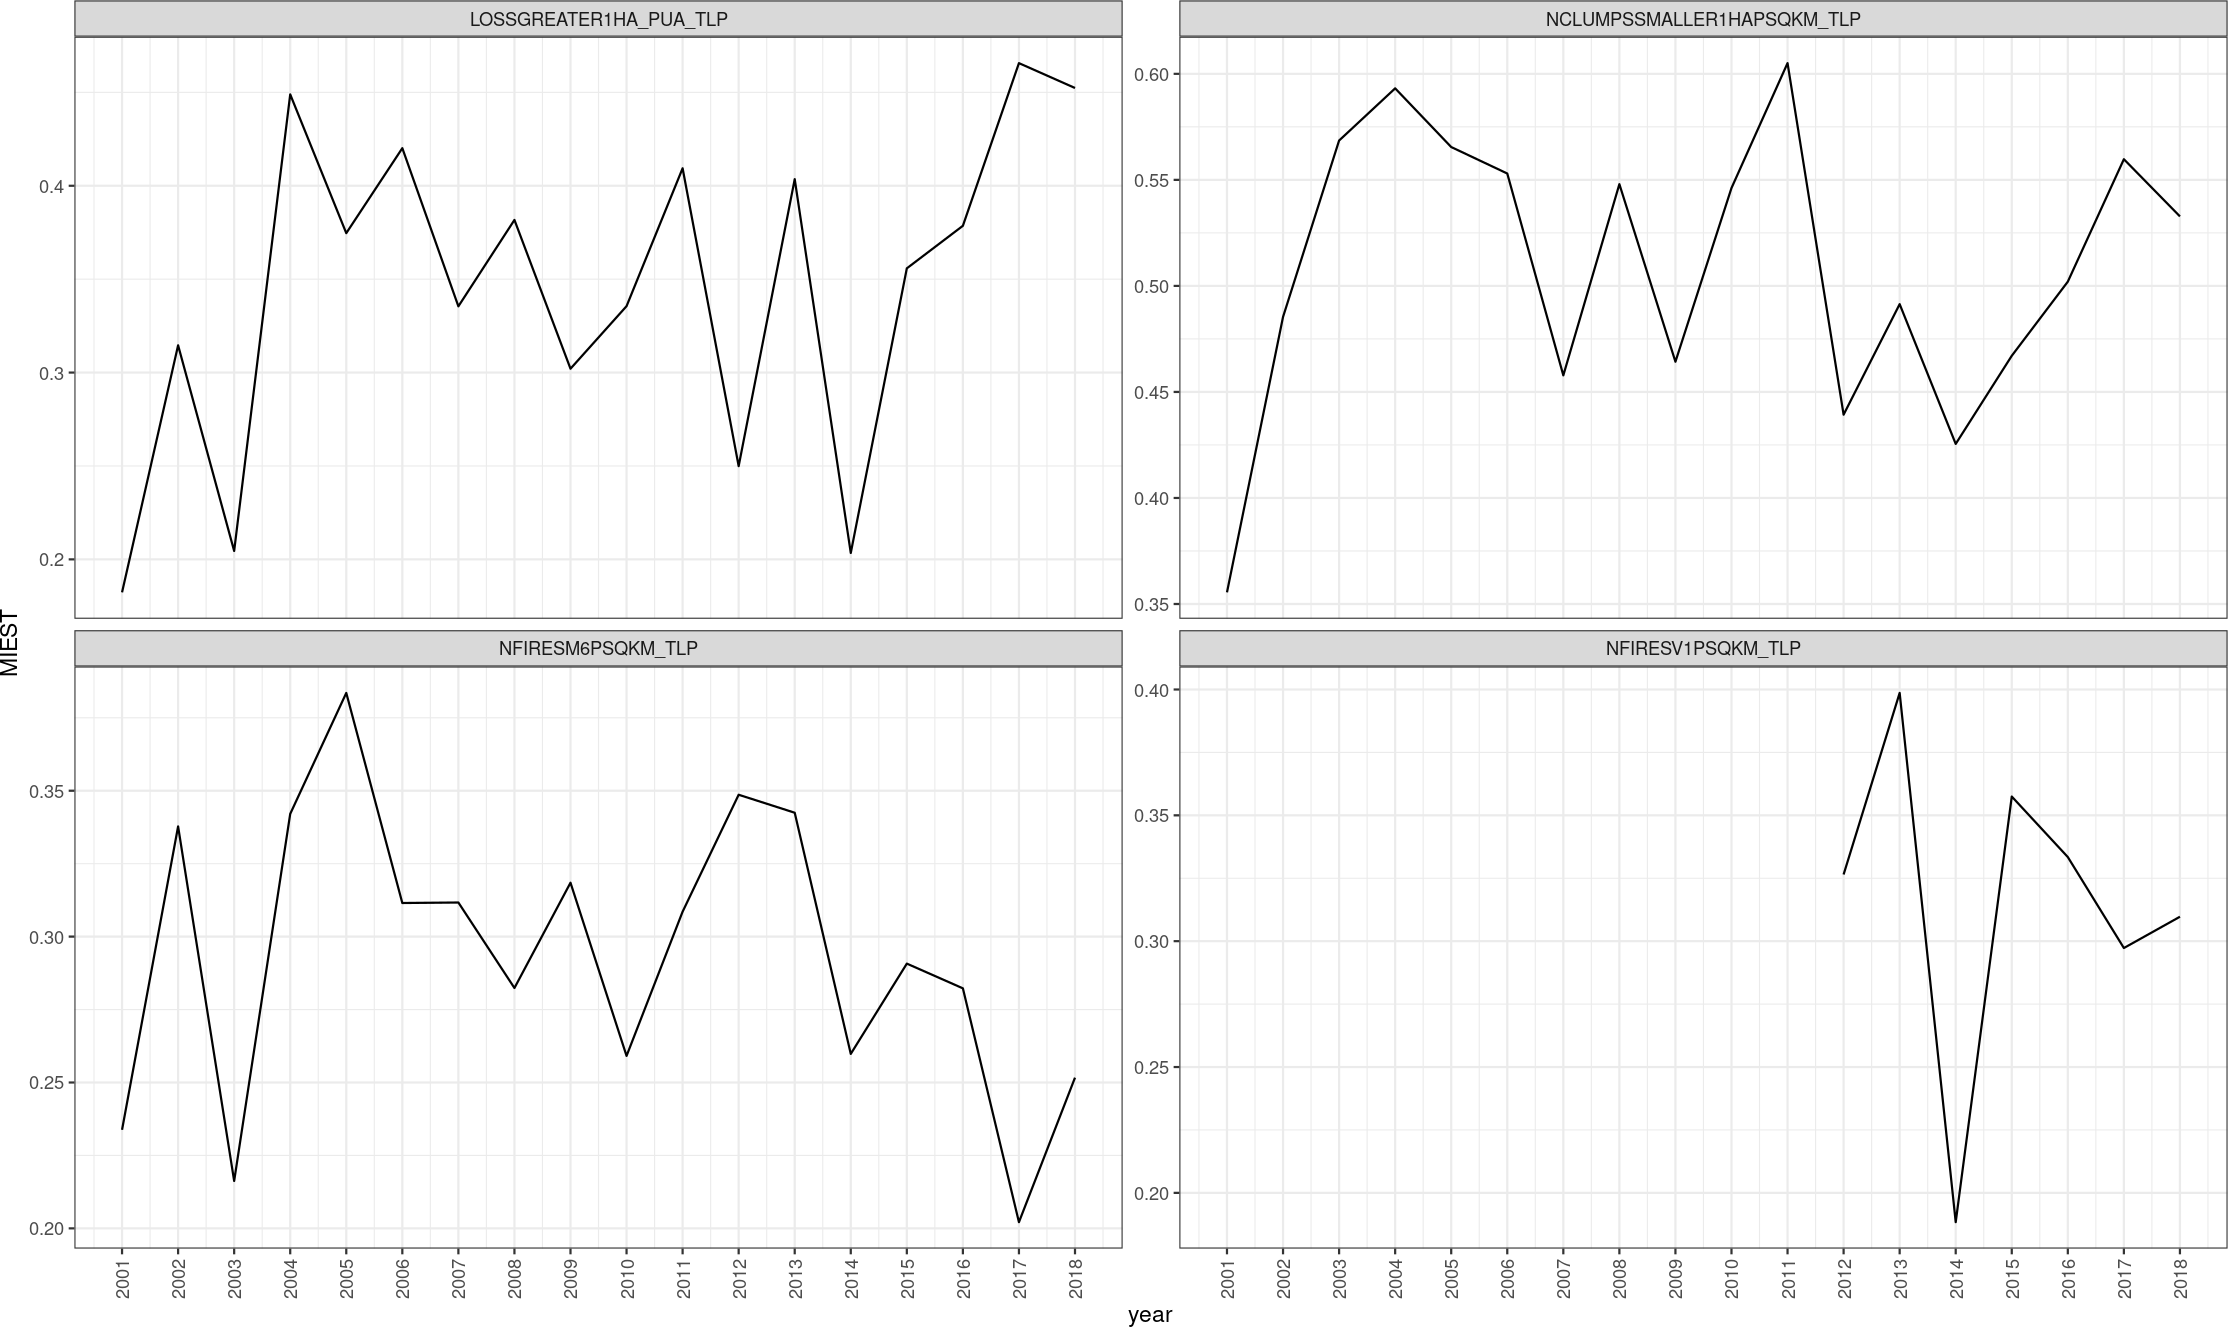
\includegraphics{img/modelling/transformations-1} \end{center}

\begin{Shaded}
\begin{Highlighting}[]
\CommentTok{\# jpeg(\textquotesingle{}out/morans\_i\_time\_series\_four\_variables\_tlp.jpg\textquotesingle{}, width = 3840, height = 1600, res = 350)}
\NormalTok{lambda\_tests }\SpecialCharTok{\%\textgreater{}\%} 
\NormalTok{  dplyr}\SpecialCharTok{::}\FunctionTok{select}\NormalTok{(}\AttributeTok{value =}\NormalTok{ MIEST, MIVAR, LENGTH, variable2, year) }\SpecialCharTok{\%\textgreater{}\%} 
  \FunctionTok{mutate}\NormalTok{(}\AttributeTok{year\_factor =} \FunctionTok{factor}\NormalTok{(year)) }\SpecialCharTok{\%\textgreater{}\%} 
    \FunctionTok{mutate}\NormalTok{(}\AttributeTok{variable =} \FunctionTok{case\_when}\NormalTok{(}
\NormalTok{    variable2 }\SpecialCharTok{==} \StringTok{\textquotesingle{}NFIRESM6PSQKM\_TLP\textquotesingle{}} \SpecialCharTok{\textasciitilde{}} \StringTok{\textquotesingle{}(C)\textquotesingle{}}\NormalTok{,}
\NormalTok{    variable2 }\SpecialCharTok{==} \StringTok{\textquotesingle{}NFIRESV1PSQKM\_TLP\textquotesingle{}} \SpecialCharTok{\textasciitilde{}} \StringTok{\textquotesingle{}(D)\textquotesingle{}}\NormalTok{,}
\NormalTok{    variable2 }\SpecialCharTok{==} \StringTok{\textquotesingle{}NCLUMPSSMALLER1HAPSQKM\_TLP\textquotesingle{}} \SpecialCharTok{\textasciitilde{}} \StringTok{\textquotesingle{}(B)\textquotesingle{}}\NormalTok{,}
\NormalTok{    variable2 }\SpecialCharTok{==} \StringTok{\textquotesingle{}LOSSGREATER1HA\_PUA\_TLP\textquotesingle{}} \SpecialCharTok{\textasciitilde{}} \StringTok{\textquotesingle{}(A)\textquotesingle{}}
\NormalTok{    )) }\SpecialCharTok{\%\textgreater{}\%} 
\NormalTok{  ggplot }\SpecialCharTok{+}
  \FunctionTok{aes}\NormalTok{(}\AttributeTok{x =}\NormalTok{ year\_factor, }\AttributeTok{y =}\NormalTok{ value, }\AttributeTok{group =}\NormalTok{ variable, }\AttributeTok{color =}\NormalTok{ variable) }\SpecialCharTok{+}
  \FunctionTok{theme\_bw}\NormalTok{() }\SpecialCharTok{+}
  \FunctionTok{theme}\NormalTok{(}
    \AttributeTok{axis.text.x =} \FunctionTok{element\_text}\NormalTok{(}\AttributeTok{angle =} \DecValTok{90}\NormalTok{, }\AttributeTok{vjust =} \FloatTok{0.5}\NormalTok{),}
    \AttributeTok{panel.grid.minor =} \FunctionTok{element\_blank}\NormalTok{(),}
    \AttributeTok{text =} \FunctionTok{element\_text}\NormalTok{(}\AttributeTok{size =} \DecValTok{14}\NormalTok{), }\AttributeTok{aspect.ratio =} \DecValTok{1}\SpecialCharTok{/}\DecValTok{3}\NormalTok{) }\SpecialCharTok{+}
  \FunctionTok{geom\_line}\NormalTok{(}\AttributeTok{lwd =} \FloatTok{0.6}\NormalTok{) }\SpecialCharTok{+}
  \FunctionTok{geom\_errorbar}\NormalTok{(}
    \FunctionTok{aes}\NormalTok{(}
      \AttributeTok{ymin =}\NormalTok{ value }\SpecialCharTok{{-}} \FunctionTok{qnorm}\NormalTok{(}\AttributeTok{p=}\NormalTok{(}\FloatTok{0.05}\SpecialCharTok{/}\DecValTok{2}\NormalTok{)}\SpecialCharTok{+}\NormalTok{(}\DecValTok{1}\FloatTok{{-}0.05}\NormalTok{))}\SpecialCharTok{*}\FunctionTok{sqrt}\NormalTok{(MIVAR)}\SpecialCharTok{/}\FunctionTok{sqrt}\NormalTok{(LENGTH),}
      \AttributeTok{ymax =}\NormalTok{ value }\SpecialCharTok{+} \FunctionTok{qnorm}\NormalTok{(}\AttributeTok{p=}\NormalTok{(}\FloatTok{0.05}\SpecialCharTok{/}\DecValTok{2}\NormalTok{)}\SpecialCharTok{+}\NormalTok{(}\DecValTok{1}\FloatTok{{-}0.05}\NormalTok{))}\SpecialCharTok{*}\FunctionTok{sqrt}\NormalTok{(MIVAR)}\SpecialCharTok{/}\FunctionTok{sqrt}\NormalTok{(LENGTH)),}
      \CommentTok{\#color = variable),}
    \AttributeTok{alpha =} \FloatTok{0.75}\NormalTok{,}
    \AttributeTok{colour =} \StringTok{"grey50"}\NormalTok{,}
    \AttributeTok{width =}\NormalTok{ .}\DecValTok{1}\NormalTok{) }\SpecialCharTok{+}
  \FunctionTok{geom\_point}\NormalTok{(}\AttributeTok{size=}\FloatTok{0.5}\NormalTok{, }\AttributeTok{shape=}\DecValTok{21}\NormalTok{) }\SpecialCharTok{+} 
  \FunctionTok{xlab}\NormalTok{(}\StringTok{\textquotesingle{}Year\textquotesingle{}}\NormalTok{) }\SpecialCharTok{+}
  \FunctionTok{ylab}\NormalTok{(}\StringTok{"Moran\textquotesingle{}s I"}\NormalTok{)}
\end{Highlighting}
\end{Shaded}

\begin{center}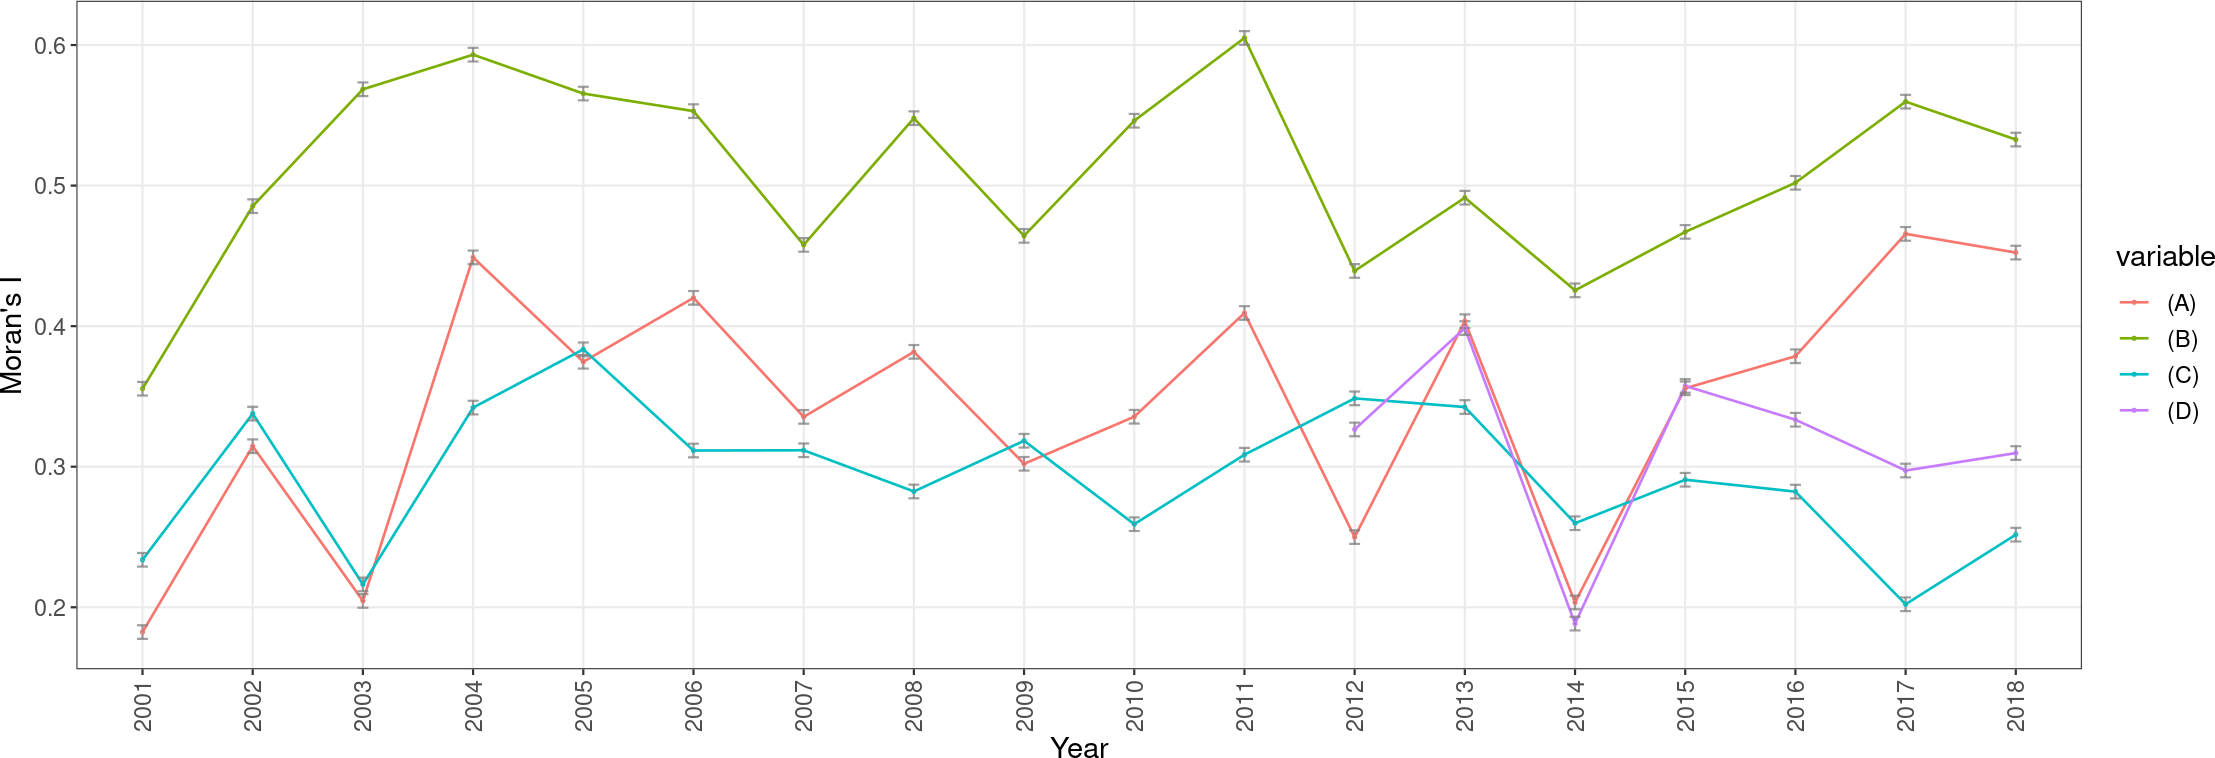
\includegraphics{img/modelling/transformations-2} \end{center}

\begin{Shaded}
\begin{Highlighting}[]
\CommentTok{\# dev.off()}
\end{Highlighting}
\end{Shaded}

\hypertarget{lisa-maps}{%
\subsection{LISA maps}\label{lisa-maps}}

\begin{Shaded}
\begin{Highlighting}[]
\CommentTok{\# Large clearings}
\NormalTok{loss1hagreatercols }\OtherTok{\textless{}{-}} \FunctionTok{grep}\NormalTok{(}\StringTok{"\^{}YEAR[0{-}9]\{,2\}\_LOSS.*\_TLP$"}\NormalTok{, }\FunctionTok{names}\NormalTok{(hexzonalfmt), }\AttributeTok{value =}\NormalTok{ T)}
\NormalTok{hexlisamaps }\OtherTok{\textless{}{-}} \FunctionTok{map}\NormalTok{(loss1hagreatercols, }\ControlFlowTok{function}\NormalTok{(x) \{}
\NormalTok{    lm }\OtherTok{\textless{}{-}} \FunctionTok{lisamap}\NormalTok{(}\AttributeTok{objesp =}\NormalTok{ hexzonalfmt, }\AttributeTok{var =}\NormalTok{ x, }\AttributeTok{pesos =}\NormalTok{ hexww, }\AttributeTok{tituloleyenda =} \StringTok{"Significance}\SpecialCharTok{\textbackslash{}n}\StringTok{(}\SpecialCharTok{\textbackslash{}"}\StringTok{x{-}y}\SpecialCharTok{\textbackslash{}"}\StringTok{, read as}\SpecialCharTok{\textbackslash{}n}\StringTok{ }\SpecialCharTok{\textbackslash{}"}\StringTok{x}\SpecialCharTok{\textbackslash{}"}\StringTok{ surrounded}\SpecialCharTok{\textbackslash{}n}\StringTok{by }\SpecialCharTok{\textbackslash{}"}\StringTok{y}\SpecialCharTok{\textbackslash{}"}\StringTok{"}\NormalTok{,}
        \AttributeTok{leyenda =}\NormalTok{ T, }\AttributeTok{anchuratitulo =} \DecValTok{1000}\NormalTok{, }\AttributeTok{tamanotitulo =} \DecValTok{14}\NormalTok{, }\AttributeTok{fuentedatos =} \StringTok{"Hansen et al., 2013"}\NormalTok{,}
        \AttributeTok{titulomapa =} \FunctionTok{paste0}\NormalTok{(}\DecValTok{2000} \SpecialCharTok{+} \FunctionTok{as.numeric}\NormalTok{(}\FunctionTok{create\_year\_from\_string}\NormalTok{(x))))}
\NormalTok{    lm}\SpecialCharTok{$}\NormalTok{grafico}\SpecialCharTok{$}\NormalTok{layers }\OtherTok{\textless{}{-}} \FunctionTok{c}\NormalTok{(lm}\SpecialCharTok{$}\NormalTok{grafico}\SpecialCharTok{$}\NormalTok{layers, }\FunctionTok{geom\_sf}\NormalTok{(}\AttributeTok{data =}\NormalTok{ seaocean, }\AttributeTok{fill =} \StringTok{"white"}\NormalTok{)[[}\DecValTok{1}\NormalTok{]])}
    \FunctionTok{return}\NormalTok{(lm}\SpecialCharTok{$}\NormalTok{grafico)}
\NormalTok{\})}
\NormalTok{legendhexlisamaps }\OtherTok{\textless{}{-}} \FunctionTok{get\_legend}\NormalTok{(hexlisamaps[[}\DecValTok{1}\NormalTok{]] }\SpecialCharTok{+} \FunctionTok{guides}\NormalTok{(}\AttributeTok{color =} \FunctionTok{guide\_legend}\NormalTok{(}\AttributeTok{nrow =} \DecValTok{1}\NormalTok{)) }\SpecialCharTok{+}
    \FunctionTok{theme}\NormalTok{(}\AttributeTok{legend.position =} \StringTok{"bottom"}\NormalTok{))}
\NormalTok{hexlisamapsnl }\OtherTok{\textless{}{-}} \FunctionTok{map}\NormalTok{(hexlisamaps, }\ControlFlowTok{function}\NormalTok{(x) \{}
\NormalTok{    mapRange }\OtherTok{\textless{}{-}} \FunctionTok{c}\NormalTok{(}\FunctionTok{range}\NormalTok{(}\FunctionTok{st\_coordinates}\NormalTok{(hexzonalfmt)[, }\DecValTok{1}\NormalTok{]), }\FunctionTok{range}\NormalTok{(}\FunctionTok{st\_coordinates}\NormalTok{(hexzonalfmt)[,}
        \DecValTok{2}\NormalTok{]))}
\NormalTok{    x }\SpecialCharTok{+} \FunctionTok{theme}\NormalTok{(}\AttributeTok{legend.position =} \StringTok{"none"}\NormalTok{) }\SpecialCharTok{+} \FunctionTok{labs}\NormalTok{(}\AttributeTok{caption =} \ConstantTok{NULL}\NormalTok{) }\SpecialCharTok{+} \FunctionTok{coord\_sf}\NormalTok{(}\AttributeTok{xlim =}\NormalTok{ mapRange[}\FunctionTok{c}\NormalTok{(}\DecValTok{1}\SpecialCharTok{:}\DecValTok{2}\NormalTok{)],}
        \AttributeTok{ylim =}\NormalTok{ mapRange[}\FunctionTok{c}\NormalTok{(}\DecValTok{3}\SpecialCharTok{:}\DecValTok{4}\NormalTok{)]) }\SpecialCharTok{+} \FunctionTok{theme}\NormalTok{(}\AttributeTok{plot.title =} \FunctionTok{element\_text}\NormalTok{(}\AttributeTok{hjust =} \FloatTok{0.5}\NormalTok{, }\AttributeTok{vjust =} \SpecialCharTok{{-}}\FloatTok{0.5}\NormalTok{,}
        \AttributeTok{size =} \DecValTok{12}\NormalTok{), }\AttributeTok{plot.background =} \FunctionTok{element\_rect}\NormalTok{(}\AttributeTok{fill =} \StringTok{"white"}\NormalTok{, }\AttributeTok{color =} \StringTok{"black"}\NormalTok{,}
        \AttributeTok{size =} \DecValTok{0}\NormalTok{), }\AttributeTok{axis.text =} \FunctionTok{element\_blank}\NormalTok{(), }\AttributeTok{axis.ticks =} \FunctionTok{element\_blank}\NormalTok{(), }\AttributeTok{plot.margin =} \FunctionTok{unit}\NormalTok{(}\FunctionTok{c}\NormalTok{(}\DecValTok{2}\NormalTok{,}
        \DecValTok{2}\NormalTok{, }\DecValTok{2}\NormalTok{, }\DecValTok{2}\NormalTok{), }\StringTok{"mm"}\NormalTok{))}
\NormalTok{\})}
\CommentTok{\# jpeg(\textquotesingle{}out/yearly\_lisamaps\_forestloss1ha\_tlp.jpg\textquotesingle{}, width = 3840, height =}
\CommentTok{\# 1600, res = 350)}
\FunctionTok{plot\_grid}\NormalTok{(}\AttributeTok{plotlist =}\NormalTok{ hexlisamapsnl, }\AttributeTok{nrow =} \DecValTok{3}\NormalTok{)}
\end{Highlighting}
\end{Shaded}

\begin{center}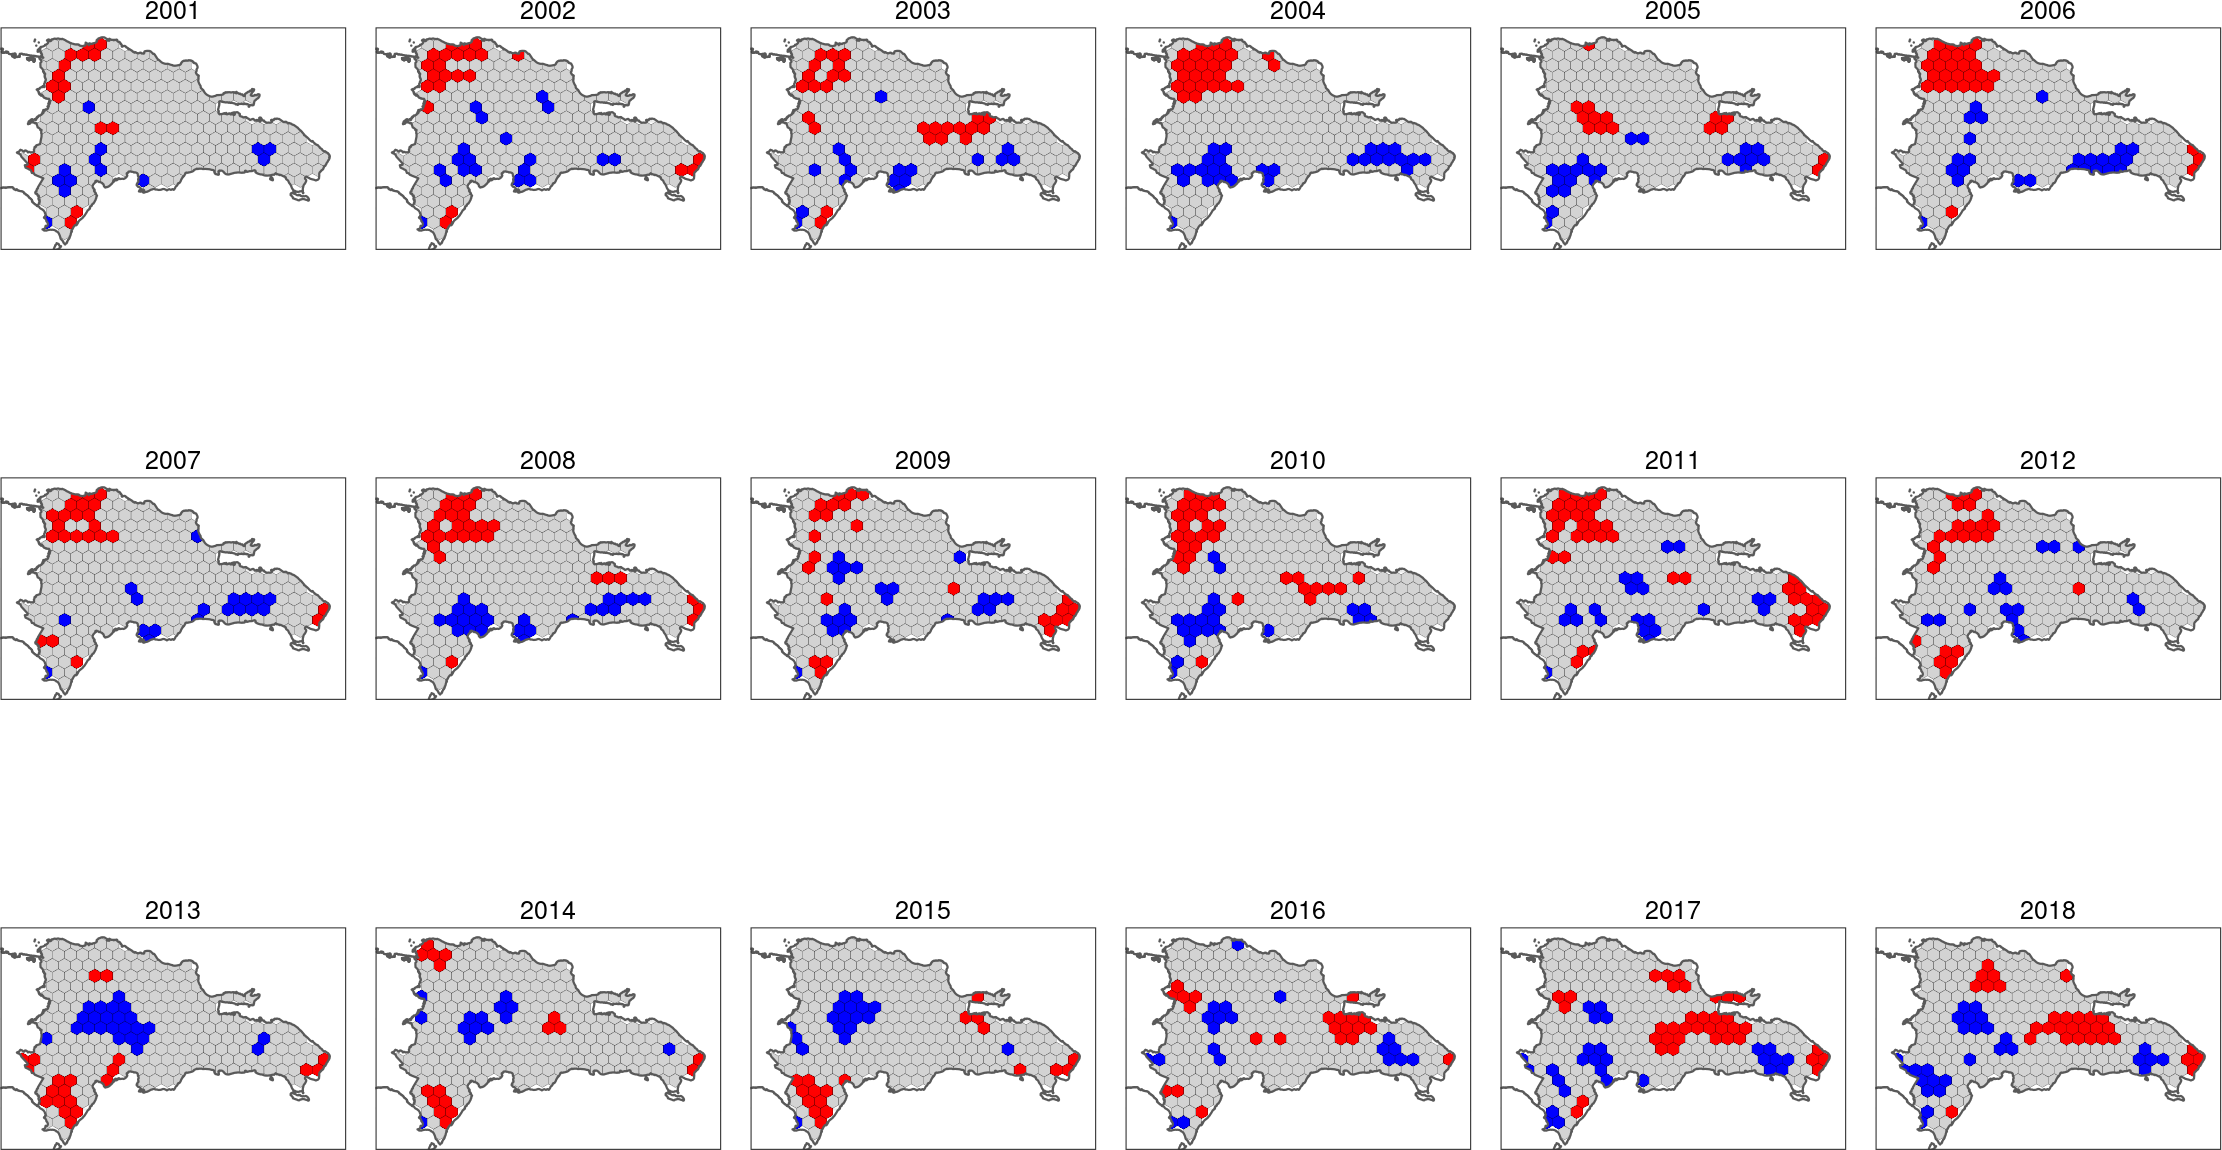
\includegraphics{img/modelling/aa-lisa-maps-1} \end{center}

\begin{Shaded}
\begin{Highlighting}[]
\CommentTok{\# dev.off()}

\CommentTok{\# Small clearings}
\NormalTok{nclumpssmall1hacols }\OtherTok{\textless{}{-}} \FunctionTok{grep}\NormalTok{(}\StringTok{"\^{}NCLUMPSSMALLER1HA\_YEAR[0{-}9]\{,2\}.*\_TLP$"}\NormalTok{, }\FunctionTok{names}\NormalTok{(hexzonalfmt),}
    \AttributeTok{value =}\NormalTok{ T)}
\NormalTok{hexlisamapssmal1ha }\OtherTok{\textless{}{-}} \FunctionTok{map}\NormalTok{(nclumpssmall1hacols, }\ControlFlowTok{function}\NormalTok{(x) \{}
\NormalTok{    lm }\OtherTok{\textless{}{-}} \FunctionTok{lisamap}\NormalTok{(}\AttributeTok{objesp =}\NormalTok{ hexzonalfmt, }\AttributeTok{var =}\NormalTok{ x, }\AttributeTok{pesos =}\NormalTok{ hexww, }\AttributeTok{tituloleyenda =} \StringTok{"Significance}\SpecialCharTok{\textbackslash{}n}\StringTok{(}\SpecialCharTok{\textbackslash{}"}\StringTok{x{-}y}\SpecialCharTok{\textbackslash{}"}\StringTok{, read as}\SpecialCharTok{\textbackslash{}n}\StringTok{ }\SpecialCharTok{\textbackslash{}"}\StringTok{x}\SpecialCharTok{\textbackslash{}"}\StringTok{ surrounded}\SpecialCharTok{\textbackslash{}n}\StringTok{by }\SpecialCharTok{\textbackslash{}"}\StringTok{y}\SpecialCharTok{\textbackslash{}"}\StringTok{"}\NormalTok{,}
        \AttributeTok{leyenda =}\NormalTok{ T, }\AttributeTok{anchuratitulo =} \DecValTok{1000}\NormalTok{, }\AttributeTok{tamanotitulo =} \DecValTok{14}\NormalTok{, }\AttributeTok{fuentedatos =} \StringTok{"Hansen et al., 2013"}\NormalTok{,}
        \AttributeTok{titulomapa =} \FunctionTok{paste0}\NormalTok{(}\DecValTok{2000} \SpecialCharTok{+} \FunctionTok{as.numeric}\NormalTok{(}\FunctionTok{create\_year\_from\_string}\NormalTok{(x))))}
\NormalTok{    lm}\SpecialCharTok{$}\NormalTok{grafico}\SpecialCharTok{$}\NormalTok{layers }\OtherTok{\textless{}{-}} \FunctionTok{c}\NormalTok{(lm}\SpecialCharTok{$}\NormalTok{grafico}\SpecialCharTok{$}\NormalTok{layers, }\FunctionTok{geom\_sf}\NormalTok{(}\AttributeTok{data =}\NormalTok{ seaocean, }\AttributeTok{fill =} \StringTok{"white"}\NormalTok{)[[}\DecValTok{1}\NormalTok{]])}
    \FunctionTok{return}\NormalTok{(lm}\SpecialCharTok{$}\NormalTok{grafico)}
\NormalTok{\})}
\NormalTok{legendhexlisamapssmal1ha }\OtherTok{\textless{}{-}} \FunctionTok{get\_legend}\NormalTok{(hexlisamapssmal1ha[[}\DecValTok{1}\NormalTok{]] }\SpecialCharTok{+} \FunctionTok{guides}\NormalTok{(}\AttributeTok{color =} \FunctionTok{guide\_legend}\NormalTok{(}\AttributeTok{nrow =} \DecValTok{1}\NormalTok{)) }\SpecialCharTok{+}
    \FunctionTok{theme}\NormalTok{(}\AttributeTok{legend.position =} \StringTok{"bottom"}\NormalTok{))}
\NormalTok{hexlisamapsnlsmal1ha }\OtherTok{\textless{}{-}} \FunctionTok{map}\NormalTok{(hexlisamapssmal1ha, }\ControlFlowTok{function}\NormalTok{(x) \{}
\NormalTok{    mapRange }\OtherTok{\textless{}{-}} \FunctionTok{c}\NormalTok{(}\FunctionTok{range}\NormalTok{(}\FunctionTok{st\_coordinates}\NormalTok{(hexzonalfmt)[, }\DecValTok{1}\NormalTok{]), }\FunctionTok{range}\NormalTok{(}\FunctionTok{st\_coordinates}\NormalTok{(hexzonalfmt)[,}
        \DecValTok{2}\NormalTok{]))}
\NormalTok{    x }\SpecialCharTok{+} \FunctionTok{theme}\NormalTok{(}\AttributeTok{legend.position =} \StringTok{"none"}\NormalTok{) }\SpecialCharTok{+} \FunctionTok{labs}\NormalTok{(}\AttributeTok{caption =} \ConstantTok{NULL}\NormalTok{) }\SpecialCharTok{+} \FunctionTok{coord\_sf}\NormalTok{(}\AttributeTok{xlim =}\NormalTok{ mapRange[}\FunctionTok{c}\NormalTok{(}\DecValTok{1}\SpecialCharTok{:}\DecValTok{2}\NormalTok{)],}
        \AttributeTok{ylim =}\NormalTok{ mapRange[}\FunctionTok{c}\NormalTok{(}\DecValTok{3}\SpecialCharTok{:}\DecValTok{4}\NormalTok{)]) }\SpecialCharTok{+} \FunctionTok{theme}\NormalTok{(}\AttributeTok{plot.title =} \FunctionTok{element\_text}\NormalTok{(}\AttributeTok{hjust =} \FloatTok{0.5}\NormalTok{, }\AttributeTok{vjust =} \SpecialCharTok{{-}}\FloatTok{0.5}\NormalTok{,}
        \AttributeTok{size =} \DecValTok{12}\NormalTok{), }\AttributeTok{plot.background =} \FunctionTok{element\_rect}\NormalTok{(}\AttributeTok{fill =} \StringTok{"white"}\NormalTok{, }\AttributeTok{color =} \StringTok{"black"}\NormalTok{,}
        \AttributeTok{size =} \DecValTok{0}\NormalTok{), }\AttributeTok{axis.text =} \FunctionTok{element\_blank}\NormalTok{(), }\AttributeTok{axis.ticks =} \FunctionTok{element\_blank}\NormalTok{(), }\AttributeTok{plot.margin =} \FunctionTok{unit}\NormalTok{(}\FunctionTok{c}\NormalTok{(}\DecValTok{2}\NormalTok{,}
        \DecValTok{2}\NormalTok{, }\DecValTok{2}\NormalTok{, }\DecValTok{2}\NormalTok{), }\StringTok{"mm"}\NormalTok{))}
\NormalTok{\})}
\CommentTok{\# jpeg(\textquotesingle{}out/yearly\_lisamaps\_nclumpssmaller1ha\_tlp.jpg\textquotesingle{}, width = 3840, height =}
\CommentTok{\# 1600, res = 350)}
\FunctionTok{plot\_grid}\NormalTok{(}\AttributeTok{plotlist =}\NormalTok{ hexlisamapsnlsmal1ha, }\AttributeTok{nrow =} \DecValTok{3}\NormalTok{)}
\end{Highlighting}
\end{Shaded}

\begin{center}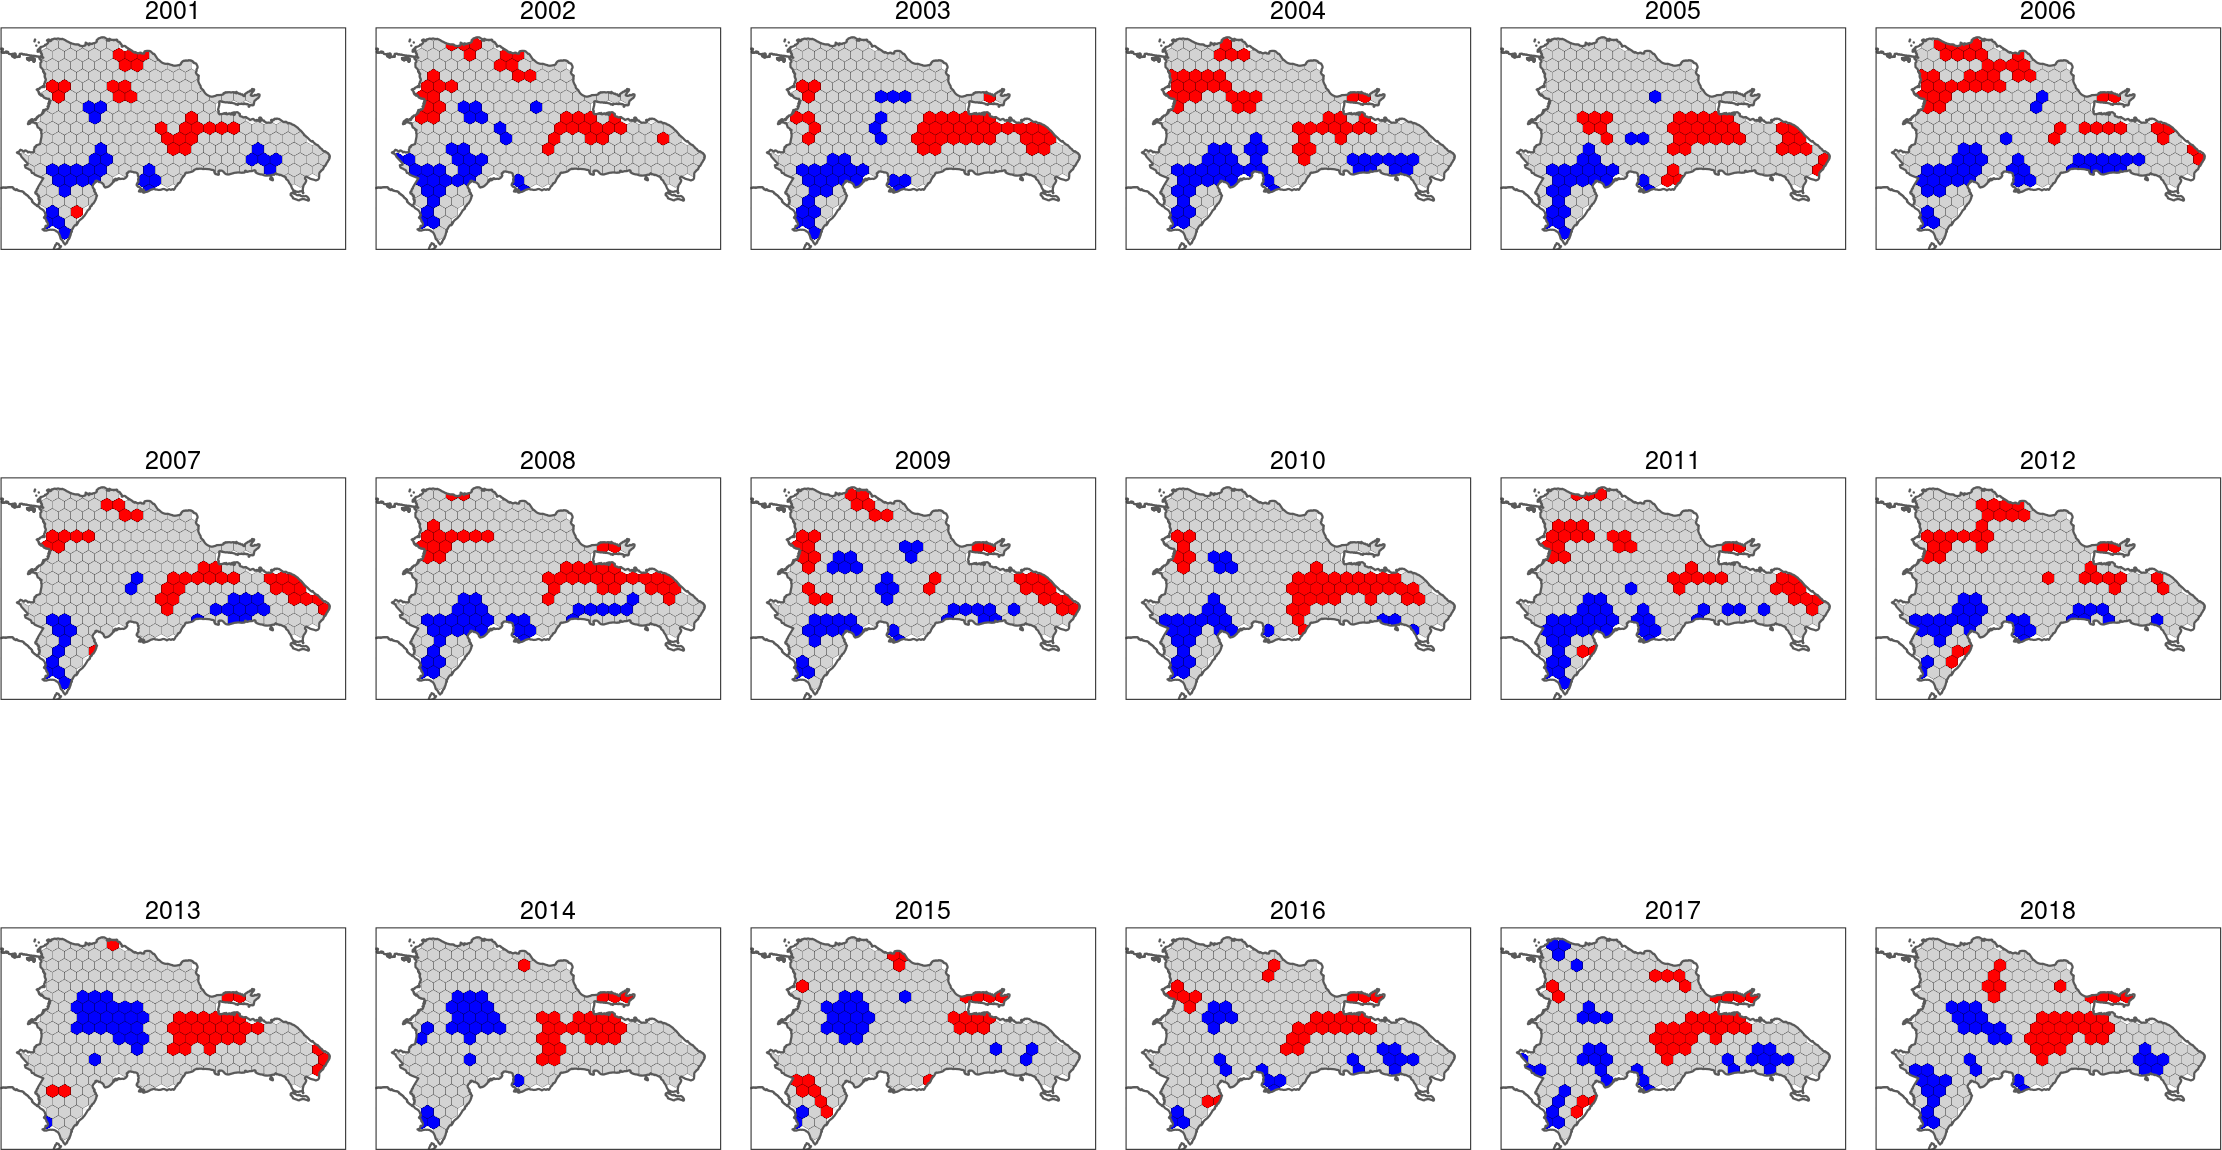
\includegraphics{img/modelling/aa-lisa-maps-2} \end{center}

\begin{Shaded}
\begin{Highlighting}[]
\CommentTok{\# dev.off()}

\CommentTok{\# Fire points MODIS}
\NormalTok{firemodiscols }\OtherTok{\textless{}{-}} \FunctionTok{grep}\NormalTok{(}\StringTok{"\^{}NFIRESM6\_YEAR[0{-}9]\{,2\}.*\_TLP$"}\NormalTok{, }\FunctionTok{names}\NormalTok{(hexzonalfmt), }\AttributeTok{value =}\NormalTok{ T)}
\NormalTok{hexlisamapsfiremodis }\OtherTok{\textless{}{-}} \FunctionTok{map}\NormalTok{(firemodiscols, }\ControlFlowTok{function}\NormalTok{(x) \{}
\NormalTok{    lm }\OtherTok{\textless{}{-}} \FunctionTok{lisamap}\NormalTok{(}\AttributeTok{objesp =}\NormalTok{ hexzonalfmt, }\AttributeTok{var =}\NormalTok{ x, }\AttributeTok{pesos =}\NormalTok{ hexww, }\AttributeTok{tituloleyenda =} \StringTok{"Significance}\SpecialCharTok{\textbackslash{}n}\StringTok{(}\SpecialCharTok{\textbackslash{}"}\StringTok{x{-}y}\SpecialCharTok{\textbackslash{}"}\StringTok{, read as}\SpecialCharTok{\textbackslash{}n}\StringTok{ }\SpecialCharTok{\textbackslash{}"}\StringTok{x}\SpecialCharTok{\textbackslash{}"}\StringTok{ surrounded}\SpecialCharTok{\textbackslash{}n}\StringTok{by }\SpecialCharTok{\textbackslash{}"}\StringTok{y}\SpecialCharTok{\textbackslash{}"}\StringTok{"}\NormalTok{,}
        \AttributeTok{leyenda =}\NormalTok{ T, }\AttributeTok{anchuratitulo =} \DecValTok{1000}\NormalTok{, }\AttributeTok{tamanotitulo =} \DecValTok{14}\NormalTok{, }\AttributeTok{fuentedatos =} \StringTok{"Hansen et al., 2013"}\NormalTok{,}
        \AttributeTok{titulomapa =} \FunctionTok{paste0}\NormalTok{(}\DecValTok{2000} \SpecialCharTok{+} \FunctionTok{as.numeric}\NormalTok{(}\FunctionTok{create\_year\_from\_string}\NormalTok{(x))))}
\NormalTok{    lm}\SpecialCharTok{$}\NormalTok{grafico}\SpecialCharTok{$}\NormalTok{layers }\OtherTok{\textless{}{-}} \FunctionTok{c}\NormalTok{(lm}\SpecialCharTok{$}\NormalTok{grafico}\SpecialCharTok{$}\NormalTok{layers, }\FunctionTok{geom\_sf}\NormalTok{(}\AttributeTok{data =}\NormalTok{ seaocean, }\AttributeTok{fill =} \StringTok{"white"}\NormalTok{)[[}\DecValTok{1}\NormalTok{]])}
    \FunctionTok{return}\NormalTok{(lm}\SpecialCharTok{$}\NormalTok{grafico)}
\NormalTok{\})}
\NormalTok{legendhexlisamapsfiremodis }\OtherTok{\textless{}{-}} \FunctionTok{get\_legend}\NormalTok{(hexlisamapsfiremodis[[}\DecValTok{1}\NormalTok{]] }\SpecialCharTok{+} \FunctionTok{guides}\NormalTok{(}\AttributeTok{color =} \FunctionTok{guide\_legend}\NormalTok{(}\AttributeTok{nrow =} \DecValTok{1}\NormalTok{)) }\SpecialCharTok{+}
    \FunctionTok{theme}\NormalTok{(}\AttributeTok{legend.position =} \StringTok{"bottom"}\NormalTok{))}
\NormalTok{hexlisamapsnlfiremodis }\OtherTok{\textless{}{-}} \FunctionTok{map}\NormalTok{(hexlisamapsfiremodis, }\ControlFlowTok{function}\NormalTok{(x) \{}
\NormalTok{    mapRange }\OtherTok{\textless{}{-}} \FunctionTok{c}\NormalTok{(}\FunctionTok{range}\NormalTok{(}\FunctionTok{st\_coordinates}\NormalTok{(hexzonalfmt)[, }\DecValTok{1}\NormalTok{]), }\FunctionTok{range}\NormalTok{(}\FunctionTok{st\_coordinates}\NormalTok{(hexzonalfmt)[,}
        \DecValTok{2}\NormalTok{]))}
\NormalTok{    x }\SpecialCharTok{+} \FunctionTok{theme}\NormalTok{(}\AttributeTok{legend.position =} \StringTok{"none"}\NormalTok{) }\SpecialCharTok{+} \FunctionTok{labs}\NormalTok{(}\AttributeTok{caption =} \ConstantTok{NULL}\NormalTok{) }\SpecialCharTok{+} \FunctionTok{coord\_sf}\NormalTok{(}\AttributeTok{xlim =}\NormalTok{ mapRange[}\FunctionTok{c}\NormalTok{(}\DecValTok{1}\SpecialCharTok{:}\DecValTok{2}\NormalTok{)],}
        \AttributeTok{ylim =}\NormalTok{ mapRange[}\FunctionTok{c}\NormalTok{(}\DecValTok{3}\SpecialCharTok{:}\DecValTok{4}\NormalTok{)]) }\SpecialCharTok{+} \FunctionTok{theme}\NormalTok{(}\AttributeTok{plot.title =} \FunctionTok{element\_text}\NormalTok{(}\AttributeTok{hjust =} \FloatTok{0.5}\NormalTok{, }\AttributeTok{vjust =} \SpecialCharTok{{-}}\FloatTok{0.5}\NormalTok{,}
        \AttributeTok{size =} \DecValTok{12}\NormalTok{), }\AttributeTok{plot.background =} \FunctionTok{element\_rect}\NormalTok{(}\AttributeTok{fill =} \StringTok{"white"}\NormalTok{, }\AttributeTok{color =} \StringTok{"black"}\NormalTok{,}
        \AttributeTok{size =} \DecValTok{0}\NormalTok{), }\AttributeTok{axis.text =} \FunctionTok{element\_blank}\NormalTok{(), }\AttributeTok{axis.ticks =} \FunctionTok{element\_blank}\NormalTok{(), }\AttributeTok{plot.margin =} \FunctionTok{unit}\NormalTok{(}\FunctionTok{c}\NormalTok{(}\DecValTok{2}\NormalTok{,}
        \DecValTok{2}\NormalTok{, }\DecValTok{2}\NormalTok{, }\DecValTok{2}\NormalTok{), }\StringTok{"mm"}\NormalTok{))}
\NormalTok{\})}
\CommentTok{\# jpeg(\textquotesingle{}out/yearly\_lisamaps\_firemodis\_tlp.jpg\textquotesingle{}, width = 3840, height = 1600,}
\CommentTok{\# res = 350)}
\FunctionTok{plot\_grid}\NormalTok{(}\AttributeTok{plotlist =}\NormalTok{ hexlisamapsnlfiremodis, }\AttributeTok{nrow =} \DecValTok{3}\NormalTok{)}
\end{Highlighting}
\end{Shaded}

\begin{center}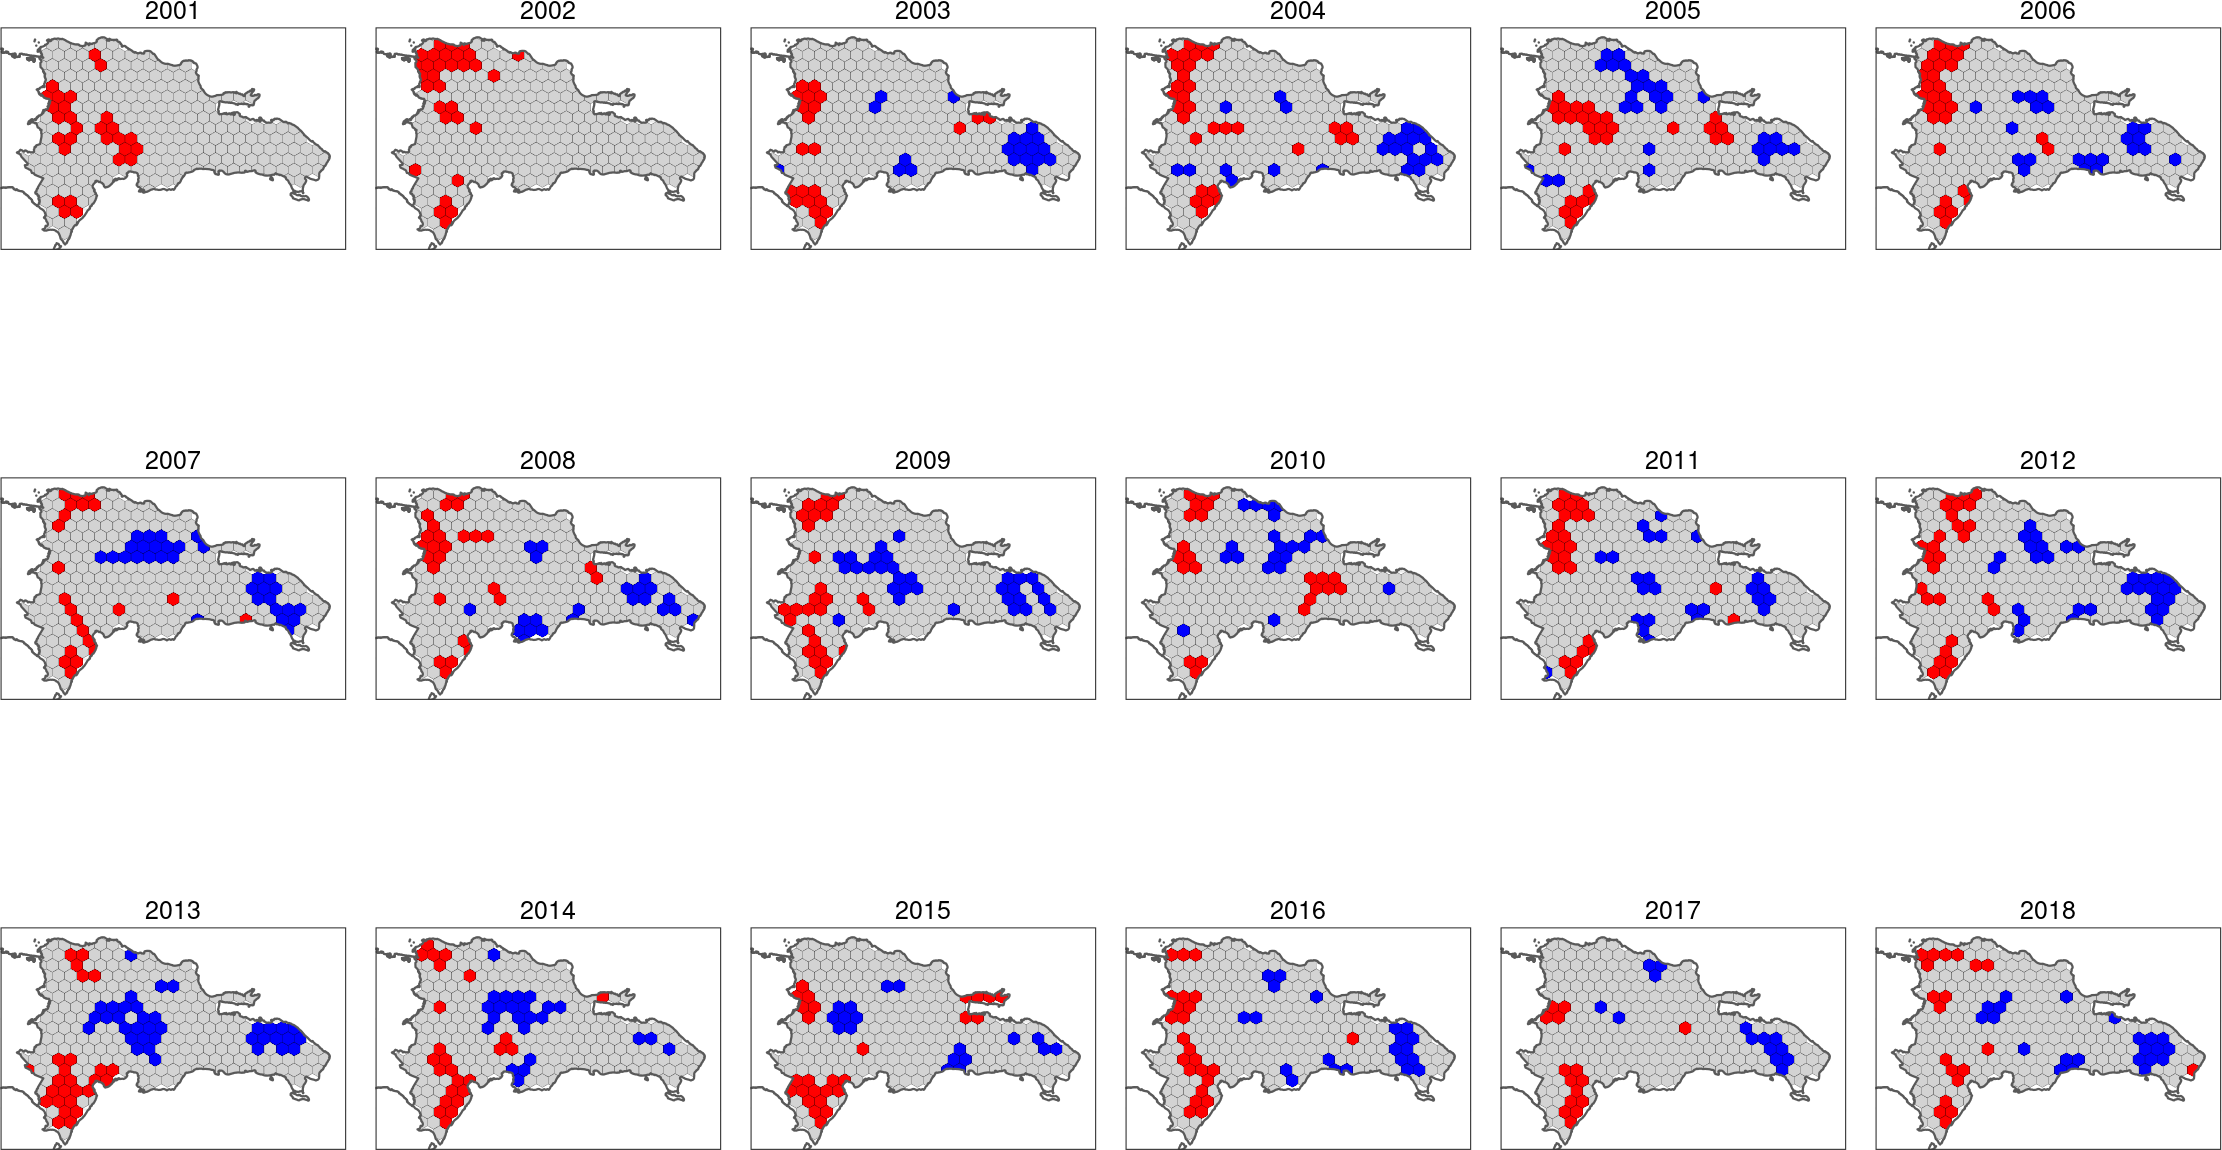
\includegraphics{img/modelling/aa-lisa-maps-3} \end{center}

\begin{Shaded}
\begin{Highlighting}[]
\CommentTok{\# dev.off()}

\CommentTok{\# Fire points VIIRS}
\NormalTok{fireviirscols }\OtherTok{\textless{}{-}} \FunctionTok{grep}\NormalTok{(}\StringTok{"\^{}NFIRESV1\_YEAR[0{-}9]\{,2\}.*\_TLP$"}\NormalTok{, }\FunctionTok{names}\NormalTok{(hexzonalfmt), }\AttributeTok{value =}\NormalTok{ T)}
\NormalTok{hexlisamapsfireviirs }\OtherTok{\textless{}{-}} \FunctionTok{map}\NormalTok{(fireviirscols, }\ControlFlowTok{function}\NormalTok{(x) \{}
\NormalTok{    lm }\OtherTok{\textless{}{-}} \FunctionTok{lisamap}\NormalTok{(}\AttributeTok{objesp =}\NormalTok{ hexzonalfmt, }\AttributeTok{var =}\NormalTok{ x, }\AttributeTok{pesos =}\NormalTok{ hexww, }\AttributeTok{tituloleyenda =} \StringTok{"Significance}\SpecialCharTok{\textbackslash{}n}\StringTok{(}\SpecialCharTok{\textbackslash{}"}\StringTok{x{-}y}\SpecialCharTok{\textbackslash{}"}\StringTok{, read as}\SpecialCharTok{\textbackslash{}n}\StringTok{ }\SpecialCharTok{\textbackslash{}"}\StringTok{x}\SpecialCharTok{\textbackslash{}"}\StringTok{ surrounded}\SpecialCharTok{\textbackslash{}n}\StringTok{by }\SpecialCharTok{\textbackslash{}"}\StringTok{y}\SpecialCharTok{\textbackslash{}"}\StringTok{"}\NormalTok{,}
        \AttributeTok{leyenda =}\NormalTok{ T, }\AttributeTok{anchuratitulo =} \DecValTok{1000}\NormalTok{, }\AttributeTok{tamanotitulo =} \DecValTok{14}\NormalTok{, }\AttributeTok{fuentedatos =} \StringTok{"Hansen et al., 2013"}\NormalTok{,}
        \AttributeTok{titulomapa =} \FunctionTok{paste0}\NormalTok{(}\DecValTok{2000} \SpecialCharTok{+} \FunctionTok{as.numeric}\NormalTok{(}\FunctionTok{create\_year\_from\_string}\NormalTok{(x))))}
\NormalTok{    lm}\SpecialCharTok{$}\NormalTok{grafico}\SpecialCharTok{$}\NormalTok{layers }\OtherTok{\textless{}{-}} \FunctionTok{c}\NormalTok{(lm}\SpecialCharTok{$}\NormalTok{grafico}\SpecialCharTok{$}\NormalTok{layers, }\FunctionTok{geom\_sf}\NormalTok{(}\AttributeTok{data =}\NormalTok{ seaocean, }\AttributeTok{fill =} \StringTok{"white"}\NormalTok{)[[}\DecValTok{1}\NormalTok{]])}
    \FunctionTok{return}\NormalTok{(lm}\SpecialCharTok{$}\NormalTok{grafico)}
\NormalTok{\})}
\NormalTok{legendhexlisamapsfireviirs }\OtherTok{\textless{}{-}} \FunctionTok{get\_legend}\NormalTok{(hexlisamapsfireviirs[[}\DecValTok{1}\NormalTok{]] }\SpecialCharTok{+} \FunctionTok{guides}\NormalTok{(}\AttributeTok{color =} \FunctionTok{guide\_legend}\NormalTok{(}\AttributeTok{nrow =} \DecValTok{1}\NormalTok{)) }\SpecialCharTok{+}
    \FunctionTok{theme}\NormalTok{(}\AttributeTok{legend.position =} \StringTok{"bottom"}\NormalTok{))}
\NormalTok{hexlisamapsnlfireviirs }\OtherTok{\textless{}{-}} \FunctionTok{map}\NormalTok{(hexlisamapsfireviirs, }\ControlFlowTok{function}\NormalTok{(x) \{}
\NormalTok{    mapRange }\OtherTok{\textless{}{-}} \FunctionTok{c}\NormalTok{(}\FunctionTok{range}\NormalTok{(}\FunctionTok{st\_coordinates}\NormalTok{(hexzonalfmt)[, }\DecValTok{1}\NormalTok{]), }\FunctionTok{range}\NormalTok{(}\FunctionTok{st\_coordinates}\NormalTok{(hexzonalfmt)[,}
        \DecValTok{2}\NormalTok{]))}
\NormalTok{    x }\SpecialCharTok{+} \FunctionTok{theme}\NormalTok{(}\AttributeTok{legend.position =} \StringTok{"none"}\NormalTok{) }\SpecialCharTok{+} \FunctionTok{labs}\NormalTok{(}\AttributeTok{caption =} \ConstantTok{NULL}\NormalTok{) }\SpecialCharTok{+} \FunctionTok{coord\_sf}\NormalTok{(}\AttributeTok{xlim =}\NormalTok{ mapRange[}\FunctionTok{c}\NormalTok{(}\DecValTok{1}\SpecialCharTok{:}\DecValTok{2}\NormalTok{)],}
        \AttributeTok{ylim =}\NormalTok{ mapRange[}\FunctionTok{c}\NormalTok{(}\DecValTok{3}\SpecialCharTok{:}\DecValTok{4}\NormalTok{)]) }\SpecialCharTok{+} \FunctionTok{theme}\NormalTok{(}\AttributeTok{plot.title =} \FunctionTok{element\_text}\NormalTok{(}\AttributeTok{hjust =} \FloatTok{0.5}\NormalTok{, }\AttributeTok{vjust =} \SpecialCharTok{{-}}\FloatTok{0.5}\NormalTok{,}
        \AttributeTok{size =} \DecValTok{12}\NormalTok{), }\AttributeTok{plot.background =} \FunctionTok{element\_rect}\NormalTok{(}\AttributeTok{fill =} \StringTok{"white"}\NormalTok{, }\AttributeTok{color =} \StringTok{"black"}\NormalTok{,}
        \AttributeTok{size =} \DecValTok{0}\NormalTok{), }\AttributeTok{axis.text =} \FunctionTok{element\_blank}\NormalTok{(), }\AttributeTok{axis.ticks =} \FunctionTok{element\_blank}\NormalTok{(), }\AttributeTok{plot.margin =} \FunctionTok{unit}\NormalTok{(}\FunctionTok{c}\NormalTok{(}\DecValTok{2}\NormalTok{,}
        \DecValTok{2}\NormalTok{, }\DecValTok{2}\NormalTok{, }\DecValTok{2}\NormalTok{), }\StringTok{"mm"}\NormalTok{))}
\NormalTok{\})}
\CommentTok{\# jpeg(\textquotesingle{}out/yearly\_lisamaps\_fireviirs\_tlp.jpg\textquotesingle{}, width = 3840, height = 1600,}
\CommentTok{\# res = 350)}
\FunctionTok{plot\_grid}\NormalTok{(}\AttributeTok{plotlist =}\NormalTok{ hexlisamapsnlfireviirs, }\AttributeTok{nrow =} \DecValTok{2}\NormalTok{, }\AttributeTok{ncol =} \DecValTok{4}\NormalTok{)}
\end{Highlighting}
\end{Shaded}

\begin{center}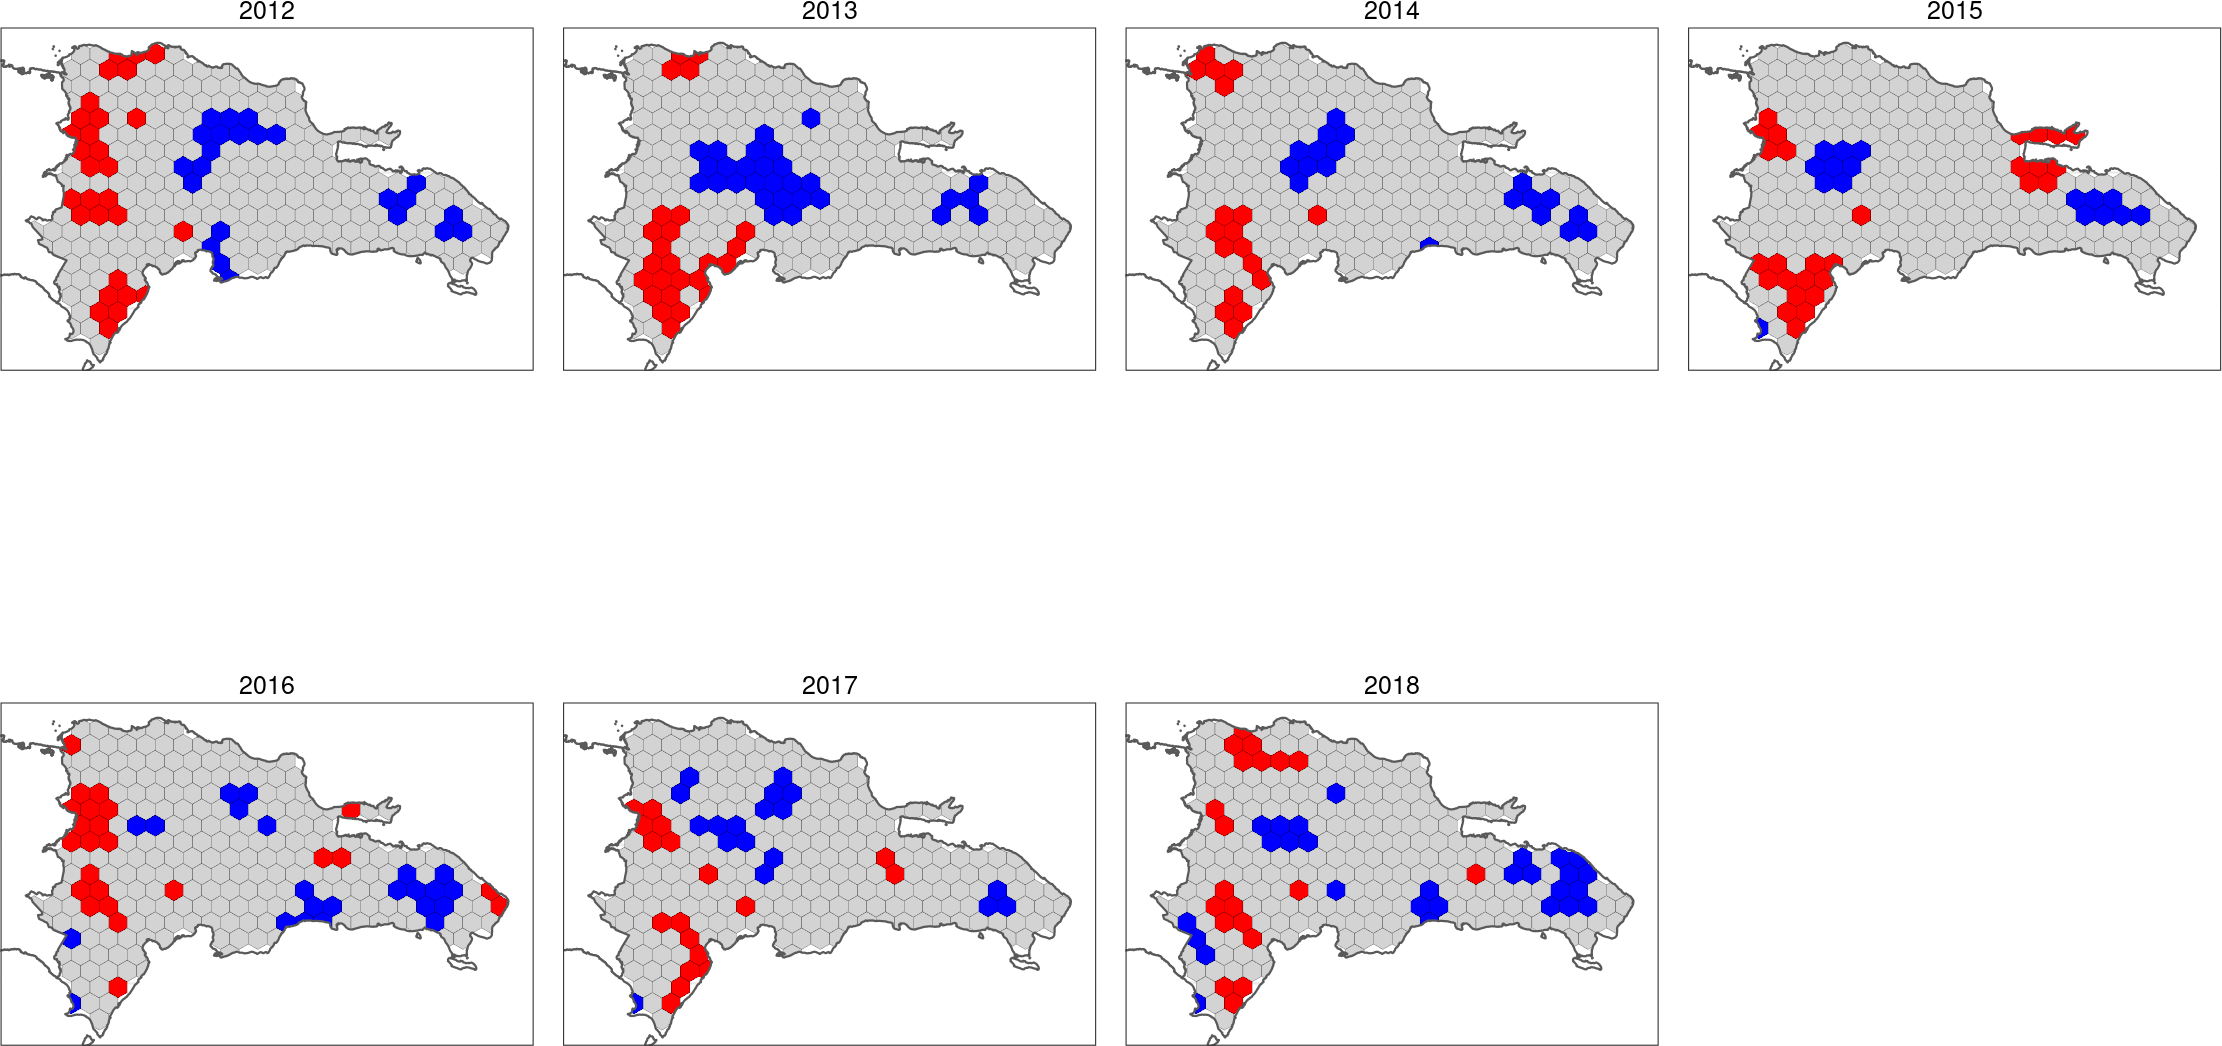
\includegraphics{img/modelling/aa-lisa-maps-4} \end{center}

\begin{Shaded}
\begin{Highlighting}[]
\CommentTok{\# dev.off()}
\end{Highlighting}
\end{Shaded}

\hypertarget{models}{%
\subsection{Models}\label{models}}

\begin{Shaded}
\begin{Highlighting}[]
\CommentTok{\# LARGE CLEARINGS TRANS}
\NormalTok{annual\_models\_folossg1ha\_trans\_formulas }\OtherTok{\textless{}{-}} \FunctionTok{data.frame}\NormalTok{(}\AttributeTok{y =} \FunctionTok{grep}\NormalTok{(}\StringTok{"\^{}YEAR[0{-}9]\{,2\}\_LOSS.*\_TLP$"}\NormalTok{,}
    \FunctionTok{names}\NormalTok{(hexzonalfmt), }\AttributeTok{value =}\NormalTok{ T), }\AttributeTok{x =} \FunctionTok{grep}\NormalTok{(}\StringTok{"\^{}NFIRESM6\_YEAR[0{-}9]\{,2\}.*\_TLP$"}\NormalTok{, }\FunctionTok{names}\NormalTok{(hexzonalfmt),}
    \AttributeTok{value =}\NormalTok{ T)) }\SpecialCharTok{\%\textgreater{}\%}
    \FunctionTok{mutate}\NormalTok{(}\AttributeTok{formula =} \FunctionTok{paste}\NormalTok{(y, x, }\AttributeTok{sep =} \StringTok{" \textasciitilde{} "}\NormalTok{)) }\SpecialCharTok{\%\textgreater{}\%}
    \FunctionTok{pull}\NormalTok{(formula)}
\NormalTok{annual\_models\_folossg1ha\_trans }\OtherTok{\textless{}{-}} \FunctionTok{sapply}\NormalTok{(annual\_models\_folossg1ha\_trans\_formulas,}
    \ControlFlowTok{function}\NormalTok{(x) hexzonalfmt }\SpecialCharTok{\%\textgreater{}\%}
        \FunctionTok{st\_drop\_geometry}\NormalTok{() }\SpecialCharTok{\%\textgreater{}\%}
        \FunctionTok{replace}\NormalTok{(}\FunctionTok{is.na}\NormalTok{(.), }\DecValTok{0}\NormalTok{) }\SpecialCharTok{\%\textgreater{}\%}
\NormalTok{        spatialreg}\SpecialCharTok{::}\FunctionTok{errorsarlm}\NormalTok{(}\AttributeTok{formula =}\NormalTok{ x, }\AttributeTok{data =}\NormalTok{ ., }\AttributeTok{listw =}\NormalTok{ hexww), }\AttributeTok{simplify =}\NormalTok{ F)}
\FunctionTok{lapply}\NormalTok{(annual\_models\_folossg1ha\_trans, }\ControlFlowTok{function}\NormalTok{(x) }\FunctionTok{summary}\NormalTok{(x, }\AttributeTok{Nagelkerke =}\NormalTok{ T))}
\DocumentationTok{\#\# $\textasciigrave{}YEAR1\_LOSSGREATER1HA\_PUA\_TLP \textasciitilde{} NFIRESM6\_YEAR1\_PSQKM\_TLP\textasciigrave{}}
\DocumentationTok{\#\# }
\DocumentationTok{\#\# Call:spatialreg::errorsarlm(formula = x, data = ., listw = hexww)}
\DocumentationTok{\#\# }
\DocumentationTok{\#\# Residuals:}
\DocumentationTok{\#\#        Min         1Q     Median         3Q        Max }
\DocumentationTok{\#\# {-}0.0851811 {-}0.0228101  0.0003949  0.0240279  0.1214120 }
\DocumentationTok{\#\# }
\DocumentationTok{\#\# Type: error }
\DocumentationTok{\#\# Coefficients: (asymptotic standard errors) }
\DocumentationTok{\#\#                           Estimate Std. Error z value  Pr(\textgreater{}|z|)}
\DocumentationTok{\#\# (Intercept)              0.0711969  0.0036501 19.5056 \textless{} 2.2e{-}16}
\DocumentationTok{\#\# NFIRESM6\_YEAR1\_PSQKM\_TLP 0.1530253  0.0169809  9.0116 \textless{} 2.2e{-}16}
\DocumentationTok{\#\# }
\DocumentationTok{\#\# Lambda: 0.30186, LR test value: 12.096, p{-}value: 0.00050525}
\DocumentationTok{\#\# Asymptotic standard error: 0.085745}
\DocumentationTok{\#\#     z{-}value: 3.5204, p{-}value: 0.00043088}
\DocumentationTok{\#\# Wald statistic: 12.393, p{-}value: 0.00043088}
\DocumentationTok{\#\# }
\DocumentationTok{\#\# Log likelihood: 478.7628 for error model}
\DocumentationTok{\#\# ML residual variance (sigma squared): 0.0013045, (sigma: 0.036118)}
\DocumentationTok{\#\# Nagelkerke pseudo{-}R{-}squared: 0.29212 }
\DocumentationTok{\#\# Number of observations: 253 }
\DocumentationTok{\#\# Number of parameters estimated: 4 }
\DocumentationTok{\#\# AIC: {-}949.53, (AIC for lm: {-}939.43)}
\DocumentationTok{\#\# }
\DocumentationTok{\#\# }
\DocumentationTok{\#\# $\textasciigrave{}YEAR2\_LOSSGREATER1HA\_PUA\_TLP \textasciitilde{} NFIRESM6\_YEAR2\_PSQKM\_TLP\textasciigrave{}}
\DocumentationTok{\#\# }
\DocumentationTok{\#\# Call:spatialreg::errorsarlm(formula = x, data = ., listw = hexww)}
\DocumentationTok{\#\# }
\DocumentationTok{\#\# Residuals:}
\DocumentationTok{\#\#         Min          1Q      Median          3Q         Max }
\DocumentationTok{\#\# {-}0.08064020 {-}0.01935483 {-}0.00014982  0.02103636  0.12272537 }
\DocumentationTok{\#\# }
\DocumentationTok{\#\# Type: error }
\DocumentationTok{\#\# Coefficients: (asymptotic standard errors) }
\DocumentationTok{\#\#                           Estimate Std. Error z value  Pr(\textgreater{}|z|)}
\DocumentationTok{\#\# (Intercept)              0.0714086  0.0043518 16.4089 \textless{} 2.2e{-}16}
\DocumentationTok{\#\# NFIRESM6\_YEAR2\_PSQKM\_TLP 0.1706985  0.0206797  8.2544  2.22e{-}16}
\DocumentationTok{\#\# }
\DocumentationTok{\#\# Lambda: 0.44757, LR test value: 30.037, p{-}value: 4.2382e{-}08}
\DocumentationTok{\#\# Asymptotic standard error: 0.07595}
\DocumentationTok{\#\#     z{-}value: 5.8929, p{-}value: 3.7956e{-}09}
\DocumentationTok{\#\# Wald statistic: 34.726, p{-}value: 3.7956e{-}09}
\DocumentationTok{\#\# }
\DocumentationTok{\#\# Log likelihood: 488.6127 for error model}
\DocumentationTok{\#\# ML residual variance (sigma squared): 0.001176, (sigma: 0.034292)}
\DocumentationTok{\#\# Nagelkerke pseudo{-}R{-}squared: 0.34462 }
\DocumentationTok{\#\# Number of observations: 253 }
\DocumentationTok{\#\# Number of parameters estimated: 4 }
\DocumentationTok{\#\# AIC: {-}969.23, (AIC for lm: {-}941.19)}
\DocumentationTok{\#\# }
\DocumentationTok{\#\# }
\DocumentationTok{\#\# $\textasciigrave{}YEAR3\_LOSSGREATER1HA\_PUA\_TLP \textasciitilde{} NFIRESM6\_YEAR3\_PSQKM\_TLP\textasciigrave{}}
\DocumentationTok{\#\# }
\DocumentationTok{\#\# Call:spatialreg::errorsarlm(formula = x, data = ., listw = hexww)}
\DocumentationTok{\#\# }
\DocumentationTok{\#\# Residuals:}
\DocumentationTok{\#\#        Min         1Q     Median         3Q        Max }
\DocumentationTok{\#\# {-}0.0720108 {-}0.0178344  0.0015545  0.0161489  0.1136078 }
\DocumentationTok{\#\# }
\DocumentationTok{\#\# Type: error }
\DocumentationTok{\#\# Coefficients: (asymptotic standard errors) }
\DocumentationTok{\#\#                           Estimate Std. Error z value  Pr(\textgreater{}|z|)}
\DocumentationTok{\#\# (Intercept)              0.0484404  0.0031861  15.204 \textless{} 2.2e{-}16}
\DocumentationTok{\#\# NFIRESM6\_YEAR3\_PSQKM\_TLP 0.1315503  0.0176625   7.448 9.481e{-}14}
\DocumentationTok{\#\# }
\DocumentationTok{\#\# Lambda: 0.33806, LR test value: 16.565, p{-}value: 4.7001e{-}05}
\DocumentationTok{\#\# Asymptotic standard error: 0.083521}
\DocumentationTok{\#\#     z{-}value: 4.0476, p{-}value: 5.1742e{-}05}
\DocumentationTok{\#\# Wald statistic: 16.383, p{-}value: 5.1742e{-}05}
\DocumentationTok{\#\# }
\DocumentationTok{\#\# Log likelihood: 546.945 for error model}
\DocumentationTok{\#\# ML residual variance (sigma squared): 0.00075698, (sigma: 0.027513)}
\DocumentationTok{\#\# Nagelkerke pseudo{-}R{-}squared: 0.24375 }
\DocumentationTok{\#\# Number of observations: 253 }
\DocumentationTok{\#\# Number of parameters estimated: 4 }
\DocumentationTok{\#\# AIC: {-}1085.9, (AIC for lm: {-}1071.3)}
\DocumentationTok{\#\# }
\DocumentationTok{\#\# }
\DocumentationTok{\#\# $\textasciigrave{}YEAR4\_LOSSGREATER1HA\_PUA\_TLP \textasciitilde{} NFIRESM6\_YEAR4\_PSQKM\_TLP\textasciigrave{}}
\DocumentationTok{\#\# }
\DocumentationTok{\#\# Call:spatialreg::errorsarlm(formula = x, data = ., listw = hexww)}
\DocumentationTok{\#\# }
\DocumentationTok{\#\# Residuals:}
\DocumentationTok{\#\#         Min          1Q      Median          3Q         Max }
\DocumentationTok{\#\# {-}0.10427095 {-}0.02325342 {-}0.00078712  0.02274215  0.12010283 }
\DocumentationTok{\#\# }
\DocumentationTok{\#\# Type: error }
\DocumentationTok{\#\# Coefficients: (asymptotic standard errors) }
\DocumentationTok{\#\#                           Estimate Std. Error z value  Pr(\textgreater{}|z|)}
\DocumentationTok{\#\# (Intercept)              0.0786062  0.0054434 14.4407 \textless{} 2.2e{-}16}
\DocumentationTok{\#\# NFIRESM6\_YEAR4\_PSQKM\_TLP 0.1966704  0.0249289  7.8893 3.109e{-}15}
\DocumentationTok{\#\# }
\DocumentationTok{\#\# Lambda: 0.54909, LR test value: 53.724, p{-}value: 2.307e{-}13}
\DocumentationTok{\#\# Asymptotic standard error: 0.067707}
\DocumentationTok{\#\#     z{-}value: 8.1098, p{-}value: 4.4409e{-}16}
\DocumentationTok{\#\# Wald statistic: 65.77, p{-}value: 5.5511e{-}16}
\DocumentationTok{\#\# }
\DocumentationTok{\#\# Log likelihood: 488.5654 for error model}
\DocumentationTok{\#\# ML residual variance (sigma squared): 0.0011456, (sigma: 0.033846)}
\DocumentationTok{\#\# Nagelkerke pseudo{-}R{-}squared: 0.4292 }
\DocumentationTok{\#\# Number of observations: 253 }
\DocumentationTok{\#\# Number of parameters estimated: 4 }
\DocumentationTok{\#\# AIC: {-}969.13, (AIC for lm: {-}917.41)}
\DocumentationTok{\#\# }
\DocumentationTok{\#\# }
\DocumentationTok{\#\# $\textasciigrave{}YEAR5\_LOSSGREATER1HA\_PUA\_TLP \textasciitilde{} NFIRESM6\_YEAR5\_PSQKM\_TLP\textasciigrave{}}
\DocumentationTok{\#\# }
\DocumentationTok{\#\# Call:spatialreg::errorsarlm(formula = x, data = ., listw = hexww)}
\DocumentationTok{\#\# }
\DocumentationTok{\#\# Residuals:}
\DocumentationTok{\#\#        Min         1Q     Median         3Q        Max }
\DocumentationTok{\#\# {-}0.2200420 {-}0.0264287  0.0024409  0.0349295  0.1950472 }
\DocumentationTok{\#\# }
\DocumentationTok{\#\# Type: error }
\DocumentationTok{\#\# Coefficients: (asymptotic standard errors) }
\DocumentationTok{\#\#                           Estimate Std. Error z value  Pr(\textgreater{}|z|)}
\DocumentationTok{\#\# (Intercept)              0.1536683  0.0091067  16.874 \textless{} 2.2e{-}16}
\DocumentationTok{\#\# NFIRESM6\_YEAR5\_PSQKM\_TLP 0.2705047  0.0204866  13.204 \textless{} 2.2e{-}16}
\DocumentationTok{\#\# }
\DocumentationTok{\#\# Lambda: 0.53713, LR test value: 55.514, p{-}value: 9.2815e{-}14}
\DocumentationTok{\#\# Asymptotic standard error: 0.068744}
\DocumentationTok{\#\#     z{-}value: 7.8135, p{-}value: 5.5511e{-}15}
\DocumentationTok{\#\# Wald statistic: 61.05, p{-}value: 5.5511e{-}15}
\DocumentationTok{\#\# }
\DocumentationTok{\#\# Log likelihood: 362.4219 for error model}
\DocumentationTok{\#\# ML residual variance (sigma squared): 0.0031163, (sigma: 0.055823)}
\DocumentationTok{\#\# Nagelkerke pseudo{-}R{-}squared: 0.54553 }
\DocumentationTok{\#\# Number of observations: 253 }
\DocumentationTok{\#\# Number of parameters estimated: 4 }
\DocumentationTok{\#\# AIC: {-}716.84, (AIC for lm: {-}663.33)}
\DocumentationTok{\#\# }
\DocumentationTok{\#\# }
\DocumentationTok{\#\# $\textasciigrave{}YEAR6\_LOSSGREATER1HA\_PUA\_TLP \textasciitilde{} NFIRESM6\_YEAR6\_PSQKM\_TLP\textasciigrave{}}
\DocumentationTok{\#\# }
\DocumentationTok{\#\# Call:spatialreg::errorsarlm(formula = x, data = ., listw = hexww)}
\DocumentationTok{\#\# }
\DocumentationTok{\#\# Residuals:}
\DocumentationTok{\#\#        Min         1Q     Median         3Q        Max }
\DocumentationTok{\#\# {-}0.0963326 {-}0.0191255 {-}0.0012519  0.0227601  0.1121572 }
\DocumentationTok{\#\# }
\DocumentationTok{\#\# Type: error }
\DocumentationTok{\#\# Coefficients: (asymptotic standard errors) }
\DocumentationTok{\#\#                           Estimate Std. Error z value  Pr(\textgreater{}|z|)}
\DocumentationTok{\#\# (Intercept)              0.0716269  0.0058626  12.218 \textless{} 2.2e{-}16}
\DocumentationTok{\#\# NFIRESM6\_YEAR6\_PSQKM\_TLP 0.2531370  0.0234226  10.807 \textless{} 2.2e{-}16}
\DocumentationTok{\#\# }
\DocumentationTok{\#\# Lambda: 0.57909, LR test value: 65.174, p{-}value: 6.6613e{-}16}
\DocumentationTok{\#\# Asymptotic standard error: 0.065024}
\DocumentationTok{\#\#     z{-}value: 8.9058, p{-}value: \textless{} 2.22e{-}16}
\DocumentationTok{\#\# Wald statistic: 79.313, p{-}value: \textless{} 2.22e{-}16}
\DocumentationTok{\#\# }
\DocumentationTok{\#\# Log likelihood: 481.968 for error model}
\DocumentationTok{\#\# ML residual variance (sigma squared): 0.0011955, (sigma: 0.034576)}
\DocumentationTok{\#\# Nagelkerke pseudo{-}R{-}squared: 0.50288 }
\DocumentationTok{\#\# Number of observations: 253 }
\DocumentationTok{\#\# Number of parameters estimated: 4 }
\DocumentationTok{\#\# AIC: {-}955.94, (AIC for lm: {-}892.76)}
\DocumentationTok{\#\# }
\DocumentationTok{\#\# }
\DocumentationTok{\#\# $\textasciigrave{}YEAR7\_LOSSGREATER1HA\_PUA\_TLP \textasciitilde{} NFIRESM6\_YEAR7\_PSQKM\_TLP\textasciigrave{}}
\DocumentationTok{\#\# }
\DocumentationTok{\#\# Call:spatialreg::errorsarlm(formula = x, data = ., listw = hexww)}
\DocumentationTok{\#\# }
\DocumentationTok{\#\# Residuals:}
\DocumentationTok{\#\#         Min          1Q      Median          3Q         Max }
\DocumentationTok{\#\# {-}0.09177658 {-}0.01870762  0.00035196  0.01959753  0.10222434 }
\DocumentationTok{\#\# }
\DocumentationTok{\#\# Type: error }
\DocumentationTok{\#\# Coefficients: (asymptotic standard errors) }
\DocumentationTok{\#\#                           Estimate Std. Error z value  Pr(\textgreater{}|z|)}
\DocumentationTok{\#\# (Intercept)              0.0694956  0.0049756  13.967 \textless{} 2.2e{-}16}
\DocumentationTok{\#\# NFIRESM6\_YEAR7\_PSQKM\_TLP 0.1936719  0.0188588  10.270 \textless{} 2.2e{-}16}
\DocumentationTok{\#\# }
\DocumentationTok{\#\# Lambda: 0.54926, LR test value: 53.226, p{-}value: 2.9721e{-}13}
\DocumentationTok{\#\# Asymptotic standard error: 0.067692}
\DocumentationTok{\#\#     z{-}value: 8.1141, p{-}value: 4.4409e{-}16}
\DocumentationTok{\#\# Wald statistic: 65.839, p{-}value: 4.4409e{-}16}
\DocumentationTok{\#\# }
\DocumentationTok{\#\# Log likelihood: 508.9855 for error model}
\DocumentationTok{\#\# ML residual variance (sigma squared): 0.00097474, (sigma: 0.031221)}
\DocumentationTok{\#\# Nagelkerke pseudo{-}R{-}squared: 0.43736 }
\DocumentationTok{\#\# Number of observations: 253 }
\DocumentationTok{\#\# Number of parameters estimated: 4 }
\DocumentationTok{\#\# AIC: {-}1010, (AIC for lm: {-}958.74)}
\DocumentationTok{\#\# }
\DocumentationTok{\#\# }
\DocumentationTok{\#\# $\textasciigrave{}YEAR8\_LOSSGREATER1HA\_PUA\_TLP \textasciitilde{} NFIRESM6\_YEAR8\_PSQKM\_TLP\textasciigrave{}}
\DocumentationTok{\#\# }
\DocumentationTok{\#\# Call:spatialreg::errorsarlm(formula = x, data = ., listw = hexww)}
\DocumentationTok{\#\# }
\DocumentationTok{\#\# Residuals:}
\DocumentationTok{\#\#         Min          1Q      Median          3Q         Max }
\DocumentationTok{\#\# {-}0.10941036 {-}0.02081554 {-}0.00082134  0.02227856  0.16290963 }
\DocumentationTok{\#\# }
\DocumentationTok{\#\# Type: error }
\DocumentationTok{\#\# Coefficients: (asymptotic standard errors) }
\DocumentationTok{\#\#                           Estimate Std. Error z value  Pr(\textgreater{}|z|)}
\DocumentationTok{\#\# (Intercept)              0.0854037  0.0070089  12.185 \textless{} 2.2e{-}16}
\DocumentationTok{\#\# NFIRESM6\_YEAR8\_PSQKM\_TLP 0.2304396  0.0206495  11.160 \textless{} 2.2e{-}16}
\DocumentationTok{\#\# }
\DocumentationTok{\#\# Lambda: 0.63283, LR test value: 77.519, p{-}value: \textless{} 2.22e{-}16}
\DocumentationTok{\#\# Asymptotic standard error: 0.059902}
\DocumentationTok{\#\#     z{-}value: 10.565, p{-}value: \textless{} 2.22e{-}16}
\DocumentationTok{\#\# Wald statistic: 111.61, p{-}value: \textless{} 2.22e{-}16}
\DocumentationTok{\#\# }
\DocumentationTok{\#\# Log likelihood: 466.958 for error model}
\DocumentationTok{\#\# ML residual variance (sigma squared): 0.0013204, (sigma: 0.036338)}
\DocumentationTok{\#\# Nagelkerke pseudo{-}R{-}squared: 0.49882 }
\DocumentationTok{\#\# Number of observations: 253 }
\DocumentationTok{\#\# Number of parameters estimated: 4 }
\DocumentationTok{\#\# AIC: {-}925.92, (AIC for lm: {-}850.4)}
\DocumentationTok{\#\# }
\DocumentationTok{\#\# }
\DocumentationTok{\#\# $\textasciigrave{}YEAR9\_LOSSGREATER1HA\_PUA\_TLP \textasciitilde{} NFIRESM6\_YEAR9\_PSQKM\_TLP\textasciigrave{}}
\DocumentationTok{\#\# }
\DocumentationTok{\#\# Call:spatialreg::errorsarlm(formula = x, data = ., listw = hexww)}
\DocumentationTok{\#\# }
\DocumentationTok{\#\# Residuals:}
\DocumentationTok{\#\#       Min        1Q    Median        3Q       Max }
\DocumentationTok{\#\# {-}0.075650 {-}0.022245  0.000197  0.019406  0.195104 }
\DocumentationTok{\#\# }
\DocumentationTok{\#\# Type: error }
\DocumentationTok{\#\# Coefficients: (asymptotic standard errors) }
\DocumentationTok{\#\#                           Estimate Std. Error z value  Pr(\textgreater{}|z|)}
\DocumentationTok{\#\# (Intercept)              0.0678383  0.0052201  12.995 \textless{} 2.2e{-}16}
\DocumentationTok{\#\# NFIRESM6\_YEAR9\_PSQKM\_TLP 0.2156717  0.0187560  11.499 \textless{} 2.2e{-}16}
\DocumentationTok{\#\# }
\DocumentationTok{\#\# Lambda: 0.4962, LR test value: 39.317, p{-}value: 3.602e{-}10}
\DocumentationTok{\#\# Asymptotic standard error: 0.072157}
\DocumentationTok{\#\#     z{-}value: 6.8767, p{-}value: 6.1255e{-}12}
\DocumentationTok{\#\# Wald statistic: 47.289, p{-}value: 6.1257e{-}12}
\DocumentationTok{\#\# }
\DocumentationTok{\#\# Log likelihood: 484.2628 for error model}
\DocumentationTok{\#\# ML residual variance (sigma squared): 0.0012029, (sigma: 0.034683)}
\DocumentationTok{\#\# Nagelkerke pseudo{-}R{-}squared: 0.45071 }
\DocumentationTok{\#\# Number of observations: 253 }
\DocumentationTok{\#\# Number of parameters estimated: 4 }
\DocumentationTok{\#\# AIC: {-}960.53, (AIC for lm: {-}923.21)}
\DocumentationTok{\#\# }
\DocumentationTok{\#\# }
\DocumentationTok{\#\# $\textasciigrave{}YEAR10\_LOSSGREATER1HA\_PUA\_TLP \textasciitilde{} NFIRESM6\_YEAR10\_PSQKM\_TLP\textasciigrave{}}
\DocumentationTok{\#\# }
\DocumentationTok{\#\# Call:spatialreg::errorsarlm(formula = x, data = ., listw = hexww)}
\DocumentationTok{\#\# }
\DocumentationTok{\#\# Residuals:}
\DocumentationTok{\#\#        Min         1Q     Median         3Q        Max }
\DocumentationTok{\#\# {-}0.1162605 {-}0.0212727  0.0018095  0.0232974  0.1840114 }
\DocumentationTok{\#\# }
\DocumentationTok{\#\# Type: error }
\DocumentationTok{\#\# Coefficients: (asymptotic standard errors) }
\DocumentationTok{\#\#                            Estimate Std. Error z value  Pr(\textgreater{}|z|)}
\DocumentationTok{\#\# (Intercept)               0.0848911  0.0053327  15.919 \textless{} 2.2e{-}16}
\DocumentationTok{\#\# NFIRESM6\_YEAR10\_PSQKM\_TLP 0.2317180  0.0219842  10.540 \textless{} 2.2e{-}16}
\DocumentationTok{\#\# }
\DocumentationTok{\#\# Lambda: 0.477, LR test value: 35.899, p{-}value: 2.0786e{-}09}
\DocumentationTok{\#\# Asymptotic standard error: 0.073688}
\DocumentationTok{\#\#     z{-}value: 6.4733, p{-}value: 9.5902e{-}11}
\DocumentationTok{\#\# Wald statistic: 41.903, p{-}value: 9.5902e{-}11}
\DocumentationTok{\#\# }
\DocumentationTok{\#\# Log likelihood: 462.414 for error model}
\DocumentationTok{\#\# ML residual variance (sigma squared): 0.0014366, (sigma: 0.037903)}
\DocumentationTok{\#\# Nagelkerke pseudo{-}R{-}squared: 0.43623 }
\DocumentationTok{\#\# Number of observations: 253 }
\DocumentationTok{\#\# Number of parameters estimated: 4 }
\DocumentationTok{\#\# AIC: {-}916.83, (AIC for lm: {-}882.93)}
\DocumentationTok{\#\# }
\DocumentationTok{\#\# }
\DocumentationTok{\#\# $\textasciigrave{}YEAR11\_LOSSGREATER1HA\_PUA\_TLP \textasciitilde{} NFIRESM6\_YEAR11\_PSQKM\_TLP\textasciigrave{}}
\DocumentationTok{\#\# }
\DocumentationTok{\#\# Call:spatialreg::errorsarlm(formula = x, data = ., listw = hexww)}
\DocumentationTok{\#\# }
\DocumentationTok{\#\# Residuals:}
\DocumentationTok{\#\#        Min         1Q     Median         3Q        Max }
\DocumentationTok{\#\# {-}0.0840600 {-}0.0162287 {-}0.0022334  0.0181762  0.0876676 }
\DocumentationTok{\#\# }
\DocumentationTok{\#\# Type: error }
\DocumentationTok{\#\# Coefficients: (asymptotic standard errors) }
\DocumentationTok{\#\#                            Estimate Std. Error z value  Pr(\textgreater{}|z|)}
\DocumentationTok{\#\# (Intercept)               0.0512135  0.0049629  10.319 \textless{} 2.2e{-}16}
\DocumentationTok{\#\# NFIRESM6\_YEAR11\_PSQKM\_TLP 0.1796224  0.0157287  11.420 \textless{} 2.2e{-}16}
\DocumentationTok{\#\# }
\DocumentationTok{\#\# Lambda: 0.58239, LR test value: 70.556, p{-}value: \textless{} 2.22e{-}16}
\DocumentationTok{\#\# Asymptotic standard error: 0.06472}
\DocumentationTok{\#\#     z{-}value: 8.9986, p{-}value: \textless{} 2.22e{-}16}
\DocumentationTok{\#\# Wald statistic: 80.975, p{-}value: \textless{} 2.22e{-}16}
\DocumentationTok{\#\# }
\DocumentationTok{\#\# Log likelihood: 524.1914 for error model}
\DocumentationTok{\#\# ML residual variance (sigma squared): 0.00085527, (sigma: 0.029245)}
\DocumentationTok{\#\# Nagelkerke pseudo{-}R{-}squared: 0.5089 }
\DocumentationTok{\#\# Number of observations: 253 }
\DocumentationTok{\#\# Number of parameters estimated: 4 }
\DocumentationTok{\#\# AIC: {-}1040.4, (AIC for lm: {-}971.83)}
\DocumentationTok{\#\# }
\DocumentationTok{\#\# }
\DocumentationTok{\#\# $\textasciigrave{}YEAR12\_LOSSGREATER1HA\_PUA\_TLP \textasciitilde{} NFIRESM6\_YEAR12\_PSQKM\_TLP\textasciigrave{}}
\DocumentationTok{\#\# }
\DocumentationTok{\#\# Call:spatialreg::errorsarlm(formula = x, data = ., listw = hexww)}
\DocumentationTok{\#\# }
\DocumentationTok{\#\# Residuals:}
\DocumentationTok{\#\#        Min         1Q     Median         3Q        Max }
\DocumentationTok{\#\# {-}0.1180095 {-}0.0283501  0.0035631  0.0272531  0.1747989 }
\DocumentationTok{\#\# }
\DocumentationTok{\#\# Type: error }
\DocumentationTok{\#\# Coefficients: (asymptotic standard errors) }
\DocumentationTok{\#\#                            Estimate Std. Error z value  Pr(\textgreater{}|z|)}
\DocumentationTok{\#\# (Intercept)               0.0872654  0.0054686  15.957 \textless{} 2.2e{-}16}
\DocumentationTok{\#\# NFIRESM6\_YEAR12\_PSQKM\_TLP 0.2394062  0.0210512  11.373 \textless{} 2.2e{-}16}
\DocumentationTok{\#\# }
\DocumentationTok{\#\# Lambda: 0.39258, LR test value: 22.567, p{-}value: 2.0298e{-}06}
\DocumentationTok{\#\# Asymptotic standard error: 0.079914}
\DocumentationTok{\#\#     z{-}value: 4.9126, p{-}value: 8.9888e{-}07}
\DocumentationTok{\#\# Wald statistic: 24.133, p{-}value: 8.9888e{-}07}
\DocumentationTok{\#\# }
\DocumentationTok{\#\# Log likelihood: 432.7725 for error model}
\DocumentationTok{\#\# ML residual variance (sigma squared): 0.0018493, (sigma: 0.043003)}
\DocumentationTok{\#\# Nagelkerke pseudo{-}R{-}squared: 0.41369 }
\DocumentationTok{\#\# Number of observations: 253 }
\DocumentationTok{\#\# Number of parameters estimated: 4 }
\DocumentationTok{\#\# AIC: {-}857.54, (AIC for lm: {-}836.98)}
\DocumentationTok{\#\# }
\DocumentationTok{\#\# }
\DocumentationTok{\#\# $\textasciigrave{}YEAR13\_LOSSGREATER1HA\_PUA\_TLP \textasciitilde{} NFIRESM6\_YEAR13\_PSQKM\_TLP\textasciigrave{}}
\DocumentationTok{\#\# }
\DocumentationTok{\#\# Call:spatialreg::errorsarlm(formula = x, data = ., listw = hexww)}
\DocumentationTok{\#\# }
\DocumentationTok{\#\# Residuals:}
\DocumentationTok{\#\#        Min         1Q     Median         3Q        Max }
\DocumentationTok{\#\# {-}0.1864478 {-}0.0386916  0.0020771  0.0378961  0.2186490 }
\DocumentationTok{\#\# }
\DocumentationTok{\#\# Type: error }
\DocumentationTok{\#\# Coefficients: (asymptotic standard errors) }
\DocumentationTok{\#\#                            Estimate Std. Error z value  Pr(\textgreater{}|z|)}
\DocumentationTok{\#\# (Intercept)               0.1261562  0.0086123  14.648 \textless{} 2.2e{-}16}
\DocumentationTok{\#\# NFIRESM6\_YEAR13\_PSQKM\_TLP 0.3579929  0.0286252  12.506 \textless{} 2.2e{-}16}
\DocumentationTok{\#\# }
\DocumentationTok{\#\# Lambda: 0.42547, LR test value: 24.296, p{-}value: 8.2629e{-}07}
\DocumentationTok{\#\# Asymptotic standard error: 0.077583}
\DocumentationTok{\#\#     z{-}value: 5.4841, p{-}value: 4.1566e{-}08}
\DocumentationTok{\#\# Wald statistic: 30.075, p{-}value: 4.1566e{-}08}
\DocumentationTok{\#\# }
\DocumentationTok{\#\# Log likelihood: 329.6468 for error model}
\DocumentationTok{\#\# ML residual variance (sigma squared): 0.0041516, (sigma: 0.064433)}
\DocumentationTok{\#\# Nagelkerke pseudo{-}R{-}squared: 0.52467 }
\DocumentationTok{\#\# Number of observations: 253 }
\DocumentationTok{\#\# Number of parameters estimated: 4 }
\DocumentationTok{\#\# AIC: {-}651.29, (AIC for lm: {-}629)}
\DocumentationTok{\#\# }
\DocumentationTok{\#\# }
\DocumentationTok{\#\# $\textasciigrave{}YEAR14\_LOSSGREATER1HA\_PUA\_TLP \textasciitilde{} NFIRESM6\_YEAR14\_PSQKM\_TLP\textasciigrave{}}
\DocumentationTok{\#\# }
\DocumentationTok{\#\# Call:spatialreg::errorsarlm(formula = x, data = ., listw = hexww)}
\DocumentationTok{\#\# }
\DocumentationTok{\#\# Residuals:}
\DocumentationTok{\#\#       Min        1Q    Median        3Q       Max }
\DocumentationTok{\#\# {-}0.133626 {-}0.027558 {-}0.004127  0.028091  0.160852 }
\DocumentationTok{\#\# }
\DocumentationTok{\#\# Type: error }
\DocumentationTok{\#\# Coefficients: (asymptotic standard errors) }
\DocumentationTok{\#\#                            Estimate Std. Error z value  Pr(\textgreater{}|z|)}
\DocumentationTok{\#\# (Intercept)               0.0940132  0.0065313  14.394 \textless{} 2.2e{-}16}
\DocumentationTok{\#\# NFIRESM6\_YEAR14\_PSQKM\_TLP 0.2882222  0.0240946  11.962 \textless{} 2.2e{-}16}
\DocumentationTok{\#\# }
\DocumentationTok{\#\# Lambda: 0.43961, LR test value: 30.463, p{-}value: 3.4038e{-}08}
\DocumentationTok{\#\# Asymptotic standard error: 0.076545}
\DocumentationTok{\#\#     z{-}value: 5.7431, p{-}value: 9.2941e{-}09}
\DocumentationTok{\#\# Wald statistic: 32.984, p{-}value: 9.2941e{-}09}
\DocumentationTok{\#\# }
\DocumentationTok{\#\# Log likelihood: 403.592 for error model}
\DocumentationTok{\#\# ML residual variance (sigma squared): 0.002307, (sigma: 0.048031)}
\DocumentationTok{\#\# Nagelkerke pseudo{-}R{-}squared: 0.41025 }
\DocumentationTok{\#\# Number of observations: 253 }
\DocumentationTok{\#\# Number of parameters estimated: 4 }
\DocumentationTok{\#\# AIC: {-}799.18, (AIC for lm: {-}770.72)}
\DocumentationTok{\#\# }
\DocumentationTok{\#\# }
\DocumentationTok{\#\# $\textasciigrave{}YEAR15\_LOSSGREATER1HA\_PUA\_TLP \textasciitilde{} NFIRESM6\_YEAR15\_PSQKM\_TLP\textasciigrave{}}
\DocumentationTok{\#\# }
\DocumentationTok{\#\# Call:spatialreg::errorsarlm(formula = x, data = ., listw = hexww)}
\DocumentationTok{\#\# }
\DocumentationTok{\#\# Residuals:}
\DocumentationTok{\#\#        Min         1Q     Median         3Q        Max }
\DocumentationTok{\#\# {-}0.1081363 {-}0.0257976 {-}0.0018611  0.0280670  0.1876645 }
\DocumentationTok{\#\# }
\DocumentationTok{\#\# Type: error }
\DocumentationTok{\#\# Coefficients: (asymptotic standard errors) }
\DocumentationTok{\#\#                            Estimate Std. Error z value  Pr(\textgreater{}|z|)}
\DocumentationTok{\#\# (Intercept)               0.0853946  0.0062352  13.696 \textless{} 2.2e{-}16}
\DocumentationTok{\#\# NFIRESM6\_YEAR15\_PSQKM\_TLP 0.2610778  0.0227654  11.468 \textless{} 2.2e{-}16}
\DocumentationTok{\#\# }
\DocumentationTok{\#\# Lambda: 0.44207, LR test value: 25.673, p{-}value: 4.0452e{-}07}
\DocumentationTok{\#\# Asymptotic standard error: 0.076362}
\DocumentationTok{\#\#     z{-}value: 5.7892, p{-}value: 7.0723e{-}09}
\DocumentationTok{\#\# Wald statistic: 33.515, p{-}value: 7.0723e{-}09}
\DocumentationTok{\#\# }
\DocumentationTok{\#\# Log likelihood: 421.6591 for error model}
\DocumentationTok{\#\# ML residual variance (sigma squared): 0.0019989, (sigma: 0.044709)}
\DocumentationTok{\#\# Nagelkerke pseudo{-}R{-}squared: 0.47647 }
\DocumentationTok{\#\# Number of observations: 253 }
\DocumentationTok{\#\# Number of parameters estimated: 4 }
\DocumentationTok{\#\# AIC: {-}835.32, (AIC for lm: {-}811.65)}
\DocumentationTok{\#\# }
\DocumentationTok{\#\# }
\DocumentationTok{\#\# $\textasciigrave{}YEAR16\_LOSSGREATER1HA\_PUA\_TLP \textasciitilde{} NFIRESM6\_YEAR16\_PSQKM\_TLP\textasciigrave{}}
\DocumentationTok{\#\# }
\DocumentationTok{\#\# Call:spatialreg::errorsarlm(formula = x, data = ., listw = hexww)}
\DocumentationTok{\#\# }
\DocumentationTok{\#\# Residuals:}
\DocumentationTok{\#\#         Min          1Q      Median          3Q         Max }
\DocumentationTok{\#\# {-}0.13323164 {-}0.03494577 {-}0.00033706  0.03181717  0.21169211 }
\DocumentationTok{\#\# }
\DocumentationTok{\#\# Type: error }
\DocumentationTok{\#\# Coefficients: (asymptotic standard errors) }
\DocumentationTok{\#\#                            Estimate Std. Error z value  Pr(\textgreater{}|z|)}
\DocumentationTok{\#\# (Intercept)               0.1294272  0.0099802 12.9684 \textless{} 2.2e{-}16}
\DocumentationTok{\#\# NFIRESM6\_YEAR16\_PSQKM\_TLP 0.2235441  0.0389027  5.7462 9.125e{-}09}
\DocumentationTok{\#\# }
\DocumentationTok{\#\# Lambda: 0.63454, LR test value: 72.152, p{-}value: \textless{} 2.22e{-}16}
\DocumentationTok{\#\# Asymptotic standard error: 0.059733}
\DocumentationTok{\#\#     z{-}value: 10.623, p{-}value: \textless{} 2.22e{-}16}
\DocumentationTok{\#\# Wald statistic: 112.85, p{-}value: \textless{} 2.22e{-}16}
\DocumentationTok{\#\# }
\DocumentationTok{\#\# Log likelihood: 365.2928 for error model}
\DocumentationTok{\#\# ML residual variance (sigma squared): 0.0029475, (sigma: 0.054291)}
\DocumentationTok{\#\# Nagelkerke pseudo{-}R{-}squared: 0.34316 }
\DocumentationTok{\#\# Number of observations: 253 }
\DocumentationTok{\#\# Number of parameters estimated: 4 }
\DocumentationTok{\#\# AIC: {-}722.59, (AIC for lm: {-}652.43)}
\DocumentationTok{\#\# }
\DocumentationTok{\#\# }
\DocumentationTok{\#\# $\textasciigrave{}YEAR17\_LOSSGREATER1HA\_PUA\_TLP \textasciitilde{} NFIRESM6\_YEAR17\_PSQKM\_TLP\textasciigrave{}}
\DocumentationTok{\#\# }
\DocumentationTok{\#\# Call:spatialreg::errorsarlm(formula = x, data = ., listw = hexww)}
\DocumentationTok{\#\# }
\DocumentationTok{\#\# Residuals:}
\DocumentationTok{\#\#        Min         1Q     Median         3Q        Max }
\DocumentationTok{\#\# {-}0.1271094 {-}0.0296464  0.0016767  0.0276869  0.1081017 }
\DocumentationTok{\#\# }
\DocumentationTok{\#\# Type: error }
\DocumentationTok{\#\# Coefficients: (asymptotic standard errors) }
\DocumentationTok{\#\#                           Estimate Std. Error z value  Pr(\textgreater{}|z|)}
\DocumentationTok{\#\# (Intercept)               0.135660   0.011987 11.3176 \textless{} 2.2e{-}16}
\DocumentationTok{\#\# NFIRESM6\_YEAR17\_PSQKM\_TLP 0.221618   0.026222  8.4515 \textless{} 2.2e{-}16}
\DocumentationTok{\#\# }
\DocumentationTok{\#\# Lambda: 0.76184, LR test value: 143.11, p{-}value: \textless{} 2.22e{-}16}
\DocumentationTok{\#\# Asymptotic standard error: 0.045681}
\DocumentationTok{\#\#     z{-}value: 16.677, p{-}value: \textless{} 2.22e{-}16}
\DocumentationTok{\#\# Wald statistic: 278.13, p{-}value: \textless{} 2.22e{-}16}
\DocumentationTok{\#\# }
\DocumentationTok{\#\# Log likelihood: 408.5591 for error model}
\DocumentationTok{\#\# ML residual variance (sigma squared): 0.0019704, (sigma: 0.044389)}
\DocumentationTok{\#\# Nagelkerke pseudo{-}R{-}squared: 0.49029 }
\DocumentationTok{\#\# Number of observations: 253 }
\DocumentationTok{\#\# Number of parameters estimated: 4 }
\DocumentationTok{\#\# AIC: {-}809.12, (AIC for lm: {-}668.01)}
\DocumentationTok{\#\# }
\DocumentationTok{\#\# }
\DocumentationTok{\#\# $\textasciigrave{}YEAR18\_LOSSGREATER1HA\_PUA\_TLP \textasciitilde{} NFIRESM6\_YEAR18\_PSQKM\_TLP\textasciigrave{}}
\DocumentationTok{\#\# }
\DocumentationTok{\#\# Call:spatialreg::errorsarlm(formula = x, data = ., listw = hexww)}
\DocumentationTok{\#\# }
\DocumentationTok{\#\# Residuals:}
\DocumentationTok{\#\#        Min         1Q     Median         3Q        Max }
\DocumentationTok{\#\# {-}0.0872076 {-}0.0171274  0.0033593  0.0165493  0.0680710 }
\DocumentationTok{\#\# }
\DocumentationTok{\#\# Type: error }
\DocumentationTok{\#\# Coefficients: (asymptotic standard errors) }
\DocumentationTok{\#\#                            Estimate Std. Error z value  Pr(\textgreater{}|z|)}
\DocumentationTok{\#\# (Intercept)               0.0662297  0.0063129 10.4912 \textless{} 2.2e{-}16}
\DocumentationTok{\#\# NFIRESM6\_YEAR18\_PSQKM\_TLP 0.1927437  0.0212872  9.0544 \textless{} 2.2e{-}16}
\DocumentationTok{\#\# }
\DocumentationTok{\#\# Lambda: 0.71383, LR test value: 123.93, p{-}value: \textless{} 2.22e{-}16}
\DocumentationTok{\#\# Asymptotic standard error: 0.051332}
\DocumentationTok{\#\#     z{-}value: 13.906, p{-}value: \textless{} 2.22e{-}16}
\DocumentationTok{\#\# Wald statistic: 193.38, p{-}value: \textless{} 2.22e{-}16}
\DocumentationTok{\#\# }
\DocumentationTok{\#\# Log likelihood: 534.2127 for error model}
\DocumentationTok{\#\# ML residual variance (sigma squared): 0.00074882, (sigma: 0.027365)}
\DocumentationTok{\#\# Nagelkerke pseudo{-}R{-}squared: 0.49448 }
\DocumentationTok{\#\# Number of observations: 253 }
\DocumentationTok{\#\# Number of parameters estimated: 4 }
\DocumentationTok{\#\# AIC: {-}1060.4, (AIC for lm: {-}938.5)}
\FunctionTok{lapply}\NormalTok{(annual\_models\_folossg1ha\_trans, }\ControlFlowTok{function}\NormalTok{(x) x}\SpecialCharTok{$}\NormalTok{coefficients[[}\DecValTok{1}\NormalTok{]]) }\SpecialCharTok{\%\textgreater{}\%}
\NormalTok{    unlist }\SpecialCharTok{\%\textgreater{}\%}
\NormalTok{    plot}
\end{Highlighting}
\end{Shaded}

\begin{center}\includegraphics{img/modelling/aa-models-1} \end{center}

\begin{Shaded}
\begin{Highlighting}[]
\FunctionTok{lapply}\NormalTok{(annual\_models\_folossg1ha\_trans, }\ControlFlowTok{function}\NormalTok{(x) x}\SpecialCharTok{$}\NormalTok{coefficients[[}\DecValTok{2}\NormalTok{]]) }\SpecialCharTok{\%\textgreater{}\%}
\NormalTok{    unlist }\SpecialCharTok{\%\textgreater{}\%}
\NormalTok{    plot}
\end{Highlighting}
\end{Shaded}

\begin{center}\includegraphics{img/modelling/aa-models-2} \end{center}

\begin{Shaded}
\begin{Highlighting}[]
\FunctionTok{lapply}\NormalTok{(annual\_models\_folossg1ha\_trans, }\ControlFlowTok{function}\NormalTok{(x) }\FunctionTok{summary}\NormalTok{(x, }\AttributeTok{Nagelkerke =}\NormalTok{ T)}\SpecialCharTok{$}\NormalTok{NK) }\SpecialCharTok{\%\textgreater{}\%}
\NormalTok{    unlist }\SpecialCharTok{\%\textgreater{}\%}
\NormalTok{    plot}
\end{Highlighting}
\end{Shaded}

\begin{center}\includegraphics{img/modelling/aa-models-3} \end{center}

\begin{Shaded}
\begin{Highlighting}[]
\FunctionTok{lapply}\NormalTok{(annual\_models\_folossg1ha\_trans, }\ControlFlowTok{function}\NormalTok{(x) }\FunctionTok{summary}\NormalTok{(x, }\AttributeTok{Nagelkerke =}\NormalTok{ T)}\SpecialCharTok{$}\NormalTok{Coef[,}
    \DecValTok{4}\NormalTok{])}
\DocumentationTok{\#\# $\textasciigrave{}YEAR1\_LOSSGREATER1HA\_PUA\_TLP \textasciitilde{} NFIRESM6\_YEAR1\_PSQKM\_TLP\textasciigrave{}}
\DocumentationTok{\#\#              (Intercept) NFIRESM6\_YEAR1\_PSQKM\_TLP }
\DocumentationTok{\#\#                        0                        0 }
\DocumentationTok{\#\# }
\DocumentationTok{\#\# $\textasciigrave{}YEAR2\_LOSSGREATER1HA\_PUA\_TLP \textasciitilde{} NFIRESM6\_YEAR2\_PSQKM\_TLP\textasciigrave{}}
\DocumentationTok{\#\#              (Intercept) NFIRESM6\_YEAR2\_PSQKM\_TLP }
\DocumentationTok{\#\#             0.000000e+00             2.220446e{-}16 }
\DocumentationTok{\#\# }
\DocumentationTok{\#\# $\textasciigrave{}YEAR3\_LOSSGREATER1HA\_PUA\_TLP \textasciitilde{} NFIRESM6\_YEAR3\_PSQKM\_TLP\textasciigrave{}}
\DocumentationTok{\#\#              (Intercept) NFIRESM6\_YEAR3\_PSQKM\_TLP }
\DocumentationTok{\#\#             0.000000e+00             9.481305e{-}14 }
\DocumentationTok{\#\# }
\DocumentationTok{\#\# $\textasciigrave{}YEAR4\_LOSSGREATER1HA\_PUA\_TLP \textasciitilde{} NFIRESM6\_YEAR4\_PSQKM\_TLP\textasciigrave{}}
\DocumentationTok{\#\#              (Intercept) NFIRESM6\_YEAR4\_PSQKM\_TLP }
\DocumentationTok{\#\#             0.000000e+00             3.108624e{-}15 }
\DocumentationTok{\#\# }
\DocumentationTok{\#\# $\textasciigrave{}YEAR5\_LOSSGREATER1HA\_PUA\_TLP \textasciitilde{} NFIRESM6\_YEAR5\_PSQKM\_TLP\textasciigrave{}}
\DocumentationTok{\#\#              (Intercept) NFIRESM6\_YEAR5\_PSQKM\_TLP }
\DocumentationTok{\#\#                        0                        0 }
\DocumentationTok{\#\# }
\DocumentationTok{\#\# $\textasciigrave{}YEAR6\_LOSSGREATER1HA\_PUA\_TLP \textasciitilde{} NFIRESM6\_YEAR6\_PSQKM\_TLP\textasciigrave{}}
\DocumentationTok{\#\#              (Intercept) NFIRESM6\_YEAR6\_PSQKM\_TLP }
\DocumentationTok{\#\#                        0                        0 }
\DocumentationTok{\#\# }
\DocumentationTok{\#\# $\textasciigrave{}YEAR7\_LOSSGREATER1HA\_PUA\_TLP \textasciitilde{} NFIRESM6\_YEAR7\_PSQKM\_TLP\textasciigrave{}}
\DocumentationTok{\#\#              (Intercept) NFIRESM6\_YEAR7\_PSQKM\_TLP }
\DocumentationTok{\#\#                        0                        0 }
\DocumentationTok{\#\# }
\DocumentationTok{\#\# $\textasciigrave{}YEAR8\_LOSSGREATER1HA\_PUA\_TLP \textasciitilde{} NFIRESM6\_YEAR8\_PSQKM\_TLP\textasciigrave{}}
\DocumentationTok{\#\#              (Intercept) NFIRESM6\_YEAR8\_PSQKM\_TLP }
\DocumentationTok{\#\#                        0                        0 }
\DocumentationTok{\#\# }
\DocumentationTok{\#\# $\textasciigrave{}YEAR9\_LOSSGREATER1HA\_PUA\_TLP \textasciitilde{} NFIRESM6\_YEAR9\_PSQKM\_TLP\textasciigrave{}}
\DocumentationTok{\#\#              (Intercept) NFIRESM6\_YEAR9\_PSQKM\_TLP }
\DocumentationTok{\#\#                        0                        0 }
\DocumentationTok{\#\# }
\DocumentationTok{\#\# $\textasciigrave{}YEAR10\_LOSSGREATER1HA\_PUA\_TLP \textasciitilde{} NFIRESM6\_YEAR10\_PSQKM\_TLP\textasciigrave{}}
\DocumentationTok{\#\#               (Intercept) NFIRESM6\_YEAR10\_PSQKM\_TLP }
\DocumentationTok{\#\#                         0                         0 }
\DocumentationTok{\#\# }
\DocumentationTok{\#\# $\textasciigrave{}YEAR11\_LOSSGREATER1HA\_PUA\_TLP \textasciitilde{} NFIRESM6\_YEAR11\_PSQKM\_TLP\textasciigrave{}}
\DocumentationTok{\#\#               (Intercept) NFIRESM6\_YEAR11\_PSQKM\_TLP }
\DocumentationTok{\#\#                         0                         0 }
\DocumentationTok{\#\# }
\DocumentationTok{\#\# $\textasciigrave{}YEAR12\_LOSSGREATER1HA\_PUA\_TLP \textasciitilde{} NFIRESM6\_YEAR12\_PSQKM\_TLP\textasciigrave{}}
\DocumentationTok{\#\#               (Intercept) NFIRESM6\_YEAR12\_PSQKM\_TLP }
\DocumentationTok{\#\#                         0                         0 }
\DocumentationTok{\#\# }
\DocumentationTok{\#\# $\textasciigrave{}YEAR13\_LOSSGREATER1HA\_PUA\_TLP \textasciitilde{} NFIRESM6\_YEAR13\_PSQKM\_TLP\textasciigrave{}}
\DocumentationTok{\#\#               (Intercept) NFIRESM6\_YEAR13\_PSQKM\_TLP }
\DocumentationTok{\#\#                         0                         0 }
\DocumentationTok{\#\# }
\DocumentationTok{\#\# $\textasciigrave{}YEAR14\_LOSSGREATER1HA\_PUA\_TLP \textasciitilde{} NFIRESM6\_YEAR14\_PSQKM\_TLP\textasciigrave{}}
\DocumentationTok{\#\#               (Intercept) NFIRESM6\_YEAR14\_PSQKM\_TLP }
\DocumentationTok{\#\#                         0                         0 }
\DocumentationTok{\#\# }
\DocumentationTok{\#\# $\textasciigrave{}YEAR15\_LOSSGREATER1HA\_PUA\_TLP \textasciitilde{} NFIRESM6\_YEAR15\_PSQKM\_TLP\textasciigrave{}}
\DocumentationTok{\#\#               (Intercept) NFIRESM6\_YEAR15\_PSQKM\_TLP }
\DocumentationTok{\#\#                         0                         0 }
\DocumentationTok{\#\# }
\DocumentationTok{\#\# $\textasciigrave{}YEAR16\_LOSSGREATER1HA\_PUA\_TLP \textasciitilde{} NFIRESM6\_YEAR16\_PSQKM\_TLP\textasciigrave{}}
\DocumentationTok{\#\#               (Intercept) NFIRESM6\_YEAR16\_PSQKM\_TLP }
\DocumentationTok{\#\#              0.000000e+00              9.125248e{-}09 }
\DocumentationTok{\#\# }
\DocumentationTok{\#\# $\textasciigrave{}YEAR17\_LOSSGREATER1HA\_PUA\_TLP \textasciitilde{} NFIRESM6\_YEAR17\_PSQKM\_TLP\textasciigrave{}}
\DocumentationTok{\#\#               (Intercept) NFIRESM6\_YEAR17\_PSQKM\_TLP }
\DocumentationTok{\#\#                         0                         0 }
\DocumentationTok{\#\# }
\DocumentationTok{\#\# $\textasciigrave{}YEAR18\_LOSSGREATER1HA\_PUA\_TLP \textasciitilde{} NFIRESM6\_YEAR18\_PSQKM\_TLP\textasciigrave{}}
\DocumentationTok{\#\#               (Intercept) NFIRESM6\_YEAR18\_PSQKM\_TLP }
\DocumentationTok{\#\#                         0                         0}
\FunctionTok{lapply}\NormalTok{(annual\_models\_folossg1ha\_trans, }\ControlFlowTok{function}\NormalTok{(x) }\FunctionTok{summary}\NormalTok{(x, }\AttributeTok{Nagelkerke =}\NormalTok{ T)}\SpecialCharTok{$}\NormalTok{Coef[,}
    \FunctionTok{c}\NormalTok{(}\DecValTok{1}\NormalTok{, }\DecValTok{4}\NormalTok{)] }\SpecialCharTok{\%\textgreater{}\%}
\NormalTok{    as.data.frame }\SpecialCharTok{\%\textgreater{}\%}
    \FunctionTok{rownames\_to\_column}\NormalTok{(}\AttributeTok{var =} \StringTok{"variable"}\NormalTok{)) }\SpecialCharTok{\%\textgreater{}\%}
\NormalTok{    plyr}\SpecialCharTok{::}\FunctionTok{ldply}\NormalTok{() }\SpecialCharTok{\%\textgreater{}\%}
    \FunctionTok{format}\NormalTok{(., }\AttributeTok{scientific =}\NormalTok{ F)}
\DocumentationTok{\#\#                                                          .id}
\DocumentationTok{\#\# 1    YEAR1\_LOSSGREATER1HA\_PUA\_TLP \textasciitilde{} NFIRESM6\_YEAR1\_PSQKM\_TLP}
\DocumentationTok{\#\# 2    YEAR1\_LOSSGREATER1HA\_PUA\_TLP \textasciitilde{} NFIRESM6\_YEAR1\_PSQKM\_TLP}
\DocumentationTok{\#\# 3    YEAR2\_LOSSGREATER1HA\_PUA\_TLP \textasciitilde{} NFIRESM6\_YEAR2\_PSQKM\_TLP}
\DocumentationTok{\#\# 4    YEAR2\_LOSSGREATER1HA\_PUA\_TLP \textasciitilde{} NFIRESM6\_YEAR2\_PSQKM\_TLP}
\DocumentationTok{\#\# 5    YEAR3\_LOSSGREATER1HA\_PUA\_TLP \textasciitilde{} NFIRESM6\_YEAR3\_PSQKM\_TLP}
\DocumentationTok{\#\# 6    YEAR3\_LOSSGREATER1HA\_PUA\_TLP \textasciitilde{} NFIRESM6\_YEAR3\_PSQKM\_TLP}
\DocumentationTok{\#\# 7    YEAR4\_LOSSGREATER1HA\_PUA\_TLP \textasciitilde{} NFIRESM6\_YEAR4\_PSQKM\_TLP}
\DocumentationTok{\#\# 8    YEAR4\_LOSSGREATER1HA\_PUA\_TLP \textasciitilde{} NFIRESM6\_YEAR4\_PSQKM\_TLP}
\DocumentationTok{\#\# 9    YEAR5\_LOSSGREATER1HA\_PUA\_TLP \textasciitilde{} NFIRESM6\_YEAR5\_PSQKM\_TLP}
\DocumentationTok{\#\# 10   YEAR5\_LOSSGREATER1HA\_PUA\_TLP \textasciitilde{} NFIRESM6\_YEAR5\_PSQKM\_TLP}
\DocumentationTok{\#\# 11   YEAR6\_LOSSGREATER1HA\_PUA\_TLP \textasciitilde{} NFIRESM6\_YEAR6\_PSQKM\_TLP}
\DocumentationTok{\#\# 12   YEAR6\_LOSSGREATER1HA\_PUA\_TLP \textasciitilde{} NFIRESM6\_YEAR6\_PSQKM\_TLP}
\DocumentationTok{\#\# 13   YEAR7\_LOSSGREATER1HA\_PUA\_TLP \textasciitilde{} NFIRESM6\_YEAR7\_PSQKM\_TLP}
\DocumentationTok{\#\# 14   YEAR7\_LOSSGREATER1HA\_PUA\_TLP \textasciitilde{} NFIRESM6\_YEAR7\_PSQKM\_TLP}
\DocumentationTok{\#\# 15   YEAR8\_LOSSGREATER1HA\_PUA\_TLP \textasciitilde{} NFIRESM6\_YEAR8\_PSQKM\_TLP}
\DocumentationTok{\#\# 16   YEAR8\_LOSSGREATER1HA\_PUA\_TLP \textasciitilde{} NFIRESM6\_YEAR8\_PSQKM\_TLP}
\DocumentationTok{\#\# 17   YEAR9\_LOSSGREATER1HA\_PUA\_TLP \textasciitilde{} NFIRESM6\_YEAR9\_PSQKM\_TLP}
\DocumentationTok{\#\# 18   YEAR9\_LOSSGREATER1HA\_PUA\_TLP \textasciitilde{} NFIRESM6\_YEAR9\_PSQKM\_TLP}
\DocumentationTok{\#\# 19 YEAR10\_LOSSGREATER1HA\_PUA\_TLP \textasciitilde{} NFIRESM6\_YEAR10\_PSQKM\_TLP}
\DocumentationTok{\#\# 20 YEAR10\_LOSSGREATER1HA\_PUA\_TLP \textasciitilde{} NFIRESM6\_YEAR10\_PSQKM\_TLP}
\DocumentationTok{\#\# 21 YEAR11\_LOSSGREATER1HA\_PUA\_TLP \textasciitilde{} NFIRESM6\_YEAR11\_PSQKM\_TLP}
\DocumentationTok{\#\# 22 YEAR11\_LOSSGREATER1HA\_PUA\_TLP \textasciitilde{} NFIRESM6\_YEAR11\_PSQKM\_TLP}
\DocumentationTok{\#\# 23 YEAR12\_LOSSGREATER1HA\_PUA\_TLP \textasciitilde{} NFIRESM6\_YEAR12\_PSQKM\_TLP}
\DocumentationTok{\#\# 24 YEAR12\_LOSSGREATER1HA\_PUA\_TLP \textasciitilde{} NFIRESM6\_YEAR12\_PSQKM\_TLP}
\DocumentationTok{\#\# 25 YEAR13\_LOSSGREATER1HA\_PUA\_TLP \textasciitilde{} NFIRESM6\_YEAR13\_PSQKM\_TLP}
\DocumentationTok{\#\# 26 YEAR13\_LOSSGREATER1HA\_PUA\_TLP \textasciitilde{} NFIRESM6\_YEAR13\_PSQKM\_TLP}
\DocumentationTok{\#\# 27 YEAR14\_LOSSGREATER1HA\_PUA\_TLP \textasciitilde{} NFIRESM6\_YEAR14\_PSQKM\_TLP}
\DocumentationTok{\#\# 28 YEAR14\_LOSSGREATER1HA\_PUA\_TLP \textasciitilde{} NFIRESM6\_YEAR14\_PSQKM\_TLP}
\DocumentationTok{\#\# 29 YEAR15\_LOSSGREATER1HA\_PUA\_TLP \textasciitilde{} NFIRESM6\_YEAR15\_PSQKM\_TLP}
\DocumentationTok{\#\# 30 YEAR15\_LOSSGREATER1HA\_PUA\_TLP \textasciitilde{} NFIRESM6\_YEAR15\_PSQKM\_TLP}
\DocumentationTok{\#\# 31 YEAR16\_LOSSGREATER1HA\_PUA\_TLP \textasciitilde{} NFIRESM6\_YEAR16\_PSQKM\_TLP}
\DocumentationTok{\#\# 32 YEAR16\_LOSSGREATER1HA\_PUA\_TLP \textasciitilde{} NFIRESM6\_YEAR16\_PSQKM\_TLP}
\DocumentationTok{\#\# 33 YEAR17\_LOSSGREATER1HA\_PUA\_TLP \textasciitilde{} NFIRESM6\_YEAR17\_PSQKM\_TLP}
\DocumentationTok{\#\# 34 YEAR17\_LOSSGREATER1HA\_PUA\_TLP \textasciitilde{} NFIRESM6\_YEAR17\_PSQKM\_TLP}
\DocumentationTok{\#\# 35 YEAR18\_LOSSGREATER1HA\_PUA\_TLP \textasciitilde{} NFIRESM6\_YEAR18\_PSQKM\_TLP}
\DocumentationTok{\#\# 36 YEAR18\_LOSSGREATER1HA\_PUA\_TLP \textasciitilde{} NFIRESM6\_YEAR18\_PSQKM\_TLP}
\DocumentationTok{\#\#                     variable   Estimate                 Pr(\textgreater{}|z|)}
\DocumentationTok{\#\# 1                (Intercept) 0.07119686 0.0000000000000000000000}
\DocumentationTok{\#\# 2   NFIRESM6\_YEAR1\_PSQKM\_TLP 0.15302532 0.0000000000000000000000}
\DocumentationTok{\#\# 3                (Intercept) 0.07140858 0.0000000000000000000000}
\DocumentationTok{\#\# 4   NFIRESM6\_YEAR2\_PSQKM\_TLP 0.17069847 0.0000000000000002220446}
\DocumentationTok{\#\# 5                (Intercept) 0.04844038 0.0000000000000000000000}
\DocumentationTok{\#\# 6   NFIRESM6\_YEAR3\_PSQKM\_TLP 0.13155026 0.0000000000000948130463}
\DocumentationTok{\#\# 7                (Intercept) 0.07860622 0.0000000000000000000000}
\DocumentationTok{\#\# 8   NFIRESM6\_YEAR4\_PSQKM\_TLP 0.19667036 0.0000000000000031086245}
\DocumentationTok{\#\# 9                (Intercept) 0.15366827 0.0000000000000000000000}
\DocumentationTok{\#\# 10  NFIRESM6\_YEAR5\_PSQKM\_TLP 0.27050467 0.0000000000000000000000}
\DocumentationTok{\#\# 11               (Intercept) 0.07162689 0.0000000000000000000000}
\DocumentationTok{\#\# 12  NFIRESM6\_YEAR6\_PSQKM\_TLP 0.25313695 0.0000000000000000000000}
\DocumentationTok{\#\# 13               (Intercept) 0.06949564 0.0000000000000000000000}
\DocumentationTok{\#\# 14  NFIRESM6\_YEAR7\_PSQKM\_TLP 0.19367188 0.0000000000000000000000}
\DocumentationTok{\#\# 15               (Intercept) 0.08540374 0.0000000000000000000000}
\DocumentationTok{\#\# 16  NFIRESM6\_YEAR8\_PSQKM\_TLP 0.23043957 0.0000000000000000000000}
\DocumentationTok{\#\# 17               (Intercept) 0.06783833 0.0000000000000000000000}
\DocumentationTok{\#\# 18  NFIRESM6\_YEAR9\_PSQKM\_TLP 0.21567175 0.0000000000000000000000}
\DocumentationTok{\#\# 19               (Intercept) 0.08489111 0.0000000000000000000000}
\DocumentationTok{\#\# 20 NFIRESM6\_YEAR10\_PSQKM\_TLP 0.23171801 0.0000000000000000000000}
\DocumentationTok{\#\# 21               (Intercept) 0.05121346 0.0000000000000000000000}
\DocumentationTok{\#\# 22 NFIRESM6\_YEAR11\_PSQKM\_TLP 0.17962235 0.0000000000000000000000}
\DocumentationTok{\#\# 23               (Intercept) 0.08726542 0.0000000000000000000000}
\DocumentationTok{\#\# 24 NFIRESM6\_YEAR12\_PSQKM\_TLP 0.23940617 0.0000000000000000000000}
\DocumentationTok{\#\# 25               (Intercept) 0.12615620 0.0000000000000000000000}
\DocumentationTok{\#\# 26 NFIRESM6\_YEAR13\_PSQKM\_TLP 0.35799290 0.0000000000000000000000}
\DocumentationTok{\#\# 27               (Intercept) 0.09401316 0.0000000000000000000000}
\DocumentationTok{\#\# 28 NFIRESM6\_YEAR14\_PSQKM\_TLP 0.28822216 0.0000000000000000000000}
\DocumentationTok{\#\# 29               (Intercept) 0.08539461 0.0000000000000000000000}
\DocumentationTok{\#\# 30 NFIRESM6\_YEAR15\_PSQKM\_TLP 0.26107784 0.0000000000000000000000}
\DocumentationTok{\#\# 31               (Intercept) 0.12942724 0.0000000000000000000000}
\DocumentationTok{\#\# 32 NFIRESM6\_YEAR16\_PSQKM\_TLP 0.22354414 0.0000000091252483347404}
\DocumentationTok{\#\# 33               (Intercept) 0.13565973 0.0000000000000000000000}
\DocumentationTok{\#\# 34 NFIRESM6\_YEAR17\_PSQKM\_TLP 0.22161819 0.0000000000000000000000}
\DocumentationTok{\#\# 35               (Intercept) 0.06622972 0.0000000000000000000000}
\DocumentationTok{\#\# 36 NFIRESM6\_YEAR18\_PSQKM\_TLP 0.19274372 0.0000000000000000000000}
\FunctionTok{annual\_models\_sign\_coefs}\NormalTok{(annual\_models\_folossg1ha\_trans)  }\CommentTok{\#Coefficient is significant in each annual model}
\DocumentationTok{\#\# \# A tibble: 0 x 2}
\DocumentationTok{\#\# \# ... with 2 variables: variable \textless{}chr\textgreater{}, years \textless{}chr\textgreater{}}

\CommentTok{\# LARGE CLEARINGS UNTRANS}
\NormalTok{annual\_models\_folossg1ha\_untrans\_formulas }\OtherTok{\textless{}{-}} \FunctionTok{data.frame}\NormalTok{(}\AttributeTok{y =} \FunctionTok{grep}\NormalTok{(}\StringTok{"\^{}YEAR[0{-}9]\{,2\}\_LOSS.*PUA$"}\NormalTok{,}
    \FunctionTok{names}\NormalTok{(hexzonalfmt), }\AttributeTok{value =}\NormalTok{ T), }\AttributeTok{x =} \FunctionTok{grep}\NormalTok{(}\StringTok{"\^{}NFIRESM6\_YEAR[0{-}9]\{,2\}.*KM$"}\NormalTok{, }\FunctionTok{names}\NormalTok{(hexzonalfmt),}
    \AttributeTok{value =}\NormalTok{ T)) }\SpecialCharTok{\%\textgreater{}\%}
    \FunctionTok{mutate}\NormalTok{(}\AttributeTok{formula =} \FunctionTok{paste}\NormalTok{(y, x, }\AttributeTok{sep =} \StringTok{" \textasciitilde{} "}\NormalTok{)) }\SpecialCharTok{\%\textgreater{}\%}
    \FunctionTok{pull}\NormalTok{(formula)}
\NormalTok{annual\_models\_folossg1ha\_untrans }\OtherTok{\textless{}{-}} \FunctionTok{sapply}\NormalTok{(annual\_models\_folossg1ha\_untrans\_formulas,}
    \ControlFlowTok{function}\NormalTok{(x) hexzonalfmt }\SpecialCharTok{\%\textgreater{}\%}
        \FunctionTok{st\_drop\_geometry}\NormalTok{() }\SpecialCharTok{\%\textgreater{}\%}
        \FunctionTok{replace}\NormalTok{(}\FunctionTok{is.na}\NormalTok{(.), }\DecValTok{0}\NormalTok{) }\SpecialCharTok{\%\textgreater{}\%}
\NormalTok{        spatialreg}\SpecialCharTok{::}\FunctionTok{errorsarlm}\NormalTok{(}\AttributeTok{formula =}\NormalTok{ x, }\AttributeTok{data =}\NormalTok{ ., }\AttributeTok{listw =}\NormalTok{ hexww), }\AttributeTok{simplify =}\NormalTok{ F)}
\FunctionTok{lapply}\NormalTok{(annual\_models\_folossg1ha\_untrans, }\ControlFlowTok{function}\NormalTok{(x) }\FunctionTok{summary}\NormalTok{(x, }\AttributeTok{Nagelkerke =}\NormalTok{ T))}
\DocumentationTok{\#\# $\textasciigrave{}YEAR1\_LOSSGREATER1HA\_PUA \textasciitilde{} NFIRESM6\_YEAR1\_PSQKM\textasciigrave{}}
\DocumentationTok{\#\# }
\DocumentationTok{\#\# Call:spatialreg::errorsarlm(formula = x, data = ., listw = hexww)}
\DocumentationTok{\#\# }
\DocumentationTok{\#\# Residuals:}
\DocumentationTok{\#\#         Min          1Q      Median          3Q         Max }
\DocumentationTok{\#\# {-}0.00400220 {-}0.00053828 {-}0.00026126  0.00015700  0.00614725 }
\DocumentationTok{\#\# }
\DocumentationTok{\#\# Type: error }
\DocumentationTok{\#\# Coefficients: (asymptotic standard errors) }
\DocumentationTok{\#\#                        Estimate Std. Error z value  Pr(\textgreater{}|z|)}
\DocumentationTok{\#\# (Intercept)          0.00067446 0.00010496  6.4258 1.312e{-}10}
\DocumentationTok{\#\# NFIRESM6\_YEAR1\_PSQKM 0.04187327 0.00341870 12.2483 \textless{} 2.2e{-}16}
\DocumentationTok{\#\# }
\DocumentationTok{\#\# Lambda: 0.23958, LR test value: 7.3056, p{-}value: 0.006874}
\DocumentationTok{\#\# Asymptotic standard error: 0.089264}
\DocumentationTok{\#\#     z{-}value: 2.6839, p{-}value: 0.0072768}
\DocumentationTok{\#\# Wald statistic: 7.2033, p{-}value: 0.0072768}
\DocumentationTok{\#\# }
\DocumentationTok{\#\# Log likelihood: 1334.105 for error model}
\DocumentationTok{\#\# ML residual variance (sigma squared): 1.5211e{-}06, (sigma: 0.0012333)}
\DocumentationTok{\#\# Nagelkerke pseudo{-}R{-}squared: 0.38222 }
\DocumentationTok{\#\# Number of observations: 253 }
\DocumentationTok{\#\# Number of parameters estimated: 4 }
\DocumentationTok{\#\# AIC: {-}2660.2, (AIC for lm: {-}2654.9)}
\DocumentationTok{\#\# }
\DocumentationTok{\#\# }
\DocumentationTok{\#\# $\textasciigrave{}YEAR2\_LOSSGREATER1HA\_PUA \textasciitilde{} NFIRESM6\_YEAR2\_PSQKM\textasciigrave{}}
\DocumentationTok{\#\# }
\DocumentationTok{\#\# Call:spatialreg::errorsarlm(formula = x, data = ., listw = hexww)}
\DocumentationTok{\#\# }
\DocumentationTok{\#\# Residuals:}
\DocumentationTok{\#\#         Min          1Q      Median          3Q         Max }
\DocumentationTok{\#\# {-}0.00721452 {-}0.00038372 {-}0.00011841  0.00034630  0.00663290 }
\DocumentationTok{\#\# }
\DocumentationTok{\#\# Type: error }
\DocumentationTok{\#\# Coefficients: (asymptotic standard errors) }
\DocumentationTok{\#\#                        Estimate Std. Error z value  Pr(\textgreater{}|z|)}
\DocumentationTok{\#\# (Intercept)          0.00045458 0.00011897  3.8209  0.000133}
\DocumentationTok{\#\# NFIRESM6\_YEAR2\_PSQKM 0.07598981 0.00423256 17.9536 \textless{} 2.2e{-}16}
\DocumentationTok{\#\# }
\DocumentationTok{\#\# Lambda: 0.33614, LR test value: 14.815, p{-}value: 0.00011858}
\DocumentationTok{\#\# Asymptotic standard error: 0.083642}
\DocumentationTok{\#\#     z{-}value: 4.0188, p{-}value: 5.8488e{-}05}
\DocumentationTok{\#\# Wald statistic: 16.151, p{-}value: 5.8488e{-}05}
\DocumentationTok{\#\# }
\DocumentationTok{\#\# Log likelihood: 1336.892 for error model}
\DocumentationTok{\#\# ML residual variance (sigma squared): 1.4696e{-}06, (sigma: 0.0012123)}
\DocumentationTok{\#\# Nagelkerke pseudo{-}R{-}squared: 0.57798 }
\DocumentationTok{\#\# Number of observations: 253 }
\DocumentationTok{\#\# Number of parameters estimated: 4 }
\DocumentationTok{\#\# AIC: {-}2665.8, (AIC for lm: {-}2653)}
\DocumentationTok{\#\# }
\DocumentationTok{\#\# }
\DocumentationTok{\#\# $\textasciigrave{}YEAR3\_LOSSGREATER1HA\_PUA \textasciitilde{} NFIRESM6\_YEAR3\_PSQKM\textasciigrave{}}
\DocumentationTok{\#\# }
\DocumentationTok{\#\# Call:spatialreg::errorsarlm(formula = x, data = ., listw = hexww)}
\DocumentationTok{\#\# }
\DocumentationTok{\#\# Residuals:}
\DocumentationTok{\#\#         Min          1Q      Median          3Q         Max }
\DocumentationTok{\#\# {-}0.00264244 {-}0.00063922 {-}0.00033123  0.00028369  0.00832054 }
\DocumentationTok{\#\# }
\DocumentationTok{\#\# Type: error }
\DocumentationTok{\#\# Coefficients: (asymptotic standard errors) }
\DocumentationTok{\#\#                        Estimate Std. Error z value  Pr(\textgreater{}|z|)}
\DocumentationTok{\#\# (Intercept)          0.00080088 0.00010123  7.9114 2.442e{-}15}
\DocumentationTok{\#\# NFIRESM6\_YEAR3\_PSQKM 0.01254571 0.00330873  3.7917 0.0001496}
\DocumentationTok{\#\# }
\DocumentationTok{\#\# Lambda: 0.2308, LR test value: 6.11, p{-}value: 0.013442}
\DocumentationTok{\#\# Asymptotic standard error: 0.089729}
\DocumentationTok{\#\#     z{-}value: 2.5722, p{-}value: 0.010106}
\DocumentationTok{\#\# Wald statistic: 6.6161, p{-}value: 0.010106}
\DocumentationTok{\#\# }
\DocumentationTok{\#\# Log likelihood: 1356.758 for error model}
\DocumentationTok{\#\# ML residual variance (sigma squared): 1.2728e{-}06, (sigma: 0.0011282)}
\DocumentationTok{\#\# Nagelkerke pseudo{-}R{-}squared: 0.088067 }
\DocumentationTok{\#\# Number of observations: 253 }
\DocumentationTok{\#\# Number of parameters estimated: 4 }
\DocumentationTok{\#\# AIC: {-}2705.5, (AIC for lm: {-}2701.4)}
\DocumentationTok{\#\# }
\DocumentationTok{\#\# }
\DocumentationTok{\#\# $\textasciigrave{}YEAR4\_LOSSGREATER1HA\_PUA \textasciitilde{} NFIRESM6\_YEAR4\_PSQKM\textasciigrave{}}
\DocumentationTok{\#\# }
\DocumentationTok{\#\# Call:spatialreg::errorsarlm(formula = x, data = ., listw = hexww)}
\DocumentationTok{\#\# }
\DocumentationTok{\#\# Residuals:}
\DocumentationTok{\#\#         Min          1Q      Median          3Q         Max }
\DocumentationTok{\#\# {-}0.00412363 {-}0.00104743 {-}0.00041873  0.00042044  0.01084023 }
\DocumentationTok{\#\# }
\DocumentationTok{\#\# Type: error }
\DocumentationTok{\#\# Coefficients: (asymptotic standard errors) }
\DocumentationTok{\#\#                        Estimate Std. Error z value  Pr(\textgreater{}|z|)}
\DocumentationTok{\#\# (Intercept)          0.00139276 0.00029219  4.7666 1.873e{-}06}
\DocumentationTok{\#\# NFIRESM6\_YEAR4\_PSQKM 0.05025035 0.00645223  7.7881 6.883e{-}15}
\DocumentationTok{\#\# }
\DocumentationTok{\#\# Lambda: 0.56024, LR test value: 59.208, p{-}value: 1.4211e{-}14}
\DocumentationTok{\#\# Asymptotic standard error: 0.066724}
\DocumentationTok{\#\#     z{-}value: 8.3963, p{-}value: \textless{} 2.22e{-}16}
\DocumentationTok{\#\# Wald statistic: 70.498, p{-}value: \textless{} 2.22e{-}16}
\DocumentationTok{\#\# }
\DocumentationTok{\#\# Log likelihood: 1213.788 for error model}
\DocumentationTok{\#\# ML residual variance (sigma squared): 3.6959e{-}06, (sigma: 0.0019225)}
\DocumentationTok{\#\# Nagelkerke pseudo{-}R{-}squared: 0.41033 }
\DocumentationTok{\#\# Number of observations: 253 }
\DocumentationTok{\#\# Number of parameters estimated: 4 }
\DocumentationTok{\#\# AIC: {-}2419.6, (AIC for lm: {-}2362.4)}
\DocumentationTok{\#\# }
\DocumentationTok{\#\# }
\DocumentationTok{\#\# $\textasciigrave{}YEAR5\_LOSSGREATER1HA\_PUA \textasciitilde{} NFIRESM6\_YEAR5\_PSQKM\textasciigrave{}}
\DocumentationTok{\#\# }
\DocumentationTok{\#\# Call:spatialreg::errorsarlm(formula = x, data = ., listw = hexww)}
\DocumentationTok{\#\# }
\DocumentationTok{\#\# Residuals:}
\DocumentationTok{\#\#         Min          1Q      Median          3Q         Max }
\DocumentationTok{\#\# {-}0.04132423 {-}0.00059713  0.00033180  0.00118285  0.04965465 }
\DocumentationTok{\#\# }
\DocumentationTok{\#\# Type: error }
\DocumentationTok{\#\# Coefficients: (asymptotic standard errors) }
\DocumentationTok{\#\#                         Estimate  Std. Error z value Pr(\textgreater{}|z|)}
\DocumentationTok{\#\# (Intercept)          {-}0.00019671  0.00039278 {-}0.5008   0.6165}
\DocumentationTok{\#\# NFIRESM6\_YEAR5\_PSQKM  0.10191299  0.00331184 30.7723   \textless{}2e{-}16}
\DocumentationTok{\#\# }
\DocumentationTok{\#\# Lambda: 0.099486, LR test value: 1.0309, p{-}value: 0.30995}
\DocumentationTok{\#\# Asymptotic standard error: 0.095815}
\DocumentationTok{\#\#     z{-}value: 1.0383, p{-}value: 0.29912}
\DocumentationTok{\#\# Wald statistic: 1.0781, p{-}value: 0.29912}
\DocumentationTok{\#\# }
\DocumentationTok{\#\# Log likelihood: 962.2709 for error model}
\DocumentationTok{\#\# ML residual variance (sigma squared): 2.9043e{-}05, (sigma: 0.0053891)}
\DocumentationTok{\#\# Nagelkerke pseudo{-}R{-}squared: 0.80022 }
\DocumentationTok{\#\# Number of observations: 253 }
\DocumentationTok{\#\# Number of parameters estimated: 4 }
\DocumentationTok{\#\# AIC: {-}1916.5, (AIC for lm: {-}1917.5)}
\DocumentationTok{\#\# }
\DocumentationTok{\#\# }
\DocumentationTok{\#\# $\textasciigrave{}YEAR6\_LOSSGREATER1HA\_PUA \textasciitilde{} NFIRESM6\_YEAR6\_PSQKM\textasciigrave{}}
\DocumentationTok{\#\# }
\DocumentationTok{\#\# Call:spatialreg::errorsarlm(formula = x, data = ., listw = hexww)}
\DocumentationTok{\#\# }
\DocumentationTok{\#\# Residuals:}
\DocumentationTok{\#\#         Min          1Q      Median          3Q         Max }
\DocumentationTok{\#\# {-}0.00409675 {-}0.00077535 {-}0.00030226  0.00031388  0.00786843 }
\DocumentationTok{\#\# }
\DocumentationTok{\#\# Type: error }
\DocumentationTok{\#\# Coefficients: (asymptotic standard errors) }
\DocumentationTok{\#\#                        Estimate Std. Error z value  Pr(\textgreater{}|z|)}
\DocumentationTok{\#\# (Intercept)          0.00092333 0.00025685  3.5948 0.0003246}
\DocumentationTok{\#\# NFIRESM6\_YEAR6\_PSQKM 0.03820502 0.00450107  8.4880 \textless{} 2.2e{-}16}
\DocumentationTok{\#\# }
\DocumentationTok{\#\# Lambda: 0.58169, LR test value: 60.851, p{-}value: 6.1062e{-}15}
\DocumentationTok{\#\# Asymptotic standard error: 0.064785}
\DocumentationTok{\#\#     z{-}value: 8.9787, p{-}value: \textless{} 2.22e{-}16}
\DocumentationTok{\#\# Wald statistic: 80.616, p{-}value: \textless{} 2.22e{-}16}
\DocumentationTok{\#\# }
\DocumentationTok{\#\# Log likelihood: 1256.56 for error model}
\DocumentationTok{\#\# ML residual variance (sigma squared): 2.6174e{-}06, (sigma: 0.0016178)}
\DocumentationTok{\#\# Nagelkerke pseudo{-}R{-}squared: 0.43788 }
\DocumentationTok{\#\# Number of observations: 253 }
\DocumentationTok{\#\# Number of parameters estimated: 4 }
\DocumentationTok{\#\# AIC: {-}2505.1, (AIC for lm: {-}2446.3)}
\DocumentationTok{\#\# }
\DocumentationTok{\#\# }
\DocumentationTok{\#\# $\textasciigrave{}YEAR7\_LOSSGREATER1HA\_PUA \textasciitilde{} NFIRESM6\_YEAR7\_PSQKM\textasciigrave{}}
\DocumentationTok{\#\# }
\DocumentationTok{\#\# Call:spatialreg::errorsarlm(formula = x, data = ., listw = hexww)}
\DocumentationTok{\#\# }
\DocumentationTok{\#\# Residuals:}
\DocumentationTok{\#\#         Min          1Q      Median          3Q         Max }
\DocumentationTok{\#\# {-}0.00421376 {-}0.00085716 {-}0.00035945  0.00048234  0.00976684 }
\DocumentationTok{\#\# }
\DocumentationTok{\#\# Type: error }
\DocumentationTok{\#\# Coefficients: (asymptotic standard errors) }
\DocumentationTok{\#\#                        Estimate Std. Error z value  Pr(\textgreater{}|z|)}
\DocumentationTok{\#\# (Intercept)          0.00120747 0.00021168  5.7041 1.169e{-}08}
\DocumentationTok{\#\# NFIRESM6\_YEAR7\_PSQKM 0.03284457 0.00400477  8.2014 2.220e{-}16}
\DocumentationTok{\#\# }
\DocumentationTok{\#\# Lambda: 0.48367, LR test value: 37.527, p{-}value: 9.0158e{-}10}
\DocumentationTok{\#\# Asymptotic standard error: 0.073162}
\DocumentationTok{\#\#     z{-}value: 6.6109, p{-}value: 3.8196e{-}11}
\DocumentationTok{\#\# Wald statistic: 43.704, p{-}value: 3.8196e{-}11}
\DocumentationTok{\#\# }
\DocumentationTok{\#\# Log likelihood: 1259.591 for error model}
\DocumentationTok{\#\# ML residual variance (sigma squared): 2.629e{-}06, (sigma: 0.0016214)}
\DocumentationTok{\#\# Nagelkerke pseudo{-}R{-}squared: 0.33768 }
\DocumentationTok{\#\# Number of observations: 253 }
\DocumentationTok{\#\# Number of parameters estimated: 4 }
\DocumentationTok{\#\# AIC: {-}2511.2, (AIC for lm: {-}2475.7)}
\DocumentationTok{\#\# }
\DocumentationTok{\#\# }
\DocumentationTok{\#\# $\textasciigrave{}YEAR8\_LOSSGREATER1HA\_PUA \textasciitilde{} NFIRESM6\_YEAR8\_PSQKM\textasciigrave{}}
\DocumentationTok{\#\# }
\DocumentationTok{\#\# Call:spatialreg::errorsarlm(formula = x, data = ., listw = hexww)}
\DocumentationTok{\#\# }
\DocumentationTok{\#\# Residuals:}
\DocumentationTok{\#\#         Min          1Q      Median          3Q         Max }
\DocumentationTok{\#\# {-}0.00764276 {-}0.00111279 {-}0.00046093  0.00061778  0.02092837 }
\DocumentationTok{\#\# }
\DocumentationTok{\#\# Type: error }
\DocumentationTok{\#\# Coefficients: (asymptotic standard errors) }
\DocumentationTok{\#\#                        Estimate Std. Error z value  Pr(\textgreater{}|z|)}
\DocumentationTok{\#\# (Intercept)          0.00144677 0.00034686  4.1710 3.033e{-}05}
\DocumentationTok{\#\# NFIRESM6\_YEAR8\_PSQKM 0.04302492 0.00507721  8.4741 \textless{} 2.2e{-}16}
\DocumentationTok{\#\# }
\DocumentationTok{\#\# Lambda: 0.48764, LR test value: 36.512, p{-}value: 1.517e{-}09}
\DocumentationTok{\#\# Asymptotic standard error: 0.072845}
\DocumentationTok{\#\#     z{-}value: 6.6943, p{-}value: 2.1677e{-}11}
\DocumentationTok{\#\# Wald statistic: 44.813, p{-}value: 2.1677e{-}11}
\DocumentationTok{\#\# }
\DocumentationTok{\#\# Log likelihood: 1138.21 for error model}
\DocumentationTok{\#\# ML residual variance (sigma squared): 6.8562e{-}06, (sigma: 0.0026184)}
\DocumentationTok{\#\# Nagelkerke pseudo{-}R{-}squared: 0.32572 }
\DocumentationTok{\#\# Number of observations: 253 }
\DocumentationTok{\#\# Number of parameters estimated: 4 }
\DocumentationTok{\#\# AIC: {-}2268.4, (AIC for lm: {-}2233.9)}
\DocumentationTok{\#\# }
\DocumentationTok{\#\# }
\DocumentationTok{\#\# $\textasciigrave{}YEAR9\_LOSSGREATER1HA\_PUA \textasciitilde{} NFIRESM6\_YEAR9\_PSQKM\textasciigrave{}}
\DocumentationTok{\#\# }
\DocumentationTok{\#\# Call:spatialreg::errorsarlm(formula = x, data = ., listw = hexww)}
\DocumentationTok{\#\# }
\DocumentationTok{\#\# Residuals:}
\DocumentationTok{\#\#         Min          1Q      Median          3Q         Max }
\DocumentationTok{\#\# {-}0.00426786 {-}0.00079661 {-}0.00048773  0.00025372  0.01496190 }
\DocumentationTok{\#\# }
\DocumentationTok{\#\# Type: error }
\DocumentationTok{\#\# Coefficients: (asymptotic standard errors) }
\DocumentationTok{\#\#                        Estimate Std. Error z value  Pr(\textgreater{}|z|)}
\DocumentationTok{\#\# (Intercept)          0.00097937 0.00016198  6.0461 1.484e{-}09}
\DocumentationTok{\#\# NFIRESM6\_YEAR9\_PSQKM 0.02999903 0.00368364  8.1438 4.441e{-}16}
\DocumentationTok{\#\# }
\DocumentationTok{\#\# Lambda: 0.24777, LR test value: 7.6155, p{-}value: 0.005787}
\DocumentationTok{\#\# Asymptotic standard error: 0.088822}
\DocumentationTok{\#\#     z{-}value: 2.7896, p{-}value: 0.005278}
\DocumentationTok{\#\# Wald statistic: 7.7816, p{-}value: 0.005278}
\DocumentationTok{\#\# }
\DocumentationTok{\#\# Log likelihood: 1244.962 for error model}
\DocumentationTok{\#\# ML residual variance (sigma squared): 3.0748e{-}06, (sigma: 0.0017535)}
\DocumentationTok{\#\# Nagelkerke pseudo{-}R{-}squared: 0.24925 }
\DocumentationTok{\#\# Number of observations: 253 }
\DocumentationTok{\#\# Number of parameters estimated: 4 }
\DocumentationTok{\#\# AIC: {-}2481.9, (AIC for lm: {-}2476.3)}
\DocumentationTok{\#\# }
\DocumentationTok{\#\# }
\DocumentationTok{\#\# $\textasciigrave{}YEAR10\_LOSSGREATER1HA\_PUA \textasciitilde{} NFIRESM6\_YEAR10\_PSQKM\textasciigrave{}}
\DocumentationTok{\#\# }
\DocumentationTok{\#\# Call:spatialreg::errorsarlm(formula = x, data = ., listw = hexww)}
\DocumentationTok{\#\# }
\DocumentationTok{\#\# Residuals:}
\DocumentationTok{\#\#         Min          1Q      Median          3Q         Max }
\DocumentationTok{\#\# {-}0.00271448 {-}0.00069194 {-}0.00037659  0.00016490  0.01559069 }
\DocumentationTok{\#\# }
\DocumentationTok{\#\# Type: error }
\DocumentationTok{\#\# Coefficients: (asymptotic standard errors) }
\DocumentationTok{\#\#                         Estimate Std. Error z value  Pr(\textgreater{}|z|)}
\DocumentationTok{\#\# (Intercept)           0.00084387 0.00015750  5.3580 8.417e{-}08}
\DocumentationTok{\#\# NFIRESM6\_YEAR10\_PSQKM 0.03172446 0.00355444  8.9253 \textless{} 2.2e{-}16}
\DocumentationTok{\#\# }
\DocumentationTok{\#\# Lambda: 0.33613, LR test value: 14.296, p{-}value: 0.0001562}
\DocumentationTok{\#\# Asymptotic standard error: 0.083643}
\DocumentationTok{\#\#     z{-}value: 4.0187, p{-}value: 5.8524e{-}05}
\DocumentationTok{\#\# Wald statistic: 16.15, p{-}value: 5.8524e{-}05}
\DocumentationTok{\#\# }
\DocumentationTok{\#\# Log likelihood: 1273.926 for error model}
\DocumentationTok{\#\# ML residual variance (sigma squared): 2.4175e{-}06, (sigma: 0.0015548)}
\DocumentationTok{\#\# Nagelkerke pseudo{-}R{-}squared: 0.33377 }
\DocumentationTok{\#\# Number of observations: 253 }
\DocumentationTok{\#\# Number of parameters estimated: 4 }
\DocumentationTok{\#\# AIC: {-}2539.9, (AIC for lm: {-}2527.6)}
\DocumentationTok{\#\# }
\DocumentationTok{\#\# }
\DocumentationTok{\#\# $\textasciigrave{}YEAR11\_LOSSGREATER1HA\_PUA \textasciitilde{} NFIRESM6\_YEAR11\_PSQKM\textasciigrave{}}
\DocumentationTok{\#\# }
\DocumentationTok{\#\# Call:spatialreg::errorsarlm(formula = x, data = ., listw = hexww)}
\DocumentationTok{\#\# }
\DocumentationTok{\#\# Residuals:}
\DocumentationTok{\#\#         Min          1Q      Median          3Q         Max }
\DocumentationTok{\#\# {-}0.00229725 {-}0.00059658 {-}0.00027693  0.00023995  0.00609008 }
\DocumentationTok{\#\# }
\DocumentationTok{\#\# Type: error }
\DocumentationTok{\#\# Coefficients: (asymptotic standard errors) }
\DocumentationTok{\#\#                         Estimate Std. Error z value  Pr(\textgreater{}|z|)}
\DocumentationTok{\#\# (Intercept)           0.00071062 0.00016759  4.2403 2.233e{-}05}
\DocumentationTok{\#\# NFIRESM6\_YEAR11\_PSQKM 0.02444110 0.00244046 10.0150 \textless{} 2.2e{-}16}
\DocumentationTok{\#\# }
\DocumentationTok{\#\# Lambda: 0.53014, LR test value: 53.613, p{-}value: 2.4403e{-}13}
\DocumentationTok{\#\# Asymptotic standard error: 0.069342}
\DocumentationTok{\#\#     z{-}value: 7.6453, p{-}value: 2.0872e{-}14}
\DocumentationTok{\#\# Wald statistic: 58.451, p{-}value: 2.0872e{-}14}
\DocumentationTok{\#\# }
\DocumentationTok{\#\# Log likelihood: 1336.395 for error model}
\DocumentationTok{\#\# ML residual variance (sigma squared): 1.4148e{-}06, (sigma: 0.0011895)}
\DocumentationTok{\#\# Nagelkerke pseudo{-}R{-}squared: 0.41614 }
\DocumentationTok{\#\# Number of observations: 253 }
\DocumentationTok{\#\# Number of parameters estimated: 4 }
\DocumentationTok{\#\# AIC: {-}2664.8, (AIC for lm: {-}2613.2)}
\DocumentationTok{\#\# }
\DocumentationTok{\#\# }
\DocumentationTok{\#\# $\textasciigrave{}YEAR12\_LOSSGREATER1HA\_PUA \textasciitilde{} NFIRESM6\_YEAR12\_PSQKM\textasciigrave{}}
\DocumentationTok{\#\# }
\DocumentationTok{\#\# Call:spatialreg::errorsarlm(formula = x, data = ., listw = hexww)}
\DocumentationTok{\#\# }
\DocumentationTok{\#\# Residuals:}
\DocumentationTok{\#\#         Min          1Q      Median          3Q         Max }
\DocumentationTok{\#\# {-}0.00636507 {-}0.00080365 {-}0.00031180  0.00028070  0.03084883 }
\DocumentationTok{\#\# }
\DocumentationTok{\#\# Type: error }
\DocumentationTok{\#\# Coefficients: (asymptotic standard errors) }
\DocumentationTok{\#\#                         Estimate Std. Error z value  Pr(\textgreater{}|z|)}
\DocumentationTok{\#\# (Intercept)           0.00077758 0.00022169  3.5075 0.0004523}
\DocumentationTok{\#\# NFIRESM6\_YEAR12\_PSQKM 0.04917861 0.00460332 10.6833 \textless{} 2.2e{-}16}
\DocumentationTok{\#\# }
\DocumentationTok{\#\# Lambda: 0.19023, LR test value: 3.9569, p{-}value: 0.04668}
\DocumentationTok{\#\# Asymptotic standard error: 0.091783}
\DocumentationTok{\#\#     z{-}value: 2.0726, p{-}value: 0.038208}
\DocumentationTok{\#\# Wald statistic: 4.2957, p{-}value: 0.038208}
\DocumentationTok{\#\# }
\DocumentationTok{\#\# Log likelihood: 1148.339 for error model}
\DocumentationTok{\#\# ML residual variance (sigma squared): 6.6356e{-}06, (sigma: 0.002576)}
\DocumentationTok{\#\# Nagelkerke pseudo{-}R{-}squared: 0.33571 }
\DocumentationTok{\#\# Number of observations: 253 }
\DocumentationTok{\#\# Number of parameters estimated: 4 }
\DocumentationTok{\#\# AIC: {-}2288.7, (AIC for lm: {-}2286.7)}
\DocumentationTok{\#\# }
\DocumentationTok{\#\# }
\DocumentationTok{\#\# $\textasciigrave{}YEAR13\_LOSSGREATER1HA\_PUA \textasciitilde{} NFIRESM6\_YEAR13\_PSQKM\textasciigrave{}}
\DocumentationTok{\#\# }
\DocumentationTok{\#\# Call:spatialreg::errorsarlm(formula = x, data = ., listw = hexww)}
\DocumentationTok{\#\# }
\DocumentationTok{\#\# Residuals:}
\DocumentationTok{\#\#         Min          1Q      Median          3Q         Max }
\DocumentationTok{\#\# {-}1.2518e{-}02 {-}9.8794e{-}04 {-}7.2876e{-}05  3.5668e{-}04  5.6945e{-}02 }
\DocumentationTok{\#\# }
\DocumentationTok{\#\# Type: error }
\DocumentationTok{\#\# Coefficients: (asymptotic standard errors) }
\DocumentationTok{\#\#                         Estimate Std. Error z value Pr(\textgreater{}|z|)}
\DocumentationTok{\#\# (Intercept)           0.00014553 0.00036894  0.3945   0.6932}
\DocumentationTok{\#\# NFIRESM6\_YEAR13\_PSQKM 0.08959956 0.00641381 13.9698   \textless{}2e{-}16}
\DocumentationTok{\#\# }
\DocumentationTok{\#\# Lambda: 0.14505, LR test value: 2.8759, p{-}value: 0.089913}
\DocumentationTok{\#\# Asymptotic standard error: 0.093886}
\DocumentationTok{\#\#     z{-}value: 1.5449, p{-}value: 0.12237}
\DocumentationTok{\#\# Wald statistic: 2.3868, p{-}value: 0.12237}
\DocumentationTok{\#\# }
\DocumentationTok{\#\# Log likelihood: 1003.086 for error model}
\DocumentationTok{\#\# ML residual variance (sigma squared): 2.0986e{-}05, (sigma: 0.004581)}
\DocumentationTok{\#\# Nagelkerke pseudo{-}R{-}squared: 0.45509 }
\DocumentationTok{\#\# Number of observations: 253 }
\DocumentationTok{\#\# Number of parameters estimated: 4 }
\DocumentationTok{\#\# AIC: {-}1998.2, (AIC for lm: {-}1997.3)}
\DocumentationTok{\#\# }
\DocumentationTok{\#\# }
\DocumentationTok{\#\# $\textasciigrave{}YEAR14\_LOSSGREATER1HA\_PUA \textasciitilde{} NFIRESM6\_YEAR14\_PSQKM\textasciigrave{}}
\DocumentationTok{\#\# }
\DocumentationTok{\#\# Call:spatialreg::errorsarlm(formula = x, data = ., listw = hexww)}
\DocumentationTok{\#\# }
\DocumentationTok{\#\# Residuals:}
\DocumentationTok{\#\#         Min          1Q      Median          3Q         Max }
\DocumentationTok{\#\# {-}9.1553e{-}03 {-}8.5614e{-}04 {-}9.4469e{-}05  4.9998e{-}04  1.4053e{-}02 }
\DocumentationTok{\#\# }
\DocumentationTok{\#\# Type: error }
\DocumentationTok{\#\# Coefficients: (asymptotic standard errors) }
\DocumentationTok{\#\#                         Estimate Std. Error z value Pr(\textgreater{}|z|)}
\DocumentationTok{\#\# (Intercept)           0.00014704 0.00019731  0.7452   0.4561}
\DocumentationTok{\#\# NFIRESM6\_YEAR14\_PSQKM 0.07674963 0.00364294 21.0681   \textless{}2e{-}16}
\DocumentationTok{\#\# }
\DocumentationTok{\#\# Lambda: 0.30573, LR test value: 13.203, p{-}value: 0.00027957}
\DocumentationTok{\#\# Asymptotic standard error: 0.085514}
\DocumentationTok{\#\#     z{-}value: 3.5752, p{-}value: 0.00034999}
\DocumentationTok{\#\# Wald statistic: 12.782, p{-}value: 0.00034999}
\DocumentationTok{\#\# }
\DocumentationTok{\#\# Log likelihood: 1206.605 for error model}
\DocumentationTok{\#\# ML residual variance (sigma squared): 4.1345e{-}06, (sigma: 0.0020333)}
\DocumentationTok{\#\# Nagelkerke pseudo{-}R{-}squared: 0.64185 }
\DocumentationTok{\#\# Number of observations: 253 }
\DocumentationTok{\#\# Number of parameters estimated: 4 }
\DocumentationTok{\#\# AIC: {-}2405.2, (AIC for lm: {-}2394)}
\DocumentationTok{\#\# }
\DocumentationTok{\#\# }
\DocumentationTok{\#\# $\textasciigrave{}YEAR15\_LOSSGREATER1HA\_PUA \textasciitilde{} NFIRESM6\_YEAR15\_PSQKM\textasciigrave{}}
\DocumentationTok{\#\# }
\DocumentationTok{\#\# Call:spatialreg::errorsarlm(formula = x, data = ., listw = hexww)}
\DocumentationTok{\#\# }
\DocumentationTok{\#\# Residuals:}
\DocumentationTok{\#\#         Min          1Q      Median          3Q         Max }
\DocumentationTok{\#\# {-}0.00885153 {-}0.00096168 {-}0.00042504  0.00033932  0.01376869 }
\DocumentationTok{\#\# }
\DocumentationTok{\#\# Type: error }
\DocumentationTok{\#\# Coefficients: (asymptotic standard errors) }
\DocumentationTok{\#\#                         Estimate Std. Error z value  Pr(\textgreater{}|z|)}
\DocumentationTok{\#\# (Intercept)           0.00075035 0.00025348  2.9601  0.003075}
\DocumentationTok{\#\# NFIRESM6\_YEAR15\_PSQKM 0.06805864 0.00496408 13.7102 \textless{} 2.2e{-}16}
\DocumentationTok{\#\# }
\DocumentationTok{\#\# Lambda: 0.31687, LR test value: 10.894, p{-}value: 0.00096492}
\DocumentationTok{\#\# Asymptotic standard error: 0.084839}
\DocumentationTok{\#\#     z{-}value: 3.735, p{-}value: 0.00018771}
\DocumentationTok{\#\# Wald statistic: 13.95, p{-}value: 0.00018771}
\DocumentationTok{\#\# }
\DocumentationTok{\#\# Log likelihood: 1152.104 for error model}
\DocumentationTok{\#\# ML residual variance (sigma squared): 6.3511e{-}06, (sigma: 0.0025201)}
\DocumentationTok{\#\# Nagelkerke pseudo{-}R{-}squared: 0.51092 }
\DocumentationTok{\#\# Number of observations: 253 }
\DocumentationTok{\#\# Number of parameters estimated: 4 }
\DocumentationTok{\#\# AIC: {-}2296.2, (AIC for lm: {-}2287.3)}
\DocumentationTok{\#\# }
\DocumentationTok{\#\# }
\DocumentationTok{\#\# $\textasciigrave{}YEAR16\_LOSSGREATER1HA\_PUA \textasciitilde{} NFIRESM6\_YEAR16\_PSQKM\textasciigrave{}}
\DocumentationTok{\#\# }
\DocumentationTok{\#\# Call:spatialreg::errorsarlm(formula = x, data = ., listw = hexww)}
\DocumentationTok{\#\# }
\DocumentationTok{\#\# Residuals:}
\DocumentationTok{\#\#         Min          1Q      Median          3Q         Max }
\DocumentationTok{\#\# {-}0.00734528 {-}0.00197447 {-}0.00109461  0.00039872  0.02762510 }
\DocumentationTok{\#\# }
\DocumentationTok{\#\# Type: error }
\DocumentationTok{\#\# Coefficients: (asymptotic standard errors) }
\DocumentationTok{\#\#                         Estimate Std. Error z value  Pr(\textgreater{}|z|)}
\DocumentationTok{\#\# (Intercept)           0.00300400 0.00070074  4.2869 1.812e{-}05}
\DocumentationTok{\#\# NFIRESM6\_YEAR16\_PSQKM 0.04398531 0.01568455  2.8044  0.005041}
\DocumentationTok{\#\# }
\DocumentationTok{\#\# Lambda: 0.6059, LR test value: 68.35, p{-}value: \textless{} 2.22e{-}16}
\DocumentationTok{\#\# Asymptotic standard error: 0.06252}
\DocumentationTok{\#\#     z{-}value: 9.6914, p{-}value: \textless{} 2.22e{-}16}
\DocumentationTok{\#\# Wald statistic: 93.923, p{-}value: \textless{} 2.22e{-}16}
\DocumentationTok{\#\# }
\DocumentationTok{\#\# Log likelihood: 1009.676 for error model}
\DocumentationTok{\#\# ML residual variance (sigma squared): 1.8274e{-}05, (sigma: 0.0042748)}
\DocumentationTok{\#\# Nagelkerke pseudo{-}R{-}squared: 0.25874 }
\DocumentationTok{\#\# Number of observations: 253 }
\DocumentationTok{\#\# Number of parameters estimated: 4 }
\DocumentationTok{\#\# AIC: {-}2011.4, (AIC for lm: {-}1945)}
\DocumentationTok{\#\# }
\DocumentationTok{\#\# }
\DocumentationTok{\#\# $\textasciigrave{}YEAR17\_LOSSGREATER1HA\_PUA \textasciitilde{} NFIRESM6\_YEAR17\_PSQKM\textasciigrave{}}
\DocumentationTok{\#\# }
\DocumentationTok{\#\# Call:spatialreg::errorsarlm(formula = x, data = ., listw = hexww)}
\DocumentationTok{\#\# }
\DocumentationTok{\#\# Residuals:}
\DocumentationTok{\#\#         Min          1Q      Median          3Q         Max }
\DocumentationTok{\#\# {-}0.00621429 {-}0.00162025 {-}0.00072690  0.00091705  0.01482493 }
\DocumentationTok{\#\# }
\DocumentationTok{\#\# Type: error }
\DocumentationTok{\#\# Coefficients: (asymptotic standard errors) }
\DocumentationTok{\#\#                         Estimate Std. Error z value  Pr(\textgreater{}|z|)}
\DocumentationTok{\#\# (Intercept)           0.00307324 0.00069988  4.3911 1.128e{-}05}
\DocumentationTok{\#\# NFIRESM6\_YEAR17\_PSQKM 0.06806921 0.01223563  5.5632 2.649e{-}08}
\DocumentationTok{\#\# }
\DocumentationTok{\#\# Lambda: 0.70621, LR test value: 115.21, p{-}value: \textless{} 2.22e{-}16}
\DocumentationTok{\#\# Asymptotic standard error: 0.052187}
\DocumentationTok{\#\#     z{-}value: 13.532, p{-}value: \textless{} 2.22e{-}16}
\DocumentationTok{\#\# Wald statistic: 183.12, p{-}value: \textless{} 2.22e{-}16}
\DocumentationTok{\#\# }
\DocumentationTok{\#\# Log likelihood: 1075.208 for error model}
\DocumentationTok{\#\# ML residual variance (sigma squared): 1.0439e{-}05, (sigma: 0.003231)}
\DocumentationTok{\#\# Nagelkerke pseudo{-}R{-}squared: 0.40995 }
\DocumentationTok{\#\# Number of observations: 253 }
\DocumentationTok{\#\# Number of parameters estimated: 4 }
\DocumentationTok{\#\# AIC: {-}2142.4, (AIC for lm: {-}2029.2)}
\DocumentationTok{\#\# }
\DocumentationTok{\#\# }
\DocumentationTok{\#\# $\textasciigrave{}YEAR18\_LOSSGREATER1HA\_PUA \textasciitilde{} NFIRESM6\_YEAR18\_PSQKM\textasciigrave{}}
\DocumentationTok{\#\# }
\DocumentationTok{\#\# Call:spatialreg::errorsarlm(formula = x, data = ., listw = hexww)}
\DocumentationTok{\#\# }
\DocumentationTok{\#\# Residuals:}
\DocumentationTok{\#\#         Min          1Q      Median          3Q         Max }
\DocumentationTok{\#\# {-}0.00314489 {-}0.00085315 {-}0.00027292  0.00046051  0.00759208 }
\DocumentationTok{\#\# }
\DocumentationTok{\#\# Type: error }
\DocumentationTok{\#\# Coefficients: (asymptotic standard errors) }
\DocumentationTok{\#\#                         Estimate Std. Error z value  Pr(\textgreater{}|z|)}
\DocumentationTok{\#\# (Intercept)           0.00140144 0.00038554  3.6350  0.000278}
\DocumentationTok{\#\# NFIRESM6\_YEAR18\_PSQKM 0.05623892 0.00608765  9.2382 \textless{} 2.2e{-}16}
\DocumentationTok{\#\# }
\DocumentationTok{\#\# Lambda: 0.75485, LR test value: 140.91, p{-}value: \textless{} 2.22e{-}16}
\DocumentationTok{\#\# Asymptotic standard error: 0.046534}
\DocumentationTok{\#\#     z{-}value: 16.221, p{-}value: \textless{} 2.22e{-}16}
\DocumentationTok{\#\# Wald statistic: 263.14, p{-}value: \textless{} 2.22e{-}16}
\DocumentationTok{\#\# }
\DocumentationTok{\#\# Log likelihood: 1269.649 for error model}
\DocumentationTok{\#\# ML residual variance (sigma squared): 2.188e{-}06, (sigma: 0.0014792)}
\DocumentationTok{\#\# Nagelkerke pseudo{-}R{-}squared: 0.50233 }
\DocumentationTok{\#\# Number of observations: 253 }
\DocumentationTok{\#\# Number of parameters estimated: 4 }
\DocumentationTok{\#\# AIC: {-}2531.3, (AIC for lm: {-}2392.4)}
\FunctionTok{lapply}\NormalTok{(annual\_models\_folossg1ha\_untrans, }\ControlFlowTok{function}\NormalTok{(x) x}\SpecialCharTok{$}\NormalTok{coefficients[[}\DecValTok{1}\NormalTok{]]) }\SpecialCharTok{\%\textgreater{}\%}
\NormalTok{    unlist }\SpecialCharTok{\%\textgreater{}\%}
\NormalTok{    plot}
\end{Highlighting}
\end{Shaded}

\begin{center}\includegraphics{img/modelling/aa-models-4} \end{center}

\begin{Shaded}
\begin{Highlighting}[]
\FunctionTok{lapply}\NormalTok{(annual\_models\_folossg1ha\_untrans, }\ControlFlowTok{function}\NormalTok{(x) x}\SpecialCharTok{$}\NormalTok{coefficients[[}\DecValTok{2}\NormalTok{]]) }\SpecialCharTok{\%\textgreater{}\%}
\NormalTok{    unlist }\SpecialCharTok{\%\textgreater{}\%}
\NormalTok{    plot}
\end{Highlighting}
\end{Shaded}

\begin{center}\includegraphics{img/modelling/aa-models-5} \end{center}

\begin{Shaded}
\begin{Highlighting}[]
\FunctionTok{lapply}\NormalTok{(annual\_models\_folossg1ha\_untrans, }\ControlFlowTok{function}\NormalTok{(x) }\FunctionTok{summary}\NormalTok{(x, }\AttributeTok{Nagelkerke =}\NormalTok{ T)}\SpecialCharTok{$}\NormalTok{NK) }\SpecialCharTok{\%\textgreater{}\%}
\NormalTok{    unlist }\SpecialCharTok{\%\textgreater{}\%}
\NormalTok{    plot}
\end{Highlighting}
\end{Shaded}

\begin{center}\includegraphics{img/modelling/aa-models-6} \end{center}

\begin{Shaded}
\begin{Highlighting}[]
\FunctionTok{lapply}\NormalTok{(annual\_models\_folossg1ha\_untrans, }\ControlFlowTok{function}\NormalTok{(x) }\FunctionTok{summary}\NormalTok{(x, }\AttributeTok{Nagelkerke =}\NormalTok{ T)}\SpecialCharTok{$}\NormalTok{Coef[,}
    \DecValTok{4}\NormalTok{])}
\DocumentationTok{\#\# $\textasciigrave{}YEAR1\_LOSSGREATER1HA\_PUA \textasciitilde{} NFIRESM6\_YEAR1\_PSQKM\textasciigrave{}}
\DocumentationTok{\#\#          (Intercept) NFIRESM6\_YEAR1\_PSQKM }
\DocumentationTok{\#\#         1.311937e{-}10         0.000000e+00 }
\DocumentationTok{\#\# }
\DocumentationTok{\#\# $\textasciigrave{}YEAR2\_LOSSGREATER1HA\_PUA \textasciitilde{} NFIRESM6\_YEAR2\_PSQKM\textasciigrave{}}
\DocumentationTok{\#\#          (Intercept) NFIRESM6\_YEAR2\_PSQKM }
\DocumentationTok{\#\#         0.0001329549         0.0000000000 }
\DocumentationTok{\#\# }
\DocumentationTok{\#\# $\textasciigrave{}YEAR3\_LOSSGREATER1HA\_PUA \textasciitilde{} NFIRESM6\_YEAR3\_PSQKM\textasciigrave{}}
\DocumentationTok{\#\#          (Intercept) NFIRESM6\_YEAR3\_PSQKM }
\DocumentationTok{\#\#         2.442491e{-}15         1.496211e{-}04 }
\DocumentationTok{\#\# }
\DocumentationTok{\#\# $\textasciigrave{}YEAR4\_LOSSGREATER1HA\_PUA \textasciitilde{} NFIRESM6\_YEAR4\_PSQKM\textasciigrave{}}
\DocumentationTok{\#\#          (Intercept) NFIRESM6\_YEAR4\_PSQKM }
\DocumentationTok{\#\#         1.873332e{-}06         6.883383e{-}15 }
\DocumentationTok{\#\# }
\DocumentationTok{\#\# $\textasciigrave{}YEAR5\_LOSSGREATER1HA\_PUA \textasciitilde{} NFIRESM6\_YEAR5\_PSQKM\textasciigrave{}}
\DocumentationTok{\#\#          (Intercept) NFIRESM6\_YEAR5\_PSQKM }
\DocumentationTok{\#\#            0.6165029            0.0000000 }
\DocumentationTok{\#\# }
\DocumentationTok{\#\# $\textasciigrave{}YEAR6\_LOSSGREATER1HA\_PUA \textasciitilde{} NFIRESM6\_YEAR6\_PSQKM\textasciigrave{}}
\DocumentationTok{\#\#          (Intercept) NFIRESM6\_YEAR6\_PSQKM }
\DocumentationTok{\#\#         0.0003246311         0.0000000000 }
\DocumentationTok{\#\# }
\DocumentationTok{\#\# $\textasciigrave{}YEAR7\_LOSSGREATER1HA\_PUA \textasciitilde{} NFIRESM6\_YEAR7\_PSQKM\textasciigrave{}}
\DocumentationTok{\#\#          (Intercept) NFIRESM6\_YEAR7\_PSQKM }
\DocumentationTok{\#\#         1.169477e{-}08         2.220446e{-}16 }
\DocumentationTok{\#\# }
\DocumentationTok{\#\# $\textasciigrave{}YEAR8\_LOSSGREATER1HA\_PUA \textasciitilde{} NFIRESM6\_YEAR8\_PSQKM\textasciigrave{}}
\DocumentationTok{\#\#          (Intercept) NFIRESM6\_YEAR8\_PSQKM }
\DocumentationTok{\#\#         3.032672e{-}05         0.000000e+00 }
\DocumentationTok{\#\# }
\DocumentationTok{\#\# $\textasciigrave{}YEAR9\_LOSSGREATER1HA\_PUA \textasciitilde{} NFIRESM6\_YEAR9\_PSQKM\textasciigrave{}}
\DocumentationTok{\#\#          (Intercept) NFIRESM6\_YEAR9\_PSQKM }
\DocumentationTok{\#\#         1.483706e{-}09         4.440892e{-}16 }
\DocumentationTok{\#\# }
\DocumentationTok{\#\# $\textasciigrave{}YEAR10\_LOSSGREATER1HA\_PUA \textasciitilde{} NFIRESM6\_YEAR10\_PSQKM\textasciigrave{}}
\DocumentationTok{\#\#           (Intercept) NFIRESM6\_YEAR10\_PSQKM }
\DocumentationTok{\#\#          8.416851e{-}08          0.000000e+00 }
\DocumentationTok{\#\# }
\DocumentationTok{\#\# $\textasciigrave{}YEAR11\_LOSSGREATER1HA\_PUA \textasciitilde{} NFIRESM6\_YEAR11\_PSQKM\textasciigrave{}}
\DocumentationTok{\#\#           (Intercept) NFIRESM6\_YEAR11\_PSQKM }
\DocumentationTok{\#\#          2.232564e{-}05          0.000000e+00 }
\DocumentationTok{\#\# }
\DocumentationTok{\#\# $\textasciigrave{}YEAR12\_LOSSGREATER1HA\_PUA \textasciitilde{} NFIRESM6\_YEAR12\_PSQKM\textasciigrave{}}
\DocumentationTok{\#\#           (Intercept) NFIRESM6\_YEAR12\_PSQKM }
\DocumentationTok{\#\#          0.0004523409          0.0000000000 }
\DocumentationTok{\#\# }
\DocumentationTok{\#\# $\textasciigrave{}YEAR13\_LOSSGREATER1HA\_PUA \textasciitilde{} NFIRESM6\_YEAR13\_PSQKM\textasciigrave{}}
\DocumentationTok{\#\#           (Intercept) NFIRESM6\_YEAR13\_PSQKM }
\DocumentationTok{\#\#             0.6932408             0.0000000 }
\DocumentationTok{\#\# }
\DocumentationTok{\#\# $\textasciigrave{}YEAR14\_LOSSGREATER1HA\_PUA \textasciitilde{} NFIRESM6\_YEAR14\_PSQKM\textasciigrave{}}
\DocumentationTok{\#\#           (Intercept) NFIRESM6\_YEAR14\_PSQKM }
\DocumentationTok{\#\#             0.4561499             0.0000000 }
\DocumentationTok{\#\# }
\DocumentationTok{\#\# $\textasciigrave{}YEAR15\_LOSSGREATER1HA\_PUA \textasciitilde{} NFIRESM6\_YEAR15\_PSQKM\textasciigrave{}}
\DocumentationTok{\#\#           (Intercept) NFIRESM6\_YEAR15\_PSQKM }
\DocumentationTok{\#\#           0.003074909           0.000000000 }
\DocumentationTok{\#\# }
\DocumentationTok{\#\# $\textasciigrave{}YEAR16\_LOSSGREATER1HA\_PUA \textasciitilde{} NFIRESM6\_YEAR16\_PSQKM\textasciigrave{}}
\DocumentationTok{\#\#           (Intercept) NFIRESM6\_YEAR16\_PSQKM }
\DocumentationTok{\#\#          0.0000181172          0.0050414558 }
\DocumentationTok{\#\# }
\DocumentationTok{\#\# $\textasciigrave{}YEAR17\_LOSSGREATER1HA\_PUA \textasciitilde{} NFIRESM6\_YEAR17\_PSQKM\textasciigrave{}}
\DocumentationTok{\#\#           (Intercept) NFIRESM6\_YEAR17\_PSQKM }
\DocumentationTok{\#\#          1.127658e{-}05          2.648774e{-}08 }
\DocumentationTok{\#\# }
\DocumentationTok{\#\# $\textasciigrave{}YEAR18\_LOSSGREATER1HA\_PUA \textasciitilde{} NFIRESM6\_YEAR18\_PSQKM\textasciigrave{}}
\DocumentationTok{\#\#           (Intercept) NFIRESM6\_YEAR18\_PSQKM }
\DocumentationTok{\#\#          0.0002779514          0.0000000000}
\FunctionTok{lapply}\NormalTok{(annual\_models\_folossg1ha\_untrans, }\ControlFlowTok{function}\NormalTok{(x) }\FunctionTok{summary}\NormalTok{(x, }\AttributeTok{Nagelkerke =}\NormalTok{ T)}\SpecialCharTok{$}\NormalTok{Coef[,}
    \FunctionTok{c}\NormalTok{(}\DecValTok{1}\NormalTok{, }\DecValTok{4}\NormalTok{)] }\SpecialCharTok{\%\textgreater{}\%}
\NormalTok{    as.data.frame }\SpecialCharTok{\%\textgreater{}\%}
    \FunctionTok{rownames\_to\_column}\NormalTok{(}\AttributeTok{var =} \StringTok{"variable"}\NormalTok{)) }\SpecialCharTok{\%\textgreater{}\%}
\NormalTok{    plyr}\SpecialCharTok{::}\FunctionTok{ldply}\NormalTok{() }\SpecialCharTok{\%\textgreater{}\%}
    \FunctionTok{format}\NormalTok{(., }\AttributeTok{scientific =}\NormalTok{ F)}
\DocumentationTok{\#\#                                                  .id              variable}
\DocumentationTok{\#\# 1    YEAR1\_LOSSGREATER1HA\_PUA \textasciitilde{} NFIRESM6\_YEAR1\_PSQKM           (Intercept)}
\DocumentationTok{\#\# 2    YEAR1\_LOSSGREATER1HA\_PUA \textasciitilde{} NFIRESM6\_YEAR1\_PSQKM  NFIRESM6\_YEAR1\_PSQKM}
\DocumentationTok{\#\# 3    YEAR2\_LOSSGREATER1HA\_PUA \textasciitilde{} NFIRESM6\_YEAR2\_PSQKM           (Intercept)}
\DocumentationTok{\#\# 4    YEAR2\_LOSSGREATER1HA\_PUA \textasciitilde{} NFIRESM6\_YEAR2\_PSQKM  NFIRESM6\_YEAR2\_PSQKM}
\DocumentationTok{\#\# 5    YEAR3\_LOSSGREATER1HA\_PUA \textasciitilde{} NFIRESM6\_YEAR3\_PSQKM           (Intercept)}
\DocumentationTok{\#\# 6    YEAR3\_LOSSGREATER1HA\_PUA \textasciitilde{} NFIRESM6\_YEAR3\_PSQKM  NFIRESM6\_YEAR3\_PSQKM}
\DocumentationTok{\#\# 7    YEAR4\_LOSSGREATER1HA\_PUA \textasciitilde{} NFIRESM6\_YEAR4\_PSQKM           (Intercept)}
\DocumentationTok{\#\# 8    YEAR4\_LOSSGREATER1HA\_PUA \textasciitilde{} NFIRESM6\_YEAR4\_PSQKM  NFIRESM6\_YEAR4\_PSQKM}
\DocumentationTok{\#\# 9    YEAR5\_LOSSGREATER1HA\_PUA \textasciitilde{} NFIRESM6\_YEAR5\_PSQKM           (Intercept)}
\DocumentationTok{\#\# 10   YEAR5\_LOSSGREATER1HA\_PUA \textasciitilde{} NFIRESM6\_YEAR5\_PSQKM  NFIRESM6\_YEAR5\_PSQKM}
\DocumentationTok{\#\# 11   YEAR6\_LOSSGREATER1HA\_PUA \textasciitilde{} NFIRESM6\_YEAR6\_PSQKM           (Intercept)}
\DocumentationTok{\#\# 12   YEAR6\_LOSSGREATER1HA\_PUA \textasciitilde{} NFIRESM6\_YEAR6\_PSQKM  NFIRESM6\_YEAR6\_PSQKM}
\DocumentationTok{\#\# 13   YEAR7\_LOSSGREATER1HA\_PUA \textasciitilde{} NFIRESM6\_YEAR7\_PSQKM           (Intercept)}
\DocumentationTok{\#\# 14   YEAR7\_LOSSGREATER1HA\_PUA \textasciitilde{} NFIRESM6\_YEAR7\_PSQKM  NFIRESM6\_YEAR7\_PSQKM}
\DocumentationTok{\#\# 15   YEAR8\_LOSSGREATER1HA\_PUA \textasciitilde{} NFIRESM6\_YEAR8\_PSQKM           (Intercept)}
\DocumentationTok{\#\# 16   YEAR8\_LOSSGREATER1HA\_PUA \textasciitilde{} NFIRESM6\_YEAR8\_PSQKM  NFIRESM6\_YEAR8\_PSQKM}
\DocumentationTok{\#\# 17   YEAR9\_LOSSGREATER1HA\_PUA \textasciitilde{} NFIRESM6\_YEAR9\_PSQKM           (Intercept)}
\DocumentationTok{\#\# 18   YEAR9\_LOSSGREATER1HA\_PUA \textasciitilde{} NFIRESM6\_YEAR9\_PSQKM  NFIRESM6\_YEAR9\_PSQKM}
\DocumentationTok{\#\# 19 YEAR10\_LOSSGREATER1HA\_PUA \textasciitilde{} NFIRESM6\_YEAR10\_PSQKM           (Intercept)}
\DocumentationTok{\#\# 20 YEAR10\_LOSSGREATER1HA\_PUA \textasciitilde{} NFIRESM6\_YEAR10\_PSQKM NFIRESM6\_YEAR10\_PSQKM}
\DocumentationTok{\#\# 21 YEAR11\_LOSSGREATER1HA\_PUA \textasciitilde{} NFIRESM6\_YEAR11\_PSQKM           (Intercept)}
\DocumentationTok{\#\# 22 YEAR11\_LOSSGREATER1HA\_PUA \textasciitilde{} NFIRESM6\_YEAR11\_PSQKM NFIRESM6\_YEAR11\_PSQKM}
\DocumentationTok{\#\# 23 YEAR12\_LOSSGREATER1HA\_PUA \textasciitilde{} NFIRESM6\_YEAR12\_PSQKM           (Intercept)}
\DocumentationTok{\#\# 24 YEAR12\_LOSSGREATER1HA\_PUA \textasciitilde{} NFIRESM6\_YEAR12\_PSQKM NFIRESM6\_YEAR12\_PSQKM}
\DocumentationTok{\#\# 25 YEAR13\_LOSSGREATER1HA\_PUA \textasciitilde{} NFIRESM6\_YEAR13\_PSQKM           (Intercept)}
\DocumentationTok{\#\# 26 YEAR13\_LOSSGREATER1HA\_PUA \textasciitilde{} NFIRESM6\_YEAR13\_PSQKM NFIRESM6\_YEAR13\_PSQKM}
\DocumentationTok{\#\# 27 YEAR14\_LOSSGREATER1HA\_PUA \textasciitilde{} NFIRESM6\_YEAR14\_PSQKM           (Intercept)}
\DocumentationTok{\#\# 28 YEAR14\_LOSSGREATER1HA\_PUA \textasciitilde{} NFIRESM6\_YEAR14\_PSQKM NFIRESM6\_YEAR14\_PSQKM}
\DocumentationTok{\#\# 29 YEAR15\_LOSSGREATER1HA\_PUA \textasciitilde{} NFIRESM6\_YEAR15\_PSQKM           (Intercept)}
\DocumentationTok{\#\# 30 YEAR15\_LOSSGREATER1HA\_PUA \textasciitilde{} NFIRESM6\_YEAR15\_PSQKM NFIRESM6\_YEAR15\_PSQKM}
\DocumentationTok{\#\# 31 YEAR16\_LOSSGREATER1HA\_PUA \textasciitilde{} NFIRESM6\_YEAR16\_PSQKM           (Intercept)}
\DocumentationTok{\#\# 32 YEAR16\_LOSSGREATER1HA\_PUA \textasciitilde{} NFIRESM6\_YEAR16\_PSQKM NFIRESM6\_YEAR16\_PSQKM}
\DocumentationTok{\#\# 33 YEAR17\_LOSSGREATER1HA\_PUA \textasciitilde{} NFIRESM6\_YEAR17\_PSQKM           (Intercept)}
\DocumentationTok{\#\# 34 YEAR17\_LOSSGREATER1HA\_PUA \textasciitilde{} NFIRESM6\_YEAR17\_PSQKM NFIRESM6\_YEAR17\_PSQKM}
\DocumentationTok{\#\# 35 YEAR18\_LOSSGREATER1HA\_PUA \textasciitilde{} NFIRESM6\_YEAR18\_PSQKM           (Intercept)}
\DocumentationTok{\#\# 36 YEAR18\_LOSSGREATER1HA\_PUA \textasciitilde{} NFIRESM6\_YEAR18\_PSQKM NFIRESM6\_YEAR18\_PSQKM}
\DocumentationTok{\#\#         Estimate                 Pr(\textgreater{}|z|)}
\DocumentationTok{\#\# 1   0.0006744607 0.0000000001311937225523}
\DocumentationTok{\#\# 2   0.0418732702 0.0000000000000000000000}
\DocumentationTok{\#\# 3   0.0004545846 0.0001329548783455258842}
\DocumentationTok{\#\# 4   0.0759898107 0.0000000000000000000000}
\DocumentationTok{\#\# 5   0.0008008791 0.0000000000000024424907}
\DocumentationTok{\#\# 6   0.0125457127 0.0001496210606330983239}
\DocumentationTok{\#\# 7   0.0013927646 0.0000018733316384800247}
\DocumentationTok{\#\# 8   0.0502503546 0.0000000000000068833828}
\DocumentationTok{\#\# 9  {-}0.0001967075 0.6165029334691047857575}
\DocumentationTok{\#\# 10  0.1019129918 0.0000000000000000000000}
\DocumentationTok{\#\# 11  0.0009233265 0.0003246311264764045745}
\DocumentationTok{\#\# 12  0.0382050240 0.0000000000000000000000}
\DocumentationTok{\#\# 13  0.0012074654 0.0000000116947660444566}
\DocumentationTok{\#\# 14  0.0328445681 0.0000000000000002220446}
\DocumentationTok{\#\# 15  0.0014467672 0.0000303267230792325648}
\DocumentationTok{\#\# 16  0.0430249163 0.0000000000000000000000}
\DocumentationTok{\#\# 17  0.0009793731 0.0000000014837058248673}
\DocumentationTok{\#\# 18  0.0299990298 0.0000000000000004440892}
\DocumentationTok{\#\# 19  0.0008438701 0.0000000841685066088615}
\DocumentationTok{\#\# 20  0.0317244624 0.0000000000000000000000}
\DocumentationTok{\#\# 21  0.0007106193 0.0000223256412648087377}
\DocumentationTok{\#\# 22  0.0244410982 0.0000000000000000000000}
\DocumentationTok{\#\# 23  0.0007775811 0.0004523408969951958625}
\DocumentationTok{\#\# 24  0.0491786094 0.0000000000000000000000}
\DocumentationTok{\#\# 25  0.0001455342 0.6932407986752766593241}
\DocumentationTok{\#\# 26  0.0895995640 0.0000000000000000000000}
\DocumentationTok{\#\# 27  0.0001470380 0.4561499424761810139728}
\DocumentationTok{\#\# 28  0.0767496344 0.0000000000000000000000}
\DocumentationTok{\#\# 29  0.0007503457 0.0030749091330977140757}
\DocumentationTok{\#\# 30  0.0680586404 0.0000000000000000000000}
\DocumentationTok{\#\# 31  0.0030039991 0.0000181171983029138062}
\DocumentationTok{\#\# 32  0.0439853138 0.0050414558130369435673}
\DocumentationTok{\#\# 33  0.0030732434 0.0000112765771913547752}
\DocumentationTok{\#\# 34  0.0680692065 0.0000000264877380029560}
\DocumentationTok{\#\# 35  0.0014014350 0.0002779514300623731060}
\DocumentationTok{\#\# 36  0.0562389160 0.0000000000000000000000}
\FunctionTok{annual\_models\_sign\_coefs}\NormalTok{(annual\_models\_folossg1ha\_untrans)  }\CommentTok{\#Intercept not significant in years 5, 13 and 14}
\DocumentationTok{\#\# \# A tibble: 1 x 2}
\DocumentationTok{\#\#   variable    years    }
\DocumentationTok{\#\#   \textless{}chr\textgreater{}       \textless{}chr\textgreater{}    }
\DocumentationTok{\#\# 1 (Intercept) 5, 13, 14}

\CommentTok{\# NCLUMPS TRANS}
\NormalTok{annual\_models\_folossnclumpsl1ha\_trans\_formulas }\OtherTok{\textless{}{-}} \FunctionTok{data.frame}\NormalTok{(}\AttributeTok{y =} \FunctionTok{grep}\NormalTok{(}\StringTok{"\^{}NCLUMPSSMALLER1HA\_YEAR[0{-}9]\{,2\}.*\_TLP$"}\NormalTok{,}
    \FunctionTok{names}\NormalTok{(hexzonalfmt), }\AttributeTok{value =}\NormalTok{ T), }\AttributeTok{x =} \FunctionTok{grep}\NormalTok{(}\StringTok{"\^{}NFIRESM6\_YEAR[0{-}9]\{,2\}.*\_TLP$"}\NormalTok{, }\FunctionTok{names}\NormalTok{(hexzonalfmt),}
    \AttributeTok{value =}\NormalTok{ T)) }\SpecialCharTok{\%\textgreater{}\%}
    \FunctionTok{mutate}\NormalTok{(}\AttributeTok{formula =} \FunctionTok{paste}\NormalTok{(y, x, }\AttributeTok{sep =} \StringTok{" \textasciitilde{} "}\NormalTok{)) }\SpecialCharTok{\%\textgreater{}\%}
    \FunctionTok{pull}\NormalTok{(formula)}
\NormalTok{annual\_models\_folossnclumpsl1ha\_trans }\OtherTok{\textless{}{-}} \FunctionTok{sapply}\NormalTok{(annual\_models\_folossnclumpsl1ha\_trans\_formulas,}
    \ControlFlowTok{function}\NormalTok{(x) hexzonalfmt }\SpecialCharTok{\%\textgreater{}\%}
        \FunctionTok{st\_drop\_geometry}\NormalTok{() }\SpecialCharTok{\%\textgreater{}\%}
        \FunctionTok{replace}\NormalTok{(}\FunctionTok{is.na}\NormalTok{(.), }\DecValTok{0}\NormalTok{) }\SpecialCharTok{\%\textgreater{}\%}
\NormalTok{        spatialreg}\SpecialCharTok{::}\FunctionTok{errorsarlm}\NormalTok{(}\AttributeTok{formula =}\NormalTok{ x, }\AttributeTok{data =}\NormalTok{ ., }\AttributeTok{listw =}\NormalTok{ hexww), }\AttributeTok{simplify =}\NormalTok{ F)}
\FunctionTok{lapply}\NormalTok{(annual\_models\_folossnclumpsl1ha\_trans, }\ControlFlowTok{function}\NormalTok{(x) }\FunctionTok{summary}\NormalTok{(x, }\AttributeTok{Nagelkerke =}\NormalTok{ T))}
\DocumentationTok{\#\# $\textasciigrave{}NCLUMPSSMALLER1HA\_YEAR1\_PSQKM\_TLP \textasciitilde{} NFIRESM6\_YEAR1\_PSQKM\_TLP\textasciigrave{}}
\DocumentationTok{\#\# }
\DocumentationTok{\#\# Call:spatialreg::errorsarlm(formula = x, data = ., listw = hexww)}
\DocumentationTok{\#\# }
\DocumentationTok{\#\# Residuals:}
\DocumentationTok{\#\#       Min        1Q    Median        3Q       Max }
\DocumentationTok{\#\# {-}1.000063 {-}0.243522 {-}0.018846  0.203693  1.253928 }
\DocumentationTok{\#\# }
\DocumentationTok{\#\# Type: error }
\DocumentationTok{\#\# Coefficients: (asymptotic standard errors) }
\DocumentationTok{\#\#                          Estimate Std. Error z value  Pr(\textgreater{}|z|)}
\DocumentationTok{\#\# (Intercept)              1.118388   0.060297 18.5481 \textless{} 2.2e{-}16}
\DocumentationTok{\#\# NFIRESM6\_YEAR1\_PSQKM\_TLP 1.068334   0.165316  6.4624 1.031e{-}10}
\DocumentationTok{\#\# }
\DocumentationTok{\#\# Lambda: 0.63211, LR test value: 75.978, p{-}value: \textless{} 2.22e{-}16}
\DocumentationTok{\#\# Asymptotic standard error: 0.059974}
\DocumentationTok{\#\#     z{-}value: 10.54, p{-}value: \textless{} 2.22e{-}16}
\DocumentationTok{\#\# Wald statistic: 111.09, p{-}value: \textless{} 2.22e{-}16}
\DocumentationTok{\#\# }
\DocumentationTok{\#\# Log likelihood: {-}98.83285 for error model}
\DocumentationTok{\#\# ML residual variance (sigma squared): 0.11569, (sigma: 0.34013)}
\DocumentationTok{\#\# Nagelkerke pseudo{-}R{-}squared: 0.3377 }
\DocumentationTok{\#\# Number of observations: 253 }
\DocumentationTok{\#\# Number of parameters estimated: 4 }
\DocumentationTok{\#\# AIC: 205.67, (AIC for lm: 279.64)}
\DocumentationTok{\#\# }
\DocumentationTok{\#\# }
\DocumentationTok{\#\# $\textasciigrave{}NCLUMPSSMALLER1HA\_YEAR2\_PSQKM\_TLP \textasciitilde{} NFIRESM6\_YEAR2\_PSQKM\_TLP\textasciigrave{}}
\DocumentationTok{\#\# }
\DocumentationTok{\#\# Call:spatialreg::errorsarlm(formula = x, data = ., listw = hexww)}
\DocumentationTok{\#\# }
\DocumentationTok{\#\# Residuals:}
\DocumentationTok{\#\#        Min         1Q     Median         3Q        Max }
\DocumentationTok{\#\# {-}0.7321173 {-}0.2614645  0.0017228  0.2123042  1.3238299 }
\DocumentationTok{\#\# }
\DocumentationTok{\#\# Type: error }
\DocumentationTok{\#\# Coefficients: (asymptotic standard errors) }
\DocumentationTok{\#\#                          Estimate Std. Error z value  Pr(\textgreater{}|z|)}
\DocumentationTok{\#\# (Intercept)              1.059378   0.084008 12.6105 \textless{} 2.2e{-}16}
\DocumentationTok{\#\# NFIRESM6\_YEAR2\_PSQKM\_TLP 1.255906   0.205781  6.1031  1.04e{-}09}
\DocumentationTok{\#\# }
\DocumentationTok{\#\# Lambda: 0.7475, LR test value: 133.01, p{-}value: \textless{} 2.22e{-}16}
\DocumentationTok{\#\# Asymptotic standard error: 0.047419}
\DocumentationTok{\#\#     z{-}value: 15.764, p{-}value: \textless{} 2.22e{-}16}
\DocumentationTok{\#\# Wald statistic: 248.49, p{-}value: \textless{} 2.22e{-}16}
\DocumentationTok{\#\# }
\DocumentationTok{\#\# Log likelihood: {-}97.04389 for error model}
\DocumentationTok{\#\# ML residual variance (sigma squared): 0.10812, (sigma: 0.32882)}
\DocumentationTok{\#\# Nagelkerke pseudo{-}R{-}squared: 0.45491 }
\DocumentationTok{\#\# Number of observations: 253 }
\DocumentationTok{\#\# Number of parameters estimated: 4 }
\DocumentationTok{\#\# AIC: 202.09, (AIC for lm: 333.1)}
\DocumentationTok{\#\# }
\DocumentationTok{\#\# }
\DocumentationTok{\#\# $\textasciigrave{}NCLUMPSSMALLER1HA\_YEAR3\_PSQKM\_TLP \textasciitilde{} NFIRESM6\_YEAR3\_PSQKM\_TLP\textasciigrave{}}
\DocumentationTok{\#\# }
\DocumentationTok{\#\# Call:spatialreg::errorsarlm(formula = x, data = ., listw = hexww)}
\DocumentationTok{\#\# }
\DocumentationTok{\#\# Residuals:}
\DocumentationTok{\#\#        Min         1Q     Median         3Q        Max }
\DocumentationTok{\#\# {-}0.5140631 {-}0.0882784  0.0034355  0.0998236  0.5969004 }
\DocumentationTok{\#\# }
\DocumentationTok{\#\# Type: error }
\DocumentationTok{\#\# Coefficients: (asymptotic standard errors) }
\DocumentationTok{\#\#                          Estimate Std. Error z value  Pr(\textgreater{}|z|)}
\DocumentationTok{\#\# (Intercept)               1.00737    0.04779 21.0792 \textless{} 2.2e{-}16}
\DocumentationTok{\#\# NFIRESM6\_YEAR3\_PSQKM\_TLP  0.65299    0.10300  6.3395 2.306e{-}10}
\DocumentationTok{\#\# }
\DocumentationTok{\#\# Lambda: 0.78521, LR test value: 175.79, p{-}value: \textless{} 2.22e{-}16}
\DocumentationTok{\#\# Asymptotic standard error: 0.042747}
\DocumentationTok{\#\#     z{-}value: 18.369, p{-}value: \textless{} 2.22e{-}16}
\DocumentationTok{\#\# Wald statistic: 337.41, p{-}value: \textless{} 2.22e{-}16}
\DocumentationTok{\#\# }
\DocumentationTok{\#\# Log likelihood: 83.48272 for error model}
\DocumentationTok{\#\# ML residual variance (sigma squared): 0.025377, (sigma: 0.1593)}
\DocumentationTok{\#\# Nagelkerke pseudo{-}R{-}squared: 0.53685 }
\DocumentationTok{\#\# Number of observations: 253 }
\DocumentationTok{\#\# Number of parameters estimated: 4 }
\DocumentationTok{\#\# AIC: {-}158.97, (AIC for lm: 14.826)}
\DocumentationTok{\#\# }
\DocumentationTok{\#\# }
\DocumentationTok{\#\# $\textasciigrave{}NCLUMPSSMALLER1HA\_YEAR4\_PSQKM\_TLP \textasciitilde{} NFIRESM6\_YEAR4\_PSQKM\_TLP\textasciigrave{}}
\DocumentationTok{\#\# }
\DocumentationTok{\#\# Call:spatialreg::errorsarlm(formula = x, data = ., listw = hexww)}
\DocumentationTok{\#\# }
\DocumentationTok{\#\# Residuals:}
\DocumentationTok{\#\#        Min         1Q     Median         3Q        Max }
\DocumentationTok{\#\# {-}0.7873813 {-}0.2330558  0.0070515  0.1990039  0.8709776 }
\DocumentationTok{\#\# }
\DocumentationTok{\#\# Type: error }
\DocumentationTok{\#\# Coefficients: (asymptotic standard errors) }
\DocumentationTok{\#\#                          Estimate Std. Error z value  Pr(\textgreater{}|z|)}
\DocumentationTok{\#\# (Intercept)              1.229289   0.095816 12.8296 \textless{} 2.2e{-}16}
\DocumentationTok{\#\# NFIRESM6\_YEAR4\_PSQKM\_TLP 1.539323   0.248272  6.2001 5.641e{-}10}
\DocumentationTok{\#\# }
\DocumentationTok{\#\# Lambda: 0.77571, LR test value: 156.07, p{-}value: \textless{} 2.22e{-}16}
\DocumentationTok{\#\# Asymptotic standard error: 0.043956}
\DocumentationTok{\#\#     z{-}value: 17.647, p{-}value: \textless{} 2.22e{-}16}
\DocumentationTok{\#\# Wald statistic: 311.42, p{-}value: \textless{} 2.22e{-}16}
\DocumentationTok{\#\# }
\DocumentationTok{\#\# Log likelihood: {-}99.00946 for error model}
\DocumentationTok{\#\# ML residual variance (sigma squared): 0.10803, (sigma: 0.32867)}
\DocumentationTok{\#\# Nagelkerke pseudo{-}R{-}squared: 0.56665 }
\DocumentationTok{\#\# Number of observations: 253 }
\DocumentationTok{\#\# Number of parameters estimated: 4 }
\DocumentationTok{\#\# AIC: 206.02, (AIC for lm: 360.09)}
\DocumentationTok{\#\# }
\DocumentationTok{\#\# }
\DocumentationTok{\#\# $\textasciigrave{}NCLUMPSSMALLER1HA\_YEAR5\_PSQKM\_TLP \textasciitilde{} NFIRESM6\_YEAR5\_PSQKM\_TLP\textasciigrave{}}
\DocumentationTok{\#\# }
\DocumentationTok{\#\# Call:spatialreg::errorsarlm(formula = x, data = ., listw = hexww)}
\DocumentationTok{\#\# }
\DocumentationTok{\#\# Residuals:}
\DocumentationTok{\#\#         Min          1Q      Median          3Q         Max }
\DocumentationTok{\#\# {-}0.62109189 {-}0.12731506 {-}0.00055372  0.13036230  0.55953089 }
\DocumentationTok{\#\# }
\DocumentationTok{\#\# Type: error }
\DocumentationTok{\#\# Coefficients: (asymptotic standard errors) }
\DocumentationTok{\#\#                          Estimate Std. Error z value  Pr(\textgreater{}|z|)}
\DocumentationTok{\#\# (Intercept)              1.061003   0.060547 17.5236 \textless{} 2.2e{-}16}
\DocumentationTok{\#\# NFIRESM6\_YEAR5\_PSQKM\_TLP 0.729055   0.079326  9.1906 \textless{} 2.2e{-}16}
\DocumentationTok{\#\# }
\DocumentationTok{\#\# Lambda: 0.77387, LR test value: 159.8, p{-}value: \textless{} 2.22e{-}16}
\DocumentationTok{\#\# Asymptotic standard error: 0.044187}
\DocumentationTok{\#\#     z{-}value: 17.513, p{-}value: \textless{} 2.22e{-}16}
\DocumentationTok{\#\# Wald statistic: 306.72, p{-}value: \textless{} 2.22e{-}16}
\DocumentationTok{\#\# }
\DocumentationTok{\#\# Log likelihood: 18.85743 for error model}
\DocumentationTok{\#\# ML residual variance (sigma squared): 0.042595, (sigma: 0.20639)}
\DocumentationTok{\#\# Nagelkerke pseudo{-}R{-}squared: 0.61117 }
\DocumentationTok{\#\# Number of observations: 253 }
\DocumentationTok{\#\# Number of parameters estimated: 4 }
\DocumentationTok{\#\# AIC: {-}29.715, (AIC for lm: 128.09)}
\DocumentationTok{\#\# }
\DocumentationTok{\#\# }
\DocumentationTok{\#\# $\textasciigrave{}NCLUMPSSMALLER1HA\_YEAR6\_PSQKM\_TLP \textasciitilde{} NFIRESM6\_YEAR6\_PSQKM\_TLP\textasciigrave{}}
\DocumentationTok{\#\# }
\DocumentationTok{\#\# Call:spatialreg::errorsarlm(formula = x, data = ., listw = hexww)}
\DocumentationTok{\#\# }
\DocumentationTok{\#\# Residuals:}
\DocumentationTok{\#\#        Min         1Q     Median         3Q        Max }
\DocumentationTok{\#\# {-}0.8039183 {-}0.1607881 {-}0.0051577  0.1766811  0.5684693 }
\DocumentationTok{\#\# }
\DocumentationTok{\#\# Type: error }
\DocumentationTok{\#\# Coefficients: (asymptotic standard errors) }
\DocumentationTok{\#\#                          Estimate Std. Error z value  Pr(\textgreater{}|z|)}
\DocumentationTok{\#\# (Intercept)              0.977041   0.064794  15.079 \textless{} 2.2e{-}16}
\DocumentationTok{\#\# NFIRESM6\_YEAR6\_PSQKM\_TLP 1.473669   0.169289   8.705 \textless{} 2.2e{-}16}
\DocumentationTok{\#\# }
\DocumentationTok{\#\# Lambda: 0.74848, LR test value: 150.33, p{-}value: \textless{} 2.22e{-}16}
\DocumentationTok{\#\# Asymptotic standard error: 0.047302}
\DocumentationTok{\#\#     z{-}value: 15.823, p{-}value: \textless{} 2.22e{-}16}
\DocumentationTok{\#\# Wald statistic: 250.37, p{-}value: \textless{} 2.22e{-}16}
\DocumentationTok{\#\# }
\DocumentationTok{\#\# Log likelihood: {-}24.48332 for error model}
\DocumentationTok{\#\# ML residual variance (sigma squared): 0.060892, (sigma: 0.24676)}
\DocumentationTok{\#\# Nagelkerke pseudo{-}R{-}squared: 0.57069 }
\DocumentationTok{\#\# Number of observations: 253 }
\DocumentationTok{\#\# Number of parameters estimated: 4 }
\DocumentationTok{\#\# AIC: 56.967, (AIC for lm: 205.3)}
\DocumentationTok{\#\# }
\DocumentationTok{\#\# }
\DocumentationTok{\#\# $\textasciigrave{}NCLUMPSSMALLER1HA\_YEAR7\_PSQKM\_TLP \textasciitilde{} NFIRESM6\_YEAR7\_PSQKM\_TLP\textasciigrave{}}
\DocumentationTok{\#\# }
\DocumentationTok{\#\# Call:spatialreg::errorsarlm(formula = x, data = ., listw = hexww)}
\DocumentationTok{\#\# }
\DocumentationTok{\#\# Residuals:}
\DocumentationTok{\#\#       Min        1Q    Median        3Q       Max }
\DocumentationTok{\#\# {-}0.783077 {-}0.206268 {-}0.011627  0.180473  1.337631 }
\DocumentationTok{\#\# }
\DocumentationTok{\#\# Type: error }
\DocumentationTok{\#\# Coefficients: (asymptotic standard errors) }
\DocumentationTok{\#\#                          Estimate Std. Error z value  Pr(\textgreater{}|z|)}
\DocumentationTok{\#\# (Intercept)              1.156624   0.068147 16.9726 \textless{} 2.2e{-}16}
\DocumentationTok{\#\# NFIRESM6\_YEAR7\_PSQKM\_TLP 1.148752   0.181043  6.3452 2.221e{-}10}
\DocumentationTok{\#\# }
\DocumentationTok{\#\# Lambda: 0.71156, LR test value: 118.49, p{-}value: \textless{} 2.22e{-}16}
\DocumentationTok{\#\# Asymptotic standard error: 0.051587}
\DocumentationTok{\#\#     z{-}value: 13.793, p{-}value: \textless{} 2.22e{-}16}
\DocumentationTok{\#\# Wald statistic: 190.26, p{-}value: \textless{} 2.22e{-}16}
\DocumentationTok{\#\# }
\DocumentationTok{\#\# Log likelihood: {-}66.77203 for error model}
\DocumentationTok{\#\# ML residual variance (sigma squared): 0.086724, (sigma: 0.29449)}
\DocumentationTok{\#\# Nagelkerke pseudo{-}R{-}squared: 0.43585 }
\DocumentationTok{\#\# Number of observations: 253 }
\DocumentationTok{\#\# Number of parameters estimated: 4 }
\DocumentationTok{\#\# AIC: 141.54, (AIC for lm: 258.03)}
\DocumentationTok{\#\# }
\DocumentationTok{\#\# }
\DocumentationTok{\#\# $\textasciigrave{}NCLUMPSSMALLER1HA\_YEAR8\_PSQKM\_TLP \textasciitilde{} NFIRESM6\_YEAR8\_PSQKM\_TLP\textasciigrave{}}
\DocumentationTok{\#\# }
\DocumentationTok{\#\# Call:spatialreg::errorsarlm(formula = x, data = ., listw = hexww)}
\DocumentationTok{\#\# }
\DocumentationTok{\#\# Residuals:}
\DocumentationTok{\#\#         Min          1Q      Median          3Q         Max }
\DocumentationTok{\#\# {-}0.90533769 {-}0.22969630 {-}0.00066043  0.20177155  1.10111452 }
\DocumentationTok{\#\# }
\DocumentationTok{\#\# Type: error }
\DocumentationTok{\#\# Coefficients: (asymptotic standard errors) }
\DocumentationTok{\#\#                          Estimate Std. Error z value  Pr(\textgreater{}|z|)}
\DocumentationTok{\#\# (Intercept)              1.203332   0.097946 12.2856 \textless{} 2.2e{-}16}
\DocumentationTok{\#\# NFIRESM6\_YEAR8\_PSQKM\_TLP 1.700140   0.183191  9.2807 \textless{} 2.2e{-}16}
\DocumentationTok{\#\# }
\DocumentationTok{\#\# Lambda: 0.78492, LR test value: 173.8, p{-}value: \textless{} 2.22e{-}16}
\DocumentationTok{\#\# Asymptotic standard error: 0.042785}
\DocumentationTok{\#\#     z{-}value: 18.346, p{-}value: \textless{} 2.22e{-}16}
\DocumentationTok{\#\# Wald statistic: 336.57, p{-}value: \textless{} 2.22e{-}16}
\DocumentationTok{\#\# }
\DocumentationTok{\#\# Log likelihood: {-}93.61433 for error model}
\DocumentationTok{\#\# ML residual variance (sigma squared): 0.10292, (sigma: 0.32082)}
\DocumentationTok{\#\# Nagelkerke pseudo{-}R{-}squared: 0.59406 }
\DocumentationTok{\#\# Number of observations: 253 }
\DocumentationTok{\#\# Number of parameters estimated: 4 }
\DocumentationTok{\#\# AIC: 195.23, (AIC for lm: 367.03)}
\DocumentationTok{\#\# }
\DocumentationTok{\#\# }
\DocumentationTok{\#\# $\textasciigrave{}NCLUMPSSMALLER1HA\_YEAR9\_PSQKM\_TLP \textasciitilde{} NFIRESM6\_YEAR9\_PSQKM\_TLP\textasciigrave{}}
\DocumentationTok{\#\# }
\DocumentationTok{\#\# Call:spatialreg::errorsarlm(formula = x, data = ., listw = hexww)}
\DocumentationTok{\#\# }
\DocumentationTok{\#\# Residuals:}
\DocumentationTok{\#\#        Min         1Q     Median         3Q        Max }
\DocumentationTok{\#\# {-}0.7966988 {-}0.2732844 {-}0.0064492  0.2429723  0.9870137 }
\DocumentationTok{\#\# }
\DocumentationTok{\#\# Type: error }
\DocumentationTok{\#\# Coefficients: (asymptotic standard errors) }
\DocumentationTok{\#\#                          Estimate Std. Error z value  Pr(\textgreater{}|z|)}
\DocumentationTok{\#\# (Intercept)              1.082942   0.090066 12.0239 \textless{} 2.2e{-}16}
\DocumentationTok{\#\# NFIRESM6\_YEAR9\_PSQKM\_TLP 1.500504   0.192870  7.7799 7.327e{-}15}
\DocumentationTok{\#\# }
\DocumentationTok{\#\# Lambda: 0.742, LR test value: 131.56, p{-}value: \textless{} 2.22e{-}16}
\DocumentationTok{\#\# Asymptotic standard error: 0.048074}
\DocumentationTok{\#\#     z{-}value: 15.435, p{-}value: \textless{} 2.22e{-}16}
\DocumentationTok{\#\# Wald statistic: 238.23, p{-}value: \textless{} 2.22e{-}16}
\DocumentationTok{\#\# }
\DocumentationTok{\#\# Log likelihood: {-}111.8461 for error model}
\DocumentationTok{\#\# ML residual variance (sigma squared): 0.12191, (sigma: 0.34916)}
\DocumentationTok{\#\# Nagelkerke pseudo{-}R{-}squared: 0.47473 }
\DocumentationTok{\#\# Number of observations: 253 }
\DocumentationTok{\#\# Number of parameters estimated: 4 }
\DocumentationTok{\#\# AIC: 231.69, (AIC for lm: 361.26)}
\DocumentationTok{\#\# }
\DocumentationTok{\#\# }
\DocumentationTok{\#\# $\textasciigrave{}NCLUMPSSMALLER1HA\_YEAR10\_PSQKM\_TLP \textasciitilde{} NFIRESM6\_YEAR10\_PSQKM\_TLP\textasciigrave{}}
\DocumentationTok{\#\# }
\DocumentationTok{\#\# Call:spatialreg::errorsarlm(formula = x, data = ., listw = hexww)}
\DocumentationTok{\#\# }
\DocumentationTok{\#\# Residuals:}
\DocumentationTok{\#\#        Min         1Q     Median         3Q        Max }
\DocumentationTok{\#\# {-}0.6547413 {-}0.1506051 {-}0.0064436  0.1721439  0.7695523 }
\DocumentationTok{\#\# }
\DocumentationTok{\#\# Type: error }
\DocumentationTok{\#\# Coefficients: (asymptotic standard errors) }
\DocumentationTok{\#\#                           Estimate Std. Error z value  Pr(\textgreater{}|z|)}
\DocumentationTok{\#\# (Intercept)               1.062184   0.074258 14.3040 \textless{} 2.2e{-}16}
\DocumentationTok{\#\# NFIRESM6\_YEAR10\_PSQKM\_TLP 1.273815   0.143728  8.8627 \textless{} 2.2e{-}16}
\DocumentationTok{\#\# }
\DocumentationTok{\#\# Lambda: 0.78703, LR test value: 160.22, p{-}value: \textless{} 2.22e{-}16}
\DocumentationTok{\#\# Asymptotic standard error: 0.042513}
\DocumentationTok{\#\#     z{-}value: 18.513, p{-}value: \textless{} 2.22e{-}16}
\DocumentationTok{\#\# Wald statistic: 342.71, p{-}value: \textless{} 2.22e{-}16}
\DocumentationTok{\#\# }
\DocumentationTok{\#\# Log likelihood: {-}25.54442 for error model}
\DocumentationTok{\#\# ML residual variance (sigma squared): 0.060013, (sigma: 0.24497)}
\DocumentationTok{\#\# Nagelkerke pseudo{-}R{-}squared: 0.58035 }
\DocumentationTok{\#\# Number of observations: 253 }
\DocumentationTok{\#\# Number of parameters estimated: 4 }
\DocumentationTok{\#\# AIC: 59.089, (AIC for lm: 217.31)}
\DocumentationTok{\#\# }
\DocumentationTok{\#\# }
\DocumentationTok{\#\# $\textasciigrave{}NCLUMPSSMALLER1HA\_YEAR11\_PSQKM\_TLP \textasciitilde{} NFIRESM6\_YEAR11\_PSQKM\_TLP\textasciigrave{}}
\DocumentationTok{\#\# }
\DocumentationTok{\#\# Call:spatialreg::errorsarlm(formula = x, data = ., listw = hexww)}
\DocumentationTok{\#\# }
\DocumentationTok{\#\# Residuals:}
\DocumentationTok{\#\#       Min        1Q    Median        3Q       Max }
\DocumentationTok{\#\# {-}0.935334 {-}0.125059 {-}0.017386  0.151763  0.800068 }
\DocumentationTok{\#\# }
\DocumentationTok{\#\# Type: error }
\DocumentationTok{\#\# Coefficients: (asymptotic standard errors) }
\DocumentationTok{\#\#                           Estimate Std. Error z value  Pr(\textgreater{}|z|)}
\DocumentationTok{\#\# (Intercept)               1.032653   0.081866 12.6139 \textless{} 2.2e{-}16}
\DocumentationTok{\#\# NFIRESM6\_YEAR11\_PSQKM\_TLP 0.969821   0.127618  7.5994 2.975e{-}14}
\DocumentationTok{\#\# }
\DocumentationTok{\#\# Lambda: 0.81614, LR test value: 198.65, p{-}value: \textless{} 2.22e{-}16}
\DocumentationTok{\#\# Asymptotic standard error: 0.03865}
\DocumentationTok{\#\#     z{-}value: 21.116, p{-}value: \textless{} 2.22e{-}16}
\DocumentationTok{\#\# Wald statistic: 445.89, p{-}value: \textless{} 2.22e{-}16}
\DocumentationTok{\#\# }
\DocumentationTok{\#\# Log likelihood: {-}15.69533 for error model}
\DocumentationTok{\#\# ML residual variance (sigma squared): 0.054441, (sigma: 0.23333)}
\DocumentationTok{\#\# Nagelkerke pseudo{-}R{-}squared: 0.60876 }
\DocumentationTok{\#\# Number of observations: 253 }
\DocumentationTok{\#\# Number of parameters estimated: 4 }
\DocumentationTok{\#\# AIC: 39.391, (AIC for lm: 236.04)}
\DocumentationTok{\#\# }
\DocumentationTok{\#\# }
\DocumentationTok{\#\# $\textasciigrave{}NCLUMPSSMALLER1HA\_YEAR12\_PSQKM\_TLP \textasciitilde{} NFIRESM6\_YEAR12\_PSQKM\_TLP\textasciigrave{}}
\DocumentationTok{\#\# }
\DocumentationTok{\#\# Call:spatialreg::errorsarlm(formula = x, data = ., listw = hexww)}
\DocumentationTok{\#\# }
\DocumentationTok{\#\# Residuals:}
\DocumentationTok{\#\#       Min        1Q    Median        3Q       Max }
\DocumentationTok{\#\# {-}0.876261 {-}0.210728 {-}0.016549  0.186666  0.930474 }
\DocumentationTok{\#\# }
\DocumentationTok{\#\# Type: error }
\DocumentationTok{\#\# Coefficients: (asymptotic standard errors) }
\DocumentationTok{\#\#                           Estimate Std. Error z value  Pr(\textgreater{}|z|)}
\DocumentationTok{\#\# (Intercept)               1.277935   0.070871 18.0318 \textless{} 2.2e{-}16}
\DocumentationTok{\#\# NFIRESM6\_YEAR12\_PSQKM\_TLP 1.019336   0.160193  6.3632 1.977e{-}10}
\DocumentationTok{\#\# }
\DocumentationTok{\#\# Lambda: 0.70685, LR test value: 110.29, p{-}value: \textless{} 2.22e{-}16}
\DocumentationTok{\#\# Asymptotic standard error: 0.052115}
\DocumentationTok{\#\#     z{-}value: 13.563, p{-}value: \textless{} 2.22e{-}16}
\DocumentationTok{\#\# Wald statistic: 183.96, p{-}value: \textless{} 2.22e{-}16}
\DocumentationTok{\#\# }
\DocumentationTok{\#\# Log likelihood: {-}80.75642 for error model}
\DocumentationTok{\#\# ML residual variance (sigma squared): 0.097084, (sigma: 0.31158)}
\DocumentationTok{\#\# Nagelkerke pseudo{-}R{-}squared: 0.41391 }
\DocumentationTok{\#\# Number of observations: 253 }
\DocumentationTok{\#\# Number of parameters estimated: 4 }
\DocumentationTok{\#\# AIC: 169.51, (AIC for lm: 277.81)}
\DocumentationTok{\#\# }
\DocumentationTok{\#\# }
\DocumentationTok{\#\# $\textasciigrave{}NCLUMPSSMALLER1HA\_YEAR13\_PSQKM\_TLP \textasciitilde{} NFIRESM6\_YEAR13\_PSQKM\_TLP\textasciigrave{}}
\DocumentationTok{\#\# }
\DocumentationTok{\#\# Call:spatialreg::errorsarlm(formula = x, data = ., listw = hexww)}
\DocumentationTok{\#\# }
\DocumentationTok{\#\# Residuals:}
\DocumentationTok{\#\#       Min        1Q    Median        3Q       Max }
\DocumentationTok{\#\# {-}0.690363 {-}0.193198  0.013329  0.184414  0.715258 }
\DocumentationTok{\#\# }
\DocumentationTok{\#\# Type: error }
\DocumentationTok{\#\# Coefficients: (asymptotic standard errors) }
\DocumentationTok{\#\#                           Estimate Std. Error z value  Pr(\textgreater{}|z|)}
\DocumentationTok{\#\# (Intercept)               0.964514   0.064637 14.9221 \textless{} 2.2e{-}16}
\DocumentationTok{\#\# NFIRESM6\_YEAR13\_PSQKM\_TLP 1.176172   0.123602  9.5158 \textless{} 2.2e{-}16}
\DocumentationTok{\#\# }
\DocumentationTok{\#\# Lambda: 0.72407, LR test value: 132.76, p{-}value: \textless{} 2.22e{-}16}
\DocumentationTok{\#\# Asymptotic standard error: 0.050166}
\DocumentationTok{\#\#     z{-}value: 14.434, p{-}value: \textless{} 2.22e{-}16}
\DocumentationTok{\#\# Wald statistic: 208.33, p{-}value: \textless{} 2.22e{-}16}
\DocumentationTok{\#\# }
\DocumentationTok{\#\# Log likelihood: {-}43.47217 for error model}
\DocumentationTok{\#\# ML residual variance (sigma squared): 0.071683, (sigma: 0.26774)}
\DocumentationTok{\#\# Nagelkerke pseudo{-}R{-}squared: 0.53695 }
\DocumentationTok{\#\# Number of observations: 253 }
\DocumentationTok{\#\# Number of parameters estimated: 4 }
\DocumentationTok{\#\# AIC: 94.944, (AIC for lm: 225.7)}
\DocumentationTok{\#\# }
\DocumentationTok{\#\# }
\DocumentationTok{\#\# $\textasciigrave{}NCLUMPSSMALLER1HA\_YEAR14\_PSQKM\_TLP \textasciitilde{} NFIRESM6\_YEAR14\_PSQKM\_TLP\textasciigrave{}}
\DocumentationTok{\#\# }
\DocumentationTok{\#\# Call:spatialreg::errorsarlm(formula = x, data = ., listw = hexww)}
\DocumentationTok{\#\# }
\DocumentationTok{\#\# Residuals:}
\DocumentationTok{\#\#      Min       1Q   Median       3Q      Max }
\DocumentationTok{\#\# {-}1.00489 {-}0.23137 {-}0.01679  0.22768  1.29398 }
\DocumentationTok{\#\# }
\DocumentationTok{\#\# Type: error }
\DocumentationTok{\#\# Coefficients: (asymptotic standard errors) }
\DocumentationTok{\#\#                           Estimate Std. Error z value  Pr(\textgreater{}|z|)}
\DocumentationTok{\#\# (Intercept)               1.188215   0.080732  14.718 \textless{} 2.2e{-}16}
\DocumentationTok{\#\# NFIRESM6\_YEAR14\_PSQKM\_TLP 1.832739   0.173227  10.580 \textless{} 2.2e{-}16}
\DocumentationTok{\#\# }
\DocumentationTok{\#\# Lambda: 0.72148, LR test value: 132.94, p{-}value: \textless{} 2.22e{-}16}
\DocumentationTok{\#\# Asymptotic standard error: 0.050462}
\DocumentationTok{\#\#     z{-}value: 14.297, p{-}value: \textless{} 2.22e{-}16}
\DocumentationTok{\#\# Wald statistic: 204.42, p{-}value: \textless{} 2.22e{-}16}
\DocumentationTok{\#\# }
\DocumentationTok{\#\# Log likelihood: {-}102.8638 for error model}
\DocumentationTok{\#\# ML residual variance (sigma squared): 0.11479, (sigma: 0.3388)}
\DocumentationTok{\#\# Nagelkerke pseudo{-}R{-}squared: 0.49708 }
\DocumentationTok{\#\# Number of observations: 253 }
\DocumentationTok{\#\# Number of parameters estimated: 4 }
\DocumentationTok{\#\# AIC: 213.73, (AIC for lm: 344.67)}
\DocumentationTok{\#\# }
\DocumentationTok{\#\# }
\DocumentationTok{\#\# $\textasciigrave{}NCLUMPSSMALLER1HA\_YEAR15\_PSQKM\_TLP \textasciitilde{} NFIRESM6\_YEAR15\_PSQKM\_TLP\textasciigrave{}}
\DocumentationTok{\#\# }
\DocumentationTok{\#\# Call:spatialreg::errorsarlm(formula = x, data = ., listw = hexww)}
\DocumentationTok{\#\# }
\DocumentationTok{\#\# Residuals:}
\DocumentationTok{\#\#        Min         1Q     Median         3Q        Max }
\DocumentationTok{\#\# {-}0.8113657 {-}0.1773313 {-}0.0025089  0.1707536  0.8403639 }
\DocumentationTok{\#\# }
\DocumentationTok{\#\# Type: error }
\DocumentationTok{\#\# Coefficients: (asymptotic standard errors) }
\DocumentationTok{\#\#                           Estimate Std. Error z value  Pr(\textgreater{}|z|)}
\DocumentationTok{\#\# (Intercept)               1.045587   0.053088 19.6952 \textless{} 2.2e{-}16}
\DocumentationTok{\#\# NFIRESM6\_YEAR15\_PSQKM\_TLP 1.157689   0.140341  8.2491  2.22e{-}16}
\DocumentationTok{\#\# }
\DocumentationTok{\#\# Lambda: 0.64727, LR test value: 75.646, p{-}value: \textless{} 2.22e{-}16}
\DocumentationTok{\#\# Asymptotic standard error: 0.058453}
\DocumentationTok{\#\#     z{-}value: 11.073, p{-}value: \textless{} 2.22e{-}16}
\DocumentationTok{\#\# Wald statistic: 122.62, p{-}value: \textless{} 2.22e{-}16}
\DocumentationTok{\#\# }
\DocumentationTok{\#\# Log likelihood: {-}41.2265 for error model}
\DocumentationTok{\#\# ML residual variance (sigma squared): 0.07293, (sigma: 0.27006)}
\DocumentationTok{\#\# Nagelkerke pseudo{-}R{-}squared: 0.48538 }
\DocumentationTok{\#\# Number of observations: 253 }
\DocumentationTok{\#\# Number of parameters estimated: 4 }
\DocumentationTok{\#\# AIC: 90.453, (AIC for lm: 164.1)}
\DocumentationTok{\#\# }
\DocumentationTok{\#\# }
\DocumentationTok{\#\# $\textasciigrave{}NCLUMPSSMALLER1HA\_YEAR16\_PSQKM\_TLP \textasciitilde{} NFIRESM6\_YEAR16\_PSQKM\_TLP\textasciigrave{}}
\DocumentationTok{\#\# }
\DocumentationTok{\#\# Call:spatialreg::errorsarlm(formula = x, data = ., listw = hexww)}
\DocumentationTok{\#\# }
\DocumentationTok{\#\# Residuals:}
\DocumentationTok{\#\#        Min         1Q     Median         3Q        Max }
\DocumentationTok{\#\# {-}0.9823576 {-}0.1607784  0.0028347  0.1860345  0.8048715 }
\DocumentationTok{\#\# }
\DocumentationTok{\#\# Type: error }
\DocumentationTok{\#\# Coefficients: (asymptotic standard errors) }
\DocumentationTok{\#\#                           Estimate Std. Error z value Pr(\textgreater{}|z|)}
\DocumentationTok{\#\# (Intercept)                1.20502    0.07315 16.4732   \textless{}2e{-}16}
\DocumentationTok{\#\# NFIRESM6\_YEAR16\_PSQKM\_TLP  1.04706    0.19657  5.3267    1e{-}07}
\DocumentationTok{\#\# }
\DocumentationTok{\#\# Lambda: 0.75802, LR test value: 132.56, p{-}value: \textless{} 2.22e{-}16}
\DocumentationTok{\#\# Asymptotic standard error: 0.046149}
\DocumentationTok{\#\#     z{-}value: 16.425, p{-}value: \textless{} 2.22e{-}16}
\DocumentationTok{\#\# Wald statistic: 269.79, p{-}value: \textless{} 2.22e{-}16}
\DocumentationTok{\#\# }
\DocumentationTok{\#\# Log likelihood: {-}51.04865 for error model}
\DocumentationTok{\#\# ML residual variance (sigma squared): 0.074718, (sigma: 0.27335)}
\DocumentationTok{\#\# Nagelkerke pseudo{-}R{-}squared: 0.46844 }
\DocumentationTok{\#\# Number of observations: 253 }
\DocumentationTok{\#\# Number of parameters estimated: 4 }
\DocumentationTok{\#\# AIC: 110.1, (AIC for lm: 240.66)}
\DocumentationTok{\#\# }
\DocumentationTok{\#\# }
\DocumentationTok{\#\# $\textasciigrave{}NCLUMPSSMALLER1HA\_YEAR17\_PSQKM\_TLP \textasciitilde{} NFIRESM6\_YEAR17\_PSQKM\_TLP\textasciigrave{}}
\DocumentationTok{\#\# }
\DocumentationTok{\#\# Call:spatialreg::errorsarlm(formula = x, data = ., listw = hexww)}
\DocumentationTok{\#\# }
\DocumentationTok{\#\# Residuals:}
\DocumentationTok{\#\#        Min         1Q     Median         3Q        Max }
\DocumentationTok{\#\# {-}0.8804475 {-}0.2111853 {-}0.0056222  0.2041896  0.7031250 }
\DocumentationTok{\#\# }
\DocumentationTok{\#\# Type: error }
\DocumentationTok{\#\# Coefficients: (asymptotic standard errors) }
\DocumentationTok{\#\#                           Estimate Std. Error z value  Pr(\textgreater{}|z|)}
\DocumentationTok{\#\# (Intercept)                1.26603    0.10907 11.6079 \textless{} 2.2e{-}16}
\DocumentationTok{\#\# NFIRESM6\_YEAR17\_PSQKM\_TLP  1.03586    0.17253  6.0041 1.924e{-}09}
\DocumentationTok{\#\# }
\DocumentationTok{\#\# Lambda: 0.82915, LR test value: 188.19, p{-}value: \textless{} 2.22e{-}16}
\DocumentationTok{\#\# Asymptotic standard error: 0.036843}
\DocumentationTok{\#\#     z{-}value: 22.505, p{-}value: \textless{} 2.22e{-}16}
\DocumentationTok{\#\# Wald statistic: 506.47, p{-}value: \textless{} 2.22e{-}16}
\DocumentationTok{\#\# }
\DocumentationTok{\#\# Log likelihood: {-}74.56686 for error model}
\DocumentationTok{\#\# ML residual variance (sigma squared): 0.085884, (sigma: 0.29306)}
\DocumentationTok{\#\# Nagelkerke pseudo{-}R{-}squared: 0.54466 }
\DocumentationTok{\#\# Number of observations: 253 }
\DocumentationTok{\#\# Number of parameters estimated: 4 }
\DocumentationTok{\#\# AIC: 157.13, (AIC for lm: 343.32)}
\DocumentationTok{\#\# }
\DocumentationTok{\#\# }
\DocumentationTok{\#\# $\textasciigrave{}NCLUMPSSMALLER1HA\_YEAR18\_PSQKM\_TLP \textasciitilde{} NFIRESM6\_YEAR18\_PSQKM\_TLP\textasciigrave{}}
\DocumentationTok{\#\# }
\DocumentationTok{\#\# Call:spatialreg::errorsarlm(formula = x, data = ., listw = hexww)}
\DocumentationTok{\#\# }
\DocumentationTok{\#\# Residuals:}
\DocumentationTok{\#\#       Min        1Q    Median        3Q       Max }
\DocumentationTok{\#\# {-}1.270141 {-}0.238464 {-}0.015116  0.239294  1.181349 }
\DocumentationTok{\#\# }
\DocumentationTok{\#\# Type: error }
\DocumentationTok{\#\# Coefficients: (asymptotic standard errors) }
\DocumentationTok{\#\#                           Estimate Std. Error z value  Pr(\textgreater{}|z|)}
\DocumentationTok{\#\# (Intercept)                1.08617    0.10581 10.2650 \textless{} 2.2e{-}16}
\DocumentationTok{\#\# NFIRESM6\_YEAR18\_PSQKM\_TLP  1.67308    0.28550  5.8602 4.622e{-}09}
\DocumentationTok{\#\# }
\DocumentationTok{\#\# Lambda: 0.77551, LR test value: 159.04, p{-}value: \textless{} 2.22e{-}16}
\DocumentationTok{\#\# Asymptotic standard error: 0.043981}
\DocumentationTok{\#\#     z{-}value: 17.633, p{-}value: \textless{} 2.22e{-}16}
\DocumentationTok{\#\# Wald statistic: 310.92, p{-}value: \textless{} 2.22e{-}16}
\DocumentationTok{\#\# }
\DocumentationTok{\#\# Log likelihood: {-}126.6418 for error model}
\DocumentationTok{\#\# ML residual variance (sigma squared): 0.13441, (sigma: 0.36663)}
\DocumentationTok{\#\# Nagelkerke pseudo{-}R{-}squared: 0.49799 }
\DocumentationTok{\#\# Number of observations: 253 }
\DocumentationTok{\#\# Number of parameters estimated: 4 }
\DocumentationTok{\#\# AIC: 261.28, (AIC for lm: 418.32)}
\FunctionTok{lapply}\NormalTok{(annual\_models\_folossnclumpsl1ha\_trans, }\ControlFlowTok{function}\NormalTok{(x) x}\SpecialCharTok{$}\NormalTok{coefficients[[}\DecValTok{1}\NormalTok{]]) }\SpecialCharTok{\%\textgreater{}\%}
\NormalTok{    unlist }\SpecialCharTok{\%\textgreater{}\%}
\NormalTok{    plot}
\end{Highlighting}
\end{Shaded}

\begin{center}\includegraphics{img/modelling/aa-models-7} \end{center}

\begin{Shaded}
\begin{Highlighting}[]
\FunctionTok{lapply}\NormalTok{(annual\_models\_folossnclumpsl1ha\_trans, }\ControlFlowTok{function}\NormalTok{(x) x}\SpecialCharTok{$}\NormalTok{coefficients[[}\DecValTok{2}\NormalTok{]]) }\SpecialCharTok{\%\textgreater{}\%}
\NormalTok{    unlist }\SpecialCharTok{\%\textgreater{}\%}
\NormalTok{    plot}
\end{Highlighting}
\end{Shaded}

\begin{center}\includegraphics{img/modelling/aa-models-8} \end{center}

\begin{Shaded}
\begin{Highlighting}[]
\FunctionTok{lapply}\NormalTok{(annual\_models\_folossnclumpsl1ha\_trans, }\ControlFlowTok{function}\NormalTok{(x) }\FunctionTok{summary}\NormalTok{(x, }\AttributeTok{Nagelkerke =}\NormalTok{ T)}\SpecialCharTok{$}\NormalTok{NK) }\SpecialCharTok{\%\textgreater{}\%}
\NormalTok{    unlist }\SpecialCharTok{\%\textgreater{}\%}
\NormalTok{    plot}
\end{Highlighting}
\end{Shaded}

\begin{center}\includegraphics{img/modelling/aa-models-9} \end{center}

\begin{Shaded}
\begin{Highlighting}[]
\FunctionTok{lapply}\NormalTok{(annual\_models\_folossnclumpsl1ha\_trans, }\ControlFlowTok{function}\NormalTok{(x) }\FunctionTok{summary}\NormalTok{(x, }\AttributeTok{Nagelkerke =}\NormalTok{ T)}\SpecialCharTok{$}\NormalTok{Coef[,}
    \FunctionTok{c}\NormalTok{(}\DecValTok{1}\NormalTok{, }\DecValTok{4}\NormalTok{)] }\SpecialCharTok{\%\textgreater{}\%}
\NormalTok{    as.data.frame }\SpecialCharTok{\%\textgreater{}\%}
    \FunctionTok{rownames\_to\_column}\NormalTok{(}\AttributeTok{var =} \StringTok{"variable"}\NormalTok{)) }\SpecialCharTok{\%\textgreater{}\%}
\NormalTok{    plyr}\SpecialCharTok{::}\FunctionTok{ldply}\NormalTok{() }\SpecialCharTok{\%\textgreater{}\%}
    \FunctionTok{format}\NormalTok{(., }\AttributeTok{scientific =}\NormalTok{ F)}
\DocumentationTok{\#\#                                                               .id}
\DocumentationTok{\#\# 1    NCLUMPSSMALLER1HA\_YEAR1\_PSQKM\_TLP \textasciitilde{} NFIRESM6\_YEAR1\_PSQKM\_TLP}
\DocumentationTok{\#\# 2    NCLUMPSSMALLER1HA\_YEAR1\_PSQKM\_TLP \textasciitilde{} NFIRESM6\_YEAR1\_PSQKM\_TLP}
\DocumentationTok{\#\# 3    NCLUMPSSMALLER1HA\_YEAR2\_PSQKM\_TLP \textasciitilde{} NFIRESM6\_YEAR2\_PSQKM\_TLP}
\DocumentationTok{\#\# 4    NCLUMPSSMALLER1HA\_YEAR2\_PSQKM\_TLP \textasciitilde{} NFIRESM6\_YEAR2\_PSQKM\_TLP}
\DocumentationTok{\#\# 5    NCLUMPSSMALLER1HA\_YEAR3\_PSQKM\_TLP \textasciitilde{} NFIRESM6\_YEAR3\_PSQKM\_TLP}
\DocumentationTok{\#\# 6    NCLUMPSSMALLER1HA\_YEAR3\_PSQKM\_TLP \textasciitilde{} NFIRESM6\_YEAR3\_PSQKM\_TLP}
\DocumentationTok{\#\# 7    NCLUMPSSMALLER1HA\_YEAR4\_PSQKM\_TLP \textasciitilde{} NFIRESM6\_YEAR4\_PSQKM\_TLP}
\DocumentationTok{\#\# 8    NCLUMPSSMALLER1HA\_YEAR4\_PSQKM\_TLP \textasciitilde{} NFIRESM6\_YEAR4\_PSQKM\_TLP}
\DocumentationTok{\#\# 9    NCLUMPSSMALLER1HA\_YEAR5\_PSQKM\_TLP \textasciitilde{} NFIRESM6\_YEAR5\_PSQKM\_TLP}
\DocumentationTok{\#\# 10   NCLUMPSSMALLER1HA\_YEAR5\_PSQKM\_TLP \textasciitilde{} NFIRESM6\_YEAR5\_PSQKM\_TLP}
\DocumentationTok{\#\# 11   NCLUMPSSMALLER1HA\_YEAR6\_PSQKM\_TLP \textasciitilde{} NFIRESM6\_YEAR6\_PSQKM\_TLP}
\DocumentationTok{\#\# 12   NCLUMPSSMALLER1HA\_YEAR6\_PSQKM\_TLP \textasciitilde{} NFIRESM6\_YEAR6\_PSQKM\_TLP}
\DocumentationTok{\#\# 13   NCLUMPSSMALLER1HA\_YEAR7\_PSQKM\_TLP \textasciitilde{} NFIRESM6\_YEAR7\_PSQKM\_TLP}
\DocumentationTok{\#\# 14   NCLUMPSSMALLER1HA\_YEAR7\_PSQKM\_TLP \textasciitilde{} NFIRESM6\_YEAR7\_PSQKM\_TLP}
\DocumentationTok{\#\# 15   NCLUMPSSMALLER1HA\_YEAR8\_PSQKM\_TLP \textasciitilde{} NFIRESM6\_YEAR8\_PSQKM\_TLP}
\DocumentationTok{\#\# 16   NCLUMPSSMALLER1HA\_YEAR8\_PSQKM\_TLP \textasciitilde{} NFIRESM6\_YEAR8\_PSQKM\_TLP}
\DocumentationTok{\#\# 17   NCLUMPSSMALLER1HA\_YEAR9\_PSQKM\_TLP \textasciitilde{} NFIRESM6\_YEAR9\_PSQKM\_TLP}
\DocumentationTok{\#\# 18   NCLUMPSSMALLER1HA\_YEAR9\_PSQKM\_TLP \textasciitilde{} NFIRESM6\_YEAR9\_PSQKM\_TLP}
\DocumentationTok{\#\# 19 NCLUMPSSMALLER1HA\_YEAR10\_PSQKM\_TLP \textasciitilde{} NFIRESM6\_YEAR10\_PSQKM\_TLP}
\DocumentationTok{\#\# 20 NCLUMPSSMALLER1HA\_YEAR10\_PSQKM\_TLP \textasciitilde{} NFIRESM6\_YEAR10\_PSQKM\_TLP}
\DocumentationTok{\#\# 21 NCLUMPSSMALLER1HA\_YEAR11\_PSQKM\_TLP \textasciitilde{} NFIRESM6\_YEAR11\_PSQKM\_TLP}
\DocumentationTok{\#\# 22 NCLUMPSSMALLER1HA\_YEAR11\_PSQKM\_TLP \textasciitilde{} NFIRESM6\_YEAR11\_PSQKM\_TLP}
\DocumentationTok{\#\# 23 NCLUMPSSMALLER1HA\_YEAR12\_PSQKM\_TLP \textasciitilde{} NFIRESM6\_YEAR12\_PSQKM\_TLP}
\DocumentationTok{\#\# 24 NCLUMPSSMALLER1HA\_YEAR12\_PSQKM\_TLP \textasciitilde{} NFIRESM6\_YEAR12\_PSQKM\_TLP}
\DocumentationTok{\#\# 25 NCLUMPSSMALLER1HA\_YEAR13\_PSQKM\_TLP \textasciitilde{} NFIRESM6\_YEAR13\_PSQKM\_TLP}
\DocumentationTok{\#\# 26 NCLUMPSSMALLER1HA\_YEAR13\_PSQKM\_TLP \textasciitilde{} NFIRESM6\_YEAR13\_PSQKM\_TLP}
\DocumentationTok{\#\# 27 NCLUMPSSMALLER1HA\_YEAR14\_PSQKM\_TLP \textasciitilde{} NFIRESM6\_YEAR14\_PSQKM\_TLP}
\DocumentationTok{\#\# 28 NCLUMPSSMALLER1HA\_YEAR14\_PSQKM\_TLP \textasciitilde{} NFIRESM6\_YEAR14\_PSQKM\_TLP}
\DocumentationTok{\#\# 29 NCLUMPSSMALLER1HA\_YEAR15\_PSQKM\_TLP \textasciitilde{} NFIRESM6\_YEAR15\_PSQKM\_TLP}
\DocumentationTok{\#\# 30 NCLUMPSSMALLER1HA\_YEAR15\_PSQKM\_TLP \textasciitilde{} NFIRESM6\_YEAR15\_PSQKM\_TLP}
\DocumentationTok{\#\# 31 NCLUMPSSMALLER1HA\_YEAR16\_PSQKM\_TLP \textasciitilde{} NFIRESM6\_YEAR16\_PSQKM\_TLP}
\DocumentationTok{\#\# 32 NCLUMPSSMALLER1HA\_YEAR16\_PSQKM\_TLP \textasciitilde{} NFIRESM6\_YEAR16\_PSQKM\_TLP}
\DocumentationTok{\#\# 33 NCLUMPSSMALLER1HA\_YEAR17\_PSQKM\_TLP \textasciitilde{} NFIRESM6\_YEAR17\_PSQKM\_TLP}
\DocumentationTok{\#\# 34 NCLUMPSSMALLER1HA\_YEAR17\_PSQKM\_TLP \textasciitilde{} NFIRESM6\_YEAR17\_PSQKM\_TLP}
\DocumentationTok{\#\# 35 NCLUMPSSMALLER1HA\_YEAR18\_PSQKM\_TLP \textasciitilde{} NFIRESM6\_YEAR18\_PSQKM\_TLP}
\DocumentationTok{\#\# 36 NCLUMPSSMALLER1HA\_YEAR18\_PSQKM\_TLP \textasciitilde{} NFIRESM6\_YEAR18\_PSQKM\_TLP}
\DocumentationTok{\#\#                     variable  Estimate                 Pr(\textgreater{}|z|)}
\DocumentationTok{\#\# 1                (Intercept) 1.1183876 0.0000000000000000000000}
\DocumentationTok{\#\# 2   NFIRESM6\_YEAR1\_PSQKM\_TLP 1.0683337 0.0000000001030640017774}
\DocumentationTok{\#\# 3                (Intercept) 1.0593782 0.0000000000000000000000}
\DocumentationTok{\#\# 4   NFIRESM6\_YEAR2\_PSQKM\_TLP 1.2559064 0.0000000010401834948937}
\DocumentationTok{\#\# 5                (Intercept) 1.0073656 0.0000000000000000000000}
\DocumentationTok{\#\# 6   NFIRESM6\_YEAR3\_PSQKM\_TLP 0.6529914 0.0000000002305591273455}
\DocumentationTok{\#\# 7                (Intercept) 1.2292893 0.0000000000000000000000}
\DocumentationTok{\#\# 8   NFIRESM6\_YEAR4\_PSQKM\_TLP 1.5393228 0.0000000005641085376595}
\DocumentationTok{\#\# 9                (Intercept) 1.0610030 0.0000000000000000000000}
\DocumentationTok{\#\# 10  NFIRESM6\_YEAR5\_PSQKM\_TLP 0.7290553 0.0000000000000000000000}
\DocumentationTok{\#\# 11               (Intercept) 0.9770409 0.0000000000000000000000}
\DocumentationTok{\#\# 12  NFIRESM6\_YEAR6\_PSQKM\_TLP 1.4736689 0.0000000000000000000000}
\DocumentationTok{\#\# 13               (Intercept) 1.1566241 0.0000000000000000000000}
\DocumentationTok{\#\# 14  NFIRESM6\_YEAR7\_PSQKM\_TLP 1.1487517 0.0000000002221329786778}
\DocumentationTok{\#\# 15               (Intercept) 1.2033323 0.0000000000000000000000}
\DocumentationTok{\#\# 16  NFIRESM6\_YEAR8\_PSQKM\_TLP 1.7001402 0.0000000000000000000000}
\DocumentationTok{\#\# 17               (Intercept) 1.0829416 0.0000000000000000000000}
\DocumentationTok{\#\# 18  NFIRESM6\_YEAR9\_PSQKM\_TLP 1.5005043 0.0000000000000073274720}
\DocumentationTok{\#\# 19               (Intercept) 1.0621841 0.0000000000000000000000}
\DocumentationTok{\#\# 20 NFIRESM6\_YEAR10\_PSQKM\_TLP 1.2738146 0.0000000000000000000000}
\DocumentationTok{\#\# 21               (Intercept) 1.0326534 0.0000000000000000000000}
\DocumentationTok{\#\# 22 NFIRESM6\_YEAR11\_PSQKM\_TLP 0.9698211 0.0000000000000297539771}
\DocumentationTok{\#\# 23               (Intercept) 1.2779354 0.0000000000000000000000}
\DocumentationTok{\#\# 24 NFIRESM6\_YEAR12\_PSQKM\_TLP 1.0193358 0.0000000001976512287172}
\DocumentationTok{\#\# 25               (Intercept) 0.9645141 0.0000000000000000000000}
\DocumentationTok{\#\# 26 NFIRESM6\_YEAR13\_PSQKM\_TLP 1.1761720 0.0000000000000000000000}
\DocumentationTok{\#\# 27               (Intercept) 1.1882147 0.0000000000000000000000}
\DocumentationTok{\#\# 28 NFIRESM6\_YEAR14\_PSQKM\_TLP 1.8327393 0.0000000000000000000000}
\DocumentationTok{\#\# 29               (Intercept) 1.0455874 0.0000000000000000000000}
\DocumentationTok{\#\# 30 NFIRESM6\_YEAR15\_PSQKM\_TLP 1.1576891 0.0000000000000002220446}
\DocumentationTok{\#\# 31               (Intercept) 1.2050224 0.0000000000000000000000}
\DocumentationTok{\#\# 32 NFIRESM6\_YEAR16\_PSQKM\_TLP 1.0470553 0.0000001000331406597610}
\DocumentationTok{\#\# 33               (Intercept) 1.2660282 0.0000000000000000000000}
\DocumentationTok{\#\# 34 NFIRESM6\_YEAR17\_PSQKM\_TLP 1.0358592 0.0000000019239991821962}
\DocumentationTok{\#\# 35               (Intercept) 1.0861709 0.0000000000000000000000}
\DocumentationTok{\#\# 36 NFIRESM6\_YEAR18\_PSQKM\_TLP 1.6730772 0.0000000046222852212452}
\FunctionTok{annual\_models\_sign\_coefs}\NormalTok{(annual\_models\_folossnclumpsl1ha\_trans)  }\CommentTok{\#NFIRESM6 coefficient is significant in every annual model}
\DocumentationTok{\#\# \# A tibble: 0 x 2}
\DocumentationTok{\#\# \# ... with 2 variables: variable \textless{}chr\textgreater{}, years \textless{}chr\textgreater{}}

\CommentTok{\# NCLUMPS UNTRANS}
\NormalTok{annual\_models\_folossnclumpsl1ha\_untrans\_formulas }\OtherTok{\textless{}{-}} \FunctionTok{data.frame}\NormalTok{(}\AttributeTok{y =} \FunctionTok{grep}\NormalTok{(}\StringTok{"\^{}NCLUMPSSMALLER1HA\_YEAR[0{-}9]\{,2\}.*KM$"}\NormalTok{,}
    \FunctionTok{names}\NormalTok{(hexzonalfmt), }\AttributeTok{value =}\NormalTok{ T), }\AttributeTok{x =} \FunctionTok{grep}\NormalTok{(}\StringTok{"\^{}NFIRESM6\_YEAR[0{-}9]\{,2\}.*KM$"}\NormalTok{, }\FunctionTok{names}\NormalTok{(hexzonalfmt),}
    \AttributeTok{value =}\NormalTok{ T)) }\SpecialCharTok{\%\textgreater{}\%}
    \FunctionTok{mutate}\NormalTok{(}\AttributeTok{formula =} \FunctionTok{paste}\NormalTok{(y, x, }\AttributeTok{sep =} \StringTok{" \textasciitilde{} "}\NormalTok{)) }\SpecialCharTok{\%\textgreater{}\%}
    \FunctionTok{pull}\NormalTok{(formula)}
\NormalTok{annual\_models\_folossnclumpsl1ha\_untrans }\OtherTok{\textless{}{-}} \FunctionTok{sapply}\NormalTok{(annual\_models\_folossnclumpsl1ha\_untrans\_formulas,}
    \ControlFlowTok{function}\NormalTok{(x) hexzonalfmt }\SpecialCharTok{\%\textgreater{}\%}
        \FunctionTok{st\_drop\_geometry}\NormalTok{() }\SpecialCharTok{\%\textgreater{}\%}
        \FunctionTok{replace}\NormalTok{(}\FunctionTok{is.na}\NormalTok{(.), }\DecValTok{0}\NormalTok{) }\SpecialCharTok{\%\textgreater{}\%}
\NormalTok{        spatialreg}\SpecialCharTok{::}\FunctionTok{errorsarlm}\NormalTok{(}\AttributeTok{formula =}\NormalTok{ x, }\AttributeTok{data =}\NormalTok{ ., }\AttributeTok{listw =}\NormalTok{ hexww), }\AttributeTok{simplify =}\NormalTok{ F)}
\FunctionTok{lapply}\NormalTok{(annual\_models\_folossnclumpsl1ha\_untrans, }\ControlFlowTok{function}\NormalTok{(x) }\FunctionTok{summary}\NormalTok{(x, }\AttributeTok{Nagelkerke =}\NormalTok{ T))}
\DocumentationTok{\#\# $\textasciigrave{}NCLUMPSSMALLER1HA\_YEAR1\_PSQKM \textasciitilde{} NFIRESM6\_YEAR1\_PSQKM\textasciigrave{}}
\DocumentationTok{\#\# }
\DocumentationTok{\#\# Call:spatialreg::errorsarlm(formula = x, data = ., listw = hexww)}
\DocumentationTok{\#\# }
\DocumentationTok{\#\# Residuals:}
\DocumentationTok{\#\#      Min       1Q   Median       3Q      Max }
\DocumentationTok{\#\# {-}3.68520 {-}0.87407 {-}0.28693  0.54172  7.46532 }
\DocumentationTok{\#\# }
\DocumentationTok{\#\# Type: error }
\DocumentationTok{\#\# Coefficients: (asymptotic standard errors) }
\DocumentationTok{\#\#                      Estimate Std. Error z value  Pr(\textgreater{}|z|)}
\DocumentationTok{\#\# (Intercept)           1.81310    0.16943 10.7012 \textless{} 2.2e{-}16}
\DocumentationTok{\#\# NFIRESM6\_YEAR1\_PSQKM 16.87205    3.56113  4.7378  2.16e{-}06}
\DocumentationTok{\#\# }
\DocumentationTok{\#\# Lambda: 0.52667, LR test value: 44.117, p{-}value: 3.093e{-}11}
\DocumentationTok{\#\# Asymptotic standard error: 0.069637}
\DocumentationTok{\#\#     z{-}value: 7.563, p{-}value: 3.9302e{-}14}
\DocumentationTok{\#\# Wald statistic: 57.199, p{-}value: 3.9413e{-}14}
\DocumentationTok{\#\# }
\DocumentationTok{\#\# Log likelihood: {-}425.8944 for error model}
\DocumentationTok{\#\# ML residual variance (sigma squared): 1.5899, (sigma: 1.2609)}
\DocumentationTok{\#\# Nagelkerke pseudo{-}R{-}squared: 0.20078 }
\DocumentationTok{\#\# Number of observations: 253 }
\DocumentationTok{\#\# Number of parameters estimated: 4 }
\DocumentationTok{\#\# AIC: 859.79, (AIC for lm: 901.91)}
\DocumentationTok{\#\# }
\DocumentationTok{\#\# }
\DocumentationTok{\#\# $\textasciigrave{}NCLUMPSSMALLER1HA\_YEAR2\_PSQKM \textasciitilde{} NFIRESM6\_YEAR2\_PSQKM\textasciigrave{}}
\DocumentationTok{\#\# }
\DocumentationTok{\#\# Call:spatialreg::errorsarlm(formula = x, data = ., listw = hexww)}
\DocumentationTok{\#\# }
\DocumentationTok{\#\# Residuals:}
\DocumentationTok{\#\#      Min       1Q   Median       3Q      Max }
\DocumentationTok{\#\# {-}1.82247 {-}0.64216 {-}0.23657  0.46121  4.35940 }
\DocumentationTok{\#\# }
\DocumentationTok{\#\# Type: error }
\DocumentationTok{\#\# Coefficients: (asymptotic standard errors) }
\DocumentationTok{\#\#                      Estimate Std. Error z value  Pr(\textgreater{}|z|)}
\DocumentationTok{\#\# (Intercept)           1.54365    0.18946  8.1475 4.441e{-}16}
\DocumentationTok{\#\# NFIRESM6\_YEAR2\_PSQKM 17.53185    3.27944  5.3460 8.993e{-}08}
\DocumentationTok{\#\# }
\DocumentationTok{\#\# Lambda: 0.68375, LR test value: 97.71, p{-}value: \textless{} 2.22e{-}16}
\DocumentationTok{\#\# Asymptotic standard error: 0.054645}
\DocumentationTok{\#\#     z{-}value: 12.512, p{-}value: \textless{} 2.22e{-}16}
\DocumentationTok{\#\# Wald statistic: 156.56, p{-}value: \textless{} 2.22e{-}16}
\DocumentationTok{\#\# }
\DocumentationTok{\#\# Log likelihood: {-}360.2905 for error model}
\DocumentationTok{\#\# ML residual variance (sigma squared): 0.8944, (sigma: 0.94573)}
\DocumentationTok{\#\# Nagelkerke pseudo{-}R{-}squared: 0.35241 }
\DocumentationTok{\#\# Number of observations: 253 }
\DocumentationTok{\#\# Number of parameters estimated: 4 }
\DocumentationTok{\#\# AIC: 728.58, (AIC for lm: 824.29)}
\DocumentationTok{\#\# }
\DocumentationTok{\#\# }
\DocumentationTok{\#\# $\textasciigrave{}NCLUMPSSMALLER1HA\_YEAR3\_PSQKM \textasciitilde{} NFIRESM6\_YEAR3\_PSQKM\textasciigrave{}}
\DocumentationTok{\#\# }
\DocumentationTok{\#\# Call:spatialreg::errorsarlm(formula = x, data = ., listw = hexww)}
\DocumentationTok{\#\# }
\DocumentationTok{\#\# Residuals:}
\DocumentationTok{\#\#      Min       1Q   Median       3Q      Max }
\DocumentationTok{\#\# {-}2.41132 {-}0.63544 {-}0.19749  0.31395  6.40659 }
\DocumentationTok{\#\# }
\DocumentationTok{\#\# Type: error }
\DocumentationTok{\#\# Coefficients: (asymptotic standard errors) }
\DocumentationTok{\#\#                      Estimate Std. Error z value  Pr(\textgreater{}|z|)}
\DocumentationTok{\#\# (Intercept)           1.68441    0.28808  5.8471 5.002e{-}09}
\DocumentationTok{\#\# NFIRESM6\_YEAR3\_PSQKM  9.51067    3.26330  2.9144  0.003563}
\DocumentationTok{\#\# }
\DocumentationTok{\#\# Lambda: 0.75133, LR test value: 149.14, p{-}value: \textless{} 2.22e{-}16}
\DocumentationTok{\#\# Asymptotic standard error: 0.046959}
\DocumentationTok{\#\#     z{-}value: 16, p{-}value: \textless{} 2.22e{-}16}
\DocumentationTok{\#\# Wald statistic: 255.99, p{-}value: \textless{} 2.22e{-}16}
\DocumentationTok{\#\# }
\DocumentationTok{\#\# Log likelihood: {-}409.4719 for error model}
\DocumentationTok{\#\# ML residual variance (sigma squared): 1.2752, (sigma: 1.1293)}
\DocumentationTok{\#\# Nagelkerke pseudo{-}R{-}squared: 0.45715 }
\DocumentationTok{\#\# Number of observations: 253 }
\DocumentationTok{\#\# Number of parameters estimated: 4 }
\DocumentationTok{\#\# AIC: 826.94, (AIC for lm: 974.09)}
\DocumentationTok{\#\# }
\DocumentationTok{\#\# }
\DocumentationTok{\#\# $\textasciigrave{}NCLUMPSSMALLER1HA\_YEAR4\_PSQKM \textasciitilde{} NFIRESM6\_YEAR4\_PSQKM\textasciigrave{}}
\DocumentationTok{\#\# }
\DocumentationTok{\#\# Call:spatialreg::errorsarlm(formula = x, data = ., listw = hexww)}
\DocumentationTok{\#\# }
\DocumentationTok{\#\# Residuals:}
\DocumentationTok{\#\#      Min       1Q   Median       3Q      Max }
\DocumentationTok{\#\# {-}3.34698 {-}0.77387 {-}0.29440  0.48889  5.01623 }
\DocumentationTok{\#\# }
\DocumentationTok{\#\# Type: error }
\DocumentationTok{\#\# Coefficients: (asymptotic standard errors) }
\DocumentationTok{\#\#                      Estimate Std. Error z value  Pr(\textgreater{}|z|)}
\DocumentationTok{\#\# (Intercept)           2.15546    0.32508  6.6305 3.346e{-}11}
\DocumentationTok{\#\# NFIRESM6\_YEAR4\_PSQKM 22.80644    4.28246  5.3255 1.007e{-}07}
\DocumentationTok{\#\# }
\DocumentationTok{\#\# Lambda: 0.75265, LR test value: 139.11, p{-}value: \textless{} 2.22e{-}16}
\DocumentationTok{\#\# Asymptotic standard error: 0.046801}
\DocumentationTok{\#\#     z{-}value: 16.082, p{-}value: \textless{} 2.22e{-}16}
\DocumentationTok{\#\# Wald statistic: 258.63, p{-}value: \textless{} 2.22e{-}16}
\DocumentationTok{\#\# }
\DocumentationTok{\#\# Log likelihood: {-}436.0388 for error model}
\DocumentationTok{\#\# ML residual variance (sigma squared): 1.5721, (sigma: 1.2538)}
\DocumentationTok{\#\# Nagelkerke pseudo{-}R{-}squared: 0.50161 }
\DocumentationTok{\#\# Number of observations: 253 }
\DocumentationTok{\#\# Number of parameters estimated: 4 }
\DocumentationTok{\#\# AIC: 880.08, (AIC for lm: 1017.2)}
\DocumentationTok{\#\# }
\DocumentationTok{\#\# }
\DocumentationTok{\#\# $\textasciigrave{}NCLUMPSSMALLER1HA\_YEAR5\_PSQKM \textasciitilde{} NFIRESM6\_YEAR5\_PSQKM\textasciigrave{}}
\DocumentationTok{\#\# }
\DocumentationTok{\#\# Call:spatialreg::errorsarlm(formula = x, data = ., listw = hexww)}
\DocumentationTok{\#\# }
\DocumentationTok{\#\# Residuals:}
\DocumentationTok{\#\#      Min       1Q   Median       3Q      Max }
\DocumentationTok{\#\# {-}4.17933 {-}0.82364 {-}0.31870  0.43642  8.36288 }
\DocumentationTok{\#\# }
\DocumentationTok{\#\# Type: error }
\DocumentationTok{\#\# Coefficients: (asymptotic standard errors) }
\DocumentationTok{\#\#                      Estimate Std. Error z value  Pr(\textgreater{}|z|)}
\DocumentationTok{\#\# (Intercept)           2.29560    0.39806  5.7669 8.072e{-}09}
\DocumentationTok{\#\# NFIRESM6\_YEAR5\_PSQKM 12.68546    1.09546 11.5800 \textless{} 2.2e{-}16}
\DocumentationTok{\#\# }
\DocumentationTok{\#\# Lambda: 0.76867, LR test value: 149.21, p{-}value: \textless{} 2.22e{-}16}
\DocumentationTok{\#\# Asymptotic standard error: 0.044837}
\DocumentationTok{\#\#     z{-}value: 17.144, p{-}value: \textless{} 2.22e{-}16}
\DocumentationTok{\#\# Wald statistic: 293.91, p{-}value: \textless{} 2.22e{-}16}
\DocumentationTok{\#\# }
\DocumentationTok{\#\# Log likelihood: {-}475.3948 for error model}
\DocumentationTok{\#\# ML residual variance (sigma squared): 2.126, (sigma: 1.4581)}
\DocumentationTok{\#\# Nagelkerke pseudo{-}R{-}squared: 0.62419 }
\DocumentationTok{\#\# Number of observations: 253 }
\DocumentationTok{\#\# Number of parameters estimated: 4 }
\DocumentationTok{\#\# AIC: 958.79, (AIC for lm: 1106)}
\DocumentationTok{\#\# }
\DocumentationTok{\#\# }
\DocumentationTok{\#\# $\textasciigrave{}NCLUMPSSMALLER1HA\_YEAR6\_PSQKM \textasciitilde{} NFIRESM6\_YEAR6\_PSQKM\textasciigrave{}}
\DocumentationTok{\#\# }
\DocumentationTok{\#\# Call:spatialreg::errorsarlm(formula = x, data = ., listw = hexww)}
\DocumentationTok{\#\# }
\DocumentationTok{\#\# Residuals:}
\DocumentationTok{\#\#      Min       1Q   Median       3Q      Max }
\DocumentationTok{\#\# {-}1.78575 {-}0.61179 {-}0.20116  0.38913  3.07146 }
\DocumentationTok{\#\# }
\DocumentationTok{\#\# Type: error }
\DocumentationTok{\#\# Coefficients: (asymptotic standard errors) }
\DocumentationTok{\#\#                      Estimate Std. Error z value  Pr(\textgreater{}|z|)}
\DocumentationTok{\#\# (Intercept)           1.41665    0.20523  6.9027 5.102e{-}12}
\DocumentationTok{\#\# NFIRESM6\_YEAR6\_PSQKM 17.44138    2.42716  7.1859 6.675e{-}13}
\DocumentationTok{\#\# }
\DocumentationTok{\#\# Lambda: 0.72947, LR test value: 131.09, p{-}value: \textless{} 2.22e{-}16}
\DocumentationTok{\#\# Asymptotic standard error: 0.049542}
\DocumentationTok{\#\#     z{-}value: 14.724, p{-}value: \textless{} 2.22e{-}16}
\DocumentationTok{\#\# Wald statistic: 216.8, p{-}value: \textless{} 2.22e{-}16}
\DocumentationTok{\#\# }
\DocumentationTok{\#\# Log likelihood: {-}339.6752 for error model}
\DocumentationTok{\#\# ML residual variance (sigma squared): 0.74321, (sigma: 0.8621)}
\DocumentationTok{\#\# Nagelkerke pseudo{-}R{-}squared: 0.51776 }
\DocumentationTok{\#\# Number of observations: 253 }
\DocumentationTok{\#\# Number of parameters estimated: 4 }
\DocumentationTok{\#\# AIC: 687.35, (AIC for lm: 816.44)}
\DocumentationTok{\#\# }
\DocumentationTok{\#\# }
\DocumentationTok{\#\# $\textasciigrave{}NCLUMPSSMALLER1HA\_YEAR7\_PSQKM \textasciitilde{} NFIRESM6\_YEAR7\_PSQKM\textasciigrave{}}
\DocumentationTok{\#\# }
\DocumentationTok{\#\# Call:spatialreg::errorsarlm(formula = x, data = ., listw = hexww)}
\DocumentationTok{\#\# }
\DocumentationTok{\#\# Residuals:}
\DocumentationTok{\#\#      Min       1Q   Median       3Q      Max }
\DocumentationTok{\#\# {-}2.98664 {-}0.74250 {-}0.19944  0.51212  7.33576 }
\DocumentationTok{\#\# }
\DocumentationTok{\#\# Type: error }
\DocumentationTok{\#\# Coefficients: (asymptotic standard errors) }
\DocumentationTok{\#\#                      Estimate Std. Error z value  Pr(\textgreater{}|z|)}
\DocumentationTok{\#\# (Intercept)           1.86546    0.23003  8.1098 4.441e{-}16}
\DocumentationTok{\#\# NFIRESM6\_YEAR7\_PSQKM 15.78103    2.95573  5.3391 9.339e{-}08}
\DocumentationTok{\#\# }
\DocumentationTok{\#\# Lambda: 0.67194, LR test value: 95.863, p{-}value: \textless{} 2.22e{-}16}
\DocumentationTok{\#\# Asymptotic standard error: 0.055902}
\DocumentationTok{\#\#     z{-}value: 12.02, p{-}value: \textless{} 2.22e{-}16}
\DocumentationTok{\#\# Wald statistic: 144.48, p{-}value: \textless{} 2.22e{-}16}
\DocumentationTok{\#\# }
\DocumentationTok{\#\# Log likelihood: {-}412.1756 for error model}
\DocumentationTok{\#\# ML residual variance (sigma squared): 1.355, (sigma: 1.164)}
\DocumentationTok{\#\# Nagelkerke pseudo{-}R{-}squared: 0.3505 }
\DocumentationTok{\#\# Number of observations: 253 }
\DocumentationTok{\#\# Number of parameters estimated: 4 }
\DocumentationTok{\#\# AIC: 832.35, (AIC for lm: 926.21)}
\DocumentationTok{\#\# }
\DocumentationTok{\#\# }
\DocumentationTok{\#\# $\textasciigrave{}NCLUMPSSMALLER1HA\_YEAR8\_PSQKM \textasciitilde{} NFIRESM6\_YEAR8\_PSQKM\textasciigrave{}}
\DocumentationTok{\#\# }
\DocumentationTok{\#\# Call:spatialreg::errorsarlm(formula = x, data = ., listw = hexww)}
\DocumentationTok{\#\# }
\DocumentationTok{\#\# Residuals:}
\DocumentationTok{\#\#      Min       1Q   Median       3Q      Max }
\DocumentationTok{\#\# {-}3.19755 {-}0.91890 {-}0.21914  0.64920  5.11753 }
\DocumentationTok{\#\# }
\DocumentationTok{\#\# Type: error }
\DocumentationTok{\#\# Coefficients: (asymptotic standard errors) }
\DocumentationTok{\#\#                      Estimate Std. Error z value  Pr(\textgreater{}|z|)}
\DocumentationTok{\#\# (Intercept)           2.29308    0.35348  6.4872 8.743e{-}11}
\DocumentationTok{\#\# NFIRESM6\_YEAR8\_PSQKM 19.38971    2.54466  7.6198 2.531e{-}14}
\DocumentationTok{\#\# }
\DocumentationTok{\#\# Lambda: 0.76515, LR test value: 152.79, p{-}value: \textless{} 2.22e{-}16}
\DocumentationTok{\#\# Asymptotic standard error: 0.045274}
\DocumentationTok{\#\#     z{-}value: 16.9, p{-}value: \textless{} 2.22e{-}16}
\DocumentationTok{\#\# Wald statistic: 285.62, p{-}value: \textless{} 2.22e{-}16}
\DocumentationTok{\#\# }
\DocumentationTok{\#\# Log likelihood: {-}445.8157 for error model}
\DocumentationTok{\#\# ML residual variance (sigma squared): 1.6862, (sigma: 1.2986)}
\DocumentationTok{\#\# Nagelkerke pseudo{-}R{-}squared: 0.52883 }
\DocumentationTok{\#\# Number of observations: 253 }
\DocumentationTok{\#\# Number of parameters estimated: 4 }
\DocumentationTok{\#\# AIC: 899.63, (AIC for lm: 1050.4)}
\DocumentationTok{\#\# }
\DocumentationTok{\#\# }
\DocumentationTok{\#\# $\textasciigrave{}NCLUMPSSMALLER1HA\_YEAR9\_PSQKM \textasciitilde{} NFIRESM6\_YEAR9\_PSQKM\textasciigrave{}}
\DocumentationTok{\#\# }
\DocumentationTok{\#\# Call:spatialreg::errorsarlm(formula = x, data = ., listw = hexww)}
\DocumentationTok{\#\# }
\DocumentationTok{\#\# Residuals:}
\DocumentationTok{\#\#      Min       1Q   Median       3Q      Max }
\DocumentationTok{\#\# {-}1.65667 {-}0.73531 {-}0.16371  0.61059  3.33725 }
\DocumentationTok{\#\# }
\DocumentationTok{\#\# Type: error }
\DocumentationTok{\#\# Coefficients: (asymptotic standard errors) }
\DocumentationTok{\#\#                      Estimate Std. Error z value  Pr(\textgreater{}|z|)}
\DocumentationTok{\#\# (Intercept)           1.70281    0.20292  8.3917 \textless{} 2.2e{-}16}
\DocumentationTok{\#\# NFIRESM6\_YEAR9\_PSQKM 11.26811    2.07736  5.4242  5.82e{-}08}
\DocumentationTok{\#\# }
\DocumentationTok{\#\# Lambda: 0.70235, LR test value: 111.8, p{-}value: \textless{} 2.22e{-}16}
\DocumentationTok{\#\# Asymptotic standard error: 0.052616}
\DocumentationTok{\#\#     z{-}value: 13.349, p{-}value: \textless{} 2.22e{-}16}
\DocumentationTok{\#\# Wald statistic: 178.19, p{-}value: \textless{} 2.22e{-}16}
\DocumentationTok{\#\# }
\DocumentationTok{\#\# Log likelihood: {-}360.9127 for error model}
\DocumentationTok{\#\# ML residual variance (sigma squared): 0.89107, (sigma: 0.94397)}
\DocumentationTok{\#\# Nagelkerke pseudo{-}R{-}squared: 0.39415 }
\DocumentationTok{\#\# Number of observations: 253 }
\DocumentationTok{\#\# Number of parameters estimated: 4 }
\DocumentationTok{\#\# AIC: 729.83, (AIC for lm: 839.62)}
\DocumentationTok{\#\# }
\DocumentationTok{\#\# }
\DocumentationTok{\#\# $\textasciigrave{}NCLUMPSSMALLER1HA\_YEAR10\_PSQKM \textasciitilde{} NFIRESM6\_YEAR10\_PSQKM\textasciigrave{}}
\DocumentationTok{\#\# }
\DocumentationTok{\#\# Call:spatialreg::errorsarlm(formula = x, data = ., listw = hexww)}
\DocumentationTok{\#\# }
\DocumentationTok{\#\# Residuals:}
\DocumentationTok{\#\#      Min       1Q   Median       3Q      Max }
\DocumentationTok{\#\# {-}3.46512 {-}0.67609 {-}0.25338  0.57793  4.64330 }
\DocumentationTok{\#\# }
\DocumentationTok{\#\# Type: error }
\DocumentationTok{\#\# Coefficients: (asymptotic standard errors) }
\DocumentationTok{\#\#                       Estimate Std. Error z value  Pr(\textgreater{}|z|)}
\DocumentationTok{\#\# (Intercept)            1.83799    0.30642  5.9982 1.995e{-}09}
\DocumentationTok{\#\# NFIRESM6\_YEAR10\_PSQKM 17.45155    2.59922  6.7141 1.892e{-}11}
\DocumentationTok{\#\# }
\DocumentationTok{\#\# Lambda: 0.76852, LR test value: 150.49, p{-}value: \textless{} 2.22e{-}16}
\DocumentationTok{\#\# Asymptotic standard error: 0.044856}
\DocumentationTok{\#\#     z{-}value: 17.133, p{-}value: \textless{} 2.22e{-}16}
\DocumentationTok{\#\# Wald statistic: 293.55, p{-}value: \textless{} 2.22e{-}16}
\DocumentationTok{\#\# }
\DocumentationTok{\#\# Log likelihood: {-}408.4723 for error model}
\DocumentationTok{\#\# ML residual variance (sigma squared): 1.2527, (sigma: 1.1192)}
\DocumentationTok{\#\# Nagelkerke pseudo{-}R{-}squared: 0.51971 }
\DocumentationTok{\#\# Number of observations: 253 }
\DocumentationTok{\#\# Number of parameters estimated: 4 }
\DocumentationTok{\#\# AIC: 824.94, (AIC for lm: 973.43)}
\DocumentationTok{\#\# }
\DocumentationTok{\#\# }
\DocumentationTok{\#\# $\textasciigrave{}NCLUMPSSMALLER1HA\_YEAR11\_PSQKM \textasciitilde{} NFIRESM6\_YEAR11\_PSQKM\textasciigrave{}}
\DocumentationTok{\#\# }
\DocumentationTok{\#\# Call:spatialreg::errorsarlm(formula = x, data = ., listw = hexww)}
\DocumentationTok{\#\# }
\DocumentationTok{\#\# Residuals:}
\DocumentationTok{\#\#      Min       1Q   Median       3Q      Max }
\DocumentationTok{\#\# {-}2.41808 {-}0.65273 {-}0.28127  0.38189  6.67524 }
\DocumentationTok{\#\# }
\DocumentationTok{\#\# Type: error }
\DocumentationTok{\#\# Coefficients: (asymptotic standard errors) }
\DocumentationTok{\#\#                       Estimate Std. Error z value  Pr(\textgreater{}|z|)}
\DocumentationTok{\#\# (Intercept)            1.80002    0.36922  4.8752 1.087e{-}06}
\DocumentationTok{\#\# NFIRESM6\_YEAR11\_PSQKM 13.35425    2.42653  5.5034 3.725e{-}08}
\DocumentationTok{\#\# }
\DocumentationTok{\#\# Lambda: 0.79854, LR test value: 180.03, p{-}value: \textless{} 2.22e{-}16}
\DocumentationTok{\#\# Asymptotic standard error: 0.041013}
\DocumentationTok{\#\#     z{-}value: 19.47, p{-}value: \textless{} 2.22e{-}16}
\DocumentationTok{\#\# Wald statistic: 379.1, p{-}value: \textless{} 2.22e{-}16}
\DocumentationTok{\#\# }
\DocumentationTok{\#\# Log likelihood: {-}422.3525 for error model}
\DocumentationTok{\#\# ML residual variance (sigma squared): 1.3718, (sigma: 1.1712)}
\DocumentationTok{\#\# Nagelkerke pseudo{-}R{-}squared: 0.5408 }
\DocumentationTok{\#\# Number of observations: 253 }
\DocumentationTok{\#\# Number of parameters estimated: 4 }
\DocumentationTok{\#\# AIC: 852.71, (AIC for lm: 1030.7)}
\DocumentationTok{\#\# }
\DocumentationTok{\#\# }
\DocumentationTok{\#\# $\textasciigrave{}NCLUMPSSMALLER1HA\_YEAR12\_PSQKM \textasciitilde{} NFIRESM6\_YEAR12\_PSQKM\textasciigrave{}}
\DocumentationTok{\#\# }
\DocumentationTok{\#\# Call:spatialreg::errorsarlm(formula = x, data = ., listw = hexww)}
\DocumentationTok{\#\# }
\DocumentationTok{\#\# Residuals:}
\DocumentationTok{\#\#      Min       1Q   Median       3Q      Max }
\DocumentationTok{\#\# {-}3.27828 {-}1.09232 {-}0.31417  0.63727  5.77417 }
\DocumentationTok{\#\# }
\DocumentationTok{\#\# Type: error }
\DocumentationTok{\#\# Coefficients: (asymptotic standard errors) }
\DocumentationTok{\#\#                       Estimate Std. Error z value  Pr(\textgreater{}|z|)}
\DocumentationTok{\#\# (Intercept)            2.61863    0.30106  8.6980 \textless{} 2.2e{-}16}
\DocumentationTok{\#\# NFIRESM6\_YEAR12\_PSQKM 12.94519    2.99231  4.3262 1.517e{-}05}
\DocumentationTok{\#\# }
\DocumentationTok{\#\# Lambda: 0.67381, LR test value: 89.934, p{-}value: \textless{} 2.22e{-}16}
\DocumentationTok{\#\# Asymptotic standard error: 0.055704}
\DocumentationTok{\#\#     z{-}value: 12.096, p{-}value: \textless{} 2.22e{-}16}
\DocumentationTok{\#\# Wald statistic: 146.32, p{-}value: \textless{} 2.22e{-}16}
\DocumentationTok{\#\# }
\DocumentationTok{\#\# Log likelihood: {-}481.4409 for error model}
\DocumentationTok{\#\# ML residual variance (sigma squared): 2.3409, (sigma: 1.53)}
\DocumentationTok{\#\# Nagelkerke pseudo{-}R{-}squared: 0.34082 }
\DocumentationTok{\#\# Number of observations: 253 }
\DocumentationTok{\#\# Number of parameters estimated: 4 }
\DocumentationTok{\#\# AIC: 970.88, (AIC for lm: 1058.8)}
\DocumentationTok{\#\# }
\DocumentationTok{\#\# }
\DocumentationTok{\#\# $\textasciigrave{}NCLUMPSSMALLER1HA\_YEAR13\_PSQKM \textasciitilde{} NFIRESM6\_YEAR13\_PSQKM\textasciigrave{}}
\DocumentationTok{\#\# }
\DocumentationTok{\#\# Call:spatialreg::errorsarlm(formula = x, data = ., listw = hexww)}
\DocumentationTok{\#\# }
\DocumentationTok{\#\# Residuals:}
\DocumentationTok{\#\#      Min       1Q   Median       3Q      Max }
\DocumentationTok{\#\# {-}2.90917 {-}0.66616 {-}0.21825  0.39427  5.43486 }
\DocumentationTok{\#\# }
\DocumentationTok{\#\# Type: error }
\DocumentationTok{\#\# Coefficients: (asymptotic standard errors) }
\DocumentationTok{\#\#                       Estimate Std. Error z value  Pr(\textgreater{}|z|)}
\DocumentationTok{\#\# (Intercept)            1.57979    0.23143  6.8263 8.711e{-}12}
\DocumentationTok{\#\# NFIRESM6\_YEAR13\_PSQKM 11.97290    1.59940  7.4859 7.105e{-}14}
\DocumentationTok{\#\# }
\DocumentationTok{\#\# Lambda: 0.70051, LR test value: 115.51, p{-}value: \textless{} 2.22e{-}16}
\DocumentationTok{\#\# Asymptotic standard error: 0.052818}
\DocumentationTok{\#\#     z{-}value: 13.263, p{-}value: \textless{} 2.22e{-}16}
\DocumentationTok{\#\# Wald statistic: 175.9, p{-}value: \textless{} 2.22e{-}16}
\DocumentationTok{\#\# }
\DocumentationTok{\#\# Log likelihood: {-}396.8312 for error model}
\DocumentationTok{\#\# ML residual variance (sigma squared): 1.1847, (sigma: 1.0884)}
\DocumentationTok{\#\# Nagelkerke pseudo{-}R{-}squared: 0.43161 }
\DocumentationTok{\#\# Number of observations: 253 }
\DocumentationTok{\#\# Number of parameters estimated: 4 }
\DocumentationTok{\#\# AIC: 801.66, (AIC for lm: 915.17)}
\DocumentationTok{\#\# }
\DocumentationTok{\#\# }
\DocumentationTok{\#\# $\textasciigrave{}NCLUMPSSMALLER1HA\_YEAR14\_PSQKM \textasciitilde{} NFIRESM6\_YEAR14\_PSQKM\textasciigrave{}}
\DocumentationTok{\#\# }
\DocumentationTok{\#\# Call:spatialreg::errorsarlm(formula = x, data = ., listw = hexww)}
\DocumentationTok{\#\# }
\DocumentationTok{\#\# Residuals:}
\DocumentationTok{\#\#      Min       1Q   Median       3Q      Max }
\DocumentationTok{\#\# {-}3.66342 {-}0.88461 {-}0.19487  0.60649  7.77443 }
\DocumentationTok{\#\# }
\DocumentationTok{\#\# Type: error }
\DocumentationTok{\#\# Coefficients: (asymptotic standard errors) }
\DocumentationTok{\#\#                       Estimate Std. Error z value  Pr(\textgreater{}|z|)}
\DocumentationTok{\#\# (Intercept)            2.29828    0.29157  7.8823 3.109e{-}15}
\DocumentationTok{\#\# NFIRESM6\_YEAR14\_PSQKM 23.42567    2.48731  9.4181 \textless{} 2.2e{-}16}
\DocumentationTok{\#\# }
\DocumentationTok{\#\# Lambda: 0.70093, LR test value: 119.22, p{-}value: \textless{} 2.22e{-}16}
\DocumentationTok{\#\# Asymptotic standard error: 0.052772}
\DocumentationTok{\#\#     z{-}value: 13.282, p{-}value: \textless{} 2.22e{-}16}
\DocumentationTok{\#\# Wald statistic: 176.41, p{-}value: \textless{} 2.22e{-}16}
\DocumentationTok{\#\# }
\DocumentationTok{\#\# Log likelihood: {-}454.9501 for error model}
\DocumentationTok{\#\# ML residual variance (sigma squared): 1.8752, (sigma: 1.3694)}
\DocumentationTok{\#\# Nagelkerke pseudo{-}R{-}squared: 0.44474 }
\DocumentationTok{\#\# Number of observations: 253 }
\DocumentationTok{\#\# Number of parameters estimated: 4 }
\DocumentationTok{\#\# AIC: 917.9, (AIC for lm: 1035.1)}
\DocumentationTok{\#\# }
\DocumentationTok{\#\# }
\DocumentationTok{\#\# $\textasciigrave{}NCLUMPSSMALLER1HA\_YEAR15\_PSQKM \textasciitilde{} NFIRESM6\_YEAR15\_PSQKM\textasciigrave{}}
\DocumentationTok{\#\# }
\DocumentationTok{\#\# Call:spatialreg::errorsarlm(formula = x, data = ., listw = hexww)}
\DocumentationTok{\#\# }
\DocumentationTok{\#\# Residuals:}
\DocumentationTok{\#\#      Min       1Q   Median       3Q      Max }
\DocumentationTok{\#\# {-}3.67113 {-}0.84067 {-}0.33793  0.55796  8.31782 }
\DocumentationTok{\#\# }
\DocumentationTok{\#\# Type: error }
\DocumentationTok{\#\# Coefficients: (asymptotic standard errors) }
\DocumentationTok{\#\#                       Estimate Std. Error z value  Pr(\textgreater{}|z|)}
\DocumentationTok{\#\# (Intercept)            1.81999    0.23552  7.7274 1.088e{-}14}
\DocumentationTok{\#\# NFIRESM6\_YEAR15\_PSQKM 25.18301    2.98787  8.4284 \textless{} 2.2e{-}16}
\DocumentationTok{\#\# }
\DocumentationTok{\#\# Lambda: 0.59539, LR test value: 62.879, p{-}value: 2.2204e{-}15}
\DocumentationTok{\#\# Asymptotic standard error: 0.063514}
\DocumentationTok{\#\#     z{-}value: 9.3741, p{-}value: \textless{} 2.22e{-}16}
\DocumentationTok{\#\# Wald statistic: 87.874, p{-}value: \textless{} 2.22e{-}16}
\DocumentationTok{\#\# }
\DocumentationTok{\#\# Log likelihood: {-}466.5511 for error model}
\DocumentationTok{\#\# ML residual variance (sigma squared): 2.1456, (sigma: 1.4648)}
\DocumentationTok{\#\# Nagelkerke pseudo{-}R{-}squared: 0.46856 }
\DocumentationTok{\#\# Number of observations: 253 }
\DocumentationTok{\#\# Number of parameters estimated: 4 }
\DocumentationTok{\#\# AIC: 941.1, (AIC for lm: 1002)}
\DocumentationTok{\#\# }
\DocumentationTok{\#\# }
\DocumentationTok{\#\# $\textasciigrave{}NCLUMPSSMALLER1HA\_YEAR16\_PSQKM \textasciitilde{} NFIRESM6\_YEAR16\_PSQKM\textasciigrave{}}
\DocumentationTok{\#\# }
\DocumentationTok{\#\# Call:spatialreg::errorsarlm(formula = x, data = ., listw = hexww)}
\DocumentationTok{\#\# }
\DocumentationTok{\#\# Residuals:}
\DocumentationTok{\#\#      Min       1Q   Median       3Q      Max }
\DocumentationTok{\#\# {-}7.58252 {-}1.21736 {-}0.38747  0.71228 10.51284 }
\DocumentationTok{\#\# }
\DocumentationTok{\#\# Type: error }
\DocumentationTok{\#\# Coefficients: (asymptotic standard errors) }
\DocumentationTok{\#\#                       Estimate Std. Error z value  Pr(\textgreater{}|z|)}
\DocumentationTok{\#\# (Intercept)            3.10816    0.70283  4.4224 9.763e{-}06}
\DocumentationTok{\#\# NFIRESM6\_YEAR16\_PSQKM 28.18897    7.66577  3.6773 0.0002358}
\DocumentationTok{\#\# }
\DocumentationTok{\#\# Lambda: 0.80928, LR test value: 178.63, p{-}value: \textless{} 2.22e{-}16}
\DocumentationTok{\#\# Asymptotic standard error: 0.039581}
\DocumentationTok{\#\#     z{-}value: 20.446, p{-}value: \textless{} 2.22e{-}16}
\DocumentationTok{\#\# Wald statistic: 418.05, p{-}value: \textless{} 2.22e{-}16}
\DocumentationTok{\#\# }
\DocumentationTok{\#\# Log likelihood: {-}573.4085 for error model}
\DocumentationTok{\#\# ML residual variance (sigma squared): 4.495, (sigma: 2.1201)}
\DocumentationTok{\#\# Nagelkerke pseudo{-}R{-}squared: 0.52227 }
\DocumentationTok{\#\# Number of observations: 253 }
\DocumentationTok{\#\# Number of parameters estimated: 4 }
\DocumentationTok{\#\# AIC: 1154.8, (AIC for lm: 1331.5)}
\DocumentationTok{\#\# }
\DocumentationTok{\#\# }
\DocumentationTok{\#\# $\textasciigrave{}NCLUMPSSMALLER1HA\_YEAR17\_PSQKM \textasciitilde{} NFIRESM6\_YEAR17\_PSQKM\textasciigrave{}}
\DocumentationTok{\#\# }
\DocumentationTok{\#\# Call:spatialreg::errorsarlm(formula = x, data = ., listw = hexww)}
\DocumentationTok{\#\# }
\DocumentationTok{\#\# Residuals:}
\DocumentationTok{\#\#      Min       1Q   Median       3Q      Max }
\DocumentationTok{\#\# {-}5.71806 {-}1.36977 {-}0.69024  1.09789  9.24351 }
\DocumentationTok{\#\# }
\DocumentationTok{\#\# Type: error }
\DocumentationTok{\#\# Coefficients: (asymptotic standard errors) }
\DocumentationTok{\#\#                       Estimate Std. Error z value  Pr(\textgreater{}|z|)}
\DocumentationTok{\#\# (Intercept)            3.44280    0.68992  4.9902 6.033e{-}07}
\DocumentationTok{\#\# NFIRESM6\_YEAR17\_PSQKM 28.89736    8.18899  3.5288 0.0004174}
\DocumentationTok{\#\# }
\DocumentationTok{\#\# Lambda: 0.80066, LR test value: 178.34, p{-}value: \textless{} 2.22e{-}16}
\DocumentationTok{\#\# Asymptotic standard error: 0.040733}
\DocumentationTok{\#\#     z{-}value: 19.656, p{-}value: \textless{} 2.22e{-}16}
\DocumentationTok{\#\# Wald statistic: 386.36, p{-}value: \textless{} 2.22e{-}16}
\DocumentationTok{\#\# }
\DocumentationTok{\#\# Log likelihood: {-}579.2415 for error model}
\DocumentationTok{\#\# ML residual variance (sigma squared): 4.7349, (sigma: 2.176)}
\DocumentationTok{\#\# Nagelkerke pseudo{-}R{-}squared: 0.51218 }
\DocumentationTok{\#\# Number of observations: 253 }
\DocumentationTok{\#\# Number of parameters estimated: 4 }
\DocumentationTok{\#\# AIC: 1166.5, (AIC for lm: 1342.8)}
\DocumentationTok{\#\# }
\DocumentationTok{\#\# }
\DocumentationTok{\#\# $\textasciigrave{}NCLUMPSSMALLER1HA\_YEAR18\_PSQKM \textasciitilde{} NFIRESM6\_YEAR18\_PSQKM\textasciigrave{}}
\DocumentationTok{\#\# }
\DocumentationTok{\#\# Call:spatialreg::errorsarlm(formula = x, data = ., listw = hexww)}
\DocumentationTok{\#\# }
\DocumentationTok{\#\# Residuals:}
\DocumentationTok{\#\#      Min       1Q   Median       3Q      Max }
\DocumentationTok{\#\# {-}3.06522 {-}0.75193 {-}0.36616  0.52665  7.36383 }
\DocumentationTok{\#\# }
\DocumentationTok{\#\# Type: error }
\DocumentationTok{\#\# Coefficients: (asymptotic standard errors) }
\DocumentationTok{\#\#                       Estimate Std. Error z value  Pr(\textgreater{}|z|)}
\DocumentationTok{\#\# (Intercept)            1.78521    0.34693  5.1457 2.666e{-}07}
\DocumentationTok{\#\# NFIRESM6\_YEAR18\_PSQKM 24.12177    4.97737  4.8463 1.258e{-}06}
\DocumentationTok{\#\# }
\DocumentationTok{\#\# Lambda: 0.77819, LR test value: 156.82, p{-}value: \textless{} 2.22e{-}16}
\DocumentationTok{\#\# Asymptotic standard error: 0.043643}
\DocumentationTok{\#\#     z{-}value: 17.831, p{-}value: \textless{} 2.22e{-}16}
\DocumentationTok{\#\# Wald statistic: 317.93, p{-}value: \textless{} 2.22e{-}16}
\DocumentationTok{\#\# }
\DocumentationTok{\#\# Log likelihood: {-}428.5163 for error model}
\DocumentationTok{\#\# ML residual variance (sigma squared): 1.4592, (sigma: 1.208)}
\DocumentationTok{\#\# Nagelkerke pseudo{-}R{-}squared: 0.47096 }
\DocumentationTok{\#\# Number of observations: 253 }
\DocumentationTok{\#\# Number of parameters estimated: 4 }
\DocumentationTok{\#\# AIC: 865.03, (AIC for lm: 1019.8)}
\FunctionTok{lapply}\NormalTok{(annual\_models\_folossnclumpsl1ha\_untrans, }\ControlFlowTok{function}\NormalTok{(x) x}\SpecialCharTok{$}\NormalTok{coefficients[[}\DecValTok{1}\NormalTok{]]) }\SpecialCharTok{\%\textgreater{}\%}
\NormalTok{    unlist }\SpecialCharTok{\%\textgreater{}\%}
\NormalTok{    plot}
\end{Highlighting}
\end{Shaded}

\begin{center}\includegraphics{img/modelling/aa-models-10} \end{center}

\begin{Shaded}
\begin{Highlighting}[]
\FunctionTok{lapply}\NormalTok{(annual\_models\_folossnclumpsl1ha\_untrans, }\ControlFlowTok{function}\NormalTok{(x) x}\SpecialCharTok{$}\NormalTok{coefficients[[}\DecValTok{2}\NormalTok{]]) }\SpecialCharTok{\%\textgreater{}\%}
\NormalTok{    unlist }\SpecialCharTok{\%\textgreater{}\%}
\NormalTok{    plot}
\end{Highlighting}
\end{Shaded}

\begin{center}\includegraphics{img/modelling/aa-models-11} \end{center}

\begin{Shaded}
\begin{Highlighting}[]
\FunctionTok{lapply}\NormalTok{(annual\_models\_folossnclumpsl1ha\_untrans, }\ControlFlowTok{function}\NormalTok{(x) }\FunctionTok{summary}\NormalTok{(x, }\AttributeTok{Nagelkerke =}\NormalTok{ T)}\SpecialCharTok{$}\NormalTok{NK) }\SpecialCharTok{\%\textgreater{}\%}
\NormalTok{    unlist }\SpecialCharTok{\%\textgreater{}\%}
\NormalTok{    plot}
\end{Highlighting}
\end{Shaded}

\begin{center}\includegraphics{img/modelling/aa-models-12} \end{center}

\begin{Shaded}
\begin{Highlighting}[]
\FunctionTok{lapply}\NormalTok{(annual\_models\_folossnclumpsl1ha\_untrans, }\ControlFlowTok{function}\NormalTok{(x) }\FunctionTok{summary}\NormalTok{(x, }\AttributeTok{Nagelkerke =}\NormalTok{ T)}\SpecialCharTok{$}\NormalTok{Coef[,}
    \FunctionTok{c}\NormalTok{(}\DecValTok{1}\NormalTok{, }\DecValTok{4}\NormalTok{)] }\SpecialCharTok{\%\textgreater{}\%}
\NormalTok{    as.data.frame }\SpecialCharTok{\%\textgreater{}\%}
    \FunctionTok{rownames\_to\_column}\NormalTok{(}\AttributeTok{var =} \StringTok{"variable"}\NormalTok{)) }\SpecialCharTok{\%\textgreater{}\%}
\NormalTok{    plyr}\SpecialCharTok{::}\FunctionTok{ldply}\NormalTok{() }\SpecialCharTok{\%\textgreater{}\%}
    \FunctionTok{format}\NormalTok{(., }\AttributeTok{scientific =}\NormalTok{ F)}
\DocumentationTok{\#\#                                                       .id              variable}
\DocumentationTok{\#\# 1    NCLUMPSSMALLER1HA\_YEAR1\_PSQKM \textasciitilde{} NFIRESM6\_YEAR1\_PSQKM           (Intercept)}
\DocumentationTok{\#\# 2    NCLUMPSSMALLER1HA\_YEAR1\_PSQKM \textasciitilde{} NFIRESM6\_YEAR1\_PSQKM  NFIRESM6\_YEAR1\_PSQKM}
\DocumentationTok{\#\# 3    NCLUMPSSMALLER1HA\_YEAR2\_PSQKM \textasciitilde{} NFIRESM6\_YEAR2\_PSQKM           (Intercept)}
\DocumentationTok{\#\# 4    NCLUMPSSMALLER1HA\_YEAR2\_PSQKM \textasciitilde{} NFIRESM6\_YEAR2\_PSQKM  NFIRESM6\_YEAR2\_PSQKM}
\DocumentationTok{\#\# 5    NCLUMPSSMALLER1HA\_YEAR3\_PSQKM \textasciitilde{} NFIRESM6\_YEAR3\_PSQKM           (Intercept)}
\DocumentationTok{\#\# 6    NCLUMPSSMALLER1HA\_YEAR3\_PSQKM \textasciitilde{} NFIRESM6\_YEAR3\_PSQKM  NFIRESM6\_YEAR3\_PSQKM}
\DocumentationTok{\#\# 7    NCLUMPSSMALLER1HA\_YEAR4\_PSQKM \textasciitilde{} NFIRESM6\_YEAR4\_PSQKM           (Intercept)}
\DocumentationTok{\#\# 8    NCLUMPSSMALLER1HA\_YEAR4\_PSQKM \textasciitilde{} NFIRESM6\_YEAR4\_PSQKM  NFIRESM6\_YEAR4\_PSQKM}
\DocumentationTok{\#\# 9    NCLUMPSSMALLER1HA\_YEAR5\_PSQKM \textasciitilde{} NFIRESM6\_YEAR5\_PSQKM           (Intercept)}
\DocumentationTok{\#\# 10   NCLUMPSSMALLER1HA\_YEAR5\_PSQKM \textasciitilde{} NFIRESM6\_YEAR5\_PSQKM  NFIRESM6\_YEAR5\_PSQKM}
\DocumentationTok{\#\# 11   NCLUMPSSMALLER1HA\_YEAR6\_PSQKM \textasciitilde{} NFIRESM6\_YEAR6\_PSQKM           (Intercept)}
\DocumentationTok{\#\# 12   NCLUMPSSMALLER1HA\_YEAR6\_PSQKM \textasciitilde{} NFIRESM6\_YEAR6\_PSQKM  NFIRESM6\_YEAR6\_PSQKM}
\DocumentationTok{\#\# 13   NCLUMPSSMALLER1HA\_YEAR7\_PSQKM \textasciitilde{} NFIRESM6\_YEAR7\_PSQKM           (Intercept)}
\DocumentationTok{\#\# 14   NCLUMPSSMALLER1HA\_YEAR7\_PSQKM \textasciitilde{} NFIRESM6\_YEAR7\_PSQKM  NFIRESM6\_YEAR7\_PSQKM}
\DocumentationTok{\#\# 15   NCLUMPSSMALLER1HA\_YEAR8\_PSQKM \textasciitilde{} NFIRESM6\_YEAR8\_PSQKM           (Intercept)}
\DocumentationTok{\#\# 16   NCLUMPSSMALLER1HA\_YEAR8\_PSQKM \textasciitilde{} NFIRESM6\_YEAR8\_PSQKM  NFIRESM6\_YEAR8\_PSQKM}
\DocumentationTok{\#\# 17   NCLUMPSSMALLER1HA\_YEAR9\_PSQKM \textasciitilde{} NFIRESM6\_YEAR9\_PSQKM           (Intercept)}
\DocumentationTok{\#\# 18   NCLUMPSSMALLER1HA\_YEAR9\_PSQKM \textasciitilde{} NFIRESM6\_YEAR9\_PSQKM  NFIRESM6\_YEAR9\_PSQKM}
\DocumentationTok{\#\# 19 NCLUMPSSMALLER1HA\_YEAR10\_PSQKM \textasciitilde{} NFIRESM6\_YEAR10\_PSQKM           (Intercept)}
\DocumentationTok{\#\# 20 NCLUMPSSMALLER1HA\_YEAR10\_PSQKM \textasciitilde{} NFIRESM6\_YEAR10\_PSQKM NFIRESM6\_YEAR10\_PSQKM}
\DocumentationTok{\#\# 21 NCLUMPSSMALLER1HA\_YEAR11\_PSQKM \textasciitilde{} NFIRESM6\_YEAR11\_PSQKM           (Intercept)}
\DocumentationTok{\#\# 22 NCLUMPSSMALLER1HA\_YEAR11\_PSQKM \textasciitilde{} NFIRESM6\_YEAR11\_PSQKM NFIRESM6\_YEAR11\_PSQKM}
\DocumentationTok{\#\# 23 NCLUMPSSMALLER1HA\_YEAR12\_PSQKM \textasciitilde{} NFIRESM6\_YEAR12\_PSQKM           (Intercept)}
\DocumentationTok{\#\# 24 NCLUMPSSMALLER1HA\_YEAR12\_PSQKM \textasciitilde{} NFIRESM6\_YEAR12\_PSQKM NFIRESM6\_YEAR12\_PSQKM}
\DocumentationTok{\#\# 25 NCLUMPSSMALLER1HA\_YEAR13\_PSQKM \textasciitilde{} NFIRESM6\_YEAR13\_PSQKM           (Intercept)}
\DocumentationTok{\#\# 26 NCLUMPSSMALLER1HA\_YEAR13\_PSQKM \textasciitilde{} NFIRESM6\_YEAR13\_PSQKM NFIRESM6\_YEAR13\_PSQKM}
\DocumentationTok{\#\# 27 NCLUMPSSMALLER1HA\_YEAR14\_PSQKM \textasciitilde{} NFIRESM6\_YEAR14\_PSQKM           (Intercept)}
\DocumentationTok{\#\# 28 NCLUMPSSMALLER1HA\_YEAR14\_PSQKM \textasciitilde{} NFIRESM6\_YEAR14\_PSQKM NFIRESM6\_YEAR14\_PSQKM}
\DocumentationTok{\#\# 29 NCLUMPSSMALLER1HA\_YEAR15\_PSQKM \textasciitilde{} NFIRESM6\_YEAR15\_PSQKM           (Intercept)}
\DocumentationTok{\#\# 30 NCLUMPSSMALLER1HA\_YEAR15\_PSQKM \textasciitilde{} NFIRESM6\_YEAR15\_PSQKM NFIRESM6\_YEAR15\_PSQKM}
\DocumentationTok{\#\# 31 NCLUMPSSMALLER1HA\_YEAR16\_PSQKM \textasciitilde{} NFIRESM6\_YEAR16\_PSQKM           (Intercept)}
\DocumentationTok{\#\# 32 NCLUMPSSMALLER1HA\_YEAR16\_PSQKM \textasciitilde{} NFIRESM6\_YEAR16\_PSQKM NFIRESM6\_YEAR16\_PSQKM}
\DocumentationTok{\#\# 33 NCLUMPSSMALLER1HA\_YEAR17\_PSQKM \textasciitilde{} NFIRESM6\_YEAR17\_PSQKM           (Intercept)}
\DocumentationTok{\#\# 34 NCLUMPSSMALLER1HA\_YEAR17\_PSQKM \textasciitilde{} NFIRESM6\_YEAR17\_PSQKM NFIRESM6\_YEAR17\_PSQKM}
\DocumentationTok{\#\# 35 NCLUMPSSMALLER1HA\_YEAR18\_PSQKM \textasciitilde{} NFIRESM6\_YEAR18\_PSQKM           (Intercept)}
\DocumentationTok{\#\# 36 NCLUMPSSMALLER1HA\_YEAR18\_PSQKM \textasciitilde{} NFIRESM6\_YEAR18\_PSQKM NFIRESM6\_YEAR18\_PSQKM}
\DocumentationTok{\#\#     Estimate                 Pr(\textgreater{}|z|)}
\DocumentationTok{\#\# 1   1.813101 0.0000000000000000000000}
\DocumentationTok{\#\# 2  16.872055 0.0000021600699307011695}
\DocumentationTok{\#\# 3   1.543653 0.0000000000000004440892}
\DocumentationTok{\#\# 4  17.531849 0.0000000899268792764474}
\DocumentationTok{\#\# 5   1.684413 0.0000000050015127595060}
\DocumentationTok{\#\# 6   9.510673 0.0035633392273459740807}
\DocumentationTok{\#\# 7   2.155461 0.0000000000334636762744}
\DocumentationTok{\#\# 8  22.806441 0.0000001006502663436493}
\DocumentationTok{\#\# 9   2.295604 0.0000000080721240802717}
\DocumentationTok{\#\# 10 12.685458 0.0000000000000000000000}
\DocumentationTok{\#\# 11  1.416646 0.0000000000051021409320}
\DocumentationTok{\#\# 12 17.441377 0.0000000000006674660824}
\DocumentationTok{\#\# 13  1.865456 0.0000000000000004440892}
\DocumentationTok{\#\# 14 15.781026 0.0000000933894299670612}
\DocumentationTok{\#\# 15  2.293080 0.0000000000874313954569}
\DocumentationTok{\#\# 16 19.389709 0.0000000000000253130850}
\DocumentationTok{\#\# 17  1.702808 0.0000000000000000000000}
\DocumentationTok{\#\# 18 11.268110 0.0000000582029089368774}
\DocumentationTok{\#\# 19  1.837989 0.0000000019945940454846}
\DocumentationTok{\#\# 20 17.451550 0.0000000000189170901166}
\DocumentationTok{\#\# 21  1.800022 0.0000010870979341159881}
\DocumentationTok{\#\# 22 13.354254 0.0000000372478188293002}
\DocumentationTok{\#\# 23  2.618625 0.0000000000000000000000}
\DocumentationTok{\#\# 24 12.945194 0.0000151737113989192096}
\DocumentationTok{\#\# 25  1.579792 0.0000000000087112539404}
\DocumentationTok{\#\# 26 11.972902 0.0000000000000710542736}
\DocumentationTok{\#\# 27  2.298278 0.0000000000000031086245}
\DocumentationTok{\#\# 28 23.425672 0.0000000000000000000000}
\DocumentationTok{\#\# 29  1.819987 0.0000000000000108801856}
\DocumentationTok{\#\# 30 25.183013 0.0000000000000000000000}
\DocumentationTok{\#\# 31  3.108159 0.0000097629471409454993}
\DocumentationTok{\#\# 32 28.188967 0.0002357607849194920391}
\DocumentationTok{\#\# 33  3.442795 0.0000006032688519841400}
\DocumentationTok{\#\# 34 28.897357 0.0004174394768807765388}
\DocumentationTok{\#\# 35  1.785213 0.0000002665526410705610}
\DocumentationTok{\#\# 36 24.121766 0.0000012579447614680106}
\FunctionTok{annual\_models\_sign\_coefs}\NormalTok{(annual\_models\_folossnclumpsl1ha\_untrans)  }\CommentTok{\#NFIRESM6 coefficient is significant in every annual model}
\DocumentationTok{\#\# \# A tibble: 0 x 2}
\DocumentationTok{\#\# \# ... with 2 variables: variable \textless{}chr\textgreater{}, years \textless{}chr\textgreater{}}
\end{Highlighting}
\end{Shaded}

\hypertarget{local-models}{%
\subsection{Local models}\label{local-models}}

\begin{Shaded}
\begin{Highlighting}[]
\CommentTok{\# Eastern Region, large clearings \textasciitilde{} fire}
\NormalTok{hexzonalfmter }\OtherTok{\textless{}{-}}\NormalTok{ hexzonalfmt }\SpecialCharTok{\%\textgreater{}\%}
  \FunctionTok{mutate}\NormalTok{(}\AttributeTok{x =} \FunctionTok{st\_coordinates}\NormalTok{(}\FunctionTok{st\_centroid}\NormalTok{(.))[,}\DecValTok{1}\NormalTok{], }\AttributeTok{y =} \FunctionTok{st\_coordinates}\NormalTok{(}\FunctionTok{st\_centroid}\NormalTok{(.))[,}\DecValTok{2}\NormalTok{]) }\SpecialCharTok{\%\textgreater{}\%}
  \FunctionTok{filter}\NormalTok{(x }\SpecialCharTok{\textgreater{}}\NormalTok{ ((}\FunctionTok{max}\NormalTok{(x) }\SpecialCharTok{{-}} \FunctionTok{min}\NormalTok{(x)) }\SpecialCharTok{*} \DecValTok{4}\SpecialCharTok{/}\DecValTok{5}\NormalTok{) }\SpecialCharTok{+} \FunctionTok{min}\NormalTok{(x) }\SpecialCharTok{\&}\NormalTok{ y }\SpecialCharTok{\textless{}}\NormalTok{ ((}\FunctionTok{max}\NormalTok{(y) }\SpecialCharTok{{-}} \FunctionTok{min}\NormalTok{(y)) }\SpecialCharTok{*} \DecValTok{2}\SpecialCharTok{/}\DecValTok{3}\NormalTok{) }\SpecialCharTok{+} \FunctionTok{min}\NormalTok{(y))}
\NormalTok{hexnber }\OtherTok{\textless{}{-}} \FunctionTok{poly2nb}\NormalTok{(hexzonalfmter)}
\NormalTok{hexwwer }\OtherTok{\textless{}{-}} \FunctionTok{nb2listw}\NormalTok{(hexnber, }\AttributeTok{zero.policy =}\NormalTok{ T)}
\NormalTok{annual\_models\_folossg1ha\_trans\_er }\OtherTok{\textless{}{-}} \FunctionTok{sapply}\NormalTok{(annual\_models\_folossg1ha\_trans\_formulas,}
                        \ControlFlowTok{function}\NormalTok{(x)}
\NormalTok{                          hexzonalfmter }\SpecialCharTok{\%\textgreater{}\%}
                          \FunctionTok{st\_drop\_geometry}\NormalTok{() }\SpecialCharTok{\%\textgreater{}\%}
                          \FunctionTok{replace}\NormalTok{(}\FunctionTok{is.na}\NormalTok{(.), }\DecValTok{0}\NormalTok{) }\SpecialCharTok{\%\textgreater{}\%}
\NormalTok{                          spatialreg}\SpecialCharTok{::}\FunctionTok{errorsarlm}\NormalTok{(}\AttributeTok{formula =}\NormalTok{ x,}
                                                 \AttributeTok{data =}\NormalTok{ ., }\CommentTok{\# zero.policy = T,}
                                                 \AttributeTok{listw =}\NormalTok{ hexwwer),}
                        \AttributeTok{simplify =}\NormalTok{ F)}
\FunctionTok{annual\_models\_sign\_coefs}\NormalTok{(annual\_models\_folossg1ha\_trans\_er) }\CommentTok{\#NFIRESM6 coefficient not significant in many years}
\DocumentationTok{\#\# \# A tibble: 1 x 2}
\DocumentationTok{\#\#   variable years                        }
\DocumentationTok{\#\#   \textless{}chr\textgreater{}    \textless{}chr\textgreater{}                        }
\DocumentationTok{\#\# 1 NFIRESM6 1, 2, 3, 4, 7, 10, 15, 16, 17}

\CommentTok{\# Eastern Region, small clearings \textasciitilde{} fire}
\NormalTok{annual\_models\_folossnclumpsl1ha\_trans\_er }\OtherTok{\textless{}{-}} \FunctionTok{sapply}\NormalTok{(annual\_models\_folossnclumpsl1ha\_trans\_formulas,}
                        \ControlFlowTok{function}\NormalTok{(x)}
\NormalTok{                          hexzonalfmter }\SpecialCharTok{\%\textgreater{}\%}
                          \FunctionTok{st\_drop\_geometry}\NormalTok{() }\SpecialCharTok{\%\textgreater{}\%}
                          \FunctionTok{replace}\NormalTok{(}\FunctionTok{is.na}\NormalTok{(.), }\DecValTok{0}\NormalTok{) }\SpecialCharTok{\%\textgreater{}\%}
\NormalTok{                          spatialreg}\SpecialCharTok{::}\FunctionTok{errorsarlm}\NormalTok{(}\AttributeTok{formula =}\NormalTok{ x,}
                                                 \AttributeTok{data =}\NormalTok{ ., }\CommentTok{\# zero.policy = T,}
                                                 \AttributeTok{listw =}\NormalTok{ hexwwer),}
                        \AttributeTok{simplify =}\NormalTok{ F)}
\FunctionTok{annual\_models\_sign\_coefs}\NormalTok{(annual\_models\_folossnclumpsl1ha\_trans\_er) }\CommentTok{\#NFIRESM6 coefficient not significant almost every year}
\DocumentationTok{\#\# \# A tibble: 1 x 2}
\DocumentationTok{\#\#   variable years                                            }
\DocumentationTok{\#\#   \textless{}chr\textgreater{}    \textless{}chr\textgreater{}                                            }
\DocumentationTok{\#\# 1 NFIRESM6 1, 2, 3, 4, 5, 6, 7, 8, 9, 10, 11, 12, 15, 16, 17}

\CommentTok{\# Los Haitises{-}Samaná, large clearings \textasciitilde{} fire}
\NormalTok{hexzonalfmtlhs }\OtherTok{\textless{}{-}}\NormalTok{ hexzonalfmt }\SpecialCharTok{\%\textgreater{}\%}
  \FunctionTok{mutate}\NormalTok{(}\AttributeTok{x =} \FunctionTok{st\_coordinates}\NormalTok{(}\FunctionTok{st\_centroid}\NormalTok{(.))[,}\DecValTok{1}\NormalTok{], }\AttributeTok{y =} \FunctionTok{st\_coordinates}\NormalTok{(}\FunctionTok{st\_centroid}\NormalTok{(.))[,}\DecValTok{2}\NormalTok{]) }\SpecialCharTok{\%\textgreater{}\%}
  \FunctionTok{filter}\NormalTok{(x }\SpecialCharTok{\textgreater{}}\NormalTok{ ((}\FunctionTok{max}\NormalTok{(x) }\SpecialCharTok{{-}} \FunctionTok{min}\NormalTok{(x)) }\SpecialCharTok{*} \DecValTok{3}\SpecialCharTok{/}\DecValTok{5}\NormalTok{) }\SpecialCharTok{+} \FunctionTok{min}\NormalTok{(x) }\SpecialCharTok{\&}\NormalTok{ x }\SpecialCharTok{\textless{}}\NormalTok{ ((}\FunctionTok{max}\NormalTok{(x) }\SpecialCharTok{{-}} \FunctionTok{min}\NormalTok{(x)) }\SpecialCharTok{*} \DecValTok{4}\SpecialCharTok{/}\DecValTok{5}\NormalTok{) }\SpecialCharTok{+} \FunctionTok{min}\NormalTok{(x))}
\NormalTok{hexnblhs }\OtherTok{\textless{}{-}} \FunctionTok{poly2nb}\NormalTok{(hexzonalfmtlhs)}
\NormalTok{hexwwlhs }\OtherTok{\textless{}{-}} \FunctionTok{nb2listw}\NormalTok{(hexnblhs, }\AttributeTok{zero.policy =}\NormalTok{ T)}
\NormalTok{annual\_models\_folossg1ha\_trans\_lhs }\OtherTok{\textless{}{-}} \FunctionTok{sapply}\NormalTok{(annual\_models\_folossg1ha\_trans\_formulas,}
                        \ControlFlowTok{function}\NormalTok{(x)}
\NormalTok{                          hexzonalfmtlhs }\SpecialCharTok{\%\textgreater{}\%}
                          \FunctionTok{st\_drop\_geometry}\NormalTok{() }\SpecialCharTok{\%\textgreater{}\%}
                          \FunctionTok{replace}\NormalTok{(}\FunctionTok{is.na}\NormalTok{(.), }\DecValTok{0}\NormalTok{) }\SpecialCharTok{\%\textgreater{}\%}
\NormalTok{                          spatialreg}\SpecialCharTok{::}\FunctionTok{errorsarlm}\NormalTok{(}\AttributeTok{formula =}\NormalTok{ x,}
                                                 \AttributeTok{data =}\NormalTok{ ., }\CommentTok{\# zero.policy = T,}
                                                 \AttributeTok{listw =}\NormalTok{ hexwwlhs),}
                        \AttributeTok{simplify =}\NormalTok{ F)}
\FunctionTok{annual\_models\_sign\_coefs}\NormalTok{(annual\_models\_folossg1ha\_trans\_lhs) }\CommentTok{\#NFIRESM6 coefficient not significant in many years}
\DocumentationTok{\#\# \# A tibble: 1 x 2}
\DocumentationTok{\#\#   variable years                                 }
\DocumentationTok{\#\#   \textless{}chr\textgreater{}    \textless{}chr\textgreater{}                                 }
\DocumentationTok{\#\# 1 NFIRESM6 1, 2, 7, 9, 10, 11, 12, 13, 14, 16, 17}

\CommentTok{\# Los Haitises{-}Samaná, small clearings \textasciitilde{} fire}
\NormalTok{annual\_models\_folossnclumpsl1ha\_trans\_lhs }\OtherTok{\textless{}{-}} \FunctionTok{sapply}\NormalTok{(annual\_models\_folossnclumpsl1ha\_trans\_formulas,}
                        \ControlFlowTok{function}\NormalTok{(x)}
\NormalTok{                          hexzonalfmtlhs }\SpecialCharTok{\%\textgreater{}\%}
                          \FunctionTok{st\_drop\_geometry}\NormalTok{() }\SpecialCharTok{\%\textgreater{}\%}
                          \FunctionTok{replace}\NormalTok{(}\FunctionTok{is.na}\NormalTok{(.), }\DecValTok{0}\NormalTok{) }\SpecialCharTok{\%\textgreater{}\%}
\NormalTok{                          spatialreg}\SpecialCharTok{::}\FunctionTok{errorsarlm}\NormalTok{(}\AttributeTok{formula =}\NormalTok{ x,}
                                                 \AttributeTok{data =}\NormalTok{ ., }\CommentTok{\# zero.policy = T,}
                                                 \AttributeTok{listw =}\NormalTok{ hexwwlhs),}
                        \AttributeTok{simplify =}\NormalTok{ F)}
\FunctionTok{annual\_models\_sign\_coefs}\NormalTok{(annual\_models\_folossnclumpsl1ha\_trans\_lhs) }\CommentTok{\#NFIRESM6 coefficient is significant in seven years}
\DocumentationTok{\#\# \# A tibble: 1 x 2}
\DocumentationTok{\#\#   variable years                 }
\DocumentationTok{\#\#   \textless{}chr\textgreater{}    \textless{}chr\textgreater{}                 }
\DocumentationTok{\#\# 1 NFIRESM6 1, 2, 4, 7, 12, 14, 17}

\CommentTok{\# Central, large clearings \textasciitilde{} fire}
\NormalTok{hexzonalfmtcent }\OtherTok{\textless{}{-}}\NormalTok{ hexzonalfmt }\SpecialCharTok{\%\textgreater{}\%}
  \FunctionTok{mutate}\NormalTok{(}\AttributeTok{x =} \FunctionTok{st\_coordinates}\NormalTok{(}\FunctionTok{st\_centroid}\NormalTok{(.))[,}\DecValTok{1}\NormalTok{], }\AttributeTok{y =} \FunctionTok{st\_coordinates}\NormalTok{(}\FunctionTok{st\_centroid}\NormalTok{(.))[,}\DecValTok{2}\NormalTok{]) }\SpecialCharTok{\%\textgreater{}\%}
  \FunctionTok{filter}\NormalTok{(x }\SpecialCharTok{\textgreater{}}\NormalTok{ ((}\FunctionTok{max}\NormalTok{(x) }\SpecialCharTok{{-}} \FunctionTok{min}\NormalTok{(x)) }\SpecialCharTok{*} \DecValTok{1}\SpecialCharTok{/}\DecValTok{5}\NormalTok{) }\SpecialCharTok{+} \FunctionTok{min}\NormalTok{(x) }\SpecialCharTok{\&}\NormalTok{ x }\SpecialCharTok{\textless{}}\NormalTok{ ((}\FunctionTok{max}\NormalTok{(x) }\SpecialCharTok{{-}} \FunctionTok{min}\NormalTok{(x)) }\SpecialCharTok{*} \DecValTok{3}\SpecialCharTok{/}\DecValTok{5}\NormalTok{) }\SpecialCharTok{+} \FunctionTok{min}\NormalTok{(x))}
\NormalTok{hexnbcent }\OtherTok{\textless{}{-}} \FunctionTok{poly2nb}\NormalTok{(hexzonalfmtcent)}
\NormalTok{hexwwcent }\OtherTok{\textless{}{-}} \FunctionTok{nb2listw}\NormalTok{(hexnbcent, }\AttributeTok{zero.policy =}\NormalTok{ T)}
\NormalTok{annual\_models\_folossg1ha\_trans\_cent }\OtherTok{\textless{}{-}} \FunctionTok{sapply}\NormalTok{(annual\_models\_folossg1ha\_trans\_formulas,}
                        \ControlFlowTok{function}\NormalTok{(x)}
\NormalTok{                          hexzonalfmtcent }\SpecialCharTok{\%\textgreater{}\%}
                          \FunctionTok{st\_drop\_geometry}\NormalTok{() }\SpecialCharTok{\%\textgreater{}\%}
                          \FunctionTok{replace}\NormalTok{(}\FunctionTok{is.na}\NormalTok{(.), }\DecValTok{0}\NormalTok{) }\SpecialCharTok{\%\textgreater{}\%}
\NormalTok{                          spatialreg}\SpecialCharTok{::}\FunctionTok{errorsarlm}\NormalTok{(}\AttributeTok{formula =}\NormalTok{ x,}
                                                 \AttributeTok{data =}\NormalTok{ ., }\CommentTok{\# zero.policy = T,}
                                                 \AttributeTok{listw =}\NormalTok{ hexwwcent),}
                        \AttributeTok{simplify =}\NormalTok{ F)}
\FunctionTok{annual\_models\_sign\_coefs}\NormalTok{(annual\_models\_folossg1ha\_trans\_cent) }\CommentTok{\#NFIRESM6 coefficient is not significant only in 2016}
\DocumentationTok{\#\# \# A tibble: 1 x 2}
\DocumentationTok{\#\#   variable years}
\DocumentationTok{\#\#   \textless{}chr\textgreater{}    \textless{}chr\textgreater{}}
\DocumentationTok{\#\# 1 NFIRESM6 16}

\CommentTok{\# Central, small clearings \textasciitilde{} fire}
\NormalTok{annual\_models\_folossnclumpsl1ha\_trans\_cent }\OtherTok{\textless{}{-}} \FunctionTok{sapply}\NormalTok{(annual\_models\_folossnclumpsl1ha\_trans\_formulas,}
                        \ControlFlowTok{function}\NormalTok{(x)}
\NormalTok{                          hexzonalfmtcent }\SpecialCharTok{\%\textgreater{}\%}
                          \FunctionTok{st\_drop\_geometry}\NormalTok{() }\SpecialCharTok{\%\textgreater{}\%}
                          \FunctionTok{replace}\NormalTok{(}\FunctionTok{is.na}\NormalTok{(.), }\DecValTok{0}\NormalTok{) }\SpecialCharTok{\%\textgreater{}\%}
\NormalTok{                          spatialreg}\SpecialCharTok{::}\FunctionTok{errorsarlm}\NormalTok{(}\AttributeTok{formula =}\NormalTok{ x,}
                                                 \AttributeTok{data =}\NormalTok{ ., }\CommentTok{\# zero.policy = T,}
                                                 \AttributeTok{listw =}\NormalTok{ hexwwcent),}
                        \AttributeTok{simplify =}\NormalTok{ F)}
\FunctionTok{annual\_models\_sign\_coefs}\NormalTok{(annual\_models\_folossnclumpsl1ha\_trans\_cent) }\CommentTok{\#NFIRESM6 coefficient is not significant only in 4, 12 and 16}
\DocumentationTok{\#\# \# A tibble: 1 x 2}
\DocumentationTok{\#\#   variable years    }
\DocumentationTok{\#\#   \textless{}chr\textgreater{}    \textless{}chr\textgreater{}    }
\DocumentationTok{\#\# 1 NFIRESM6 4, 12, 16}

\CommentTok{\# Western, large clearings \textasciitilde{} fire}
\NormalTok{hexzonalfmtwr }\OtherTok{\textless{}{-}}\NormalTok{ hexzonalfmt }\SpecialCharTok{\%\textgreater{}\%}
  \FunctionTok{mutate}\NormalTok{(}\AttributeTok{x =} \FunctionTok{st\_coordinates}\NormalTok{(}\FunctionTok{st\_centroid}\NormalTok{(.))[,}\DecValTok{1}\NormalTok{], }\AttributeTok{y =} \FunctionTok{st\_coordinates}\NormalTok{(}\FunctionTok{st\_centroid}\NormalTok{(.))[,}\DecValTok{2}\NormalTok{]) }\SpecialCharTok{\%\textgreater{}\%}
  \FunctionTok{filter}\NormalTok{(x }\SpecialCharTok{\textless{}}\NormalTok{ ((}\FunctionTok{max}\NormalTok{(x) }\SpecialCharTok{{-}} \FunctionTok{min}\NormalTok{(x)) }\SpecialCharTok{*} \DecValTok{1}\SpecialCharTok{/}\DecValTok{5}\NormalTok{) }\SpecialCharTok{+} \FunctionTok{min}\NormalTok{(x))}
\NormalTok{hexnbwr }\OtherTok{\textless{}{-}} \FunctionTok{poly2nb}\NormalTok{(hexzonalfmtwr)}
\NormalTok{hexwwwr }\OtherTok{\textless{}{-}} \FunctionTok{nb2listw}\NormalTok{(hexnbwr, }\AttributeTok{zero.policy =}\NormalTok{ T)}
\NormalTok{annual\_models\_folossg1ha\_trans\_wr }\OtherTok{\textless{}{-}} \FunctionTok{sapply}\NormalTok{(annual\_models\_folossg1ha\_trans\_formulas,}
                        \ControlFlowTok{function}\NormalTok{(x)}
\NormalTok{                          hexzonalfmtwr }\SpecialCharTok{\%\textgreater{}\%}
                          \FunctionTok{st\_drop\_geometry}\NormalTok{() }\SpecialCharTok{\%\textgreater{}\%}
                          \FunctionTok{replace}\NormalTok{(}\FunctionTok{is.na}\NormalTok{(.), }\DecValTok{0}\NormalTok{) }\SpecialCharTok{\%\textgreater{}\%}
\NormalTok{                          spatialreg}\SpecialCharTok{::}\FunctionTok{errorsarlm}\NormalTok{(}\AttributeTok{formula =}\NormalTok{ x,}
                                                 \AttributeTok{data =}\NormalTok{ ., }\CommentTok{\# zero.policy = T,}
                                                 \AttributeTok{listw =}\NormalTok{ hexwwwr),}
                        \AttributeTok{simplify =}\NormalTok{ F)}
\FunctionTok{annual\_models\_sign\_coefs}\NormalTok{(annual\_models\_folossg1ha\_trans\_wr) }\CommentTok{\#NFIRESM6 coefficient is significant in every annual model}
\DocumentationTok{\#\# \# A tibble: 0 x 2}
\DocumentationTok{\#\# \# ... with 2 variables: variable \textless{}chr\textgreater{}, years \textless{}chr\textgreater{}}

\CommentTok{\# Western, small clearings \textasciitilde{} fire}
\NormalTok{annual\_models\_folossnclumpsl1ha\_trans\_wr }\OtherTok{\textless{}{-}} \FunctionTok{sapply}\NormalTok{(annual\_models\_folossnclumpsl1ha\_trans\_formulas,}
                        \ControlFlowTok{function}\NormalTok{(x)}
\NormalTok{                          hexzonalfmtwr }\SpecialCharTok{\%\textgreater{}\%}
                          \FunctionTok{st\_drop\_geometry}\NormalTok{() }\SpecialCharTok{\%\textgreater{}\%}
                          \FunctionTok{replace}\NormalTok{(}\FunctionTok{is.na}\NormalTok{(.), }\DecValTok{0}\NormalTok{) }\SpecialCharTok{\%\textgreater{}\%}
\NormalTok{                          spatialreg}\SpecialCharTok{::}\FunctionTok{errorsarlm}\NormalTok{(}\AttributeTok{formula =}\NormalTok{ x,}
                                                 \AttributeTok{data =}\NormalTok{ ., }\CommentTok{\# zero.policy = T,}
                                                 \AttributeTok{listw =}\NormalTok{ hexwwwr),}
                        \AttributeTok{simplify =}\NormalTok{ F)}
\FunctionTok{annual\_models\_sign\_coefs}\NormalTok{(annual\_models\_folossnclumpsl1ha\_trans\_wr) }\CommentTok{\#NFIRESM6 coefficient is significant in every annual model}
\DocumentationTok{\#\# \# A tibble: 0 x 2}
\DocumentationTok{\#\# \# ... with 2 variables: variable \textless{}chr\textgreater{}, years \textless{}chr\textgreater{}}

\CommentTok{\# Maps}
\CommentTok{\# jpeg(\textquotesingle{}out/east\_west\_regions\_maps.jpg\textquotesingle{}, width = 2000, height = 1600, res = 350)}
\FunctionTok{plot\_grid}\NormalTok{(}\AttributeTok{plotlist =} \FunctionTok{list}\NormalTok{(}
  \FunctionTok{small\_map}\NormalTok{(hexzonalfmtwr),}
  \FunctionTok{small\_map}\NormalTok{(hexzonalfmtcent),}
  \FunctionTok{small\_map}\NormalTok{(hexzonalfmtlhs),}
  \FunctionTok{small\_map}\NormalTok{(hexzonalfmter)),}
  \AttributeTok{labels =} \FunctionTok{c}\NormalTok{(}\StringTok{\textquotesingle{}(A)\textquotesingle{}}\NormalTok{, }\StringTok{\textquotesingle{}(B)\textquotesingle{}}\NormalTok{, }\StringTok{\textquotesingle{}(C)\textquotesingle{}}\NormalTok{, }\StringTok{\textquotesingle{}(D)\textquotesingle{}}\NormalTok{),}
  \AttributeTok{label\_size =} \DecValTok{14}\NormalTok{, }\AttributeTok{nrow =} \DecValTok{2}\NormalTok{, }\AttributeTok{scale =} \DecValTok{1}\NormalTok{, }\AttributeTok{hjust =} \SpecialCharTok{{-}}\FloatTok{4.9}\NormalTok{, }\AttributeTok{vjust =} \FloatTok{1.2}\NormalTok{,}
  \AttributeTok{align =} \StringTok{\textquotesingle{}v\textquotesingle{}}\NormalTok{, }\AttributeTok{axis =} \StringTok{\textquotesingle{}t\textquotesingle{}}\NormalTok{)}
\end{Highlighting}
\end{Shaded}

\begin{center}\includegraphics{img/modelling/aa-local-models-1} \end{center}

\begin{Shaded}
\begin{Highlighting}[]
\CommentTok{\# dev.off()}
\CommentTok{\# system(}
\CommentTok{\#   paste(\textquotesingle{}convert out/east\_west\_regions\_maps.jpg {-}gravity South {-}chop 0x70\textquotesingle{},}
\CommentTok{\#          \textquotesingle{}out/east\_west\_regions\_maps\_cropped.jpg\textquotesingle{})}
\CommentTok{\# )}
\end{Highlighting}
\end{Shaded}

\hypertarget{refs}{}
\begin{CSLReferences}{1}{0}
\leavevmode\hypertarget{ref-martinez2021forest}{}%
Martínez Batlle, J. R. (2021). {Forest loss and fire in the Dominican
Republic during the 21st Century}. \emph{bioRxiv}.
\url{https://doi.org/10.1101/2021.06.15.448604}

\end{CSLReferences}




\newpage
\singlespacing 
\end{document}
